\documentclass[a4paper,11pt,openany]{book}

% --- Preamble (Adapted from Template) ---
\usepackage[utf8]{inputenc}
\usepackage[T1]{fontenc}
\usepackage[english,spanish,es-lcroman,es-tabla]{babel}
\usepackage{bookman}
\usepackage{graphicx}
\usepackage{float}
\usepackage{amsfonts,amsgen,amsmath,amssymb}
\usepackage[top=3cm, bottom=3cm, right=2.54cm, left=2.54cm]{geometry}
\usepackage{colortbl,longtable}
\usepackage[pdfborder={0 0 0}]{hyperref}
\hypersetup{
    pdftitle={Arquitectura Predictiva y Asistencia Conversacional en el Mercado Inmobiliario de Madrid: Un Enfoque Basado en Datos Abiertos},
    pdfauthor={Rodrigo Alonzo Peña Vigil},
    pdfsubject={Trabajo Fin de Máster},
    pdfkeywords={Machine Learning, RAG, Madrid, Vivienda, Predicción}
}
\usepackage{pdfpages}
\usepackage{url}
\usepackage{parskip}
\usepackage{fancyhdr}
\usepackage{appendix}
\usepackage{setspace}
\usepackage{tikz}
\usetikzlibrary{shapes.geometric, arrows, positioning}
\onehalfspacing

\usepackage{listings}
\usepackage{xcolor}
\lstset{
    language=Python,
    basicstyle=\ttfamily\small,
    breaklines=true,
    breakatwhitespace=false,
    frame=single,
    backgroundcolor=\color{gray!3},
    numbers=left,
    numberstyle=\tiny\color{gray},
    keywordstyle=\color{blue},
    commentstyle=\color{green!50!black},
    stringstyle=\color{purple},
    showstringspaces=false
}

% --- Metadata ---
\newcommand{\NombreAutor}{Rodrigo Alonzo Peña Vigil}
\newcommand{\Master}{Ciencia de Datos}
\newcommand{\TituloTFM}{Arquitectura Predictiva y Asistencia Conversacional en el Mercado Inmobiliario de Madrid: Un Enfoque Basado en Datos Abiertos}
\newcommand{\NombreTutor}{Oscar Corcho García}
\newcommand{\Departamento}{Departamento de Inteligencia Artificial}
\newcommand{\Fecha}{Julio de 2026}

% --- Header/Footer Style ---
\pagestyle{fancy}
\fancyhf{}
\fancyhead[LO]{\leftmark}
\fancyhead[RE]{\rightmark}
\setlength{\headheight}{1.5\headheight}
\renewcommand{\headrulewidth}{0.4pt}
\cfoot{\thepage}

\addto\captionsspanish{\renewcommand{\contentsname}{Tabla de contenidos}}
\raggedbottom

\begin{document}

% --- Portada (Adapted from Template) ---
\begin{titlepage}

\begin{minipage}{0.15\linewidth}
\hspace*{-0.5cm} % Ajustado para evitar salirse del margen
\noindent

\includegraphics[scale=0.5]{EscUpm.png} \qquad\qquad
\end{minipage}
\begin{minipage}{0.7\linewidth}
\begin{center}
\huge{ Universidad Politécnica\\de Madrid }\\
\vspace*{0.5cm}
\Large{\textbf{Escuela Técnica Superior de \\
Ingenieros Informáticos}}
\end{center}
\end{minipage}
\begin{minipage}{0.2\linewidth}

\includegraphics[scale=0.5]{FacInformatica.png} 
\end{minipage}

\vspace*{1.5cm}
\begin{center}
\Large{Máster en \Master }
\end{center}

\vspace*{1cm}
\begin{center}
\huge{ Trabajo Fin de Máster }
\end{center}

\vspace*{0.5cm}
\begin{center}
\huge\bfseries { \TituloTFM } 
\end{center}

\vspace*{4cm}

\noindent
\large{Autor(a): \NombreAutor }\\
\vfill

\begin{center}
Madrid, \Fecha
\end{center}

\end{titlepage}

% --- Segunda Página (Depósito) ---
\newpage
\thispagestyle{empty}
\noindent
Este Trabajo Fin de Máster se ha depositado en la ETSI Informáticos de la Universidad Politécnica de Madrid.

\vspace*{4cm}
\noindent
\textit{Trabajo Fin de Máster}\\
\textit{Máster en} \Master
\vspace{0.5cm}

\textit{Título:} \TituloTFM \\
\Fecha

\vspace*{7cm}

\noindent
\begin{tabular}{ll}
\textit{Autor(a):} & \NombreAutor  \\ 
\textit{Tutor(a):} & \NombreTutor  \\ 
                & \Departamento \\
                & ETSI Informáticos\\
                & Universidad Politécnica de Madrid
\end{tabular} 

\frontmatter

% --- Resumen ---
\chapter*{Resumen}
\addcontentsline{toc}{chapter}{Resumen}
Tomar decisiones en el mercado de la vivienda de Madrid se ha convertido en una barrera financiera para la mayoría de los ciudadanos, debido a las constantes alzas de precios y la asimetría de información que perjudica al ciudadano común. Para mitigar esta situación, este Trabajo Fin de Máster presenta el desarrollo de \textit{Madrid Urban Intelligent}, una aplicación web interactiva que provee acceso abierto y estructurado a los datos del sector inmobiliario municipal.

La plataforma personaliza su experiencia a través de cuatro perfiles de usuario específicos (Alquiler, Compra, Venta e Inversión), facilitando un análisis adaptado a cada necesidad habitacional.

La infraestructura se basa en un pipeline automático de ingeniería de datos que recopila, limpia y consolida registros de datos abiertos de la Comunidad de Madrid en un DataMart centralizado. Sobre esta base, se entrenaron y compararon múltiples modelos predictivos de aprendizaje automático, seleccionando tras un análisis comparativo de rendimiento XGBoost para el mercado de compraventa y LightGBM para el de alquiler, integrando variables socioeconómicas y macroeconómicas (como renta media por hogar, volumen de transacciones y tipos de interés), lo que permite proyectar con solidez las tendencias de precios tanto a nivel distrital como micro-local.

En la práctica, la plataforma facilita simular rentabilidades, estimar los años necesarios para recuperar la inversión por barrio e interactuar con un asistente conversacional que proporciona respuestas contextuales mediante una arquitectura RAG híbrida.

Este proyecto demuestra cómo la ciencia de datos aplicada puede empoderar al ciudadano con información objetiva, ofreciendo una herramienta analítica independiente para comprender el comportamiento pasado, presente y futuro del mercado inmobiliario madrileño. El código fuente del pipeline de datos, los modelos predictivos y la aplicación web está disponible públicamente en el repositorio de GitHub: \url{https://github.com/rodrigoapvigil/madrid-urban-intelligent.git}, archivado y certificado académicamente en la plataforma Zenodo bajo el DOI: \url{https://doi.org/10.5281/zenodo.20846198}.

% --- Abstract ---
\chapter*{Abstract}
\addcontentsline{toc}{chapter}{Abstract}
Making decisions in Madrid’s housing market has become a financial barrier for most citizens, due to continuous price increases and a deep information asymmetry that disadvantages average citizens. To address this issue, this Master’s Thesis presents the development of \textit{Madrid Urban Intelligent}, an interactive web application that provides open and structured access to municipal real estate data.

The platform tailors its experience through four distinct user profiles (Rent, Buy, Sell, and Invest), facilitating an analysis suited to each housing need.

The system relies on an automated data engineering pipeline that collects, cleans, and consolidates open data records from the Community of Madrid into a centralized DataMart. On this foundation, multiple machine learning predictive models were trained and compared, selecting, after a comparative performance analysis, XGBoost for the sales market and LightGBM for the rental market, integrating socioeconomic and macroeconomic variables (such as average household income, transaction volumes, and interest rates) to reliably project price trends at both district and neighborhood levels.

In practice, the platform enables users to simulate yields, estimate the number of years required to recover an investment by neighborhood, and interact with a conversational assistant that retrieves contextual answers using a hybrid RAG architecture.

This project demonstrates how applied data science can empower citizens with objective information, offering an independent analytical tool to understand the past, present, and future behavior of Madrid’s real estate market. The source code for the data pipeline, predictive models, and web application is publicly available on the GitHub repository: \url{https://github.com/rodrigoapvigil/madrid-urban-intelligent.git}, archived and academically certified on Zenodo under the DOI: \url{https://doi.org/10.5281/zenodo.20846198}.

\tableofcontents

\mainmatter

\chapter{Introducción}
El acceso a la vivienda en Madrid se ha convertido en un desafío financiero creciente para la mayoría de los ciudadanos. El mercado de la vivienda en el municipio de Madrid se encuentra condicionado por factores socioeconómicos concurrentes a escala global y local; bajo estas circunstancias, encontrar una vivienda que cumpla con las necesidades básicas no es solo un reto logístico, sino una barrera cada vez más difícil de superar. La escasez de herramientas accesibles que permitan procesar y comprender la información disponible agrava esta situación, impidiendo que el ciudadano medio obtenga una perspectiva objetiva sobre la realidad del sector.

Los datos reflejan con claridad la magnitud del problema. Analizando la serie histórica de 2025, los precios de compraventa escalaron un 22,6\% respecto a 2024, el mayor incremento registrado en toda Europa, mientras que el mercado del alquiler subió un 18,6\%. No son estadísticas aisladas: el 57\% de los madrileños ya señala la vivienda como su principal preocupación (Centro de Investigaciones Sociológicas, 2025). Disponer de información precisa y accesible se convierte, por tanto, en una necesidad real.

Este Trabajo Fin de Máster da continuidad al Trabajo Fin de Grado (TFG) titulado ``\textit{Análisis Inteligente del Mercado Inmobiliario en Madrid: Diseño de un Cuadro de Mando Basado en Datos Abiertos}'' y representa una evolución directa del mismo. En dicho original, el núcleo del trabajo residía en evaluar la conectividad y la orquestación de herramientas heterogéneas (tales como KNIME, MySQL y Power BI) para consolidar un flujo de extracción e ingesta de datos puramente descriptivos. Este trabajo propone una evolución metodológica y arquitectónica respecto al diseño original, sustituyendo aquellos cuadros de mando estáticos por el diseño e implantación de una plataforma web dinámica, automatizada e independiente, denominada \textit{Madrid Urban Intelligent}. El objetivo principal es dotar a compradores, arrendatarios, vendedores e inversores de capacidades analíticas avanzadas e independientes que equilibren la asimetría informativa del sector inmobiliario mediante la aplicación práctica de la ciencia de datos. Para lograr este propósito, se han establecido los siguientes objetivos específicos:

\begin{enumerate}
    \item \textbf{Automatizar la recopilación de datos de mercado y portales oficiales} mediante un pipeline de Extracción, Transformación y Carga (ETL) desarrollado en Python, empleando técnicas de automatización web (Playwright) para garantizar la automatización y estabilidad en la captura sistemática de información.
    \item \textbf{Consolidar la información en un repositorio estructurado} mediante el diseño e implementación de un DataMart dimensional en constelación que integre variables espaciales, temporales e indicadores macroeconómicos bajo estrictas reglas de integridad referencial.
    \item \textbf{Desarrollar y comparar múltiples modelos predictivos de Machine Learning} utilizando diversos algoritmos supervisados (tales como Random Forest, XGBoost, LightGBM y CatBoost) para generar estimaciones de precios en los mercados de compraventa y alquiler.
    \item \textbf{Implementar un asistente conversacional inteligente} dotado de capacidades de Procesamiento de Lenguaje Natural (NLP) y recuperación de información (RAG) que actúe como interfaz en lenguaje natural, proporcionando al usuario respuestas analíticas y contextuales basadas en la base de datos y su entorno.
    \item \textbf{Desarrollar una interfaz web interactiva y responsiva} en React orientada al usuario final, que facilite la navegación geográfica por distritos y barrios de Madrid, el análisis visual de trayectorias históricas y el cálculo autónomo de indicadores clave de inversión (como Yield y PER).
\end{enumerate}

Esta memoria se estructura en los siguientes capítulos: tras esta introducción, el \textbf{Capítulo 2 (Estado del Arte)} analiza las tecnologías seleccionadas y las fuentes de información utilizadas; el \textbf{Capítulo 3 (Datos de Partida)} describe el origen y las características geográficas y temporales de los datos inmobiliarios; el \textbf{Capítulo 4 (Diseño del DataMart)} presenta el modelado dimensional estructurado en constelación; el \textbf{Capítulo 5 (Diseño e Implementación del Proceso ETL)} expone el pipeline automatizado de procesamiento e ingesta de datos; el \textbf{Capítulo 6 (Modelado Predictivo y Selección de Algoritmos)} documenta la experimentación científica y el diseño de la arquitectura híbrida predictiva; el \textbf{Capítulo 7 (Diseño y Desarrollo de la Aplicación Web)} ilustra el diseño del frontend interactivo por perfiles de usuario; el \textbf{Capítulo 8 (Asistente Conversacional Inteligente con LLM)} pormenoriza la arquitectura conversacional híbrida basada en RAG con ChromaDB y Ollama; y finalmente, el \textbf{Capítulo 9 (Conclusiones, Limitaciones y Líneas de Trabajo Futuras)} sintetiza las aportaciones y limitaciones del proyecto.

\chapter{Estado del Arte}
El análisis y la modelización del mercado inmobiliario urbano plantean un reto metodológico fundamental: la transición desde sistemas de información fragmentados, estáticos y puramente descriptivos hacia plataformas analíticas integradas, dinámicas y con capacidad predictiva. Bajo esta premisa, el presente capítulo aborda el estado del arte desde una perspectiva crítica y comparativa, estructurando el marco conceptual y tecnológico necesario para fundamentar el desarrollo de la plataforma \textit{Madrid Urban Intelligent}. Para ello, se evalúan las dinámicas del mercado de la vivienda y el papel de las fuentes de datos abiertos. Asimismo, se analizan comparativamente las infraestructuras de extracción automatizada, los motores de almacenamiento relacional de baja latencia y los paradigmas de aprendizaje automático y procesamiento del lenguaje natural que posibilitan una estimación precisa y una interacción conversacional intuitiva con el ciudadano.

\section{Contexto del Mercado Inmobiliario en Madrid}
Para comprender la relevancia técnica de este trabajo, resulta fundamental analizar el escenario en el que se desarrolla. Madrid se ha consolidado como un motor económico y social de primer orden, atrayendo flujos constantes de inversión y población, lo que ha generado una presión sin precedentes sobre el mercado de la vivienda. Durante la última década, se ha observado una transición desde un modelo de propiedad tradicional hacia un mercado de alquiler altamente tensionado, caracterizado por una demanda que supera sistemáticamente la oferta disponible.

La complejidad del mercado madrileño no reside únicamente en el volumen agregado de transacciones, sino en la extrema heterogeneidad de sus zonas administrativas. La notable disparidad de precios y tipologías edificatorias entre distritos centrales (como Salamanca o Retiro) y distritos de la periferia sur (como Villaverde o Puente de Vallecas) exige herramientas analíticas capaces de procesar datos con un elevado nivel de detalle geográfico, descendiendo al nivel de barrios e incluso secciones censales. Este contexto dinámico y asimétrico justifica la necesidad de una plataforma que no solo visualice precios actuales, sino que identifique patrones históricos y proyecte tendencias futuras para orientar al ciudadano en un entorno de alta incertidumbre financiera.

\section{Fuentes de Datos Abiertos y el Mercado Inmobiliario}
En la era de la información, el movimiento de datos abiertos (\textit{Open Data}) se ha consolidado como una herramienta fundamental para promover la transparencia y el acceso abierto al conocimiento en sectores tradicionalmente opacos, como el inmobiliario. Los datos abiertos se definen como aquellos registros de carácter público que pueden ser libremente utilizados, reutilizados y redistribuidos por cualquier persona sin restricciones legales o técnicas.

En el ámbito de la Comunidad de Madrid, esta problemática adquiere una relevancia crítica. El mercado inmobiliario madrileño padece una brecha de transparencia estructural, acentuada por la convivencia de múltiples fuentes de información dispares. Mientras que las grandes corporaciones y fondos institucionales operan con bases de datos propietarias para maximizar sus retornos, el ciudadano común carece de recursos independientes para contrastar la veracidad y el histórico de los precios ofertados en portales comerciales. En este escenario, las iniciativas de datos abiertos impulsadas por administraciones públicas, como el Ayuntamiento de Madrid, surgen como un recurso clave de acceso público. Al publicar registros históricos sobre transacciones reales, superficies urbanísticas e indicadores de nivel económico como la renta neta media por hogar (representada técnicamente bajo el identificador \texttt{renta\_media\_hogar} en el DataMart analítico), la administración proporciona la materia prima necesaria para equilibrar la asimetría informativa.

La literatura científica subraya la relevancia de esta apertura institucional. En su revisión sistemática sobre la digitalización del sector inmobiliario, Oluwunmi et al. (2019) demuestran que la integración de bases de datos públicas y sistemas de información geográfica (\textit{GIS}) no solo reduce la opacidad transaccional, sino que incrementa significativamente la eficiencia y la equidad del mercado al dotar a todos los agentes de un marco objetivo de comparación. No obstante, en el contexto de Madrid, este potencial permanece subexplotado debido a la dispersión de los repositorios y la ausencia de una normalización semántica. El reto metodológico, por tanto, reside en diseñar infraestructuras de datos capaces de unificar estas fuentes heterogéneas (tanto oficiales como comerciales) bajo un mismo modelo dimensional de datos que permita realizar análisis detallados y reproducibles en diferentes granularidades.

\section{Análisis Detallado de las Fuentes de Información}
La construcción de un modelo analítico robusto requiere la selección y contraste de diversas fuentes de información que aporten perspectivas complementarias sobre el sector.

\subsection{Portal Inmobiliario: Idealista}
Idealista constituye el portal inmobiliario de referencia en el sur de Europa y representa una fuente de información de mercado en tiempo real indispensable. Este portal recopila datos detallados de oferta sobre viviendas (precios de salida, ubicación, superficie, tipología, ascensor y número de habitaciones). Su valor principal radica en la inmediatez y el volumen de su base de datos.

Sin embargo, desde una perspectiva crítica de la ciencia de datos, los portales comerciales introducen un sesgo de expectativa (precios de oferta fijados por el vendedor) que no coincide necesariamente con los precios reales de cierre de las transacciones. Asimismo, cruzar la oferta en tiempo real con datos de contexto urbano resulta fundamental para mitigar este sesgo especulativo. Además, el acceso sistemático a sus series históricas detalladas está restringido por políticas de uso y APIs de coste elevado, lo que obliga al desarrollo de pipelines de extracción robustos capaces de sortear estas limitaciones técnicas respetando la ética del scraping. A pesar de su inmediatez, las restricciones de acceso a su API y los sesgos comerciales descritos motivaron que, para el entrenamiento sistemático de los modelos de esta tesis, se priorizaran los registros públicos del Ayuntamiento de Madrid (como se detalla en el Capítulo 3), reservando el análisis de portales comerciales para la fase de contraste de oferta.

\subsection{Portal de Datos Abiertos del Ayuntamiento de Madrid}
El Portal de Datos Abiertos del Ayuntamiento de Madrid proporciona el soporte institucional y la validación administrativa necesaria. A través de este portal se accede al Banco de Datos municipal, que ofrece series históricas oficiales y consolidadas sobre precios de alquiler y compraventa desglosadas por distritos y barrios.

Al tratarse de datos oficiales, carecen del sesgo comercial de los portales inmobiliarios y están libres de restricciones de licencia. La principal limitación de esta fuente radica en su latencia temporal: las actualizaciones suelen ser trimestrales o anuales, lo que impide capturar las micro-fluctuaciones rápidas del mercado comercial. Por tanto, su función óptima en el proyecto es actuar como base histórica de contraste y validación dimensional de las zonas.

\subsection{Colegio de Registradores de España}
Esta institución representa la fuente de máxima certeza jurídica y registral, proporcionando datos sobre las transacciones inmobiliarias reales e inscritas (precios finales de cierre). De esta fuente se obtienen métricas agregadas fundamentales, tales como la superficie media real de las viviendas transmitidas.

Su uso es crítico para contrastar el precio de oferta (Idealista) frente al precio de cierre registral, lo que facilita identificar la brecha de negociación del mercado. Sin embargo, su latencia (de hasta seis meses debido a los plazos de inscripción notarial y registral) exige que sea combinada con fuentes más dinámicas para la predicción de series en tiempo real.

\section{Tecnologías de Visualización e Interfaces de Usuario}
La visualización de datos constituye la interfaz operativa que asocia la complejidad del análisis estadístico con el proceso de toma de decisiones del usuario final. Históricamente, el diseño de soluciones analíticas corporativas y de Business Intelligence (\textit{BI}) ha dependido de herramientas propietarias como Microsoft Power BI. Si bien estas plataformas facilitan un despliegue veloz y cuentan con catálogos robustos de gráficos predefinidos, presentan limitaciones estructurales severas cuando el objetivo es facilitar el acceso a la información a gran escala de forma abierta. En primer lugar, imponen barreras de licenciamiento restrictivas y de coste elevado para la compartición pública (\textit{Power BI Embedded} o licencias \textit{Premium}), lo que resulta incompatible con proyectos de vocación abierta orientados al ciudadano. En segundo lugar, su rigidez de diseño limita la personalización del diseño visual (\textit{UX/UI}) y obstaculiza la integración nativa y de baja latencia con asistentes conversacionales avanzados en lenguaje natural o con flujos de predicción asíncronos en Python.

Frente a este paradigma de software propietario cerrado, la transición hacia el desarrollo de aplicaciones web independientes bajo tecnologías de código abierto elimina por completo las barreras de costes, garantizando un control detallado y flexible sobre la presentación y los flujos de datos en tiempo real mediante arquitecturas basadas en microservicios e interfaces de programación de aplicaciones (\textit{APIs REST}).

Para la construcción de la interfaz web de \textit{Madrid Urban Intelligent}, se ha seleccionado la biblioteca \textbf{React} en combinación con el framework de alto rendimiento \textbf{Next.js 14}. React, desarrollada por Meta, destaca por su arquitectura modular basada en componentes reutilizables y su eficiente renderizado mediante el DOM Virtual (\textit{Virtual DOM}), el cual optimiza la actualización dinámica de elementos visuales (Bielak et al., 2022). Esta característica es fundamental para interactuar con mapas interactivos de distritos y barrios de Madrid, donde la fluidez de renderizado geoespacial (utilizando la librería ligera \textit{Leaflet}) define la usabilidad de la herramienta.

Asimismo, para superar las limitaciones de rendimiento e indexación (SEO) de las aplicaciones de una sola página (SPA) de React puro, se incorpora el framework híbrido \textbf{Next.js 14}, facilitando la optimización del SEO y la experiencia del usuario. Next.js hace posible la renderización en el lado del servidor (\textit{Server-Side Rendering} o SSR) y la hidratación asíncrona, pre-renderizando la estructura HTML antes de transmitirla al cliente. En plataformas de análisis territorial, este enfoque reduce notablemente la latencia en el pintado inicial de mapas vectoriales GeoJSON complejos y distribuye la carga de procesamiento de manera equilibrada entre el servidor y el navegador del usuario.

Por su parte, la comunicación de la interfaz de usuario con los modelos de aprendizaje automático y el DataMart dimensional requiere una capa de backend intermedia ágil y optimizada. En este sentido, el entorno de desarrollo de Python destaca por frameworks como Django o Flask; sin embargo, para el desarrollo de servicios web dedicados al análisis analítico asíncrono y de baja latencia, \textbf{FastAPI} representa el estándar tecnológico actual. Basado en el estándar ASGI (\textit{Asynchronous Server Gateway Interface}) y la librería de validación de datos \textit{Pydantic}, FastAPI proporciona un rendimiento comparable a Node.js y Go, capaz de gestionar consultas concurrentes mediante programación asíncrona nativa (\texttt{async/await}). Su capacidad para generar de manera automática documentación interactiva OpenAPI y validar los tipos de entrada y salida en tiempo real reduce los tiempos de integración con pipelines analíticos complejos y garantiza la integridad de las consultas enviadas por el frontend.


\section{Extracción de Datos y Automatización}
La fase de extracción constituye el cimiento del pipeline de datos, requiriendo mecanismos estables de captura ante la ausencia de APIs públicas directas. En este sentido, el \textit{web scraping} se consolida como una técnica de extracción automatizada de información estructurada a partir del código fuente de páginas web de gran relevancia en la ciencia de datos. Específicamente en el sector inmobiliario, un entorno caracterizado históricamente por silos de datos privados y la ausencia de interfaces de programación públicas y gratuitas, el scraping se convierte en una herramienta metodológica indispensable para recolectar series históricas detalladas y variables del entorno urbano necesarias para el entrenamiento y optimización de los modelos predictivos de aprendizaje automático.

\subsection{Comparativa de Herramientas: Selenium vs. Playwright}
La automatización de navegadores ha estado dominada históricamente por Selenium. No obstante, Selenium se basa en el protocolo WebDriver (JSON Wire Protocol), lo que introduce una latencia significativa debido al envío constante de peticiones HTTP para cada interacción con la página. Además, presenta inestabilidad al gestionar elementos asíncronos y cargas dinámicas de JavaScript en portales inmobiliarios modernos.

En contraste, Playwright (desarrollada por Microsoft) se conecta directamente al navegador a través del protocolo nativo Chromium DevTools Protocol (CDP). Esta arquitectura facilita una comunicación bidireccional y asíncrona de baja latencia, integrando mecanismos nativos de espera automática (\textit{auto-waiting}), intercepción de tráfico de red y gestión eficiente de múltiples contextos de navegación aislados (Almabruk et al., 2025). Estas características garantizan una tasa de fallo considerablemente menor y una velocidad de extracción hasta tres veces superior en la descarga de series históricas dinámicas (estimación empírica propia obtenida mediante pruebas controladas bajo idénticas condiciones de red y hardware).

\section{Infraestructura de Extracción, Transformación y Carga (ETL)}
La integración de datos dispersos en un repositorio estructurado exige un flujo ETL (Extract, Transform, Load) ordenado y un motor de almacenamiento eficiente. Este proceso es el encargado de unificar y consolidar los datos brutos recopilados. En esta arquitectura, la fase de extracción recopila y unifica los ficheros de fuentes heterogéneas; la transformación realiza la normalización semántica, limpieza de caracteres especiales, mapeo espacial de distritos y barrios de Madrid y el tratamiento de valores ausentes; mientras que la carga persiste la información resultante en el DataMart dimensional. Esta secuencia garantiza que únicamente los registros previamente limpios y validados semánticamente alimenten los modelos de aprendizaje automático y la capa de visualización interactiva.

\subsection{SQLite y la Integración con Python}
Para el almacenamiento físico del DataMart analítico, se ha seleccionado SQLite. Frente a motores cliente-servidor robustos como PostgreSQL o MySQL, que son ideales para entornos transaccionales multiusuario complejos pero añaden una elevada sobrecarga de infraestructura, latencia de red y complejidad administrativa, SQLite es un motor de base de datos relacional ligero, sin servidor (\textit{serverless}) y autocontenido en un único archivo físico.

Justificado por la escala del proyecto, SQLite ofrece una integración nativa e inmediata con Python sin necesidad de configurar sockets de red, garantizando transacciones seguras bajo el estándar ACID y velocidades de lectura extremadamente rápidas directamente en memoria para conjuntos de datos analíticos tabulares del orden de gigabytes (Gaffney et al., 2022). Esta simplicidad operativa resulta idónea para albergar el modelo dimensional diseñado para la plataforma. Al estructurarse el DataMart mediante un esquema en constelación (compuesto por las tablas de hechos \textit{Fact\_Operacion} y \textit{Fact\_Economica}, conectadas con las tablas de dimensiones espaciales, \textit{dim\_distrito} y \textit{dim\_barrio}, y temporales, \textit{dim\_tiempo}), las consultas analíticas se simplifican. SQLite procesa con una eficiencia excepcional estas consultas desnormalizadas, lo que facilita la ejecución de agregaciones rápidas por distritos y barrios sin la sobrecarga de múltiples uniones complejas propias de esquemas altamente normalizados. Esta integración técnica entre la ligereza del motor y la simplicidad del esquema en constelación garantiza tiempos de respuesta inferiores a los 100 milisegundos en la interfaz de usuario, estableciendo un puente directo entre el almacenamiento físico y la visualización analítica avanzada que se detallará en capítulos posteriores.

\section{IA Aplicada al Sector Inmobiliario}
El modelado predictivo y la inteligencia conversacional constituyen el núcleo inteligente de \textit{Madrid Urban Intelligent}, lo que hace posible transitar desde la analítica descriptiva tradicional hacia capacidades de estimación y accesibilidad avanzada.

Frente a los modelos estadísticos clásicos de regresión lineal (como Mínimos Cuadrados Ordinarios), que asumen relaciones estrictamente lineales, son incapaces de capturar las complejas interacciones espaciales no lineales y multidimensionales del suelo urbano (Varma et al., 2018), los algoritmos supervisados de ensamble de árboles ofrecen el máximo rendimiento predictivo sobre datos tabulares. Específicamente, modelos como Random Forest (Adetunji et al., 2022), XGBoost (Chen \& Guestrin, 2016), LightGBM (Ke et al., 2017) y CatBoost (Prokhorenkova et al., 2018) destacan por su capacidad para manejar variables categóricas, multicolinealidad y relaciones no lineales complejas sin requerir supuestos previos de distribución (Grinsztajn et al., 2022; Shwartz-Ziv \& Armon, 2022).

El modelo XGBoost destaca por implementar un sistema escalable y regularizado que optimiza el cálculo por hardware y previene el sobreajuste (Chen \& Guestrin, 2016). Por su parte, LightGBM introduce una estrategia de crecimiento de árbol por hojas (\textit{leaf-wise}) que, combinada con la discretización de variables continuas en histogramas, reduce el tiempo de entrenamiento y el uso de memoria sobre conjuntos de datos altamente densos, por lo que resulta idóneo para series temporales de alquiler de alta volatilidad (Ke et al., 2017). La inclusión de fuentes abiertas de contexto urbano cruzadas mediante estos modelos de ensamble potencia decisivamente la interpretabilidad y el rendimiento predictivo de las estimaciones inmobiliarias.

Por otro lado, la interacción del ciudadano con la plataforma se ha enriquecido mediante interfaces conversacionales basadas en Procesamiento de Lenguaje Natural (NLP) y tecnologías de traducción de lenguaje natural a lenguaje de consulta estructurado (Text-to-SQL). Tradicionalmente, la consulta de bases de datos relacionales ha exigido el conocimiento experto de la sintaxis SQL, creando una barrera insalvable para el usuario no técnico. La implementación de un asistente inteligente basado en modelos de lenguaje (LLMs) ayuda a solventar esta asimetría, traduciendo de forma dinámica las preguntas libres en lenguaje natural a sentencias de consulta precisas sobre SQLite. Esta integración metodológica responde a la evolución de los modelos de representación relacional y semántica. Inicialmente, los sistemas de interfaz a bases de datos relacionales dependían de esquemas clásicos basados en reglas sintácticas y plantillas rígidas (Kim et al., 2020). Posteriormente, la irrupción de las arquitecturas Transformer y la ingeniería de instrucciones en modelos masivos de lenguaje ha permitido transitar hacia agentes semánticos robustos, capaces de procesar esquemas complejos y dependencias relacionales multidimensionales sin intervención manual. Esta convergencia entre bases de datos y procesamiento del lenguaje natural, evaluada sistemáticamente en foros internacionales de datos mediante conjuntos de pruebas estandarizados (Li et al., 2025), no solo garantiza la precisión en la traducción de consultas complejas, sino que facilita el acceso a la potencia analítica de la ciencia de datos para cualquier ciudadano, sin importar su perfil técnico. Cabe precisar que, si bien la literatura clásica se centra en la traducción directa Text-to-SQL, la arquitectura real implementada para el asistente conversacional de este proyecto evoluciona hacia un enfoque de generación aumentada por recuperación (RAG) híbrido con inyección dinámica de KPIs, cuya estructura técnica detallada se describe en el Capítulo 8.

\section{Indicadores Financieros Clave}
El análisis puro de precios por metro cuadrado resulta insuficiente para evaluar la viabilidad de una vivienda sin cruzar el coste de adquisición con los flujos de caja operativos. Para solventar esto, se han integrado dos indicadores fundamentales de la economía urbana en la plataforma: la Rentabilidad (Yield) y el PER (Price to Earnings Ratio).

La Rentabilidad (Yield) representa el porcentaje de retorno bruto o neto anual de una inversión inmobiliaria, calculado como el cociente entre los ingresos anuales esperados por alquiler y el coste total de adquisición del inmueble. El PER representa la relación entre el precio de venta y el alquiler anual, indicando matemáticamente el número de años necesarios para amortizar la inversión mediante los flujos de renta generados. Ambas métricas constituyen el estándar metodológico empleado habitualmente por organismos oficiales para el seguimiento y diagnóstico de la accesibilidad y el esfuerzo financiero en el mercado residencial.

El uso cruzado y automatizado de estos indicadores proporciona una métrica de contraste de gran utilidad para identificar burbujas de precios o infravaloraciones. Por ejemplo, distritos de renta alta como Salamanca suelen exhibir precios muy elevados pero con Yields extremadamente bajos (en torno al 3\%) y PERs que superan los 33 años, advirtiendo sobre el riesgo de sobreprecio en venta. Por el contrario, barrios de la periferia sur (como Puente de Vallecas) presentan precios de venta reducidos con Yields superiores al 7\% y PERs inferiores a 14 años, lo que revela oportunidades de alta generación de flujo de caja para el inversor minorista. Estos desequilibrios espaciales y dinámicas de rentabilidad local están documentados sistemáticamente en los informes de coyuntura del supervisor financiero, los cuales constatan que la rentabilidad del alquiler residencial en Madrid oscila significativamente según la renta neta media por hogar del distrito. Esta unificación sistemática a nivel de barrio empodera al ciudadano frente a la opacidad comercial habitual.

\section{Ética de Datos y Privacidad en el Entorno Digital}
El desarrollo de soluciones basadas en la captura masiva de datos (web scraping) y el modelado algorítmico exigen un compromiso riguroso con la ética de datos y el cumplimiento normativo. A pesar de que la plataforma utiliza fuentes clasificadas como públicas y abiertas, el proceso de extracción se ha diseñado respetando las directrices de cortesía del scraping: limitando la frecuencia de peticiones para no saturar los servidores de origen y excluyendo la recolección de datos de carácter personal de anunciantes individuales; esto asegura el cumplimiento estricto del Reglamento General de Protección de Datos (RGPD).

La aportación social de este proyecto radica en la provisión de flujos de datos reproducibles y de libre acceso, alineados con el derecho a la información urbana y los principios de soberanía de datos de los ciudadanos. Más allá de la viabilidad técnica de la extracción y el modelado, la plataforma se constituye como un observatorio analítico neutral. Esto garantiza la integridad de la información al desvincularla de cualquier interés especulativo, proporcionando un canal de análisis libre de sesgos que promueve la toma de decisiones fundamentada en evidencia empírica dentro del mercado residencial.

\chapter{Datos de Partida}
\label{chap:datos}
En cualquier trabajo de análisis de datos, la fiabilidad de los resultados depende de manera decisiva de la calidad, variedad y representatividad de las fuentes seleccionadas. Este capítulo describe en detalle las fuentes de información empleadas en el proyecto, sus características esenciales, el proceso de obtención y la preparación previa de los datos, así como las decisiones de diseño adoptadas para garantizar la consistencia de la base analítica.

Los conjuntos de datos iniciales abarcan información espacial (la estructura territorial de Madrid), temporal (la evolución mensual de los precios de alquiler y compraventa) e indicadores físicos directos (la superficie media de las viviendas). Sin embargo, durante las fases iniciales de modelado predictivo, se observó que entrenar los modelos exclusivamente con estos datos de partida generaba tasas de error elevadas, debido a la ausencia de contexto urbano y de variables macroeconómicas. Esto motivó una reevaluación metodológica y un proceso de enriquecimiento iterativo, detallado en la sección \ref{sec:enriquecimiento}, que incorporó indicadores geoespaciales de entorno, volúmenes de transacciones reales, renta por hogar y tipos de interés, lo que consolidó un proceso de diseño científico que se materializa en el pipeline de ingeniería de datos descrito en el Capítulo 5.

\section{Descripción General de las Fuentes de Datos}
La base informativa de la plataforma se estructura a partir de tres grandes bloques conceptuales independientes: las dimensiones geográficas (que definen la jerarquía y delimitación de las zonas administrativas de la capital), los hechos de operación (que registran la trayectoria y evolución mensual de los precios de mercado en compraventa y arrendamiento) y los indicadores de superficie media (que reflejan el tamaño físico promedio de los inmuebles en cada área). A continuación, se desglosa el análisis de estas fuentes oficiales y comerciales, y se detalla su periodo de cobertura, su relevancia estructural y el modo de acceso a cada una de ellas.

\section{Análisis de Dimensiones Geográficas y Territoriales}
La estructura territorial de Madrid constituye el eje fundamental sobre el cual se organiza y espacializa toda la información de la plataforma. Para asegurar que la división administrativa fuera plenamente coherente en todas las capas del sistema (desde el almacenamiento físico en el DataMart hasta la renderización cartográfica interactiva en React), se utilizaron las fuentes oficiales del Ayuntamiento de Madrid para cubrir el marco de delimitación vigente hasta el año 2026.

\subsection{Distritos de Madrid}
La definición espacial de nivel superior se basa en el conjunto de datos de los distritos municipales proporcionado por el Portal de Datos Abiertos del Ayuntamiento de Madrid. Esta fuente aporta el nombre oficial y el código único administrativo de los 21 distritos de la capital. La relevancia de este conjunto de datos radica en que establece las claves primarias geoespaciales indispensables para que el visor interactivo de la interfaz web identifique y dibuje correctamente los contornos de cada distrito. Durante la fase de preparación, se filtraron las columnas redundantes y se realizó una validación cruzada para asegurar la consistencia del código numérico oficial.

\begin{table}[h!]
\centering
\renewcommand{\arraystretch}{1.5}
\resizebox{\linewidth}{!}{
\begin{tabular}{|l|l|l|}
\hline
\textbf{Nombre del conjunto de datos} & \textbf{Organismo Emisor} & \textbf{Periodo de Cobertura} \\ \hline
Distritos municipales de Madrid & Ayuntamiento de Madrid & 2023-2026 \\ \hline
\end{tabular}
}
\caption{Fuentes de datos oficiales para la dimensión de distrito.}
\end{table}

\subsection{Barrios de Madrid}
El segundo nivel de granularidad geográfica desciende a la delimitación de los 131 barrios oficiales de la capital, utilizando los registros cartográficos del Ayuntamiento de Madrid. El uso de esta dimensión es vital para el análisis de proximidad inmobiliaria, ya que ayuda a identificar las notables variaciones de valor que existen en el mercado hiperlocal, incluso dentro de un mismo distrito administrativo. A través de esta dimensión, la plataforma es capaz de estructurar consultas detalladas que asocian cada barrio con su distrito correspondiente; esto garantiza la integridad jerárquica de los datos.

\begin{table}[h!]
\centering
\renewcommand{\arraystretch}{1.5}
\resizebox{\linewidth}{!}{
\begin{tabular}{|l|l|l|}
\hline
\textbf{Nombre del conjunto de datos} & \textbf{Organismo Emisor} & \textbf{Periodo de Cobertura} \\ \hline
Barrios municipales de Madrid & Ayuntamiento de Madrid & 2023-2026 \\ \hline
\end{tabular}
}
\caption{Fuentes de datos oficiales para la dimensión de barrio.}
\end{table}

\section{Indicadores de Superficie Media}
La superficie media de los inmuebles representa una dimensión física y económica de primer orden, indispensable para el cálculo de indicadores de rentabilidad financiera (como el Yield y el PER) a escala local. Esta información procede del conjunto de datos oficial de la superficie media de las viviendas según tipo, disponible en el Portal de Datos Abiertos del Ayuntamiento de Madrid, con registros históricos consolidados.

\begin{table}[h!]
\centering
\renewcommand{\arraystretch}{1.5}
\resizebox{\linewidth}{!}{
\begin{tabular}{|l|l|l|}
\hline
\textbf{Nombre del conjunto de datos} & \textbf{Organismo Emisor} & \textbf{Periodo de Cobertura} \\ \hline
Superficie media ($m^2$) por Distrito y Barrio & Ayuntamiento de Madrid & 2023-2025 \\ \hline
\end{tabular}
}
\caption{Fuentes de datos oficiales para el análisis de superficies.}
\end{table}

Debido a que las publicaciones oficiales de este indicador presentaban una latencia temporal que limitaba los datos consolidados hasta el año 2025, se implementó un procedimiento de estimación para proyectar la superficie media en el año 2026. Para ello, se aplicó un método de imputación basado en la media móvil de los últimos tres años (2023--2025) de cada barrio. Esto permitió mantener la continuidad de los cálculos financieros en las simulaciones de la interfaz web sin introducir variaciones artificiales en la superficie edificada de las zonas consolidadas de la capital.

\section{Evolución de Precios de Venta y Alquiler}
La trayectoria de los precios constituye el núcleo dinámico de la plataforma, ya que aporta la serie temporal de valores de mercado sobre la cual se entrenan los modelos de aprendizaje automático y se calculan las métricas históricas de la plataforma.

\subsection{Origen y Relevancia}
Los datos históricos de precios provienen de los conjuntos de evolución del precio de alquiler y de venta de la vivienda por distrito y barrio del Portal de Datos Abiertos del Ayuntamiento de Madrid. Estas series registran de manera mensual el precio unitario medio (en euros por metro cuadrado) con desglose geográfico completo. Este nivel de detalle hace posible capturar no solo el comportamiento global de la capital, sino las micro-fluctuaciones mensuales de cada unidad vecinal, lo que aporta un valor analítico fundamental para el comprador, inquilino o inversor.

\subsection{Desafíos y Limitaciones}
La recopilación de estas series temporales planteó retos importantes. Aunque los portales comerciales de oferta rápida (como Idealista) disponen de datos actualizados en tiempo real, el acceso libre a sus series históricas estructuradas está restringido por límites estrictos de peticiones y costes de API inviables para proyectos independientes. Asimismo, las publicaciones comerciales introducen un sesgo de expectativa (precios fijados por el vendedor) que no siempre coincide con los precios reales de cierre. 

Para solventar estas limitaciones, se priorizó el uso de los datos del Ayuntamiento por su consistencia metodológica y su constante cobertura temporal (de 2023 a 2026), lo que permitió lograr una base estadística sólida sobre la cual entrenar los modelos supervisados de Machine Learning con garantías de reproducibilidad científica.

\section{Enriquecimiento Iterativo del Dataset}\label{sec:enriquecimiento}
El modelado predictivo del valor del suelo urbano demostró de forma temprana que la predicción basada exclusivamente en las series temporales de precios unitarios base resultaba insuficiente. Las pruebas preliminares arrojaron tasas de error muy elevadas, lo que reveló que el precio no es una variable aislada, sino el resultado de complejas interacciones socioeconómicas locales y dinámicas financieras globales. Ante esta limitación, se implementó un proceso iterativo de enriquecimiento de datos para dotar a los modelos de contexto y capacidad de generalización:

\begin{itemize}
    \item \textbf{OpenStreetMap y Buffers de Entorno (OSMnx):} La accesibilidad y los equipamientos urbanos influyen directamente en la apreciación del valor de los inmuebles. Utilizando la librería geoespacial OSMnx, se descargaron los puntos de interés (POIs) y nodos de transporte de Madrid para calcular las variables de densidad de equipamientos (supermercados, farmacias, colegios, paradas de metro y autobús) bajo tres buffers multiescala específicos:
    \begin{itemize}
        \item \textbf{Buffer de 500 m:} Representa un radio de caminata inmediata (aproximadamente de 5 a 7 minutos). Su justificación radica en capturar el acceso peatonal directo a servicios de conveniencia diaria y nodos de transporte local, esenciales para la habitabilidad.
        \item \textbf{Buffer de 1 km:} Delimita el radio estándar de movilidad activa a pie (de 10 a 12 minutos), que abarca servicios de uso regular como centros de salud, parques urbanos y colegios de educación primaria y secundaria.
        \item \textbf{Buffer de 2 km:} Define un radio de escala urbana o de distrito (aproximadamente de 20 a 25 minutos de caminata o 5 minutos en vehículo). Se justifica para capturar grandes infraestructuras de influencia sectorial (hospitales generales, centros comerciales de gran escala y accesos a vías rápidas) que influyen en el atractivo general de una zona urbana.
    \end{itemize}
    \newpage
    Adicionalmente, se calculó de forma precisa la distancia euclídea proyectada (en metros, sobre la proyección UTM Zona 30N) desde el centroide de cada barrio a la Puerta del Sol (Kilómetro Cero) para capturar el gradiente centro-periferia característico de la geografía urbana de Madrid.
    \item \textbf{Volumen de Transacciones del Colegio de Registradores:} Se incorporó el histórico mensual de compraventas reales inscritas a nivel de distrito; esta variable aporta una métrica de liquidez y dinamismo transaccional que ayuda a los modelos a distinguir entre zonas activas y áreas con mercados residenciales estancados.
    
    \begin{table}[H]
    \hspace*{0.6cm}
    \renewcommand{\arraystretch}{1.5}
    \resizebox{0.9\linewidth}{!}{
    \begin{tabular}{|l|l|l|}
    \hline
    \textbf{Nombre del conjunto de datos} & \textbf{Organismo Emisor} & \textbf{Periodo de Cobertura} \\ \hline
    Transacciones de vivienda por distrito & Colegio de Registradores (vía Ayto. de Madrid) & 2023-2025 \\ \hline
    \end{tabular}
    }
    \caption{Fuentes de datos oficiales para el volumen de transacciones.}
    \label{tab:fuente_transacciones}
    \end{table}

    \item \textbf{Renta Neta por Hogar (Técnicamente \textit{renta\_media\_hogar}):} La renta neta media por hogar es el principal indicador de la capacidad de pago y nivel socioeconómico de cada zona. Esta variable (representada en el DataMart y en el código del proyecto bajo el identificador técnico \textit{renta\_media\_hogar}) mide y representa la Renta Neta Media por Hogar (en euros anuales). Se incorporó con una granularidad espacial a nivel de barrio y sección censal (lo que aporta la diferenciación del perfil económico local) pero con una frecuencia temporal de carácter anual (dadas las pautas de publicación oficial de la Agencia Tributaria y el INE).
    
    \begin{table}[H]
    \hspace*{0.6cm}
    \renewcommand{\arraystretch}{1.5}
    \resizebox{0.9\linewidth}{!}{
    \begin{tabular}{|l|l|l|}
    \hline
    \textbf{Nombre del conjunto de datos} & \textbf{Organismo Emisor} & \textbf{Periodo de Cobertura} \\ \hline
    Indicadores de rentabilidad y renta media disponible & Ayuntamiento de Madrid & 2023 \\ \hline
    \end{tabular}
    }
    \caption{Fuentes de datos oficiales para el nivel de renta media.}
    \label{tab:fuente_renta}
    \end{table}

    \item \textbf{Variables Macroeconómicas y Financieras (Euríbor):} El coste de financiación determina de forma decisiva la demanda y la capacidad adquisitiva de los compradores. Se integró el histórico del índice Euríbor a un año y los tipos de interés de referencia del Banco de España, incorporados con una granularidad estrictamente temporal y mensual, aplicándose de manera global y uniforme a todas las observaciones de cada periodo. Esto permitió modelar el impacto de las fluctuaciones del crédito y la política monetaria en la evolución de los precios de mercado.
    
    \begin{table}[H]
    \hspace*{0.6cm}
    \renewcommand{\arraystretch}{1.5}
    \resizebox{0.9\linewidth}{!}{
    \begin{tabular}{|l|l|l|}
    \hline
    \textbf{Nombre del conjunto de datos} & \textbf{Organismo Emisor} & \textbf{Periodo de Cobertura} \\ \hline
    Euríbor, hipoteca media, tipo de interés y cuota mensual (Código~0504020100150) & Portal de Datos Abiertos del Ayuntamiento de Madrid (serie del Banco de España) & 2023-2025 \\ \hline
    \end{tabular}
    }
    \caption{Fuentes de datos oficiales para los indicadores financieros.}
    \label{tab:fuente_macro}
    \end{table}
\end{itemize}
\newpage
La integración sistemática de estas variables externas transformó la tabla analítica de precios en un datamart multidimensional estructurado, el cual dota a la base de datos de la profundidad contextual necesaria para el modelado predictivo. Esta estructura enriquecida constituye la capa de entrada sobre la cual se entrenan y evalúan los modelos de aprendizaje automático de la plataforma, cuyo proceso de selección, entrenamiento y evaluación comparativa de rendimiento se desarrolla en detalle en el Capítulo 6.

Como referencia de la infraestructura de datos de origen, la Figura~\ref{fig:portal_datos_abiertos} muestra la interfaz del portal estadístico del Banco de Datos del Ayuntamiento de Madrid. A través de este entorno institucional se extrajeron los indicadores de renta media por hogar, las estadísticas de edificación y de transacciones que dan soporte al enriquecimiento analítico descrito en este capítulo.

\begin{figure}[H]
\centering
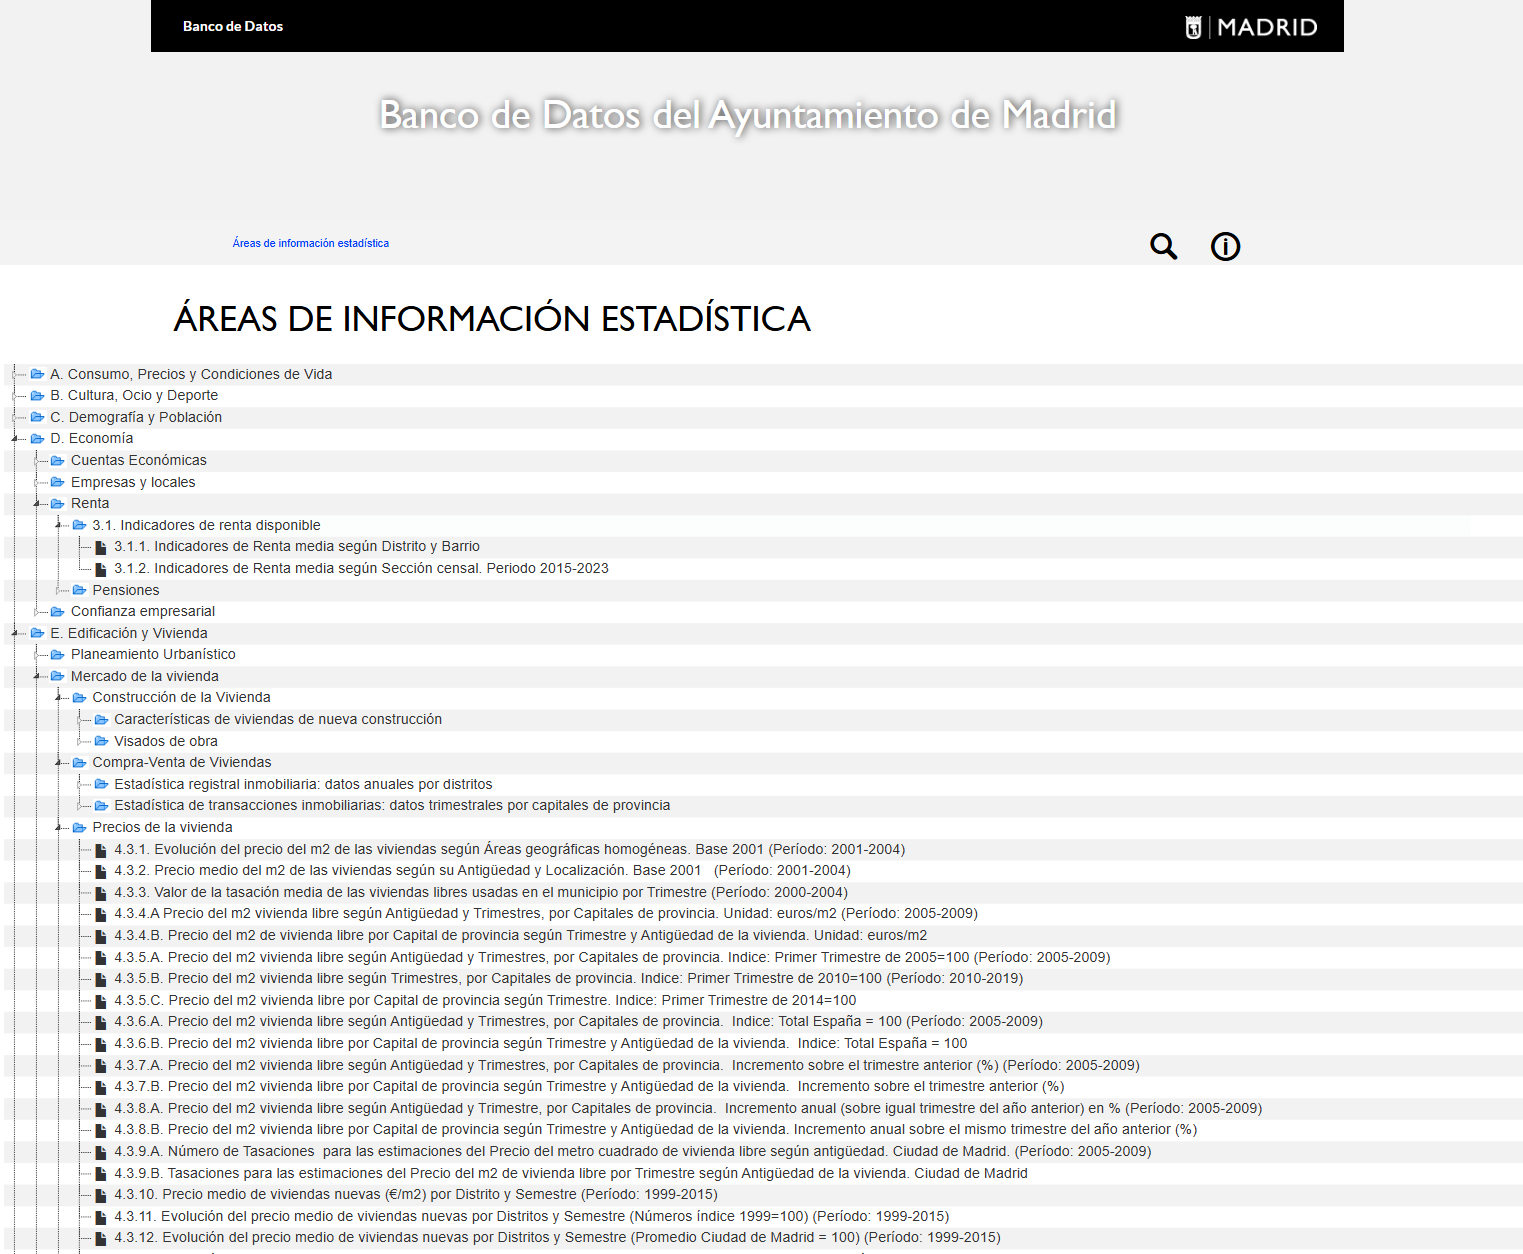
\includegraphics[width=0.90\linewidth]{img/datos_abiertos.png}
\caption{Interfaz del portal estadístico del Banco de Datos del Ayuntamiento de Madrid, utilizado como repositorio oficial para la extracción de indicadores sociodemográficos y económicos.}
\label{fig:portal_datos_abiertos}
\end{figure}

\chapter{Diseño del DataMart}
\label{chap:datamart}
La arquitectura de datos define la organización física y lógica del DataMart, determinando la eficiencia de las consultas analíticas y la capacidad predictiva de la plataforma \textit{Madrid Urban Intelligent}. En este capítulo se detalla la estructura del DataMart, justificando la elección del modelo dimensional y describiendo cada uno de sus componentes, desde las tablas de dimensiones hasta las tablas de hechos de operación y económicos.

\section{Introducción al Modelo Dimensional del DataMart}
La selección de un modelo dimensional para el diseño del DataMart se fundamenta en su eficiencia estructural y su amplia utilización en el desarrollo de almacenes de datos orientados a la analítica (Kimball \& Ross, 2013). Este esquema parte de una configuración en estrella donde una tabla de hechos central se conecta directamente con múltiples tablas de dimensiones laterales, solución que se ha revelado como la más adecuada para el manejo de consultas dinámicas en tiempo real.

La elección de un diseño dimensional en lugar de esquemas más normalizados (como el modelo de copo de nieve) responde a la decisión de simplificar las consultas y maximizar el rendimiento. Al desnormalizar las dimensiones, se reduce considerablemente el número de combinaciones (\textit{joins}) necesarias durante la ejecución de las consultas. Esta mejora en el rendimiento es un factor esencial para una interfaz web interactiva que requiere tiempos de respuesta mínimos para ofrecer una experiencia fluida al usuario.

El propósito central de esta estructura es garantizar la eficiencia de las consultas analíticas y la integridad referencial de los datos, lo que permite que personas con diferentes niveles de conocimiento técnico exploren la información sin enfrentarse a la complejidad de una base de datos relacional tradicional. La estructura bien documentada del modelo garantiza que la comunicación entre la capa de datos y la interfaz de usuario sea directa y eficiente.

No obstante, es importante señalar que este diseño inicial, concebido bajo una topología clásica en estrella, experimentó una evolución posterior durante el proceso de desarrollo. La necesidad de incorporar indicadores macroeconómicos de carácter global, que carecen de granularidad espacial a nivel de distrito o barrio, impulsó la transición del diseño hacia un esquema en constelación con dos tablas de hechos que comparten dimensiones comunes. Esta evolución arquitectónica hace posible integrar variables financieras regionales sin generar redundancia en el almacenamiento; esto anticipa la estructura que se detalla en profundidad en la sección 4.4.

\section{Descripción de las Dimensiones}
Las dimensiones proporcionan el contexto necesario para interpretar las métricas almacenadas en las tablas de hechos. Facilitan segmentar y filtrar la información según criterios temporales y geográficos.

\subsection{Dimensión Tiempo}
La tabla de dimensión \textit{Dim\_Tiempo} se estructura mediante una clave primaria denominada \textit{id\_tiempo} (un entero secuencial que asegura la identificación única de cada período). Esta práctica es el estándar en el modelado dimensional para facilitar uniones rápidas y seguras. La tabla incluye atributos detallados para el año, el mes y el trimestre.

La inclusión del trimestre junto con el año y el mes responde a un requisito analítico específico: la necesidad de identificar ciclos de mercado y variaciones estacionales que no siempre son evidentes en una escala mensual. Mientras que el análisis anual ofrece una perspectiva de largo plazo, el nivel trimestral aporta una visión intermedia fundamental para los informes de coyuntura inmobiliaria. La estructura de esta dimensión es flexible, lo que admite futuras ampliaciones para incluir atributos como el día de la semana o el semestre si las necesidades del proyecto evolucionan.

\begin{figure}[H]
\centering
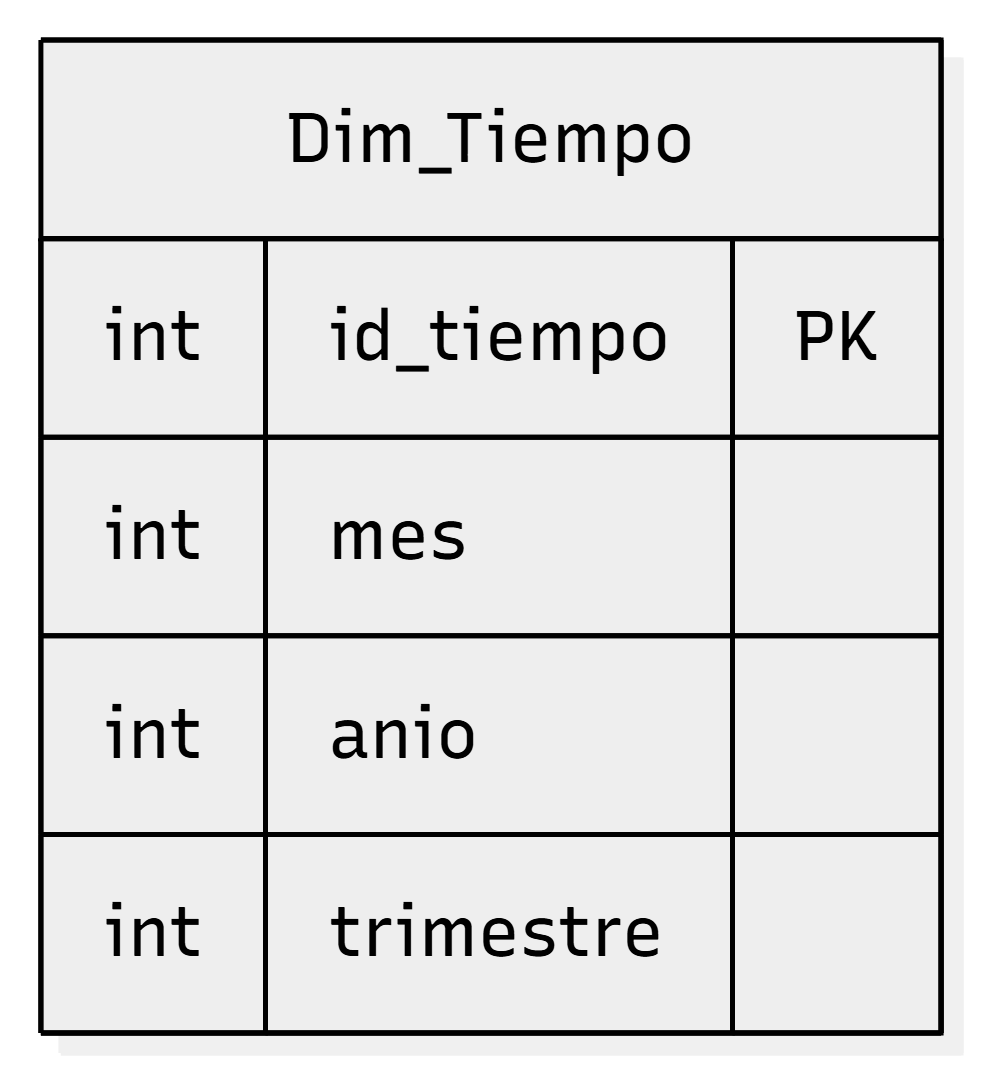
\includegraphics[width=0.29\linewidth]{img/tiempo.png}
\caption{Estructura detallada y atributos de la dimensión Tiempo.}
\label{fig:dim_tiempo}
\end{figure}

\subsection{Dimensión Distrito}
La tabla \textit{Dim\_Distrito} cuenta con el identificador \textit{id\_distrito} como clave primaria. Los campos \textit{codigo} y \textit{nombre} almacenan los datos administrativos oficiales de Madrid, lo que proporciona los atributos esenciales para el filtrado en la interfaz.

Un aspecto diferencial de esta dimensión es la inclusión del atributo \textit{superficie\_media}, que refleja el tamaño promedio de las viviendas en cada distrito. Este dato funciona como un factor contextual crítico, ya que el precio por metro cuadrado de oferta o cierre suele estar influenciado por la tipología predominante y dimensiones promedio en el distrito.

\begin{figure}[H]
\centering
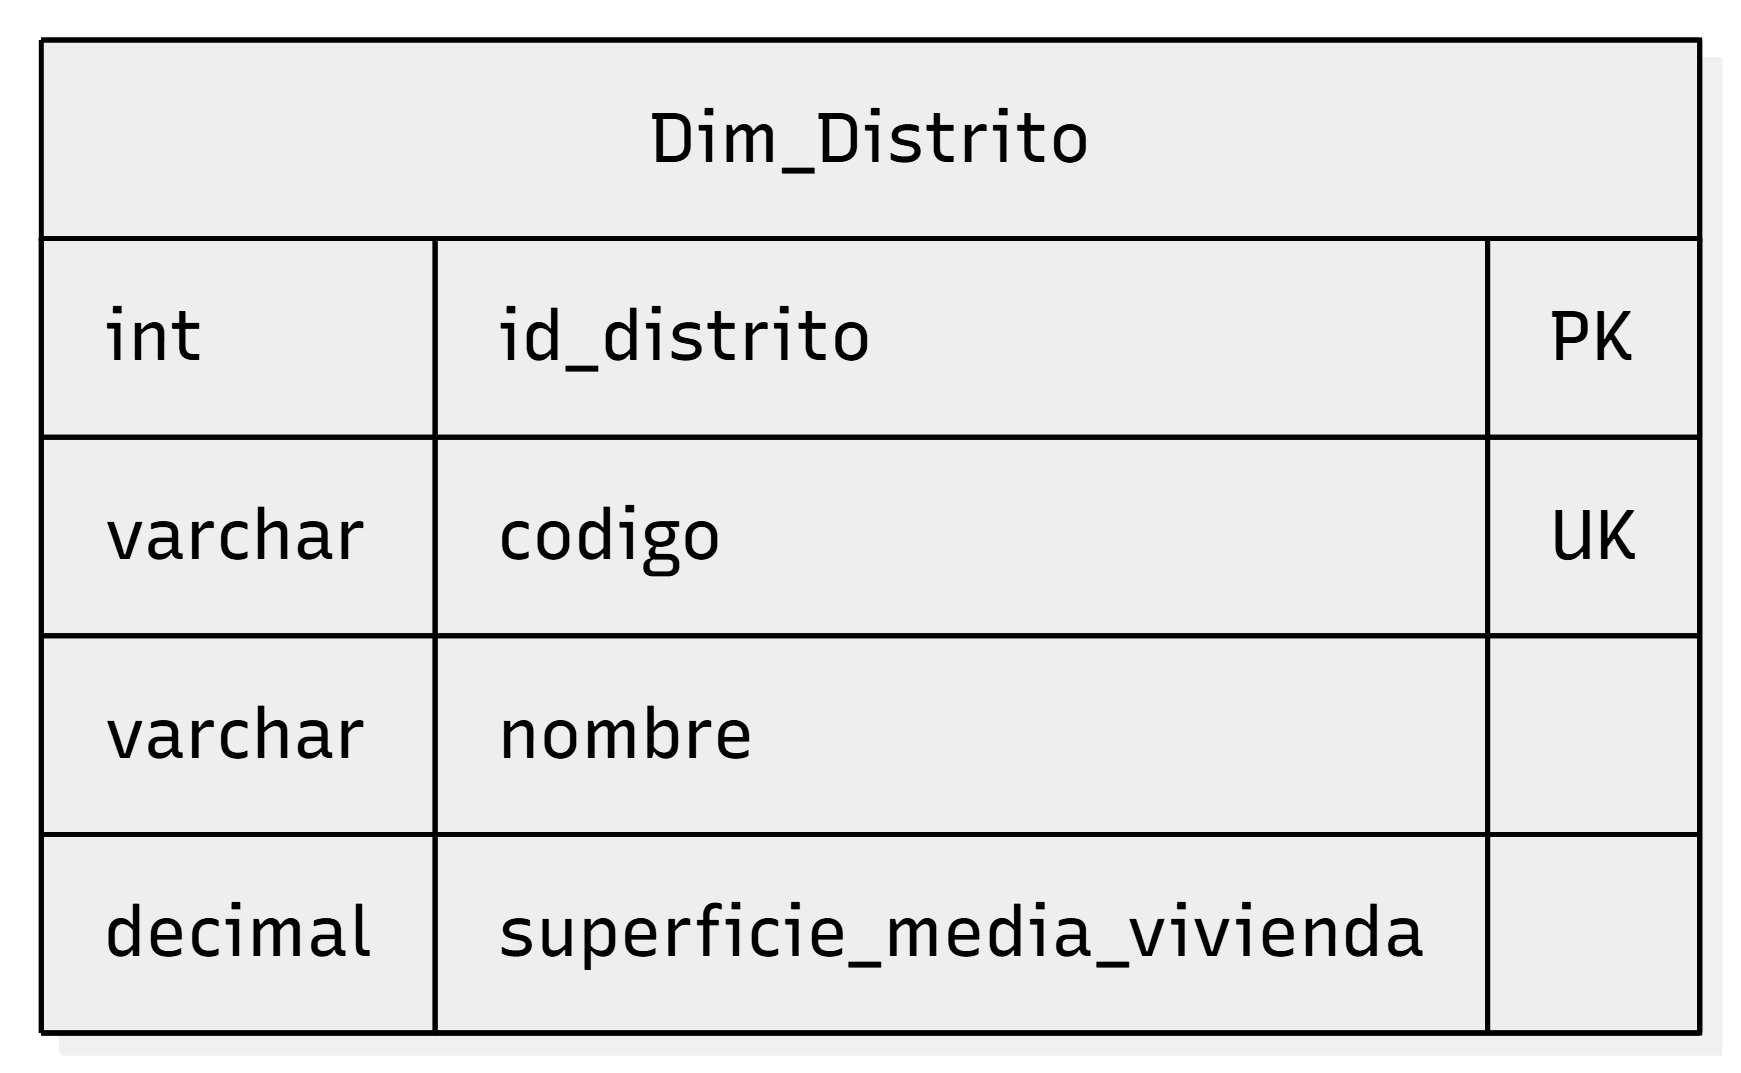
\includegraphics[width=0.40\linewidth]{img/distrito.png}
\caption{Estructura detallada y atributos de la dimensión Distrito.}
\label{fig:dim_distrito}
\end{figure}

\subsection{Dimensión Barrio}
La dimensión \textit{Dim\_Barrio} representa el nivel de granularidad más fino del sistema. Se define mediante la clave \textit{id\_barrio} y almacena los códigos y nombres de los 131 barrios de la capital. La tabla incorpora la clave foránea \textit{id\_distrito} para establecer la jerarquía administrativa; esto da la opción al usuario de navegar (realizar un \textit{drill-down}) desde la visión general del distrito hasta los detalles específicos del barrio.

Al igual que en la dimensión superior, se incluye la superficie media a nivel de barrio. Esta decisión de diseño reconoce que, incluso dentro de un mismo distrito, existen micro-mercados residenciales con características muy distintas. Al proporcionar esta granularidad, la plataforma facilita la detección de oportunidades o riesgos que podrían quedar enmascarados si solo se observaran los promedios distritales.

\begin{figure}[H]
\centering
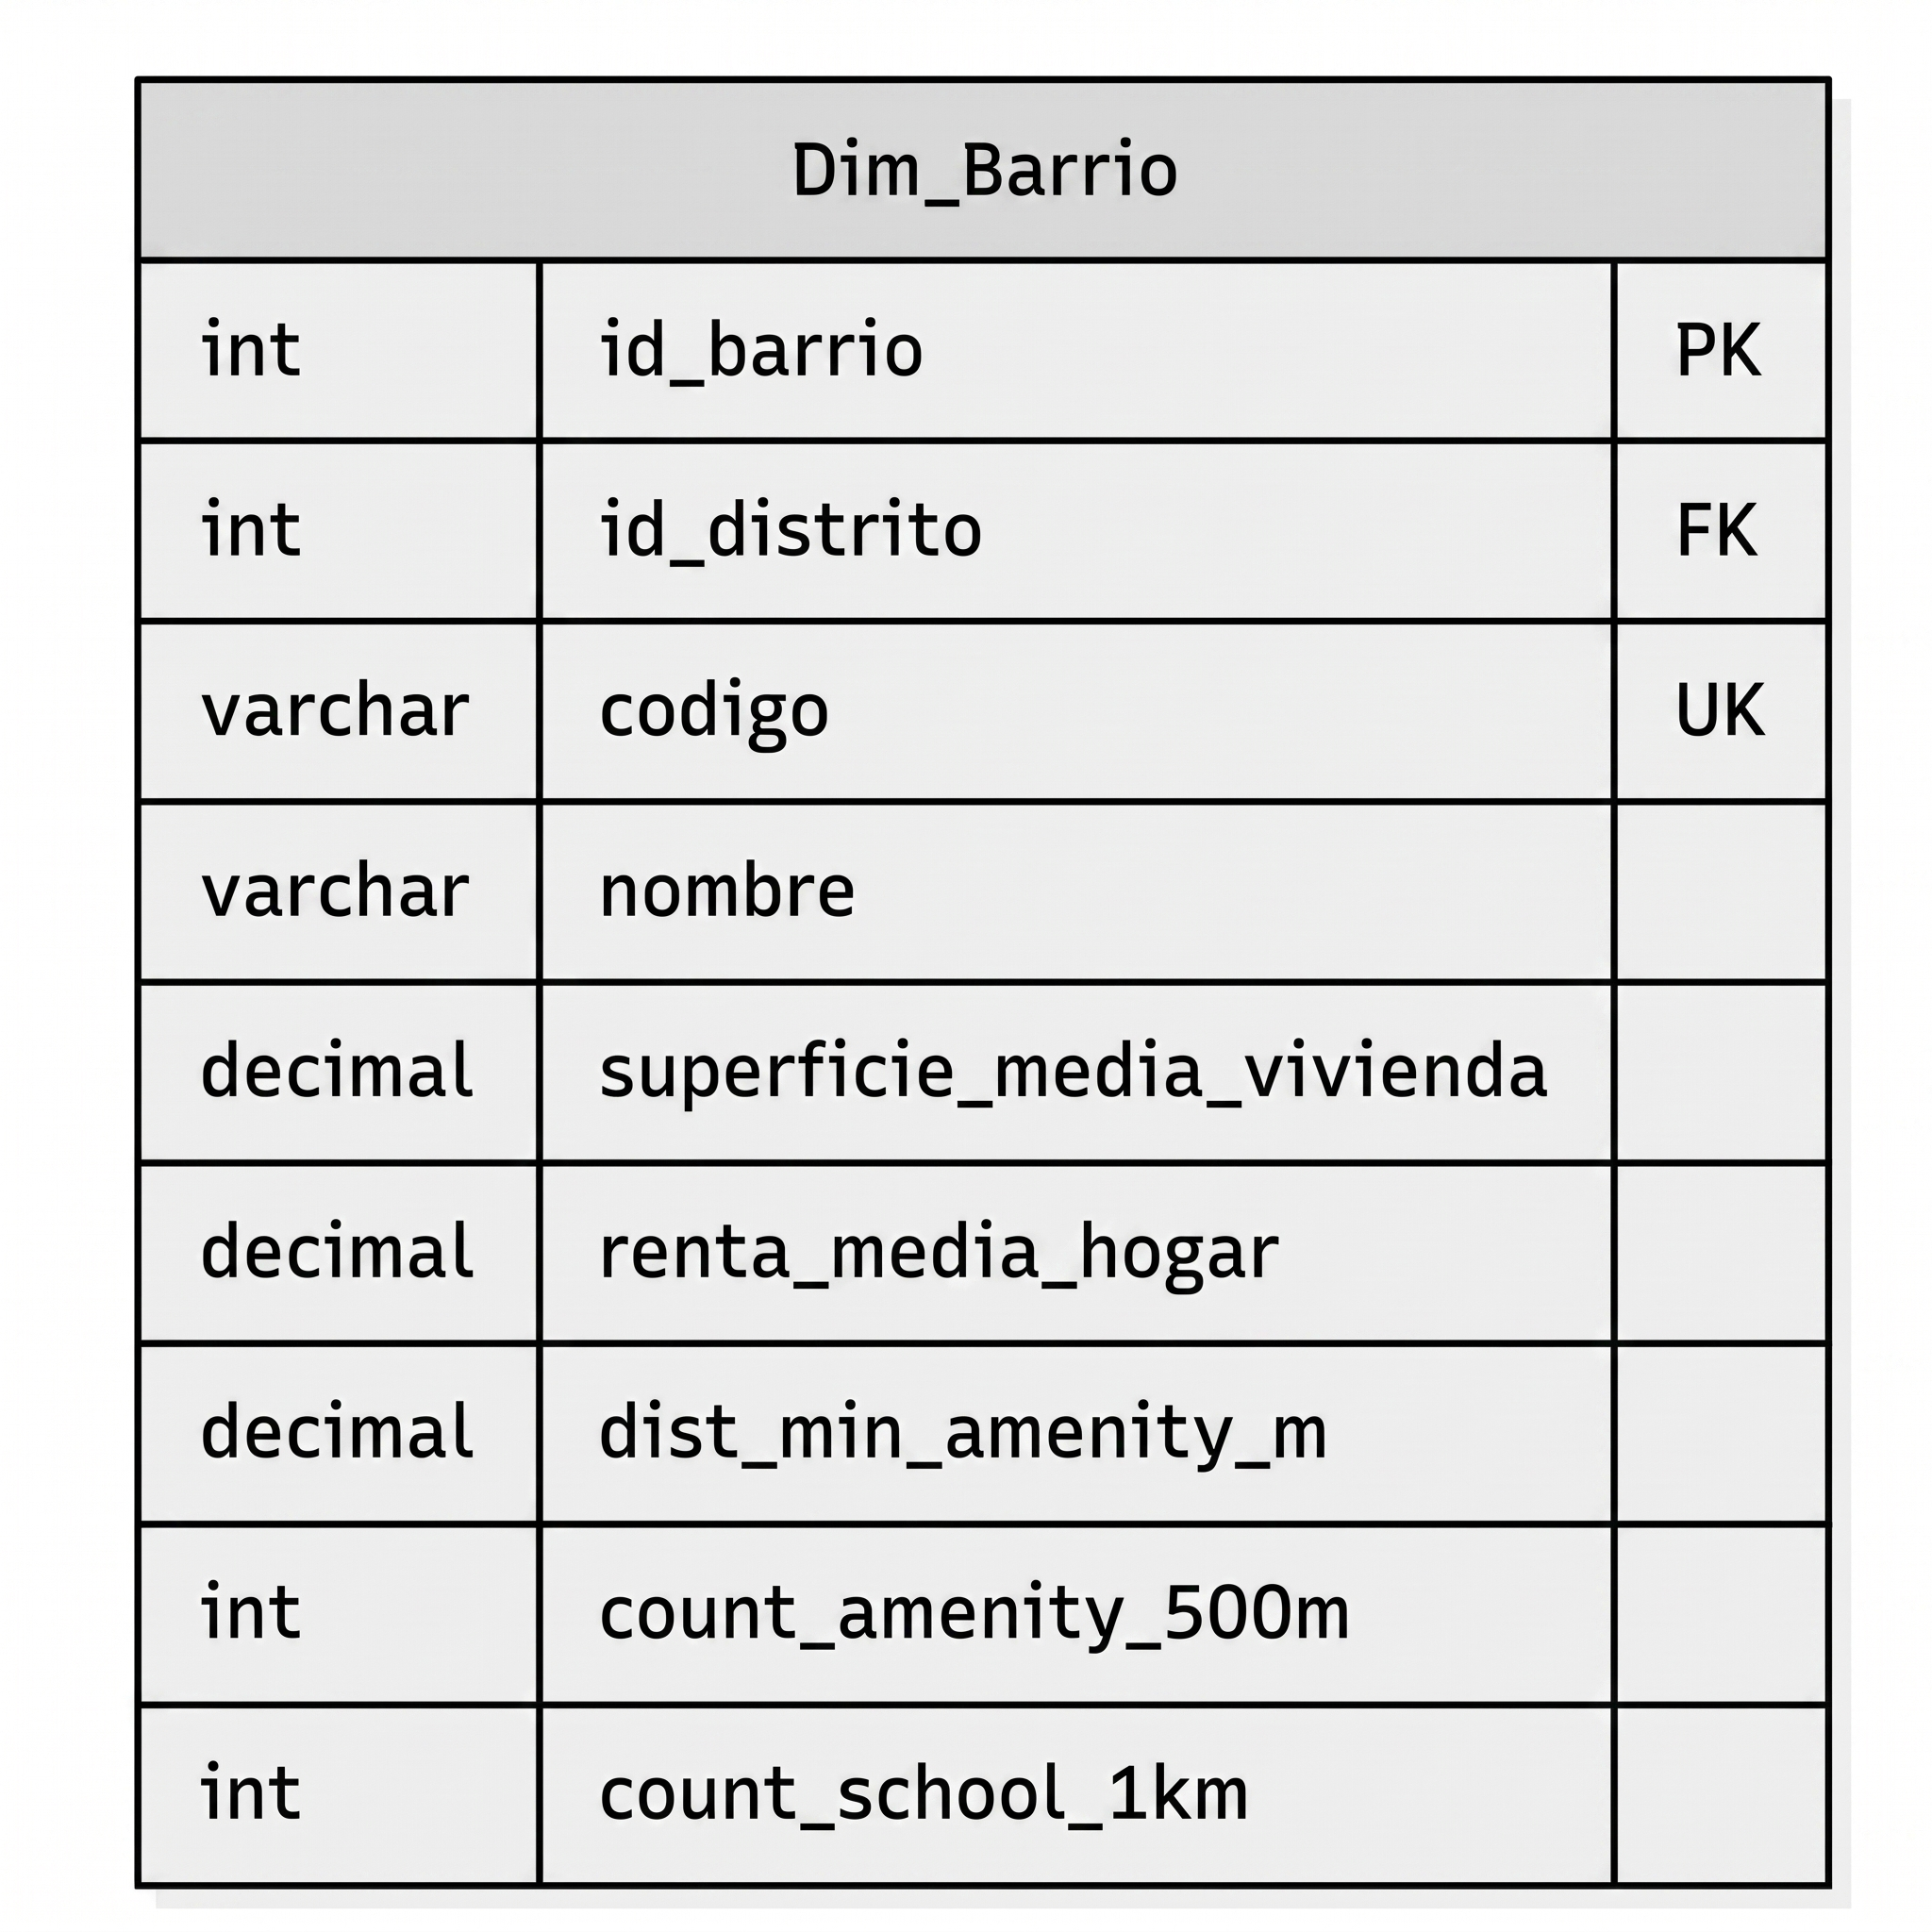
\includegraphics[width=0.37\linewidth]{img/barrio.png}
\caption{Estructura detallada y atributos de la dimensión Barrio, incluyendo variables socioeconómicas y geoespaciales.}
\label{fig:dim_barrio}
\end{figure}

\section{Descripción de las Tablas de Hechos}
Las tablas de hechos son el núcleo del DataMart, donde se almacenan las métricas cuantitativas que reflejan la realidad del sector.

\subsection{Hechos de Operación}
La tabla \textit{Fact\_Operacion} constituye el eje central del modelo. Su objetivo es capturar y evaluar las principales métricas vinculadas a las transacciones inmobiliarias. En ella se almacenan indicadores clave como el \textit{precio\_m2}, las variaciones porcentuales mensuales, trimestrales y anuales, la métrica de volumen \textit{num\_transacciones} (que registra el total de compraventas mensuales reales consolidadas a nivel de distrito para reflejar la liquidez y dinamismo de cada mercado) y el campo calculado \textit{rentabilidad\_bruta}, que registra la rentabilidad bruta anual del arrendamiento respecto al precio de venta y es actualizado por el script \textit{calc\_yield.py}.

La inclusión directa de estas métricas de variación y volumen en la tabla de hechos es una decisión estratégica para acelerar el análisis de tendencias. En un entorno predictivo, estas variaciones y volúmenes funcionan como señales tempranas del comportamiento de la oferta y la demanda. Además, la tabla incorpora métricas calculadas como el \textit{precio\_promedio\_vivienda} (basado en la superficie media) y el \textit{total\_anual}, lo que proporciona una base robusta para el estudio cuantitativo y la generación de informes dinámicos. La tabla se enlaza mediante claves foráneas con las dimensiones de tiempo, distrito y barrio, lo que habilita una exploración multidimensional completa.

\begin{figure}[H]
\centering
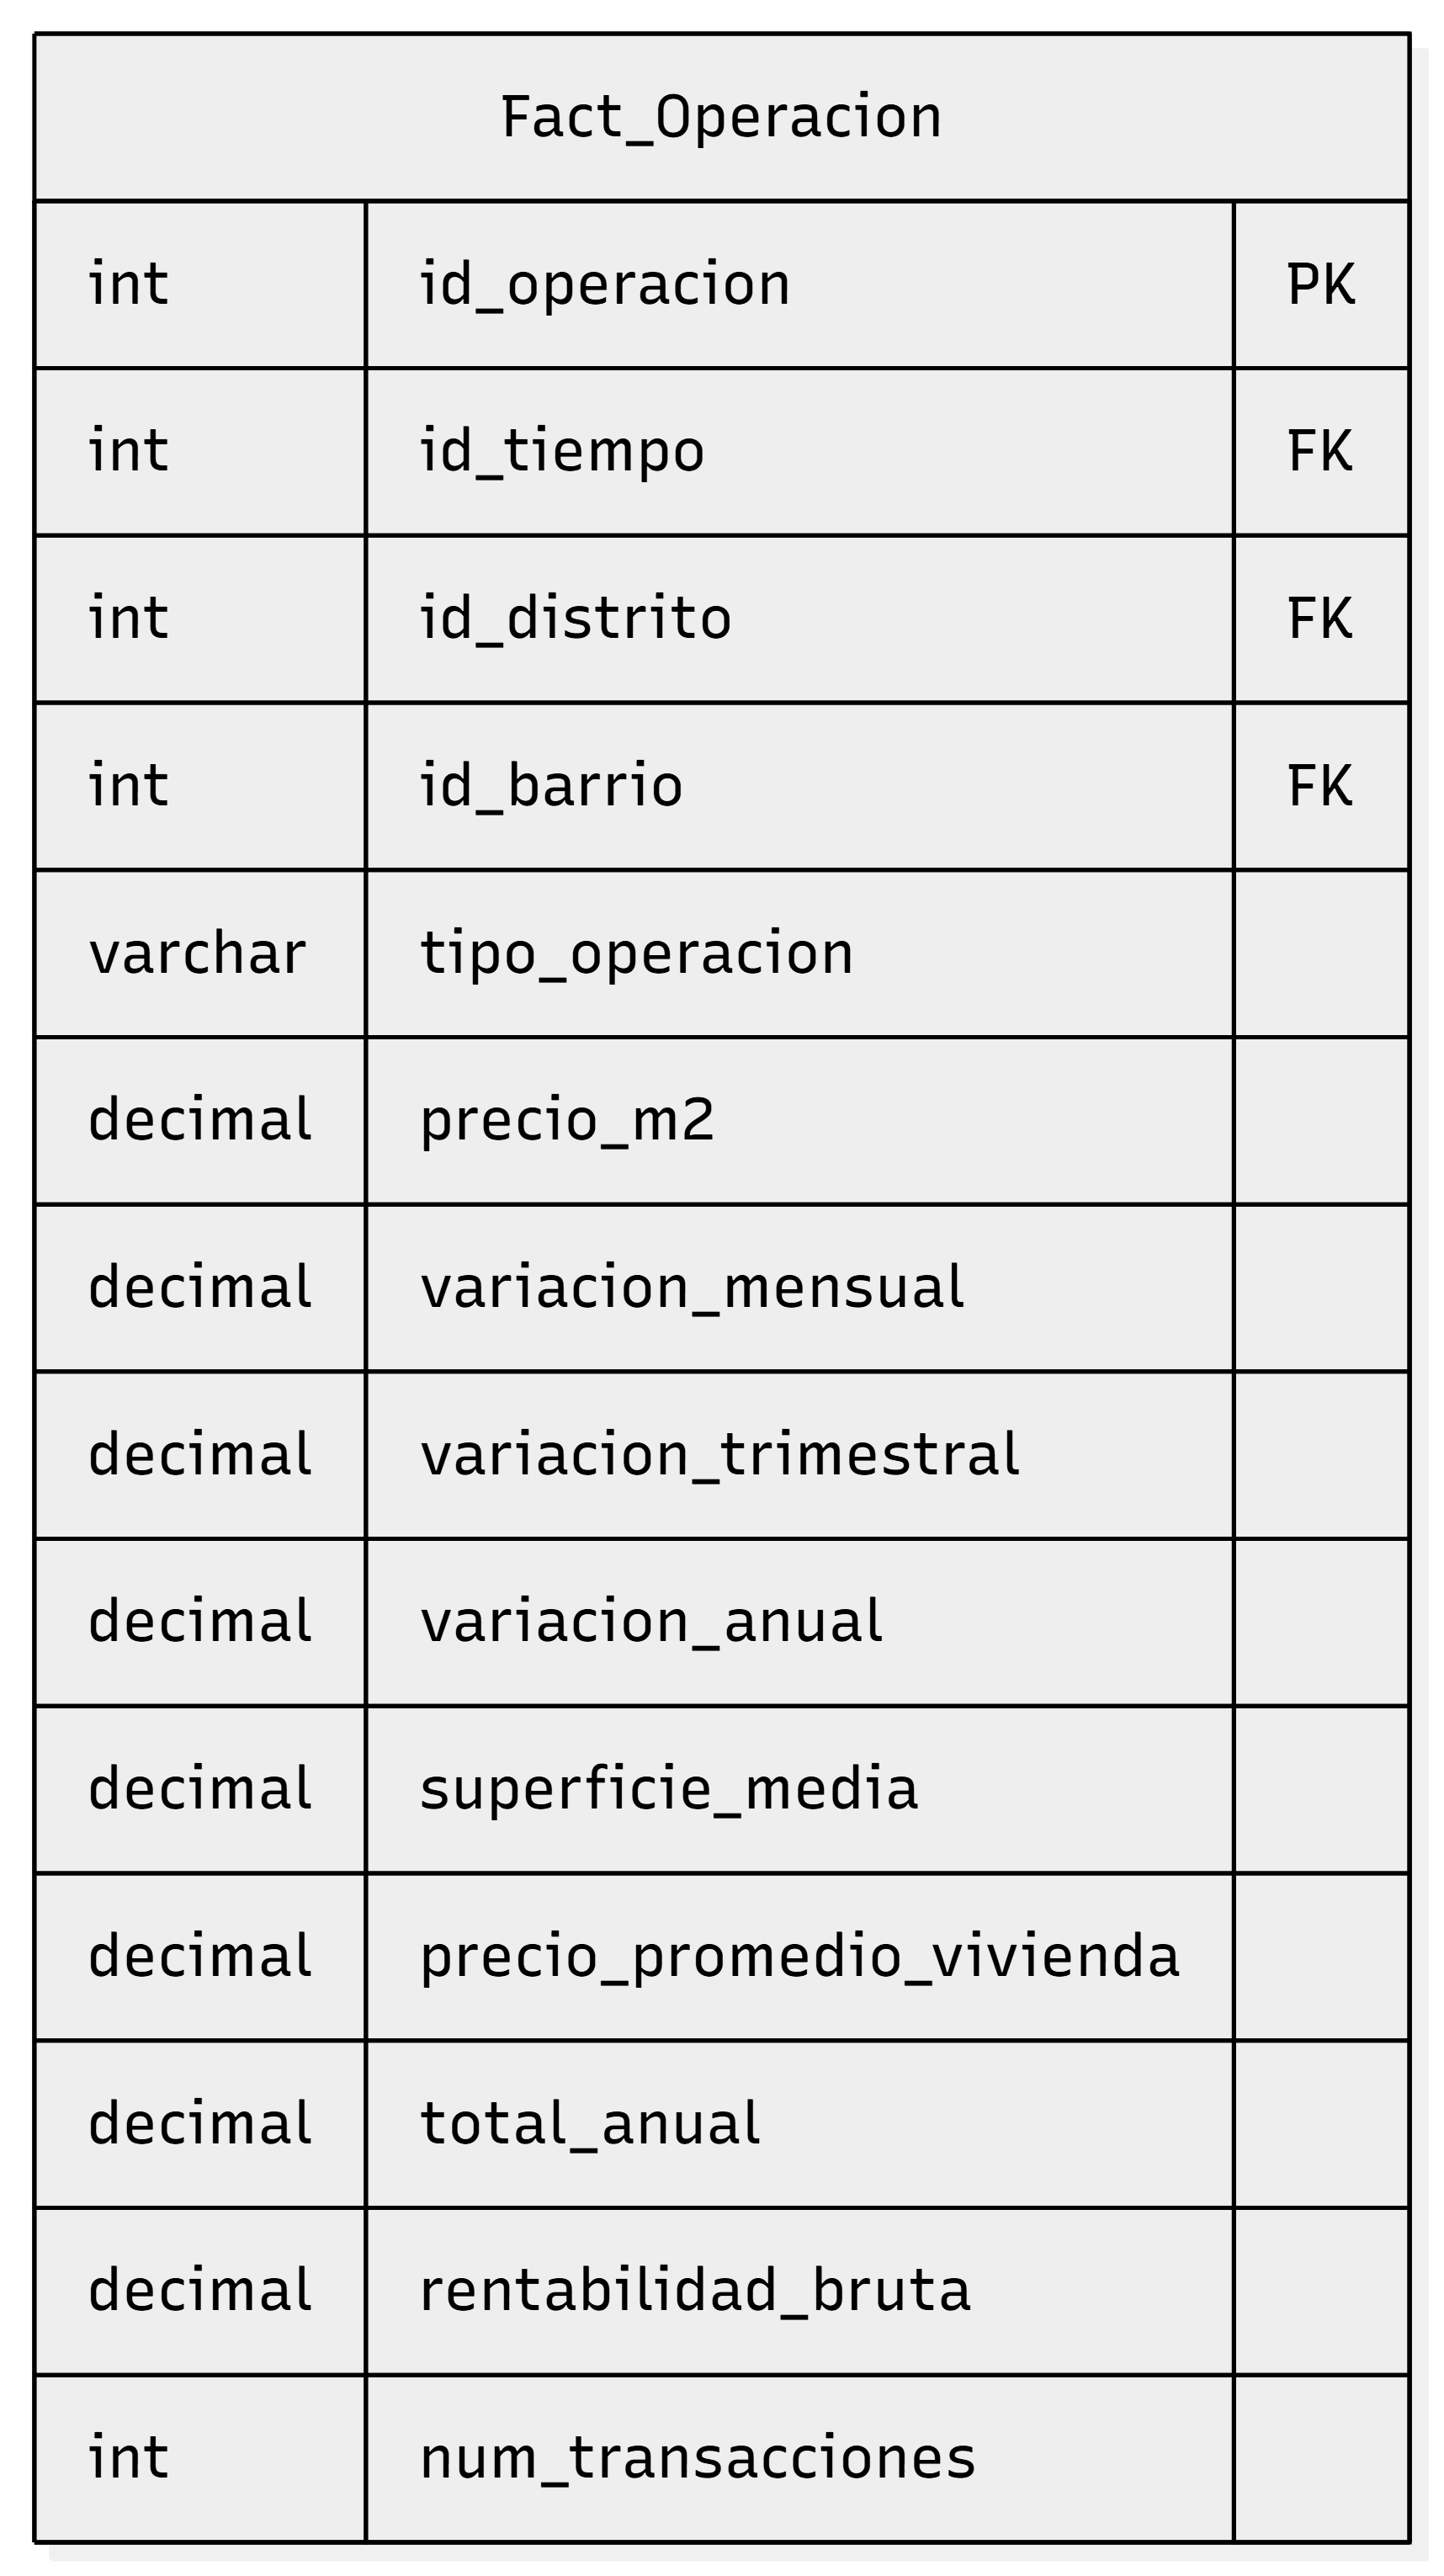
\includegraphics[width=0.32\linewidth]{img/operacion.png}
\caption{Estructura de la tabla de hechos de Operaciones con claves de dimensiones y métricas de mercado.}
\label{fig:Fact_Operacion}
\end{figure}

\subsection{Hechos Económicos}
La tabla \textit{Fact\_Economica} se ha diseñado para integrar indicadores macroeconómicos que impactan directamente en el sector inmobiliario. Incluye métricas como el Euríbor a un año, el tipo de interés de referencia del Banco de España y la cuota hipotecaria media mensual, tal como se detalla en la tabla de fuentes del Capítulo~\ref{chap:datos}. Estos factores externos son determinantes para contextualizar los movimientos de precios y mejorar la precisión de los pronósticos.

En comparación con los hechos de operación, esta tabla solo se enlaza con la dimensión temporal (\textit{id\_tiempo}), bajo la premisa de que los indicadores macroeconómicos se consideran a nivel agregado para toda la región de Madrid. Esta separación resalta el impacto de las condiciones externas globales sobre la dinámica interna del mercado local.

\begin{figure}[H]
\centering
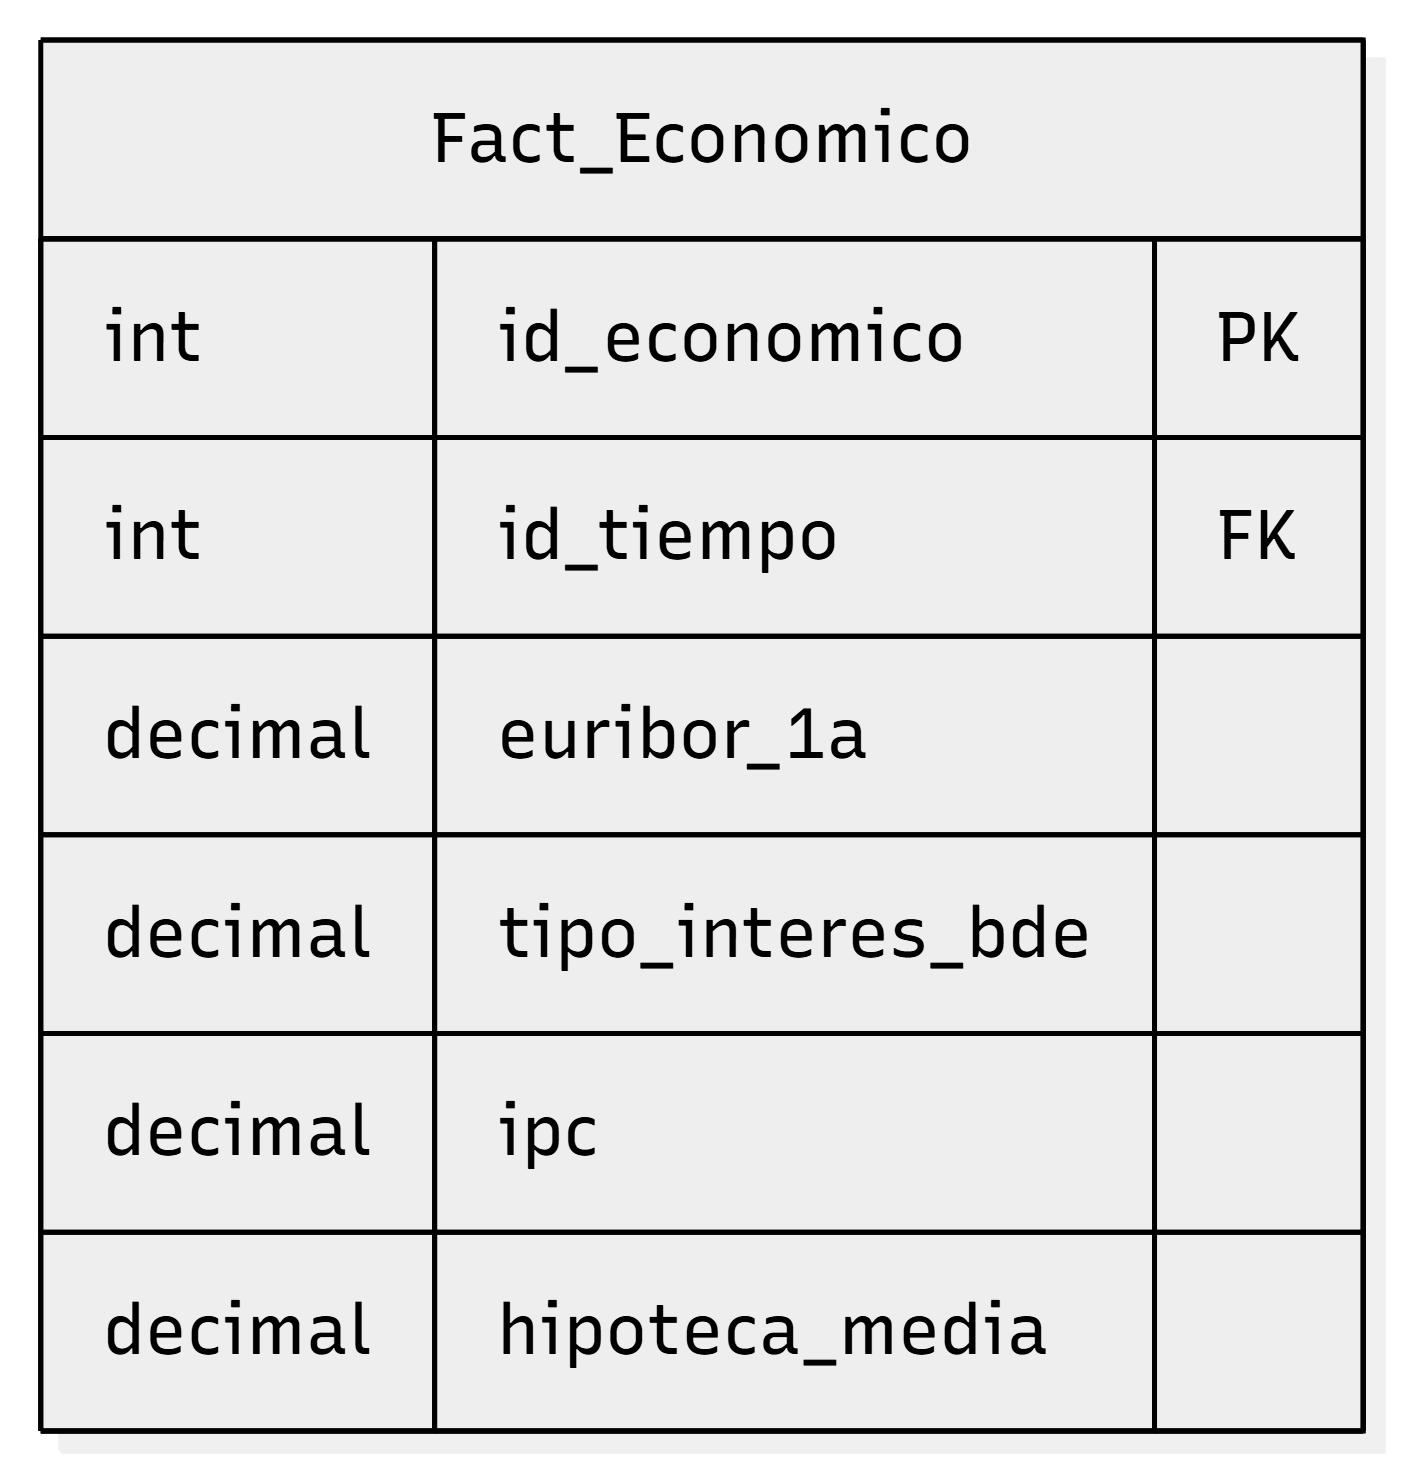
\includegraphics[width=0.30\linewidth]{img/economico.png}
\caption{Estructura de la tabla de hechos Económicos con enlace único a la dimensión temporal.}
\label{fig:fact_economico}
\end{figure}

\section{Integridad Referencial y Evolución a Esquema en Constelación}
Para garantizar la coherencia absoluta de los datos, el diseño original del DataMart ha evolucionado hacia un modelo avanzado de esquema en constelación (Fact Constellation o Galaxy Schema). Frente a una topología en estrella tradicional, este diseño contempla la coexistencia e interconexión de múltiples tablas de hechos (en este caso, \textit{Fact\_Operacion} y \textit{Fact\_Economica}) que comparten de forma eficiente las dimensiones comunes del sistema.

La integridad referencial se mantiene estrictamente en toda la constelación mediante el uso de claves primarias autogeneradas y restricciones de claves foráneas. Específicamente, este enfoque arquitectónico se justifica a través de los siguientes pilares de diseño físico y analítico:

\begin{itemize}
    \item \textbf{Capa Temática y Espacial Compartida:} Las tablas de dimensiones principales (\textit{Dim\_Tiempo}, \textit{Dim\_Distrito} y \textit{Dim\_Barrio}) actúan como los ejes unificadores sobre los cuales se estructuran los hechos, lo que evita duplicidades de catálogos y facilita uniones relacionales de alto rendimiento para el posterior entrenamiento de los modelos predictivos.
    \item \textbf{Hechos de Operación Enriquecidos:} La tabla \textit{Fact\_Operacion} se enriquece con la variable \textit{num\_transacciones}. Esta registra el volumen mensual de compraventas reales del Colegio de Registradores a nivel de distrito, integrando una métrica de liquidez en las transacciones hiperlocales.
    \item \textbf{Constelación de Hechos Económicos:} La tabla de hechos macroeconómicos y financieros (\textit{Fact\_Economica}) centraliza indicadores de escala regional y mensual (como Euríbor, tipos de interés del Banco de España, IPC e hipoteca media) enlazándose con la dimensión temporal (\textit{Dim\_Tiempo}). Esto elimina la redundancia masiva que se produciría al duplicar métricas globales en cada uno de los 131 barrios.
    \item \textbf{Dimensión de Barrio Socioeconómica:} La dimensión espacial de nivel granular (\textit{Dim\_Barrio}) incorpora la variable \textit{renta\_media\_hogar} (Renta Neta Media por Hogar). Esto dota al datamart de la profundidad socioeconómica indispensable para el modelado algorítmico y la exploración de gradientes de riqueza urbana.
\end{itemize}

Esta arquitectura en constelación elimina dependencias redundantes y optimiza el rendimiento de las consultas transversales entre las dos tablas de hechos, reduciendo la latencia de respuesta tanto en los cuadros de mando como en el motor conversacional de la plataforma.

\begin{figure}[H]
\centering
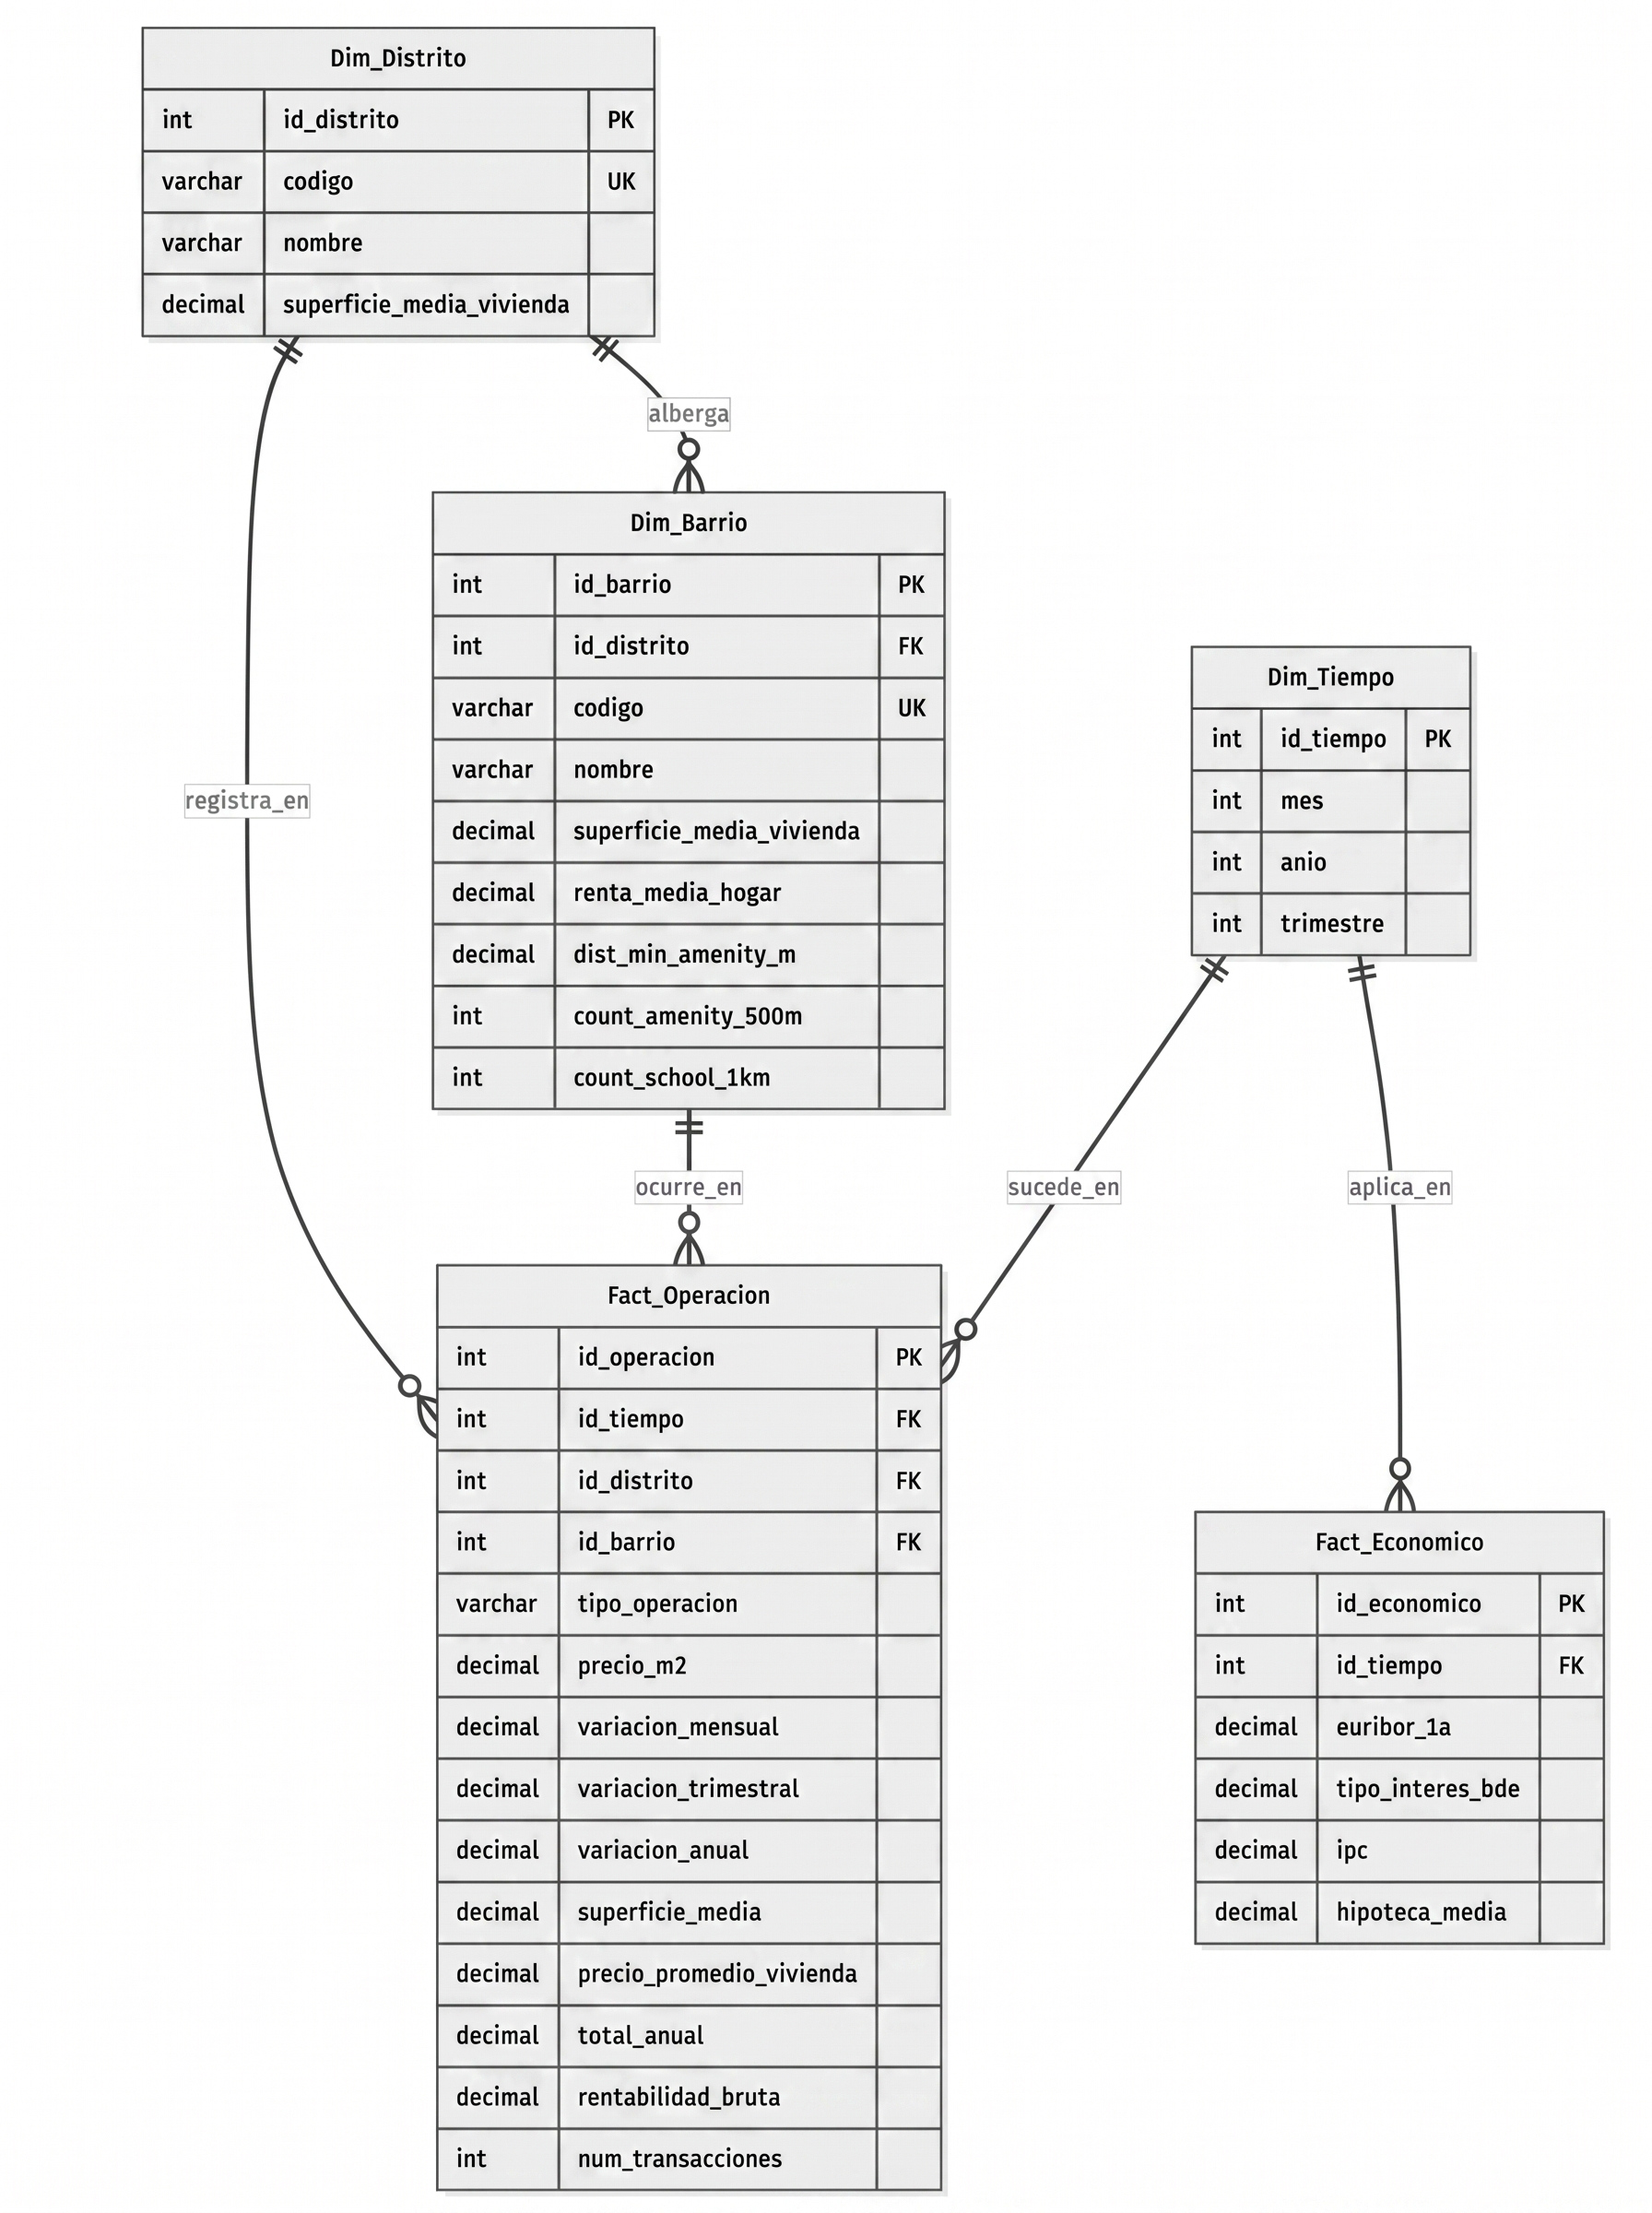
\includegraphics[width=0.60\linewidth]{img/diagrama_datamart.png}
\caption{Diagrama lógico-dimensional del DataMart en esquema de constelación (Kimball \& Ross, 2013). Se muestran los atributos principales por claridad visual; el esquema completo, incluyendo variables de proximidad y densidad de equipamientos urbanos, se describe en el Capítulo~\ref{chap:etl}.}
\label{fig:diagrama_datamart}
\end{figure}

\chapter{Diseño e Implementación del Proceso ETL}
\label{chap:etl}
El proceso de Extracción, Transformación y Carga (ETL) constituye la infraestructura técnica central de la plataforma \textit{Madrid Urban Intelligent}. En el ámbito de la ciencia de datos urbana, el desarrollo de capacidades analíticas avanzadas, el modelado predictivo de aprendizaje automático y la interacción conversacional basada en lenguaje natural exigen un flujo de datos continuo, auditable y de alta integridad. Frente a las aproximaciones tradicionales basadas en procesos manuales o herramientas de software propietario, este proyecto implementa un conjunto integrado de scripts en Python que automatiza desde la adquisición primaria de la información en repositorios administrativos y portales comerciales hasta su enriquecimiento geoespacial multiescalar y su consolidación final en el DataMart físico relacional. Este capítulo describe minuciosamente el diseño, la formulación matemática de los indicadores calculados, las reglas lógicas de depuración e imputación espacial, y la orquestación del pipeline que garantiza la robustez y reproducibilidad científica de la base de datos analítica del sistema.

\section{Introducción al Pipeline ETL}
El pipeline ETL de este proyecto ha sido concebido como un motor de ingeniería de datos unificado que automatiza la ingesta de fuentes de datos heterogéneas (formatos CSV, XLS, APIs y cartografía vectorial) para poblar y sincronizar de forma coherente las cinco tablas que componen la topología analítica en constelación del DataMart analítico: las dimensiones estructuradas \textit{Dim\_Tiempo}, \textit{Dim\_Distrito} y \textit{Dim\_Barrio}, y las tablas de hechos compartidas \textit{Fact\_Operacion} y \textit{Fact\_Economica}. 

La dimensión temporal (\textit{Dim\_Tiempo}) se inicializa mediante un procedimiento programático interno en SQLite que asegura una serie cronológica perfecta libre de discontinuidades. Por su parte, el resto de las entidades del sistema dependen directamente de la ejecución secuencial y la orquestación de un conjunto de scripts en Python que resuelven de forma transparente la normalización semántica, la limpieza de inconsistencias tipográficas, la resolución de la integridad referencial espacial y el cálculo dinámico de variables externas. Este flujo integrado se expone de manera detallada a través de las fases de extracción, transformación, carga y enriquecimiento descritas a continuación.

\section{Fase de Extracción Automatizada (Extract)}
La fase de extracción representa el primer eslabón del pipeline y determina la fiabilidad de los datos de entrada. En el entorno de la administración pública española, los portales oficiales de datos abiertos, si bien ofrecen información de gran valor, carecen con frecuencia de interfaces de programación públicas y gratuitas (\textit{APIs REST}) dinámicas, y publican sus series históricas mediante interfaces web interactivas propensas a cambios de diseño, redirecciones de enlace y caducidad de tokens de sesión, lo cual impide el uso de librerías de petición HTTP estándar como \textit{requests} o \textit{urllib}.

\begin{figure}[H]
\centering
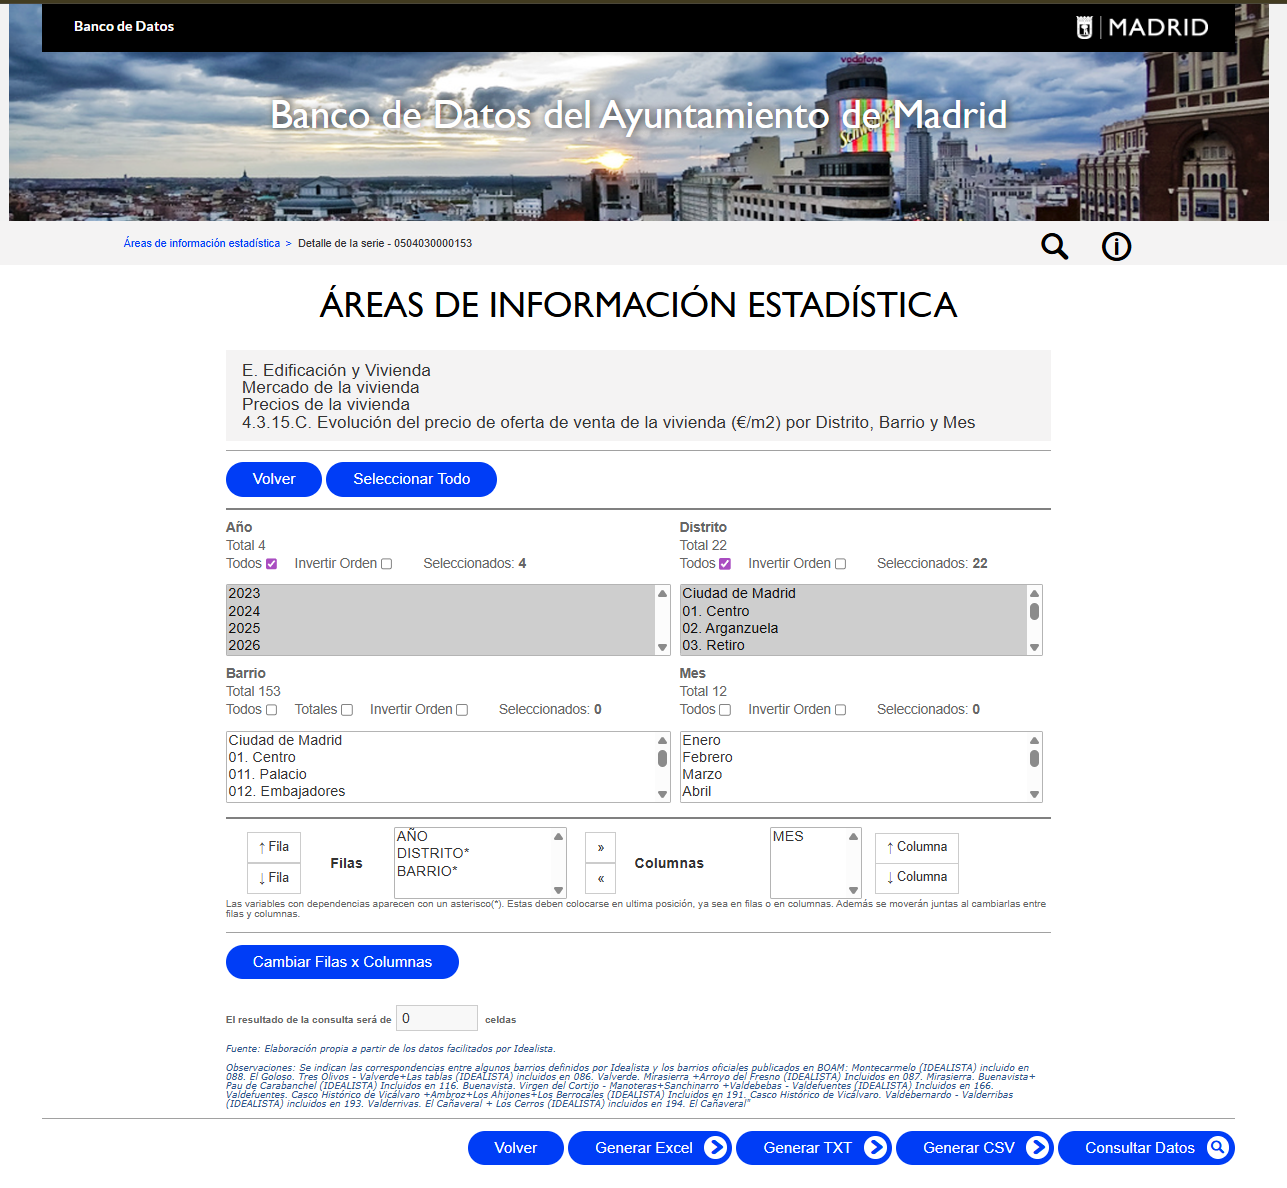
\includegraphics[width=0.70\linewidth]{img/formulario_datos.png}
\caption{Interfaz del formulario de datos en el portal municipal para la selección y descarga de series históricas de precios.}
\label{fig:formulario_datos}
\end{figure}

\subsection{Automatización de Captura mediante Playwright}
Para superar estas barreras técnicas y garantizar una captura de datos robusta y dinámica, se ha desarrollado el script de extracción automatizada \textit{download\_ayto.py}, que emplea la biblioteca de automatización web \textit{Playwright} (Microsoft, 2020) para superar las restricciones de las interfaces web municipales. Playwright se conecta directamente al motor de renderizado del navegador a través del protocolo nativo \textit{Chrome DevTools Protocol} (CDP), lo que evita depender de la arquitectura cliente-servidor de Selenium basada en peticiones HTTP sucesivas. 

Esta conexión directa hace posible una comunicación bidireccional y asíncrona de baja latencia que facilita al script el control de eventos complejos en la página web. El script implementa un navegador sin cabeza (\textit{headless browser}) que emula el comportamiento de un usuario humano: accede al portal municipal, interactúa con los menús desplegables del Banco de Datos, gestiona de forma nativa las esperas de renderizado de elementos asíncronos en JavaScript mediante mecanismos de espera automática (\textit{auto-waiting}), elude bloqueos por políticas de seguridad e inicia la descarga directa de los archivos fuente tabulares en formato CSV y Excel, guardándolos en la carpeta temporal de datos brutos del proyecto (\textit{data/raw/}).

\begin{figure}[H]
\centering
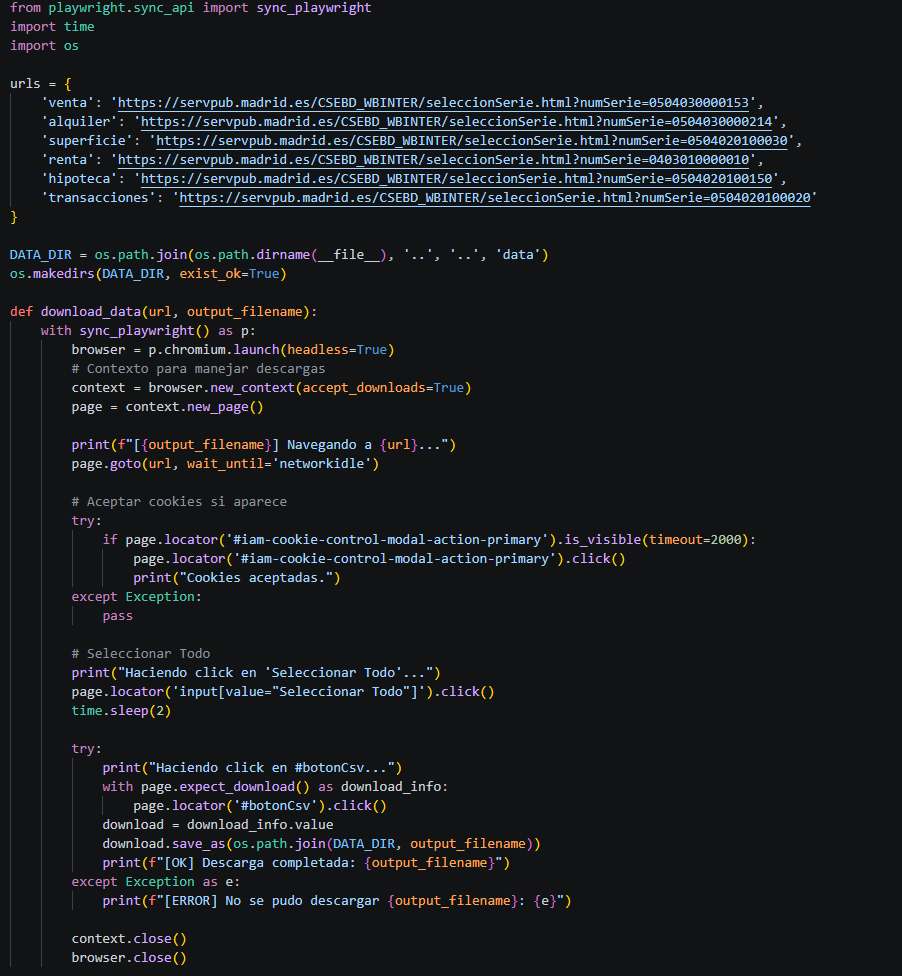
\includegraphics[width=0.63\linewidth]{img/5.2.1.download_ayto.png}
\caption{Código fuente del script download\_ayto\_2.py implementado con Playwright para descargas asíncronas del portal municipal.}
\label{fig:playwright_code}
\end{figure}

\subsection{Orígenes y Gestión de las Series de Datos Reales}
El pipeline de extracción se ha configurado para descargar de forma sistemática seis conjuntos de datos reales y oficiales indispensables para conformar la base física, socioeconómica y macroeconómica de la constelación. Cada una de estas series se extrae mediante identificadores de serie e índices registrales oficiales del Ayuntamiento de Madrid y del Banco de España:
\begin{enumerate}
    \item \textbf{Evolución del precio de venta de vivienda (Código 0504030000153):} Serie mensual en euros por metro cuadrado, desglosada con la máxima granularidad a nivel de distrito y barrio desde enero de 2023. Aporta el histórico dinámico de compraventa oficial de la capital.
    \item \textbf{Evolución del precio de alquiler de vivienda (Código 0504030000214):} Serie mensual en euros por metro cuadrado por distrito y barrio, lo que proporciona la contraparte transaccional para el estudio del arrendamiento y la rentabilidad del suelo.
    \item \textbf{Superficie media de las viviendas (Código 0504020100030):} Fichero anual con desglose por distritos y barrios que registra la dimensión física promedio en metros cuadrados construidos de las viviendas madrileñas, un factor clave para estimar los precios totales de adquisición.
    \item \textbf{Renta neta media por hogar (Código 0403010000010):} Indicador socioeconómico del Portal de Datos Abiertos del Ayuntamiento que registra los ingresos anuales promedio familiares a escala hiperlocal de sección censal y barrio, lo que aporta la variable de capacidad de pago.
    \item \textbf{Volumen mensual de transacciones inmobiliarias (Código 0504020100020):} Estadísticas reales agregadas del Colegio de Registradores de España que registran la cifra exacta de compraventas firmadas y formalizadas ante notario a nivel de distrito, lo que aporta un indicador crítico de liquidez.
    \item \textbf{Euríbor, Importe Medio de Hipotecas e Intereses (Código 0504020100150):} Serie macroeconómica del Banco de España que recoge la fluctuación del Euríbor a un año, los tipos de interés de referencia del crédito hipotecario y el importe medio del crédito constituido mensualmente en Madrid.
\end{enumerate}

\section{Fase de Transformación Compleja (Transform)}
La fase de transformación unifica las fuentes brutas heterogéneas bajo reglas estrictas de limpieza, conversión de tipos, integridad referencial y enriquecimiento matemático, lo que asegura que el DataMart contenga exclusivamente registros normalizados listos para su explotación predictiva y conversacional.

\subsection{Pivotado de Formato Ancho a Largo (Wide-to-Long)}
Los archivos de precios y superficies de origen municipal presentan una estructura de diseño orientada a la lectura humana y no al almacenamiento analítico relacional. Específicamente, se estructuran mediante un formato ancho o matricial, donde las filas representan el año y la zona geográfica (distrito/barrio), y cada uno de los doce meses del año constituye una columna independiente con su respectivo valor de precio. 

Para resolver esta anomalía física y normalizar los datos al diseño del modelo dimensional, el script \textit{clean\_ayto.py} implementa una lógica de pivotado basada en la función \texttt{melt} de la biblioteca \textit{pandas} en Python (McKinney, 2010). El proceso desestructura la matriz mensual y la transpone en una estructura de formato largo (\textit{long format}), donde cada registro representa una observación única de corte temporal y espacial definida por las variables \texttt{(id\_tiempo, cod\_distrito, cod\_barrio, Precio\_m2)}, lo que simplifica las consultas de agregación temporal en el DataMart y facilita una modelación temporal ágil para la inteligencia artificial.

\begin{figure}[H]
\centering
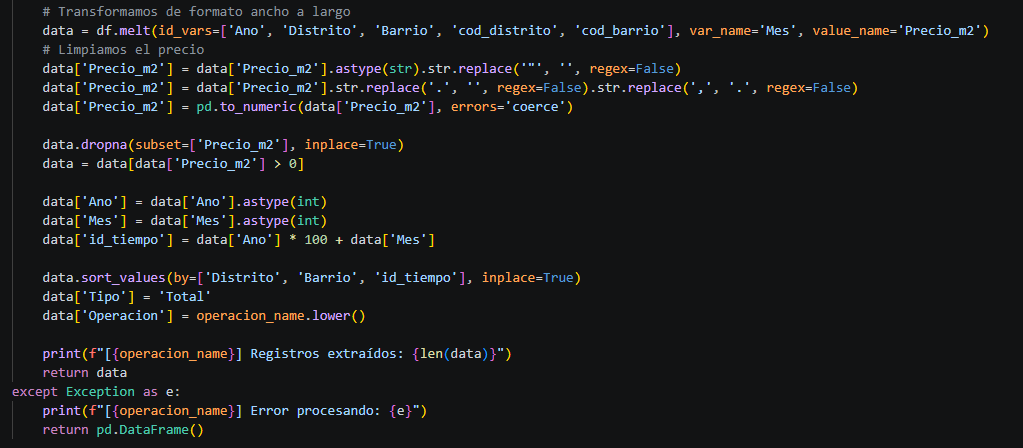
\includegraphics[width=0.85\linewidth]{img/5.3.2.tranformacion_formato_ancho_largo.png}
\caption{Código del script clean\_ayto.py que muestra la transposición de datos mediante el método melt de pandas.}
\label{fig:melt_code}
\end{figure}

\subsection{Depuración de Agregados del Distrito y del Municipio}
Un desafío de calidad identificado durante la fase de análisis fue que las series brutas del Ayuntamiento contienen filas de agregación espacial acumulativa. Por un lado, incluyen la categoría global \textit{``Ciudad de Madrid''} para reflejar la media general de todo el término municipal. Por otro lado, en los archivos desglosados por barrios, se inserta una fila resumen del distrito donde el nombre del barrio coincide exactamente con el del distrito, y comparten el mismo código de zona. 

Para prevenir una duplicidad masiva de registros (que sesgaría cualquier cálculo promedio del mercado inmobiliario), el script de transformación aplica dos filtros de exclusión estrictos:
\begin{itemize}
    \item \textbf{Exclusión municipal global:} Se eliminan mediante expresiones regulares insensibles a mayúsculas todas las filas donde las variables de distrito o barrio contengan la cadena \textit{``ciudad de madrid''}.
    \item \textbf{Resolución de jerarquía y descarte de duplicados de distrito:} Para los registros correspondientes al resumen general del distrito (donde \texttt{cod\_barrio == cod\_distrito}), se aplica un descarte sistemático en la dimensión espacial de barrios de la base de datos (\textit{Dim\_Barrio}); de esta manera, se impide que distritos completos se inserten erróneamente en el catálogo de barrios. No obstante, para no perder esta información histórica de precios agregados, en la tabla de hechos (\textit{Fact\_Operacion}) se realiza una redirección de clave foránea de forma que estas observaciones se asocian al identificador especial de control \texttt{id\_barrio = -1} (\textit{``[DATO A NIVEL DISTRITO]''}); esto garantiza la integridad jerárquica y referencial del sistema.
\end{itemize}

\begin{figure}[H]
\centering
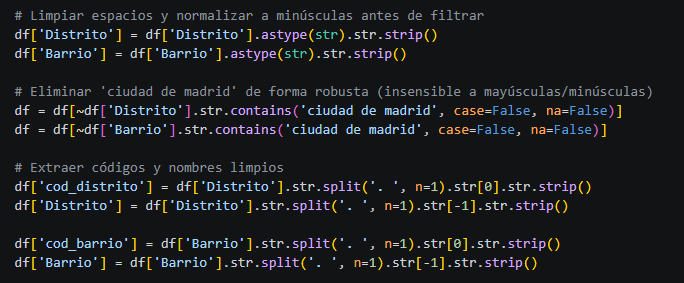
\includegraphics[width=0.75\linewidth]{img/5_3_2_eliminar_madrid.png}
\caption{Lógica implementada para la exclusión del registro municipal consolidado y duplicados distritales.}
\label{fig:clean_aggregates}
\end{figure}

\subsection{Normalización Unicode NFC y Corrección de Encoding}
Debido a la diversidad de plataformas en las que se generan los archivos CSV municipales originales de Madrid, se detectó un severo conflicto de codificación de caracteres provocado por la lectura incorrecta de ficheros codificados en UTF-8 con firmas y acentos españoles bajo el estándar de almacenamiento Latin-1 (ISO-8859-1). Esto generaba la corrupción sistemática de nombres de zonas administrativas históricas de Madrid (por ejemplo, \textit{``Chamberí''} en lugar de \textit{``Chamberí''} o \textit{``Vicálvaro''} en lugar de \textit{``Vicálvaro''}). 

Para solucionar este conflicto de manera definitiva, el script aplica una limpieza profunda de cadenas que realiza una normalización Unicode bajo el estándar de forma canónica compatible (NFC, \textit{Normalization Form Canonical Composition}) y aplica un mapa de traducción estricto para recuperar y conservar la ortografía oficial en español:
\begin{align*}
    \text{á} &\rightarrow \text{á} \qquad & \text{é} &\rightarrow \text{é} \\
    \text{í} &\rightarrow \text{í} \qquad & \text{ó} &\rightarrow \text{ó} \\
    \text{ú} &\rightarrow \text{ú} \qquad & \text{ñ} &\rightarrow \text{ñ} \\
    \text{ù} &\rightarrow \text{ñ} \qquad & \text{Â} &\rightarrow \text{[espacio vacío]}
\end{align*}
Adicionalmente, se implementa una lógica de parseo administrativo para nombres que incorporan prefijos numéricos de ordenamiento oficial (como \textit{``01. Centro''}), para lo cual se aplica un divisor estricto mediante la subcadena \texttt{'. '} que separa el código administrativo (\texttt{cod\_distrito = '01'}) para usarlo como clave primaria relacional de tipo entero; esto aísla el nombre textual limpio (\texttt{Distrito = 'Centro'}) de modo que quede libre de interferencias de indexación.

\subsection{Lógica de Imputaciones Espacial y Temporal}
La consistencia analítica del DataMart exige la ausencia de valores nulos o vacíos (\textit{NaN}) en variables físicas estructurales como la superficie media. Sin embargo, el archivo bruto municipal de superficies presentaba dos problemas críticos de vacíos: barrios de reciente creación o baja densidad (como Valderribas) que carecían de registros consolidados, y la total ausencia de datos de superficie para el año en curso (2026) debido al ciclo habitual de retraso en las publicaciones oficiales. 

Para resolver estas limitaciones sin introducir distorsiones estadísticas ficticias, el script implementa un módulo de imputación multiescala avanzado:
\begin{itemize}
    \item \textbf{Imputación espacial por vecindad:} Los nulos geográficos puntuales de superficie media en un barrio se imputan dinámicamente mediante el cálculo de la media ponderada del resto de los barrios pertenecientes a su mismo distrito administrativo:
    $$\text{superficie\_media}_{(\text{barrio\_nulo})} = \frac{1}{N} \sum_{i=1}^{N} \text{superficie\_media}_{(\text{barrios\_del\_distrito})}$$
    \item \textbf{Imputación temporal por media móvil proyectada:} Para resolver la brecha temporal del año 2026, el script ejecuta una imputación basada en la media móvil de los registros consolidados más recientes de cada barrio correspondientes a los años 2023, 2024 y 2025:
    $$\text{superficie\_media}_{(barrio, 2026)} = \frac{1}{3} \sum_{t=2023}^{2025} \text{superficie\_media}_{(barrio, t)}$$
    Esta imputación temporal asegura que las simulaciones financieras mantengan la consistencia edificatoria de la capital sin alterar la estructura histórica real del suelo urbano.
\end{itemize}

\begin{figure}[H]
\centering
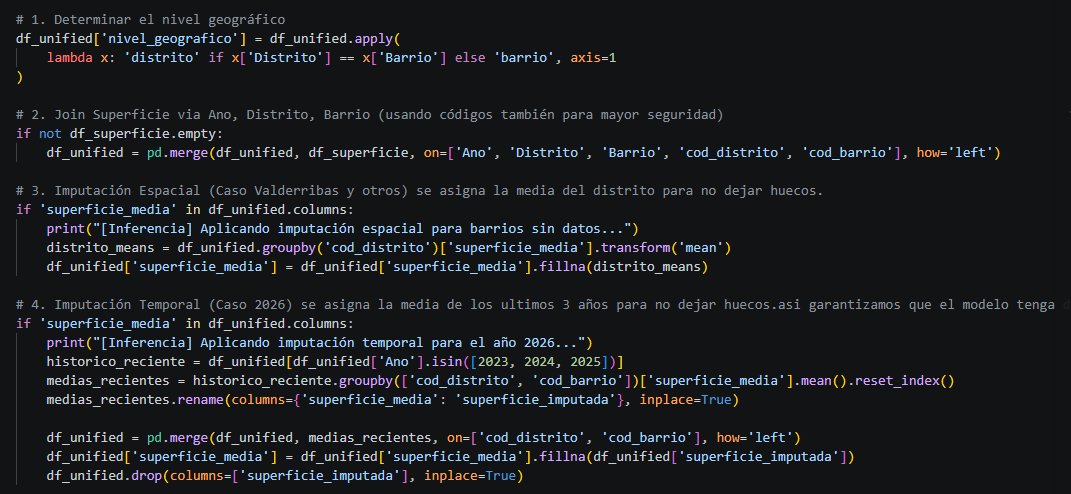
\includegraphics[width=0.85\linewidth]{img/5.3.4 img.png}
\caption{Código fuente que detalla las técnicas de imputación por vecindad espacial y proyección temporal de la superficie media.}
\label{fig:imputations_code}
\end{figure}

\subsection{Corte Temporal de Seguridad y Control de \textit{Ghost Data}}
En el ámbito predictivo, un riesgo severo es el sesgo de filtración de futuro (\textit{data leakage}), que se produce cuando los modelos de inteligencia artificial se entrenan accidentalmente con datos imputados o extrapolados que pertenecen a períodos futuros que aún no han ocurrido en el mercado real. 

Dado que la fecha del sistema analítico real se fija en el 30 de mayo de 2026, y el último mes con registros transaccionales oficiales completos y cerrados es abril de 2026, el script implementa un filtro de corte de seguridad estricto que elimina de forma automática cualquier registro temporal que supere el identificador límite \texttt{current\_time\_limit = 202604}. Esta directriz garantiza la pureza del DataMart y delega de manera exclusiva en los modelos supervisados de Machine Learning la tarea de estimar y proyectar los precios inmobiliarios a partir de mayo de 2026, lo que elimina por completo la interferencia de datos ficticios en el sistema.

\subsection{Integración Socioeconómica y Macroeconómica}
La fase de transformación unifica el contexto socioeconómico y financiero al cruzar los registros residenciales con las variables externas:
\begin{itemize}
    \item \textbf{Mapeo de Renta Media disponible por Hogar:} Se procesa el archivo bruto de renta disponible de la Fase 5 (\textit{renta\_media.csv}), para lo cual aísla mediante un parseador jerárquico el código normalizado de barrio para inyectarlo como un atributo estructural en la dimensión espacial (\textit{Dim\_Barrio}); esto dota al sistema de la variable explicativa del poder adquisitivo.
    \item \textbf{Integración del volumen de transacciones registrales:} El script lee las compraventas reales del Colegio de Registradores (\textit{transactions\_clean.csv}), las cuales se mapean con base en el año de operación e identificador de distrito para incorporarlas como la columna \textit{num\_transacciones} en la tabla de hechos de operaciones; esto proporciona la métrica clave de liquidez.
    \item \textbf{Carga de la tabla macroeconómica de hechos comunes:} Se lee el histórico mensual del Euríbor a un año y los tipos de interés del Banco de España, publicados en el Portal de Datos Abiertos del Ayuntamiento de Madrid (Código~0504020100150), y se mapean en relación con el código temporal de mes y año (\textit{id\_tiempo}) en la tabla de hechos compartida \textit{Fact\_Economica}; de esta manera, se completa el espectro financiero que impacta en el acceso a la hipoteca media.
\end{itemize}

\subsection{Formulación e Inyección del Indicador de Rentabilidad (Yield)}
El indicador analítico por excelencia en la toma de decisiones de inversión inmobiliaria es la Rentabilidad Bruta Anual (Yield). Tradicionalmente, este indicador se calcula de forma aislada y estática. En esta infraestructura, se ha desarrollado el script especializado \textit{calc\_yield.py} que calcula y actualiza dinámicamente este valor para cada corte temporal y espacial de la base de datos analítica.

Para formular el Yield, el script realiza en primer lugar una agrupación y pivotado de la tabla analítica unificada, de forma que el precio de venta por metro cuadrado y el precio de alquiler por metro cuadrado se consolidan como columnas independientes para una misma observación de año, mes, distrito y barrio. Una vez aplanada la estructura, y tras aplicar una regla de seguridad que sustituye los valores nulos o iguales a cero en el precio de venta por valores vacíos para prevenir errores fatales de división por cero, se aplica la fórmula matemática estándar de economía urbana:
$$\text{Yield}_{(barrio, mes, anio)} = \frac{\text{Precio\_m2\_alquiler}_{(barrio, mes, anio)} \times 12}{\text{Precio\_m2\_venta}_{(barrio, mes, anio)}}$$
El resultado obtenido, expresado en formato decimal de alta precisión (redondeado a cuatro decimales), se inyecta nuevamente de forma masiva en la tabla de hechos del DataMart físico relacional mediante la ejecución del módulo de persistencia parametrizado. Esta inyección secuencial se ilustra de manera detallada en las siguientes capturas del código de inyección:

\begin{figure}[H]
\centering
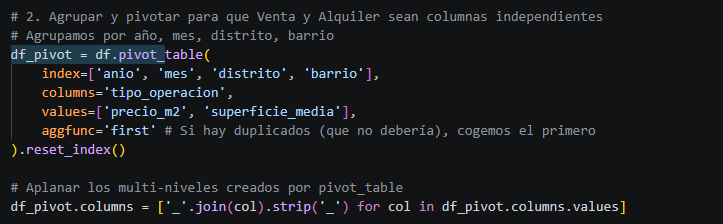
\includegraphics[width=0.75\linewidth]{img/5.3.7.1.png}
\caption{Agrupación y pivotado matricial de precios de venta y alquiler para consolidarlos como columnas independientes por barrio y período temporal.}
\label{fig:yield_calc_1}
\end{figure}

\begin{figure}[H]
\centering
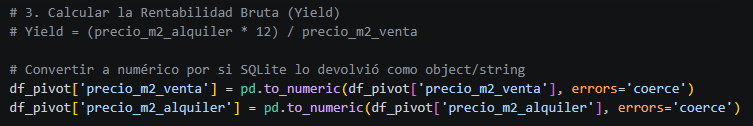
\includegraphics[width=0.85\linewidth]{img/5.3.7.2.png}
\caption{Conversión explícita a tipo numérico de las variables de precio de venta y alquiler como paso previo al cálculo del indicador de rentabilidad.}
\label{fig:yield_calc_2}
\end{figure}

\begin{figure}[H]
\centering
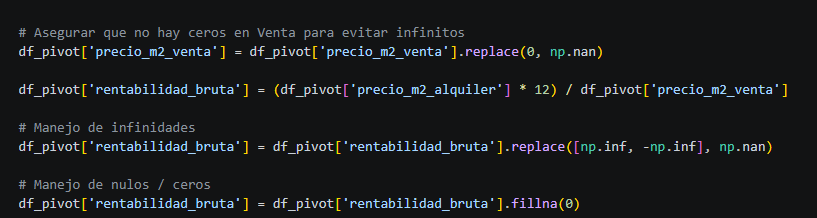
\includegraphics[width=0.85\linewidth]{img/5.3.7.3.png}
\caption{Cálculo del Yield bruto anual, reemplazo de ceros para evitar divisiones por infinito y limpieza de valores nulos en el resultado final.}
\label{fig:yield_calc_3}
\end{figure}

\begin{figure}[H]
\centering
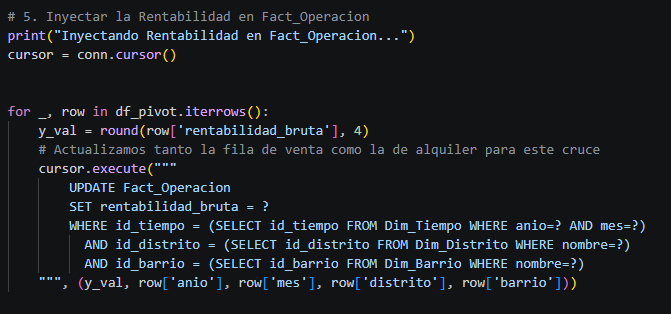
\includegraphics[width=0.70\linewidth]{img/5.3.7.4.png}
\caption{Inyección paramétrica y secuencial del Yield calculado en la tabla de hechos Fact\_Operacion mediante consultas SQL parametrizadas.}
\label{fig:yield_calc_4}
\end{figure}

Esta inyección bidireccional garantiza que tanto el registro de venta como el de alquiler cuenten con el indicador de rentabilidad asociado al barrio para ese mes específico, lo que hace posibles simulaciones analíticas complejas en tiempo real.

\section{Fase de Carga e Ingesta Relacional (Load)}
Una vez normalizados y transformados los datos en la memoria intermedia de Python, la etapa final consiste en poblar de forma física y estructurada el DataMart relacional basado en el motor de almacenamiento de baja latencia SQLite. Para este fin, el script de ingesta relacional \textit{ingest\_db.py} orquesta las transacciones y respeta estrictamente las dependencias de claves foráneas e integridad referencial del modelo dimensional diseñado.

El script inicia el flujo mediante la ejecución del archivo lógico de esquema definitivo (\textit{schema\_final.sql}, anteriormente denominado \textit{schema\_2.sql} durante el desarrollo) que limpia el repositorio analítico e inicializa la estructura de tablas e índices del modelo de constelación. A continuación, se ejecutan las inserciones relacionales masivas (\textit{bulk inserts}) bajo el siguiente orden secuencial y lógico de precedencia para evitar violaciones de clave foránea:
\begin{enumerate}
    \item \textbf{Dim\_Tiempo:} Se pueblan las claves temporales generadas dinámicamente con desglose de año, mes y trimestre.
    \item \textbf{Dim\_Distrito:} Se insertan las dimensiones de nivel superior, etapa en la que se estima e inyecta la superficie media distrital agregada.
    \item \textbf{Dim\_Barrio (Capa Especial e Integridad):} Primero se realiza la inserción obligatoria del registro de control de id especial \texttt{id\_barrio = -1} (\textit{``[DATO A NIVEL DISTRITO]''}), y se inicializan sus variables de densidad a cero para permitir uniones de hechos a nivel de distrito. Posteriormente, se realiza la ingesta relacional de los 131 barrios oficiales enriquecidos con su renta media correspondiente, mediante el mapeo de la clave externa \texttt{id\_distrito} con la dimensión de distrito previamente poblada.
    \item \textbf{Fact\_Operacion y Fact\_Economica:} Una vez garantizada la presencia física de todas las dimensiones, se realiza la carga simultánea de las dos tablas de hechos. La tabla \textit{Fact\_Operacion} mapea las claves externas de tiempo, distrito y barrio (con la redirección de los resúmenes distritales al ID -1) e inyecta la métrica registral de volumen de transacciones, mientras que \textit{Fact\_Economica} centraliza los indicadores financieros.
\end{enumerate}

Para asegurar que las consultas del asistente inteligente NLP y el renderizado interactivo de mapas geoespaciales en React se ejecuten en tiempos inferiores a los 100 milisegundos sin sobrecargar el procesador del sistema, el script crea de forma automática índices de árbol B (\textit{B-Tree Indexes}) sobre las columnas de búsqueda frecuentes del DataMart analítico. Esta arquitectura física asegura tiempos de respuesta inferiores a 100 ms en las consultas del asistente NLP y el renderizado interactivo de mapas.

\begin{figure}[H]
\centering
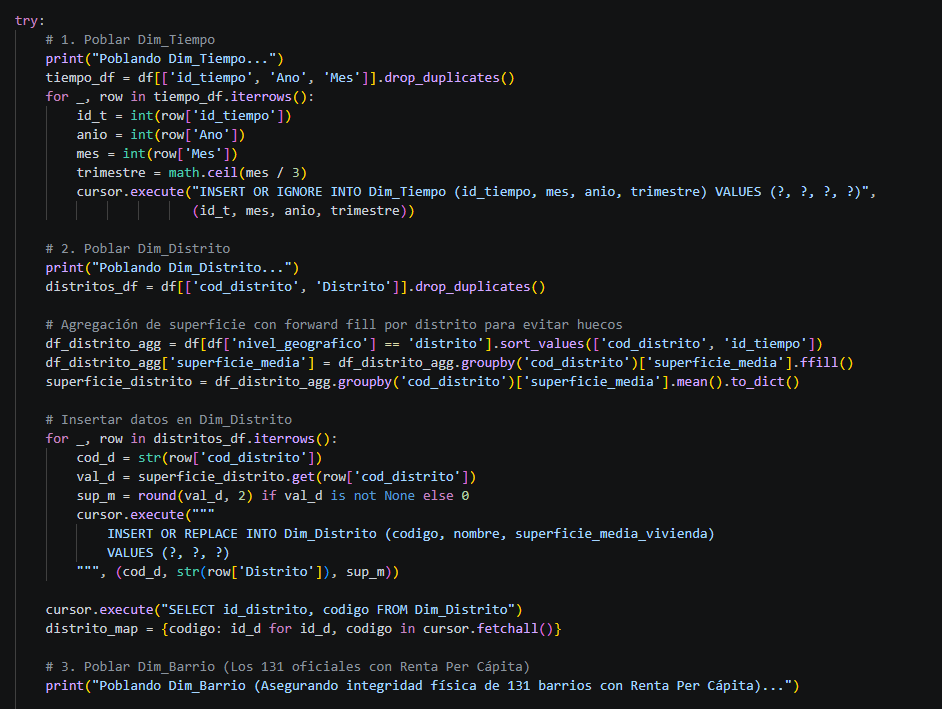
\includegraphics[width=0.85\linewidth]{img/5.4.png}
\caption{Lógica operacional del proceso de carga relacional y construcción secuencial de tablas e índices.}
\label{fig:load_process}
\end{figure}

\section{Enriquecimiento Geoespacial mediante OpenStreetMap}
La ciencia de datos inmobiliaria moderna demuestra que el valor de una vivienda no depende únicamente de sus características físicas internas, sino del entorno urbano en el que se ubica. Para incorporar esta perspectiva espacial en la plataforma, se ha desarrollado un módulo de enriquecimiento multiescalar basado en la extracción e indexación de datos geográficos de OpenStreetMap mediante las librerías científicas especializadas \textit{OSMnx} (Boeing, 2017) y \textit{GeoPandas} en Python.

\subsection{Geocodificación y Extracción de Polígonos de Barrios}
El primer paso del proceso, implementado en \textit{calc\_spatial\_features.py}, consiste en extraer los polígonos fronterizos reales de los 131 barrios de Madrid. Para ello, se formula una geocodificación robusta programática que consulta la API de OpenStreetMap mediante la función \texttt{ox.geocode\_to\_gdf}. 

Para evitar fallas de geocodificación debidas a acentos o nomenclaturas administrativas particulares en español, se implementó un sistema de reintento o desbordamiento en cascada: el script inicia la búsqueda en base a la cadena \texttt{'\{Nombre\_Barrio\}, Madrid, Spain'}; si la petición no devuelve resultados, se ejecuta una consulta con el filtro geográfico redundante de su demarcación superior \texttt{'\{Nombre\_Barrio\}, \{Nombre\_Distrito\}, Madrid, Spain'}. Los límites geométricos devueltos se consolidan en el archivo cartográfico vectorial unificado en formato GeoJSON \textit{barrios\_polygons.geojson}.

\begin{figure}[H]
\centering
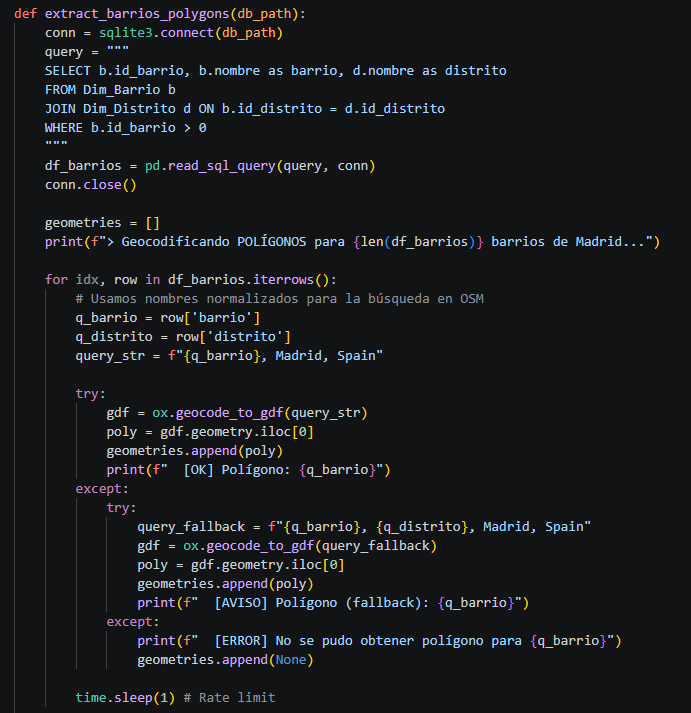
\includegraphics[width=0.70\linewidth]{img/5.5.1.png}
\caption{Implementación del script calc\_spatial\_features.py para la geocodificación de barrios e interconexión a OpenStreetMap.}
\label{fig:geocoding_code}
\end{figure}

\subsection{Métricas de Densidad Multiescalar y Distancia al Kilómetro Cero}
Una vez establecidos los límites geométricos de cada barrio, se ejecuta una consulta espacial para recuperar todos los Puntos de Interés (POIs) y nodos de infraestructura urbana de la capital. Estos puntos se clasifican jerárquicamente en categorías de contexto urbano (servicios públicos esenciales como escuelas y universidades; salud y hospitales generales; transporte y movilidad urbana; comercio y supermercados; y zonas verdes, parques y ocio urbano). A partir del centroide geométrico representativo de cada polígono de barrio, el script ejecuta un cálculo geoespacial de alta complejidad técnica:
\begin{itemize}
    \item \textbf{Cálculo radial del gradiente del centroide (Sol):} Se determina de forma exacta la distancia euclídea proyectada en la cuadrícula UTM de cada barrio al Kilómetro Cero de la capital (Puerta del Sol, ubicado en las coordenadas geográficas de precisión Point \texttt{-3.7038, 40.4168}), lo que permite capturar la influencia de la centralidad residencial:
    $$\text{dist\_to\_sol\_m} = \text{Distancia\_Métrica}(\text{Centroide\_Barrio}, \text{Punto\_Sol})$$
    \item \textbf{Buffers de Densidad Multiescalar:} Para modelar la accesibilidad en base a diferentes hábitos y necesidades residenciales de los usuarios de la plataforma, se computa la densidad o presencia total de equipamientos urbanos bajo tres radios o buffers concéntricos específicos desde el centroide del barrio:
    \begin{itemize}
        \item \textbf{Buffer de 500 metros, 1 kilómetro y 2 kilómetros:} Para la definición detallada y justificación metodológica de los radios de análisis adoptados (5--7~min peatonal, 10--12~min, 20--25~min/5~min en transporte), véase la Sección~\ref{sec:enriquecimiento} del Capítulo~\ref{chap:datos}.
    \end{itemize}
\end{itemize}

\begin{figure}[H]
\centering
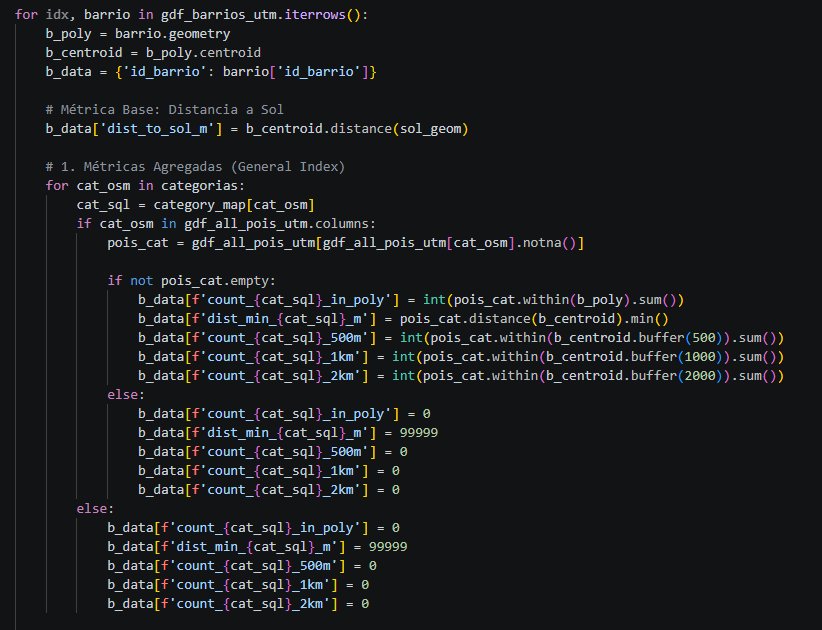
\includegraphics[width=0.80\linewidth]{img/5.5.2.png}
\caption{Algoritmo para el cálculo de distancias al Kilómetro Cero y obtención de buffers multiescala de densidad.}
\label{fig:density_buffers_code}
\end{figure}

\subsection{Técnica de Deduplicación de Paradas e Infraestructuras de Tránsito}
Un problema recurrente en el análisis geoespacial basado en bases de datos abiertas es el sesgo de sobredensidad provocado por la duplicidad de nodos geográficos en OpenStreetMap. Por ejemplo, una misma estación de metro de Madrid cuenta con múltiples bocas de acceso físico digitalizadas como puntos independientes en la base de datos de origen, y una intensidad de tráfico importante puede registrar hasta cuatro paradas de autobús idénticas según el sentido de circulación de la vía. Si no se corrigen estas redundancias, los recuentos de paradas de transporte en los buffers multiescala arrojarían valores artificialmente inflados que sesgarían el entrenamiento de los algoritmos de Machine Learning.

Para solventar esta anomalía espacial, se diseñó e implementó una técnica de deduplicación y disolución espacial basada en métricas físicas reales:
\begin{enumerate}
    \item \textbf{Proyección UTM:} Las coordenadas espaciales originales en grados decimales (WGS84, EPSG:4326) se proyectan al huso métrico correspondiente a Madrid (UTM 30N, EPSG:32630) para realizar cálculos en unidades de distancia reales (metros).
    \item \textbf{Búfer de amortiguación de proximidad:} Se aplica a todos los nodos de transporte (estaciones de metro y paradas de autobús) un buffer circular de amortiguación con un radio físico estricto de \textbf{150 metros}.
    \item \textbf{Disolución por agrupamiento semántico:} El script ejecuta una disolución espacial el cual combina los polígonos circulares resultantes que comparten el mismo atributo nominal de parada (\texttt{dissolve(by='name')}). Este paso fusiona los accesos múltiples e independientes de una estación en un único polígono continuo representativo.
    \item \textbf{Centroide de la estación disuelta:} A partir de la geometría unificada resultante, el script calcula el centroide geométrico del polígono disuelto para actuar como el único punto representativo del nodo de transporte deduplicado.
    \item \textbf{Conversión a formato de origen:} Las geometrías resultantes se convierten de nuevo a coordenadas de grados decimales (WGS84) para su correcto guardado en el archivo GeoJSON analítico consolidado.
\end{enumerate}
Esta técnica de deduplicación asegura que la densidad espacial calculada en los buffers de la dimensión espacial represente fielmente la infraestructura urbana de la capital, sin inflación artificial por nodos duplicados.

\section{Orquestación y Validación Analítica del Pipeline}
La robustez y reproducibilidad científica del pipeline de ingeniería de datos se fundamentan en su capacidad de orquestación centralizada y en sus módulos de validación estricta, que aseguran que el flujo opere de principio a fin de manera autónoma bajo controles de calidad sistemáticos.

\subsection{El Pipeline Maestro de Datos (master\_run\_pipeline.py)}
Para coordinar secuencialmente la ejecución de todas las fases descritas, se ha desarrollado el script maestro de orquestación de datos \textit{master\_run\_pipeline.py} en Python. El orquestador opera mediante una arquitectura de subprocesos dinámicos en cascada que emplea la librería \textit{subprocess}. El flujo maestro ejecuta secuencialmente las siguientes fases metodológicas:
\begin{figure}[H]
\centering
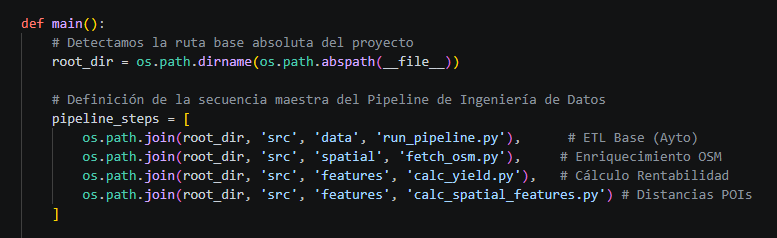
\includegraphics[width=0.67\linewidth]{img/5.6.1.0.png}
\caption{Definición de las etapas secuenciales del pipeline de datos en el script orquestador maestro.}
\label{fig:pipeline_steps_code}
\end{figure}

\begin{figure}[H]
\centering
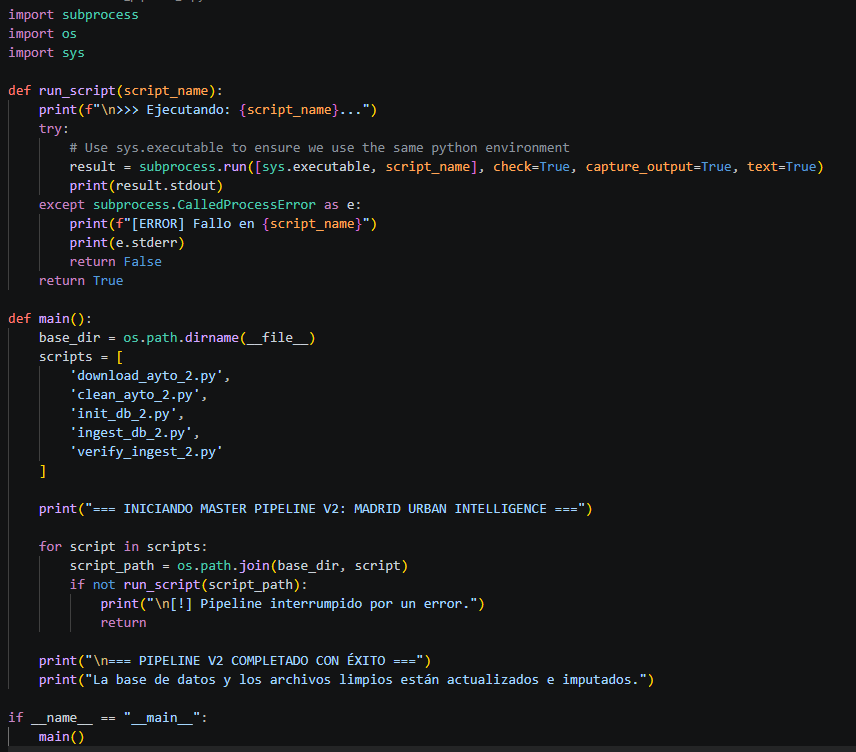
\includegraphics[width=0.63\linewidth]{img/5.6.1.png}
\caption{Orquestador maestro master\_run\_pipeline.py para la automatización secuencial y control de excepciones del pipeline analítico.}
\label{fig:orchestrator_code}
\end{figure}
El script realiza un control de ejecución y hereda de forma dinámica las variables y ruta del entorno operativo del usuario mediante la llamada a \texttt{sys.executable}, lo que garantiza que cualquier fallo sintáctico o de conexión en una fase específica detenga de inmediato el flujo global mediante un mecanismo de captura y registro de excepciones. Este comportamiento previene que se ingesten datos incompletos en el Datamart final o se alimenten modelos de predicción con series temporales corruptas.

\subsection{Script de Verificación y Auditoría de Datos (verificar\_datos.py)}
Para asegurar la integridad analítica del DataMart una vez completada la ejecución del orquestador maestro, se diseñó e implementó el script de verificación y auditoría \textit{verificar\_datos.py}. Este script realiza una inspección física y relacional del archivo de base de datos SQLite resultante (\textit{madrid\_intelligence.db}), con el fin de ejecutar las siguientes tareas de control:
\begin{itemize}
    \item \textbf{Conteo del censo relacional:} Valida la presencia física y el volumen de registros insertados en las cuatro tablas principales para contrastar la completitud de la base de datos (conteo de `Dim\_Tiempo`, `Dim\_Distrito`, `Dim\_Barrio` y `Fact\_Operacion`).
    \item \textbf{Auditoría de Granularidad Espacial:} Ejecuta una consulta analítica de agrupación para verificar la distribución y separación estricta de los hechos a nivel de barrio y de distrito (redirigidos a id -1), tal como se ilustra en la Figura~\ref{fig:spatial_granularity_audit}.
\begin{figure}[H]
\centering
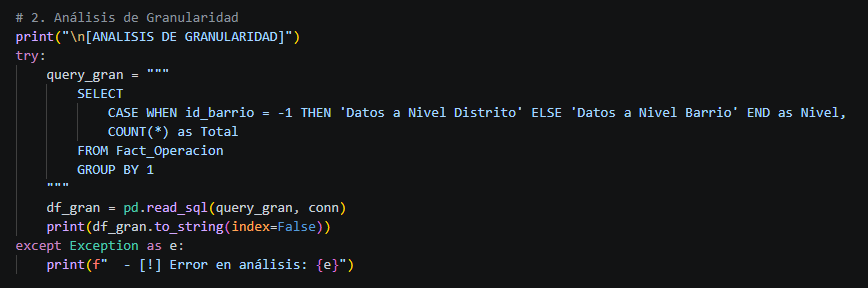
\includegraphics[width=0.80\linewidth]{img/5.6.2.png}
\caption{Consulta analítica de verificación y auditoría de la granularidad espacial a nivel de barrio y distrito.}
\label{fig:spatial_granularity_audit}
\end{figure}
    \item \textbf{Validación de Cobertura Espacial OSMnx:} Inspecciona que los barrios registrados en \textit{Dim\_Barrio} presenten su geocodificación y gradiente euclídeo al Kilómetro Cero (\textit{dist\_to\_sol\_m}) de forma completa y variada; asimismo, se comprueba que el registro especial distrital `-1` tenga inicializadas a cero todas sus variables de densidad multiescalar.
    \item \textbf{Muestra de transacciones e inyección de Yield:} Realiza una consulta con uniones relacionales múltiples para presentar los últimos 5 registros detectados de la tabla de hechos, con el objetivo de auditar visualmente que los campos de variación mensual y rentabilidad bruta anual (\textit{rentabilidad\_bruta}) muestren valores coherentes.
\end{itemize}

\subsection{Auditoría de Optimización Relacional e Indexada (verify\_indices.py)}
Finalmente, para contrastar empíricamente que los índices analíticos compuestos de árbol B creados durante la fase de carga operan de forma activa y garantizan la sub-latencia de respuesta en las interfaces visuales y en las consultas conversacionales NLP, se ha desarrollado el script de auditoría de rendimiento \textit{verify\_indices.py}.

El script se conecta al DataMart físico y ejecuta análisis de optimización relacional sobre consultas de joins complejas mediante la sentencia explícita de SQLite \texttt{EXPLAIN QUERY PLAN}. Al auditar consultas que filtran por nombre de barrio o que unen la tabla de hechos con las dimensiones espaciales para analizar rentabilidades, el script captura el plan de ejecución lógico del optimizador de la base de datos. Esto ayuda a certificar mediante trazas técnicas si el motor recurre a un escaneo completo de la tabla (\textit{SCAN TABLE}, ineficiente) o si aprovecha de forma óptima la indexación de árbol B para realizar búsquedas directas con base en claves primarias y foráneas (\textit{SEARCH TABLE USING INDEX}, óptimo), lo que certifica la reducción de tiempos de procesamiento relacional y la eficiencia del diseño dimensional de la infraestructura.


% --- Capítulo 6: Modelado Predictivo y Selección de Algoritmos ---
\chapter{Modelado Predictivo y Selección de Algoritmos}
\label{chap:predictive_modeling}
La capacidad de modelar y proyectar de manera sólida las tendencias del mercado inmobiliario descansa en el núcleo analítico de la plataforma \textit{Madrid Urban Intelligent} las tendencias del mercado inmobiliario en la capital. La estimación de precios del suelo urbano no es una tarea de regresión genérica: está sujeta a grandes diferencias de precios entre barrios y a cambios repentinos tanto en la economía como en el tiempo. En este capítulo se expone de forma detallada la experimentación científica y el diseño de la arquitectura predictiva implementada, dividida en varias etapas comparativas de modelos base y una última fase de optimización con la arquitectura definitiva del modelo.

\section{Fase Comparativa: Entrenamiento de Modelos Base}
\label{sec:fase_comparativa}
Para establecer una referencia de partida rigurosa y auditable, la primera etapa de la investigación se centró en evaluar el rendimiento de cuatro algoritmos de aprendizaje automático ampliamente reconocidos en la literatura científica: Random Forest, CatBoost, XGBoost y LightGBM. En esta fase experimental, los modelos se entrenaron con el conjunto de datos residenciales base de origen municipal (precios y superficies de venta y alquiler por zona y periodo) junto con las características espaciales y de equipamiento urbano extraídas de OpenStreetMap (como la distancia al Kilómetro Cero en Sol y la concentración de servicios en buffers radiales), con el fin de evaluar la capacidad de los modelos para estimar los precios basándose únicamente en las características físicas y la localización urbana, bajo la hipótesis de que las zonas con mayor densidad de servicios y proximidad al centro de la capital registrarían estimaciones más exactas o explicarían mejor el precio de la vivienda en esos barrios o distritos.

Para garantizar la reproducibilidad y la imparcialidad científica de la comparativa, se adoptó una validación temporal (\textit{temporal split}): los datos hasta 2025 se emplean como conjunto de entrenamiento y los meses de 2026 como conjunto ciego de test. Esta elección es metodológicamente superior a la validación cruzada espacial k-fold clásica, ya que los datos inmobiliarios presentan alta autocorrelación temporal y el uso de observaciones futuras en el entrenamiento introducía \textit{data leakage}. Todos los modelos fueron configurados con los hiperparámetros por defecto establecidos en las implementaciones de referencia de cada algoritmo: 300 estimadores, tasa de aprendizaje de 0,05 y profundidad máxima de 6; estos valores son los predefinidos en las librerías oficiales de XGBoost (\texttt{max\_depth=6}, Chen \& Guestrin, 2016), LightGBM (\texttt{num\_leaves=31}, Ke et al., 2017), CatBoost (\texttt{depth=6}, Prokhorenkova et al., 2018) y Random Forest (\texttt{max\_depth=None} o sin límite de profundidad, Breiman, 2001); cabe señalar que este último carece de parada temprana (\textit{early stopping}) al tratarse de un ensamble basado en agregación (\textit{bagging}). Esta elección se sustenta en que, como demuestran trabajos fundamentales en el campo como Shwartz-Ziv \& Armon (2022) y Grinsztajn et al. (2022), los algoritmos basados en árboles de decisión superan de manera sistemática a los modelos de Deep Learning (redes neuronales complejas) al trabajar con datos tabulares. Los modelos basados en árboles no solo son más rápidos de entrenar y menos sensibles a los hiperparámetros, sino que capturan de forma nativa las discontinuidades y la naturaleza heterogénea de este tipo de información. Para garantizar una comparación científica e imparcial, todos los modelos se configuraron inicialmente con parámetros uniformes, lo que elimina el sesgo de optimización diferencial y garantiza que las diferencias observadas reflejen exclusivamente la capacidad predictiva intrínseca de cada arquitectura sobre el mismo conjunto de datos, bajo condiciones de igualdad absoluta.

La elección del límite máximo de 300 estimadores (o árboles de decisión) y el diseño de los mecanismos de convergencia temporal responden a dos criterios metodológicos y de optimización fundamentales:
\begin{itemize}
    \item \textbf{Equilibrio entre Cómputo y Precisión:} El análisis de las curvas de aprendizaje en todas las etapas reveló que la práctica totalidad del descenso del error absoluto medio (MAE) y el error cuadrático medio (RMSE) se concentra en los primeros 50 a 100 estimadores. A partir de los 150 árboles, las curvas de pérdida se estabilizan progresivamente hasta quedar planas, demostrando que 300 árboles constituyen un límite superior óptimo para capturar de manera exhaustiva las relaciones no lineales de los datos urbanos. Ampliar el tamaño del ensamble más allá de este umbral (e.g., a 1,000 o 2,000 estimadores) resultaría innecesario, incrementando de forma drástica el tiempo de procesamiento y el coste de cómputo sin aportar ninguna mejora de la precisión, lo que representa un equilibrio ideal entre la precisión del modelo y los recursos de computación necesarios, idóneo para su integración en un entorno de API web en producción.
    \item \textbf{Uniformidad en la Tarea Comparativa:} El establecimiento del mismo límite máximo de 300 estimadores para los cuatro algoritmos (incluyendo una simulación acumulativa de árboles para Random Forest) garantiza un análisis de robustez consistente y libre de variables de control sesgadas, sentando las bases de una comparación científica de rendimiento transparente.
\end{itemize}

\subsection{Modelo Base: Experimentación Inicial}
Para caracterizar de forma exhaustiva el comportamiento predictivo inicial de los cuatro algoritmos seleccionados, se evaluó cada modelo de forma independiente mediante un conjunto de métricas globales y localizadas en distritos con dinámicas de mercado contrastadas: Salamanca (mercado premium de alta gama y precios elevados) y Ciudad Lineal (mercado típico representativo de la capital con alta densidad residencial). La Tabla~\ref{tab:base_model_metrics_venta} y la Tabla~\ref{tab:base_model_metrics_alquiler} detallan la matriz de rendimiento obtenida para los mercados de venta y alquiler, respectivamente.

\begin{table}[H]
\centering
\caption{Matriz de rendimiento comparativa del Escenario Inicial (Modelo Base sin retardo temporal) - Mercado de Venta (€/m\textsuperscript{2})}
\label{tab:base_model_metrics_venta}
\resizebox{\textwidth}{!}{%
\begin{tabular}{|l|c|c|c|c|c|c|c|c|c|c|c|}
\hline
\textbf{Algoritmo} & \textbf{MAE} & \textbf{RMSE} & \textbf{R\textsuperscript{2}} & \textbf{MAPE} & \textbf{Sesgo} & \textbf{MAE} & \textbf{R\textsuperscript{2}} & \textbf{MAE} & \textbf{R\textsuperscript{2}} & \textbf{T. Train} & \textbf{T. Pred} \\
 & \textbf{Global} & \textbf{Global} & \textbf{Global} & \textbf{Global (\%)} & \textbf{Global} & \textbf{Salamanca} & \textbf{Salamanca} & \textbf{C. Lineal} & \textbf{C. Lineal} & \textbf{(s)} & \textbf{(s)} \\
\hline
\textbf{Random Forest} & \textbf{560,92} & \textbf{666,67} & \textbf{0,8966} & \textbf{10,05\%} & \textbf{-487,02} & 645,03 & 0,2954 & \textbf{902,11} & \textbf{0,6372} & 0,486 & 0,063 \\
\textbf{CatBoost} & 844,10 & 894,29 & 0,8139 & 16,10\% & -830,75 & 687,37 & 0,3304 & 1195,34 & 0,3436 & 0,691 & 0,002 \\
\textbf{XGBoost} & 859,63 & 918,72 & 0,8036 & 16,39\% & -840,35 & \textbf{628,90} & \textbf{0,4130} & 1182,98 & 0,3545 & 0,705 & 0,007 \\
\textbf{LightGBM} & 860,80 & 918,40 & 0,8038 & 16,37\% & -844,61 & 656,32 & 0,3715 & 1214,26 & 0,3206 & \textbf{0,351} & \textbf{0,004} \\
\hline
\end{tabular}%
}
\end{table}

\begin{table}[H]
\centering
\caption{Matriz de rendimiento comparativa del Escenario Inicial (Modelo Base sin retardo temporal) - Mercado de Alquiler (€/m\textsuperscript{2})}
\label{tab:base_model_metrics_alquiler}
\resizebox{\textwidth}{!}{%
\begin{tabular}{|l|c|c|c|c|c|c|c|c|c|c|c|}
\hline
\textbf{Algoritmo} & \textbf{MAE} & \textbf{RMSE} & \textbf{R\textsuperscript{2}} & \textbf{MAPE} & \textbf{Sesgo} & \textbf{MAE} & \textbf{R\textsuperscript{2}} & \textbf{MAE} & \textbf{R\textsuperscript{2}} & \textbf{T. Train} & \textbf{T. Pred} \\
 & \textbf{Global} & \textbf{Global} & \textbf{Global} & \textbf{Global (\%)} & \textbf{Global} & \textbf{Salamanca} & \textbf{Salamanca} & \textbf{C. Lineal} & \textbf{C. Lineal} & \textbf{(s)} & \textbf{(s)} \\
\hline
\textbf{Random Forest} & \textbf{1,510} & \textbf{1,739} & \textbf{0,7985} & \textbf{6,99\%} & \textbf{-1,353} & \textbf{1,417} & \textbf{-0,6245} & \textbf{2,008} & \textbf{0,6159} & 0,527 & 0,072 \\
\textbf{CatBoost} & 1,726 & 1,920 & 0,7543 & 8,02\% & -1,714 & 1,873 & -1,5255 & 2,138 & 0,5525 & 0,491 & 0,001 \\
\textbf{XGBoost} & 1,720 & 1,940 & 0,7491 & 8,05\% & -1,711 & 1,735 & -1,2087 & 2,031 & 0,5989 & 0,528 & 0,006 \\
\textbf{LightGBM} & 1,715 & 1,920 & 0,7543 & 8,01\% & -1,705 & 1,688 & -1,1196 & 2,076 & 0,5816 & \textbf{0,190} & \textbf{0,003} \\
\hline
\end{tabular}%
}
\end{table}

El análisis de la matriz de rendimiento revela que todos los modelos entrenados en esta configuración presentan un marcado subajuste generalizado. La ausencia de memoria temporal se traduce en un sesgo global negativo masivo (que oscila entre $-487,02$ y $-844,61$ €/m\textsuperscript{2} en el mercado de venta, y entre $-1,353$ y $-1,705$ €/m\textsuperscript{2} en alquiler), lo que indica que los estimadores subestiman sistemáticamente el valor real del suelo. A nivel de distritos específicos, zonas de gran volatilidad y precios extremos como Salamanca presentan desajustes significativos, llegando incluso a registrar valores de R\textsuperscript{2} negativos en el mercado de alquiler, lo que evidencia la incapacidad de los modelos para capturar las dinámicas de tasación reales sin la inyección de inercias temporales. Los valores de R\textsuperscript{2} negativos observados (como el $-0{,}6245$ en Salamanca alquiler) indican que el modelo predice peor que la media muestral de la variable objetivo, confirmando el fracaso del modelo base en ausencia de memoria temporal. Por otro lado, en términos de eficiencia computacional, LightGBM se posiciona como el algoritmo más rápido tanto en entrenamiento como en inferencia.

Adicionalmente, se generaron las curvas de aprendizaje para auditar la evolución de la pérdida de entrenamiento y validación a lo largo de las iteraciones. Las Figuras~\ref{fig:learning_curves_rf_lgb} y~\ref{fig:learning_curves_xgb_cat} muestran este comportamiento para los cuatro algoritmos. Se observa que mientras Random Forest estabiliza su error de validación de forma temprana debido a su naturaleza basada en bagging, los modelos basados en boosting (LightGBM, XGBoost y CatBoost) experimentan un descenso continuo del gradiente que converge de manera suave a lo largo de los 300 estimadores establecidos, sin indicios de sobreajuste temprano dada la simplicidad del conjunto de datos inicial.

\begin{figure}[H]
\centering
\begin{tabular}{cc}
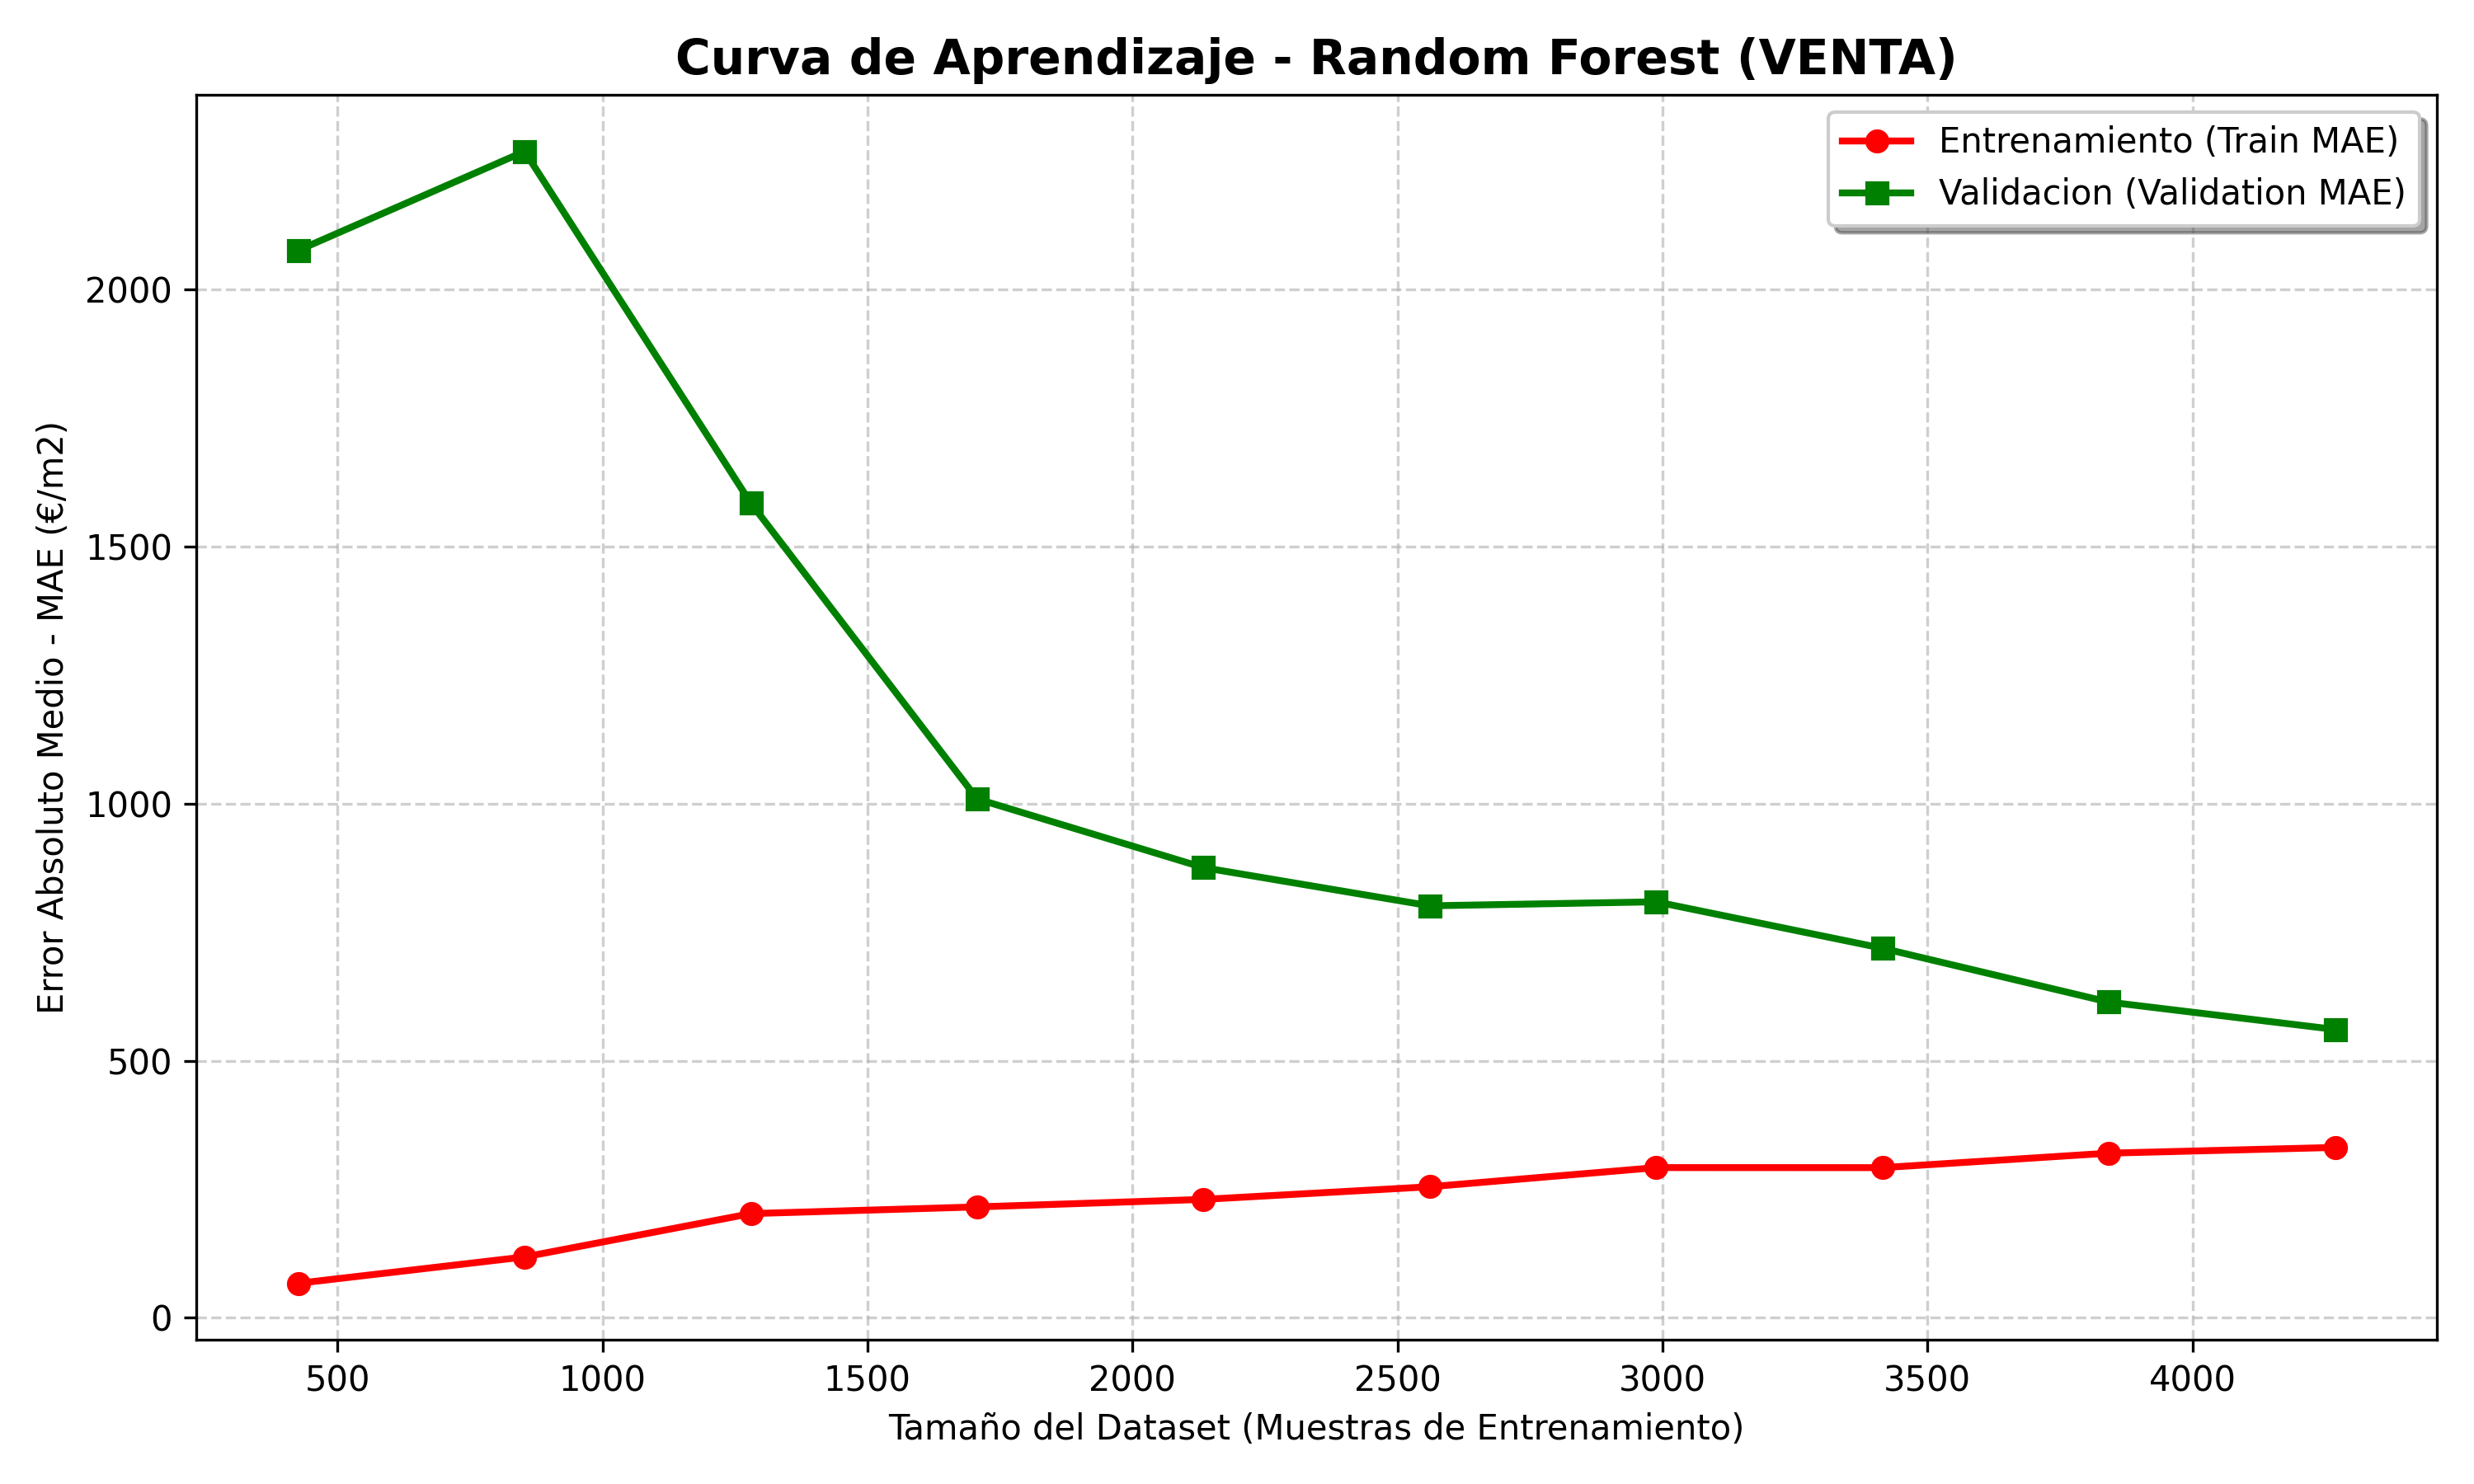
\includegraphics[width=0.40\linewidth]{img/base0_learning_curve_random_forest_venta.png} & 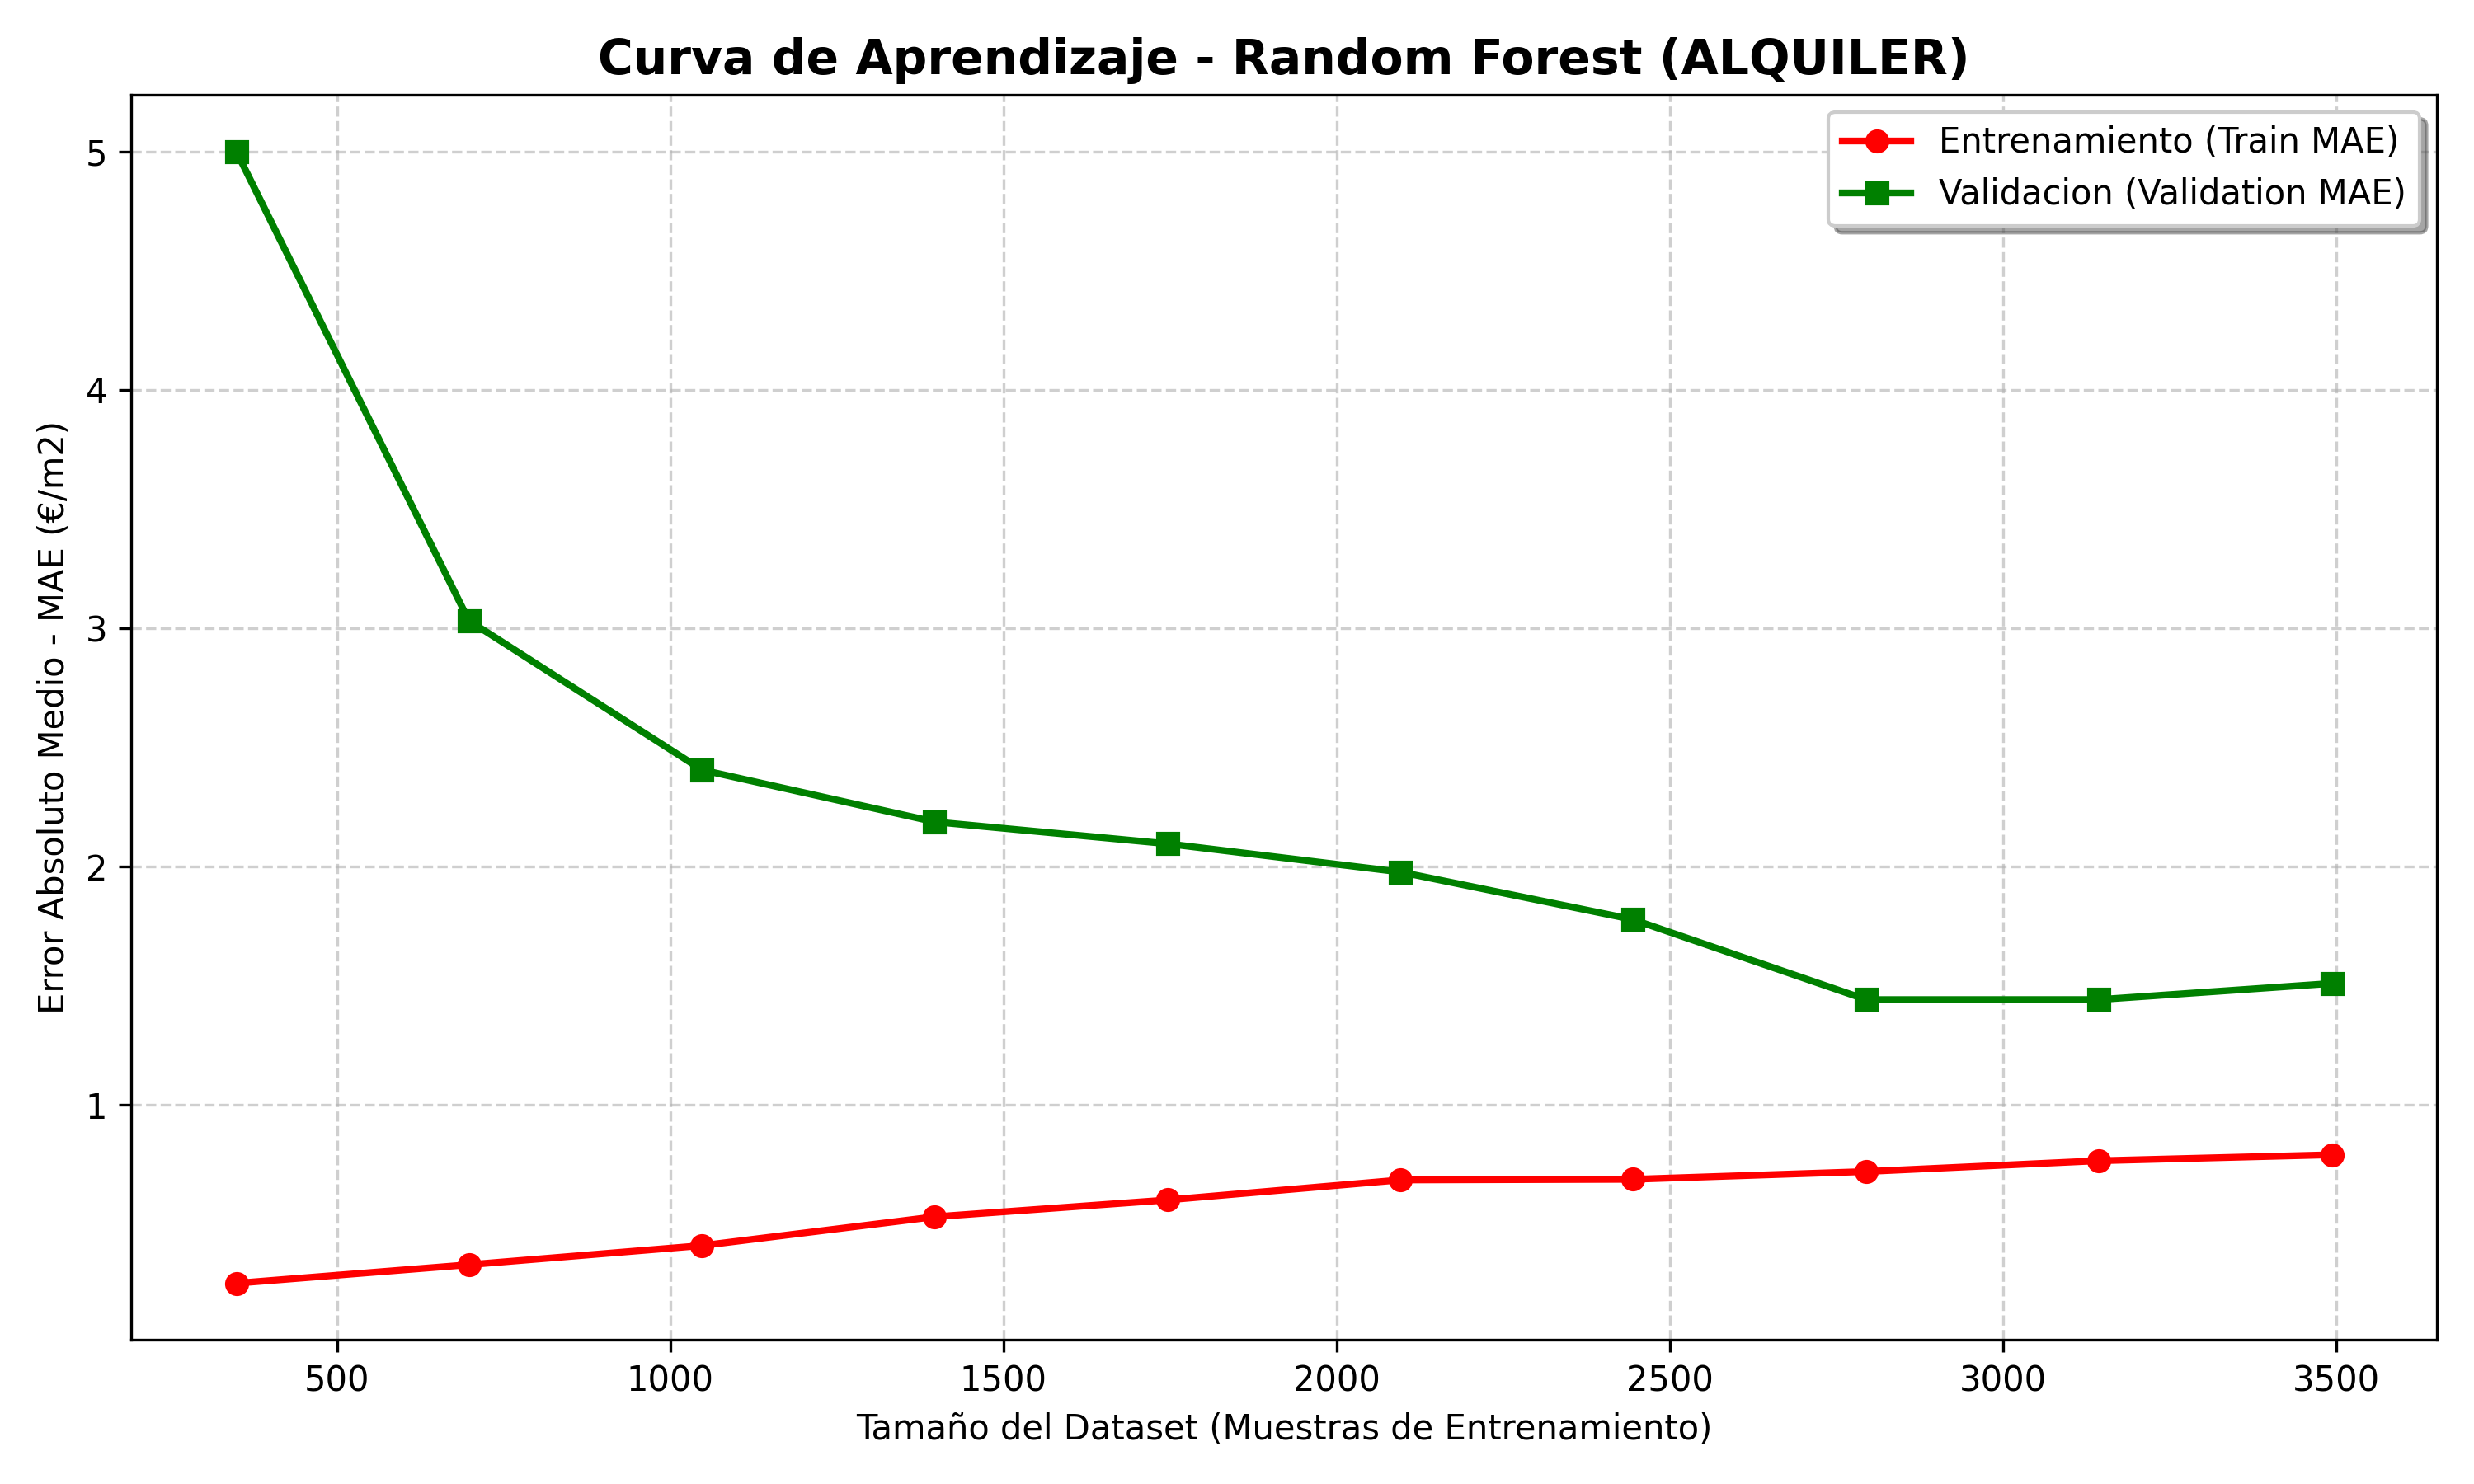
\includegraphics[width=0.40\linewidth]{img/base0_learning_curve_random_forest_alquiler.png} \\
(a) Random Forest - Venta & (b) Random Forest - Alquiler \\
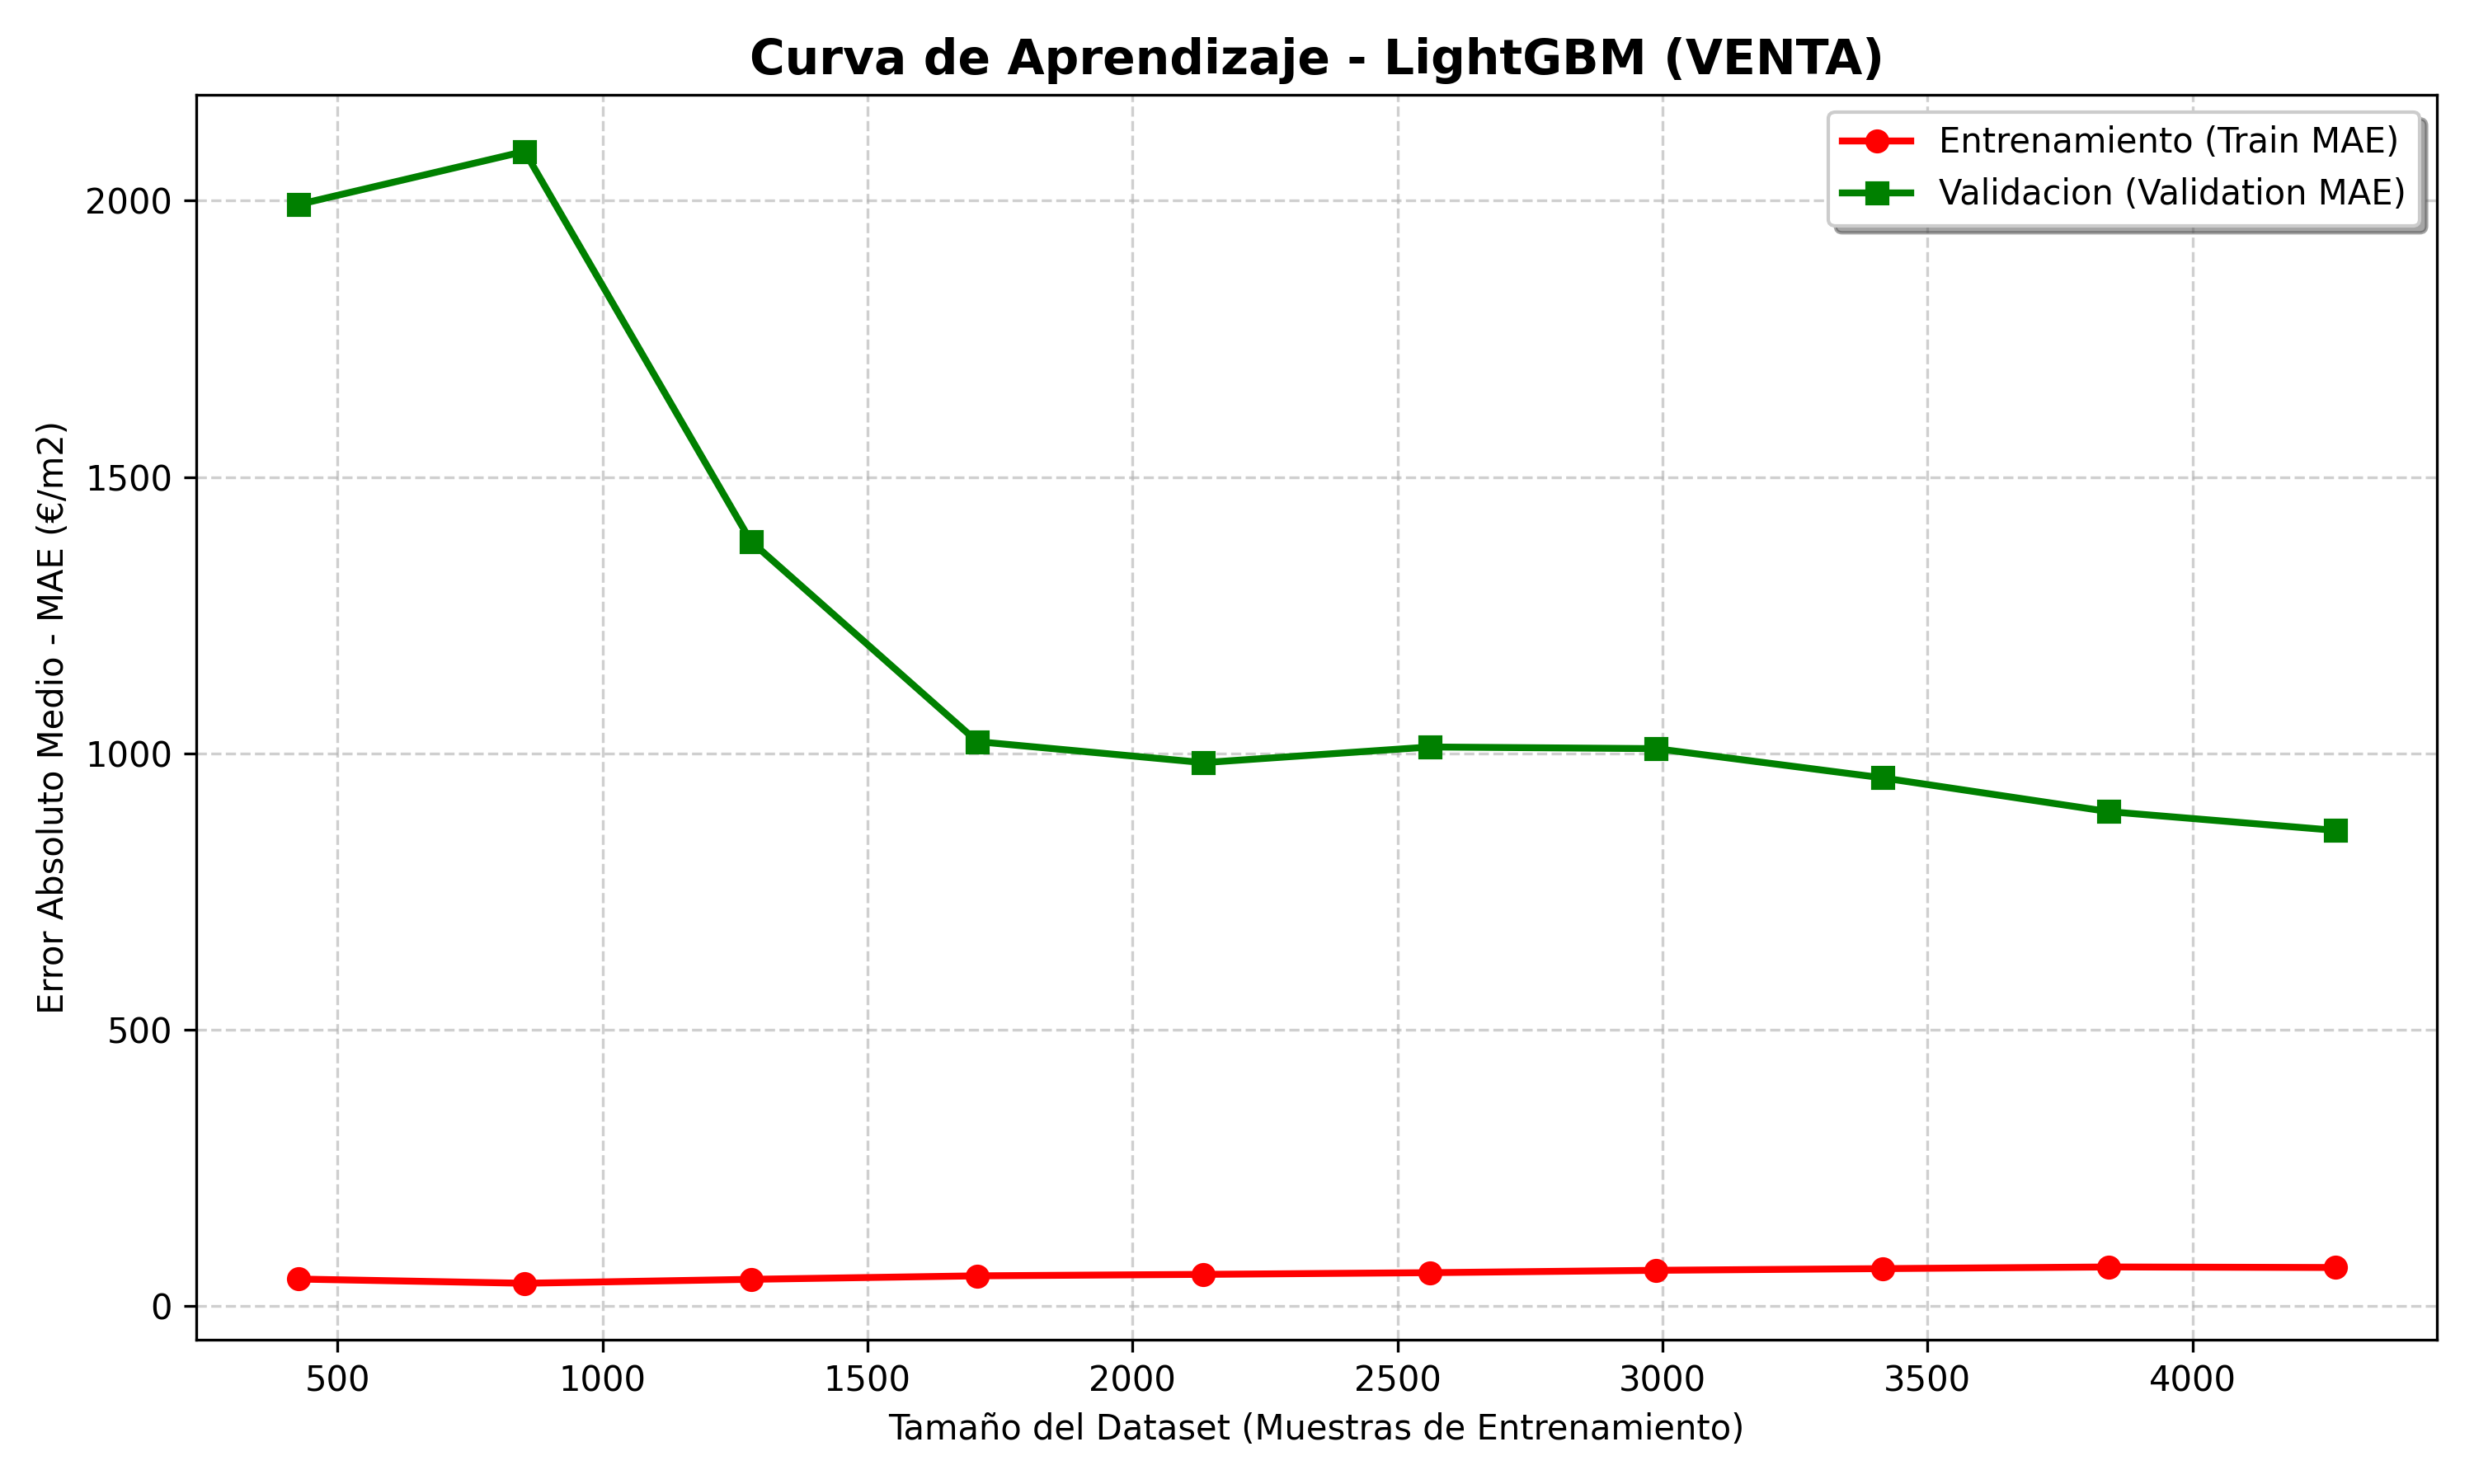
\includegraphics[width=0.40\linewidth]{img/base0_learning_curve_lightgbm_venta.png} & 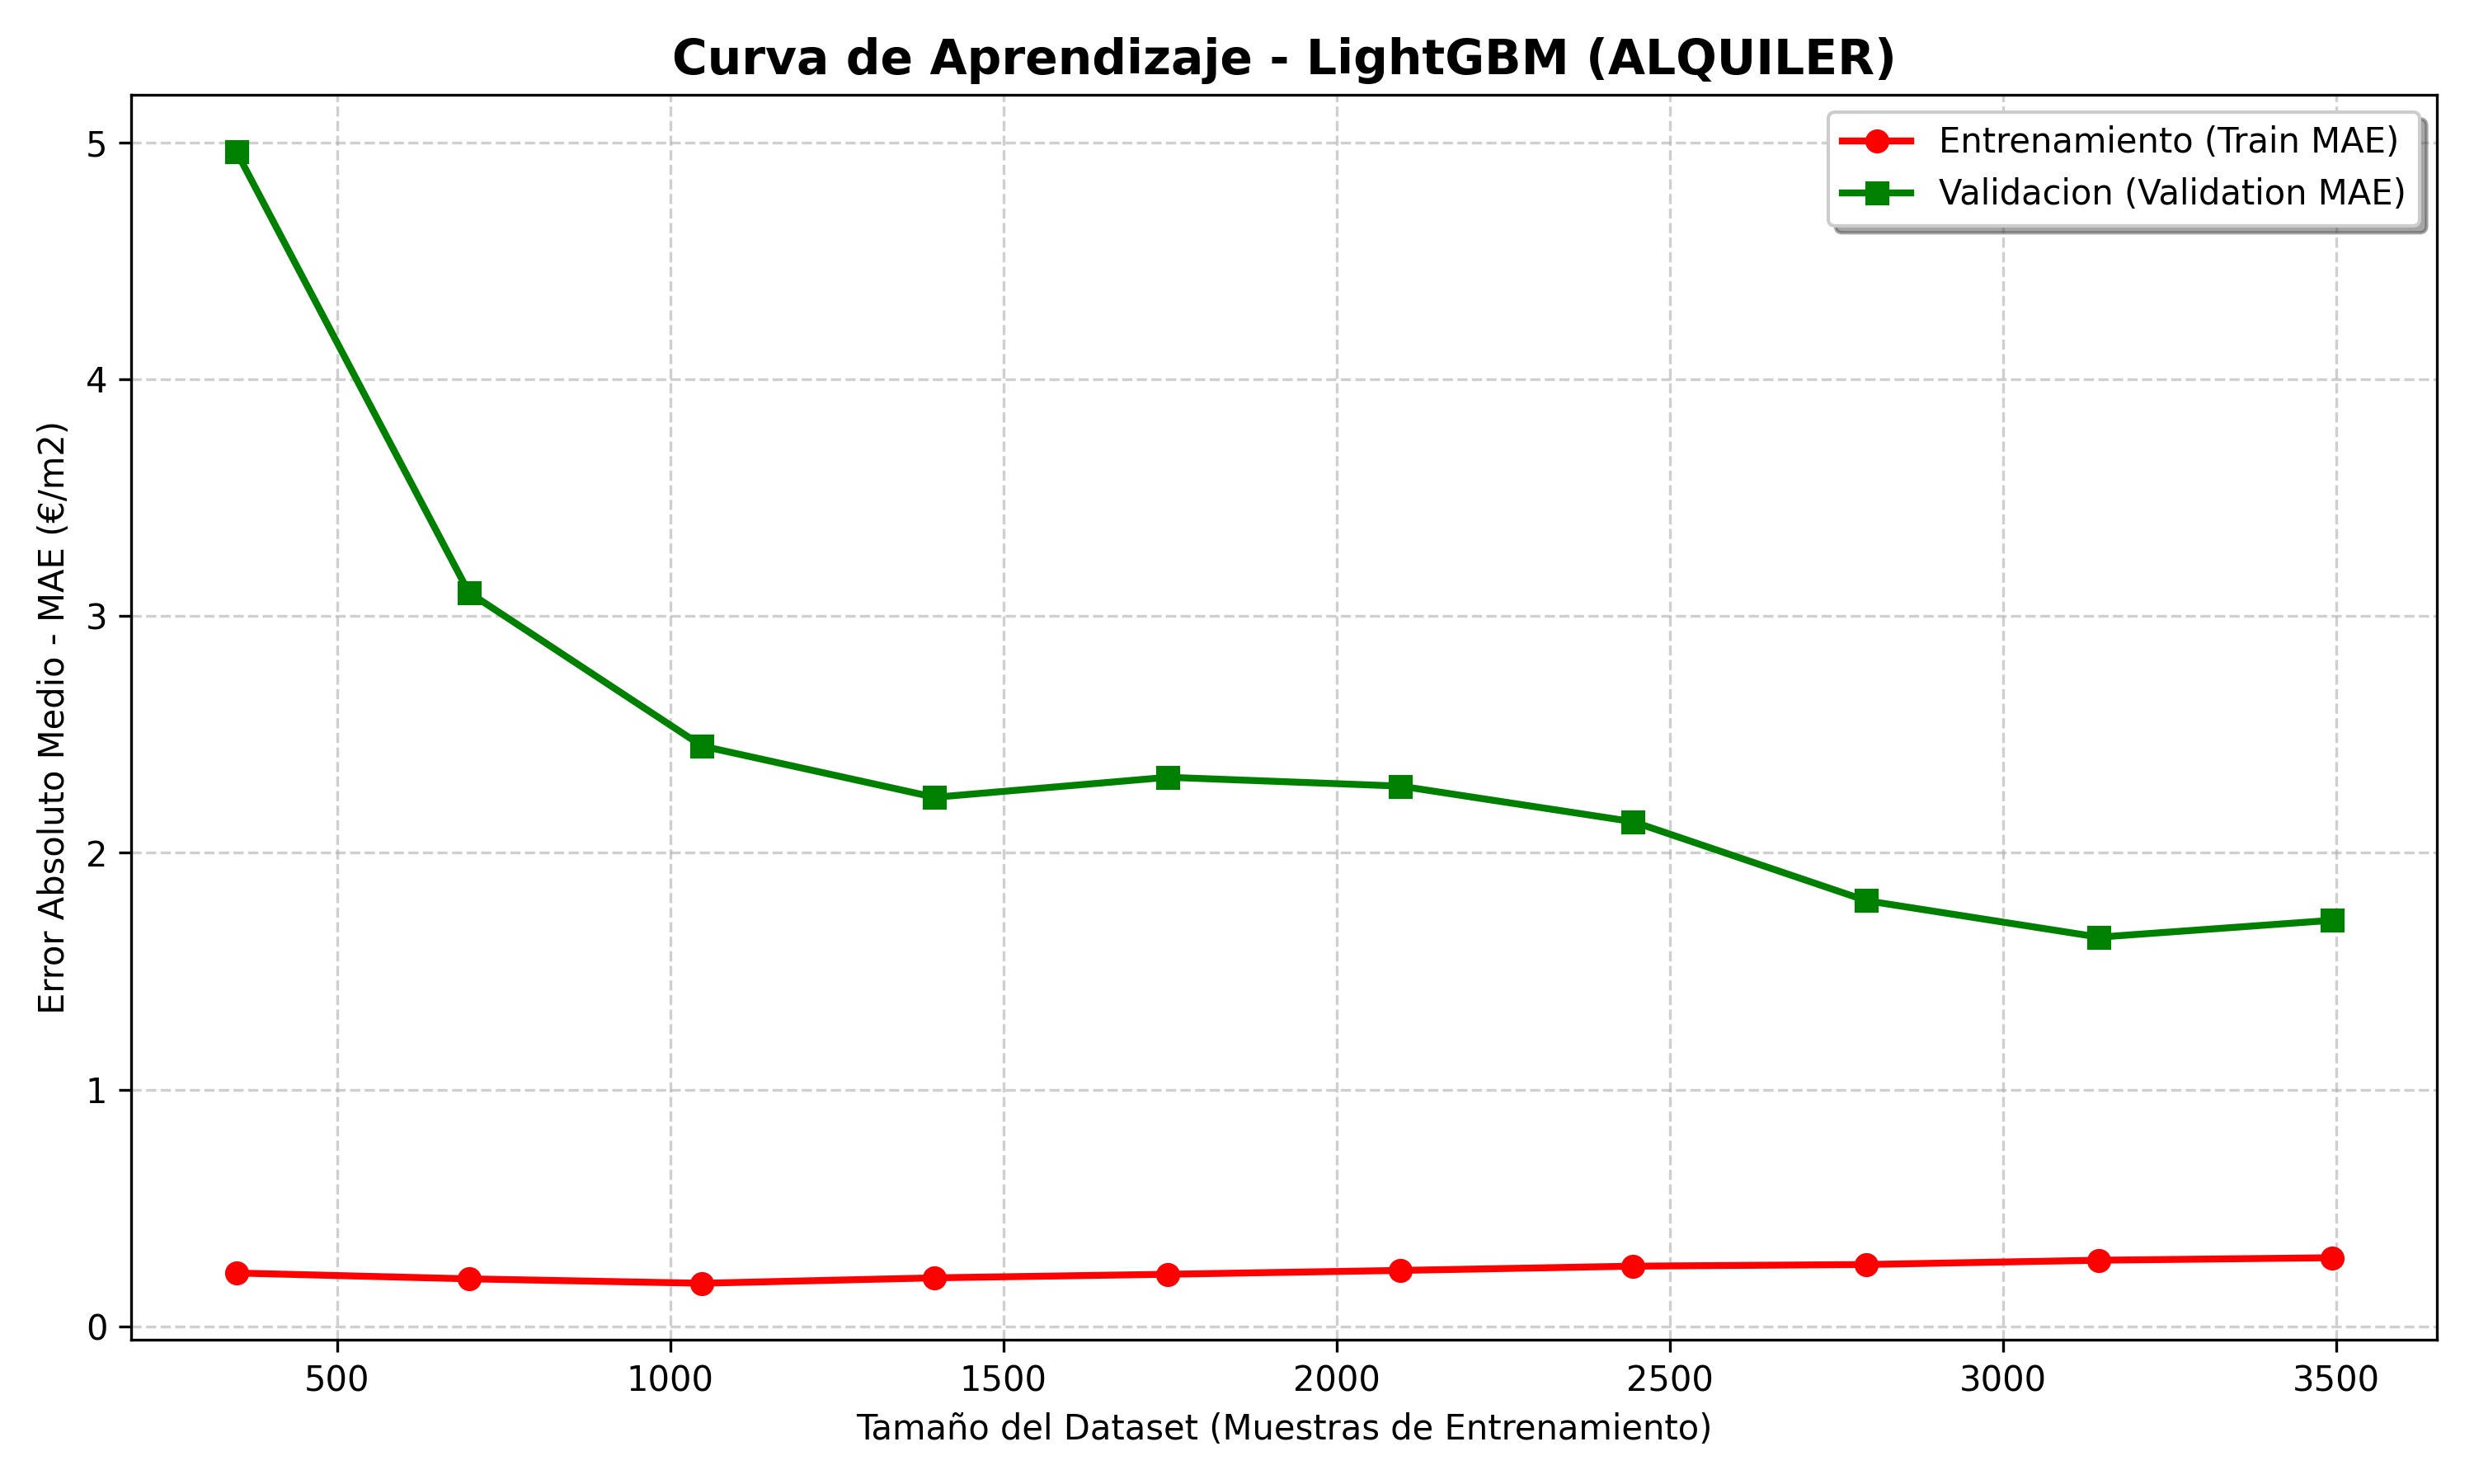
\includegraphics[width=0.40\linewidth]{img/base0_learning_curve_lightgbm_alquiler.png} \\
(c) LightGBM - Venta & (d) LightGBM - Alquiler \\
\end{tabular}
\caption{Curvas de aprendizaje de Random Forest y LightGBM para los mercados de venta y alquiler en el Escenario Inicial.}
\label{fig:learning_curves_rf_lgb}
\end{figure}

\begin{figure}[H]
\centering
\begin{tabular}{cc}
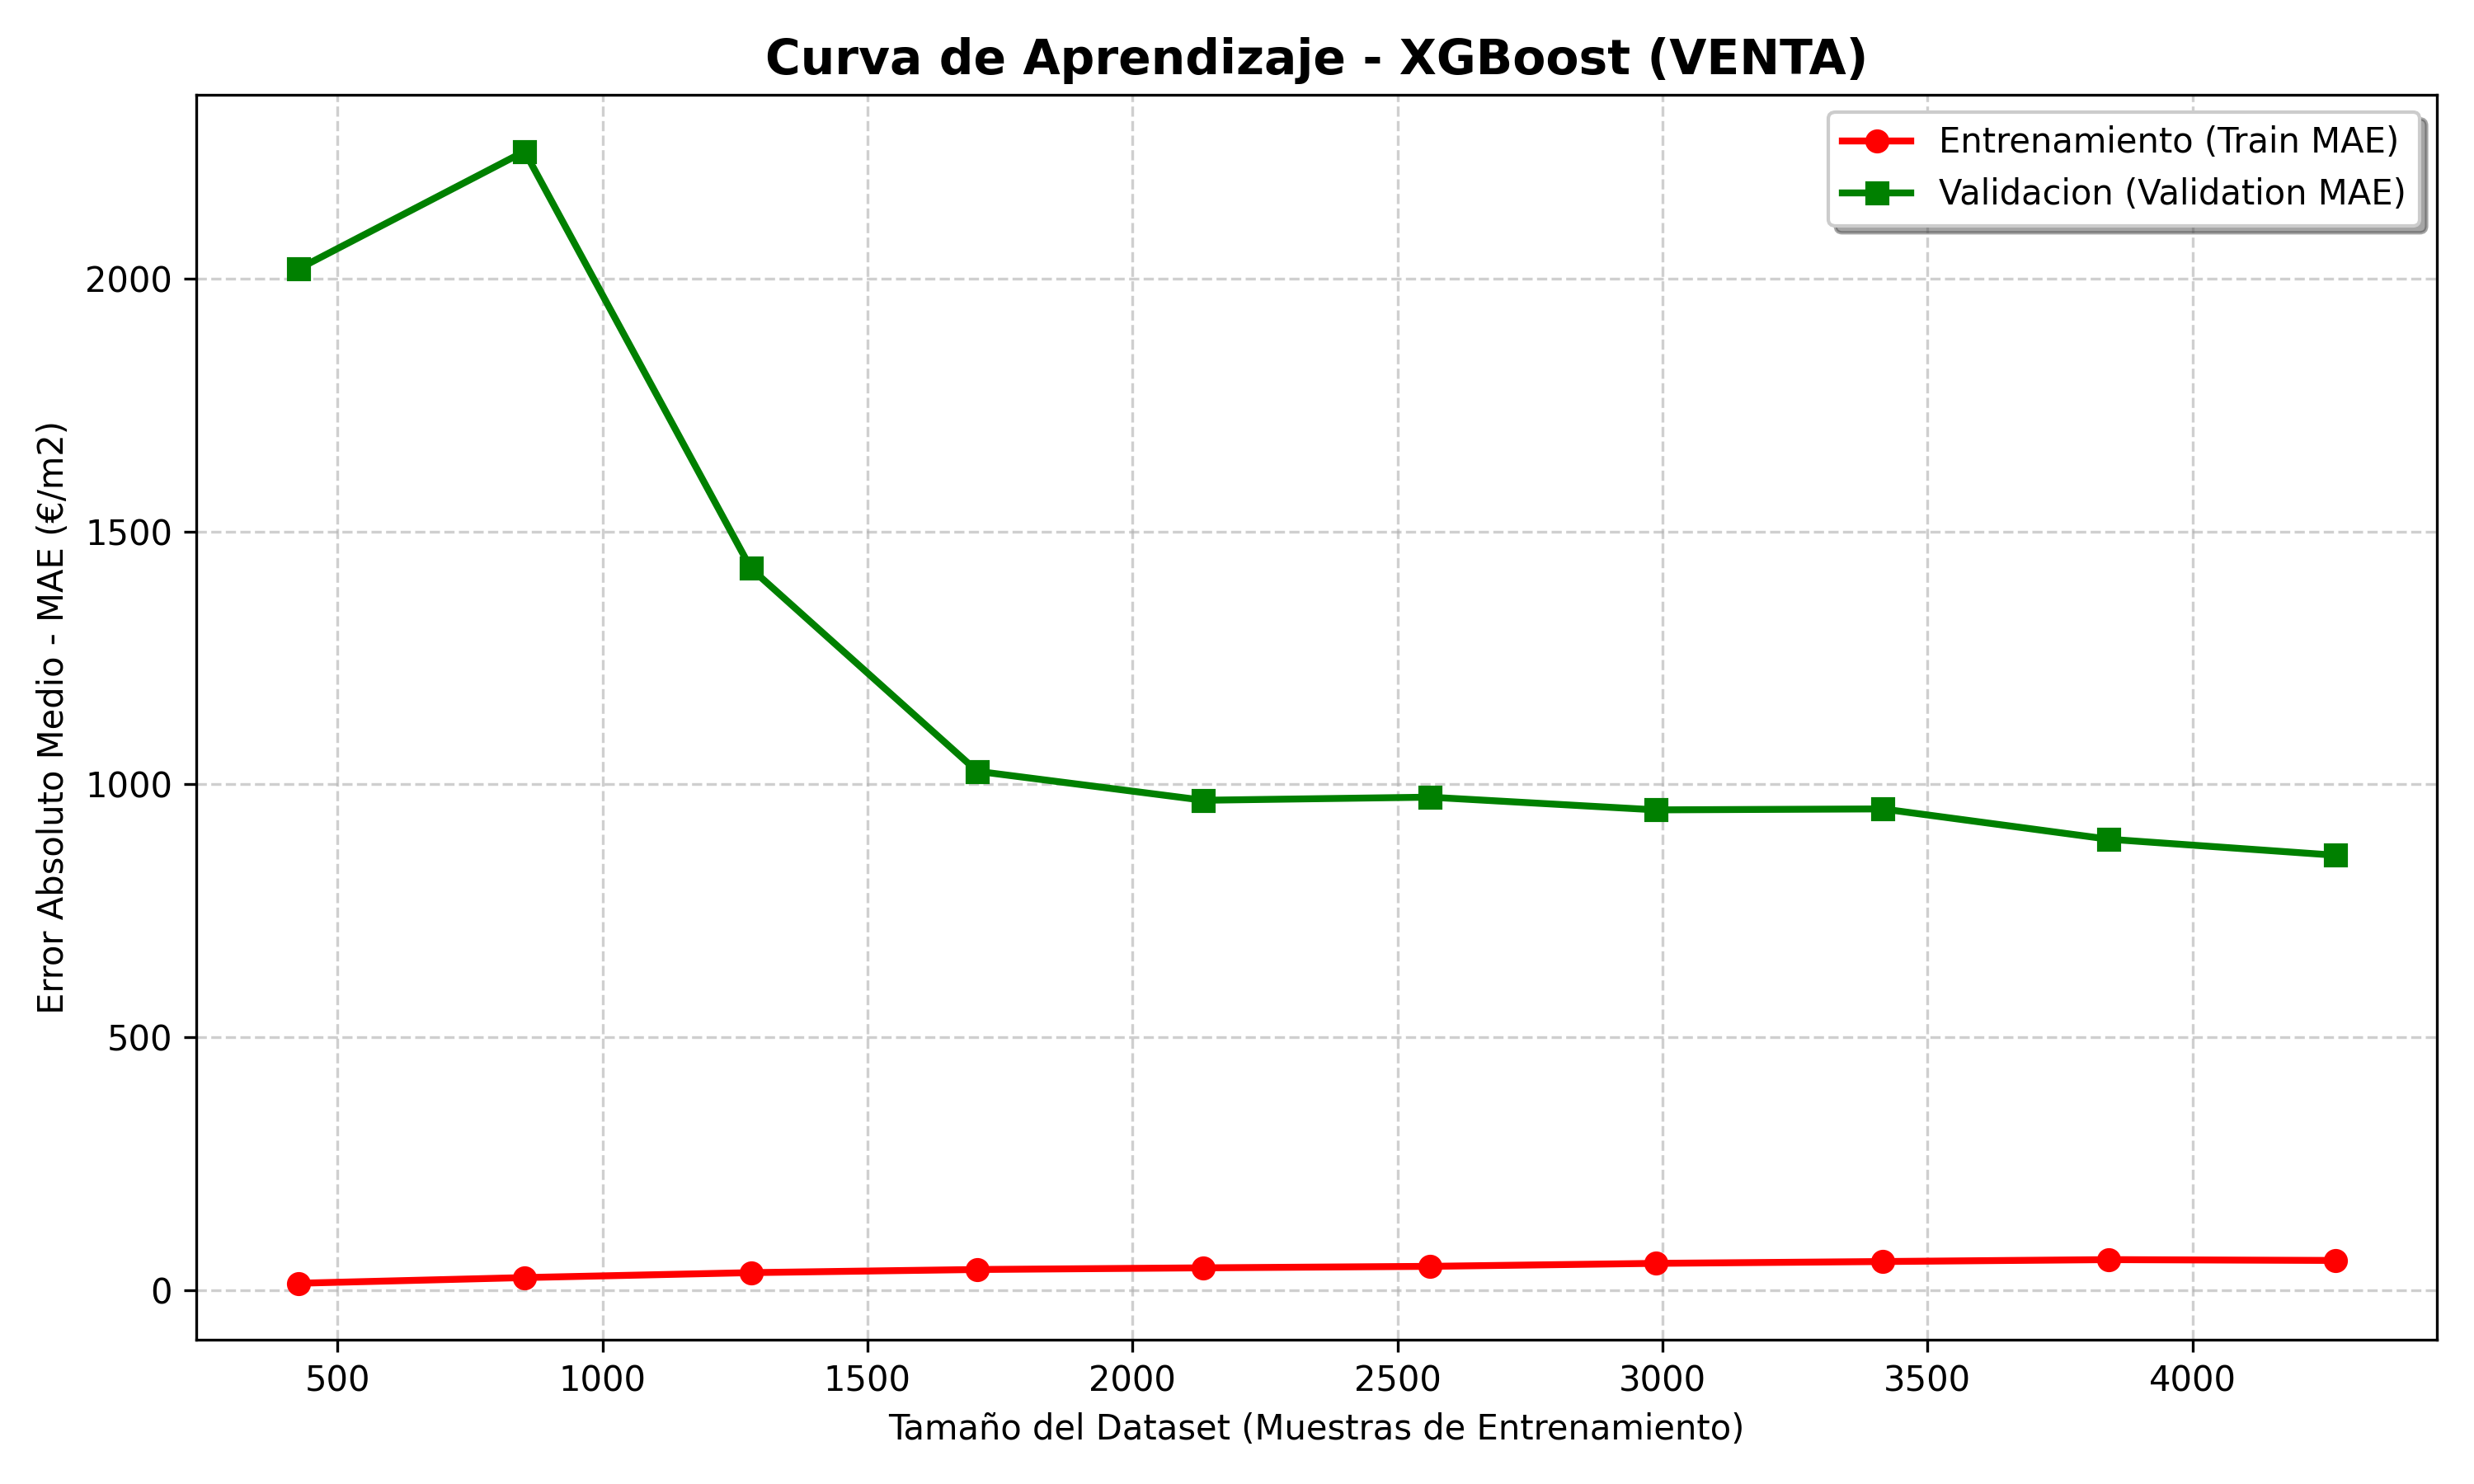
\includegraphics[width=0.40\linewidth]{img/base0_learning_curve_xgboost_venta.png} & 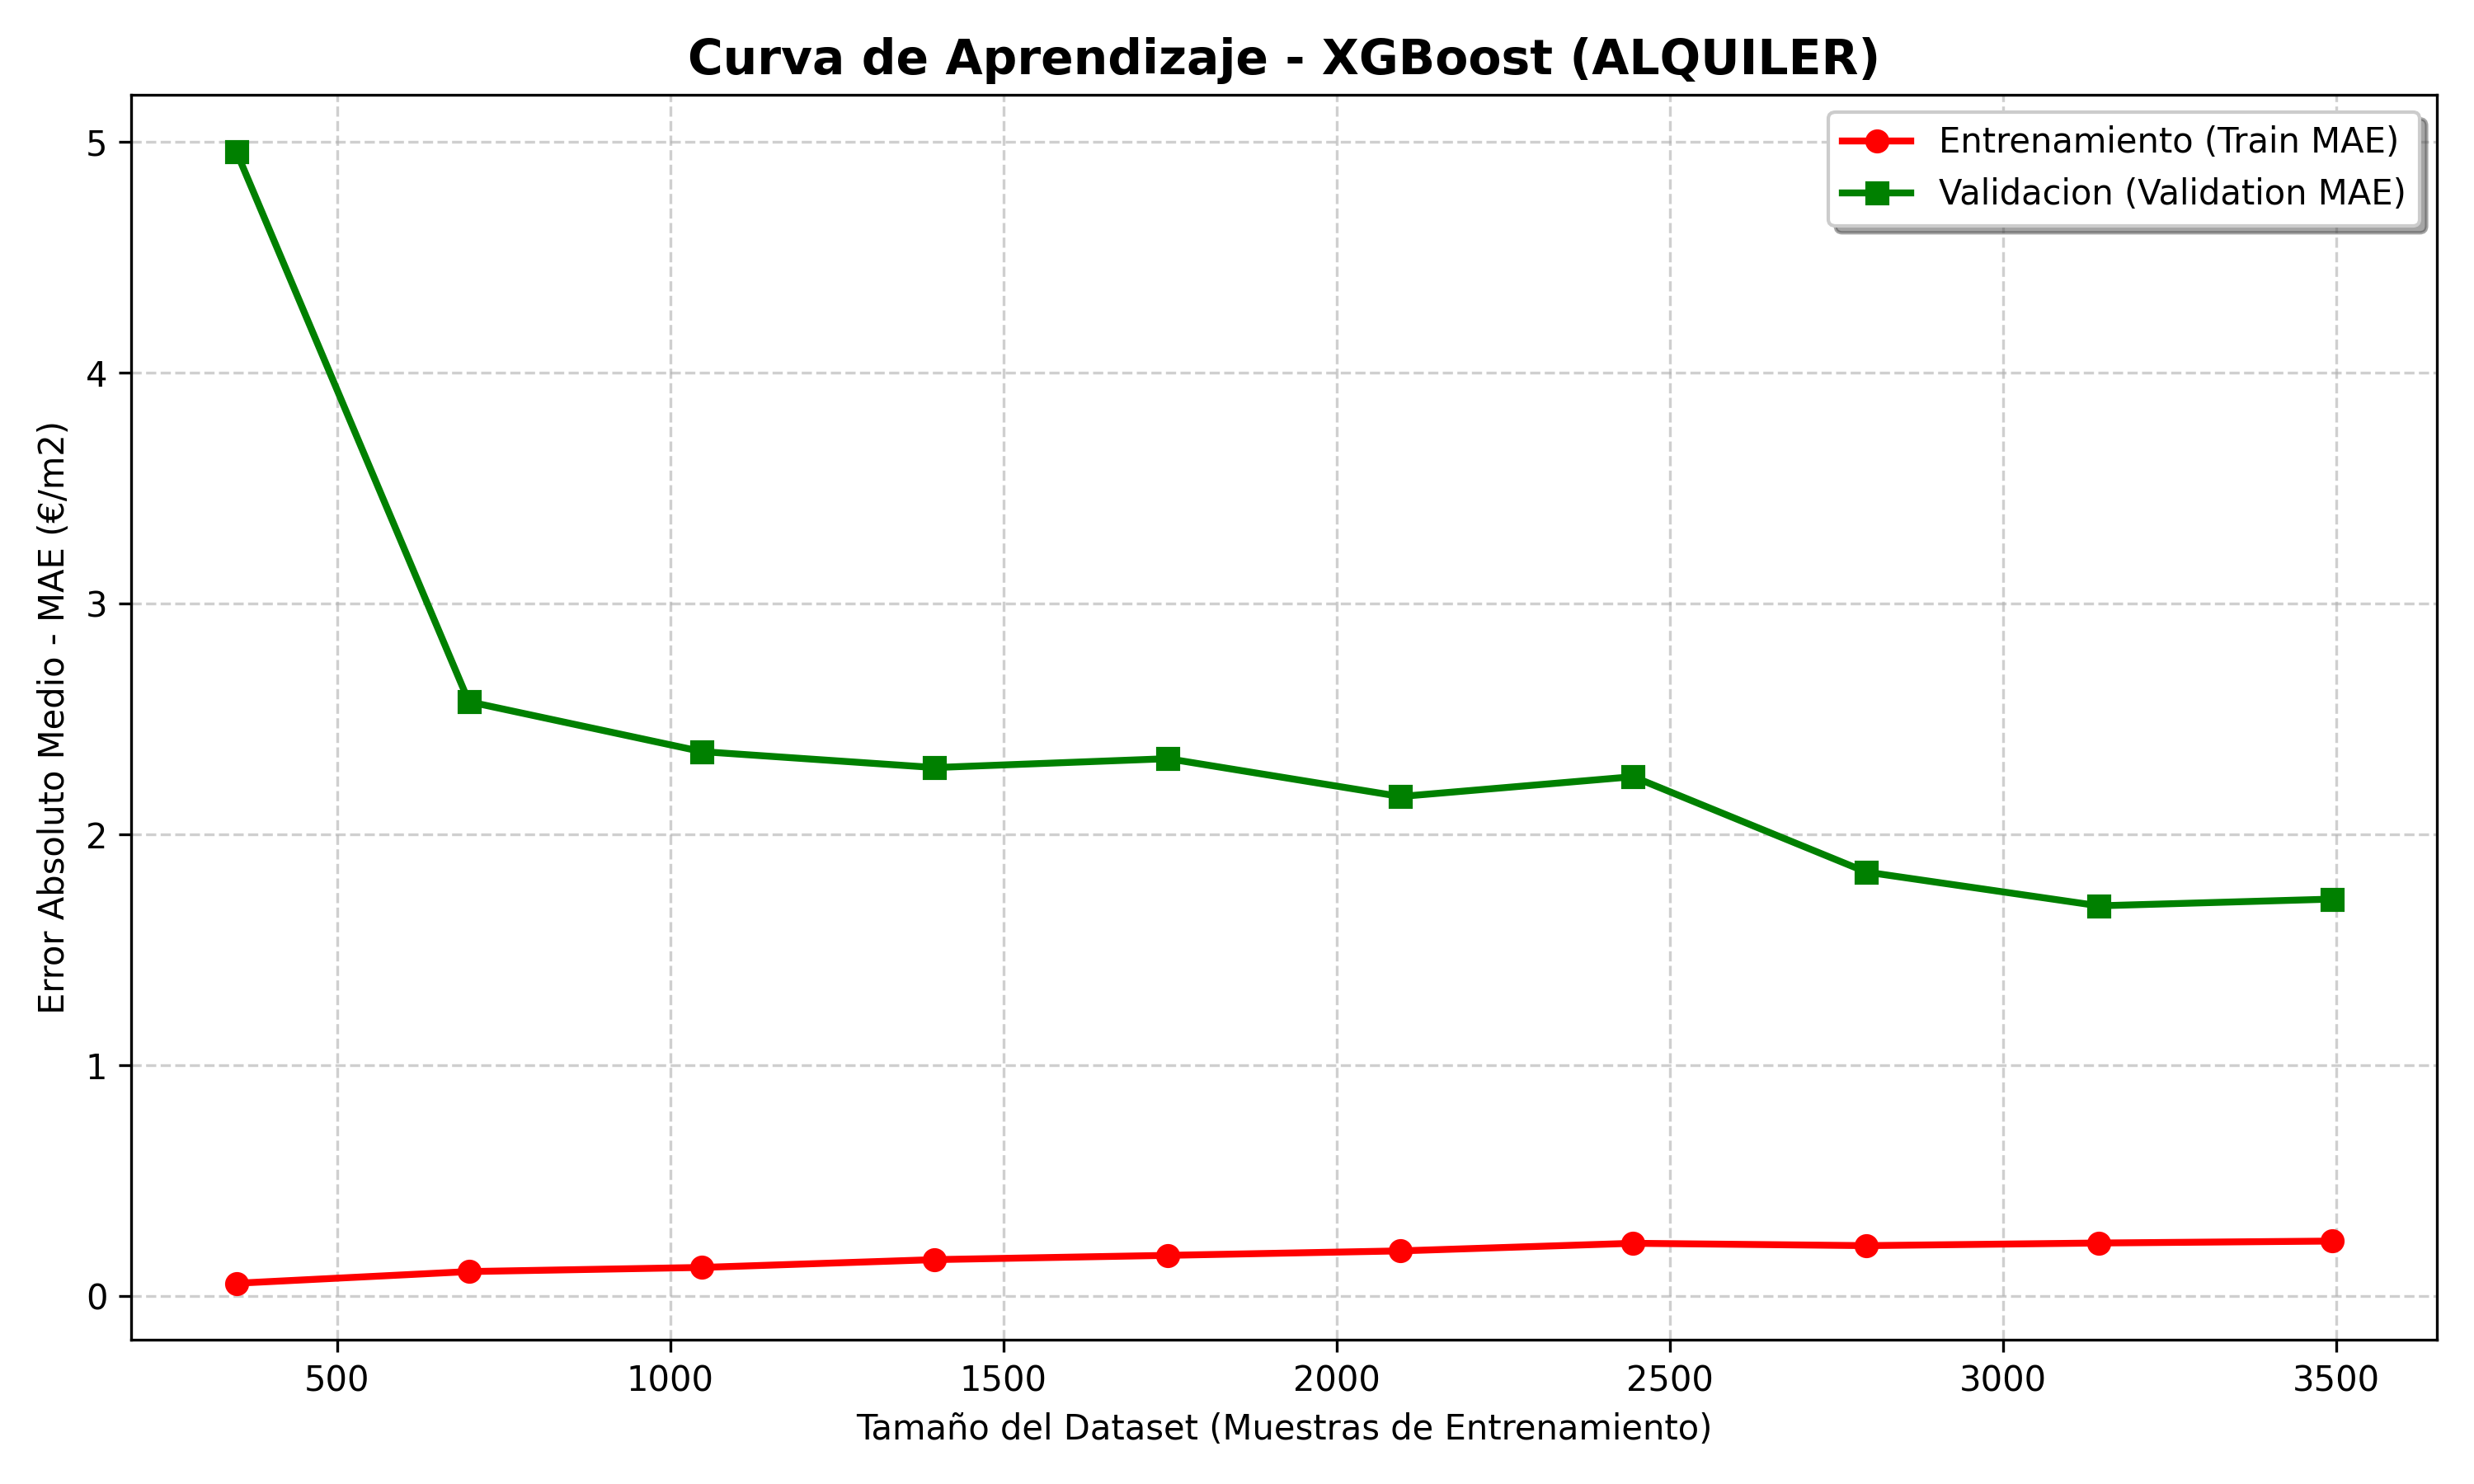
\includegraphics[width=0.40\linewidth]{img/base0_learning_curve_xgboost_alquiler.png} \\
(a) XGBoost - Venta & (b) XGBoost - Alquiler \\
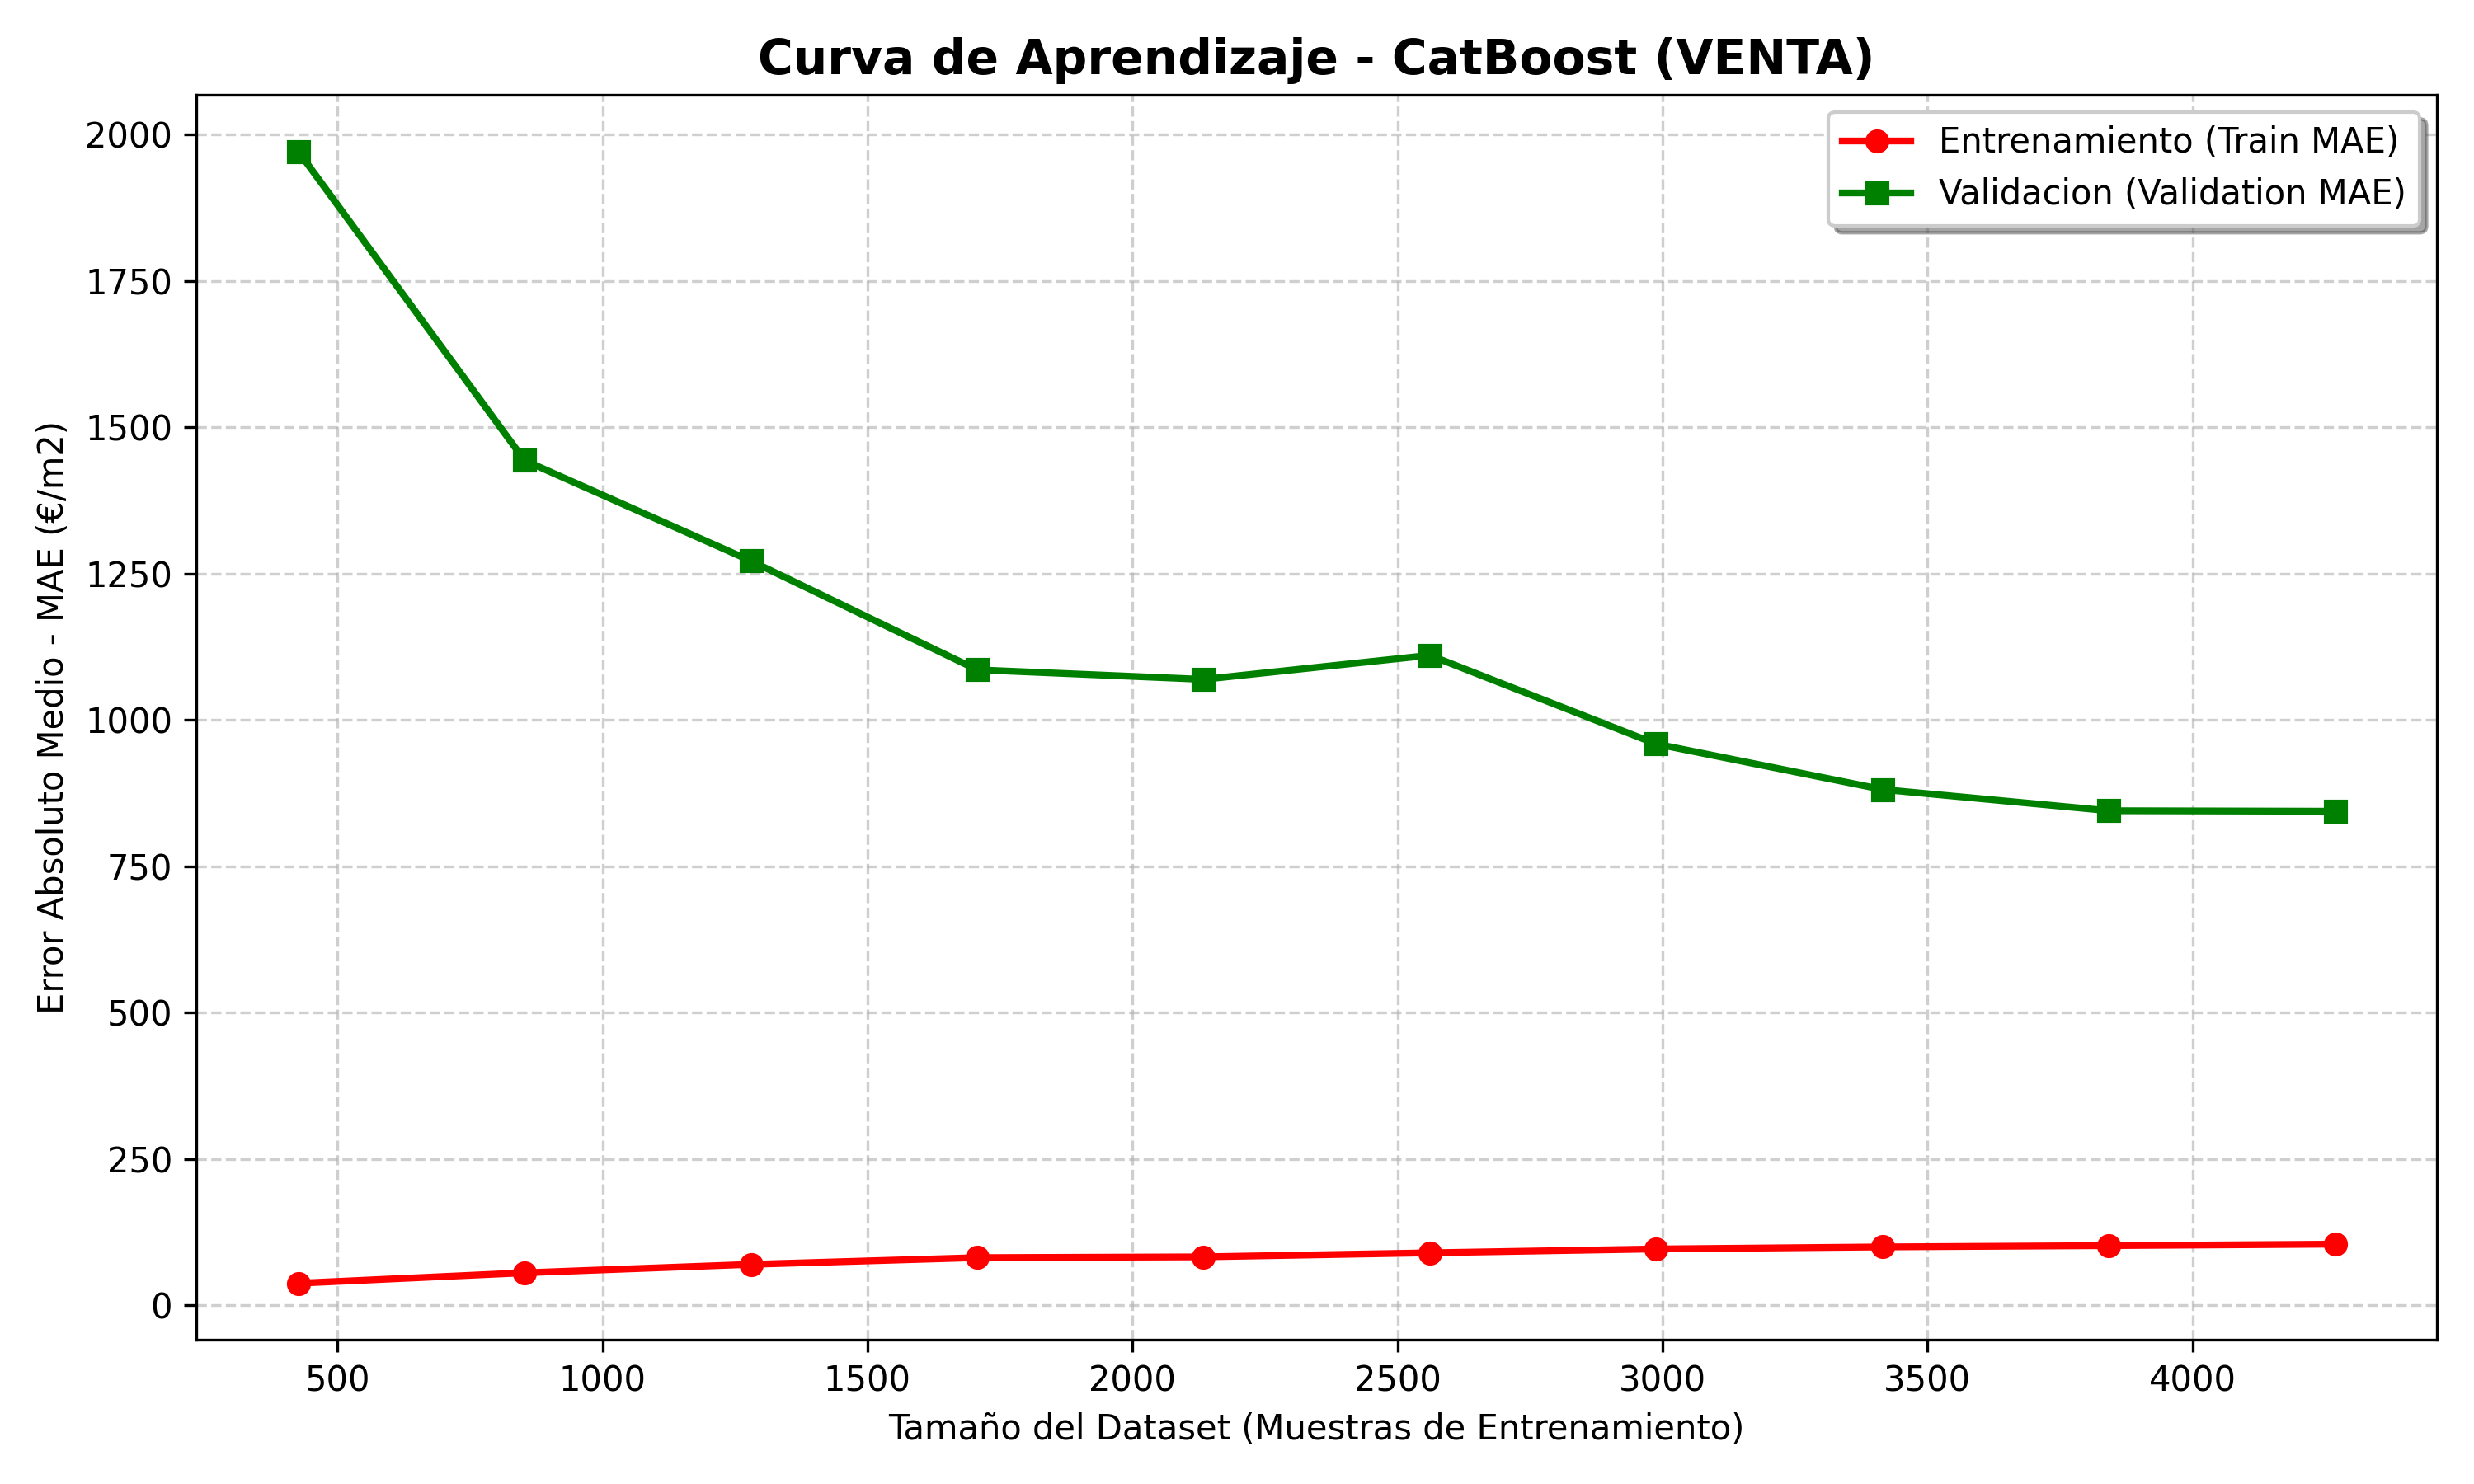
\includegraphics[width=0.40\linewidth]{img/base0_learning_curve_catboost_venta.png} & 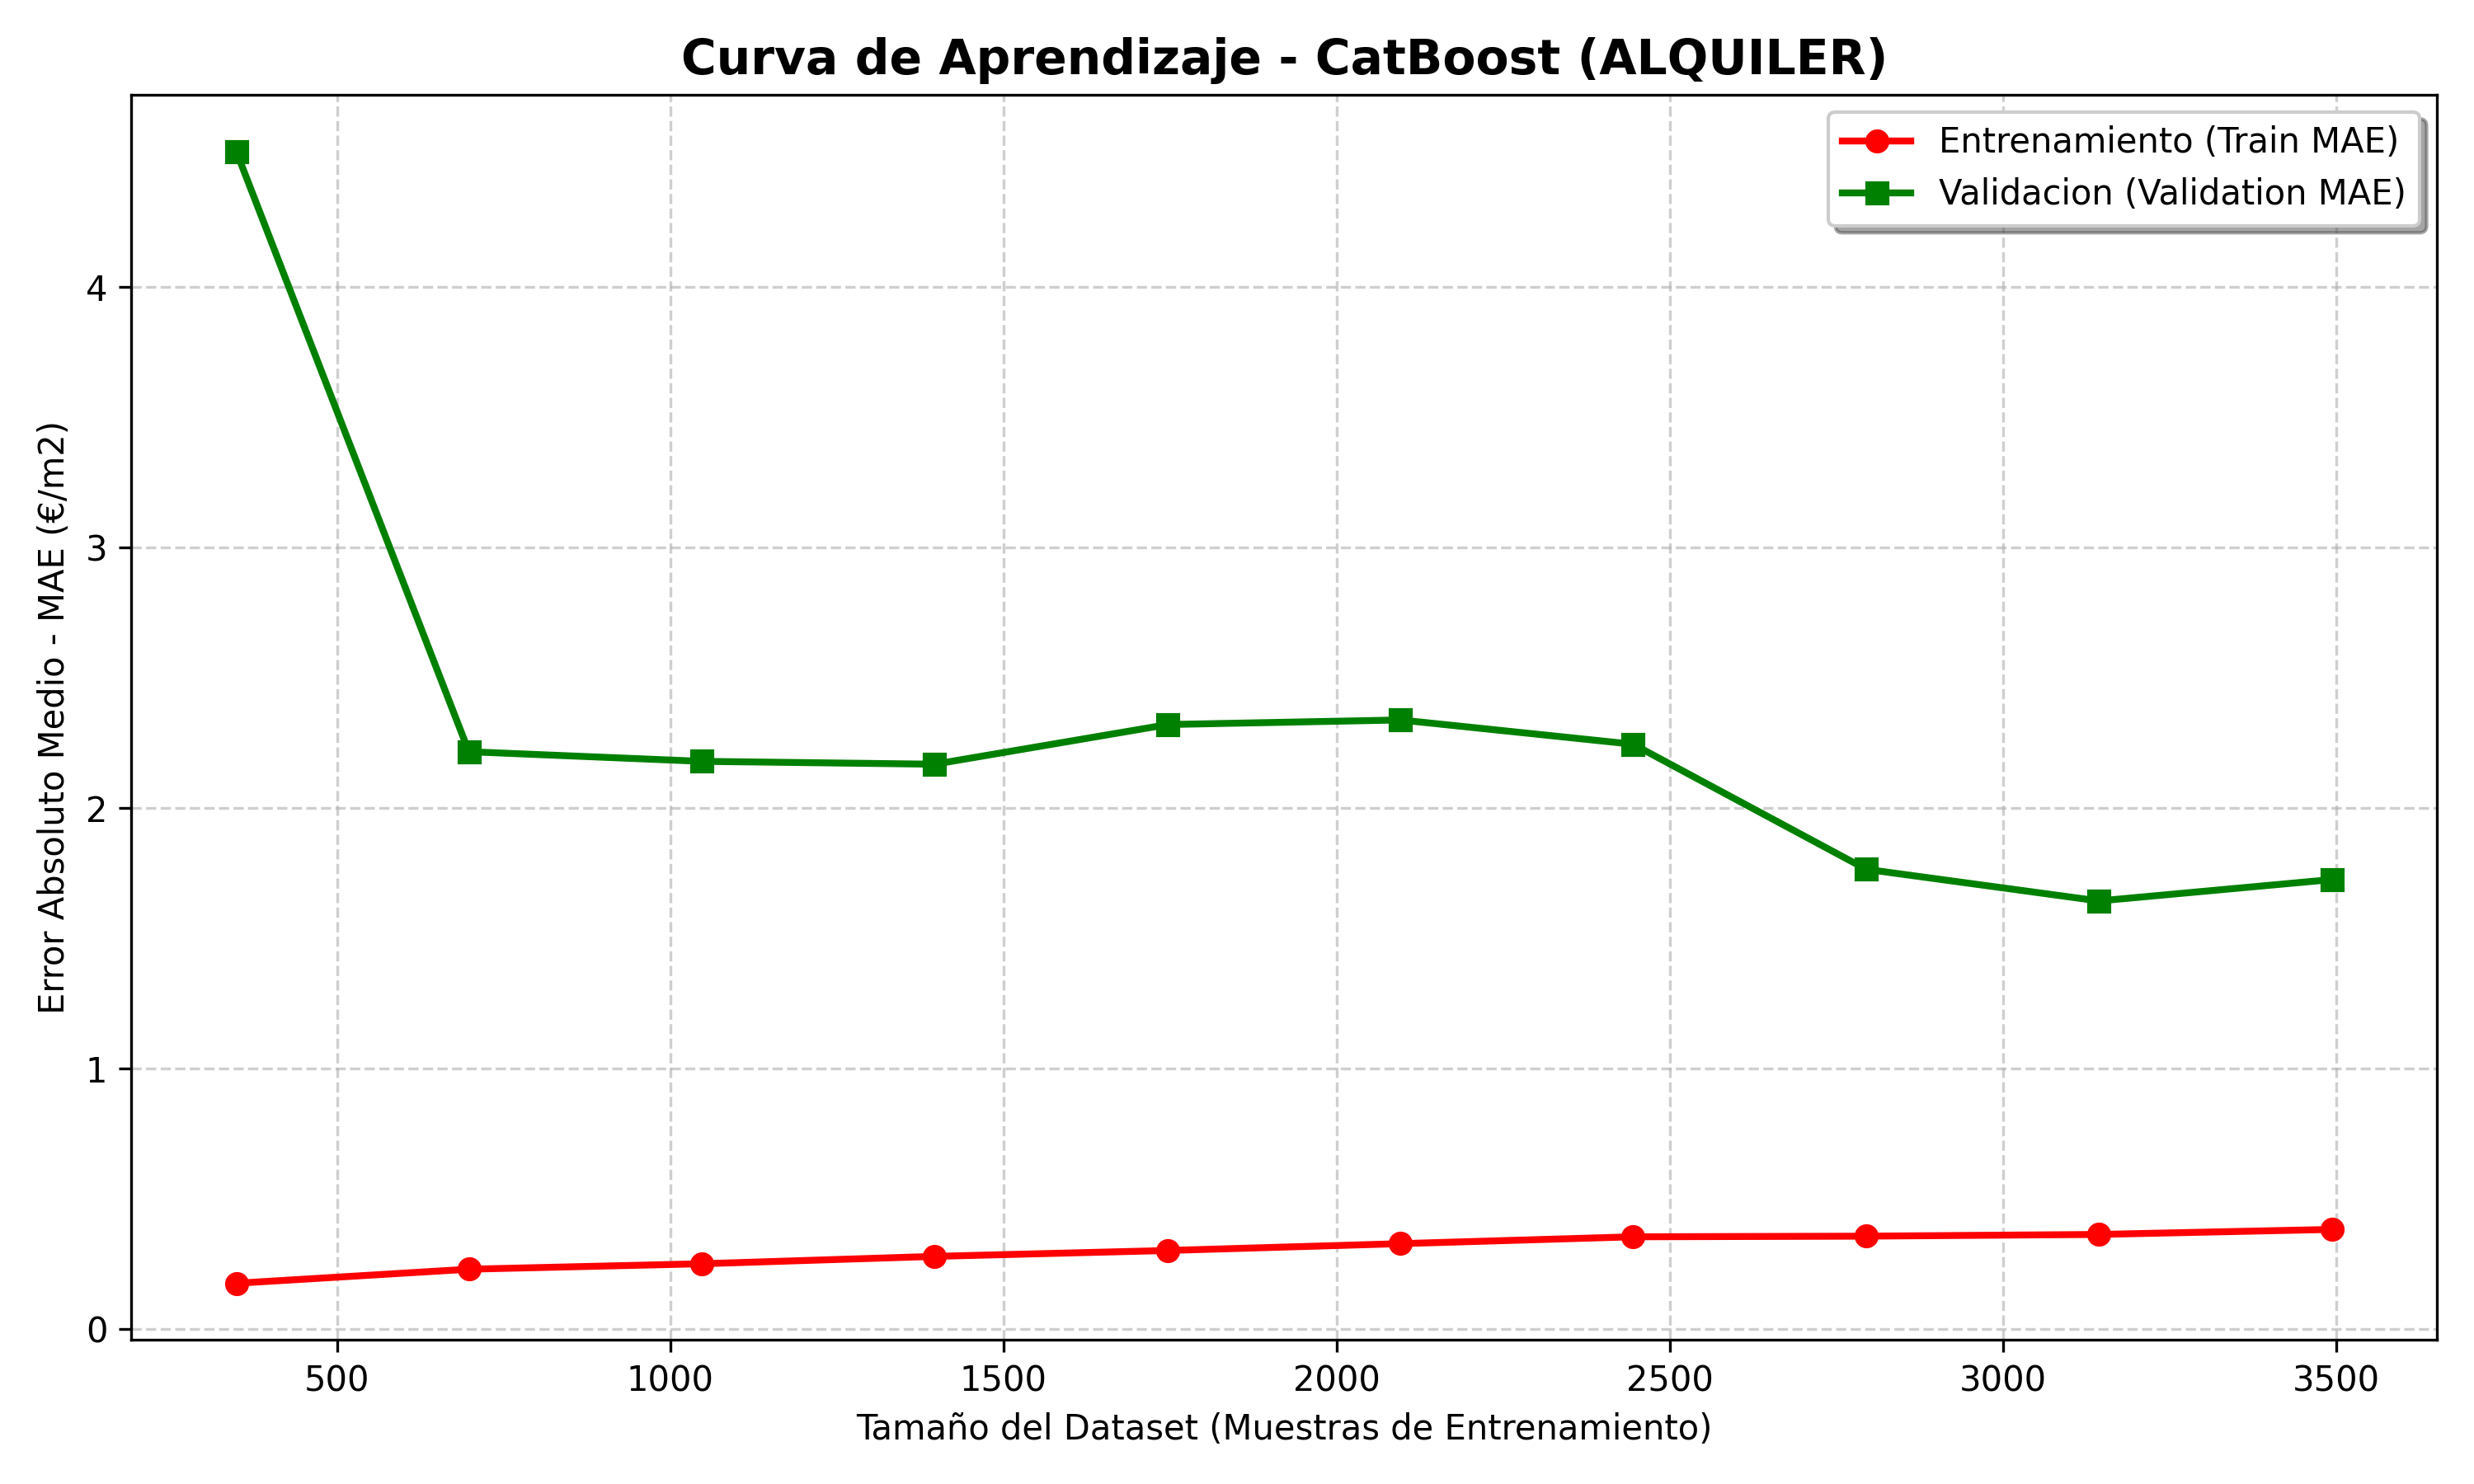
\includegraphics[width=0.40\linewidth]{img/base0_learning_curve_catboost_alquiler.png} \\
(c) CatBoost - Venta & (d) CatBoost - Alquiler \\
\end{tabular}
\caption{Curvas de aprendizaje de XGBoost y CatBoost para los mercados de venta y alquiler en el Escenario Inicial.}
\label{fig:learning_curves_xgb_cat}
\end{figure}

El objetivo principal de esta fase experimental fue medir la capacidad de generalización de cada algoritmo ante la varianza intrínseca de los datos inmobiliarios en su formato bruto. La siguiente metodología adopta un proceso secuencial de análisis de hipótesis y experimentación, evaluando de forma iterativa cómo respondían los algoritmos al incorporar estructura temporal y variables explicativas adicionales.

\subsection{Modelo Base con Retardo Temporal}
Tras verificar el rendimiento de la experimentación inicial, la investigación formuló la siguiente hipótesis metodológica: si no es posible «mirar hacia adelante» en el tiempo para realizar predicciones en producción (con el fin de evitar fugas de datos o \textit{data leakage}), la precisión del modelo debe incrementarse si introducimos información retrospectiva mediante retardos de memoria temporal.

Para validar esta hipótesis, se diseñaron y construyeron cuatro variables fundamentales de retardo e inercia histórica: \texttt{lag\_1}, \texttt{lag\_3}, \texttt{lag\_12} (para capturar la memoria de corto plazo y la estacionalidad anual) junto con una media móvil suavizada \texttt{rolling\_mean\_6} (para estabilizar el comportamiento reciente del mercado). La inyección de características de retardo (\textit{lag features}) y estadísticas de ventana móvil (\textit{rolling statistics}) representa una técnica estándar y de alta eficacia en la literatura científica para el modelado de series temporales y de consumo mediante algoritmos de Boosting. Esta aproximación se fundamenta en trabajos de referencia como el estudio de Varma et al. (2025) sobre ingeniería de características de múltiples retardos para XGBoost y CatBoost, o los estudios de benchmarking de modelos basados en árboles (Elsayed et al., 2021), en los cuales la adición de lags demostró reducir de forma sustancial el error medio absoluto (MAE) y el error cuadrático medio (RMSE) en entornos de alta volatilidad temporal. A partir de este fundamento metodológico, se procedió a evaluar el comportamiento de los modelos bajo tres enfoques de escalas geográficas progresivas.


\subsubsection{Evaluación Cruzada (Modelo de Distrito Evaluado sobre Barrios)}
Para evaluar el comportamiento de los modelos bajo un escenario de evaluación cruzada empleando memoria temporal, se replicó de forma análoga el esquema de entrenamiento a nivel de distrito y evaluación sobre barrios planteado originalmente para el modelo base en la experimentación inicial. Esto facilita aislar y contrastar de manera directa el impacto neto de las variables de memoria inercial sobre los algoritmos. Los resultados de este experimento, descritos en la Tabla~\ref{tab:phase1_crossed_venta} y la Tabla~\ref{tab:phase1_crossed_alquiler}, revelaron la influencia de las variables de retardo:

\begin{table}[H]
\centering
\caption{Matriz de rendimiento comparativa: Evaluación cruzada (distrito a barrio) con retardos temporales - Mercado de Venta (€/m\textsuperscript{2})}
\label{tab:phase1_crossed_venta}
\resizebox{\textwidth}{!}{%
\begin{tabular}{|l|c|c|c|c|c|c|c|c|c|c|c|}
\hline
\textbf{Algoritmo} & \textbf{MAE} & \textbf{RMSE} & \textbf{R\textsuperscript{2}} & \textbf{MAPE} & \textbf{Sesgo} & \textbf{MAE} & \textbf{R\textsuperscript{2}} & \textbf{MAE} & \textbf{R\textsuperscript{2}} & \textbf{T. Train} & \textbf{T. Pred} \\
 & \textbf{Global} & \textbf{Global} & \textbf{Global} & \textbf{Global (\%)} & \textbf{Global} & \textbf{Salamanca} & \textbf{Salamanca} & \textbf{C. Lineal} & \textbf{C. Lineal} & \textbf{(s)} & \textbf{(s)} \\
\hline
\textbf{Random Forest} & 152,83 & 272,82 & 0,9827 & 2,40\% & 24,96 & 302,74 & 0,8277 & \textbf{723,79} & \textbf{0,6606} & 0,712 & 0,111 \\
\textbf{CatBoost} & 258,87 & 466,94 & 0,9493 & 4,04\% & -115,83 & 275,08 & 0,8149 & 1259,27 & 0,1054 & 1,017 & 0,004 \\
\textbf{XGBoost} & \textbf{143,81} & \textbf{261,94} & \textbf{0,9840} & \textbf{2,37\%} & \textbf{-10,64} & \textbf{124,64} & \textbf{0,9610} & 736,37 & 0,6523 & 0,278 & 0,004 \\
\textbf{LightGBM} & 215,56 & 398,20 & 0,9631 & 3,22\% & -11,56 & 314,01 & 0,7927 & 1152,29 & 0,3051 & \textbf{0,192} & \textbf{0,003} \\
\hline
\end{tabular}%
}
\end{table}

\begin{table}[H]
\centering
\caption{Matriz de rendimiento comparativa: Evaluación cruzada (distrito a barrio) con retardos temporales - Mercado de Alquiler (€/m\textsuperscript{2})}
\label{tab:phase1_crossed_alquiler}
\resizebox{\textwidth}{!}{%
\begin{tabular}{|l|c|c|c|c|c|c|c|c|c|c|c|}
\hline
\textbf{Algoritmo} & \textbf{MAE} & \textbf{RMSE} & \textbf{R\textsuperscript{2}} & \textbf{MAPE} & \textbf{Sesgo} & \textbf{MAE} & \textbf{R\textsuperscript{2}} & \textbf{MAE} & \textbf{R\textsuperscript{2}} & \textbf{T. Train} & \textbf{T. Pred} \\
 & \textbf{Global} & \textbf{Global} & \textbf{Global} & \textbf{Global (\%)} & \textbf{Global} & \textbf{Salamanca} & \textbf{Salamanca} & \textbf{C. Lineal} & \textbf{C. Lineal} & \textbf{(s)} & \textbf{(s)} \\
\hline
\textbf{Random Forest} & \textbf{0,599} & 0,868 & 0,9495 & \textbf{2,72\%} & -0,075 & 0,701 & 0,2796 & 1,721 & 0,5784 & 0,632 & 0,072 \\
\textbf{CatBoost} & 0,873 & 1,317 & 0,8838 & 3,77\% & -0,361 & 1,828 & -2,0330 & 2,875 & 0,0020 & 1,034 & 0,003 \\
\textbf{XGBoost} & 0,600 & \textbf{0,865} & \textbf{0,9499} & 2,74\% & \textbf{-0,070} & \textbf{0,690} & \textbf{0,3266} & \textbf{1,702} & \textbf{0,5970} & 0,199 & 0,003 \\
\textbf{LightGBM} & 0,724 & 1,112 & 0,9172 & 3,17\% & -0,180 & 1,197 & -0,7182 & 2,468 & 0,2310 & \textbf{0,091} & \textbf{0,002} \\
\hline
\end{tabular}%
}
\end{table}

El análisis comparativo detallado respecto al Escenario Inicial demuestra de forma contundente la efectividad de la inyección de inercia histórica. Todos los algoritmos experimentaron reducciones de error netas excepcionales: el MAE global en venta de XGBoost descendió de los 859,63 €/m\textsuperscript{2} iniciales a tan solo \textbf{143,81 €/m\textsuperscript{2}} (con un coeficiente de determinación R\textsuperscript{2} de 0,9840), mientras que en alquiler el error se redujo a los \textbf{0,60 €/m\textsuperscript{2}} (R\textsuperscript{2} de 0,9499). En la misma línea, Random Forest y CatBoost disminuyeron significativamente sus márgenes de error globales. En términos de latencia computacional, LightGBM continuó como la alternativa más eficiente, con únicamente $0,192$ segundos para completar su entrenamiento en el mercado de venta y $0,091$ segundos en el de alquiler. No obstante, a pesar de esta mejora drástica generalizada provocada por las características de retardo, el desajuste de escalas geográficas (entrenar con distritos homogeneizados y validar con micro-barrios heterogéneos) impidió alcanzar una precisión óptima en zonas de alta dispersión inmobiliaria. Por ejemplo, en el distrito de Salamanca, el MAE en venta fue de 124,64 €/m\textsuperscript{2} para XGBoost y de 302,74 €/m\textsuperscript{2} para Random Forest, lo que pone de relieve la necesidad de alinear las escalas territoriales.

Adicionalmente, se generaron las curvas de aprendizaje para monitorizar el entrenamiento de los algoritmos en esta primera fase con lags temporales. Las Figuras~\ref{fig:learning_curves_phase1_rf_lgb} y~\ref{fig:learning_curves_phase1_xgb_cat} exponen la evolución del error absoluto medio a lo largo del proceso. Como se observa en los gráficos, la incorporación de memoria temporal facilita una convergencia mucho más estable y veloz en todos los modelos predictivos, con una reducción del gradiente constante hasta estabilizarse en los umbrales óptimos de error; LightGBM y XGBoost se mantienen libres de sobreajuste crítico.

\begin{figure}[H]
\centering
\begin{tabular}{cc}
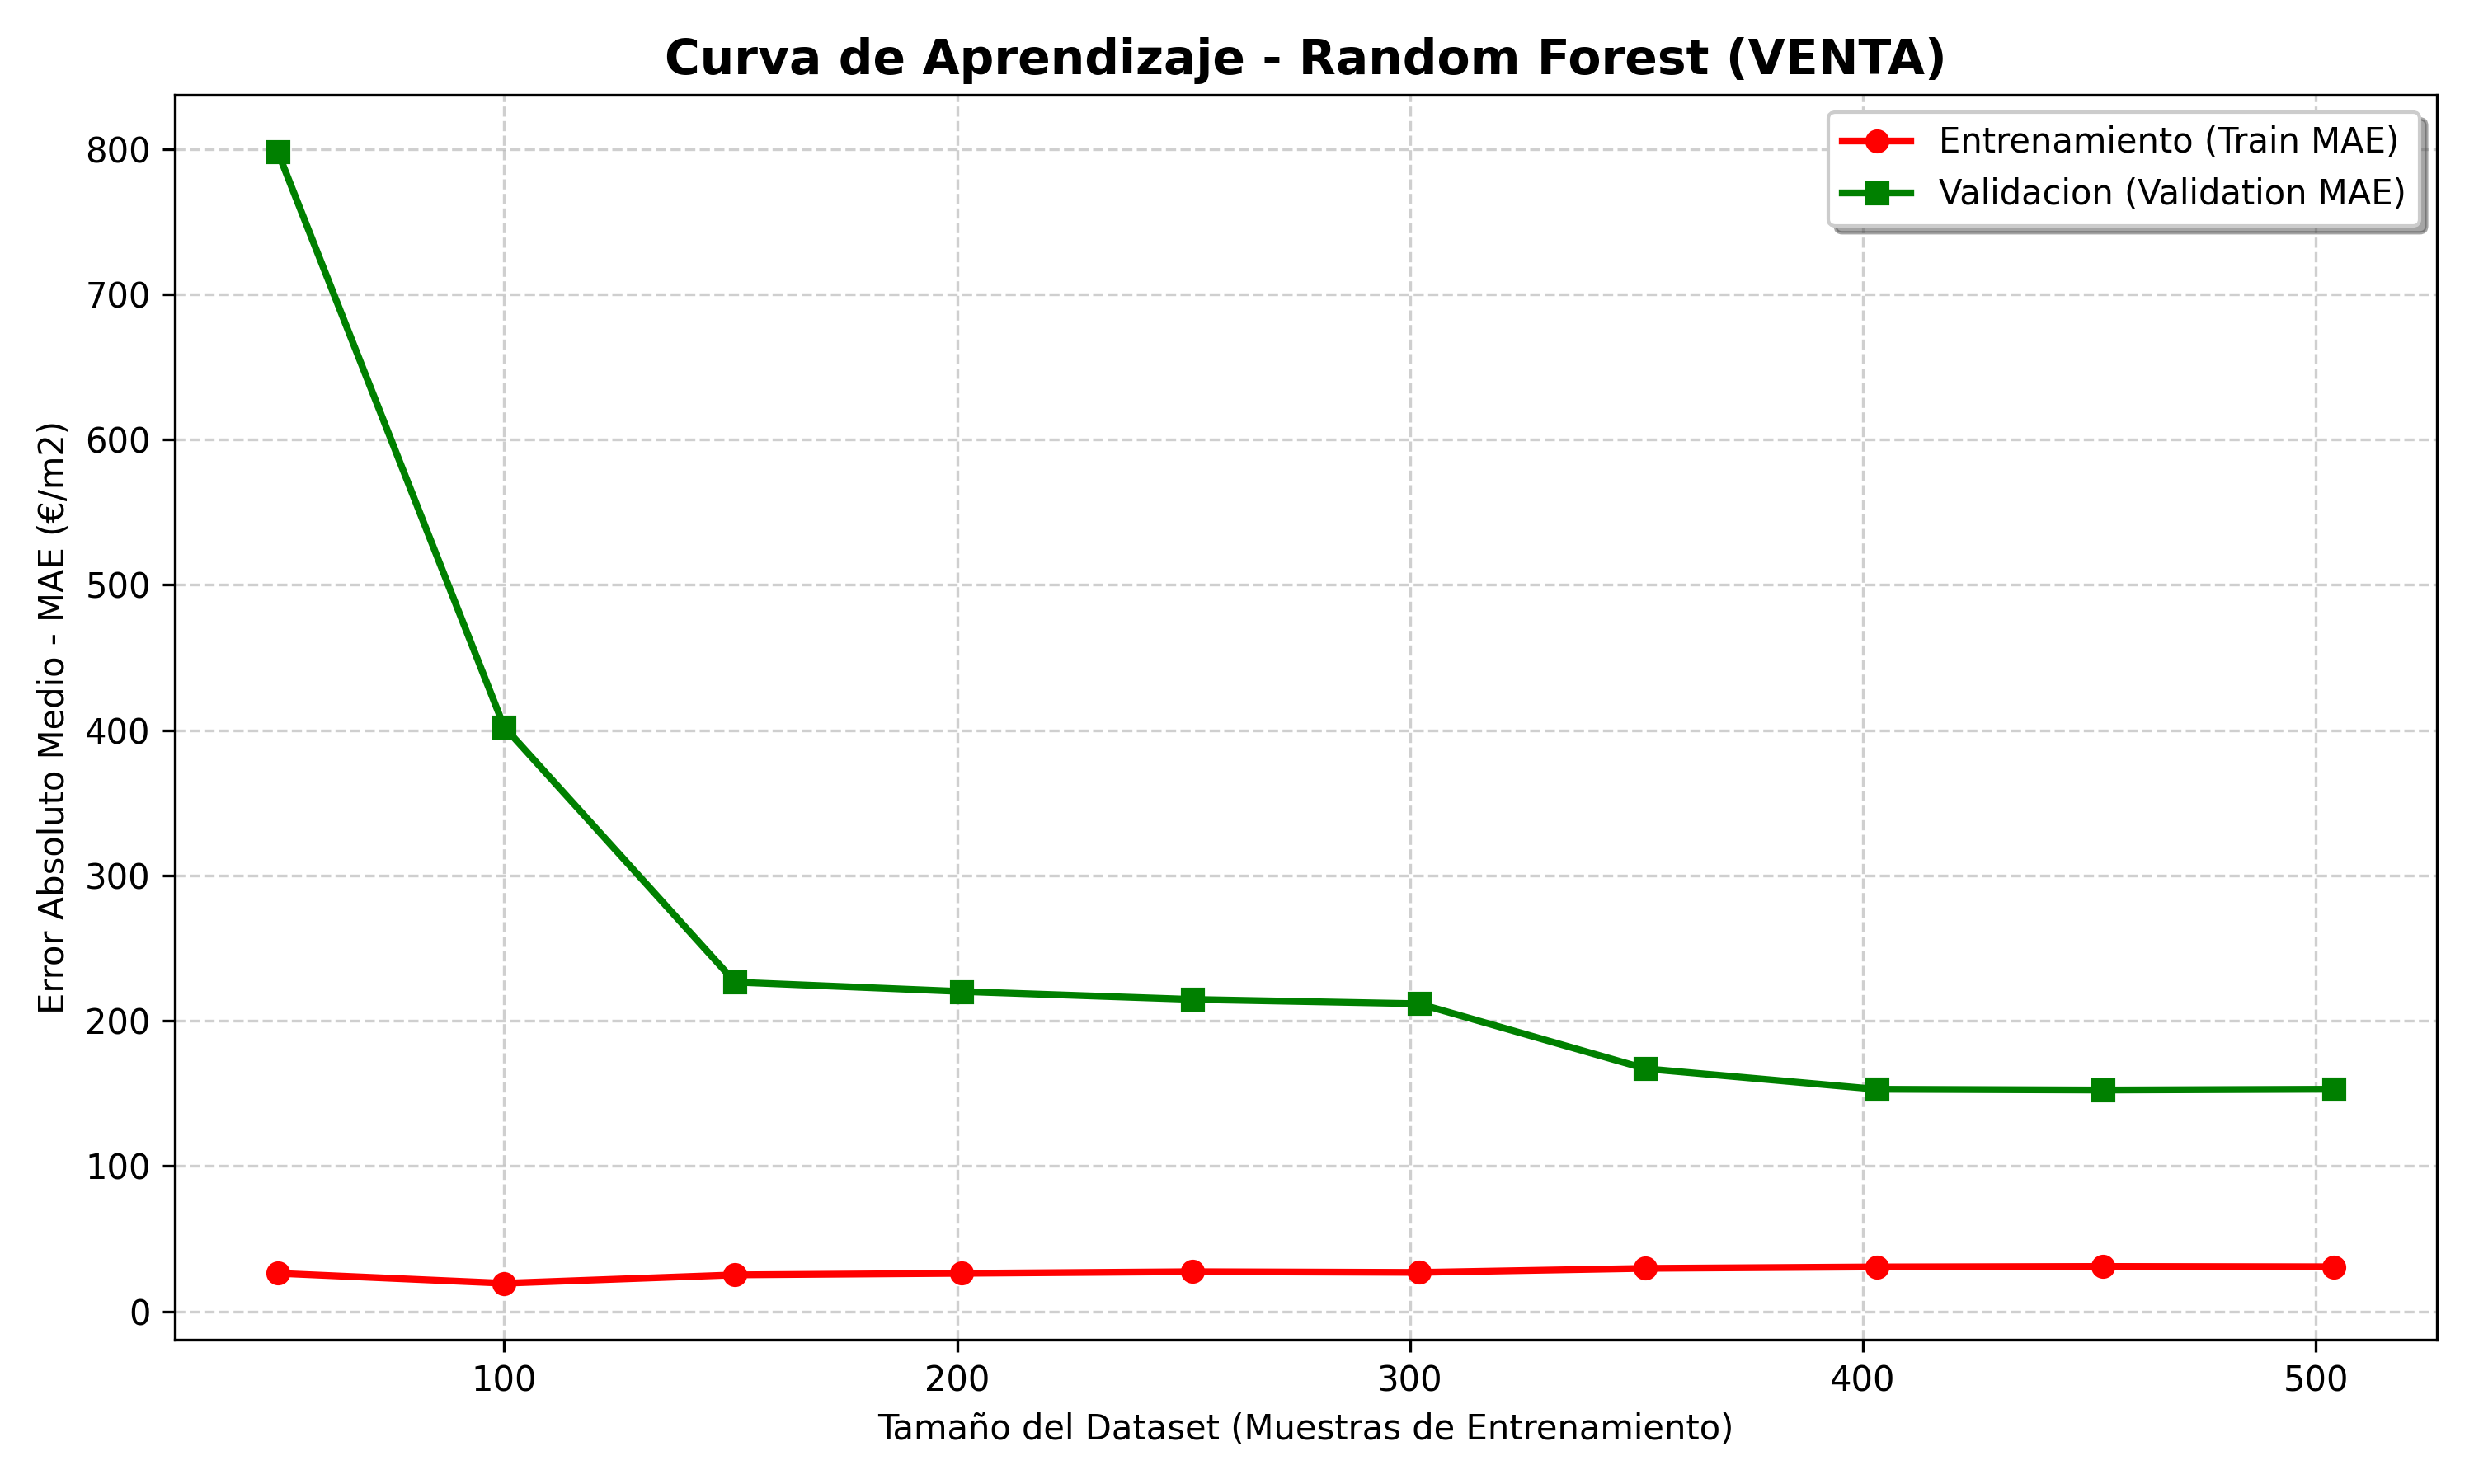
\includegraphics[width=0.40\linewidth]{img/phase1_learning_curve_random_forest_venta.png} & 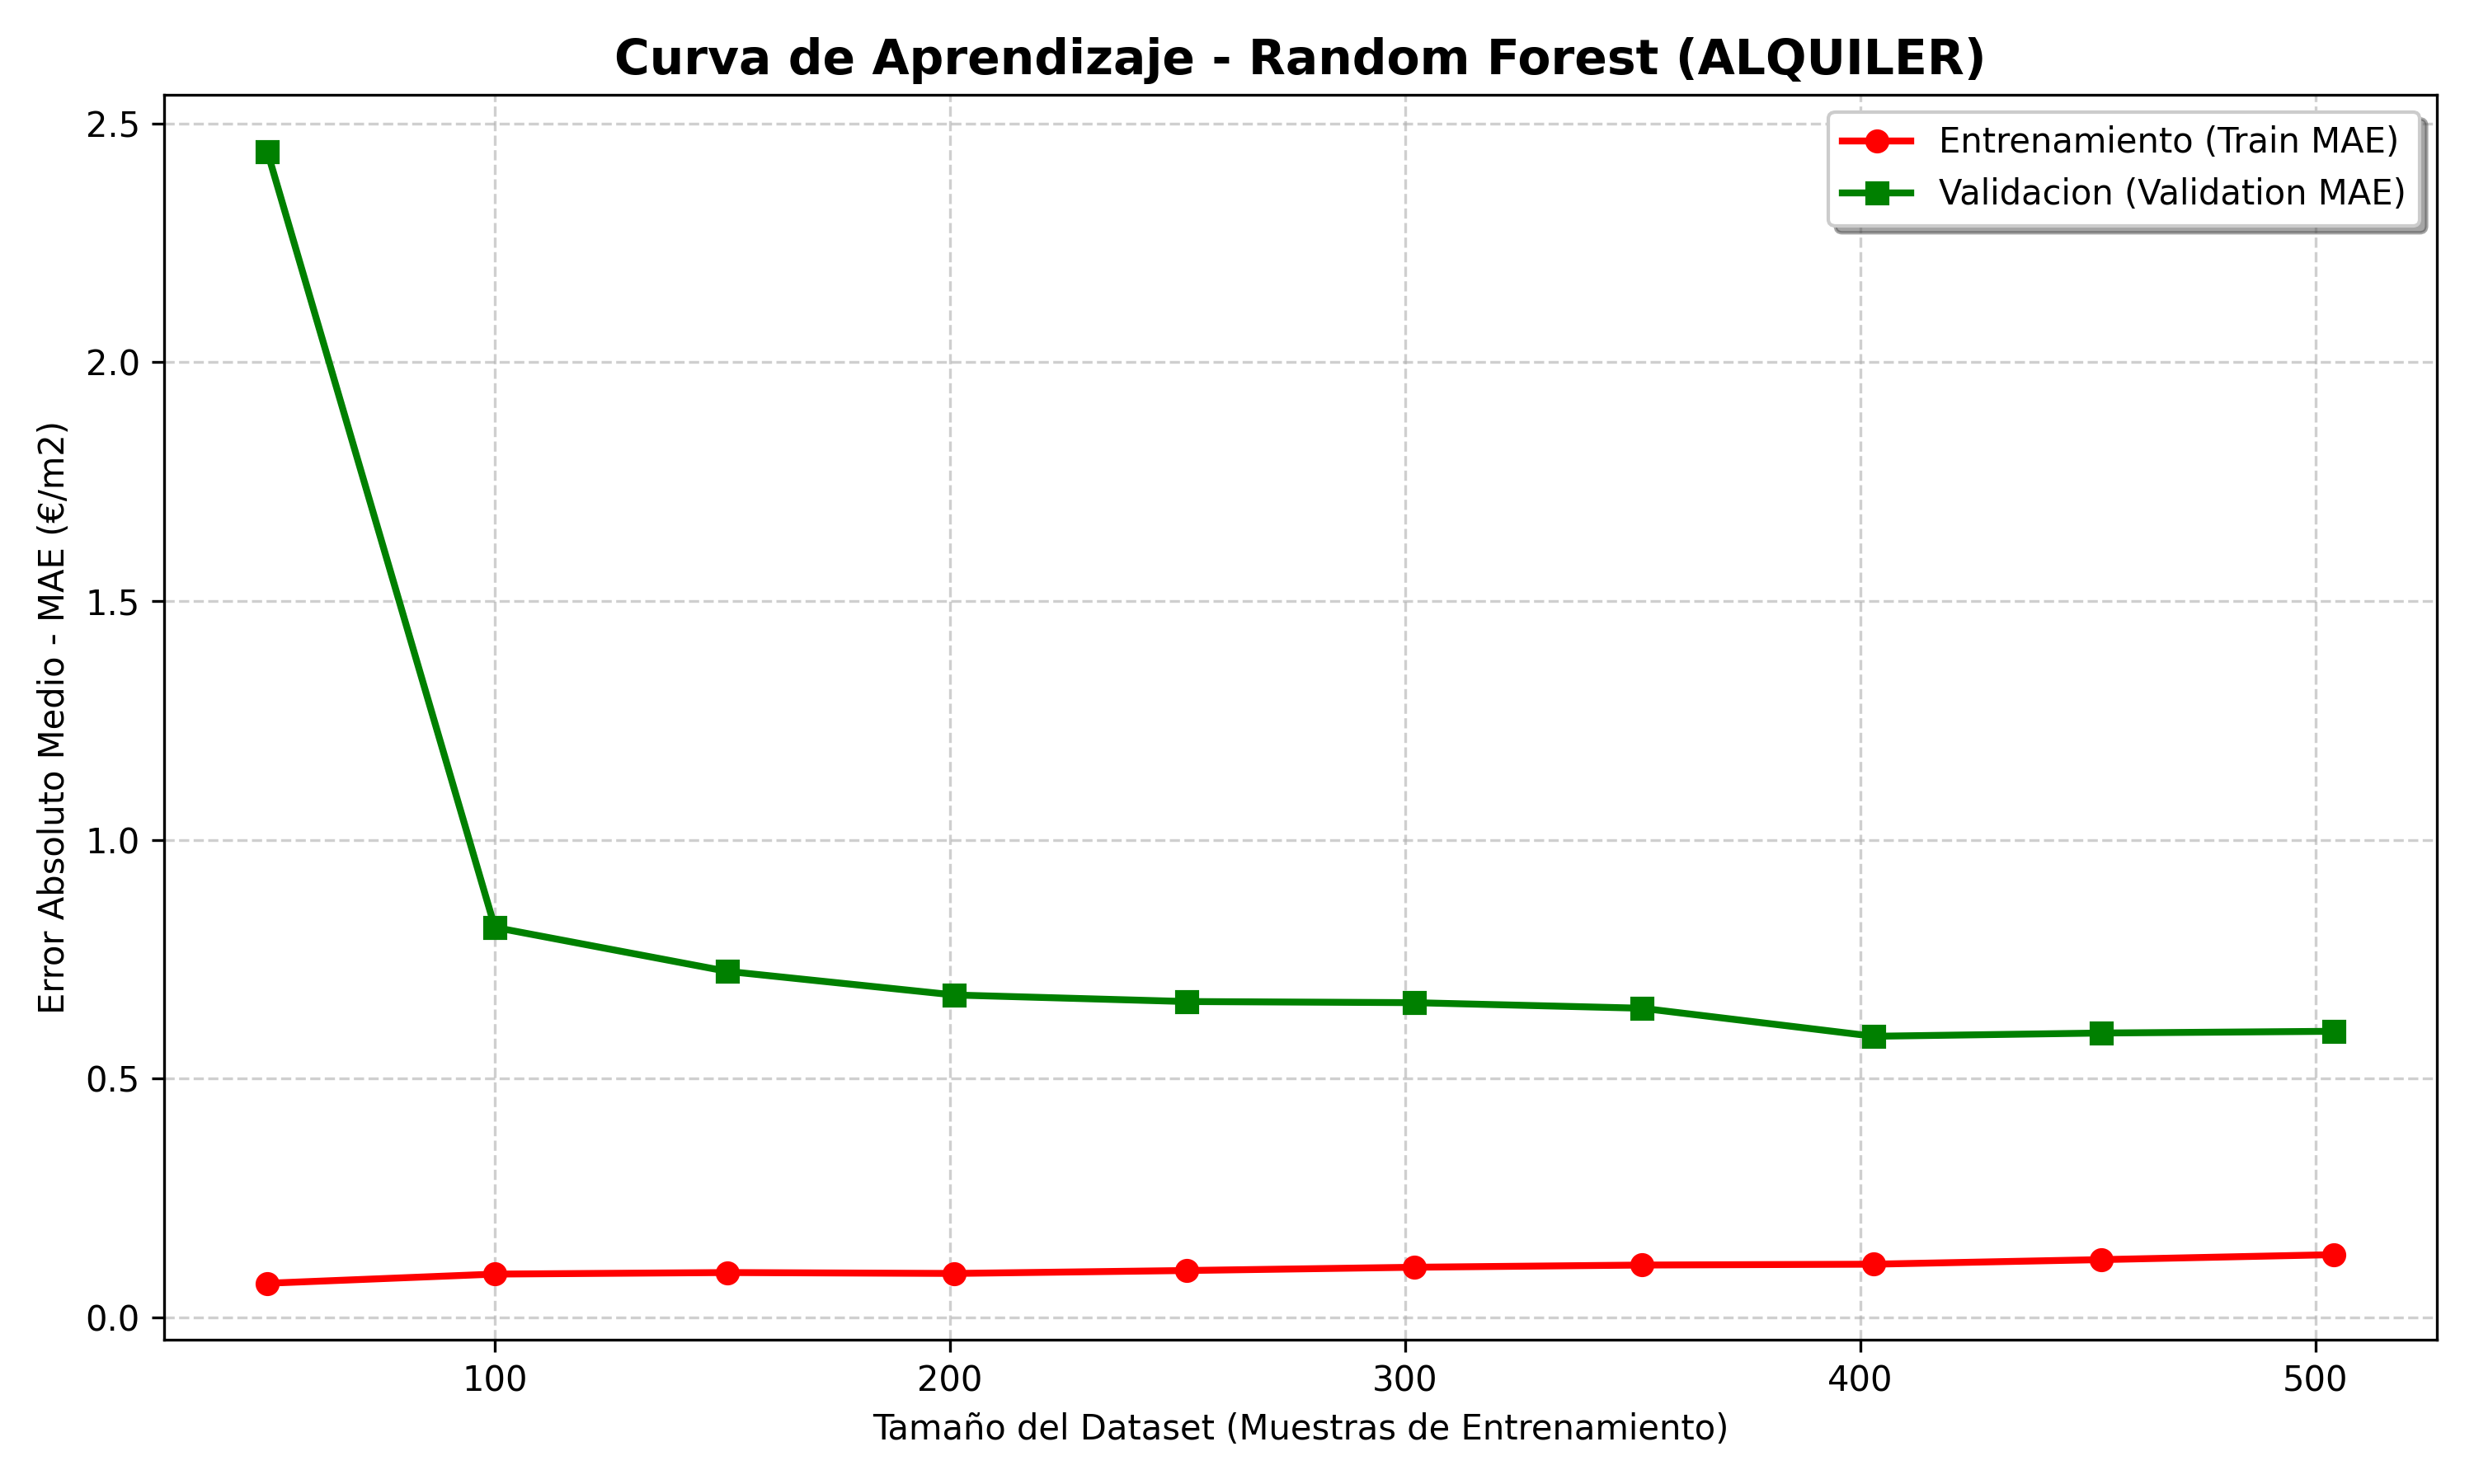
\includegraphics[width=0.40\linewidth]{img/phase1_learning_curve_random_forest_alquiler.png} \\
(a) Random Forest - Venta & (b) Random Forest - Alquiler \\
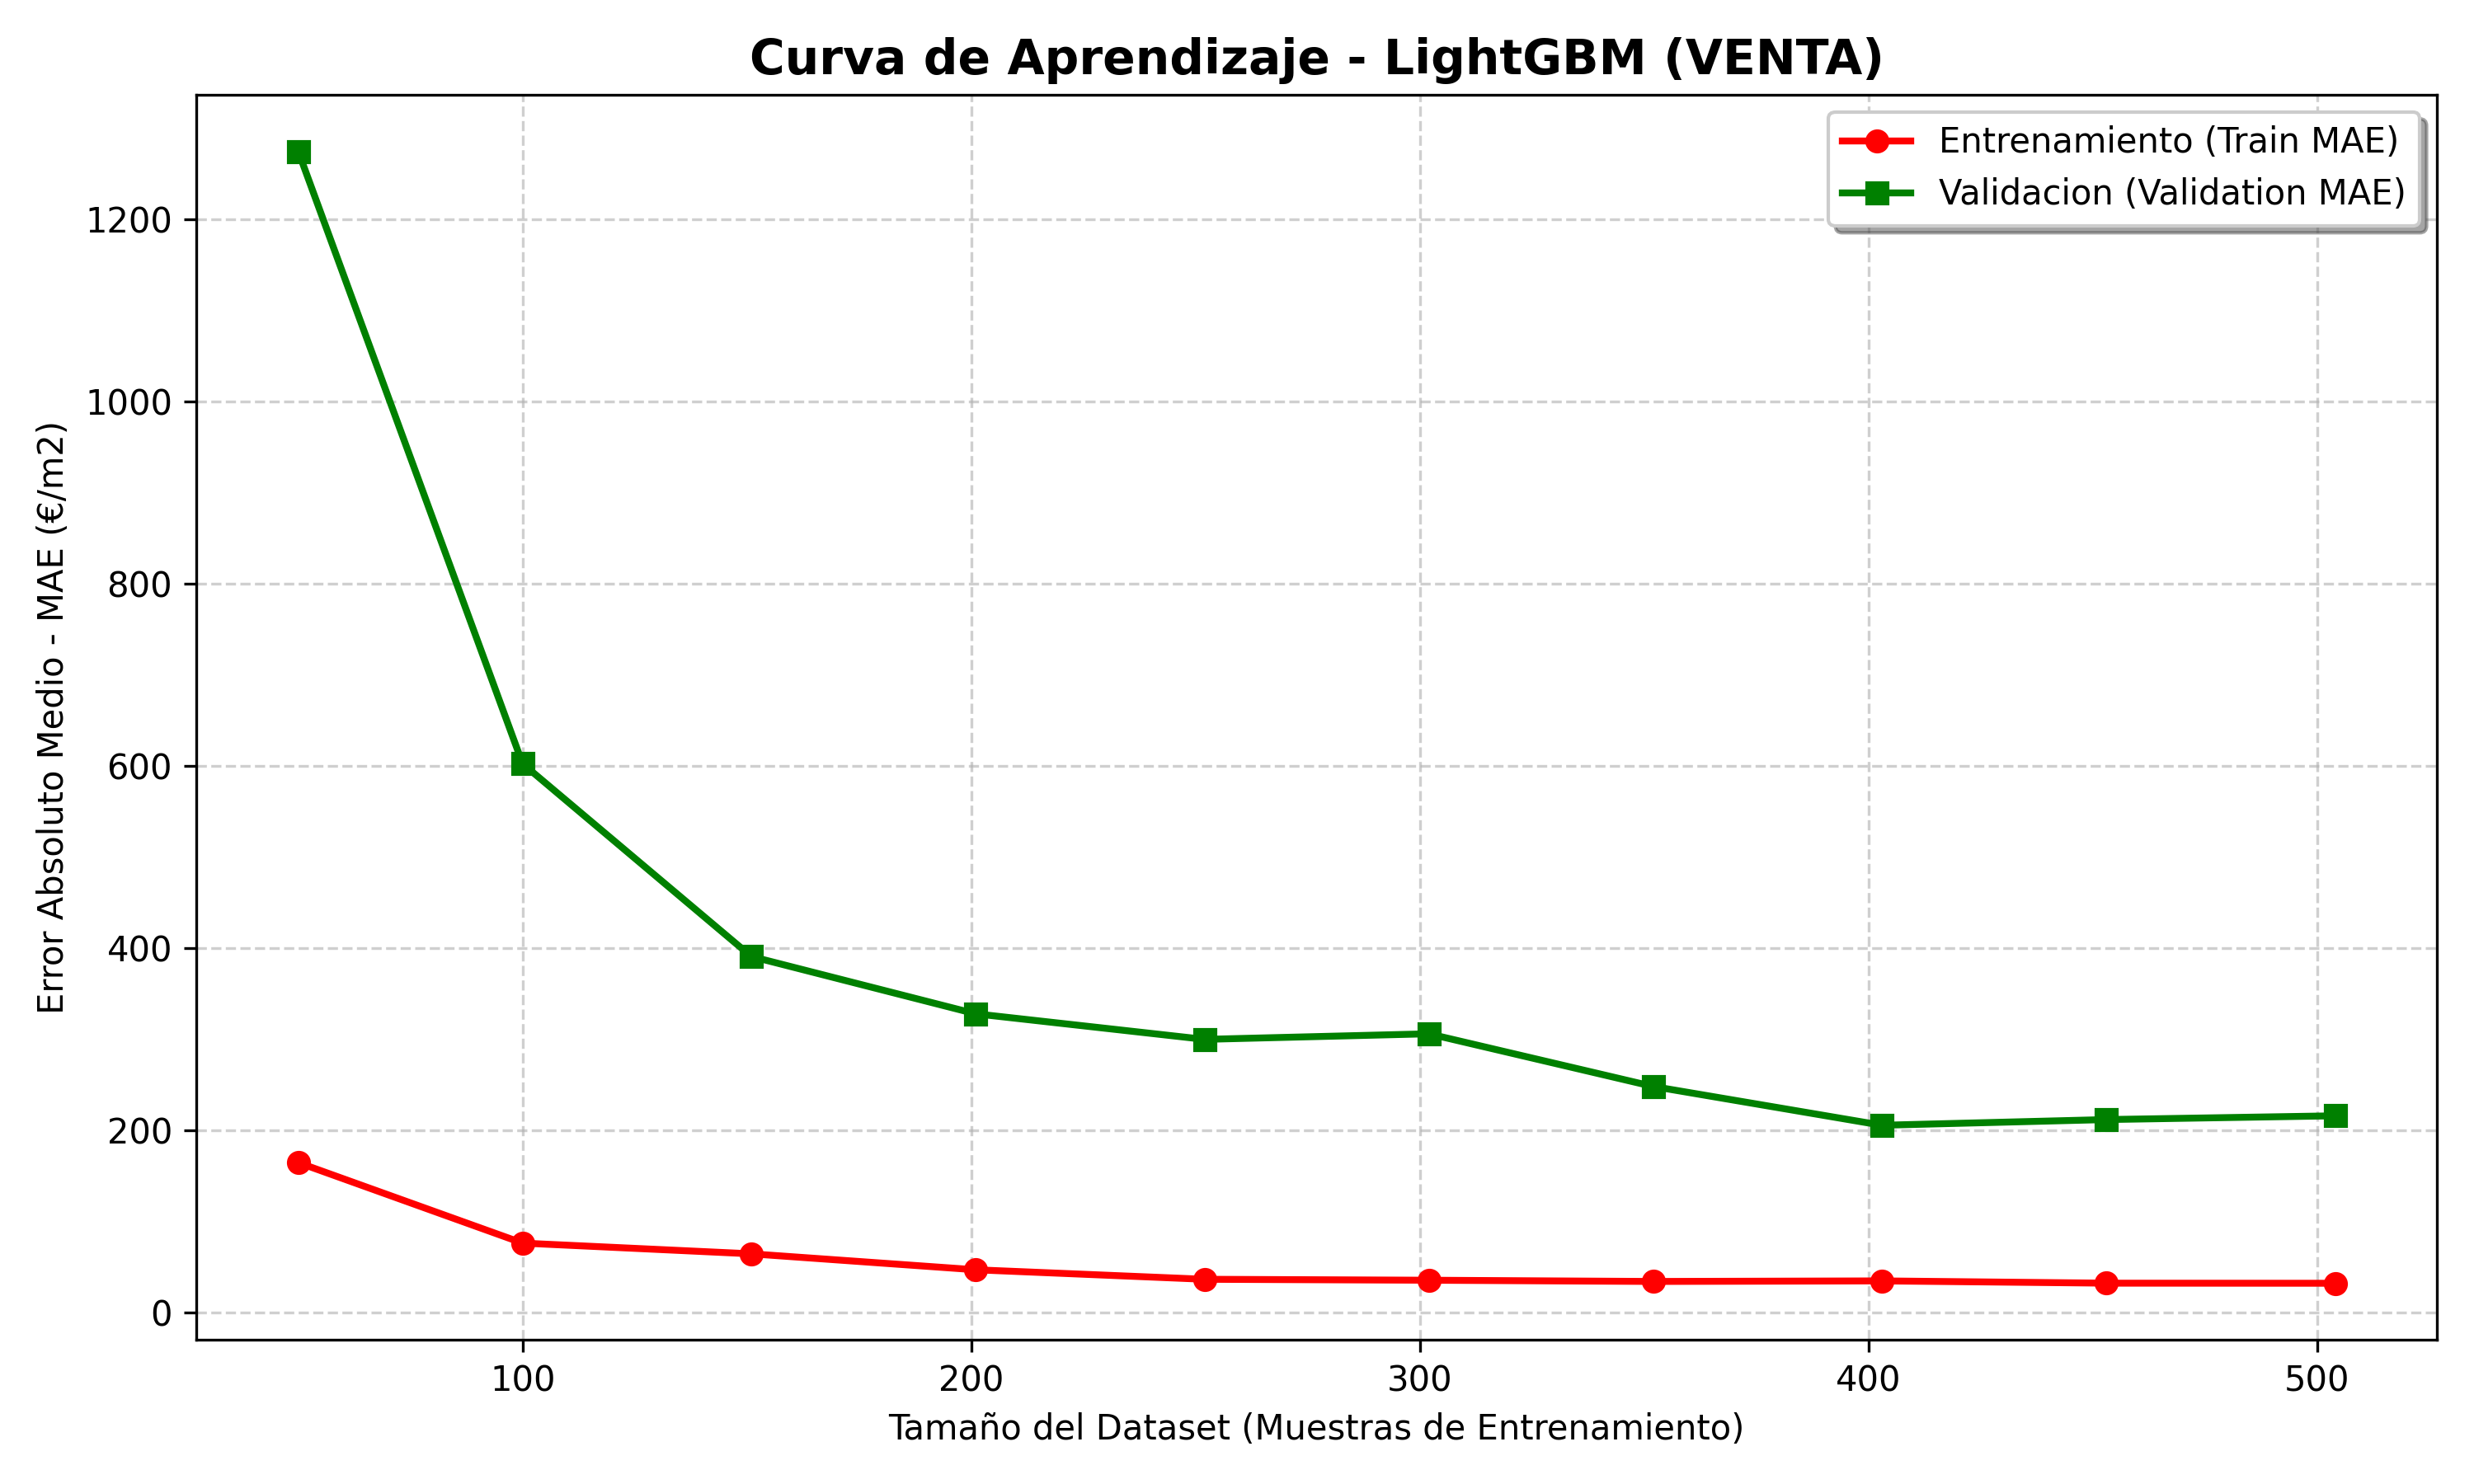
\includegraphics[width=0.40\linewidth]{img/phase1_learning_curve_lightgbm_venta.png} & 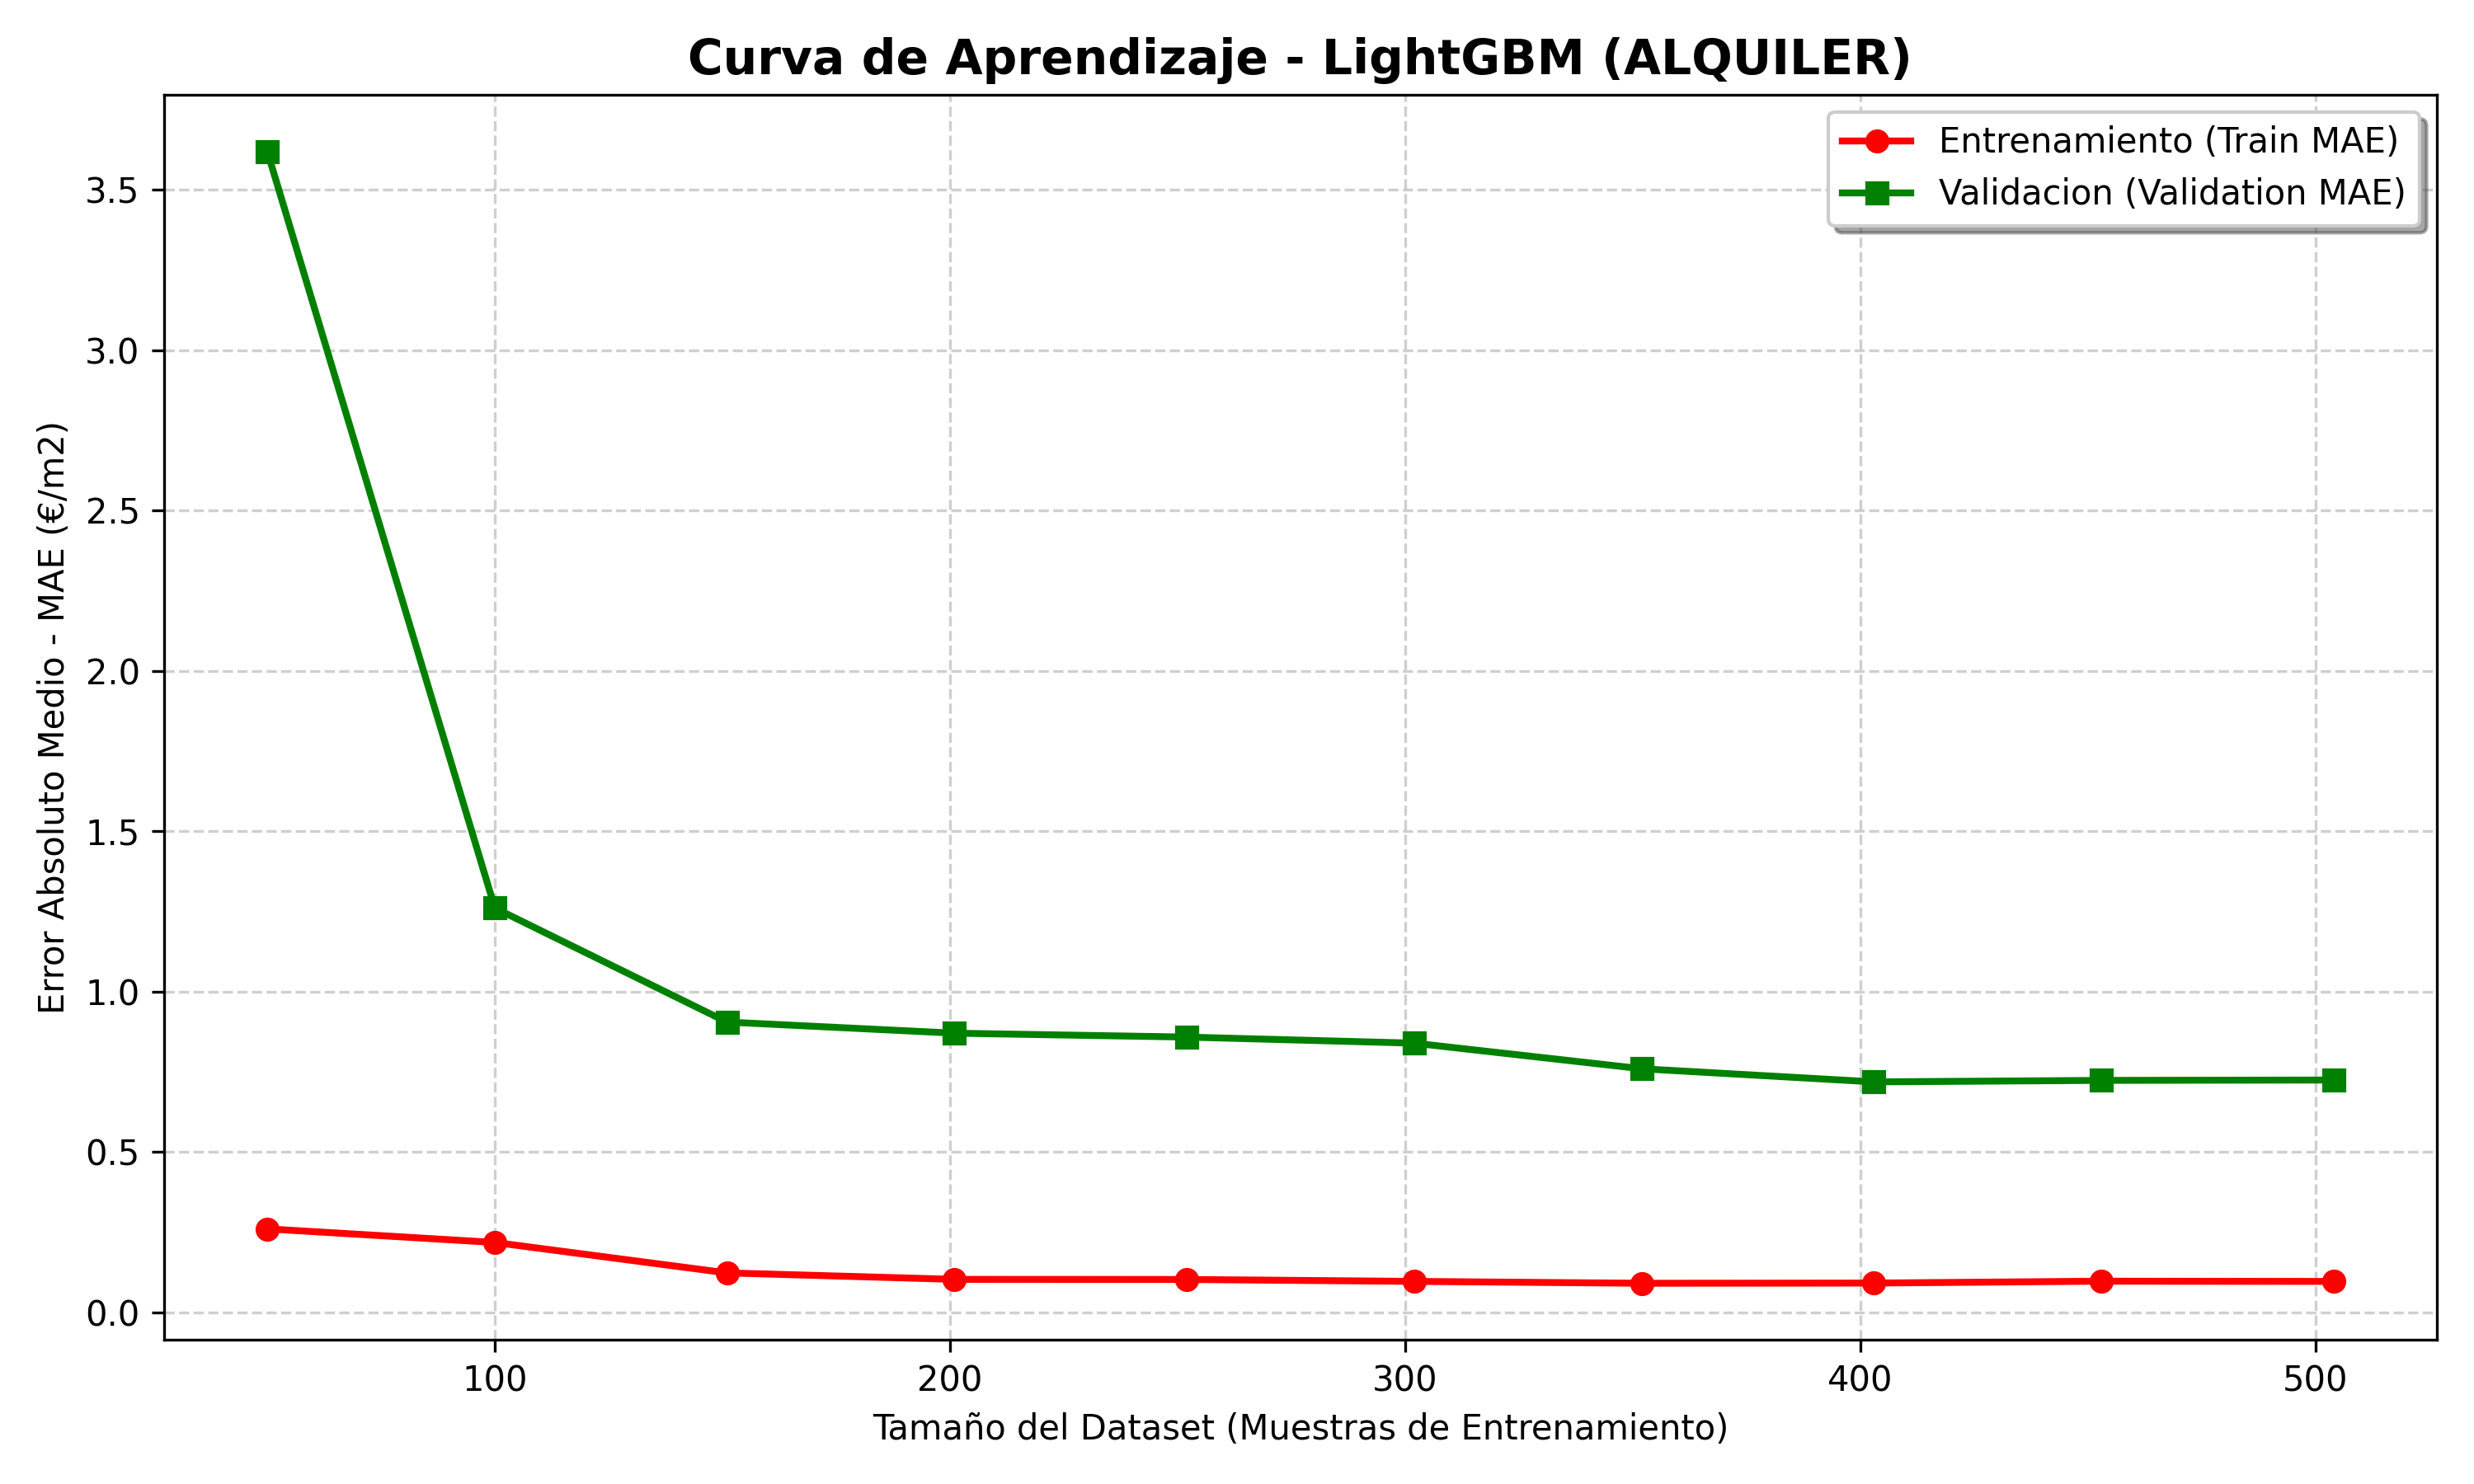
\includegraphics[width=0.40\linewidth]{img/phase1_learning_curve_lightgbm_alquiler.png} \\
(c) LightGBM - Venta & (d) LightGBM - Alquiler \\
\end{tabular}
\caption{Curvas de aprendizaje de Random Forest y LightGBM para los mercados de venta y alquiler en la Fase I.}
\label{fig:learning_curves_phase1_rf_lgb}
\end{figure}

\begin{figure}[H]
\centering
\begin{tabular}{cc}
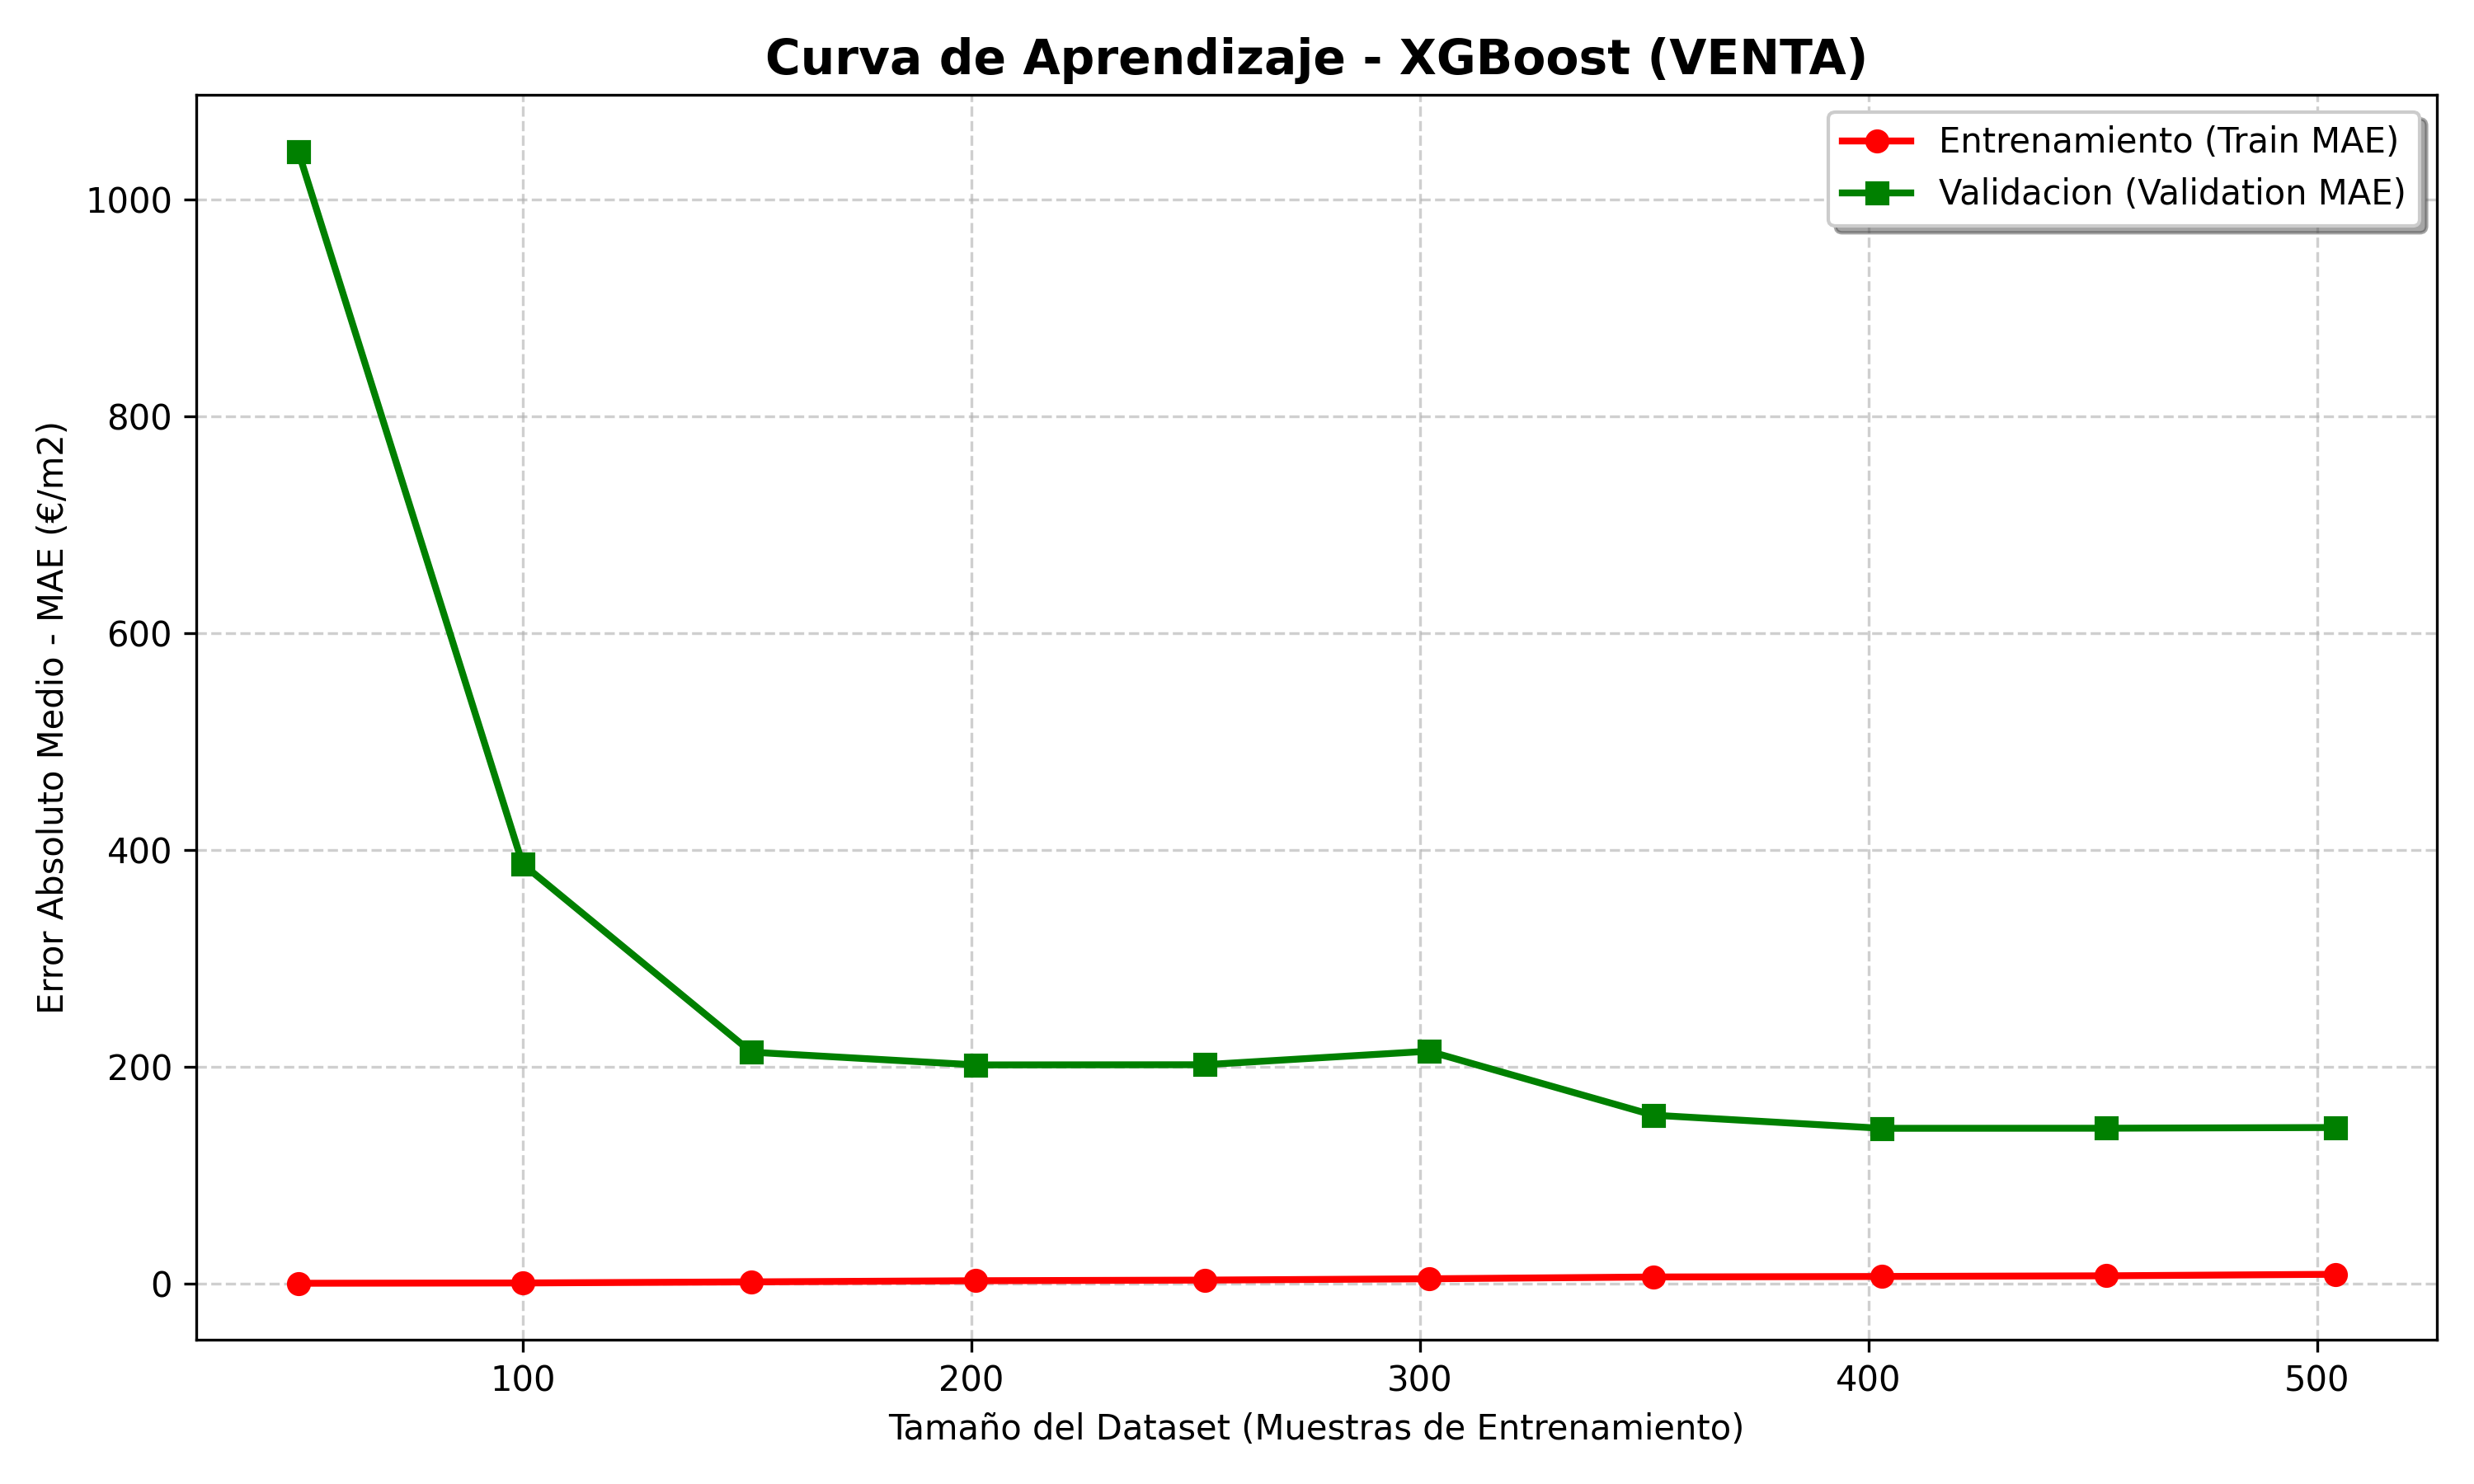
\includegraphics[width=0.40\linewidth]{img/phase1_learning_curve_xgboost_venta.png} & 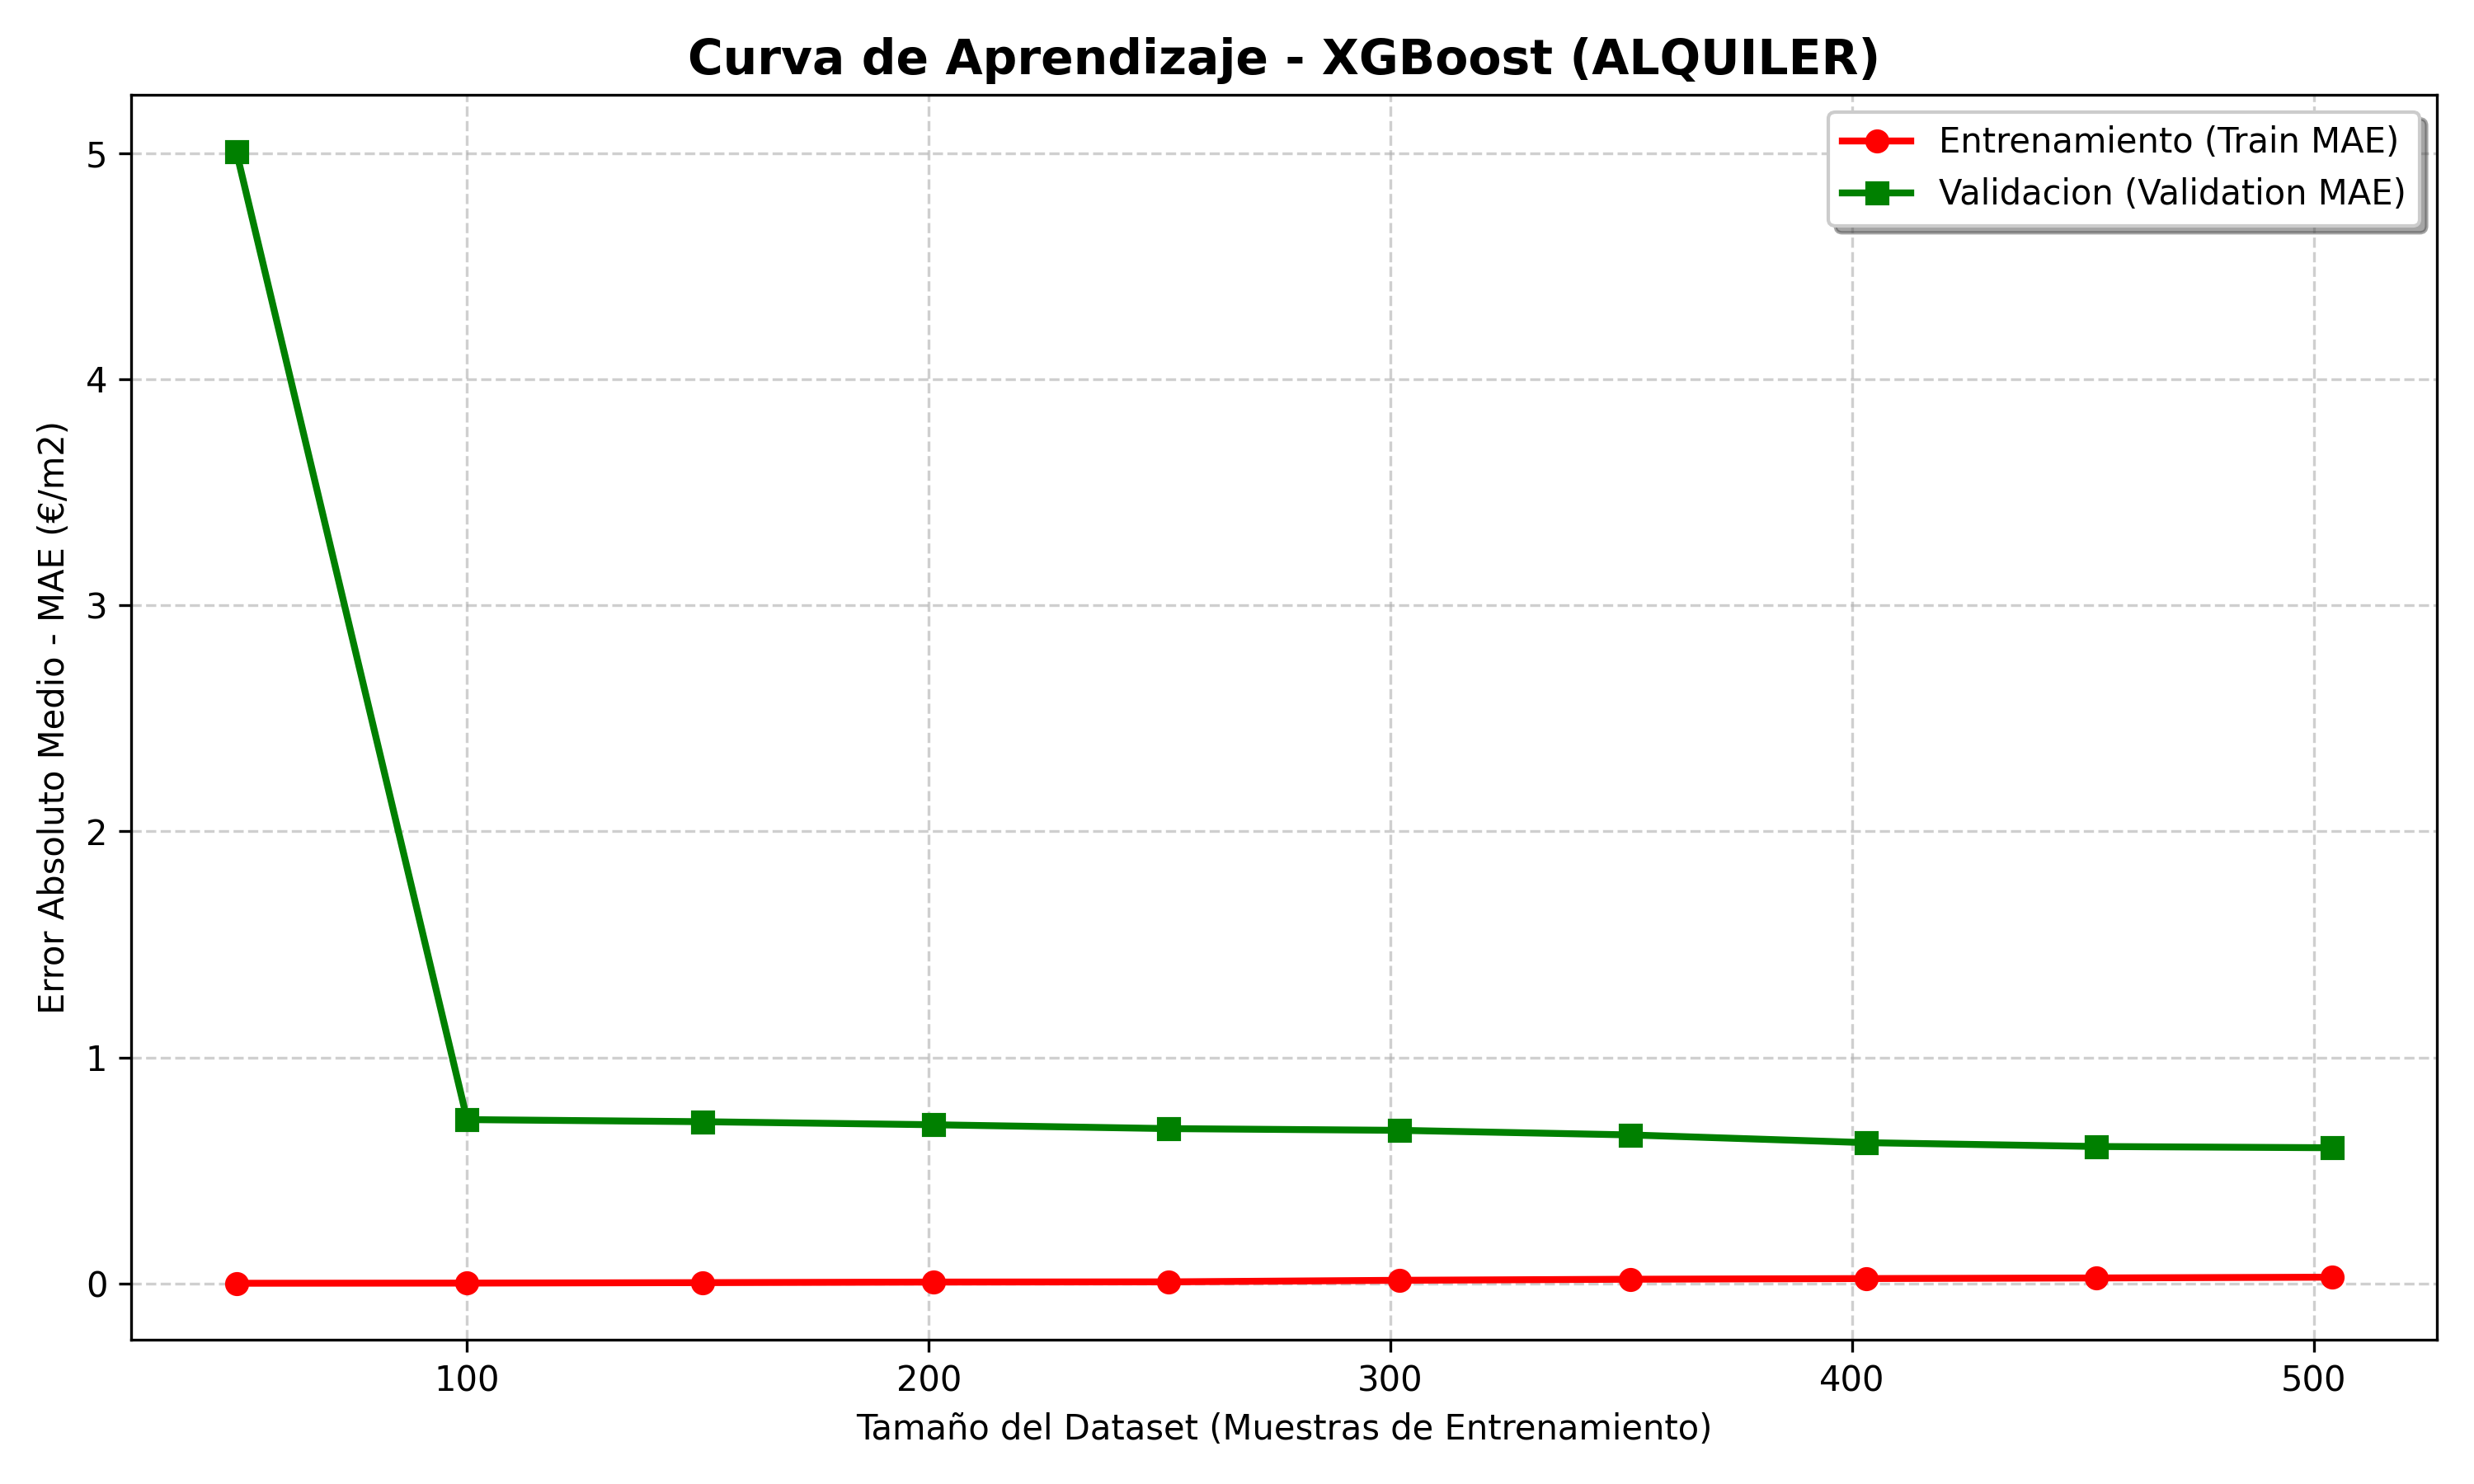
\includegraphics[width=0.40\linewidth]{img/phase1_learning_curve_xgboost_alquiler.png} \\
(a) XGBoost - Venta & (b) XGBoost - Alquiler \\
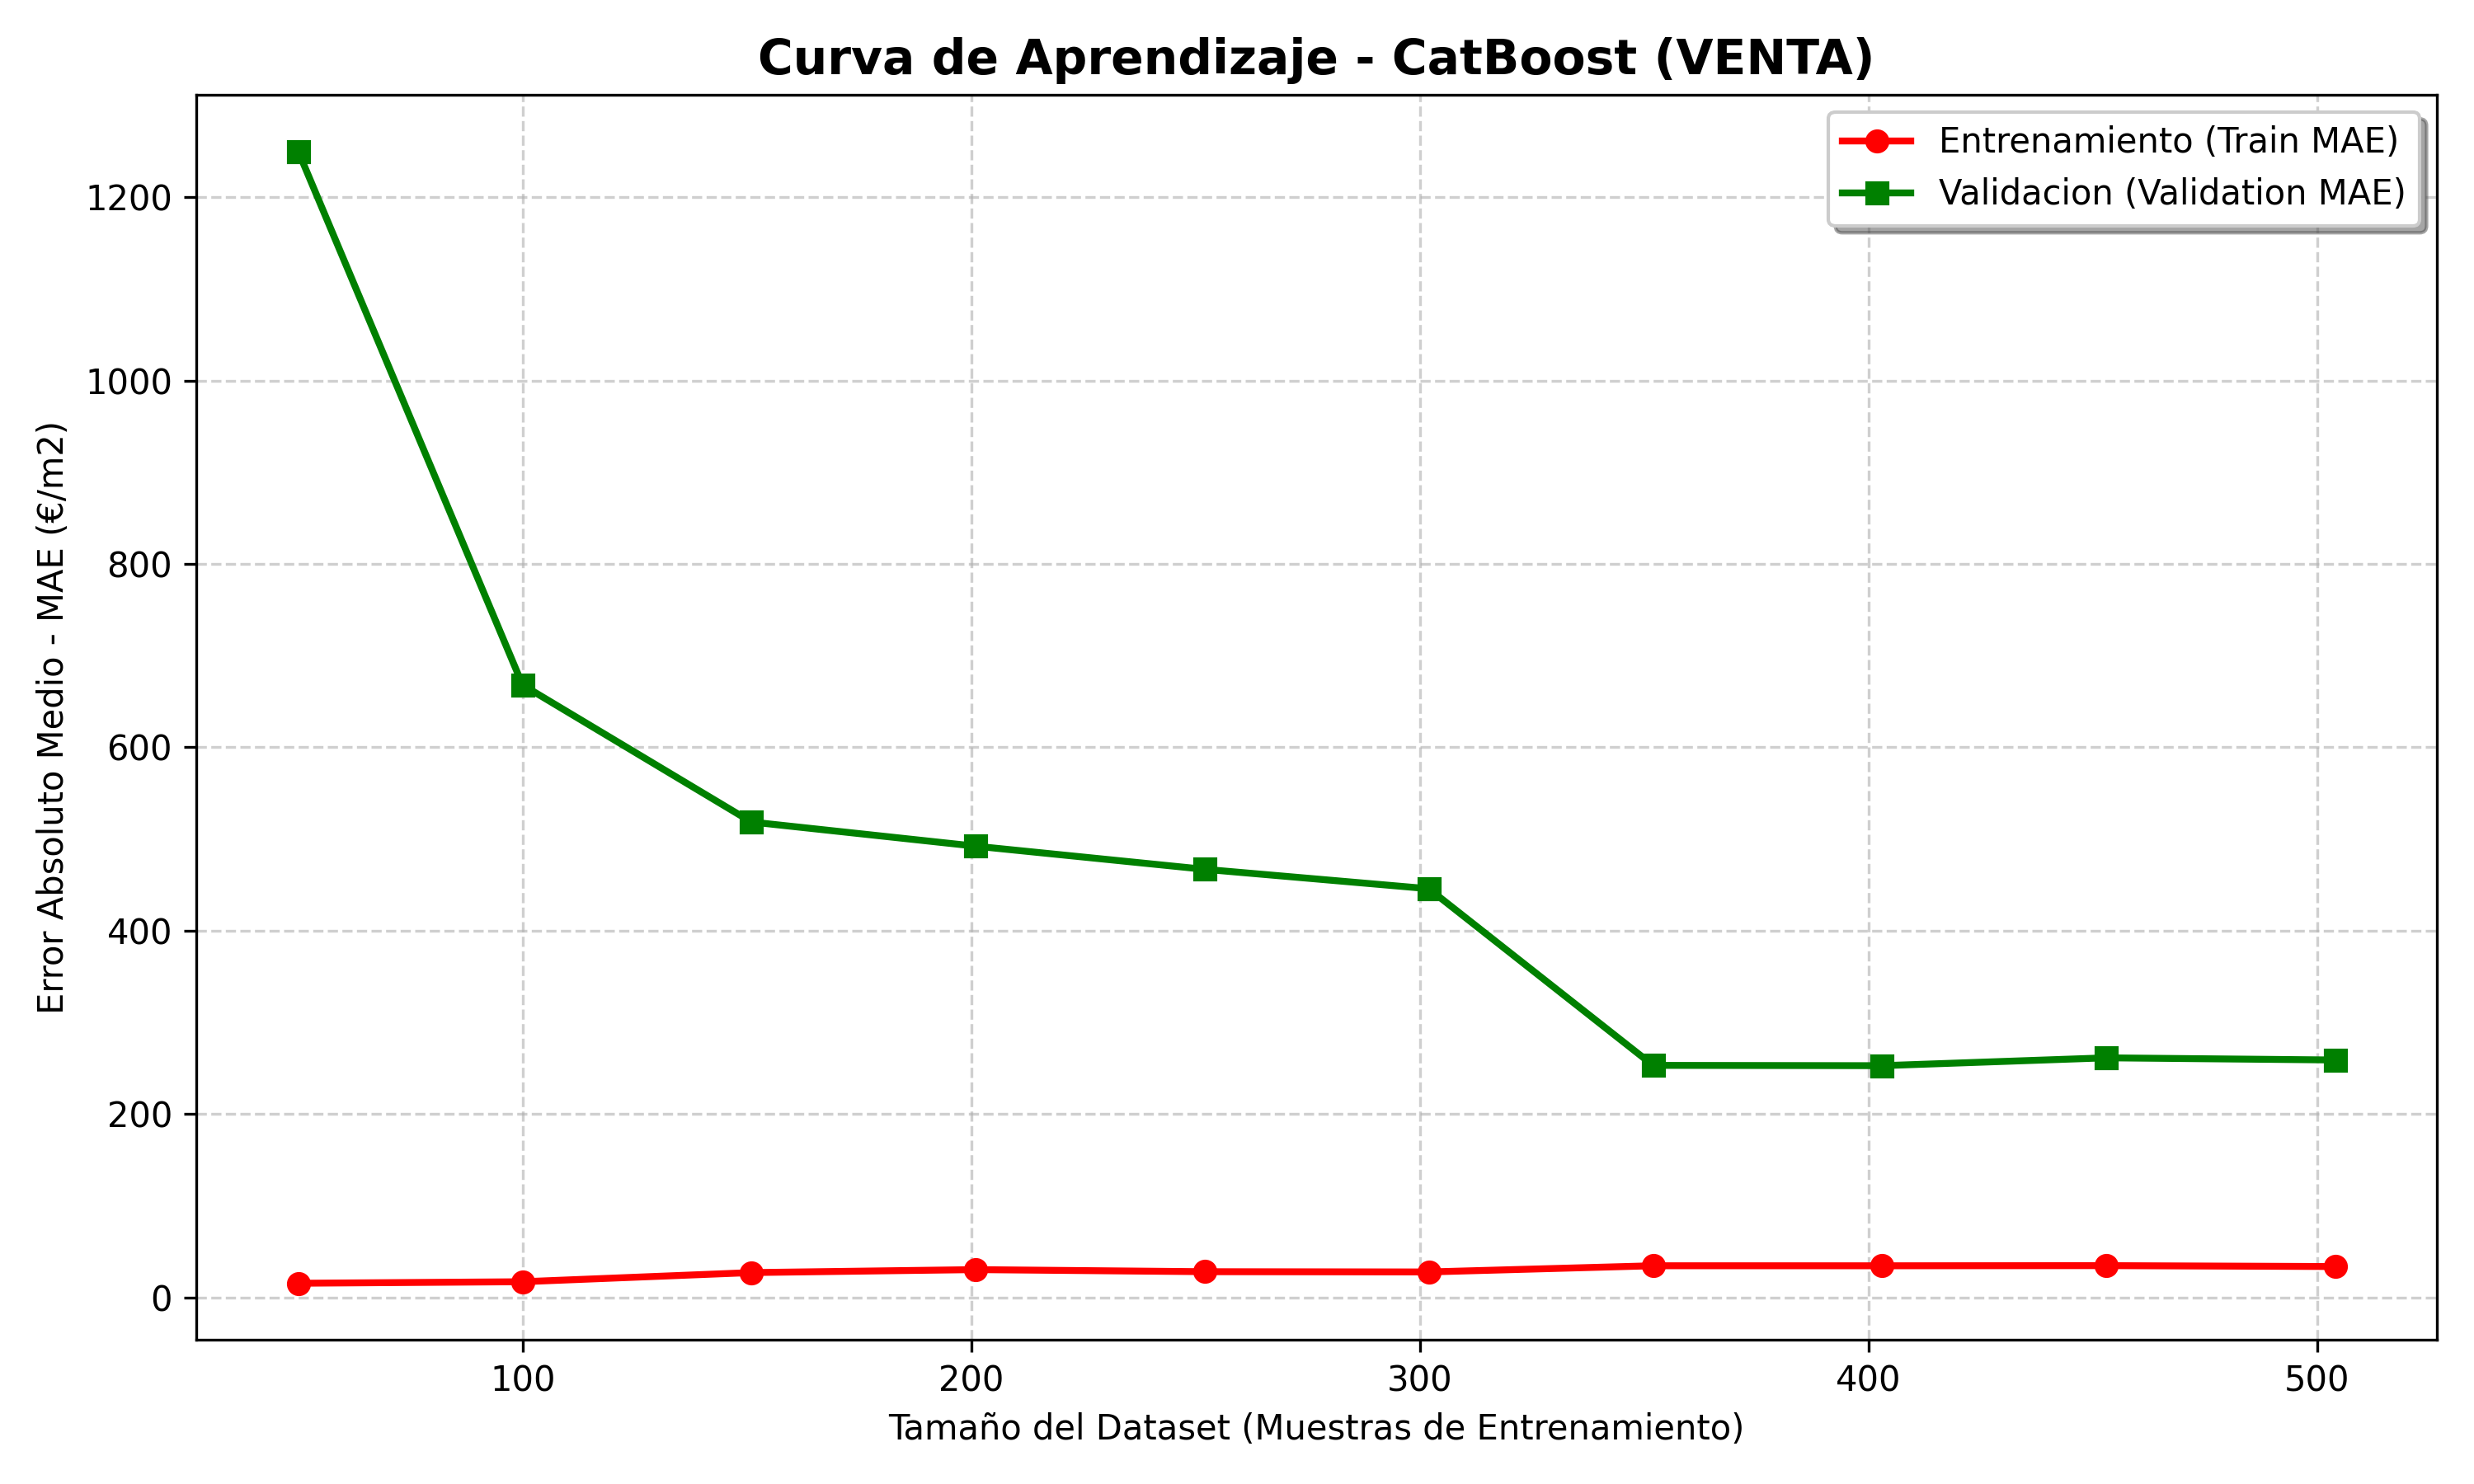
\includegraphics[width=0.40\linewidth]{img/phase1_learning_curve_catboost_venta.png} & 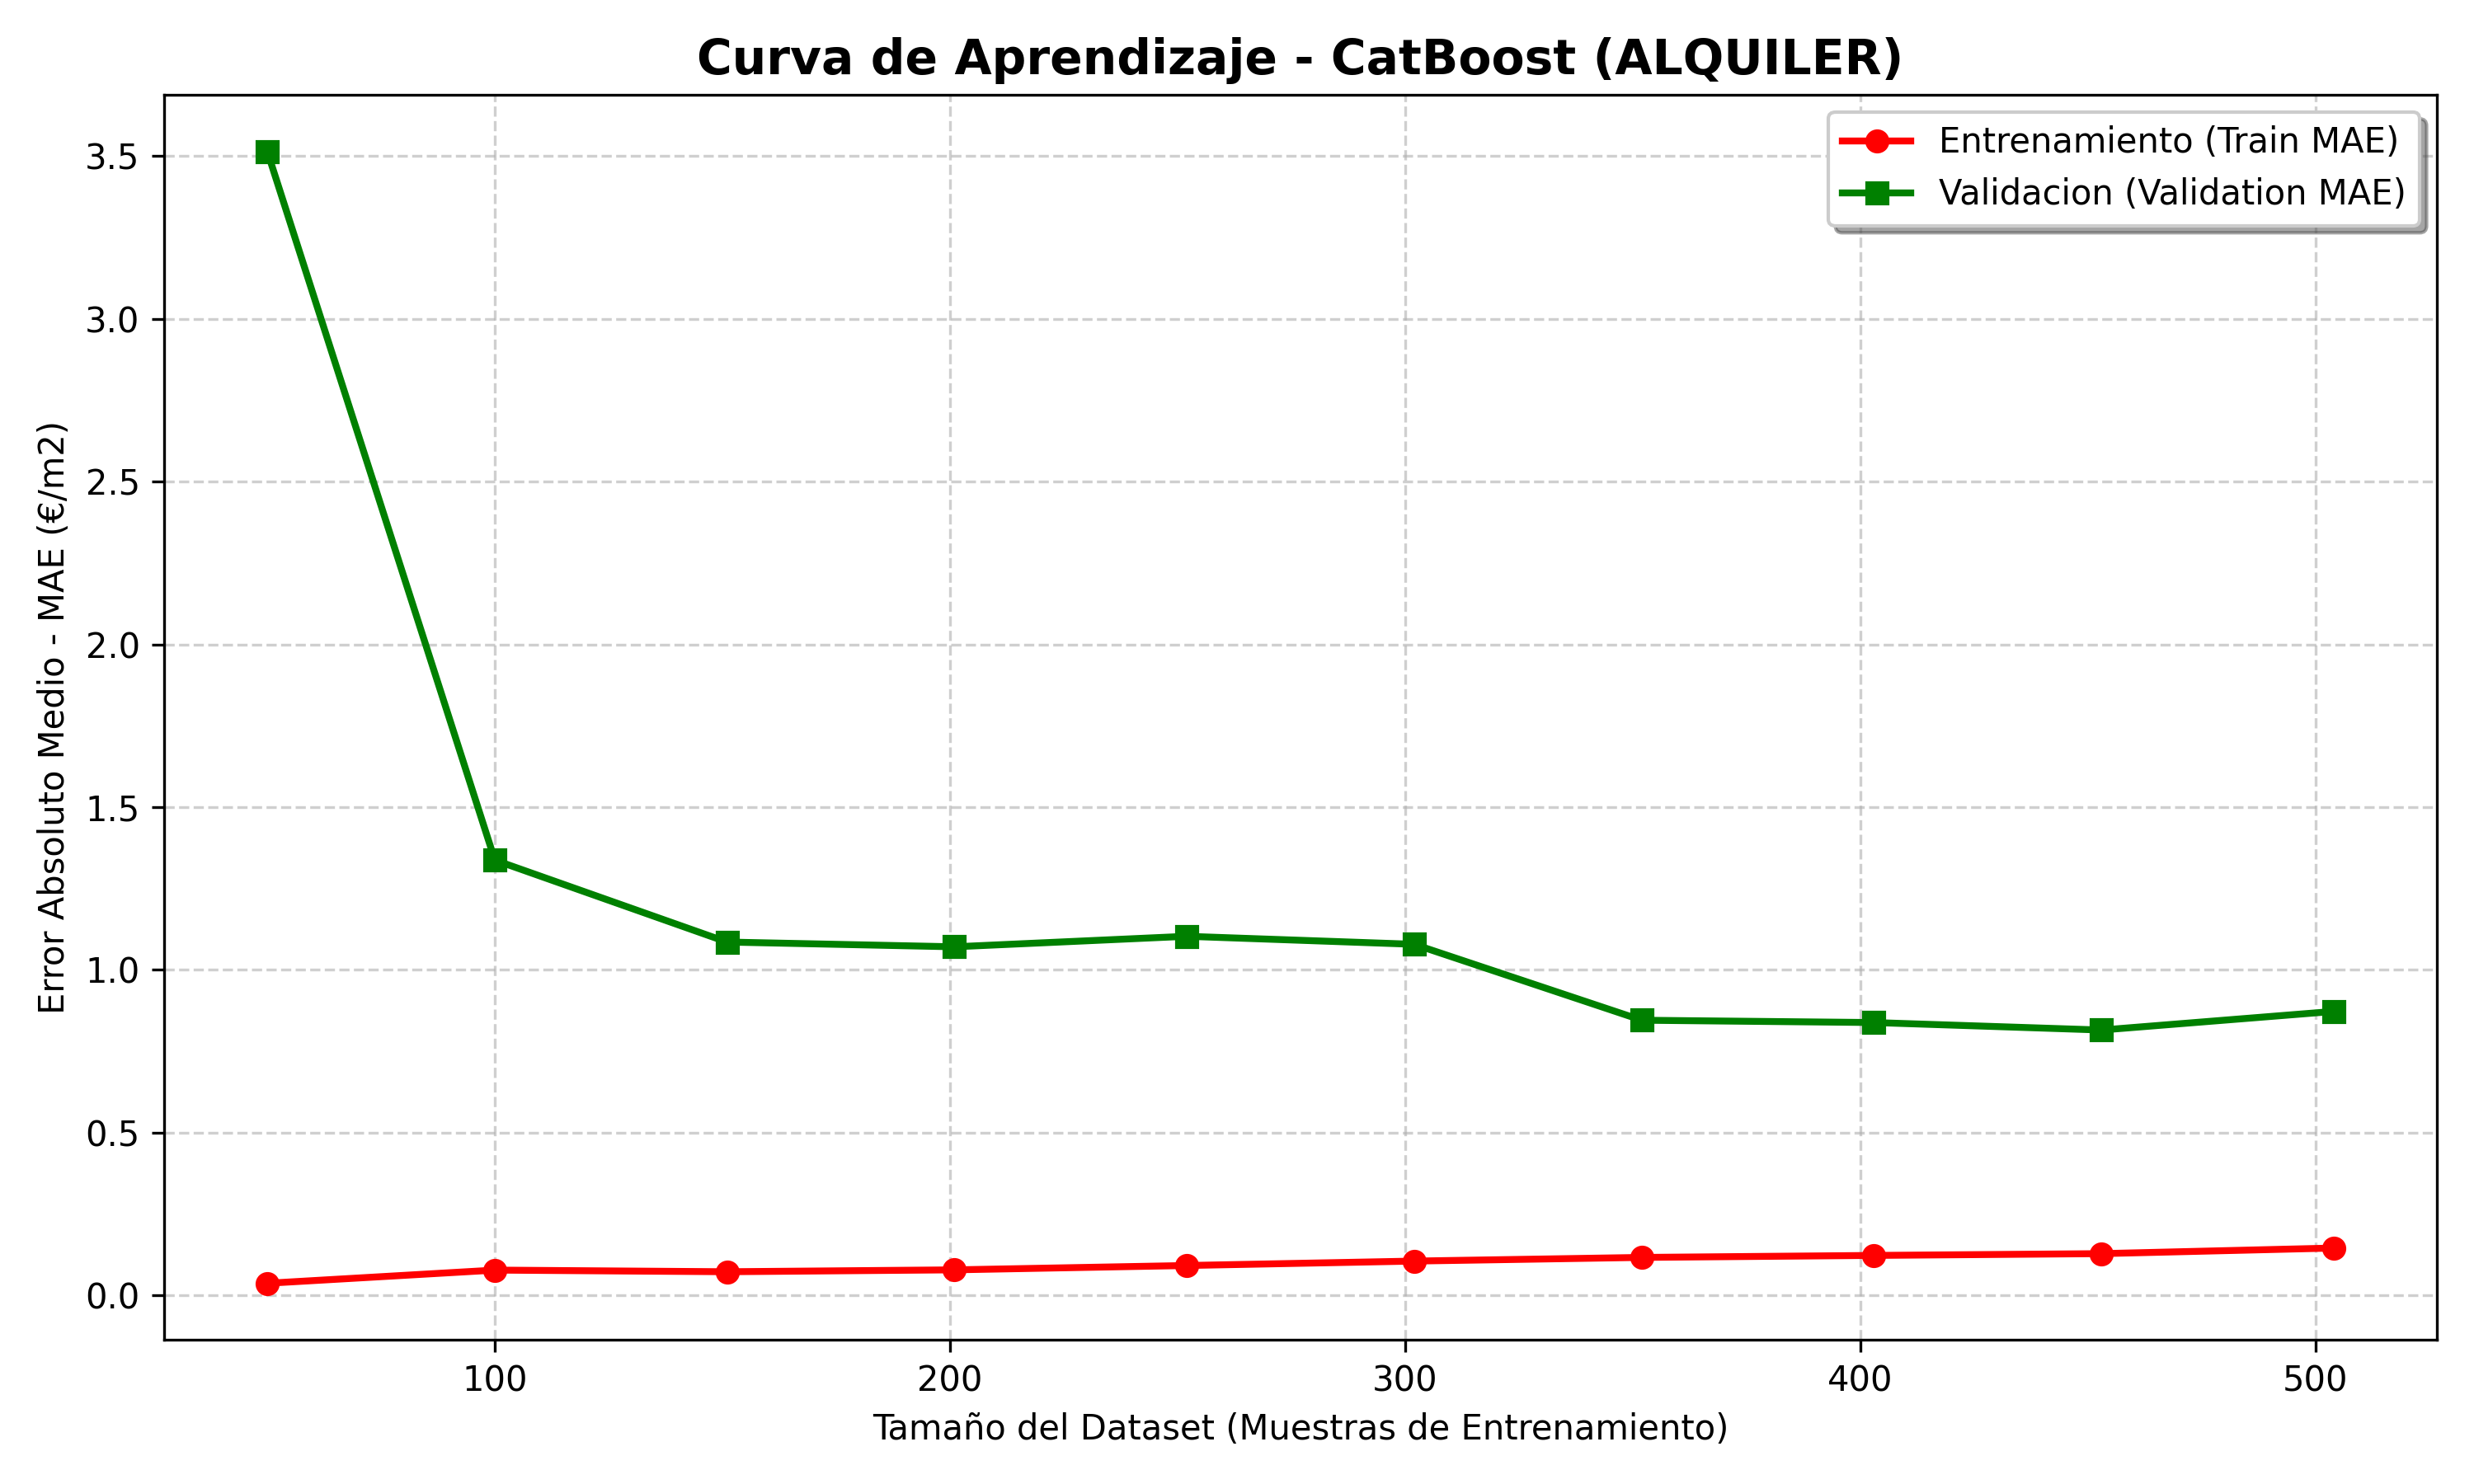
\includegraphics[width=0.40\linewidth]{img/phase1_learning_curve_catboost_alquiler.png} \\
(c) CatBoost - Venta & (d) CatBoost - Alquiler \\
\end{tabular}
\caption{Curvas de aprendizaje de XGBoost y CatBoost para los mercados de venta y alquiler en la Fase I.}
\label{fig:learning_curves_phase1_xgb_cat}
\end{figure}

\subsection{Alineación de Escalas Territoriales}
Una vez evaluado el comportamiento del modelo de distrito sobre barrios, la investigación se centró en analizar la influencia de la granularidad y la escala espacial en las estimaciones. La justificación teórica de esta experimentación se fundamenta en la literatura científica reciente sobre econometría espacial y modelado predictivo urbano. En particular, estudios clave como el publicado en el \textit{ISPRS International Journal of Geo-Information} (2025) sobre predicción de precios fine-grained frente a coarse-grained demuestran que los modelos desagregados (fine-grained) capturan de forma mucho más precisa el impacto de las instalaciones locales en el precio del suelo que los modelos agregados a gran escala (coarse-grained). Asimismo, trabajos sobre bases de datos espaciotemporales de vivienda en revistas de referencia como \textit{Scientific Data} (2026) constatan que algoritmos como XGBoost y LightGBM logran una mayor consistencia predictiva cuando se alimentan con granularidades micro-locales. Finalmente, la comparación sistemática entre modelos globales y locales en la literatura estadística (Cheng \& Ma, 2025) resalta que la escala geográfica de validación debe alinearse estrictamente con la de entrenamiento para evitar distorsiones de varianza espacial. Para analizar este comportamiento empíricamente, se entrenaron y evaluaron los regresores bajo dos aproximaciones de escala territorial bien diferenciadas, en ambas con retardos temporales.

\subsubsection{Alineación de Escalas Territoriales a Nivel de Barrio}
Para resolver la distorsión geográfica de la evaluación cruzada, esta etapa de la investigación centró el modelado en una escala micro-local homogénea. Al entrenar y evaluar los modelos exclusivamente a escala de barrio (\texttt{id\_barrio != -1}) con los retardos dinámicos inyectados, el error se redujo sustancialmente, lo que permitió lograr una precisión excepcional tanto a nivel global como local. Como se expone en la Tabla~\ref{tab:phase2_barrio_venta} y la Tabla~\ref{tab:phase2_barrio_alquiler}, los regresores asimilan de forma óptima el gradiente territorial micro-local y los patrones espaciales reales.

\begin{table}[H]
\centering
\caption{Matriz de rendimiento comparativa: Alineación de escalas a nivel micro-local de barrio con retardos temporales - Mercado de Venta (€/m\textsuperscript{2})}
\label{tab:phase2_barrio_venta}
\resizebox{\textwidth}{!}{%
\begin{tabular}{|l|c|c|c|c|c|c|c|c|c|c|c|}
\hline
\textbf{Algoritmo} & \textbf{MAE} & \textbf{RMSE} & \textbf{R\textsuperscript{2}} & \textbf{MAPE} & \textbf{Sesgo} & \textbf{MAE} & \textbf{R\textsuperscript{2}} & \textbf{MAE} & \textbf{R\textsuperscript{2}} & \textbf{T. Train} & \textbf{T. Pred} \\
 & \textbf{Global} & \textbf{Global} & \textbf{Global} & \textbf{Global (\%)} & \textbf{Global} & \textbf{Salamanca} & \textbf{Salamanca} & \textbf{C. Lineal} & \textbf{C. Lineal} & \textbf{(s)} & \textbf{(s)} \\
\hline
\textbf{Random Forest} & \textbf{100,50} & \textbf{136,82} & \textbf{0,9956} & \textbf{1,87\%} & 38,59 & 122,34 & 0,9646 & \textbf{130,04} & \textbf{0,9882} & 0,601 & 0,055 \\
\textbf{CatBoost} & 128,24 & 186,36 & 0,9919 & 2,38\% & -16,97 & 133,76 & 0,9657 & 283,50 & 0,9451 & 0,733 & \textbf{0,002} \\
\textbf{XGBoost} & 111,67 & 153,66 & 0,9945 & 2,11\% & \textbf{7,39} & \textbf{88,40} & \textbf{0,9686} & 182,94 & 0,9779 & 0,391 & 0,005 \\
\textbf{LightGBM} & 115,47 & 156,80 & 0,9943 & 2,10\% & 22,34 & 110,90 & 0,9623 & 230,19 & 0,9702 & \textbf{0,462} & 0,003 \\
\hline
\end{tabular}%
}
\end{table}

\begin{table}[H]
\centering
\caption{Matriz de rendimiento comparativa: Alineación de escalas a nivel micro-local de barrio con retardos temporales - Mercado de Alquiler (€/m\textsuperscript{2})}
\label{tab:phase2_barrio_alquiler}
\resizebox{\textwidth}{!}{%
\begin{tabular}{|l|c|c|c|c|c|c|c|c|c|c|c|}
\hline
\textbf{Algoritmo} & \textbf{MAE} & \textbf{RMSE} & \textbf{R\textsuperscript{2}} & \textbf{MAPE} & \textbf{Sesgo} & \textbf{MAE} & \textbf{R\textsuperscript{2}} & \textbf{MAE} & \textbf{R\textsuperscript{2}} & \textbf{T. Train} & \textbf{T. Pred} \\
 & \textbf{Global} & \textbf{Global} & \textbf{Global} & \textbf{Global (\%)} & \textbf{Global} & \textbf{Salamanca} & \textbf{Salamanca} & \textbf{C. Lineal} & \textbf{C. Lineal} & \textbf{(s)} & \textbf{(s)} \\
\hline
\textbf{Random Forest} & \textbf{0,454} & \textbf{0,596} & \textbf{0,9762} & \textbf{2,21\%} & 0,023 & \textbf{0,434} & \textbf{0,7752} & \textbf{0,516} & \textbf{0,9688} & 0,578 & 0,055 \\
\textbf{CatBoost} & 0,502 & 0,651 & 0,9716 & 2,39\% & \textbf{-0,013} & 0,578 & 0,7012 & 0,795 & 0,9186 & 0,535 & \textbf{0,001} \\
\textbf{XGBoost} & 0,510 & 0,665 & 0,9704 & 2,45\% & -0,112 & 0,550 & 0,6101 & 0,674 & 0,9287 & 0,358 & 0,005 \\
\textbf{LightGBM} & 0,503 & 0,650 & 0,9717 & 2,44\% & -0,065 & 0,493 & 0,7584 & 0,610 & 0,9405 & \textbf{0,280} & 0,004 \\
\hline
\end{tabular}%
}
\end{table}

Al analizar de forma comparativa los resultados del modelado micro-local a nivel de barrio expuestos en la Tabla~\ref{tab:phase2_barrio_venta} y la Tabla~\ref{tab:phase2_barrio_alquiler} frente al escenario previo de evaluación cruzada, se observa una disminución general del error predictivo global en todos los algoritmos analizados, tanto para el mercado de venta como para el de alquiler. En el mercado de venta, el MAE global de Random Forest desciende a 100,50 \text{€/m\textsuperscript{2}} y el de XGBoost se sitúa en 111,67 \text{€/m\textsuperscript{2}} (frente a los 152,83 y 143,81 \text{€/m\textsuperscript{2}} de la evaluación cruzada), lo cual representa una ganancia neta en la precisión. En el mercado de alquiler, el error global disminuye notablemente, situándose en un MAE de 0,454 \text{€/m\textsuperscript{2}} para Random Forest y 0,503 \text{€/m\textsuperscript{2}} para LightGBM (frente a 0,599 y 0,724 \text{€/m\textsuperscript{2}} respectivamente en la evaluación cruzada). Esta mejora empírica confirma que entrenar y evaluar los estimadores dentro del mismo nivel de granularidad geográfica micro-local suprime las distorsiones de varianza espacial introducidas al proyectar modelos agregados sobre zonas heterogéneas, lo que dota a los algoritmos de una base espacial mucho más consistente.

\begin{figure}[H]
\centering
\begin{tabular}{cc}
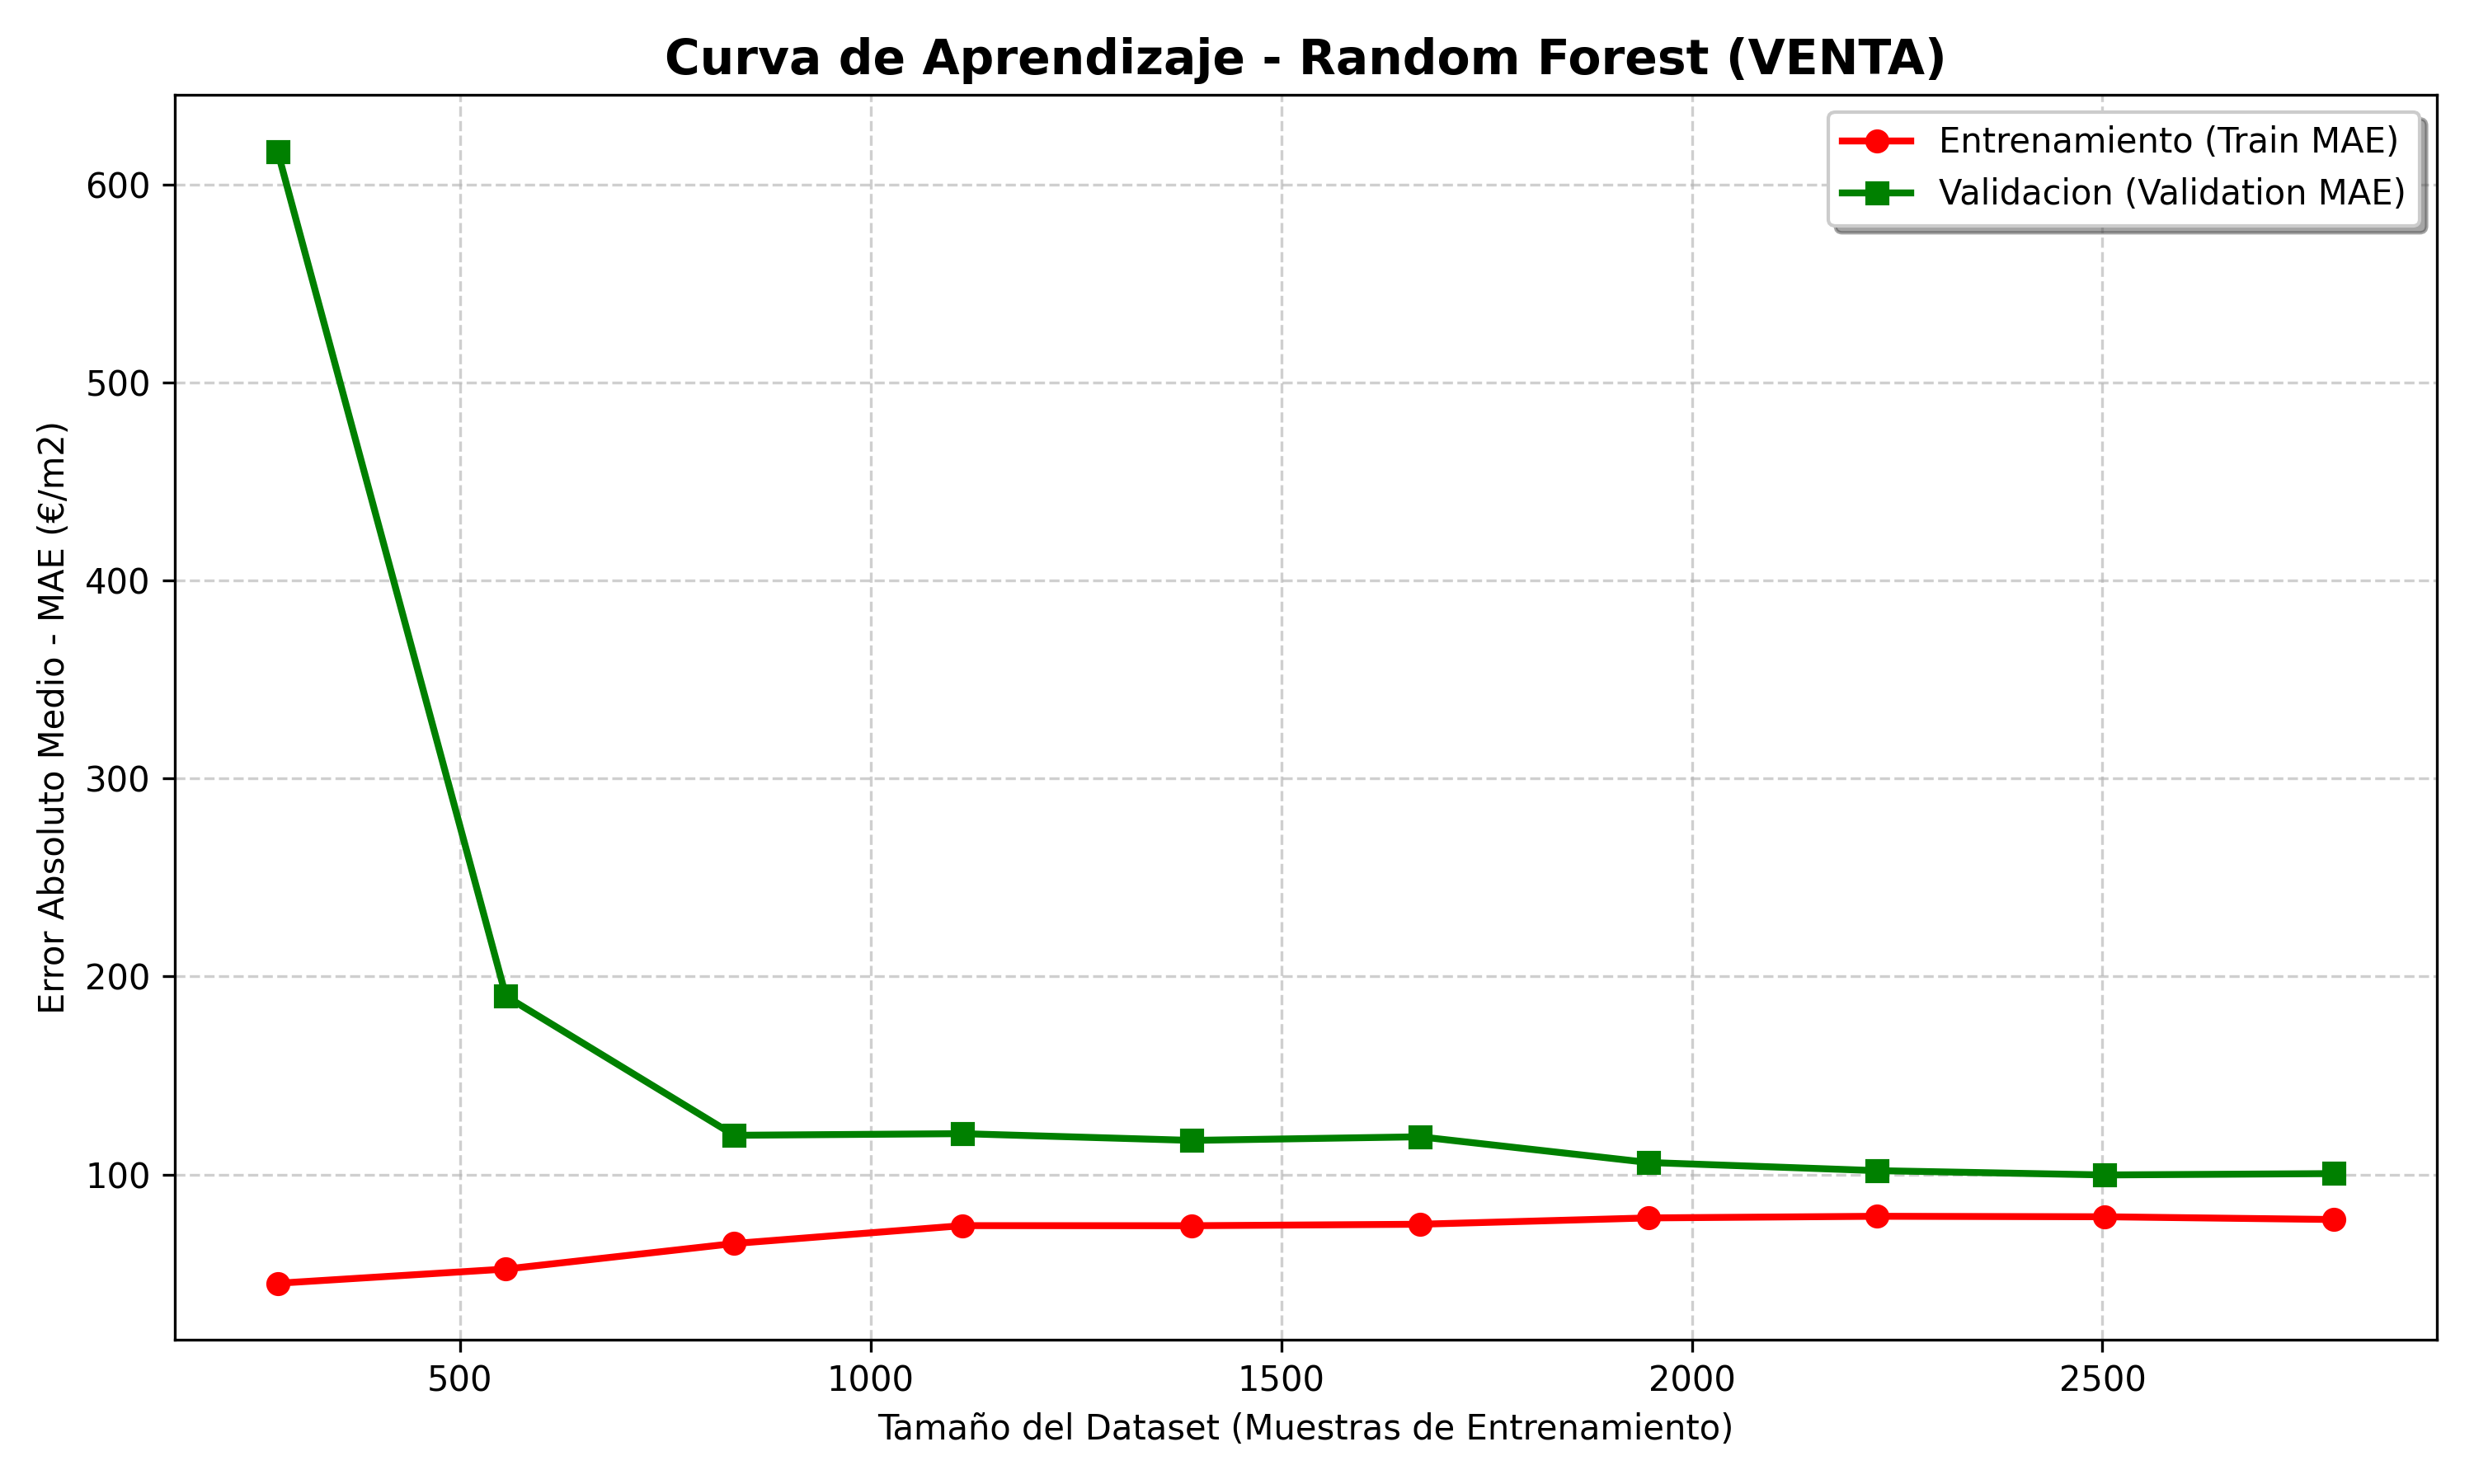
\includegraphics[width=0.40\linewidth]{img/phase2_learning_curve_random_forest_venta.png} & 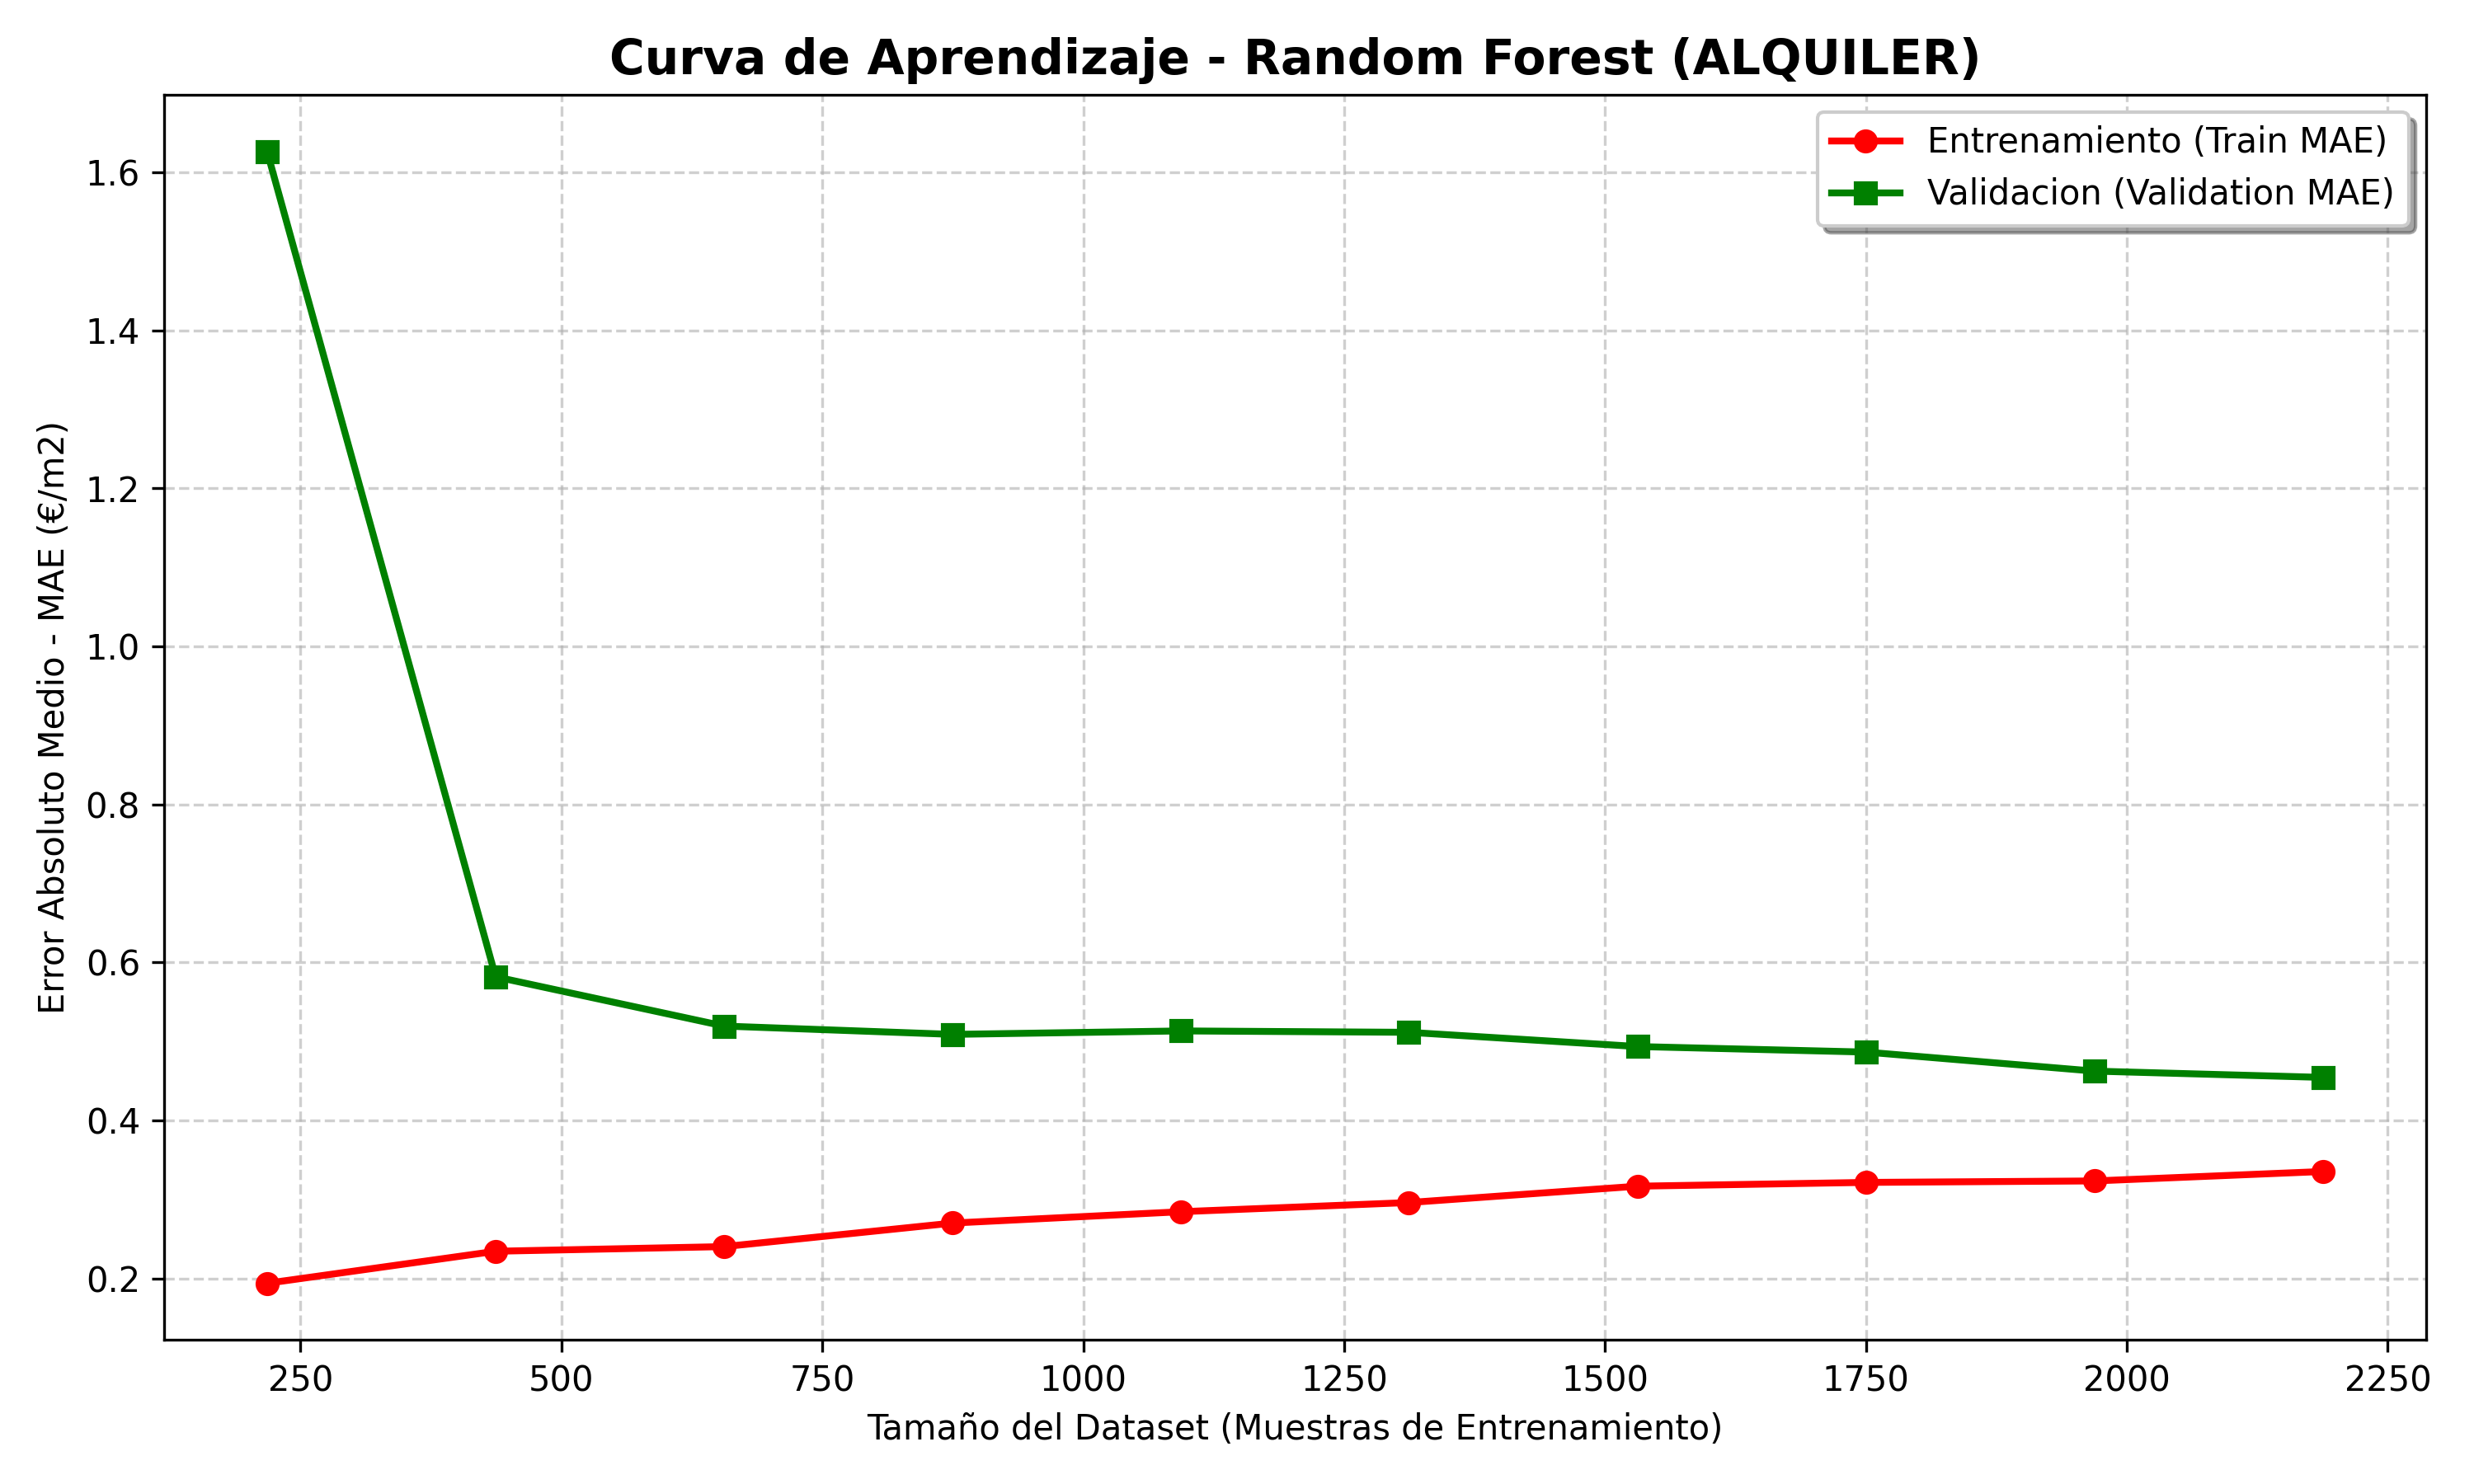
\includegraphics[width=0.40\linewidth]{img/phase2_learning_curve_random_forest_alquiler.png} \\
(a) Random Forest - Venta & (b) Random Forest - Alquiler \\
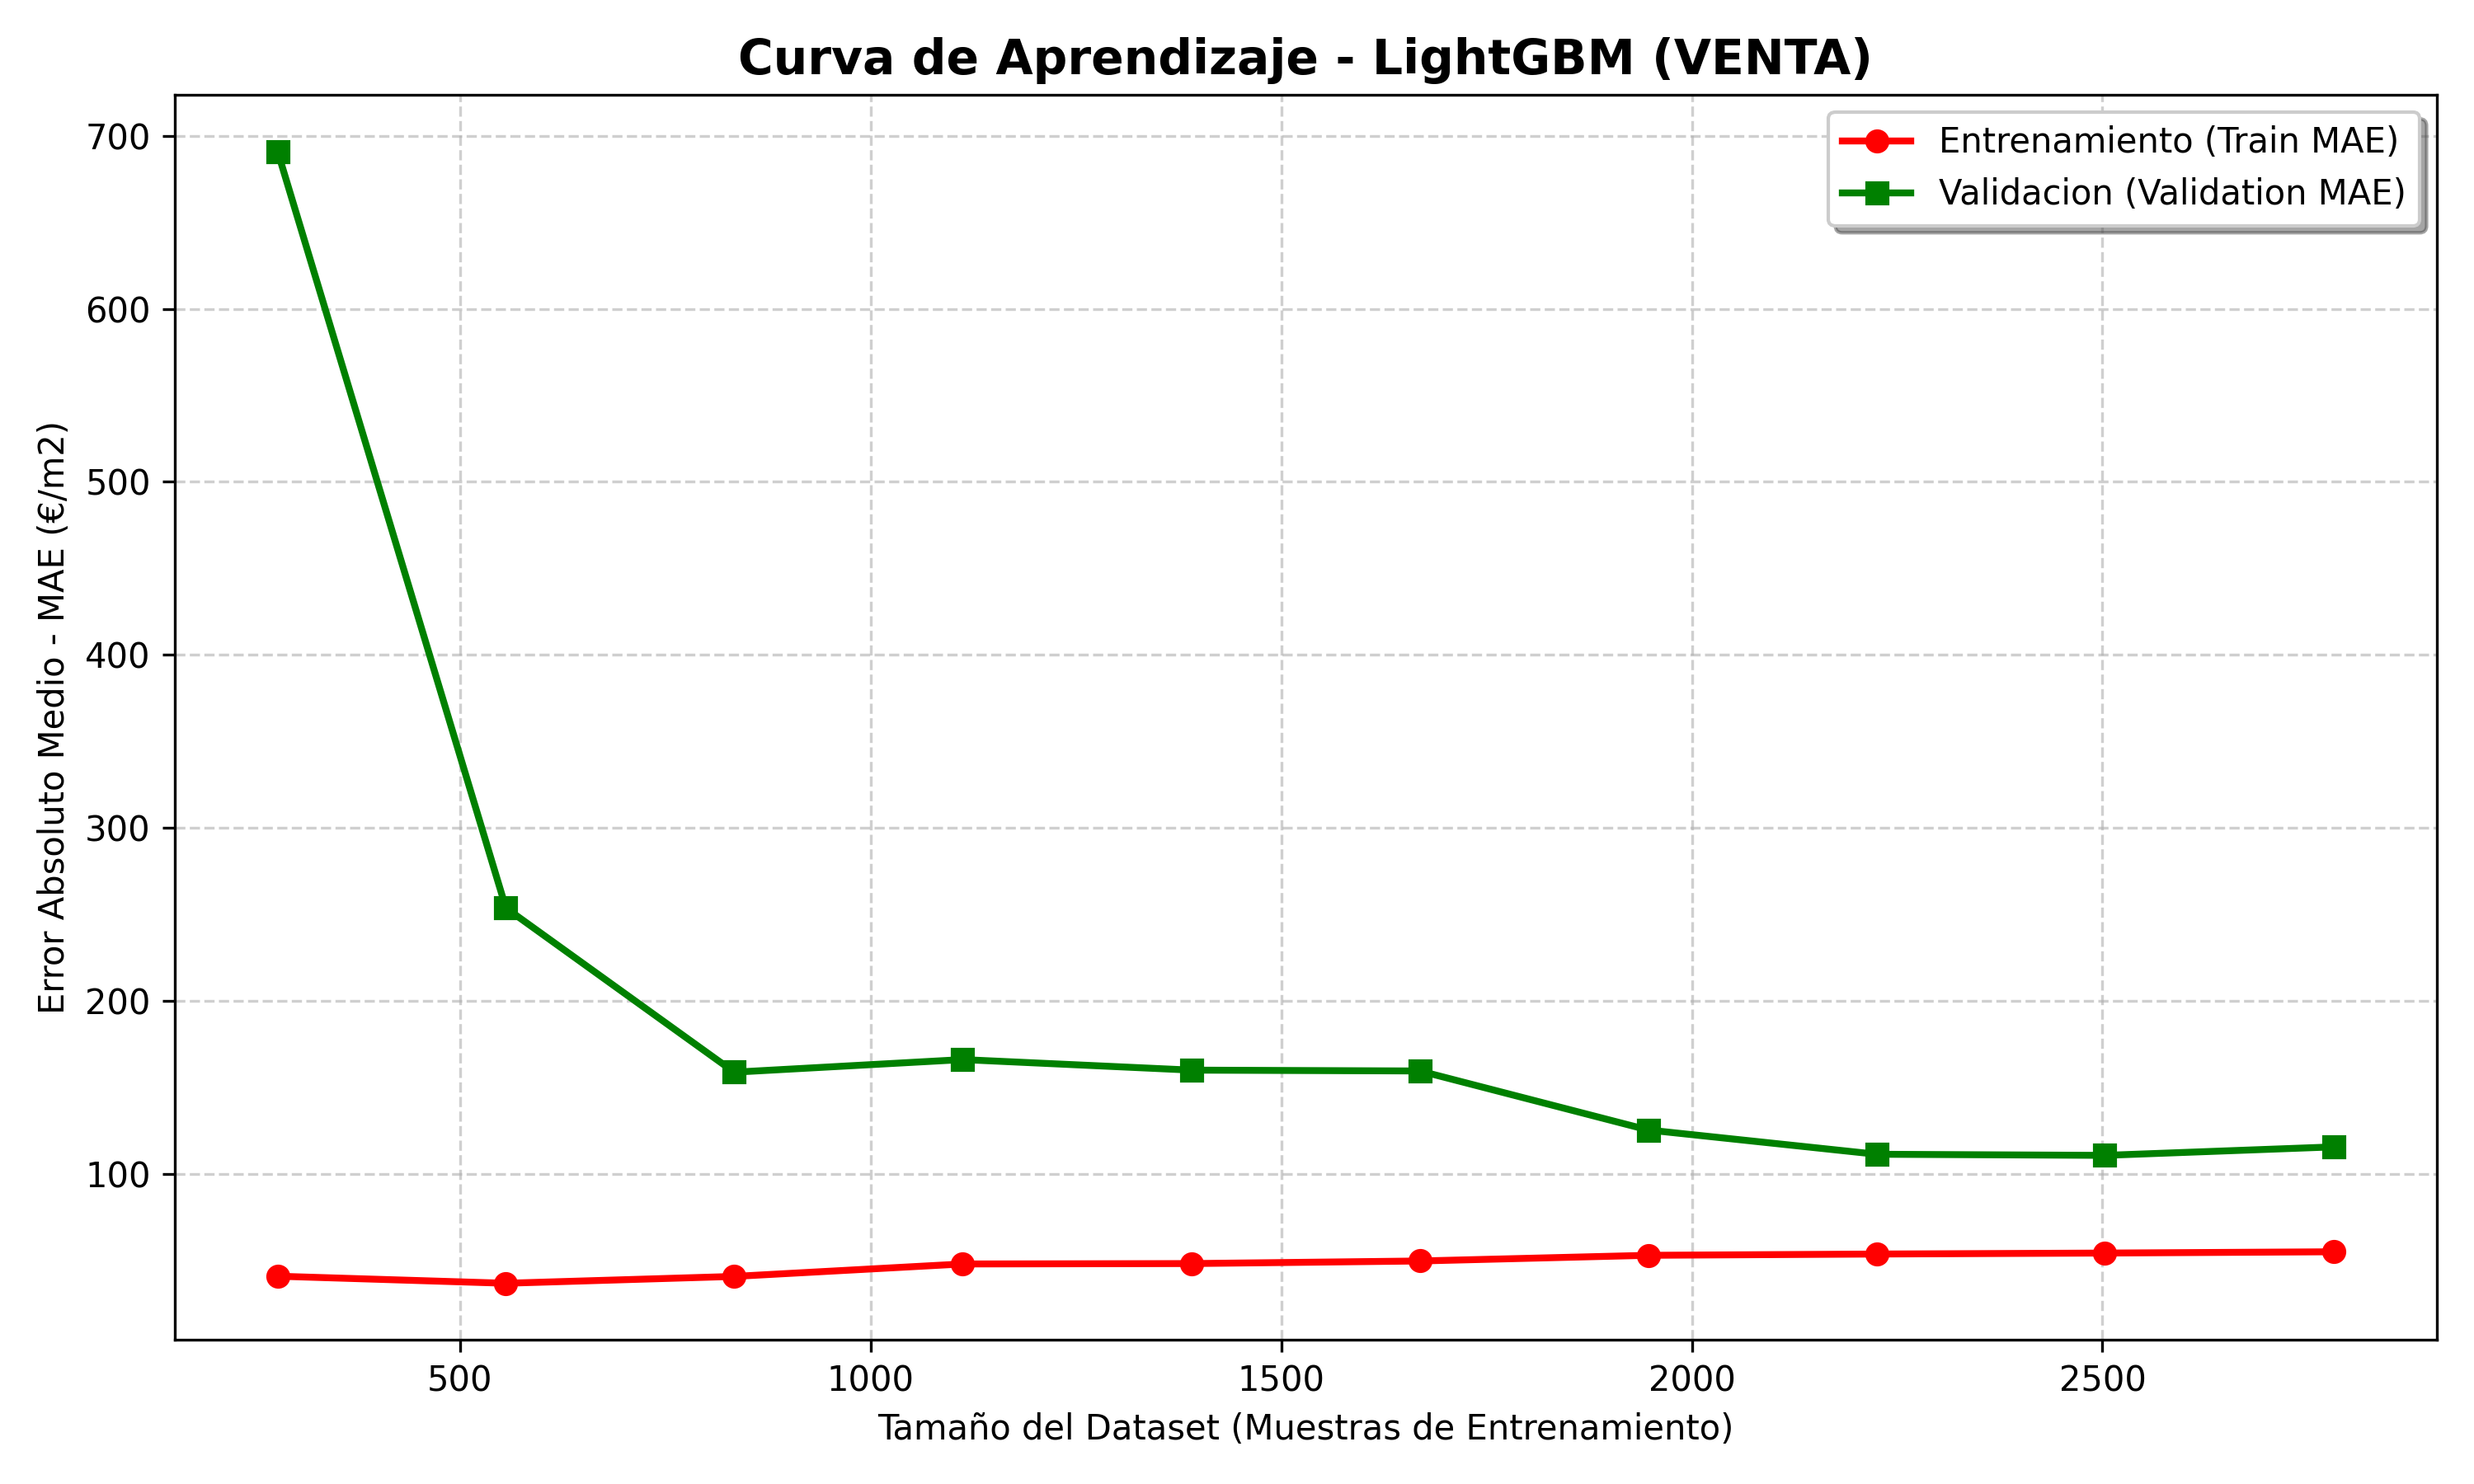
\includegraphics[width=0.40\linewidth]{img/phase2_learning_curve_lightgbm_venta.png} & 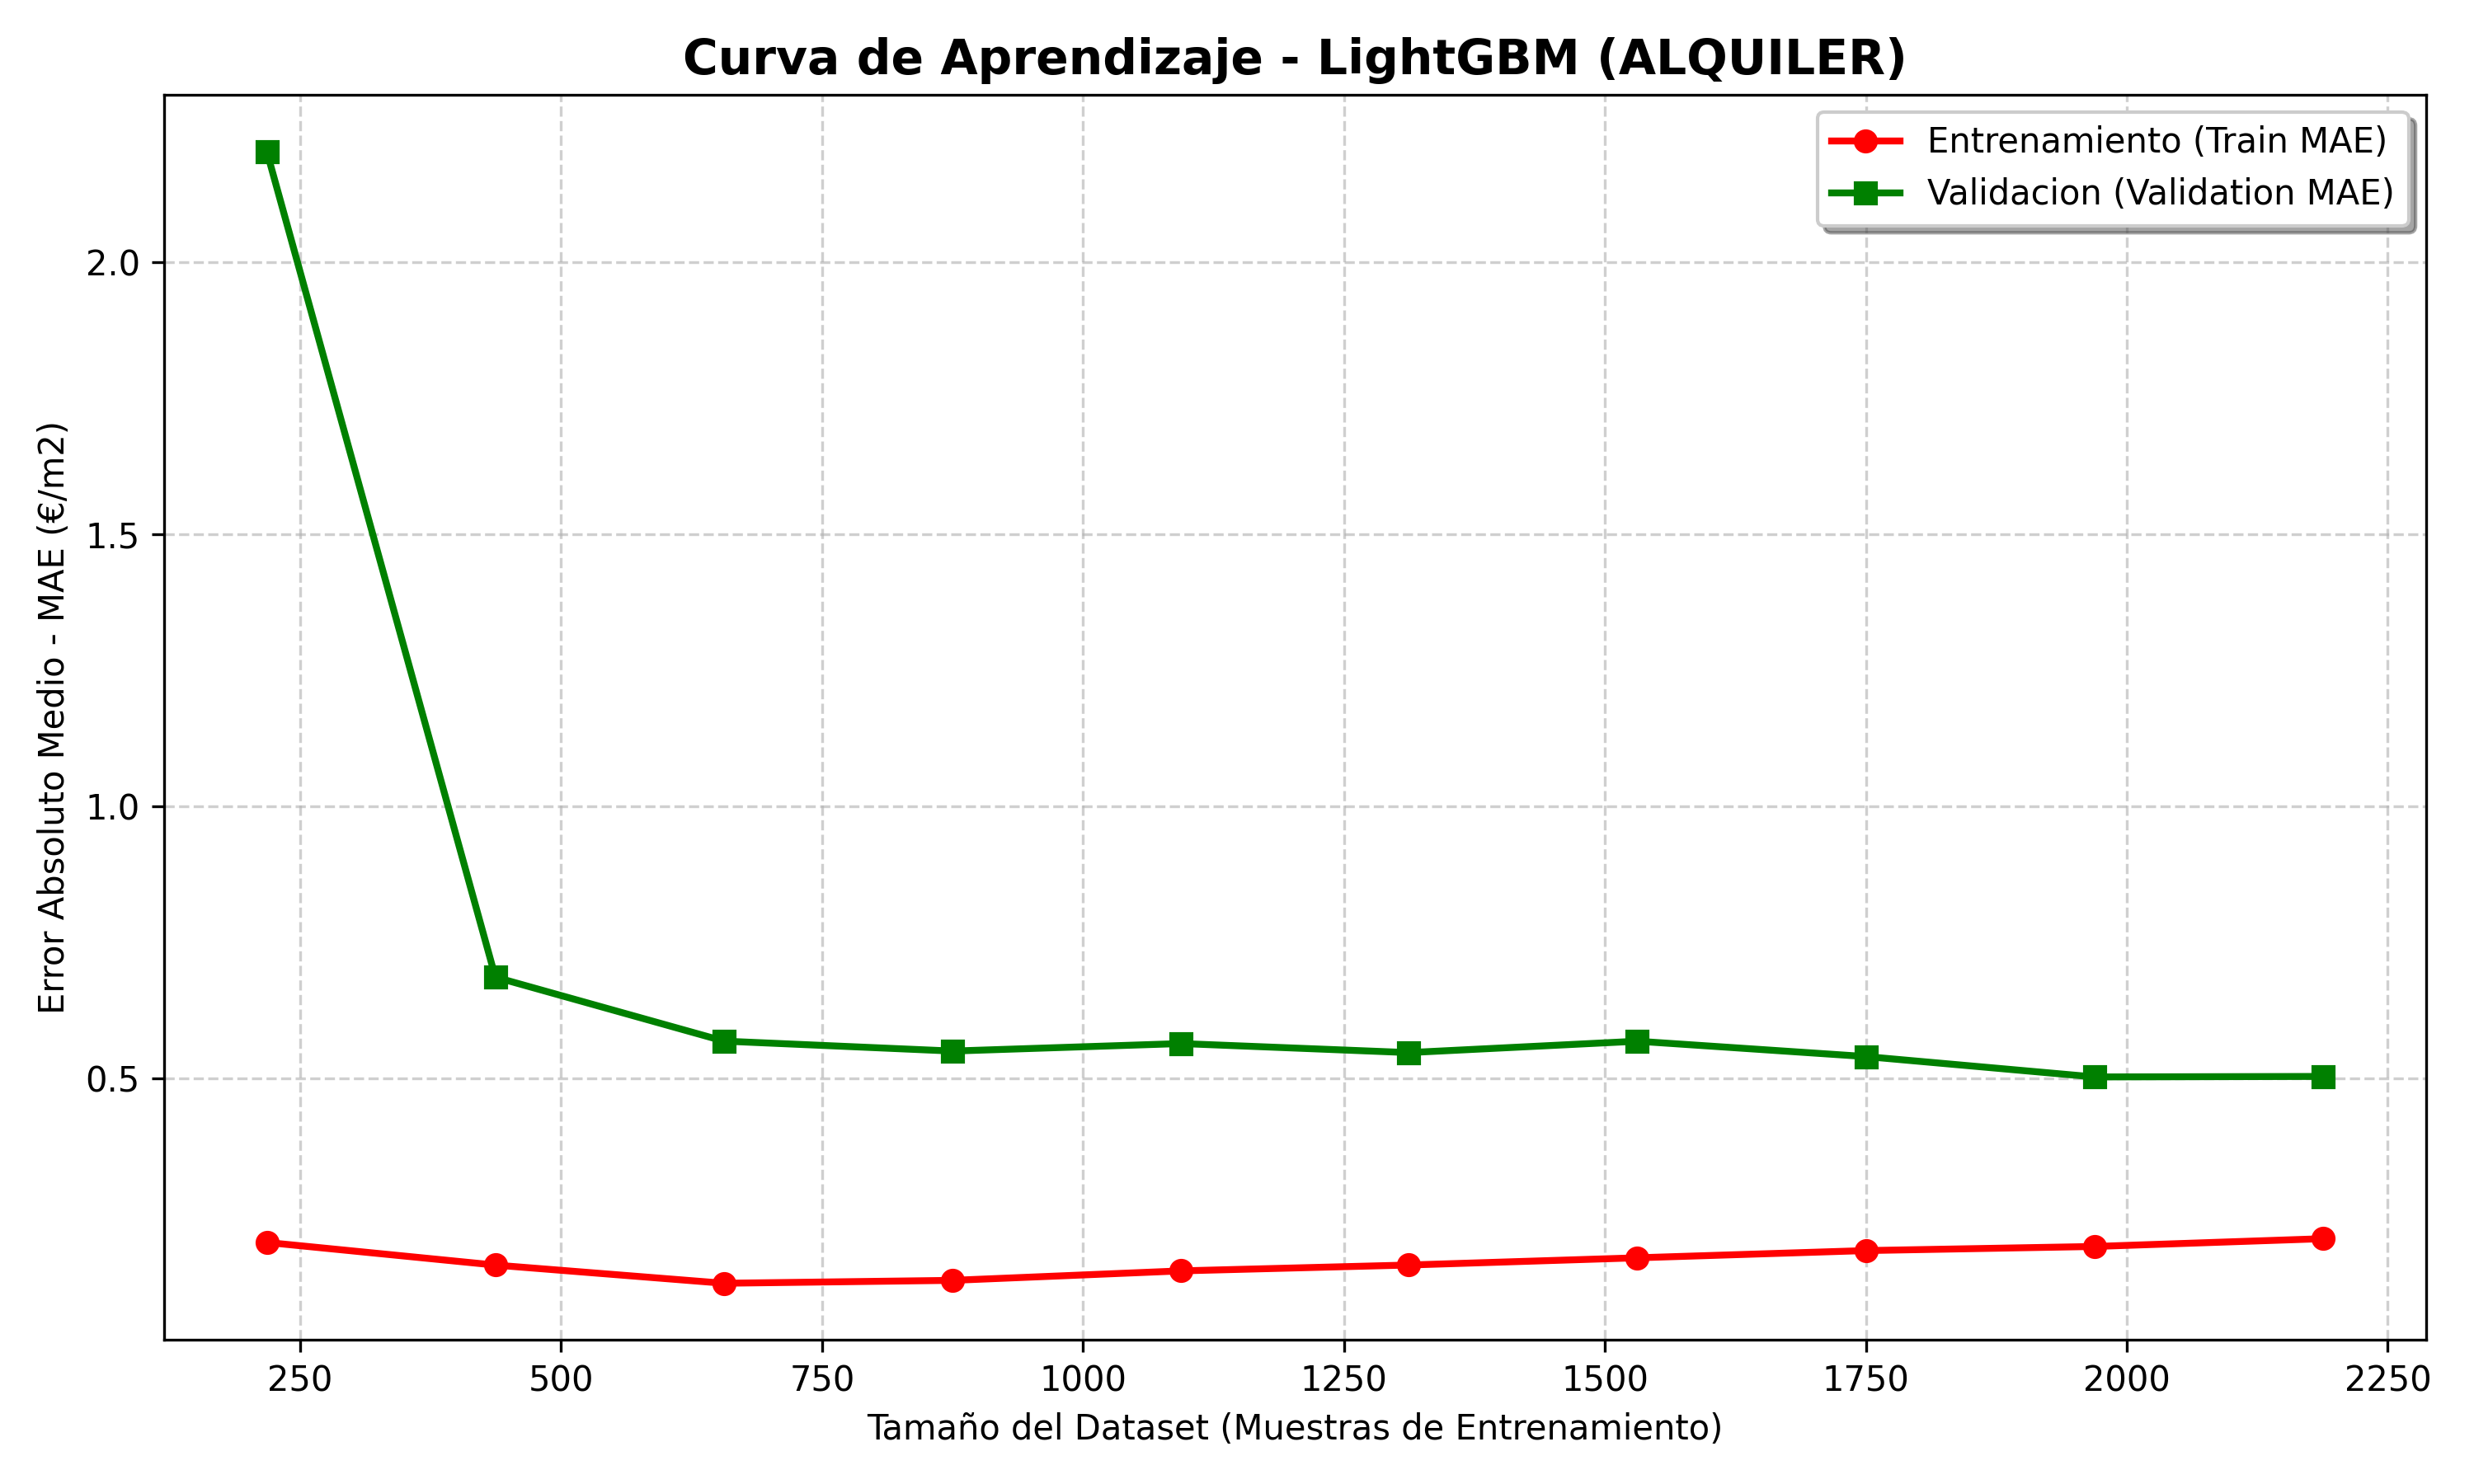
\includegraphics[width=0.40\linewidth]{img/phase2_learning_curve_lightgbm_alquiler.png} \\
(c) LightGBM - Venta & (d) LightGBM - Alquiler \\
\end{tabular}
\caption{Curvas de aprendizaje de Random Forest y LightGBM para los mercados de venta y alquiler en el modelado micro-local de barrio.}
\label{fig:learning_curves_phase2_rf_lgb}
\end{figure}

\begin{figure}[H]
\centering
\begin{tabular}{cc}
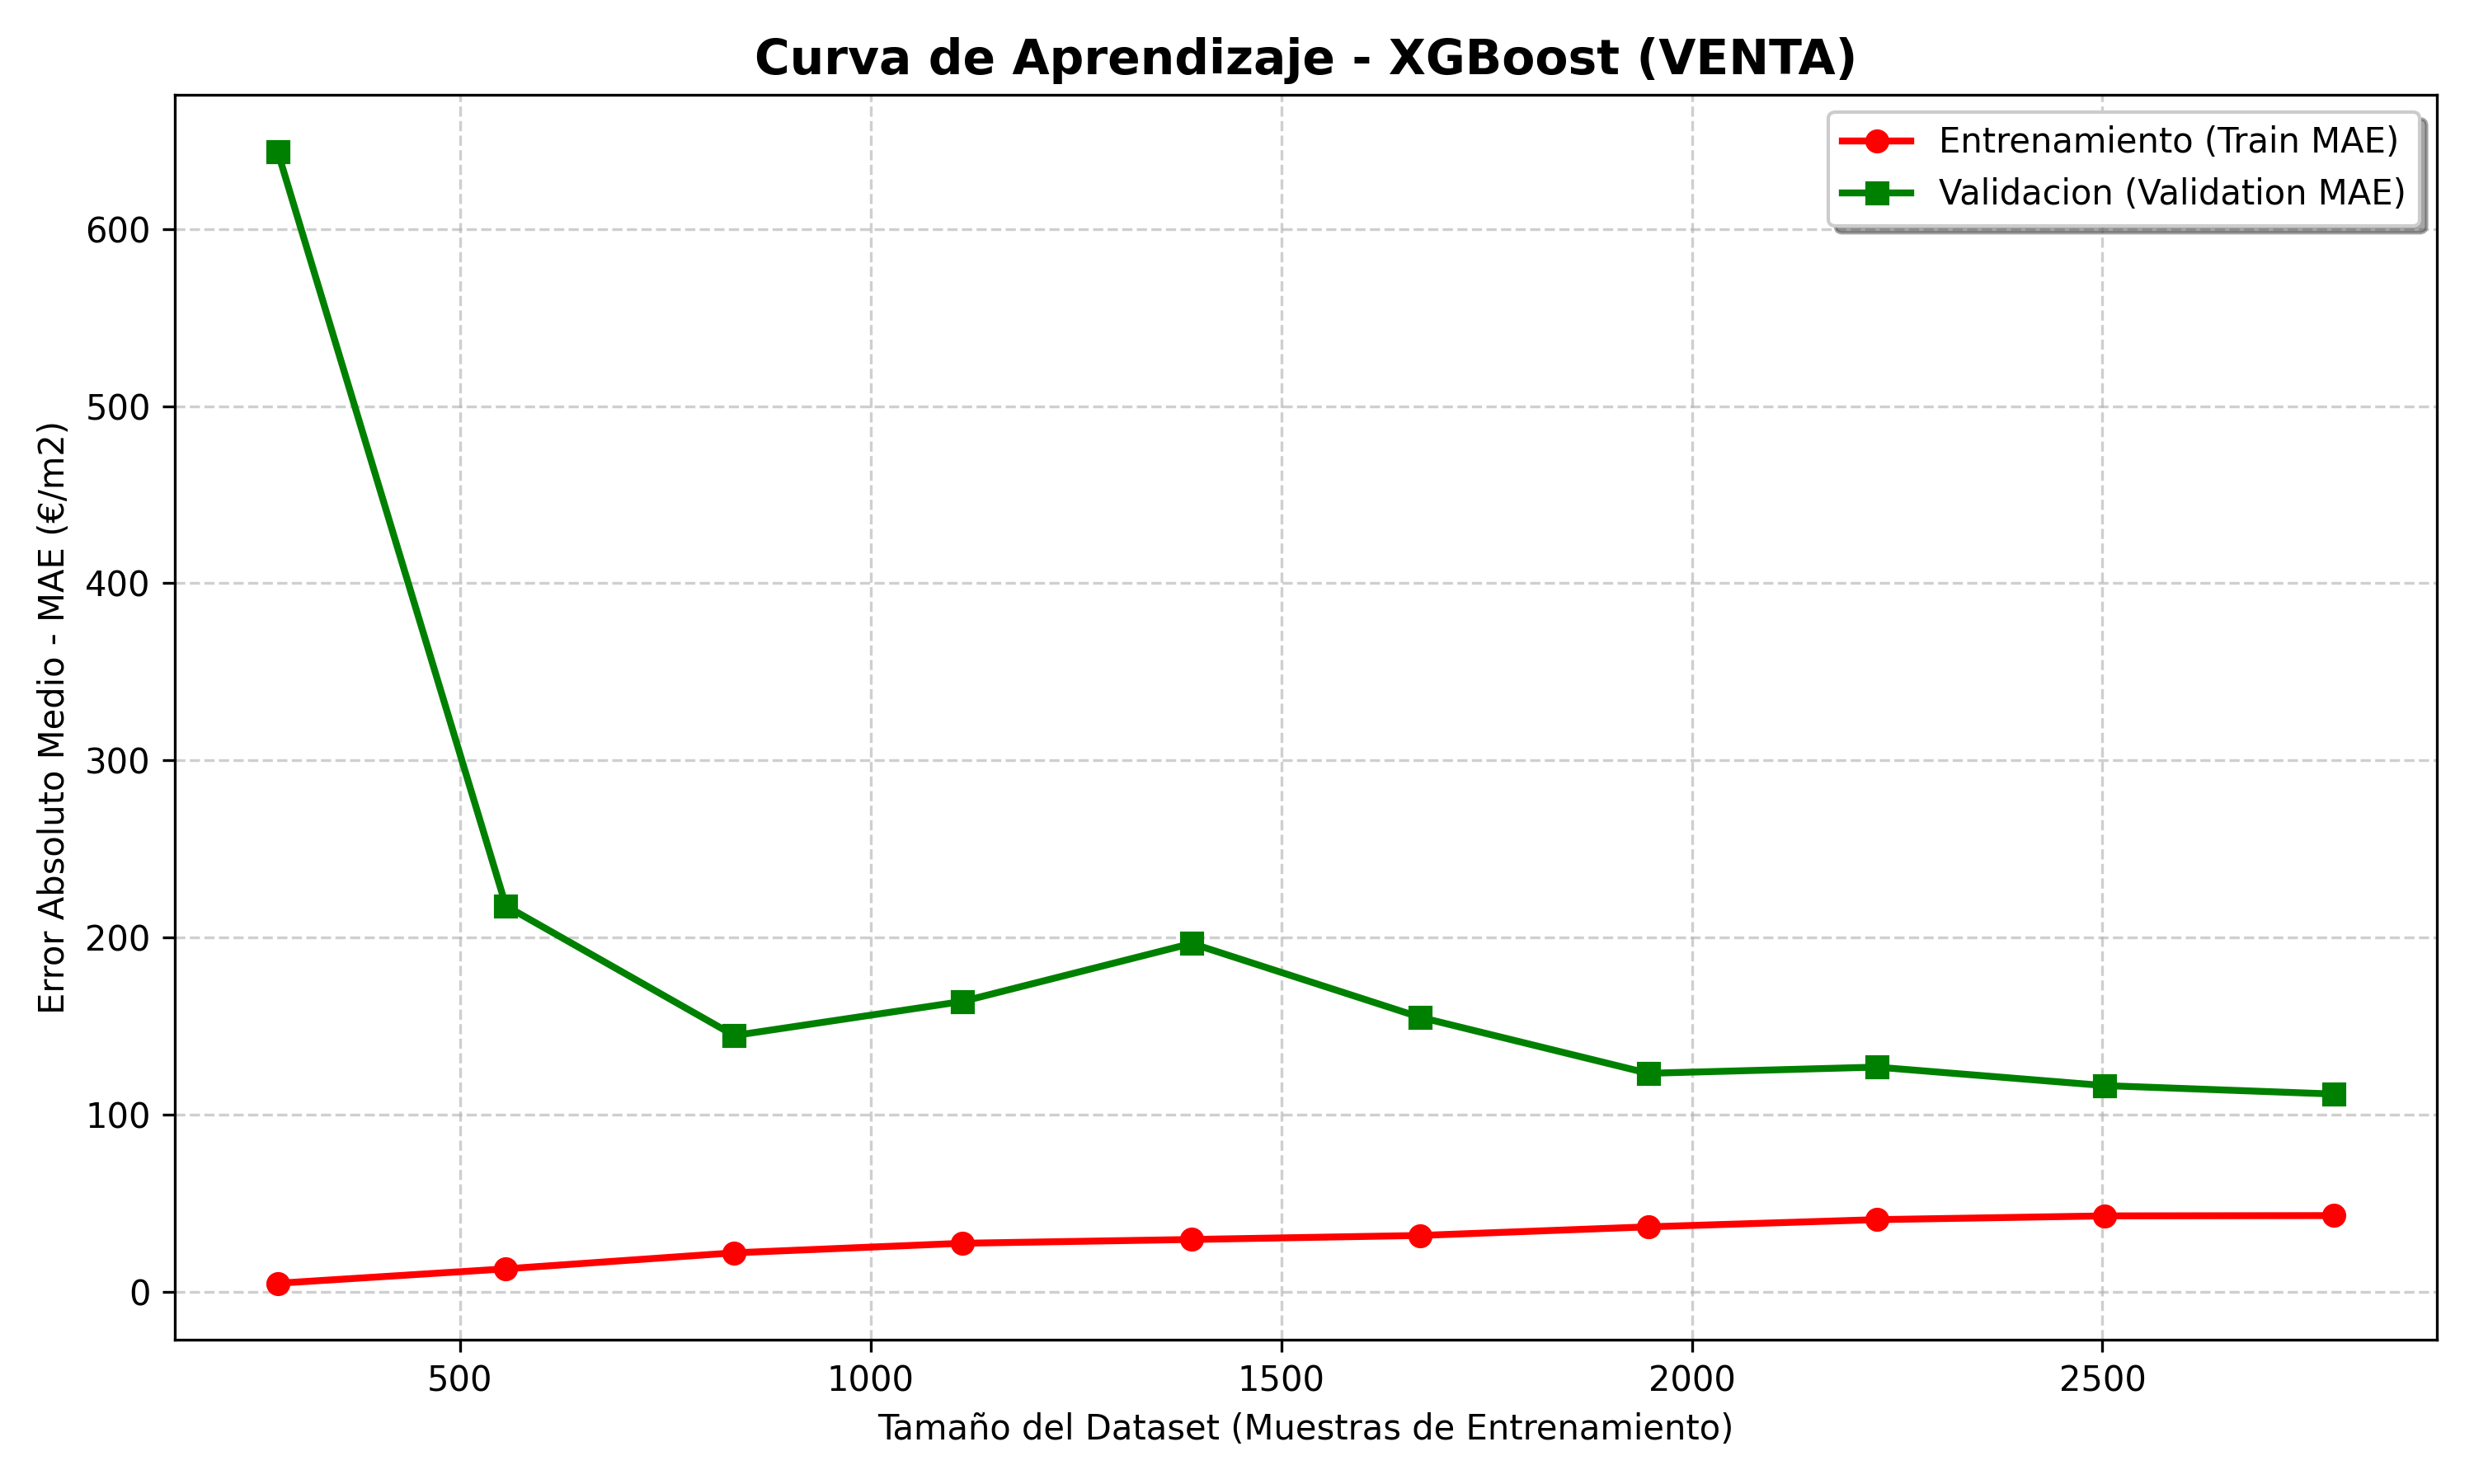
\includegraphics[width=0.40\linewidth]{img/phase2_learning_curve_xgboost_venta.png} & 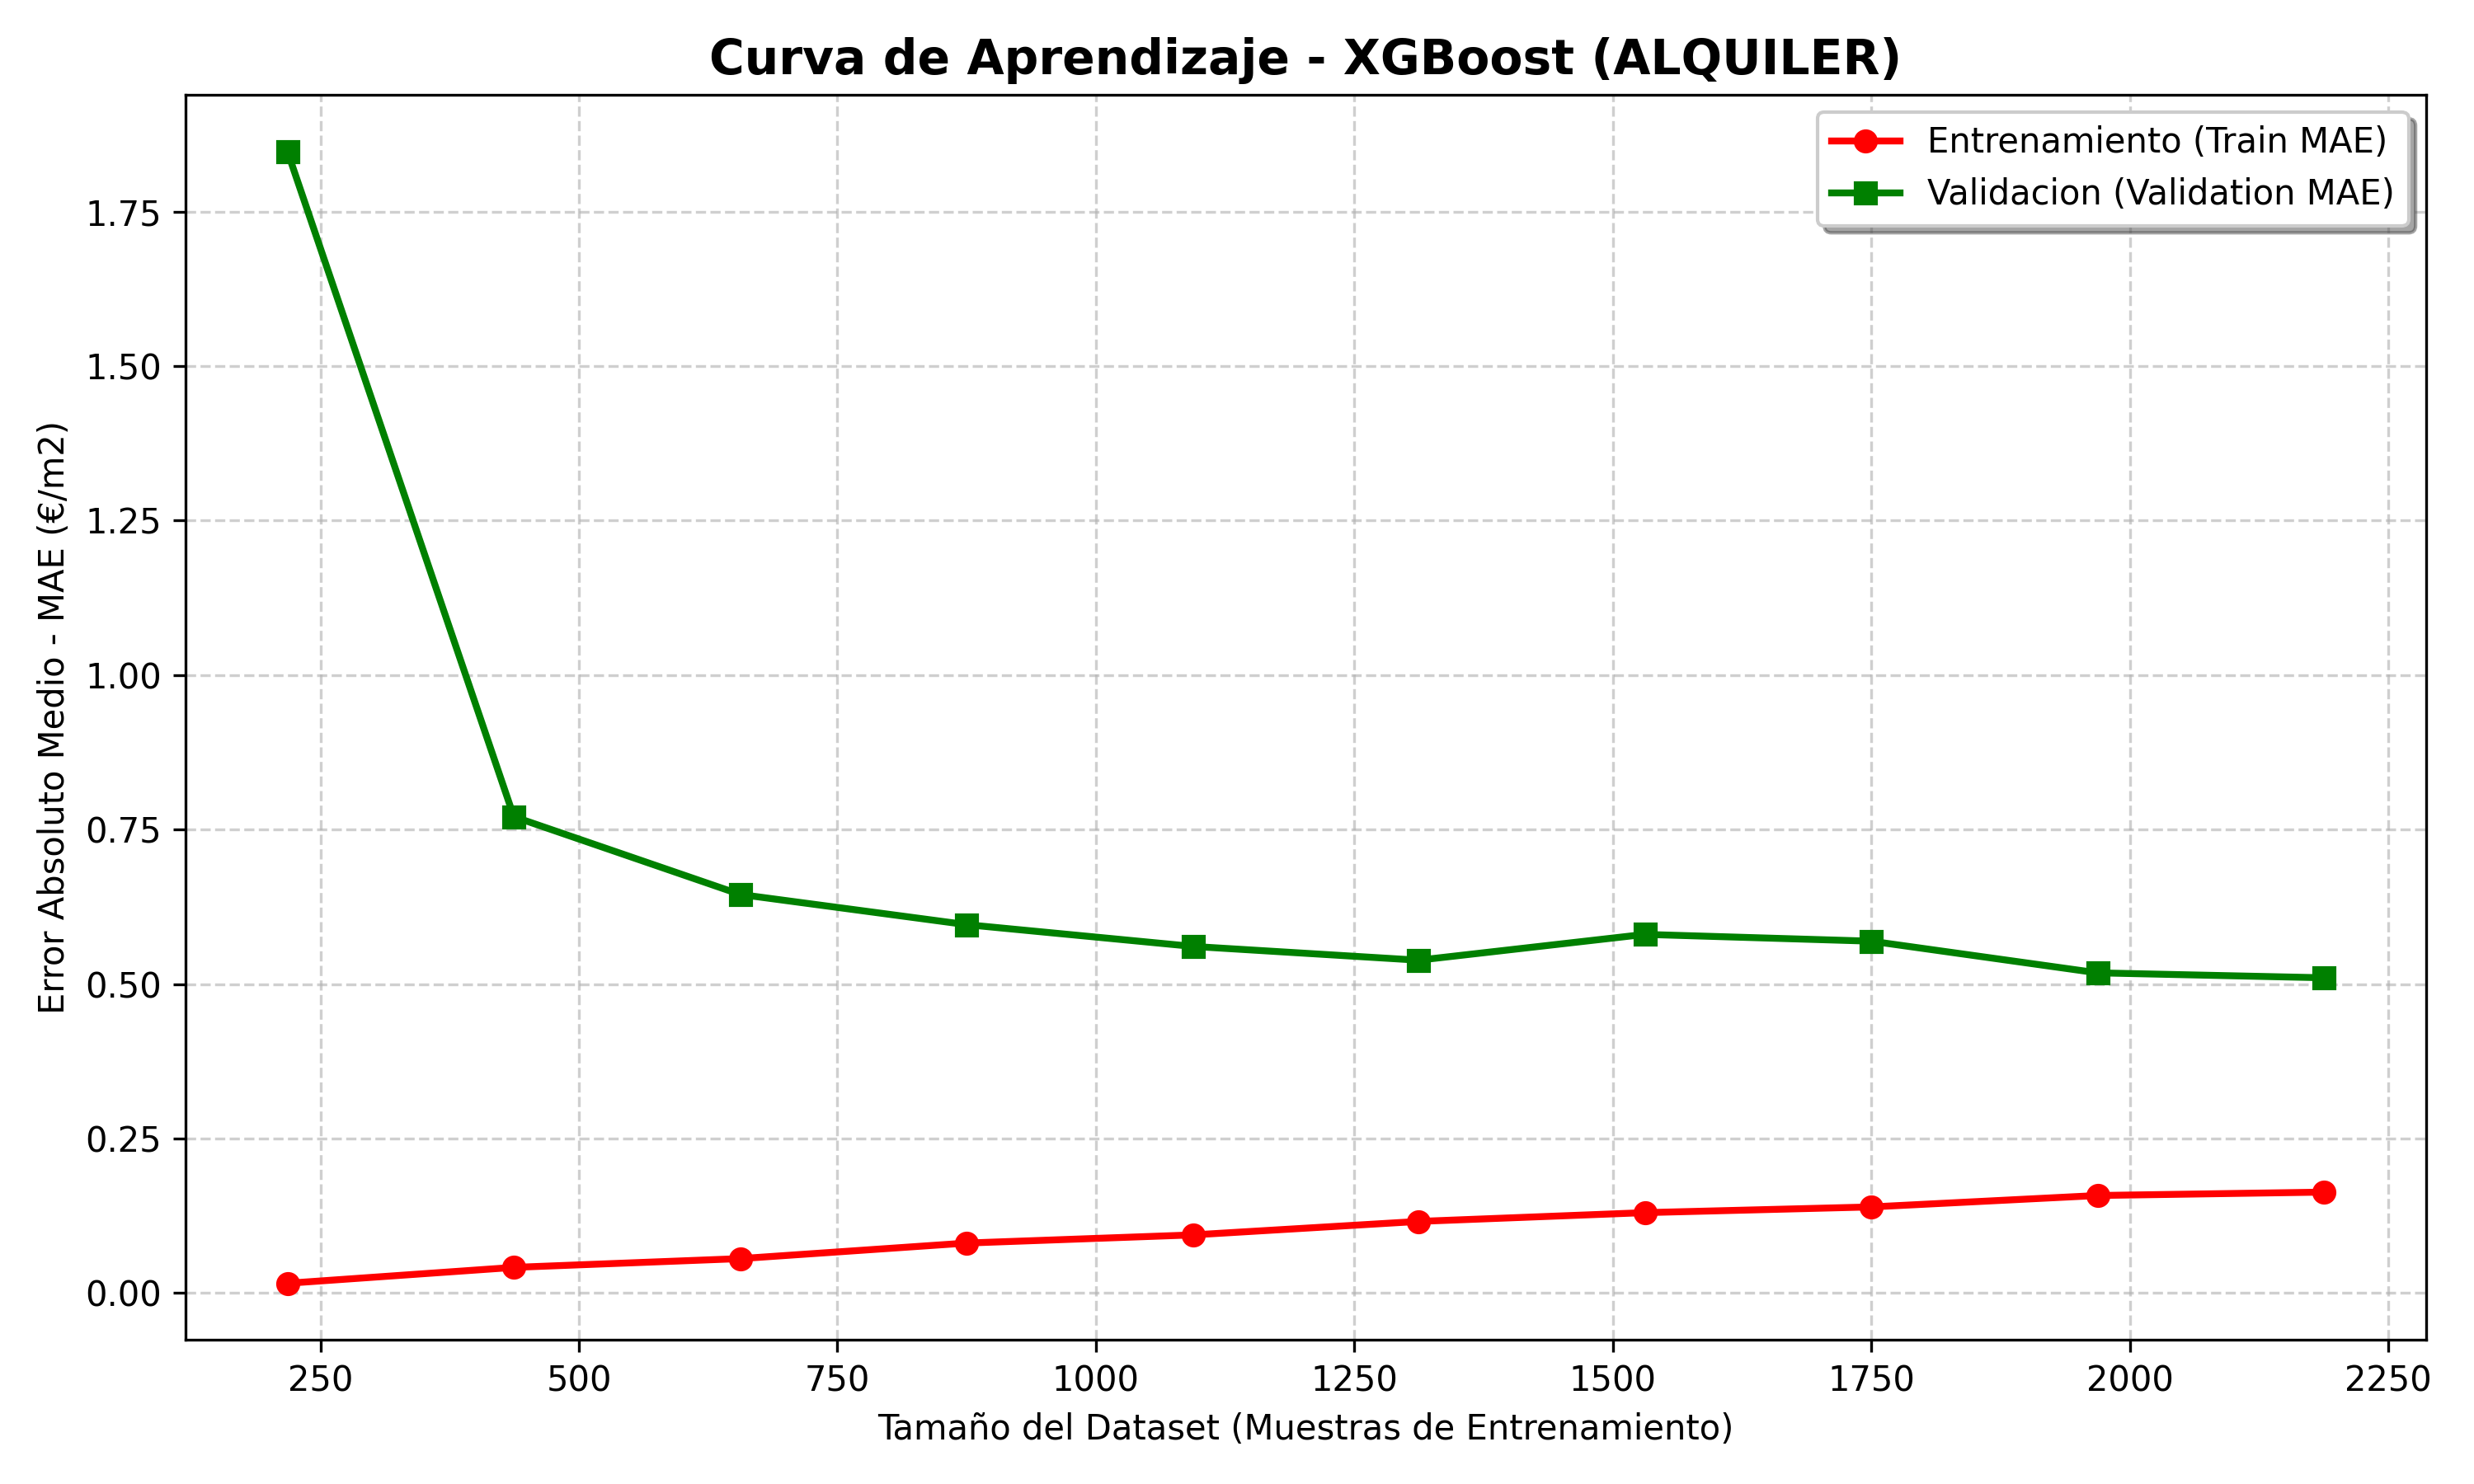
\includegraphics[width=0.40\linewidth]{img/phase2_learning_curve_xgboost_alquiler.png} \\
(a) XGBoost - Venta & (b) XGBoost - Alquiler \\
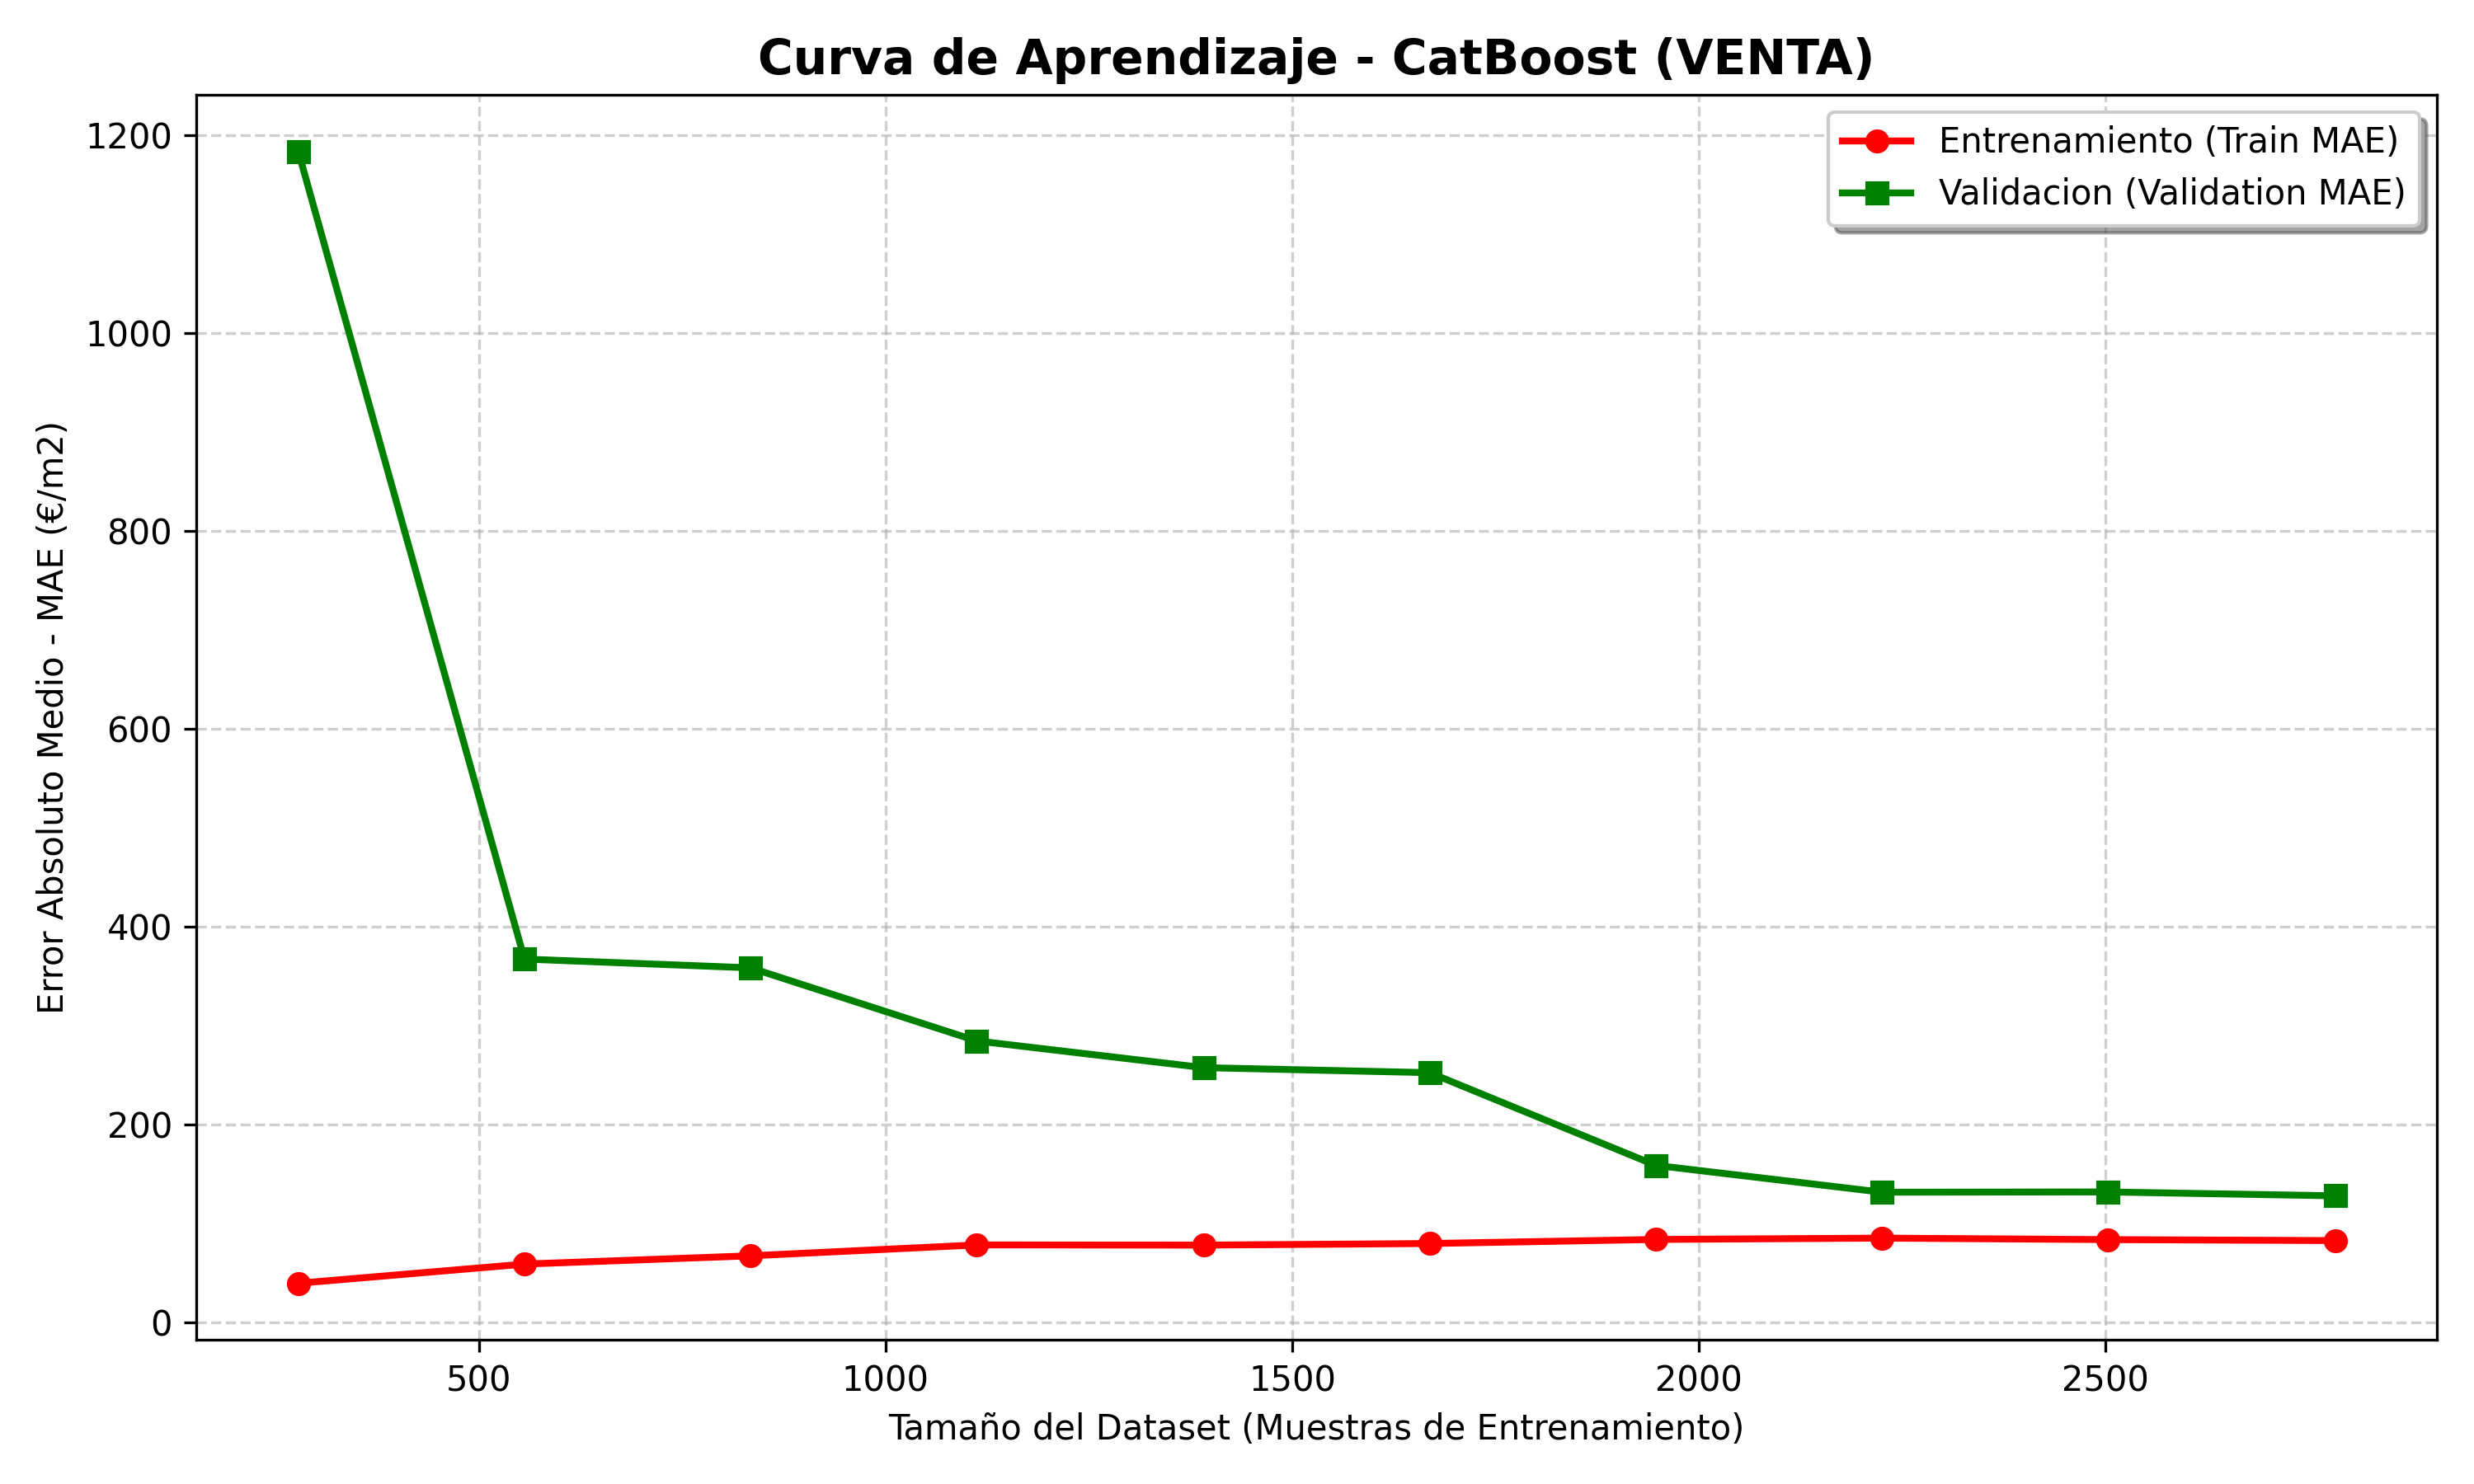
\includegraphics[width=0.40\linewidth]{img/phase2_learning_curve_catboost_venta.png} & 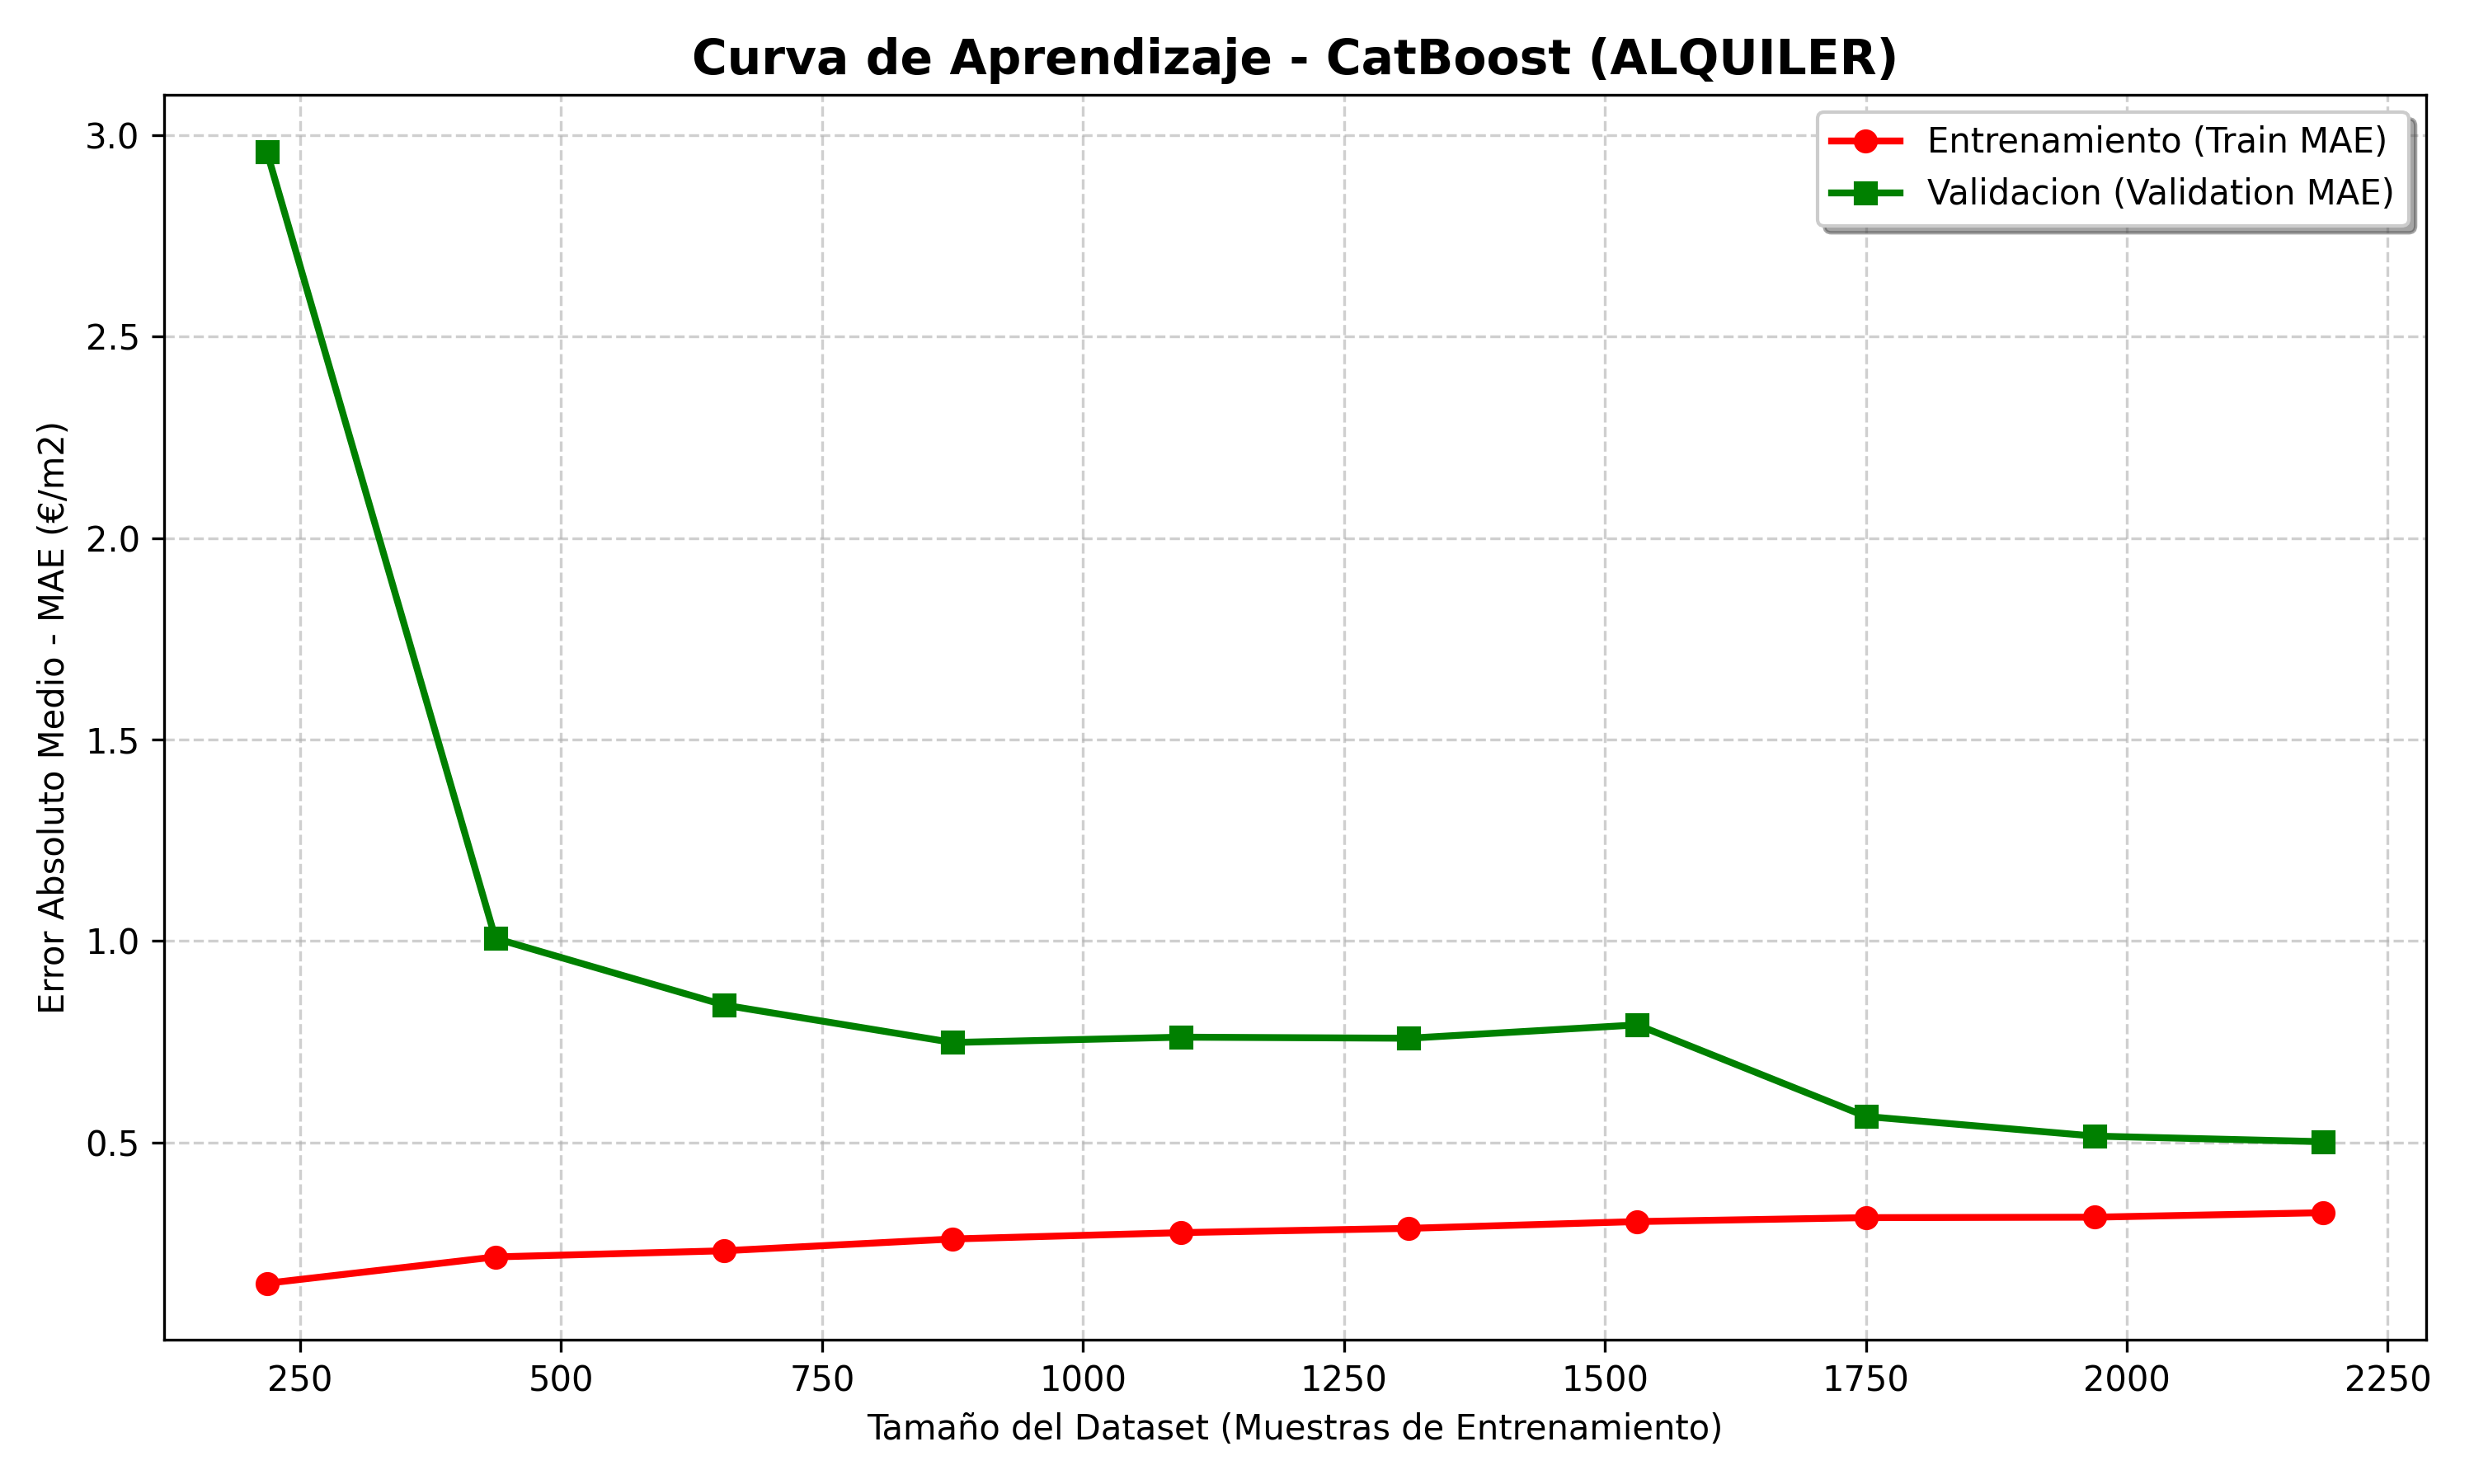
\includegraphics[width=0.40\linewidth]{img/phase2_learning_curve_catboost_alquiler.png} \\
(c) CatBoost - Venta & (d) CatBoost - Alquiler \\
\end{tabular}
\caption{Curvas de aprendizaje de XGBoost y CatBoost para los mercados de venta y alquiler en el modelado micro-local de barrio.}
\label{fig:learning_curves_phase2_xgb_cat}
\end{figure}

Las curvas de aprendizaje a nivel de barrio (Figura~\ref{fig:learning_curves_phase2_rf_lgb} y Figura~\ref{fig:learning_curves_phase2_xgb_cat}) muestran un patrón de convergencia de error a medida que el tamaño del dataset se aproxima a su capacidad máxima. En los modelos de gradiente boosting, XGBoost y LightGBM exhiben una convergencia muy limpia, donde la curva de validación (línea verde) desciende suavemente hasta estabilizarse muy cerca de la de entrenamiento (línea roja), lo que descarta problemas de sobreajuste. En el caso de CatBoost, la convergencia es igualmente estable aunque con un descenso ligeramente más atenuado en las etapas iniciales de datos. Por su parte, Random Forest muestra una separación típica debido a su naturaleza de ensamble por embolsado (bagging), el error de entrenamiento se mantiene cercano a cero mientras que la curva de validación se estabiliza rápidamente en valores bajos a partir de un volumen medio de muestras, lo que confirma la solidez general del aprendizaje en este nivel micro-local.

\subsubsection{Alineación de Escalas Territoriales a Nivel de Distrito}
Finalmente, la tercera etapa consistió en entrenar y evaluar los modelos en una escala territorial agregada homogénea de distrito (\texttt{id\_barrio == -1}). Al no estar expuestos a la dispersión de precios micro-local de los barrios, los modelos sobre distritos arrojaron errores globales muy reducidos (XGBoost alcanzó en venta un MAE de \textbf{74,64 €/m\textsuperscript{2}} y en alquiler de \textbf{0,293 €/m\textsuperscript{2}}), tal como se expone en la Tabla~\ref{tab:phase3_distrito_venta} y la Tabla~\ref{tab:phase3_distrito_alquiler}. 

Como se detalló anteriormente, esta aparente mejora es en realidad un artefacto estadístico provocado por el efecto suavizado de la agregación espacial, la cual elimina el ruido y los picos del mercado inmobiliario y diluye los extremos en un único registro ponderado mensual. En consecuencia, el modelado distrital colapsa en validación out-of-sample en zonas premium locales, lo que demuestra que la granularidad de barrio es indispensable para el desarrollo de un motor predictivo fiable.

\begin{table}[H]
\centering
\caption{Matriz de rendimiento comparativa: Alineación de escalas a nivel agregado de distrito con retardos temporales - Mercado de Venta (€/m\textsuperscript{2})}
\label{tab:phase3_distrito_venta}
\resizebox{\textwidth}{!}{%
\begin{tabular}{|l|c|c|c|c|c|c|c|c|c|c|c|}
\hline
\textbf{Algoritmo} & \textbf{MAE} & \textbf{RMSE} & \textbf{R\textsuperscript{2}} & \textbf{MAPE} & \textbf{Sesgo} & \textbf{MAE} & \textbf{R\textsuperscript{2}} & \textbf{MAE} & \textbf{R\textsuperscript{2}} & \textbf{T. Train} & \textbf{T. Pred} \\
 & \textbf{Global} & \textbf{Global} & \textbf{Global} & \textbf{Global (\%)} & \textbf{Global} & \textbf{Salamanca} & \textbf{Salamanca} & \textbf{C. Lineal} & \textbf{C. Lineal} & \textbf{(s)} & \textbf{(s)} \\
\hline
\textbf{Random Forest} & 85,69 & 126,78 & 0,9959 & 1,38\% & 35,23 & 162,88 & -3,4947 & 242,16 & -6,9854 & 0,460 & 0,044 \\
\textbf{CatBoost} & 169,85 & 245,34 & 0,9846 & 3,01\% & -72,14 & \textbf{44,80} & \textbf{0,5218} & 766,58 & -68,4342 & 1,102 & 0,003 \\
\textbf{XGBoost} & \textbf{74,64} & \textbf{100,20} & \textbf{0,9974} & \textbf{1,36\%} & \textbf{-1,22} & 92,66 & -0,3538 & \textbf{239,99} & \textbf{-6,7082} & 0,550 & 0,005 \\
\textbf{LightGBM} & 143,88 & 235,94 & 0,9858 & 2,24\% & 24,20 & 252,89 & -8,9002 & 638,88 & -47,2667 & \textbf{0,190} & \textbf{0,002} \\
\hline
\end{tabular}%
}
\end{table}

\begin{table}[H]
\centering
\caption{Matriz de rendimiento comparativa: Alineación de escalas a nivel agregado de distrito con retardos temporales - Mercado de Alquiler (€/m\textsuperscript{2})}
\label{tab:phase3_distrito_alquiler}
\resizebox{\textwidth}{!}{%
\begin{tabular}{|l|c|c|c|c|c|c|c|c|c|c|c|}
\hline
\textbf{Algoritmo} & \textbf{MAE} & \textbf{RMSE} & \textbf{R\textsuperscript{2}} & \textbf{MAPE} & \textbf{Sesgo} & \textbf{MAE} & \textbf{R\textsuperscript{2}} & \textbf{MAE} & \textbf{R\textsuperscript{2}} & \textbf{T. Train} & \textbf{T. Pred} \\
 & \textbf{Global} & \textbf{Global} & \textbf{Global} & \textbf{Global (\%)} & \textbf{Global} & \textbf{Salamanca} & \textbf{Salamanca} & \textbf{C. Lineal} & \textbf{C. Lineal} & \textbf{(s)} & \textbf{(s)} \\
\hline
\textbf{Random Forest} & \textbf{0,285} & \textbf{0,363} & \textbf{0,9897} & \textbf{1,44\%} & \textbf{-0,038} & 0,212 & -2,1167 & \textbf{0,529} & -10,0005 & 0,464 & 0,043 \\
\textbf{CatBoost} & 0,530 & 0,739 & 0,9572 & 2,45\% & -0,259 & 1,498 & -96,4203 & 1,969 & -138,4821 & 0,983 & 0,003 \\
\textbf{XGBoost} & 0,293 & 0,391 & 0,9880 & 1,50\% & -0,086 & \textbf{0,199} & \textbf{-1,4167} & 0,562 & \textbf{-11,2224} & 0,591 & 0,006 \\
\textbf{LightGBM} & 0,395 & 0,541 & 0,9771 & 1,87\% & -0,139 & 1,012 & -43,3445 & 1,461 & -76,0750 & \textbf{0,139} & \textbf{0,002} \\
\hline
\end{tabular}%
}
\end{table}

Al contrastar de forma analítica los resultados del modelado agregado a nivel de distrito expuestos en la Tabla~\ref{tab:phase3_distrito_venta} y la Tabla~\ref{tab:phase3_distrito_alquiler} frente al escenario previo de barrio, se revelan comportamientos divergentes según la arquitectura algorítmica utilizada. En el mercado de venta, los modelos de Random Forest y XGBoost reducen sustancialmente sus errores predictivos en esta escala agregada; XGBoost alcanza un MAE global mínimo de 74,64 \text{€/m\textsuperscript{2}} (frente a 111,67 \text{€/m\textsuperscript{2}} a nivel de barrio) y Random Forest un MAE de 85,69 \text{€/m\textsuperscript{2}} (frente a 100,50 \text{€/m\textsuperscript{2}}). Por el contrario, los modelos CatBoost (169,85 \text{€/m\textsuperscript{2}}) y LightGBM (143,88 \text{€/m\textsuperscript{2}}) incrementan su MAE, RMSE y reducen su R\textsuperscript{2} en comparación con la escala local de barrio. Es notable destacar que los sesgos predictivos globales se reducen al mínimo absoluto en esta escala, con XGBoost registrando apenas -1,22 \text{€/m\textsuperscript{2}}. Sin embargo, el comportamiento local en Salamanca y Ciudad Lineal muestra una gran dispersión residual. En lo que respecta al mercado de alquiler, se reproduce un comportamiento similar donde Random Forest (MAE de 0,285 \text{€/m\textsuperscript{2}}), XGBoost (0,293 \text{€/m\textsuperscript{2}}) y LightGBM (0,395 \text{€/m\textsuperscript{2}}) mejoran considerablemente frente a la granularidad de barrio, mientras que CatBoost se mantiene relativamente indiferente (con un MAE de 0,530 \text{€/m\textsuperscript{2}}).

\begin{figure}[H]
\centering
\begin{tabular}{cc}
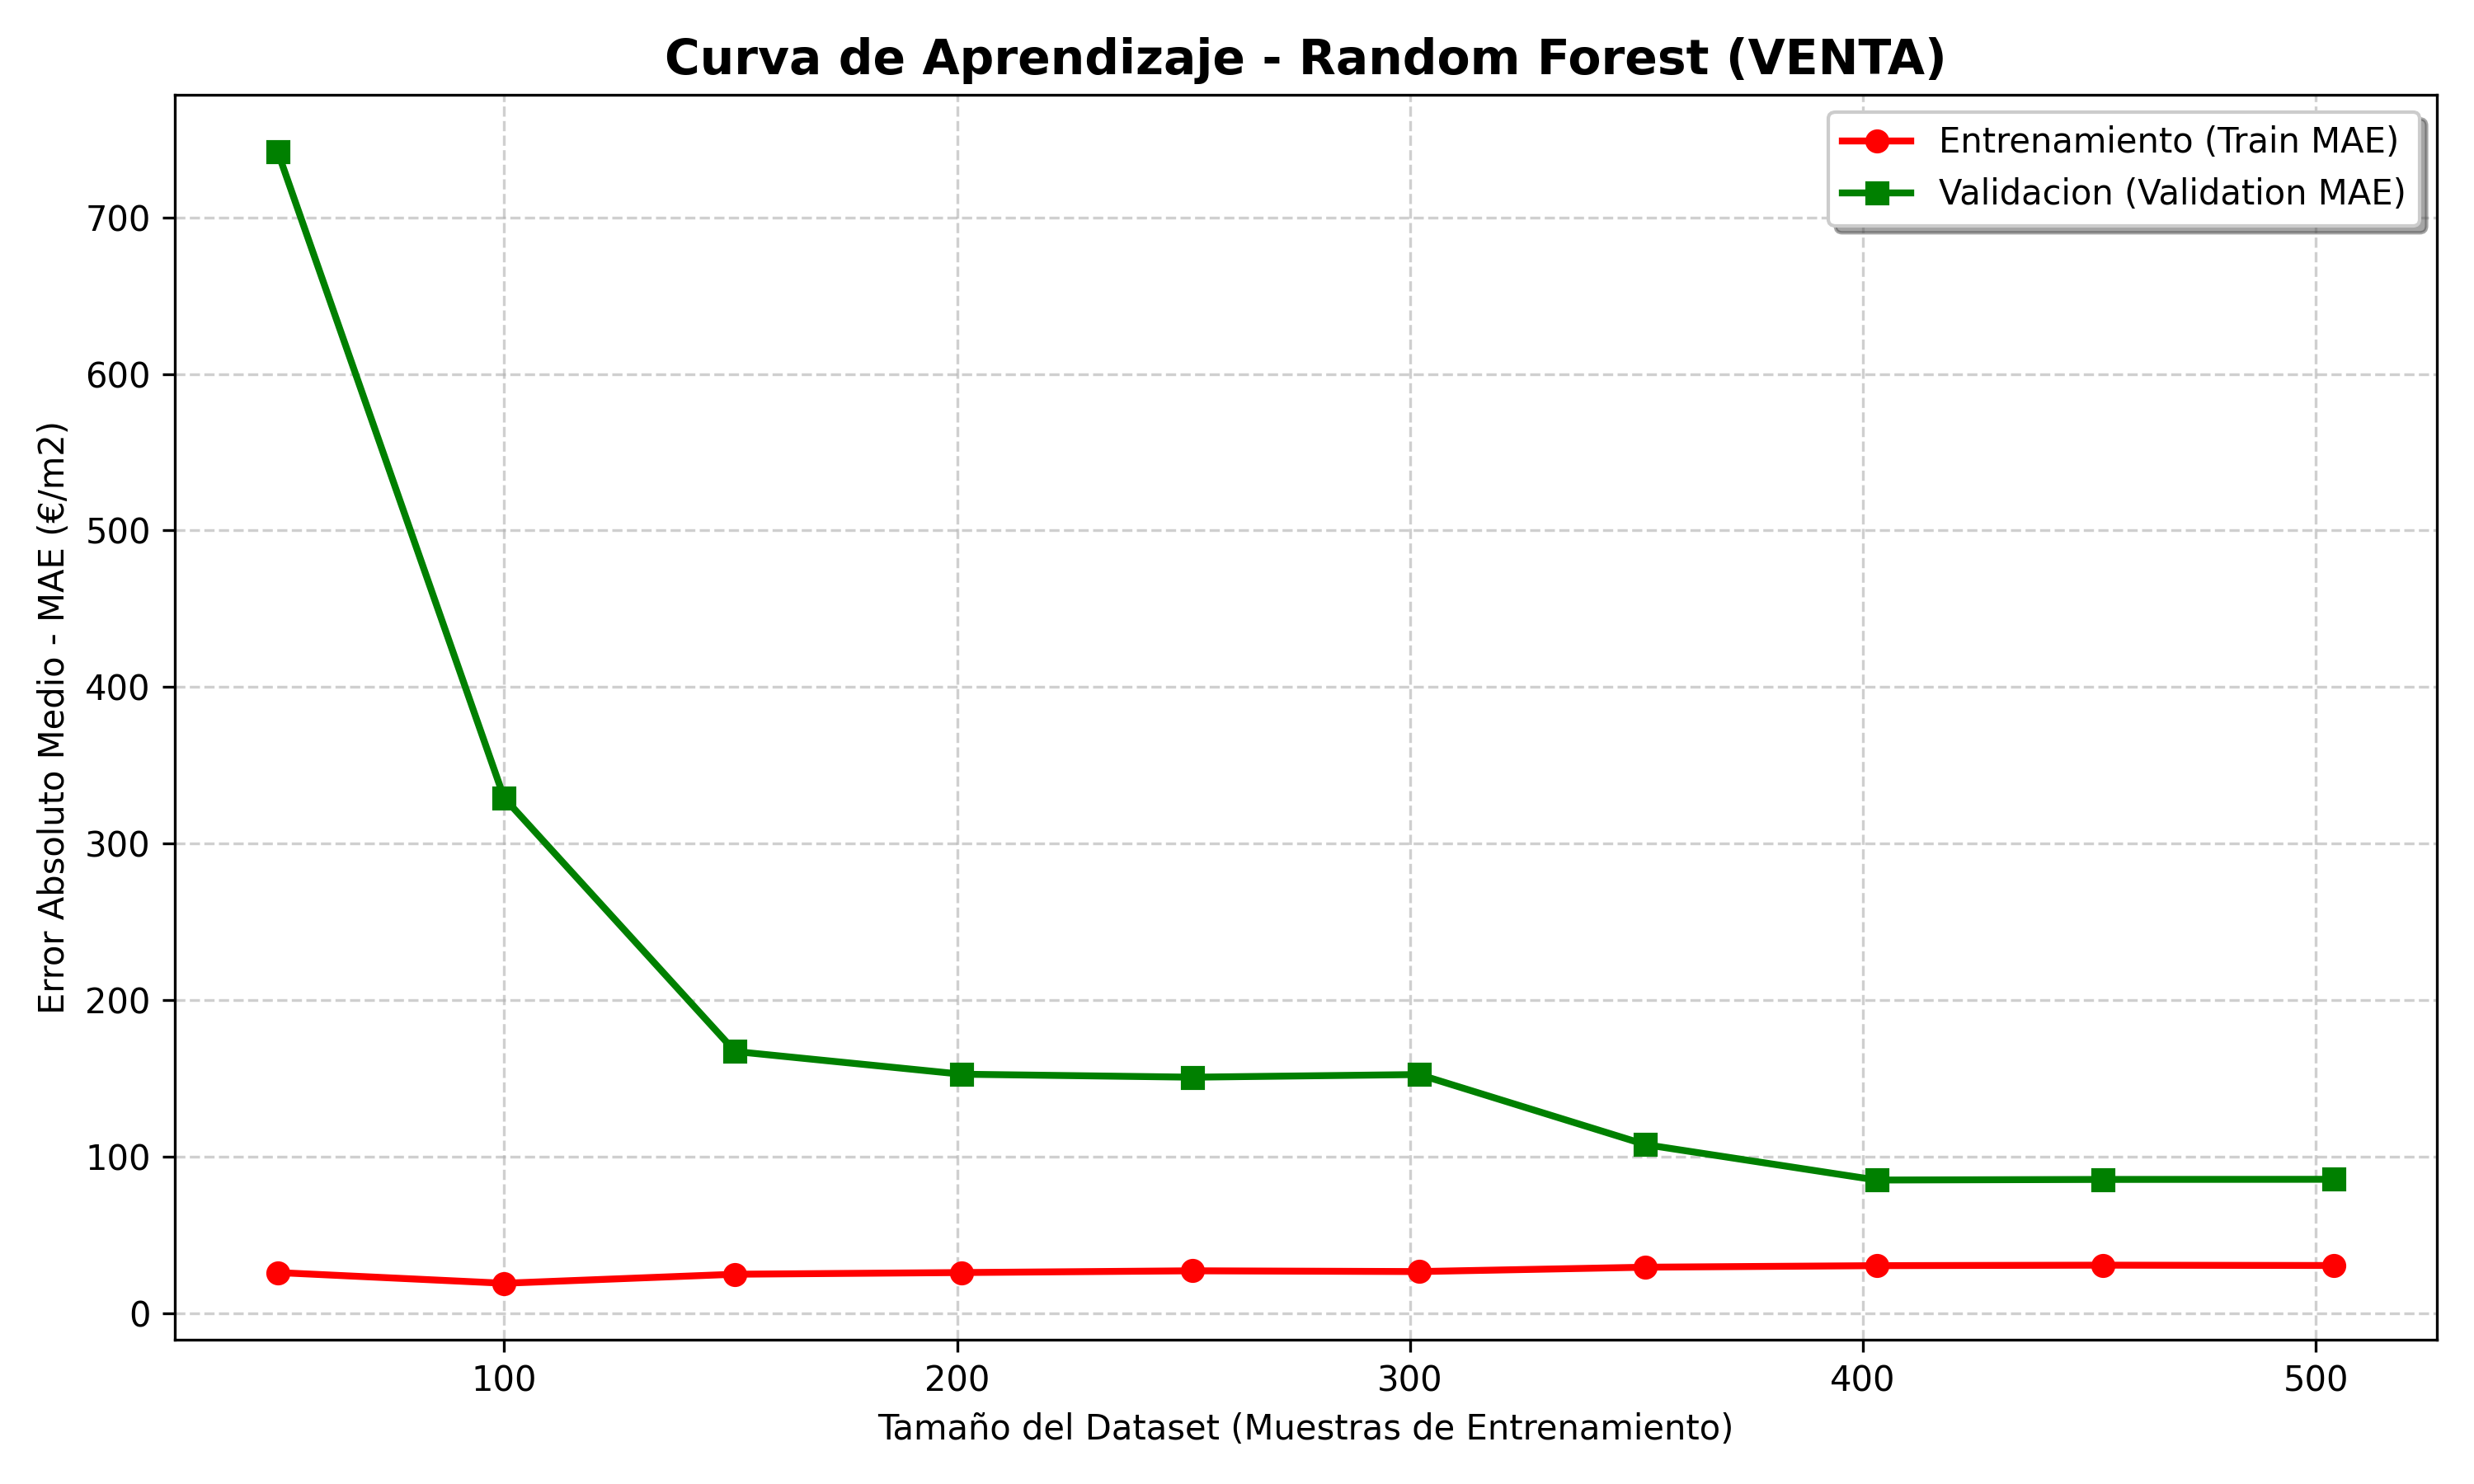
\includegraphics[width=0.40\linewidth]{img/phase3_learning_curve_random_forest_venta.png} & 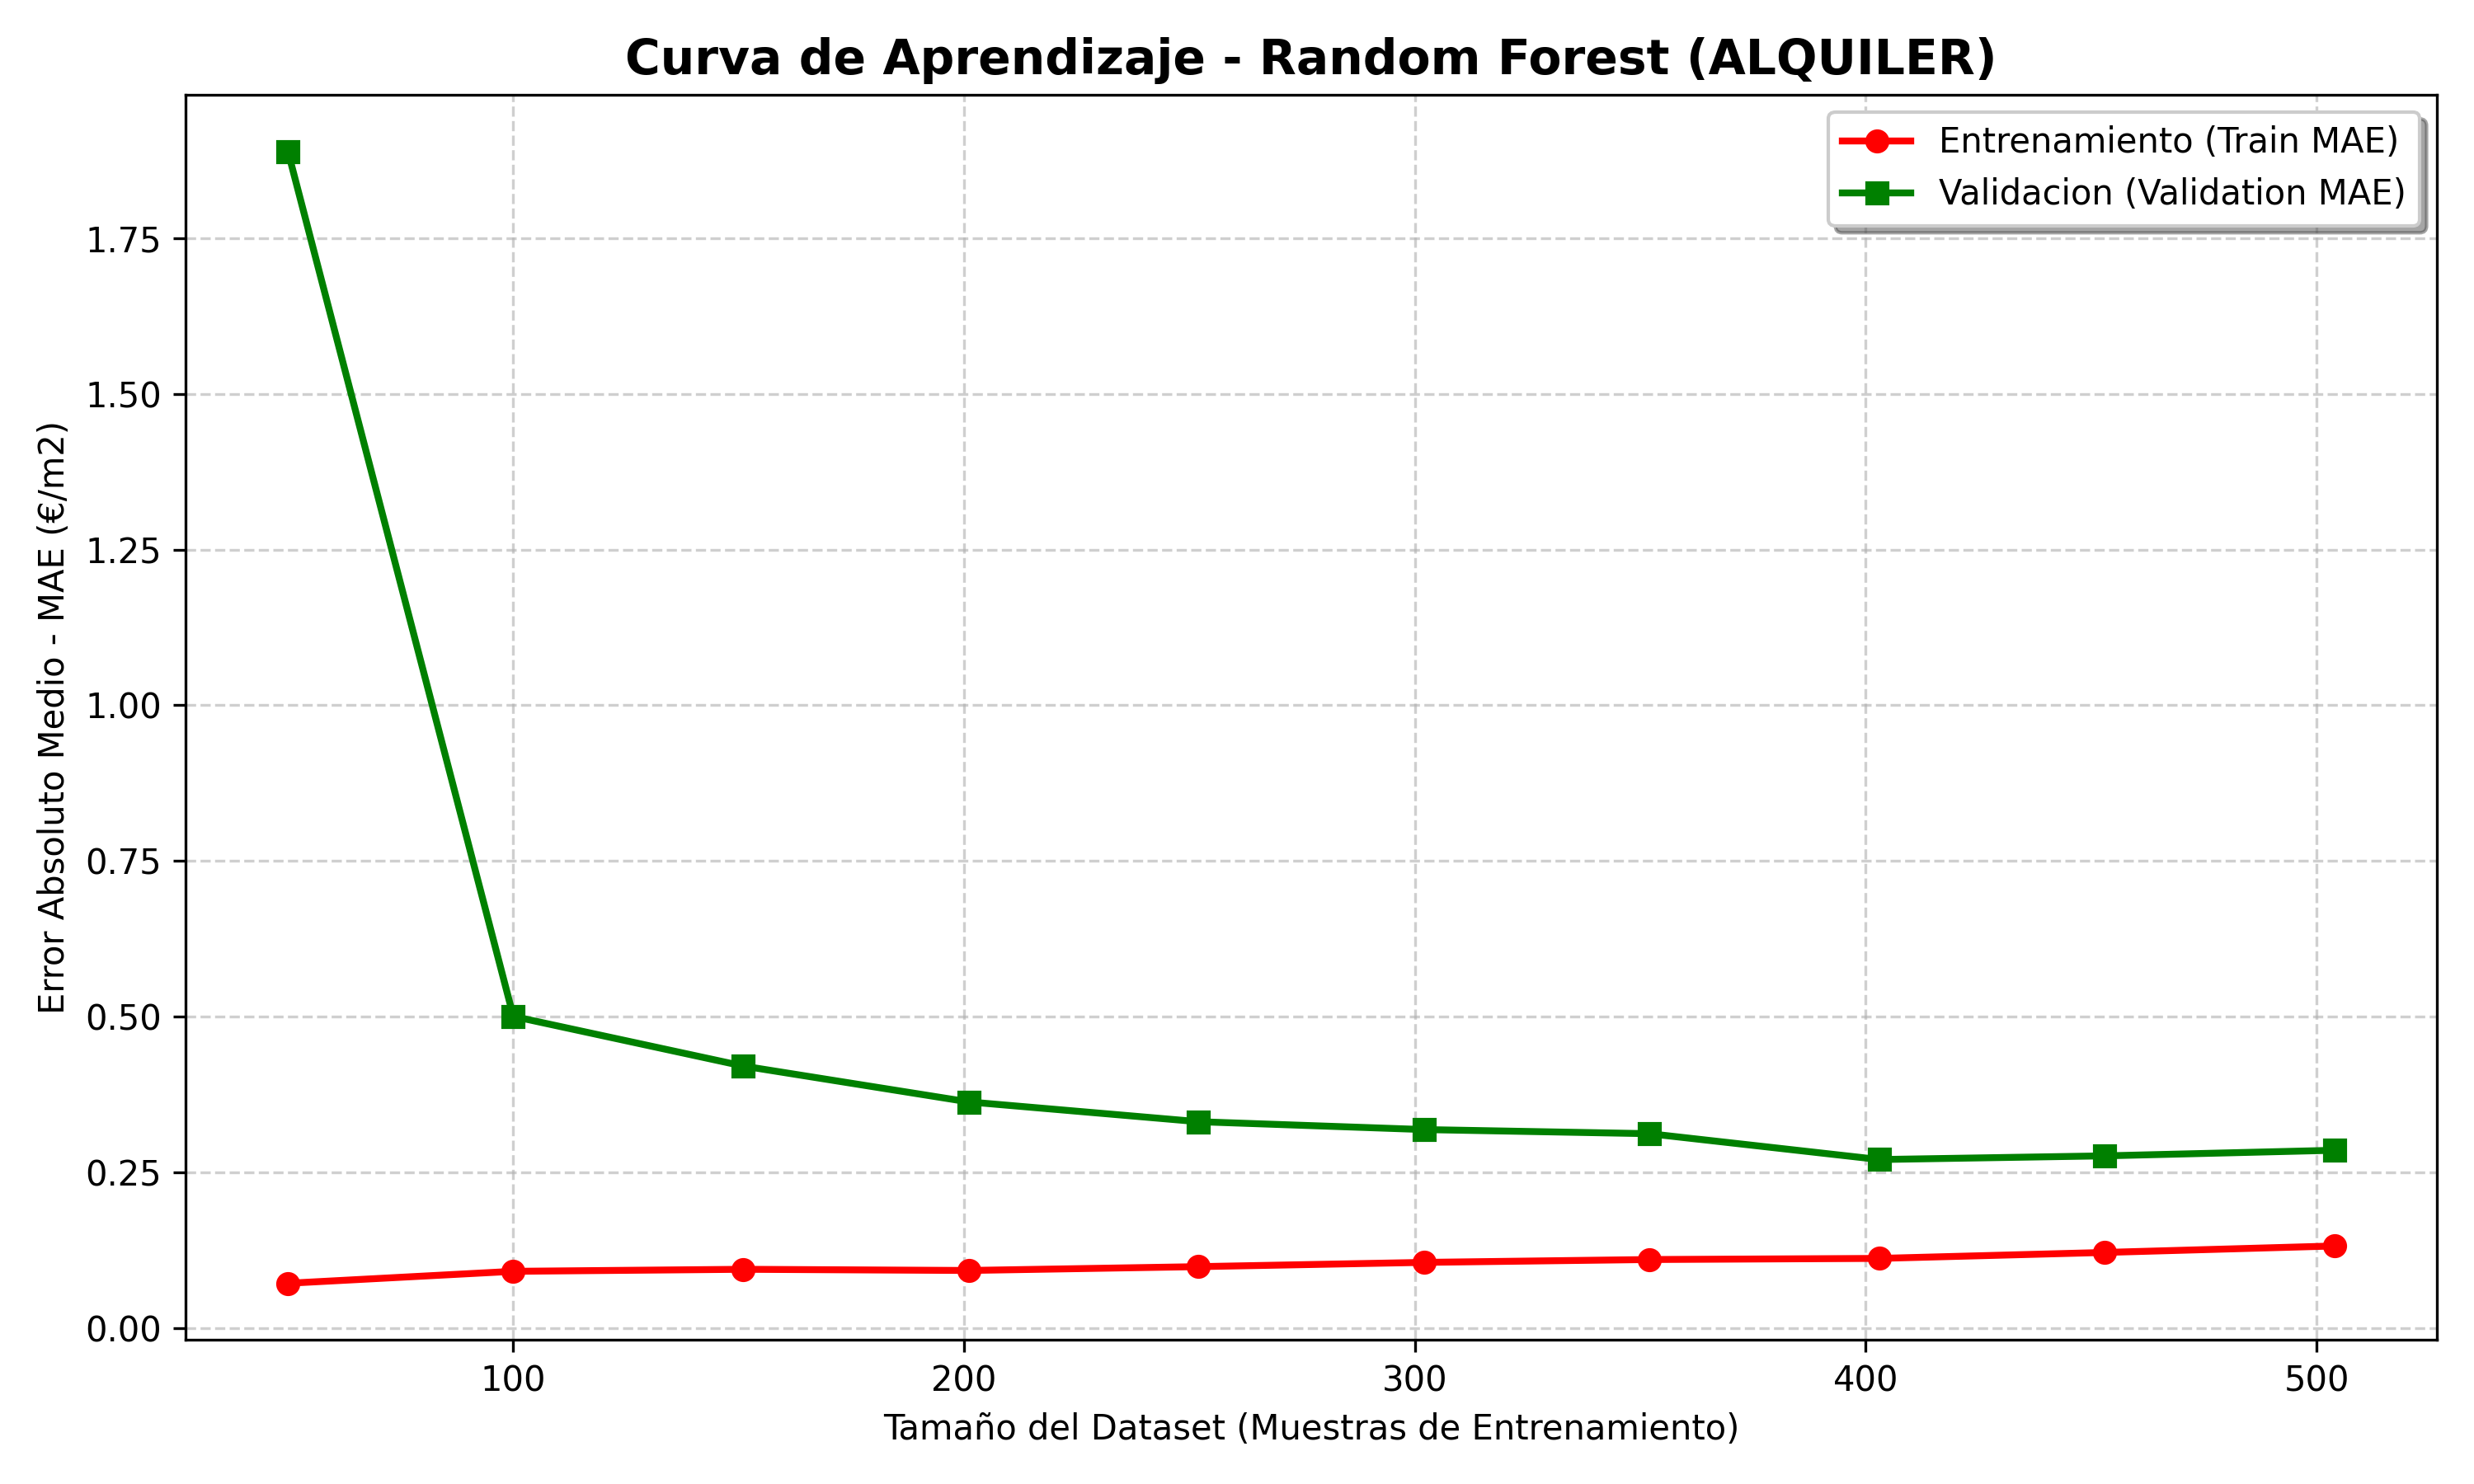
\includegraphics[width=0.40\linewidth]{img/phase3_learning_curve_random_forest_alquiler.png} \\
(a) Random Forest - Venta & (b) Random Forest - Alquiler \\
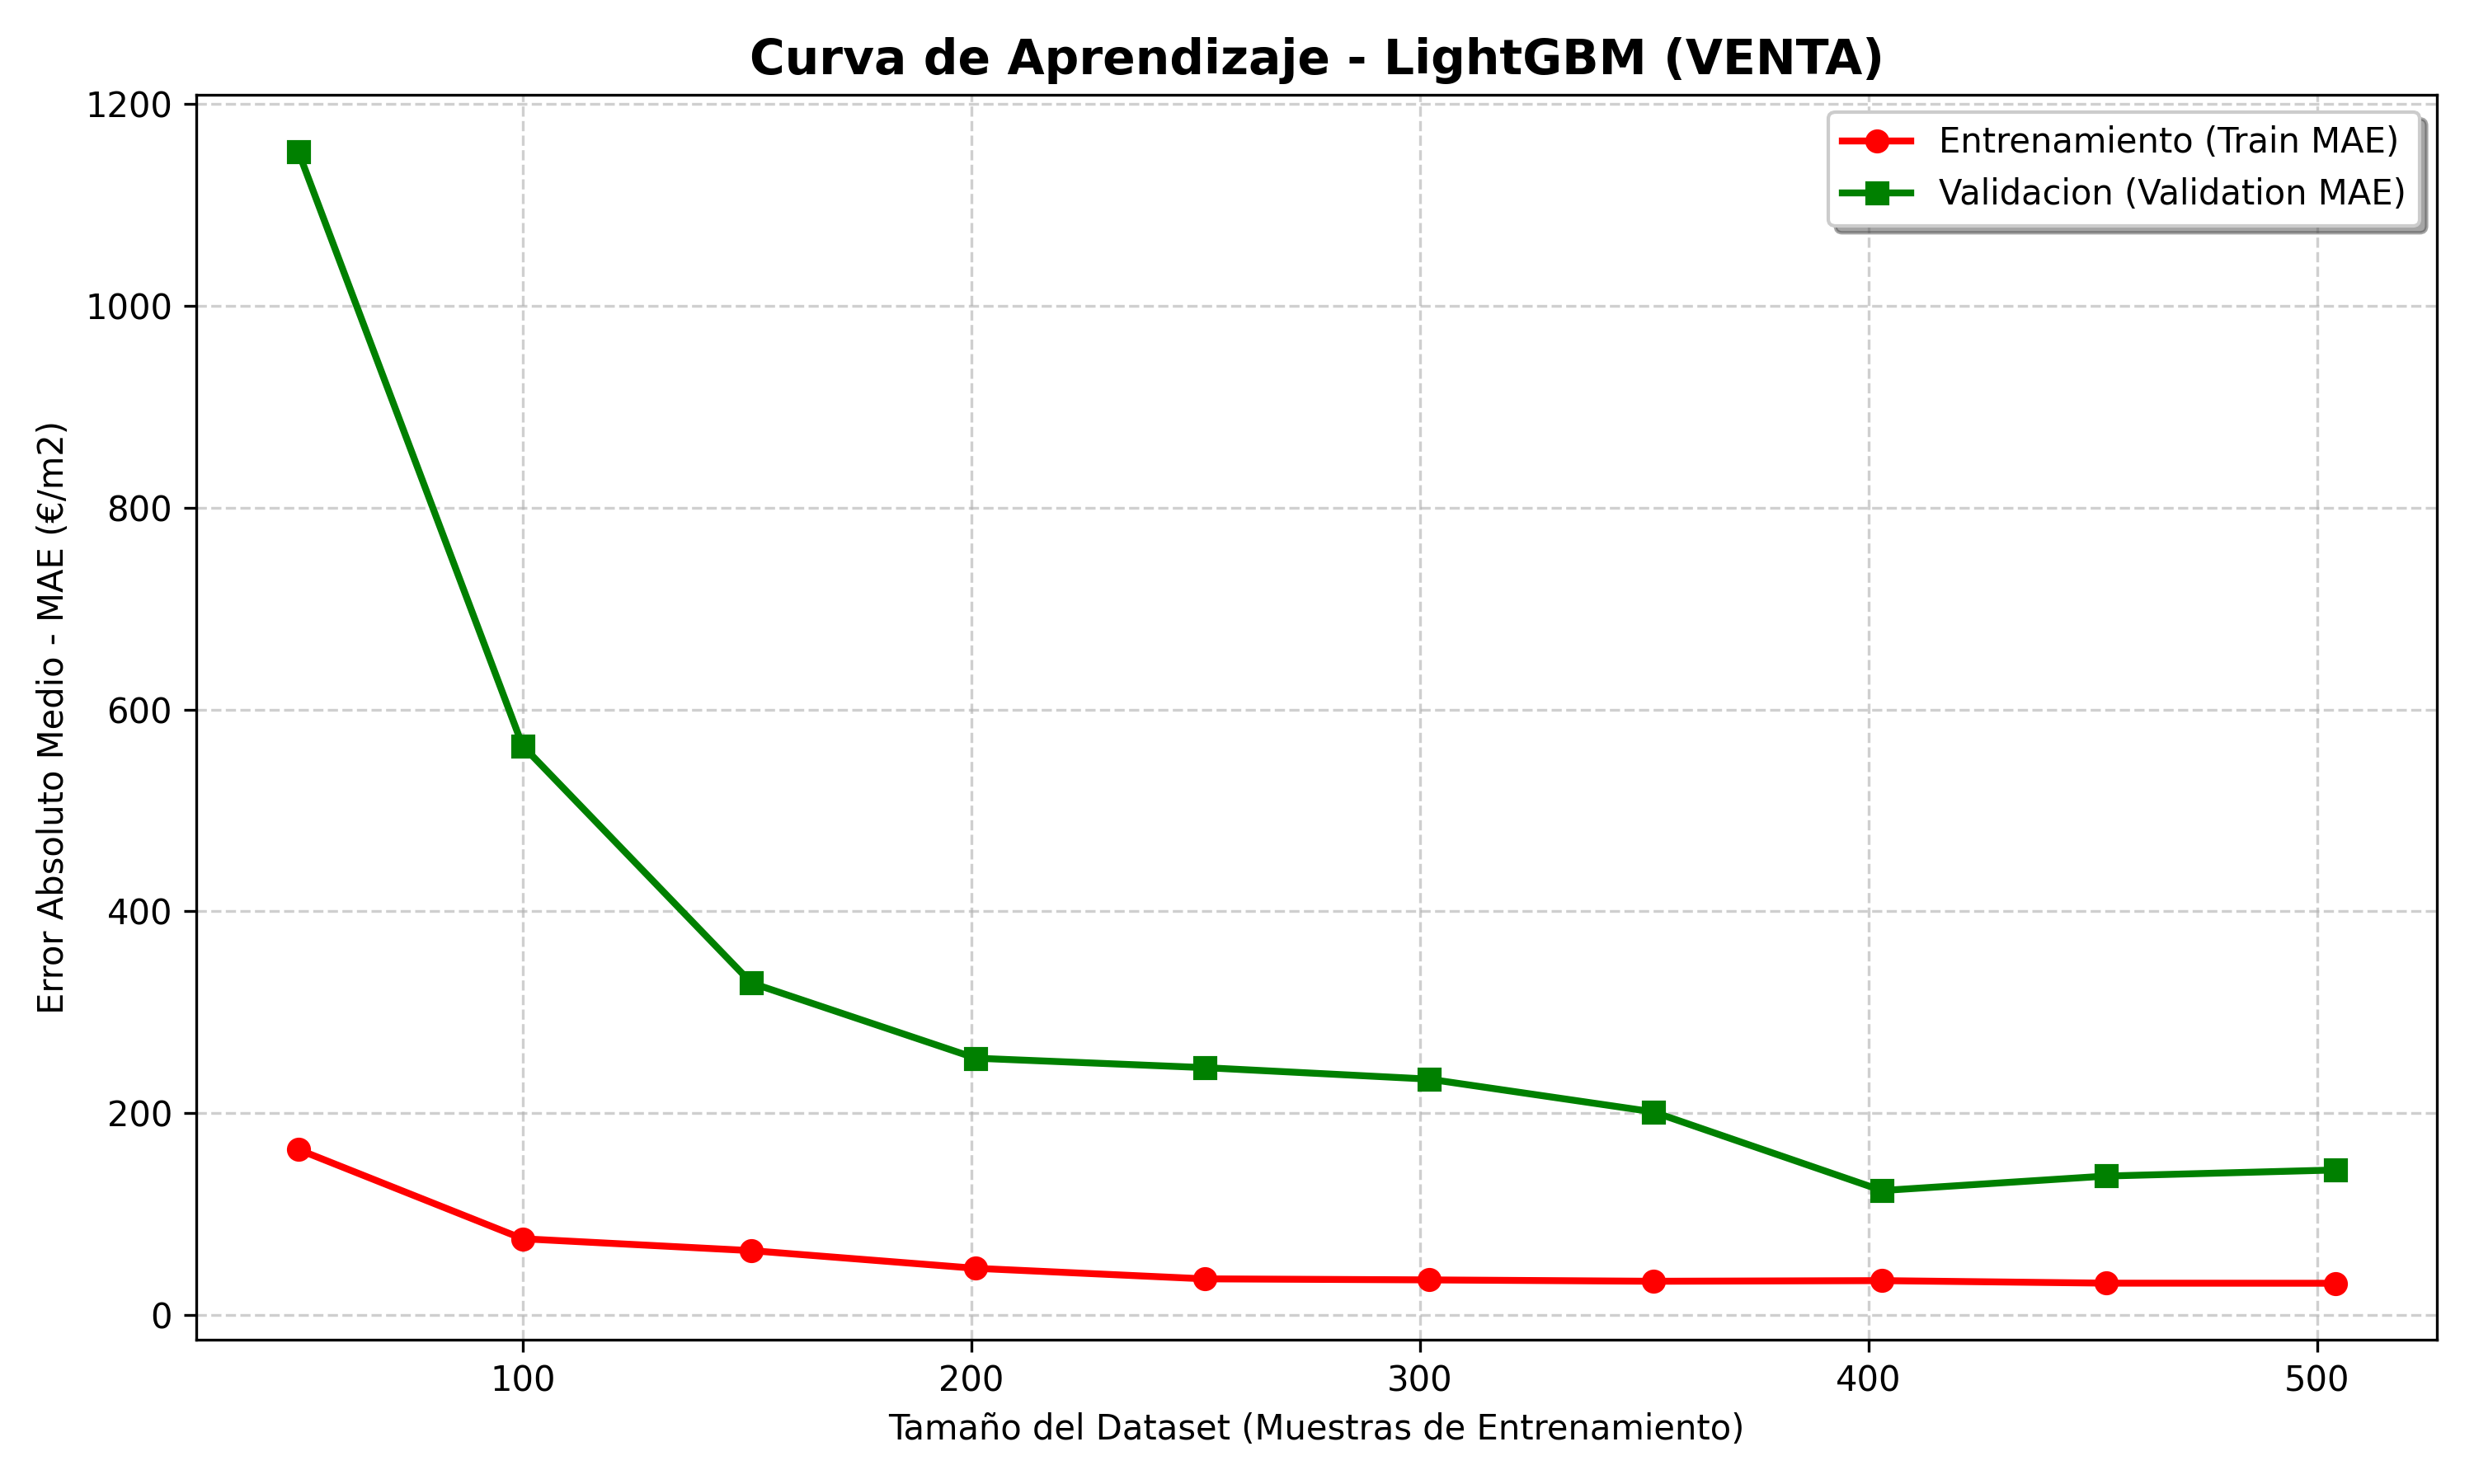
\includegraphics[width=0.40\linewidth]{img/phase3_learning_curve_lightgbm_venta.png} & 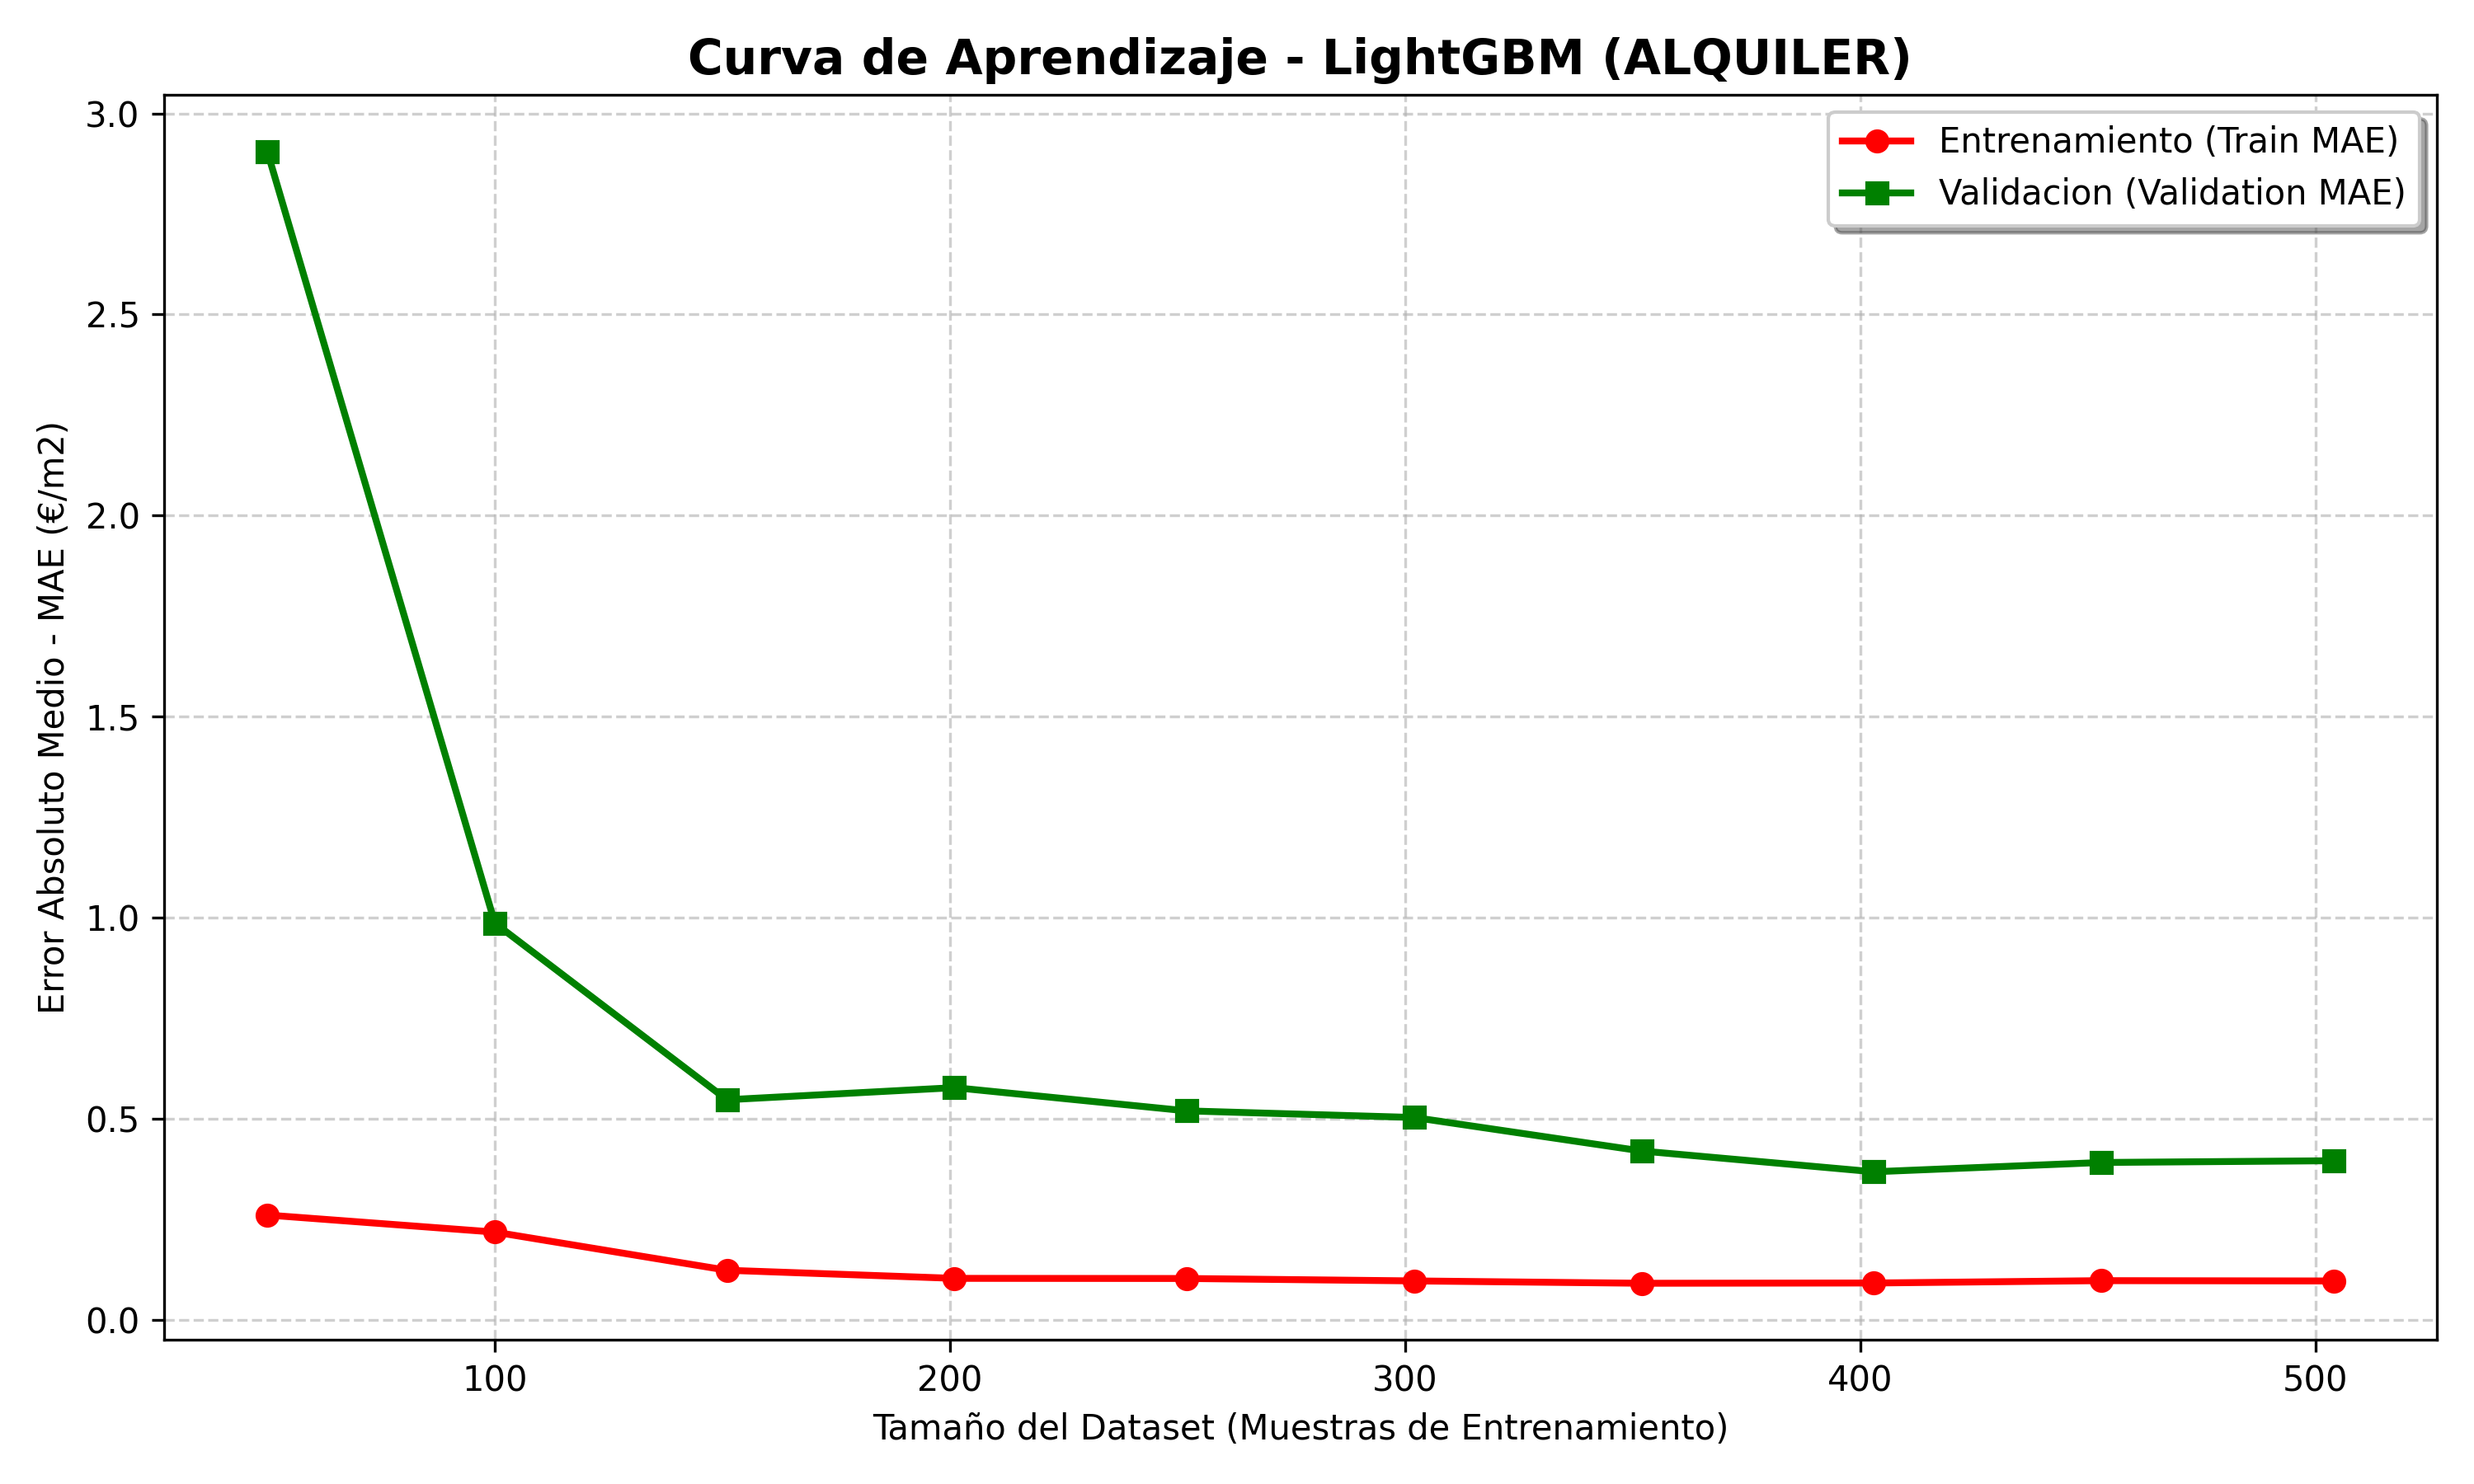
\includegraphics[width=0.40\linewidth]{img/phase3_learning_curve_lightgbm_alquiler.png} \\
(c) LightGBM - Venta & (d) LightGBM - Alquiler \\
\end{tabular}
\caption{Curvas de aprendizaje de Random Forest y LightGBM para los mercados de venta y alquiler en el modelado agregado de distrito.}
\label{fig:learning_curves_phase3_rf_lgb}
\end{figure}

\begin{figure}[H]
\centering
\begin{tabular}{cc}
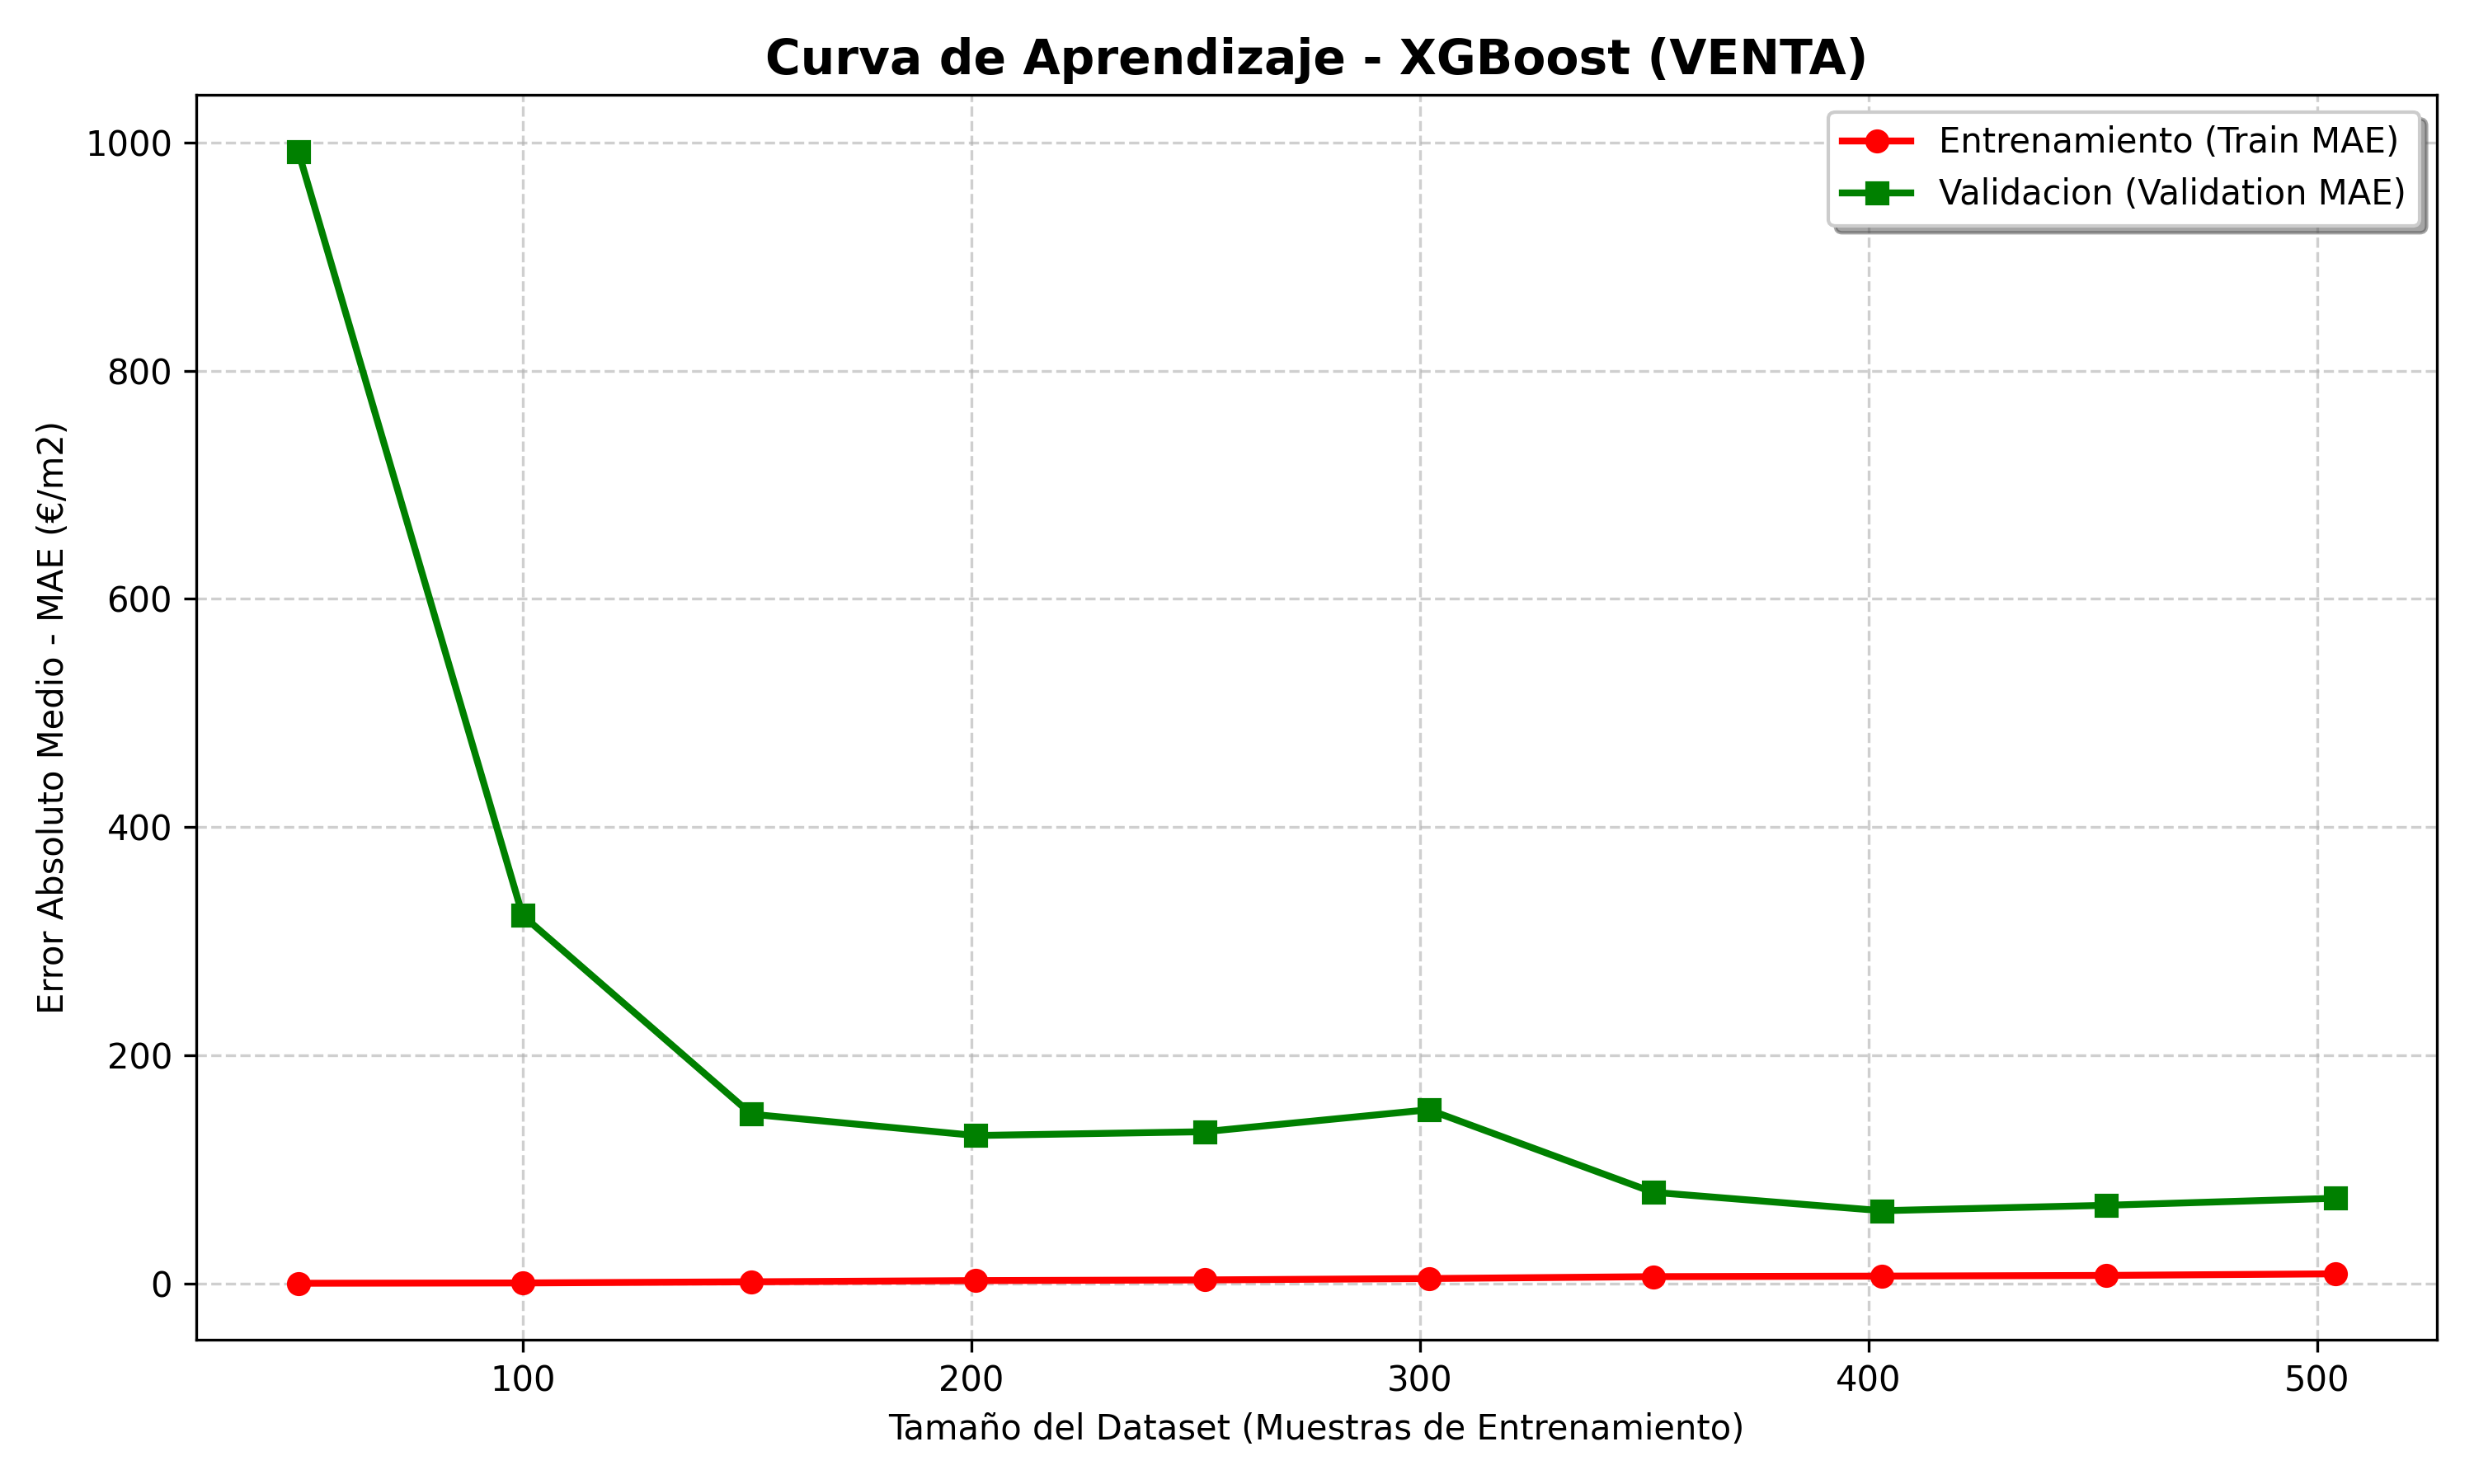
\includegraphics[width=0.40\linewidth]{img/phase3_learning_curve_xgboost_venta.png} & 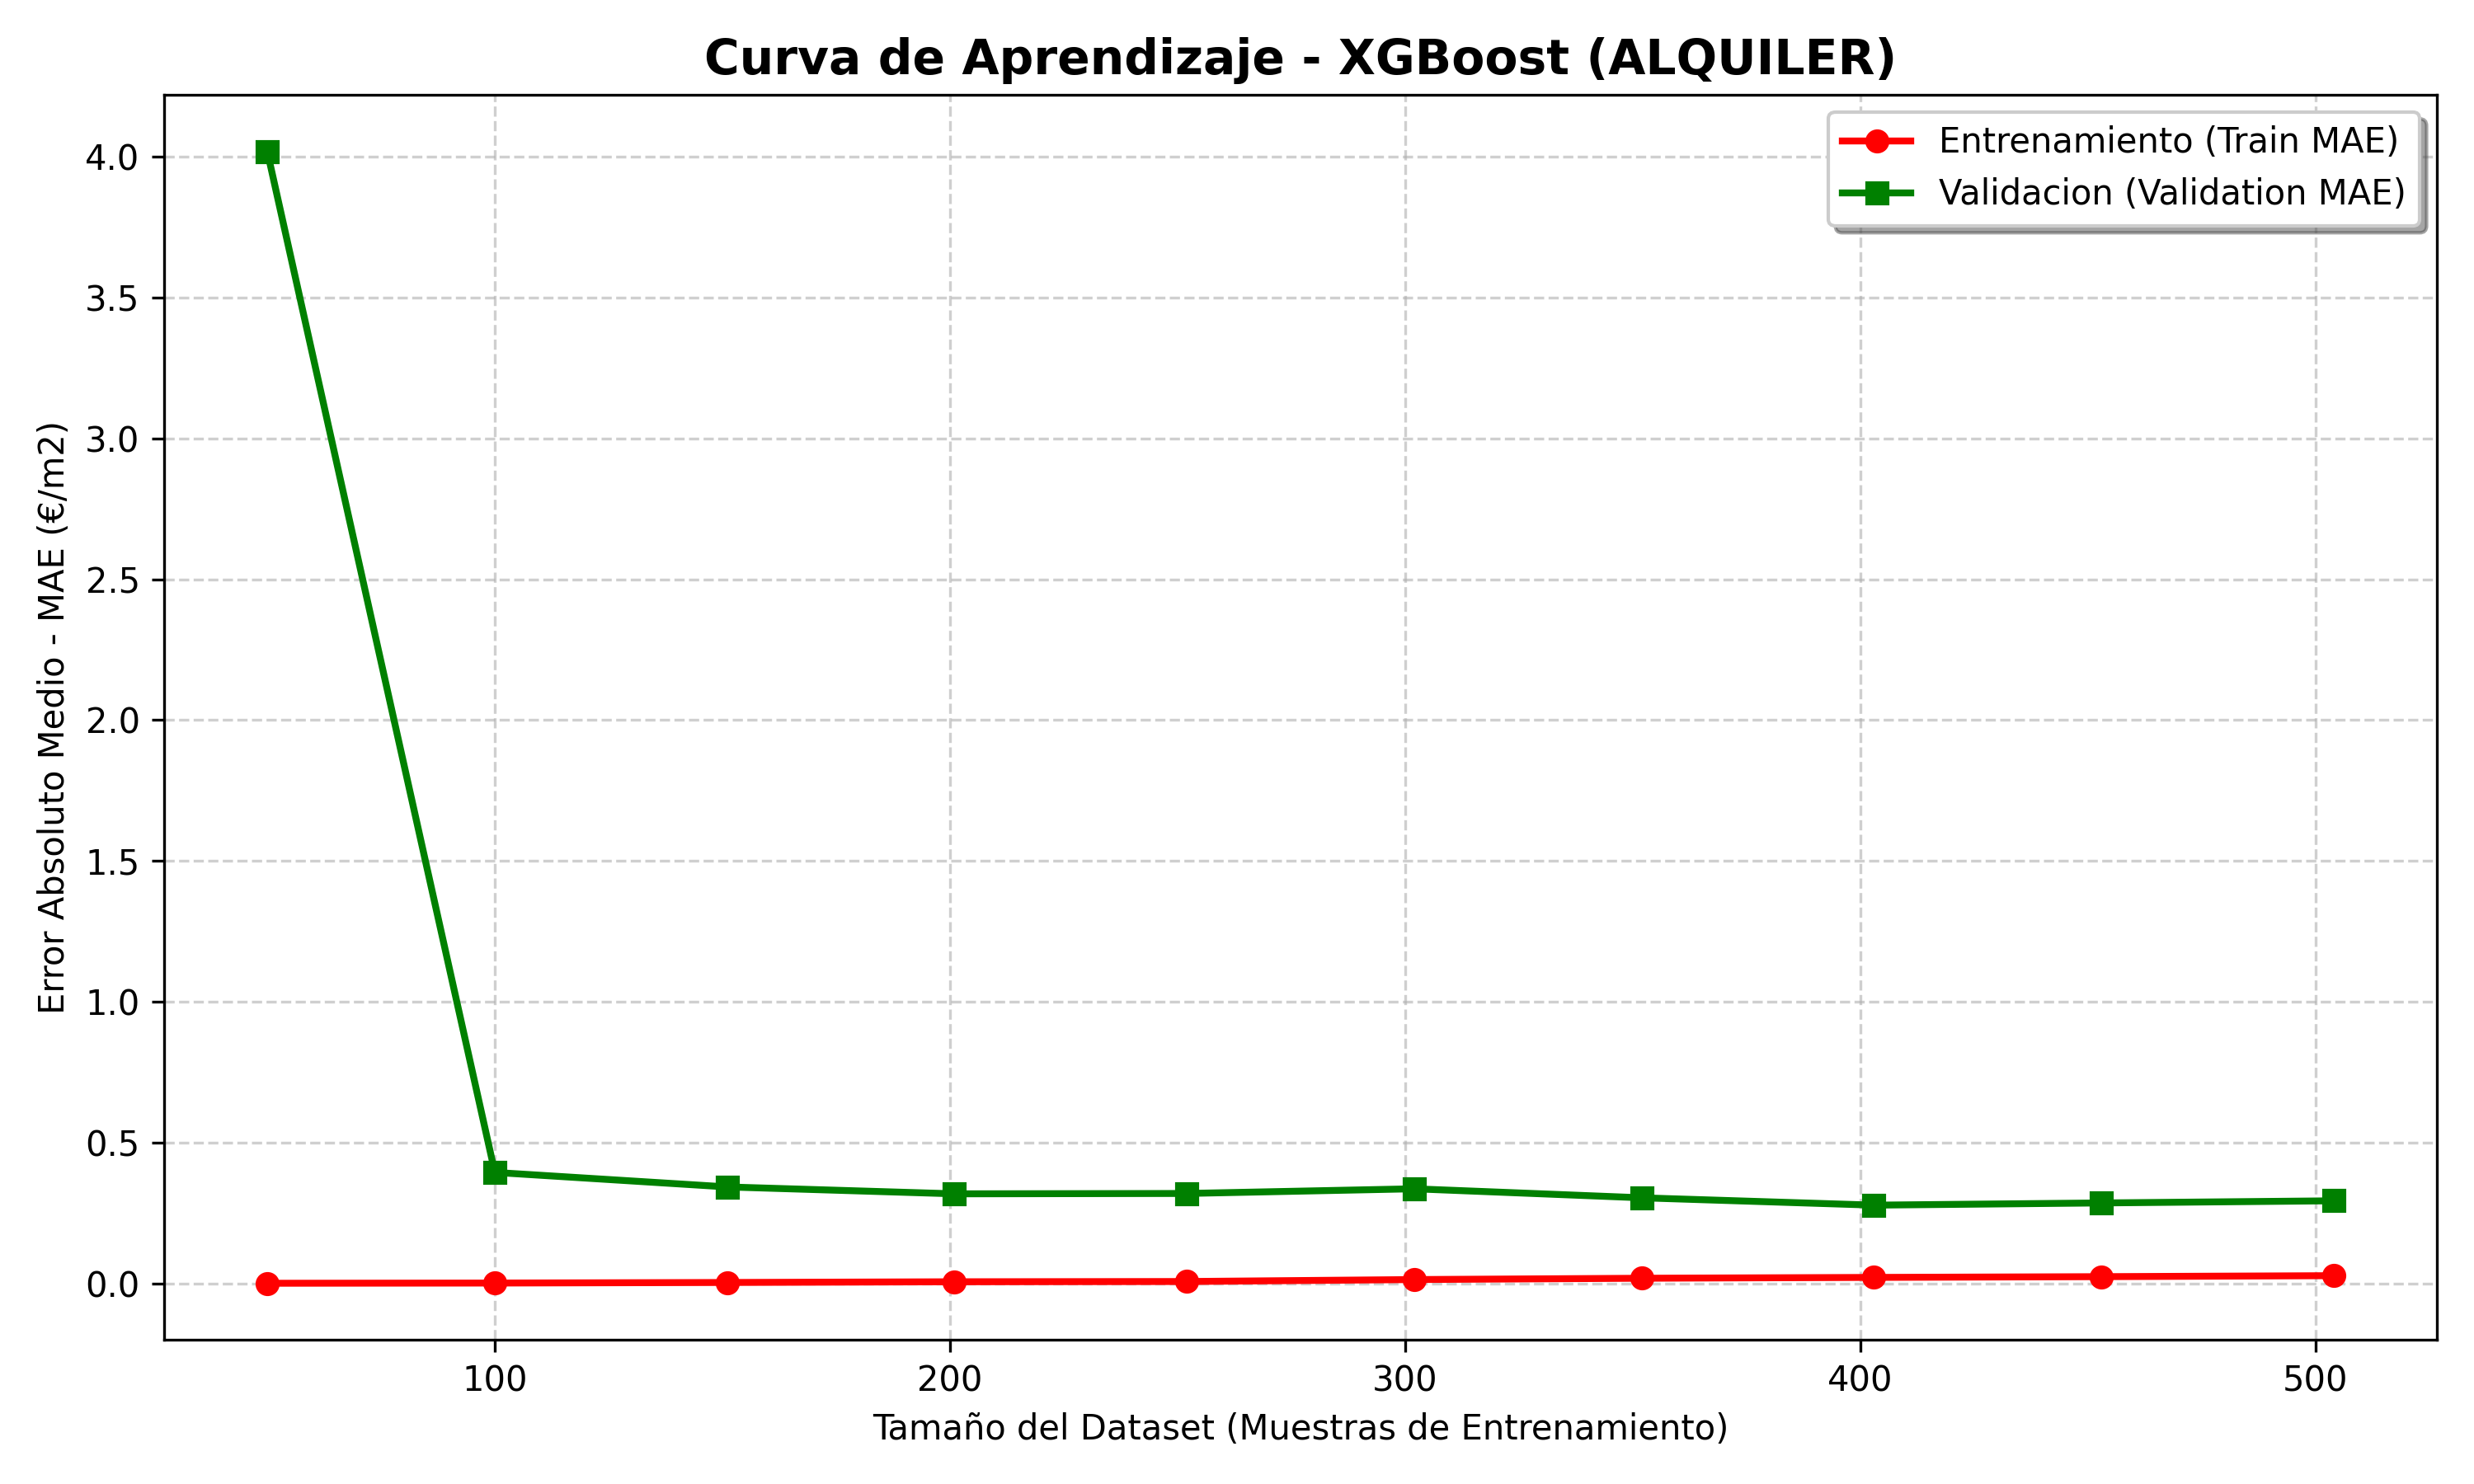
\includegraphics[width=0.40\linewidth]{img/phase3_learning_curve_xgboost_alquiler.png} \\
(a) XGBoost - Venta & (b) XGBoost - Alquiler \\
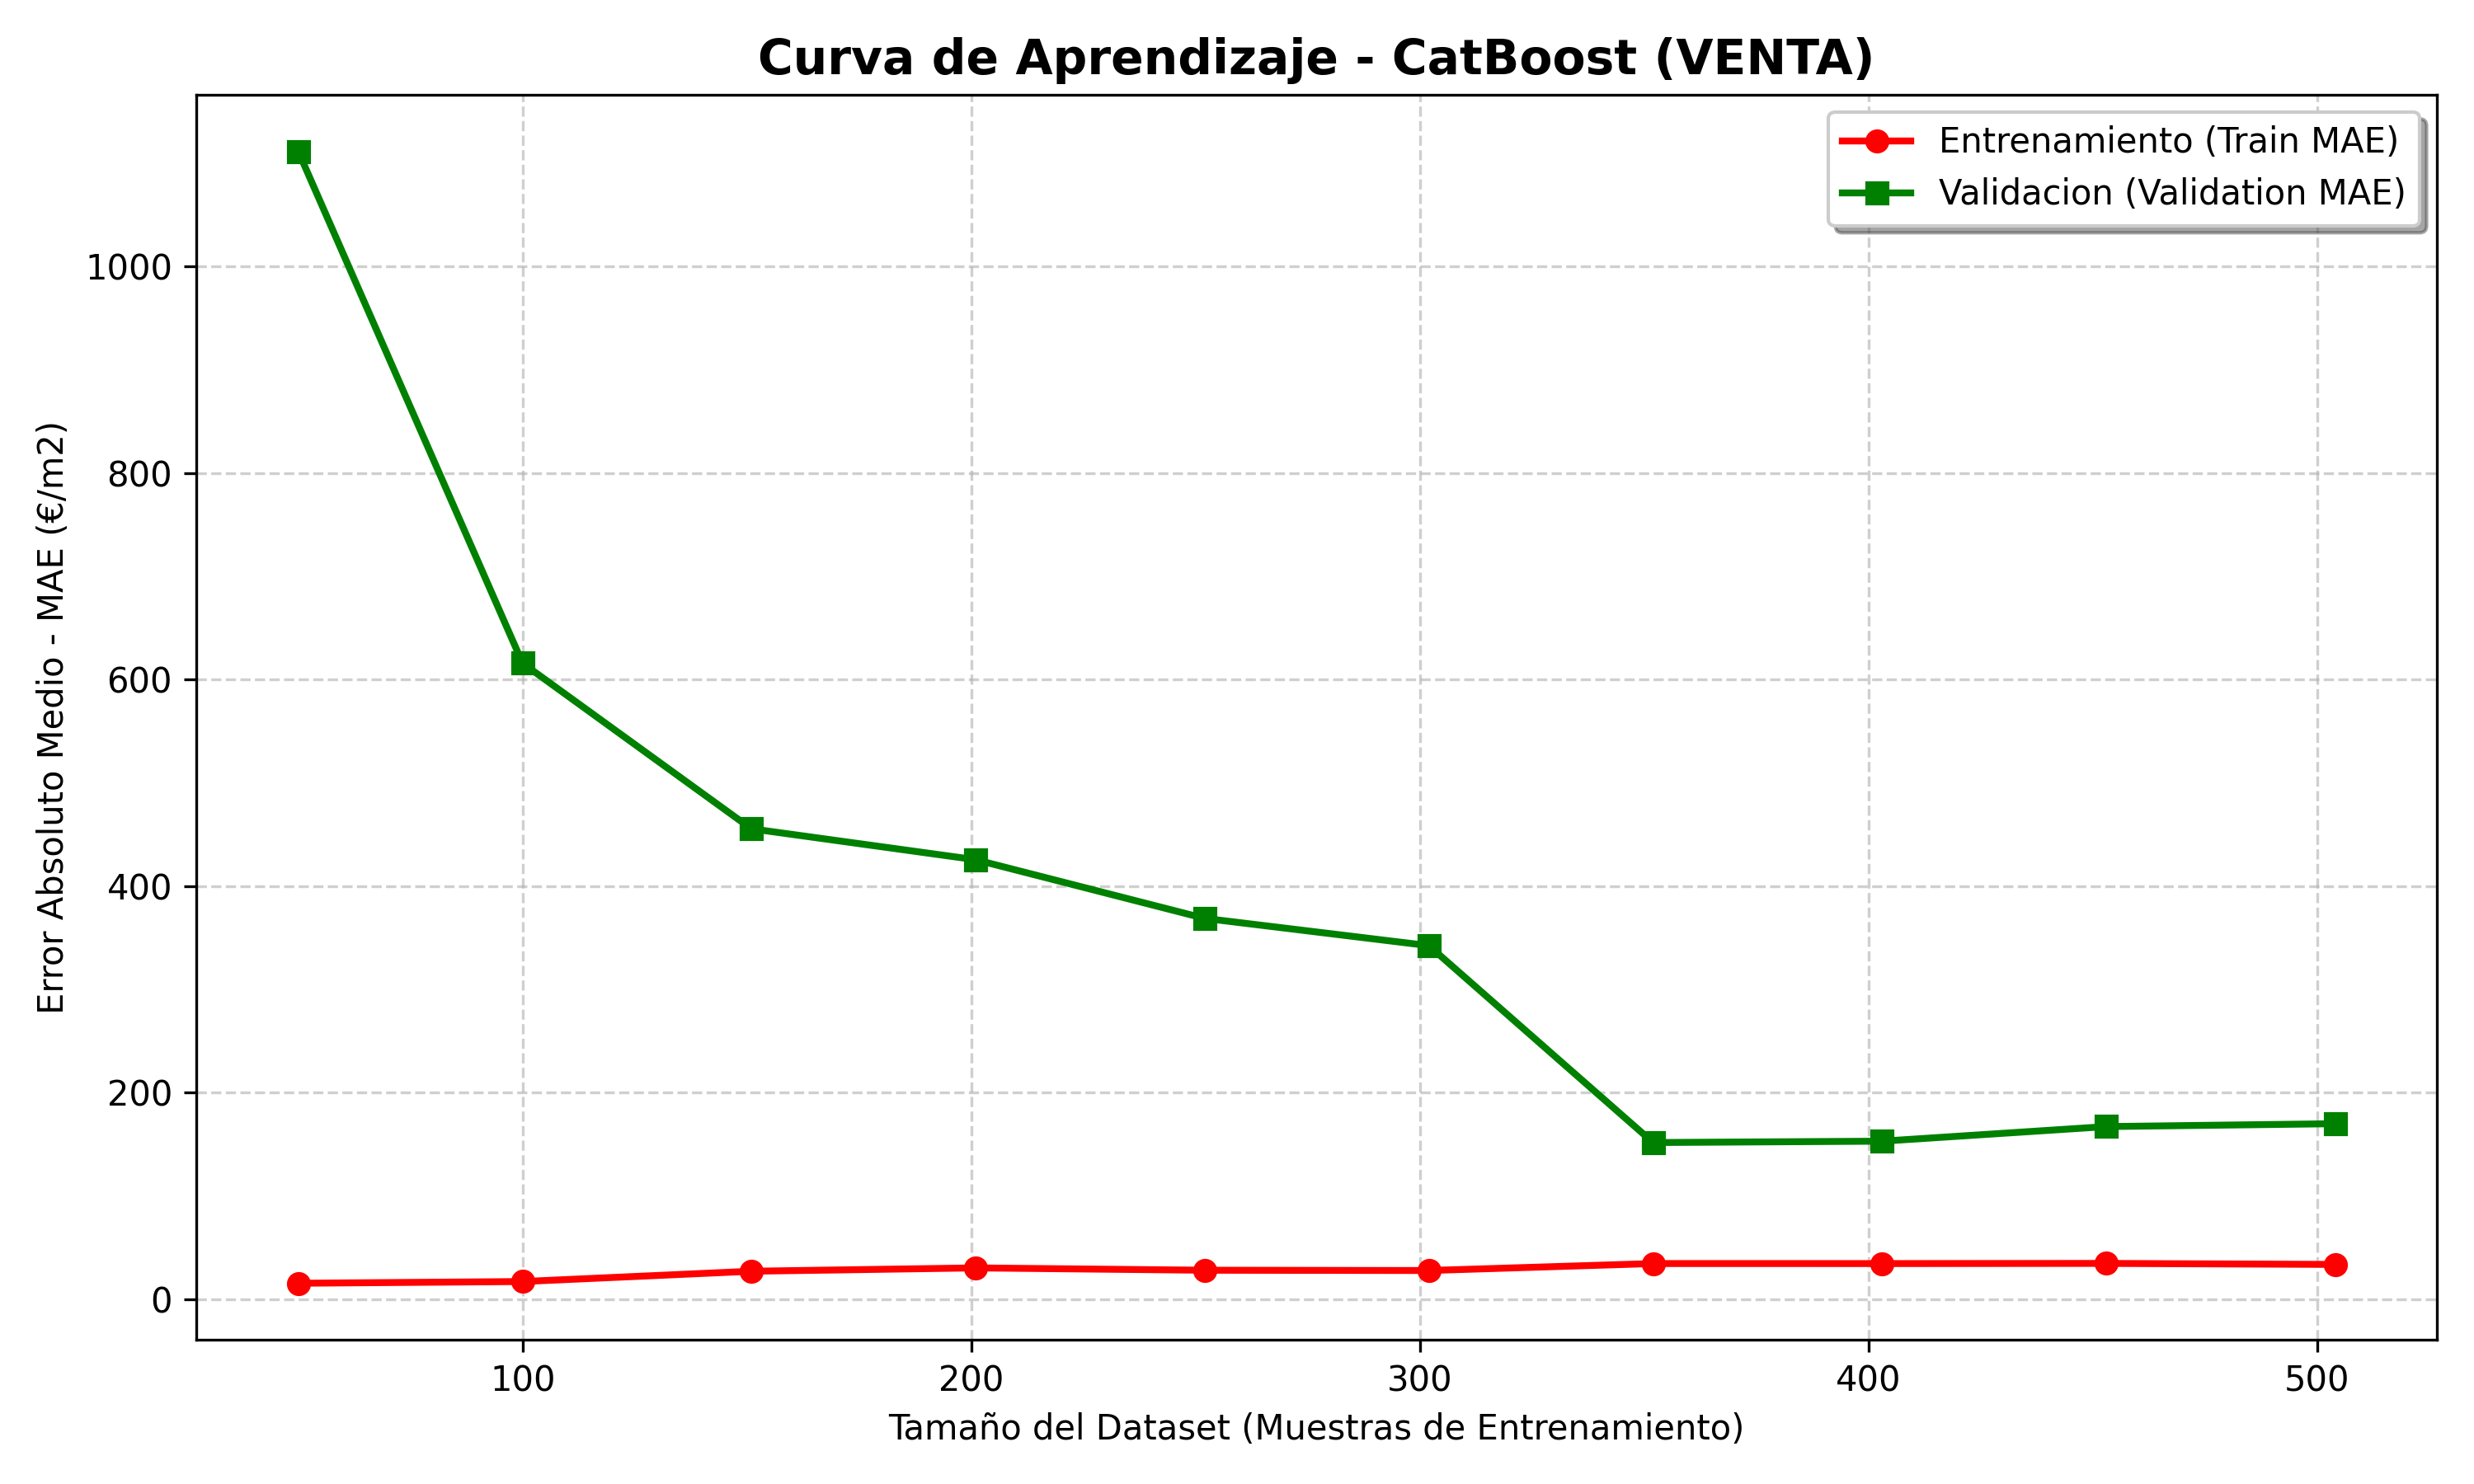
\includegraphics[width=0.40\linewidth]{img/phase3_learning_curve_catboost_venta.png} & 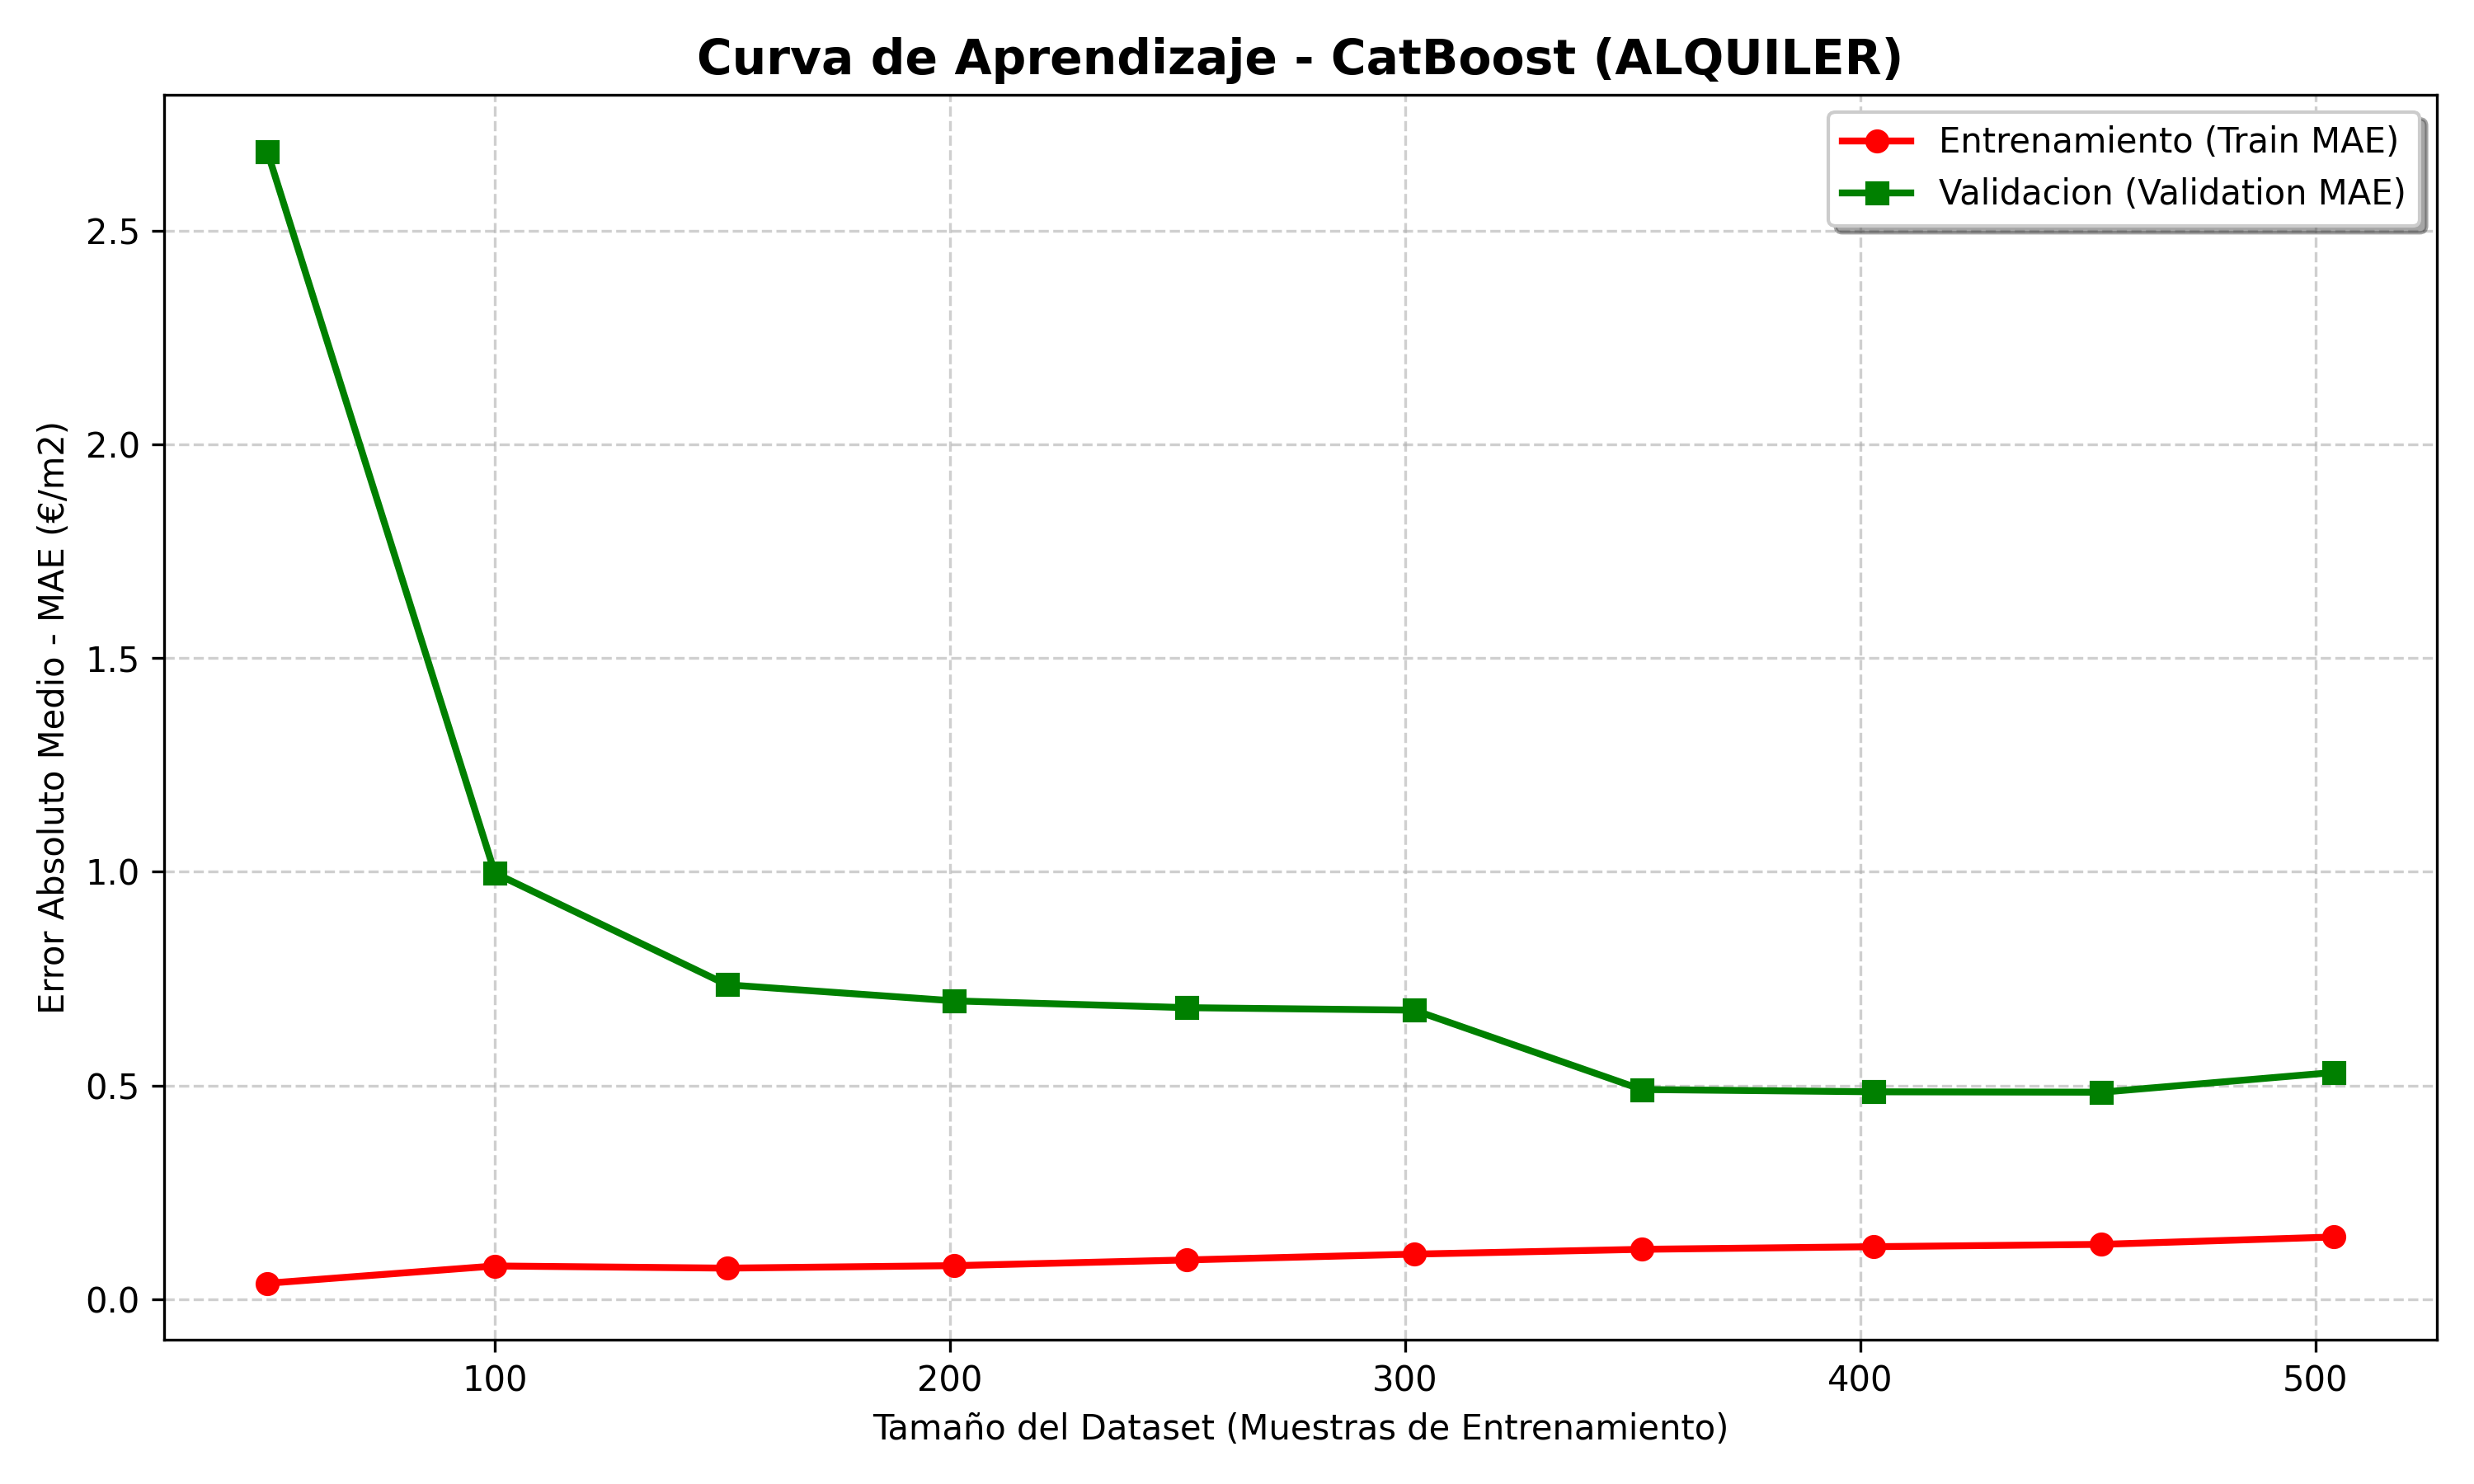
\includegraphics[width=0.40\linewidth]{img/phase3_learning_curve_catboost_alquiler.png} \\
(c) CatBoost - Venta & (d) CatBoost - Alquiler \\
\end{tabular}
\caption{Curvas de aprendizaje de XGBoost y CatBoost para los mercados de venta y alquiler en el modelado agregado de distrito.}
\label{fig:learning_curves_phase3_xgb_cat}
\end{figure}

Las curvas de aprendizaje a nivel de distrito (Figura~\ref{fig:learning_curves_phase3_rf_lgb} y Figura~\ref{fig:learning_curves_phase3_xgb_cat}) reflejan de manera clara el impacto de la agregación espacial en el entrenamiento. Al suavizarse la varianza de precios micro-local, las curvas de validación (línea verde) descienden rápidamente y muestran una convergencia veloz con la línea de entrenamiento (línea roja), estabilizándose a partir de un volumen de datos relativamente pequeño. En el mercado de venta, Random Forest y XGBoost se benefician fuertemente de esta agregación y convergen hacia cotas de error mínimas muy estables. En cambio, CatBoost y LightGBM muestran un ajuste más forzado debido a la pérdida de granularidad micro-local, con una brecha de generalización ligeramente mayor que la observada a nivel de barrio. Para el mercado de alquiler, las curvas muestran una convergencia uniforme para Random Forest, XGBoost y LightGBM con errores sumamente bajos, mientras que CatBoost se estabiliza con una meseta de error más elevada y un comportamiento relativamente indiferente a los incrementos de datos.

\section{Fase de Optimización: Entrenamiento con Dataset Enriquecido}
Establecida la fase comparativa base a nivel micro-local de barrio, la etapa principal del modelado predictivo se orientó al desarrollo de la Fase de Producción Enriquecida. Esta fase se entrena a escala micro-local de barrio (\texttt{id\_barrio != -1}) debido a que, al disponer de una mayor densidad de datos y variables de contexto geográfico, facilita la captura de patrones territoriales finos de forma mucho más precisa. La hipótesis fundamental de esta fase de optimización y enriquecimiento se basa en que los precios de las viviendas no se explican únicamente por factores puramente internos del inmueble o su localización geográfica básica (como la superficie construida, la ubicación en un determinado barrio o distrito o la inercia temporal simple). Por el contrario, el mercado inmobiliario responde a un sistema dinámico e influenciado de manera directa por factores macroeconómicos y socioeconómicos externos (tales como la evolución de los tipos de interés, la renta media disponible por hogar, la liquidez transaccional de compraventas y las condiciones del crédito hipotecario). Si bien es matemáticamente imposible determinar la totalidad de las variables externas que intervienen en la conformación de precios, la inyección en los algoritmos de este conjunto de indicadores contextuales enriquecidos ayuda a dotar a los modelos de una mayor sensibilidad y capacidad predictiva frente a shocks y perturbaciones del mercado, aun a costa de incrementar levemente la complejidad del aprendizaje.

Para evaluar de forma justa y científicamente rigurosa a todos los algoritmos, se entrenaron los cuatro modelos (XGBoost, LightGBM, Random Forest y CatBoost) en un flujo secuencial estructurado en tres fases lógicas progresivas (Fase A, Fase B y Fase C), con un entrenamiento ciego estrictamente hasta diciembre de 2025, tal como se realizó en las fases previas, y con validación out-of-sample sobre los meses de 2026 (enero, febrero, marzo), los cuales sirvieron exclusivamente como conjunto de test para contrastar las proyecciones frente a los valores reales. Para evitar el sobreajuste y optimizar los tiempos de cómputo en fases donde el error tiende a estabilizarse o no presenta mejoras progresivas claras, se configuró un límite de parada temprana (\textit{early stopping}) de 50 iteraciones para todos los modelos, basándose en el comportamiento observado en los experimentos previos.

\subsection{Fase A: Línea Base Enriquecida (Cruce de Datos Socioeconómicos y Macroeconómicos)}
La primera fase consistió en inyectar el dataset completo y enriquecido consolidado en el DataMart dimensional. Para cada registro en bruto de barrio y distrito, se incorporaron:
\begin{enumerate}
    \item \textbf{Variables Macroeconómicas Mensuales:} Ingesta mensual del tipo de interés medio y del importe medio de las hipotecas constituidas del Banco de España, capturando el coste del financiamiento hipotecario.
    \item \textbf{Liquidez Registral:} Ingesta mensual del volumen de transacciones de compraventa del Colegio de Registradores de España para modelar la velocidad del mercado de cada distrito.
    \item \textbf{Indicador Socioeconómico Local:} Cruce de la Renta Neta Media por Hogar (INE) a nivel de barrio para mapear el poder adquisitivo territorial.
\end{enumerate}

\begin{table}[H]
\centering
\caption{Matriz de rendimiento comparativa: Fase A - Línea Base Enriquecida - Mercado de Venta (€/m\textsuperscript{2})}
\label{tab:fasea_venta}
\resizebox{\textwidth}{!}{%
\begin{tabular}{|l|c|c|c|c|c|c|c|c|c|c|c|}
\hline
\textbf{Algoritmo} & \textbf{MAE} & \textbf{RMSE} & \textbf{R\textsuperscript{2}} & \textbf{MAPE} & \textbf{Sesgo} & \textbf{MAE} & \textbf{R\textsuperscript{2}} & \textbf{MAE} & \textbf{R\textsuperscript{2}} & \textbf{T. Train} & \textbf{T. Pred} \\
 & \textbf{Global} & \textbf{Global} & \textbf{Global} & \textbf{Global (\%)} & \textbf{Global} & \textbf{Salamanca} & \textbf{Salamanca} & \textbf{C. Lineal} & \textbf{C. Lineal} & \textbf{(s)} & \textbf{(s)} \\
\hline
\textbf{Random Forest} & \textbf{99,97} & \textbf{138,52} & \textbf{0,9955} & \textbf{1,87\%} & 24,47 & 112,50 & 0,9707 & \textbf{146,27} & \textbf{0,9852} & 1,164 & 0,043 \\
\textbf{LightGBM} & 102,82 & 143,28 & 0,9952 & 1,92\% & 13,23 & \textbf{73,35} & \textbf{0,9843} & 227,51 & 0,9650 & \textbf{0,361} & 0,003 \\
\textbf{XGBoost} & 116,08 & 171,82 & 0,9931 & 2,12\% & \textbf{-4,69} & 79,58 & 0,9727 & 255,29 & 0,9591 & 0,452 & 0,004 \\
\textbf{CatBoost} & 129,53 & 182,23 & 0,9923 & 2,33\% & -34,77 & 127,03 & 0,9718 & 327,28 & 0,9435 & 1,451 & \textbf{0,002} \\
\hline
\end{tabular}%
}
\end{table}

\begin{table}[H]
\centering
\caption{Matriz de rendimiento comparativa: Fase A - Línea Base Enriquecida - Mercado de Alquiler (€/m\textsuperscript{2})}
\label{tab:fasea_alquiler}
\resizebox{\textwidth}{!}{%
\begin{tabular}{|l|c|c|c|c|c|c|c|c|c|c|c|}
\hline
\textbf{Algoritmo} & \textbf{MAE} & \textbf{RMSE} & \textbf{R\textsuperscript{2}} & \textbf{MAPE} & \textbf{Sesgo} & \textbf{MAE} & \textbf{R\textsuperscript{2}} & \textbf{MAE} & \textbf{R\textsuperscript{2}} & \textbf{T. Train} & \textbf{T. Pred} \\
 & \textbf{Global} & \textbf{Global} & \textbf{Global} & \textbf{Global (\%)} & \textbf{Global} & \textbf{Salamanca} & \textbf{Salamanca} & \textbf{C. Lineal} & \textbf{C. Lineal} & \textbf{(s)} & \textbf{(s)} \\
\hline
\textbf{Random Forest} & \textbf{0,4635} & \textbf{0,6153} & \textbf{0,9748} & \textbf{2,26\%} & \textbf{-0,0013} & 0,4426 & 0,7670 & \textbf{0,5114} & \textbf{0,9690} & 1,115 & 0,040 \\
\textbf{LightGBM} & 0,4892 & 0,6382 & 0,9728 & 2,37\% & -0,0262 & 0,5508 & 0,7469 & 0,5780 & 0,9464 & \textbf{0,1757} & 0,0039 \\
\textbf{XGBoost} & 0,4863 & 0,6456 & 0,9722 & 2,36\% & -0,0508 & \textbf{0,3721} & \textbf{0,8310} & 0,6788 & 0,9293 & 0,4427 & 0,0050 \\
\textbf{CatBoost} & 0,5101 & 0,6543 & 0,9715 & 2,45\% & -0,0852 & 0,4761 & 0,7594 & 0,7126 & 0,9299 & 1,2840 & \textbf{0,0020} \\
\hline
\end{tabular}%
}
\end{table}


Al evaluar los modelos enriquecidos base en 2026 de forma out-of-sample (Fase A en las Tablas~\ref{tab:fasea_venta} y~\ref{tab:fasea_alquiler}), se observó una notable reducción de error respecto a los modelos base del Escenario Inicial (presentados en las Tablas~\ref{tab:base_model_metrics_venta} y~\ref{tab:base_model_metrics_alquiler}). Random Forest lideró el ajuste global en alquiler con un MAE de \textbf{0,4635 €/m\textsuperscript{2}} y en venta con \textbf{99,97 €/m\textsuperscript{2}}, mientras que XGBoost y LightGBM registraron errores globales en venta de \textbf{116,08 €/m\textsuperscript{2}} y \textbf{102,82 €/m\textsuperscript{2}} respectivamente, y de \textbf{0,4863 €/m\textsuperscript{2}} y \textbf{0,4892 €/m\textsuperscript{2}} en alquiler.

Al descender al análisis micro-local de comparación de distritos, el comportamiento varía según el perfil geográfico analizado. En Salamanca (distrito de alta gama y precios elevados), LightGBM destaca con el menor error en venta (MAE de \textbf{73,35 €/m\textsuperscript{2}}), mientras que XGBoost se muestra superior en el mercado de alquiler con un MAE mínimo de \textbf{0,3721 €/m\textsuperscript{2}}. Por el contrario, en Ciudad Lineal (caracterizado por precios de rango medio y alta dispersión local), Random Forest resulta más estable, con un MAE de \textbf{146,27 €/m\textsuperscript{2}} en venta y \textbf{0,5114 €/m\textsuperscript{2}} en alquiler, superando de forma muy holgada a CatBoost, que tiende al sobreajuste (MAE de \textbf{327,28 €/m\textsuperscript{2}} en venta y \textbf{0,7126 €/m\textsuperscript{2}} en alquiler). Esta ganancia global valida que la inyección de contexto económico proporciona a los algoritmos una base analítica muy superior.

\begin{figure}[H]
\centering
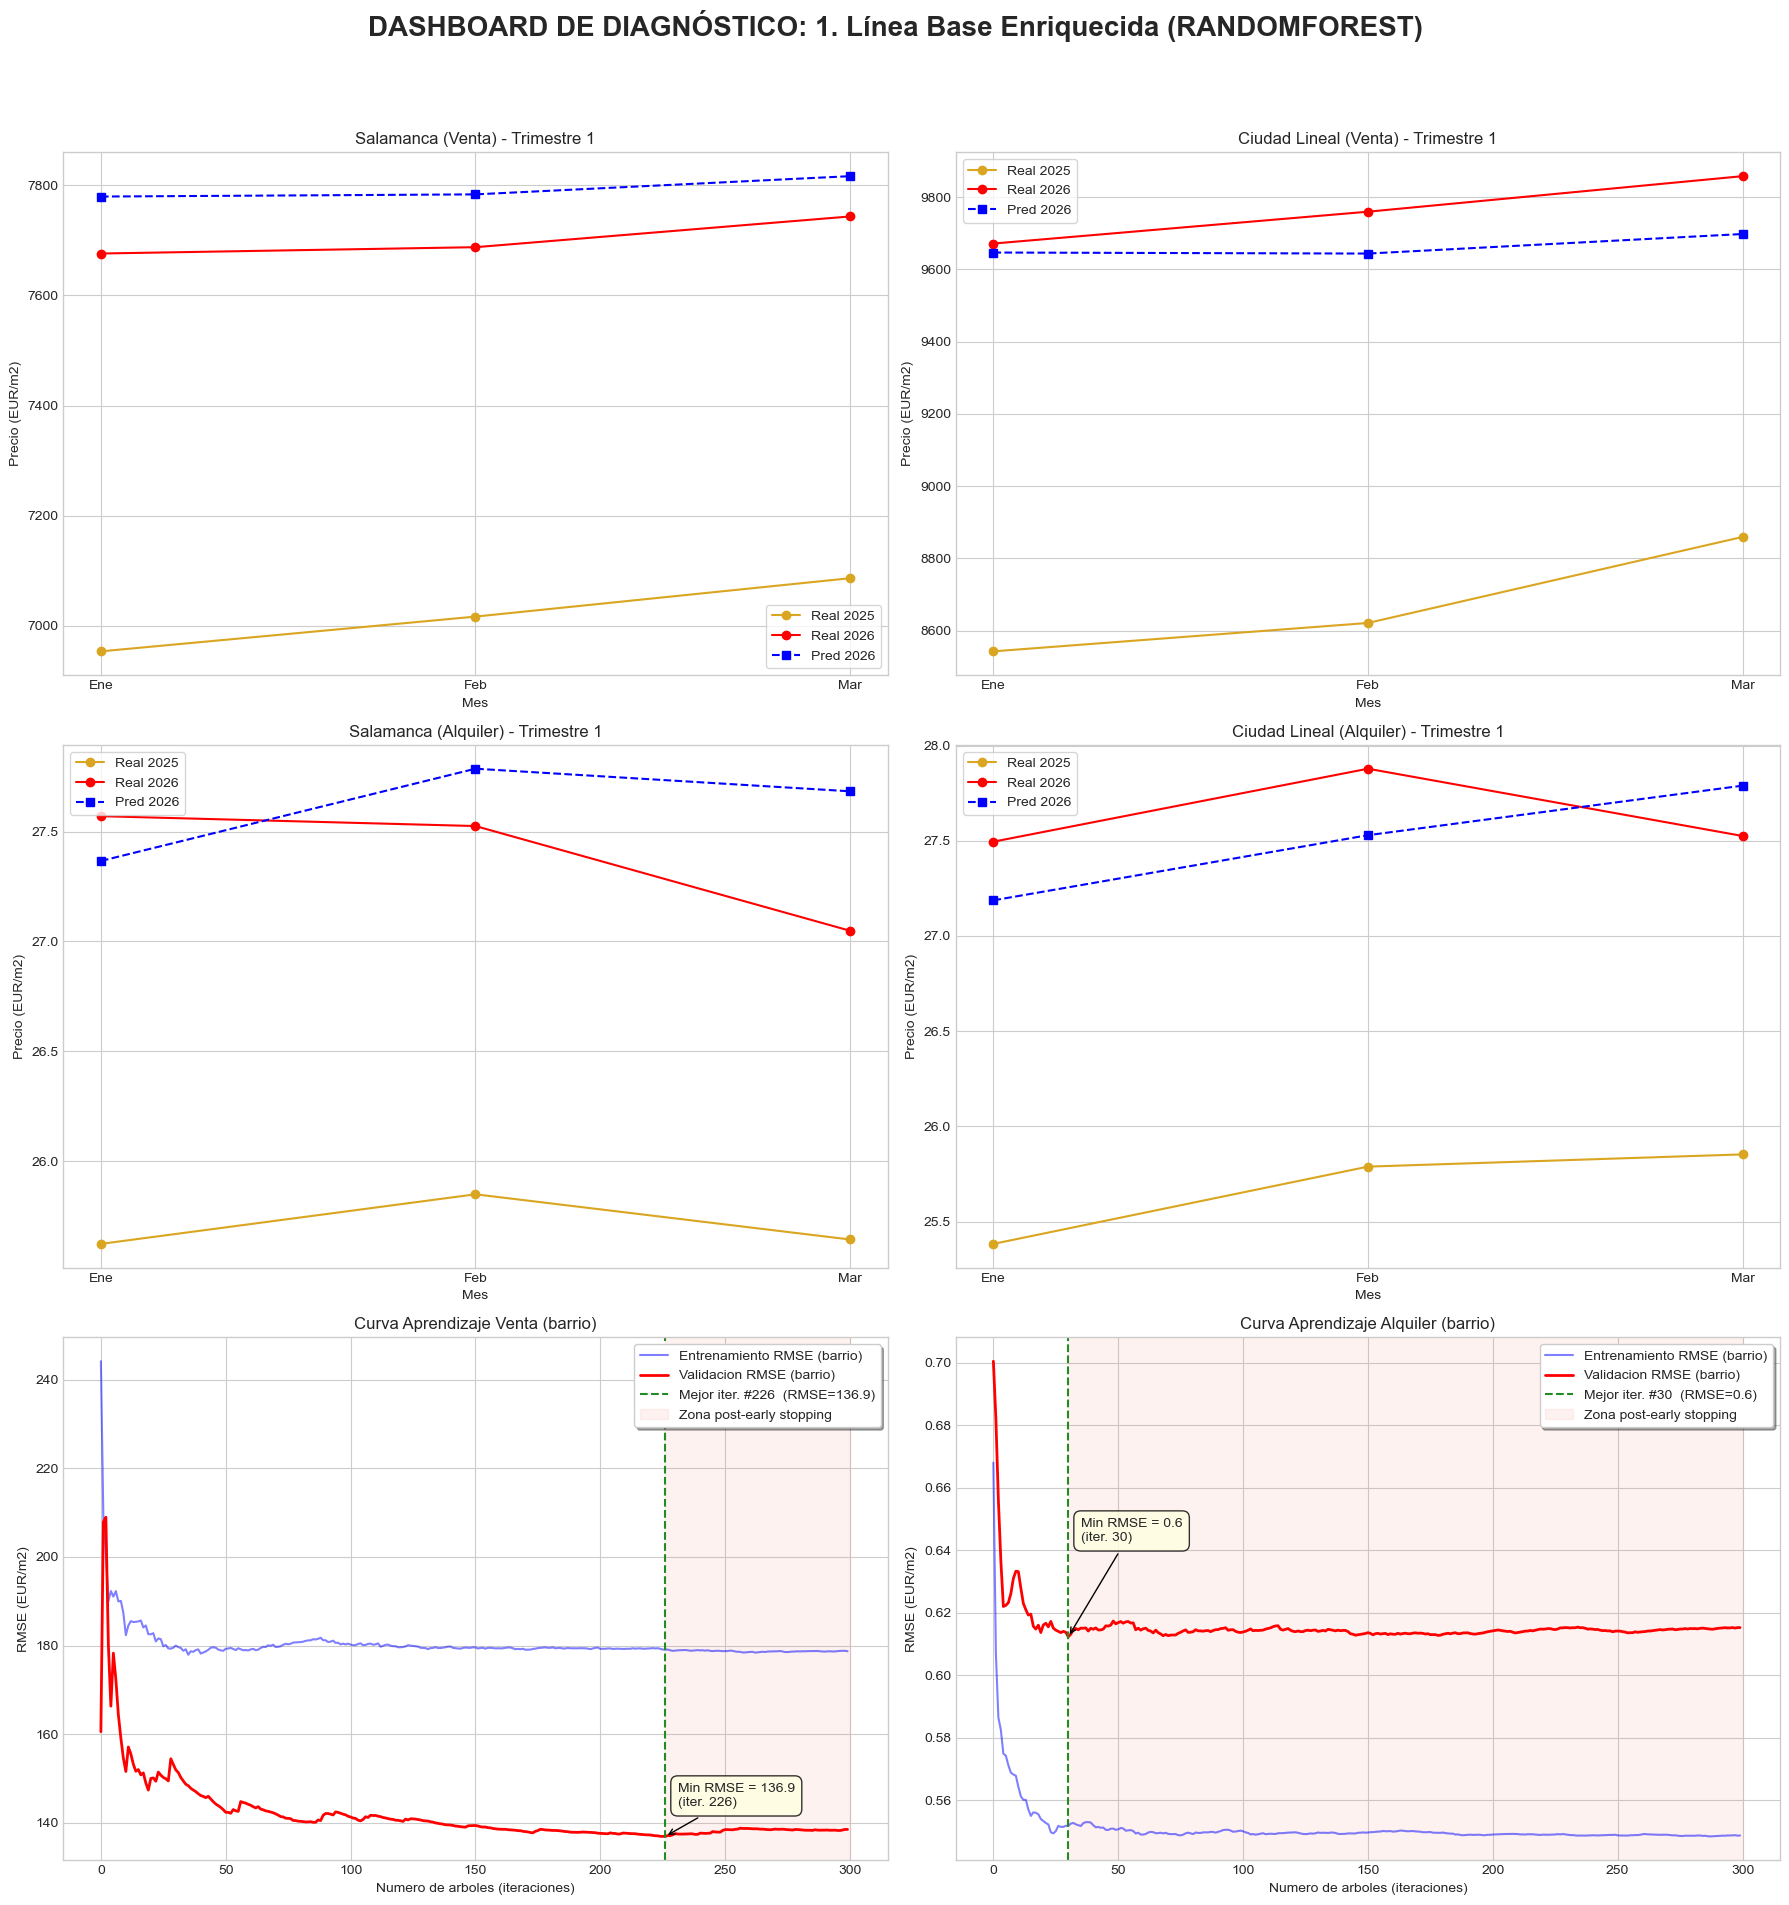
\includegraphics[width=1\linewidth]{img/fasea_randomforest.png}
\caption[Dashboard de la Fase A - Random Forest]{Dashboard de diagnóstico comparativo de la Fase A (Línea Base Enriquecida): Ajuste real vs. predicho y curva de aprendizaje de Random Forest.}
\label{fig:dashboard_fasea_rf}
\end{figure}

\begin{figure}[H]
\centering
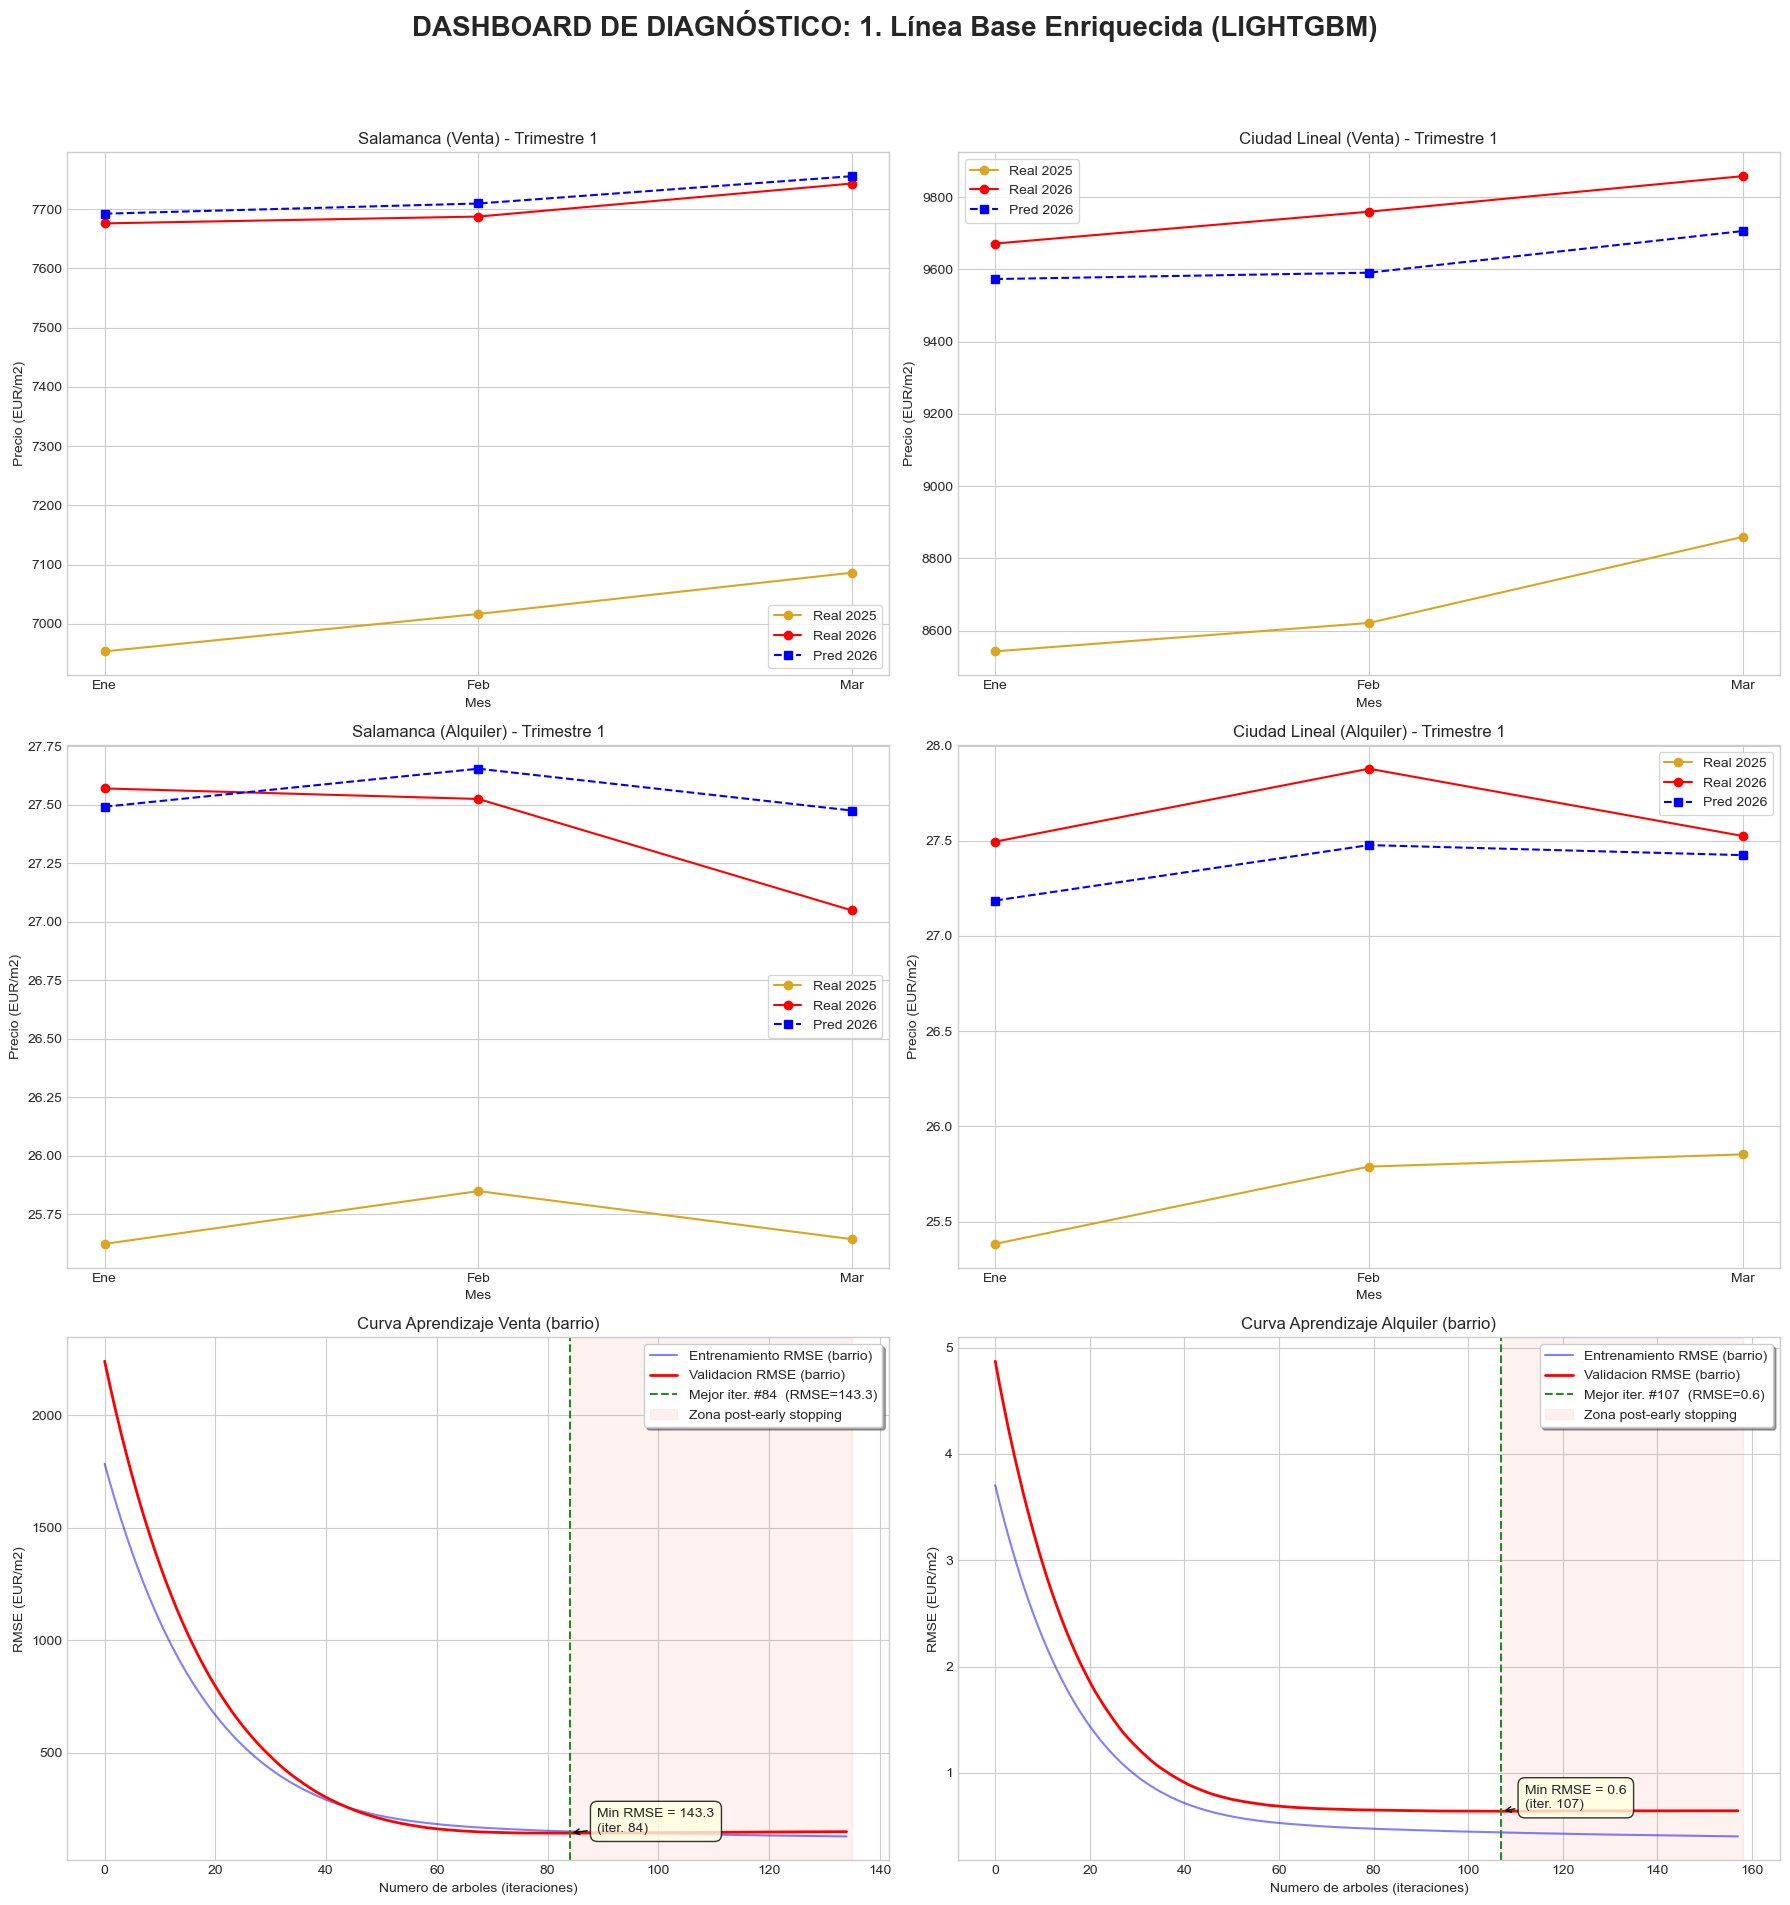
\includegraphics[width=1\linewidth]{img/fasea_lightgbm.png}
\caption[Dashboard de la Fase A - LightGBM]{Dashboard de diagnóstico comparativo de la Fase A (Línea Base Enriquecida): Ajuste real vs. predicho y curva de aprendizaje de LightGBM.}
\label{fig:dashboard_fasea_lgb}
\end{figure}

\begin{figure}[H]
\centering
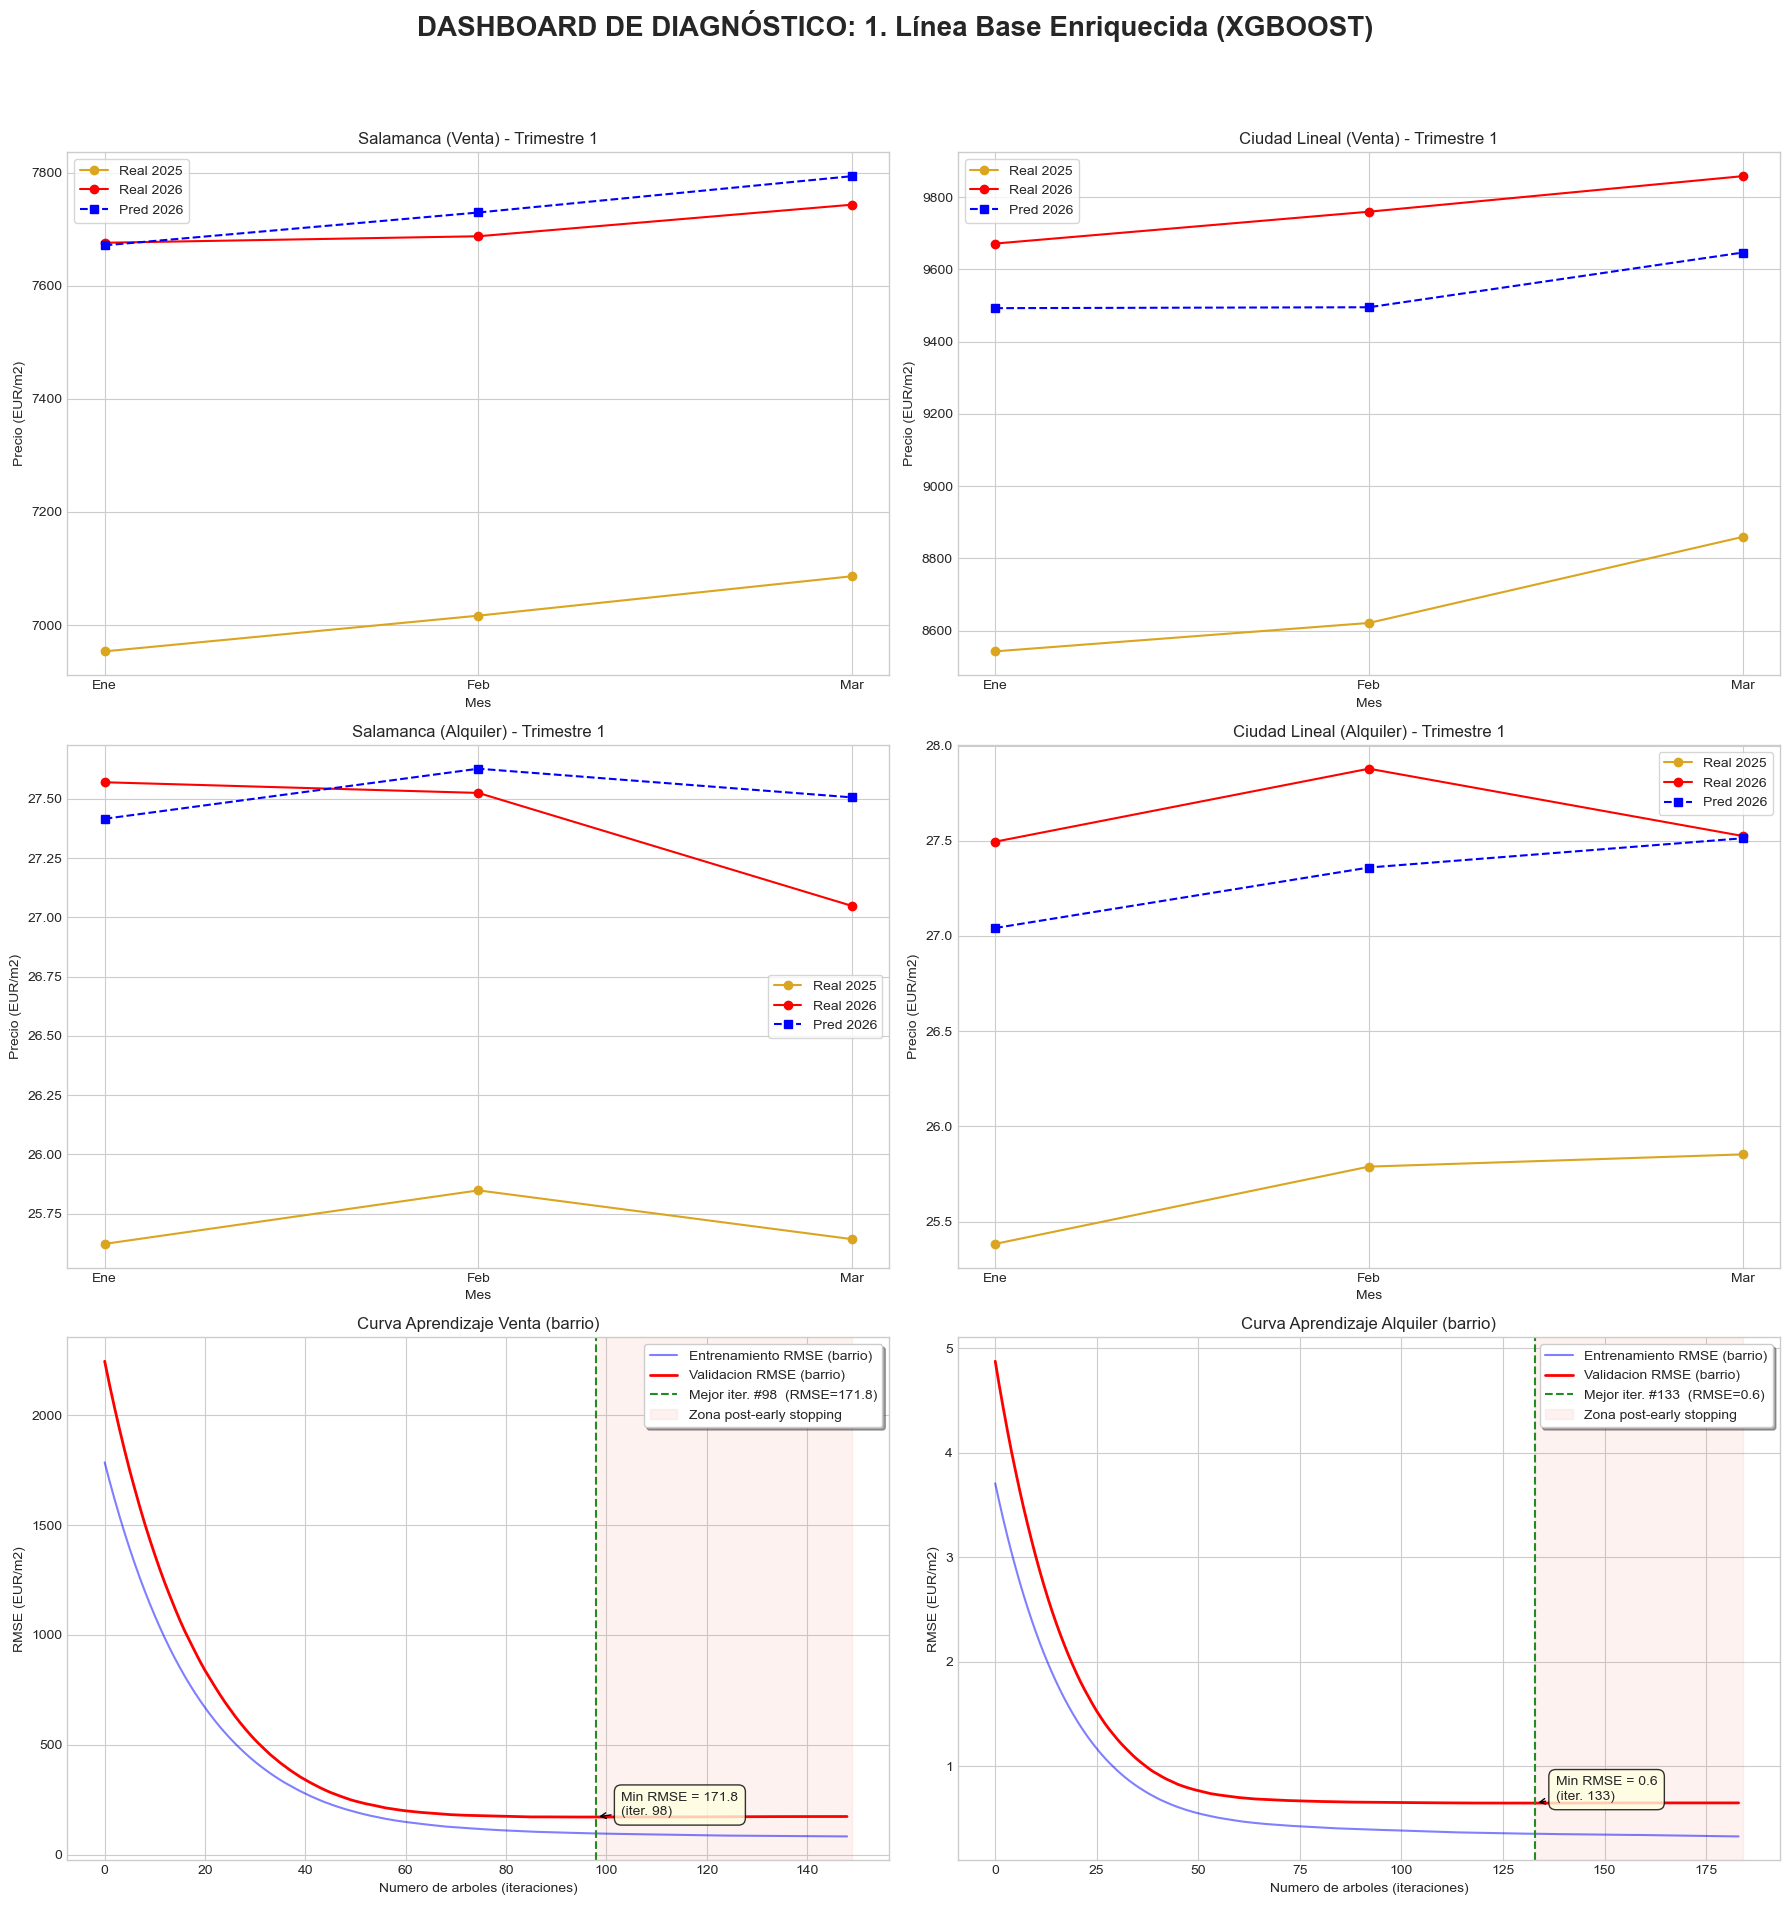
\includegraphics[width=1\linewidth]{img/fasea_xgboost.png}
\caption[Dashboard de la Fase A - XGBoost]{Dashboard de diagnóstico comparativo de la Fase A (Línea Base Enriquecida): Ajuste real vs. predicho y curva de aprendizaje de XGBoost.}
\label{fig:dashboard_fasea_xgb}
\end{figure}

\begin{figure}[H]
\centering
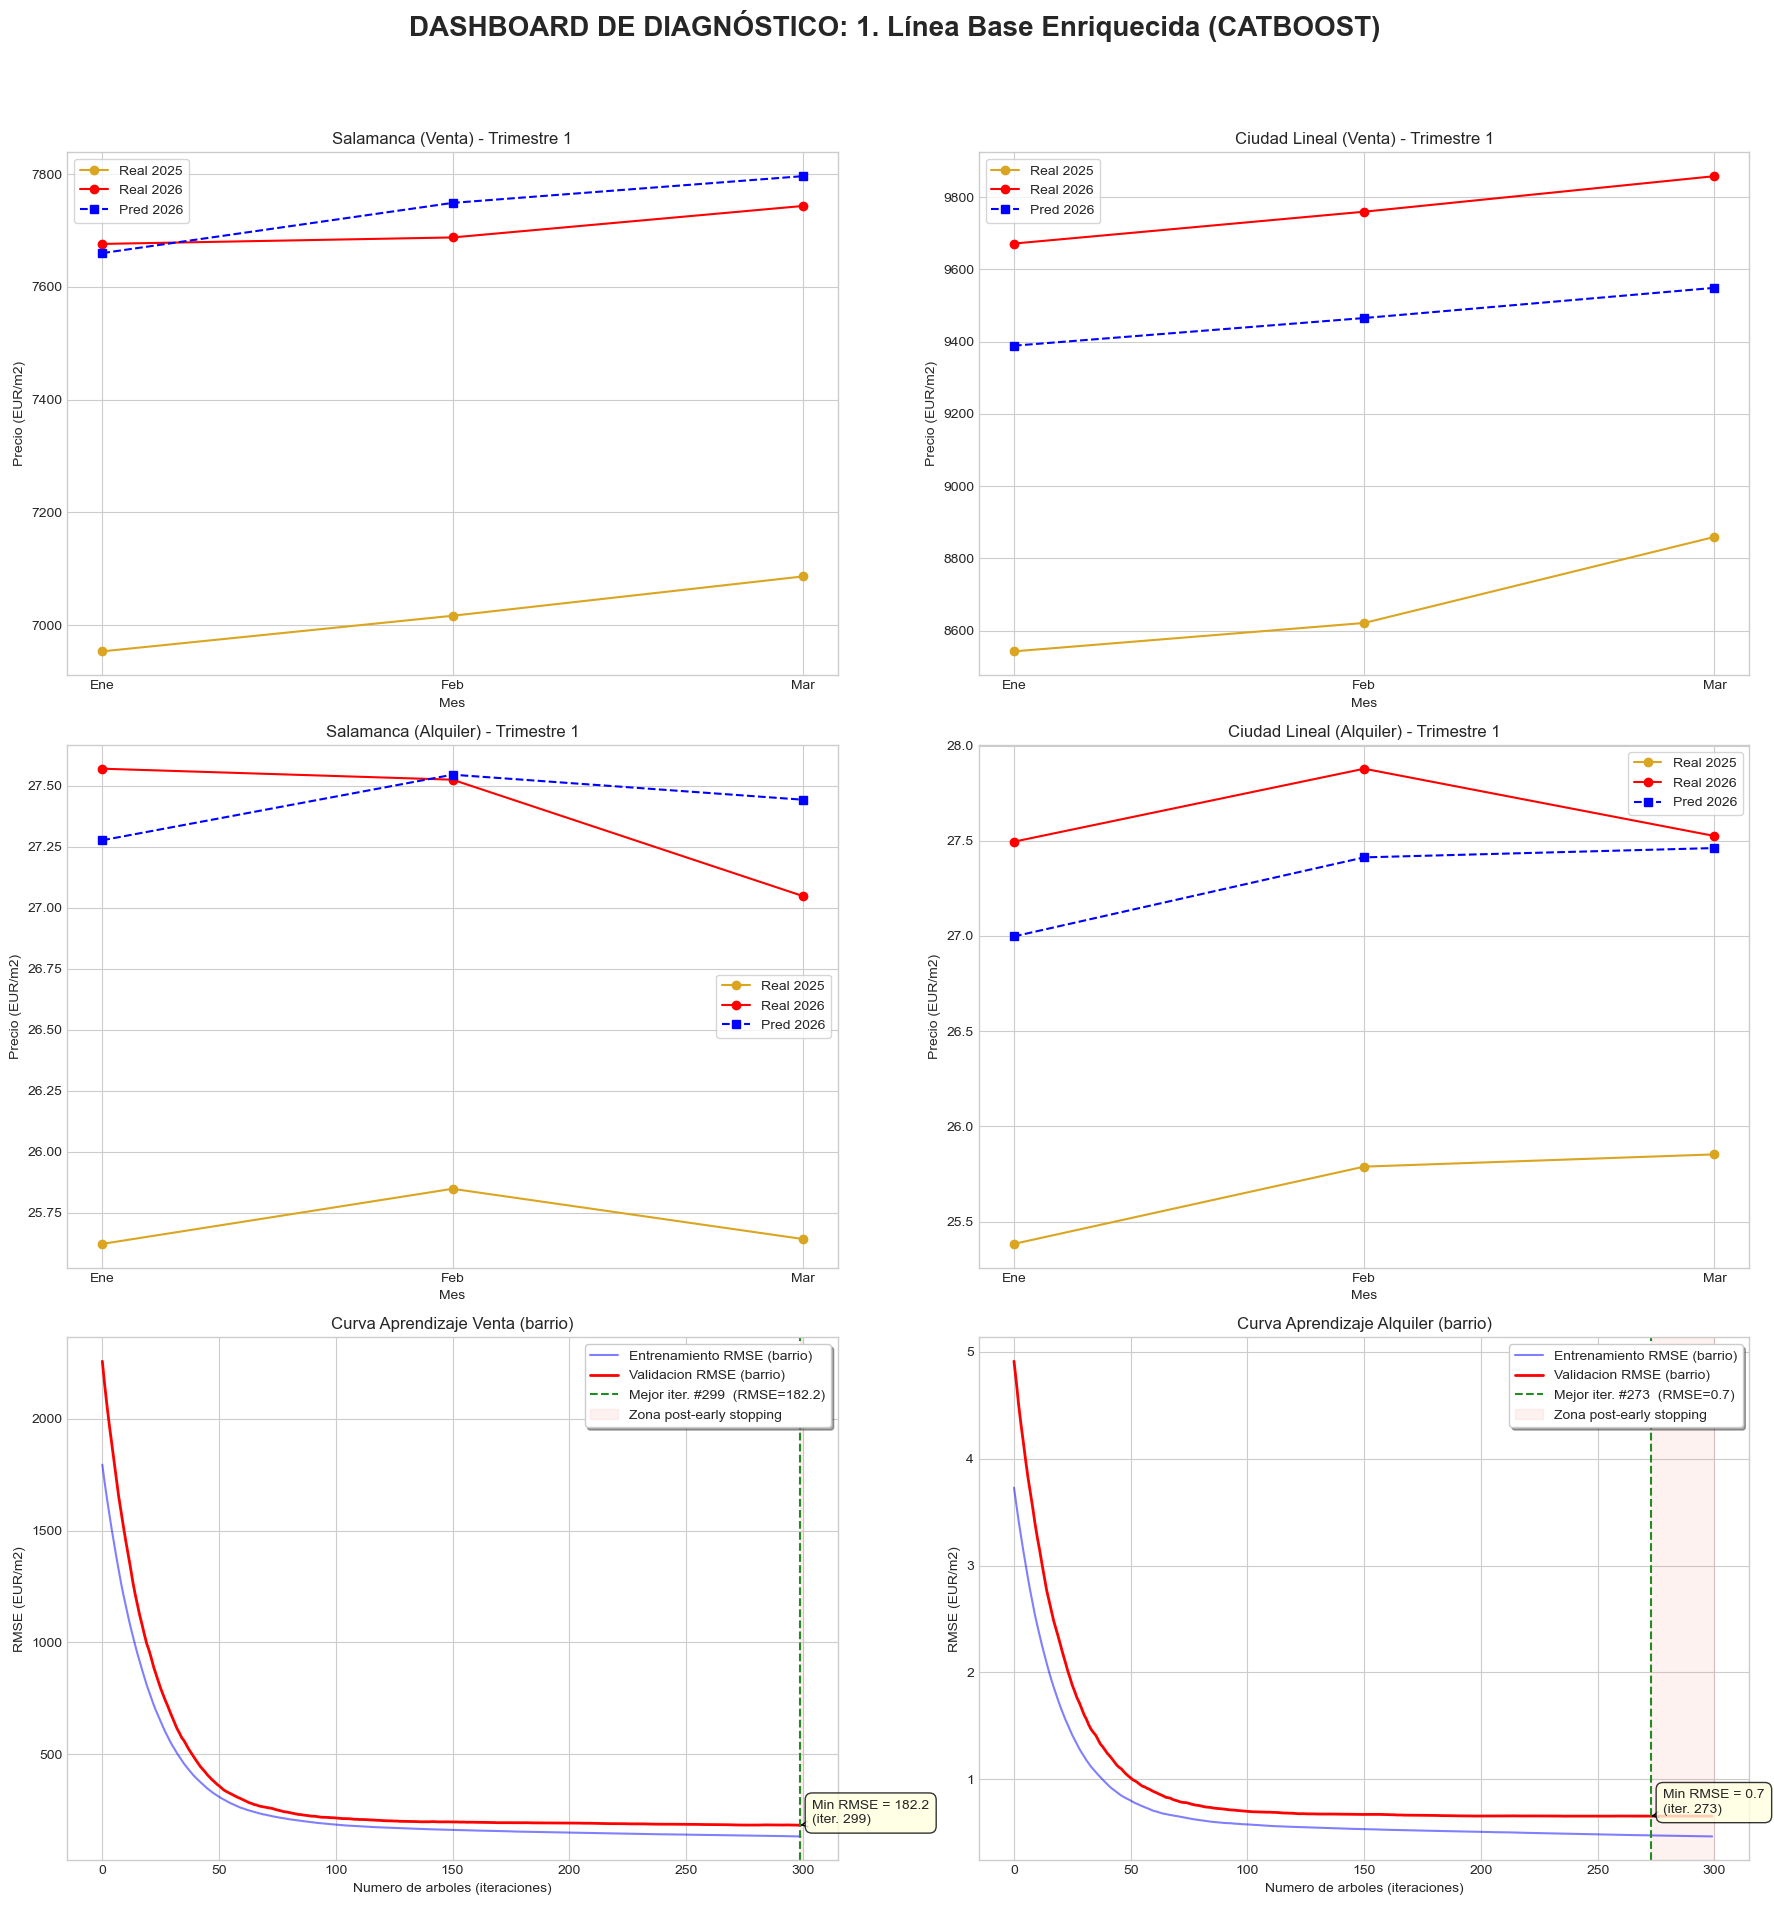
\includegraphics[width=1\linewidth]{img/fasea_catboost.png}
\caption[Dashboard de la Fase A - CatBoost]{Dashboard de diagnóstico comparativo de la Fase A (Línea Base Enriquecida): Ajuste real vs. predicho y curva de aprendizaje de CatBoost.}
\label{fig:dashboard_fasea_cat}
\end{figure}

Las figuras~\ref{fig:dashboard_fasea_rf}, \ref{fig:dashboard_fasea_lgb}, \ref{fig:dashboard_fasea_xgb} y \ref{fig:dashboard_fasea_cat} representan los dashboards de diagnóstico para los cuatro modelos. Cada dashboard muestra el ajuste entre el precio real (línea roja) y la predicción (línea azul) en 2026 (meses 1 a 3) junto a la referencia histórica de 2025 (línea dorada), y las curvas de aprendizaje asociadas:
\begin{itemize}
    \item \textbf{Random Forest (Figura~\ref{fig:dashboard_fasea_rf}):} En el mercado de venta para los distritos de Salamanca y Ciudad Lineal, las estimaciones muestran un comportamiento bastante satisfactorio y coherente. A nivel de venta global se obtiene un MAE de \textbf{99,97 €/m\textsuperscript{2}}; aunque en venta el modelo tiende a sobreestimar ligeramente los precios reales en Salamanca, la tendencia que sigue es muy precisa. En Ciudad Lineal (venta), las predicciones se sitúan ligeramente por debajo de los valores reales, mostrando un comportamiento más conservador o prudente, pero capturando de forma correcta los giros y ciclos del mercado. Por su parte, en el mercado de alquiler se observa una disparidad más marcada que en venta, con una leve tendencia a sobreestimar los precios de alquiler en Salamanca y a subestimarlos en Ciudad Lineal. Sus curvas de aprendizaje revelan una tendencia ruidosa: en venta la validación se sitúa atípicamente por debajo del entrenamiento (reflejando un ligero subajuste o \textit{underfitting} propio de la naturaleza del algoritmo y la distribución de los datos). Este comportamiento se justifica científicamente por dos factores:
    \begin{enumerate}
        \item \textit{Diferencia de Variabilidad y Varianza Temporal:} El conjunto de entrenamiento abarca tres años completos (2023, 2024, y 2025) a lo largo de todos los barrios de Madrid, lo cual introduce una enorme varianza espacial (precios muy heterogéneos) y temporal, con una desviación estándar muy alta. En cambio, el conjunto de validación de 2026 solo contiene una ventana temporal muy estrecha (enero, febrero y marzo), resultando una muestra mucho más homogénea que reduce la dispersión absoluta de los errores y hace que el RMSE (medido en valor absoluto de euros por metro cuadrado) sea matemáticamente menor.
        \item \textit{Limitaciones del Ajuste de Random Forest:} Al limitar la profundidad máxima de los árboles (\texttt{max\_depth=6}), el modelo está fuertemente regularizado. Dado que un Random Forest predice promediando estimadores independientes, su capacidad de sobreajustar al conjunto de entrenamiento está sumamente controlada; al enfrentarse a una ventana de test más acotada y de comportamiento más estable en 2026, el error absoluto resulta ser más bajo que el error promedio a lo largo de los tres años de entrenamiento.
    \end{enumerate}
    Por otro lado, en alquiler la validación se mantiene por encima del entrenamiento con una brecha mínima (entre \textbf{0,01 €/m\textsuperscript{2}} y \textbf{0,09 €/m\textsuperscript{2}}).
    \item \textbf{LightGBM (Figura~\ref{fig:dashboard_fasea_lgb}):} En comparación con Random Forest, este algoritmo ofrece un rendimiento muy superior y de alta precisión:
    \begin{itemize}
        \item \textit{Ajuste en Venta:} La precisión del modelo en venta es casi milimétrica en Salamanca en comparación con Random Forest; aunque persiste una mínima sobreestimación de los precios, representa la proyección más ajustada y real. En Ciudad Lineal (venta), la tendencia del modelo reproduce con éxito los patrones reales de manera muy similar a Random Forest.
        \item \textit{Ajuste en Alquiler:} La tendencia general es muy sólida, destacando su capacidad de generalización en Ciudad Lineal. Resuelve con éxito el problema observado en Random Forest, que sobreestimaba de forma atípica la caída de precios del mes de marzo de 2026; LightGBM no incurre en este sesgo, logrando una predicción muy cercana al valor real. En Salamanca (alquiler), la predicción resulta asimismo muy precisa.
        \item \textit{Curvas de Aprendizaje:} En venta, el RMSE de validación empieza a descender notablemente entre las iteraciones 20 y 40, alcanzando su mínimo absoluto en el rango de 60 a 80 (identificada la iteración 80 como la óptima, donde se observa un levísimo subajuste temporal antes de ascender de nuevo en la fase posterior al early stopping). En alquiler, las curvas muestran la mejor convergencia de todo el estudio: entrenamiento y validación se acoplan perfectamente sin mostrar signos de subajuste ni sobreajuste, alcanzando el óptimo en el árbol 107 (frente al 30 de Random Forest), demostrando una mayor asimilación de patrones complejos con un RMSE final de \textbf{0,6 €/m\textsuperscript{2}}.
    \end{itemize}
    \item \textbf{XGBoost (Figura~\ref{fig:dashboard_fasea_xgb}):} Este algoritmo presenta un comportamiento sumamente competitivo, consolidando la superioridad de las técnicas de boosting frente a bagging:
    \begin{itemize}
        \item \textit{Ajuste en Venta:} Sigue una tendencia similar a LightGBM, manifestando una inclinación a sobreestimar los precios en Salamanca y mostrándose más conservador en Ciudad Lineal. Aunque su ajuste no es tan milimétrico como el de LightGBM, su comportamiento es muy robusto.
        \item \textit{Ajuste en Alquiler:} La tendencia coincide casi plenamente con la de LightGBM. Sin embargo, XGBoost demuestra ser aún más preciso en Ciudad Lineal en la predicción del mes de marzo de 2026, acoplándose con gran exactitud a la realidad. Las tendencias limpias confirman que los modelos de gradiente de boosting generalizan de manera muy superior y eliminan los problemas de ajuste local de Random Forest.
        \item \textit{Curvas de Aprendizaje:} A diferencia de los otros modelos, en XGBoost la línea de validación se mantiene de forma consistente por encima de la de entrenamiento en todo momento, confirmando la \textbf{ausencia absoluta de subajuste (\textit{underfitting})}. En venta, alcanza su mejor iteración en el árbol 98 (con un RMSE de \textbf{171,81 €/m\textsuperscript{2}}). En alquiler, la mejor iteración se dilata hasta el árbol 133 (en comparación con 107 en LightGBM y 30 en Random Forest), indicando que el algoritmo prolonga su capacidad de aprendizaje antes de alcanzar el error óptimo de validación, registrando un RMSE de \textbf{0,64 €/m\textsuperscript{2}}.
    \end{itemize}
    \item \textbf{CatBoost (Figura~\ref{fig:dashboard_fasea_cat}):} El último de los algoritmos de gradiente de boosting evaluados ofrece un comportamiento muy interesante en términos de generalización:
    \begin{itemize}
        \item \textit{Ajuste en Venta:} Sigue el patrón general de sobreestimar los precios en Salamanca y mostrar una postura más conservadora en Ciudad Lineal. En Ciudad Lineal, a pesar de que la tendencia del ajuste es notablemente limpia y se acopla bien a la realidad, presenta un error absoluto (MAE de \textbf{327,28 €/m\textsuperscript{2}}) ligeramente superior al resto de modelos.
        \item \textit{Ajuste en Alquiler:} Las curvas reales y predichas siguen tendencias muy limpias y consistentes. En Salamanca, el error mínimo (MAE de \textbf{0,4761 €/m\textsuperscript{2}}) es muy similar al de los otros boostings, aunque ligeramente superior (aproximadamente 0,1 €/m\textsuperscript{2} más que XGBoost y LightGBM). En Ciudad Lineal, el MAE se sitúa en \textbf{0,7126 €/m\textsuperscript{2}}.
        \item \textit{Curvas de Aprendizaje:} Muestra una convergencia sumamente limpia, donde la curva de validación se acopla casi por completo a la de entrenamiento sin mostrar signos de sobreajuste ni subajuste. El mejor punto se alcanza en la iteración 173, lo que indica que CatBoost dilata más su entrenamiento y requiere un mayor número de árboles para aprender las relaciones complejas y regularizar sus predicciones antes de estabilizarse.
    \end{itemize}
\end{itemize}

El análisis comparativo detallado de la Fase A ayuda a establecer un veredicto definitivo sobre los modelos:
\begin{itemize}
    \item \textbf{Para el Mercado de Venta:} XGBoost y LightGBM destacan como las mejores alternativas debido a su menor error y su capacidad de aprendizaje. Random Forest queda penalizado por su tendencia al subajuste ruidoso y CatBoost se sitúa en tercera posición debido a un error absoluto algo mayor. En este mercado, \textbf{XGBoost destaca como superior} por registrar el menor sesgo global del estudio (\textbf{-4,69 €/m\textsuperscript{2}} frente a los \textbf{13,23 €/m\textsuperscript{2}} de LightGBM y los sesgos más elevados de los otros modelos).
    \item \textbf{Para el Mercado de Alquiler:} \textbf{LightGBM destaca como el mejor modelo} por presentar el menor error absoluto global y el sesgo más cercano a cero (\textbf{-0,0262 €/m\textsuperscript{2}} frente a los \textbf{-0,0508 €/m\textsuperscript{2}} de XGBoost y \textbf{-0,0852 €/m\textsuperscript{2}} de CatBoost). XGBoost y CatBoost ocupan una segunda posición muy competitiva, mientras que Random Forest queda rezagado debido a los problemas de generalización local descritos en el mes de marzo en Ciudad Lineal.
\end{itemize}



\subsection{Fase B: Optimización de la Inercia Temporal (Tratamiento de Shocks)}
El mayor reto identificado durante el análisis de 2025--2026 fue la inercia temporal. El mercado inmobiliario madrileño experimentó una aceleración alcista atípica durante 2025. Los algoritmos tradicionales de gradiente de boosting (como XGBoost o LightGBM) sufren para capturar este comportamiento si operan únicamente con retardos clásicos, con lo que sus predicciones regresan a los niveles de 2024 y subestiman sistemáticamente los precios reales de 2026.

Este fenómeno de deriva de conceptos y desplazamiento de distribución (\textit{Concept Drift} y \textit{Distribution Shift}) ha sido ampliamente estudiado en la literatura de series temporales. En el ámbito del aprendizaje automático, una estrategia fundamental es la ponderación de muestras basada en el tiempo (\textit{temporal sample weighting} o \textit{time-based forgetting}). Como demostró Koychev (2004) en su paper clásico \textit{``Gradual Forgetting for Adaptation to Concept Drift''}, la relevancia de los ejemplos de entrenamiento disminuye con el tiempo, por lo que es necesario asignar un peso mayor a las observaciones recientes frente a las antiguas mediante funciones de decaimiento. Recientemente, Bennett y Clarkson (2025) en \textit{``Time Series Prediction under Distribution Shift using Differentiable Forgetting''} formalizan este enfoque como un problema de minimización del riesgo empírico ponderado (\textit{Weighted Empirical Risk Minimization}), donde el mecanismo de olvido regula el balance entre la relevancia del concepto actual y el tamaño efectivo de la muestra. Para modelos de ensamble como Random Forest, el uso de funciones de decaimiento temporal facilitan ponderar de forma óptima la influencia de muestras antiguas al aprender nuevos árboles (Ikonomovska et al., 2016). Asimismo, en algoritmos de Gradient Boosting, la inyección de esquemas de ponderación basados en la inercia temporal ayuda a mitigar la inercia estocástica y favorecer el aprendizaje de tendencias alcistas bruscas sin incurrir en un sobreajuste severo del modelo (Jiang et al., 2020).

Para comprender la magnitud de la perturbación estacional ocurrida en Madrid, la Tabla~\ref{tab:patrones_estacionales} sistematiza la evolución mensual y anual observada en los mercados de venta y alquiler durante el periodo bajo estudio (2023--2026 Q1), lo que refleja cómo la estacionalidad clásica se rompió abruptamente en 2025 hacia un comportamiento de crecimiento continuo e ininterrumpido (Cisne Negro).

\begin{table}[H]
\centering
\resizebox{\textwidth}{!}{%
\begin{tabular}{|l|c|c|c|c|c|c|c|c|c|c|c|c|}
\hline
\textbf{Año / Operación} & \textbf{Ene} & \textbf{Feb} & \textbf{Mar} & \textbf{Abr} & \textbf{May} & \textbf{Jun} & \textbf{Jul} & \textbf{Ago} & \textbf{Sep} & \textbf{Oct} & \textbf{Nov} & \textbf{Dic} \\
\hline
\multicolumn{13}{|l|}{\textbf{MERCADO DE VENTA (Patrón Mensual por Año)}} \\
\hline
\textbf{2023 (Ciclo clásico)} & $\rightarrow$ & $\uparrow$ & $\uparrow\uparrow$ & $\uparrow\uparrow$ & $\uparrow$ & $\rightarrow$ & $\downarrow$ & $\downarrow$ & $\rightarrow$ & $\uparrow$ & $\rightarrow$ & $\downarrow$ \\
\textbf{2024 (Aceleración)} & $\rightarrow$ & $\uparrow$ & $\uparrow\uparrow$ & $\uparrow\uparrow$ & $\uparrow$ & $\uparrow$ & $\rightarrow$ & $\downarrow$ & $\rightarrow$ & $\uparrow$ & $\uparrow$ & $\rightarrow$ \\
\textbf{2025 (Cisne Negro)} & $\uparrow$ & $\uparrow\uparrow$ & $\uparrow\uparrow$ & $\uparrow\uparrow$ & $\uparrow\uparrow$ & $\uparrow\uparrow$ & $\uparrow$ & $\uparrow$ & $\uparrow$ & $\uparrow\uparrow$ & $\uparrow\uparrow\uparrow$ & $\uparrow\uparrow$ \\
\textbf{2026 Q1 (Datos reales)} & 5.480€ & 5.521€ & 5.548€ & -- & -- & -- & -- & -- & -- & -- & -- & -- \\
\hline
\multicolumn{13}{|l|}{\textbf{MERCADO DE ALQUILER (Patrón Mensual por Año)}} \\
\hline
\textbf{2023 (Estac. clásica)} & $\downarrow\downarrow$ & $\downarrow$ & $\rightarrow$ & $\rightarrow$ & $\uparrow$ & $\uparrow$ & $\uparrow\uparrow$ & $\uparrow\uparrow$ & $\uparrow\uparrow\uparrow$ & $\rightarrow$ & $\downarrow$ & $\downarrow$ \\
\textbf{2024 (Presión creciente)} & $\downarrow$ & $\rightarrow$ & $\rightarrow$ & $\uparrow$ & $\uparrow$ & $\uparrow$ & $\uparrow\uparrow$ & $\uparrow\uparrow$ & $\uparrow\uparrow\uparrow$ & $\uparrow$ & $\rightarrow$ & $\downarrow$ \\
\textbf{2025 (Estac. amplificada)} & $\uparrow$ & $\uparrow$ & $\uparrow\uparrow$ & $\uparrow\uparrow$ & $\uparrow\uparrow$ & $\uparrow\uparrow$ & $\uparrow\uparrow$ & $\uparrow\uparrow$ & $\uparrow\uparrow\uparrow$ & $\uparrow\uparrow$ & $\uparrow\uparrow$ & $\uparrow\uparrow\uparrow$ \\
\textbf{2026 Q1 (Máximos)} & 21.2€ & Máx & Máx & -- & -- & -- & -- & -- & -- & -- & -- & -- \\
\hline
\end{tabular}%
}
\caption{Matriz de evolución intermensual de precios inmobiliarios en Madrid (2023--2026 Q1) detallando la transición hacia la estacionalidad resiliente ($\downarrow\downarrow$ Bajada fuerte, $\downarrow$ Bajada, $\rightarrow$ Estable, $\uparrow$ Subida leve, $\uparrow\uparrow$ Subida moderada, $\uparrow\uparrow\uparrow$ Subida fuerte).}
\label{tab:patrones_estacionales}
\end{table}

Para modelar este shock, se contrastaron dos tratamientos paramétricos de ponderación temporal de muestras (\textit{Sample Weights}) frente a la \textbf{Línea de Control} (Fase A - sin ponderar).

\subsubsection{Experimento 1: Shock Agresivo (Peso Estático 3.0)}
Este tratamiento asigna un peso constante y agresivo de 3.0 a todas las muestras del año 2025 en el entrenamiento, con el propósito de forzar a los algoritmos a priorizar el comportamiento alcista reciente de la serie temporal. Las métricas resultantes se exponen de forma detallada en la Tabla~\ref{tab:fase_b_exp1_venta} para el mercado de venta y en la Tabla~\ref{tab:fase_b_exp1_alquiler} para el mercado de alquiler.

\begin{table}[H]
\centering
\resizebox{\textwidth}{!}{%
\begin{tabular}{|l|c|c|c|c|c|c|c|c|c|}
\hline
\textbf{Algoritmo} & \textbf{MAE Global} & \textbf{RMSE Global} & \textbf{R\textsuperscript{2} Global} & \textbf{MAE Salam.} & \textbf{R\textsuperscript{2} Salam.} & \textbf{MAE C. Lineal} & \textbf{R\textsuperscript{2} C. Lineal} & \textbf{T. Train (s)} & \textbf{T. Pred (s)} \\
 & \textbf{(€/m\textsuperscript{2})} & \textbf{(€/m\textsuperscript{2})} & & \textbf{(€/m\textsuperscript{2})} & & \textbf{(€/m\textsuperscript{2})} & & & \\
\hline
\textbf{Random Forest} & 100,19 & 135,85 & 0,9957 & 118,73 & 0,9700 & 145,89 & 0,9860 & 1,2068 & 0,0397 \\
\textbf{LightGBM} & 102,47 & 139,11 & 0,9955 & 77,19 & 0,9797 & 193,10 & 0,9725 & 0,1533 & 0,0034 \\
\textbf{XGBoost} & 112,34 & 151,68 & 0,9946 & 92,42 & 0,9703 & 159,26 & 0,9835 & 0,3415 & 0,0050 \\
\textbf{CatBoost} & 126,85 & 178,30 & 0,9926 & 111,79 & 0,9733 & 254,50 & 0,9556 & 1,1439 & 0,0014 \\
\hline
\end{tabular}%
}
\caption{Métricas obtenidas en el Mercado de Venta para el Experimento 1 (Shock Agresivo con Peso Estático 3.0 en 2025).}
\label{tab:fase_b_exp1_venta}
\end{table}

\begin{table}[H]
\centering
\resizebox{\textwidth}{!}{%
\begin{tabular}{|l|c|c|c|c|c|c|c|c|c|}
\hline
\textbf{Algoritmo} & \textbf{MAE Global} & \textbf{RMSE Global} & \textbf{R\textsuperscript{2} Global} & \textbf{MAE Salam.} & \textbf{R\textsuperscript{2} Salam.} & \textbf{MAE C. Lineal} & \textbf{R\textsuperscript{2} C. Lineal} & \textbf{T. Train (s)} & \textbf{T. Pred (s)} \\
 & \textbf{(€/m\textsuperscript{2})} & \textbf{(€/m\textsuperscript{2})} & & \textbf{(€/m\textsuperscript{2})} & & \textbf{(€/m\textsuperscript{2})} & & & \\
\hline
\textbf{Random Forest} & 0,4658 & 0,6207 & 0,9743 & 0,4358 & 0,7756 & 0,5057 & 0,9693 & 1,0835 & 0,0409 \\
\textbf{LightGBM} & 0,4967 & 0,6543 & 0,9715 & 0,4349 & 0,8043 & 0,6477 & 0,9413 & 0,2479 & 0,0020 \\
\textbf{XGBoost} & 0,5074 & 0,6688 & 0,9702 & 0,5334 & 0,7161 & 0,7023 & 0,9288 & 0,3880 & 0,0040 \\
\textbf{CatBoost} & 0,5419 & 0,6887 & 0,9684 & 0,4962 & 0,7552 & 0,8317 & 0,9125 & 1,3467 & 0,0035 \\
\hline
\end{tabular}%
}
\caption{Métricas obtenidas en el Mercado de Alquiler para el Experimento 1 (Shock Agresivo con Peso Estático 3.0 en 2025).}
\label{tab:fase_b_exp1_alquiler}
\end{table}

Las figuras~\ref{fig:db_faseb_agresivo_rf}, \ref{fig:db_faseb_agresivo_lgb}, \ref{fig:db_faseb_agresivo_xgb} y \ref{fig:db_faseb_agresivo_cat} muestran los dashboards comparativos de ajuste y curvas de aprendizaje en el Experimento 1:

\begin{figure}[H]
\centering
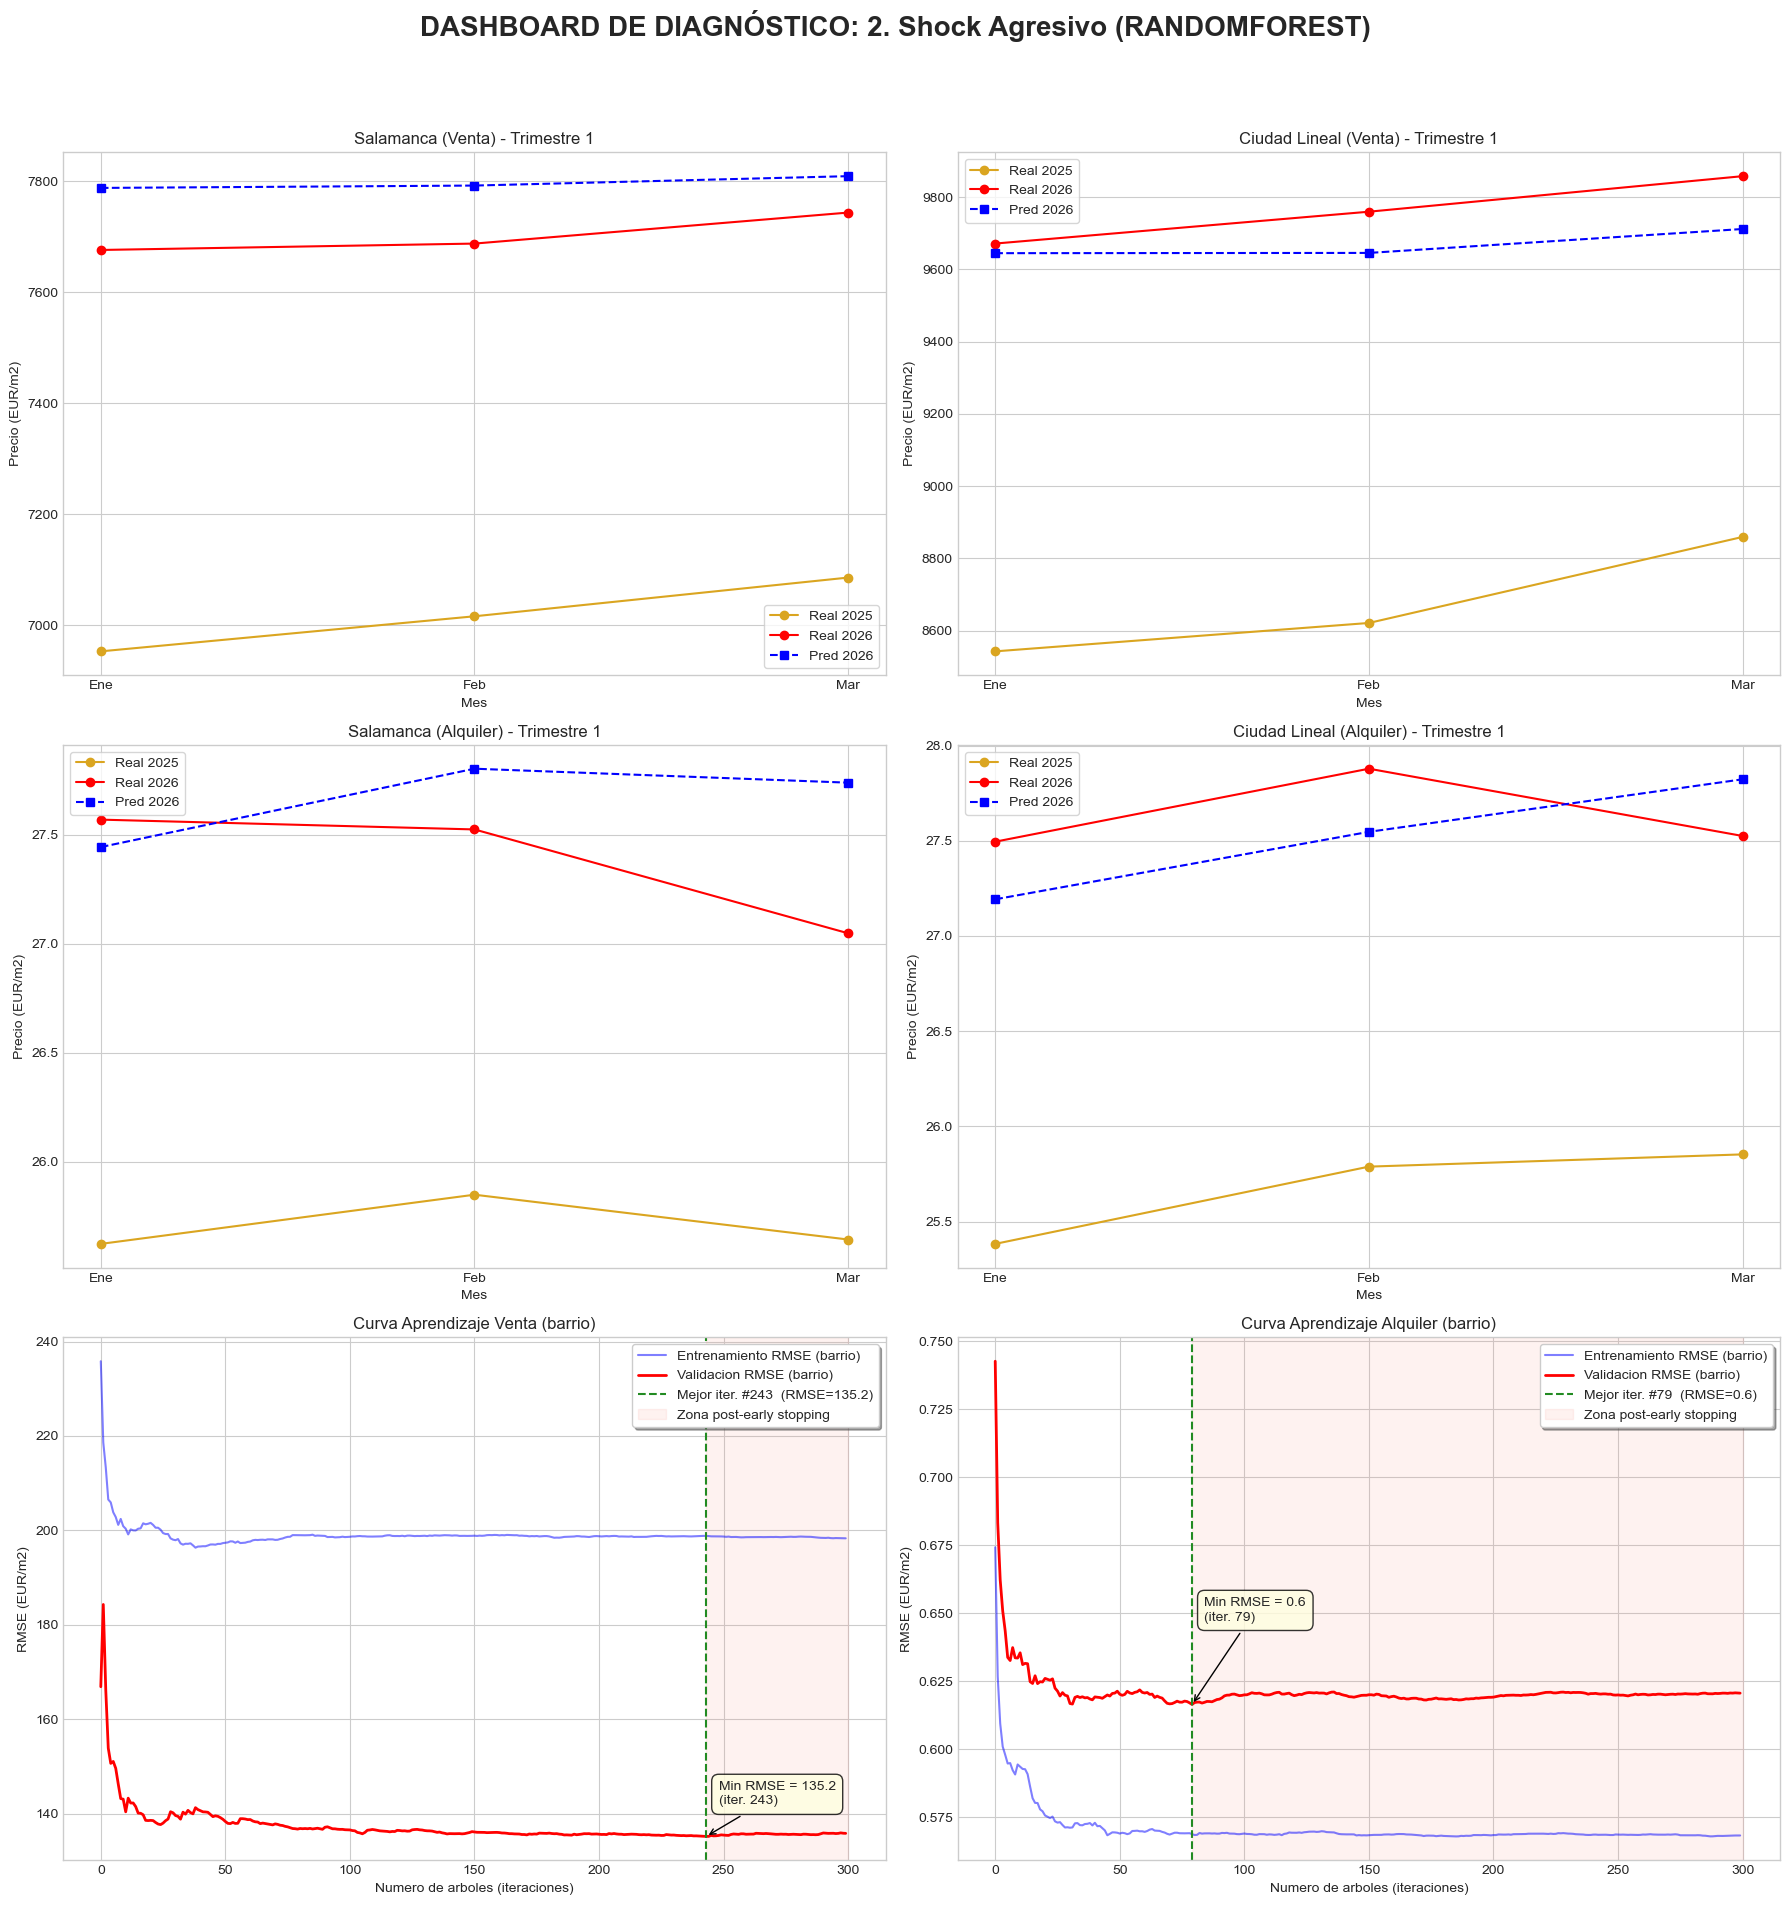
\includegraphics[width=1\linewidth]{img/faseb_agresivo_RandomForest.png}
\caption[Dashboard del Experimento 1 (Shock Agresivo) - Random Forest]{Dashboard comparativo del Experimento 1 (Shock Agresivo): Ajuste real vs. predicho y curva de aprendizaje para Random Forest.}
\label{fig:db_faseb_agresivo_rf}
\end{figure}

\begin{figure}[H]
\centering
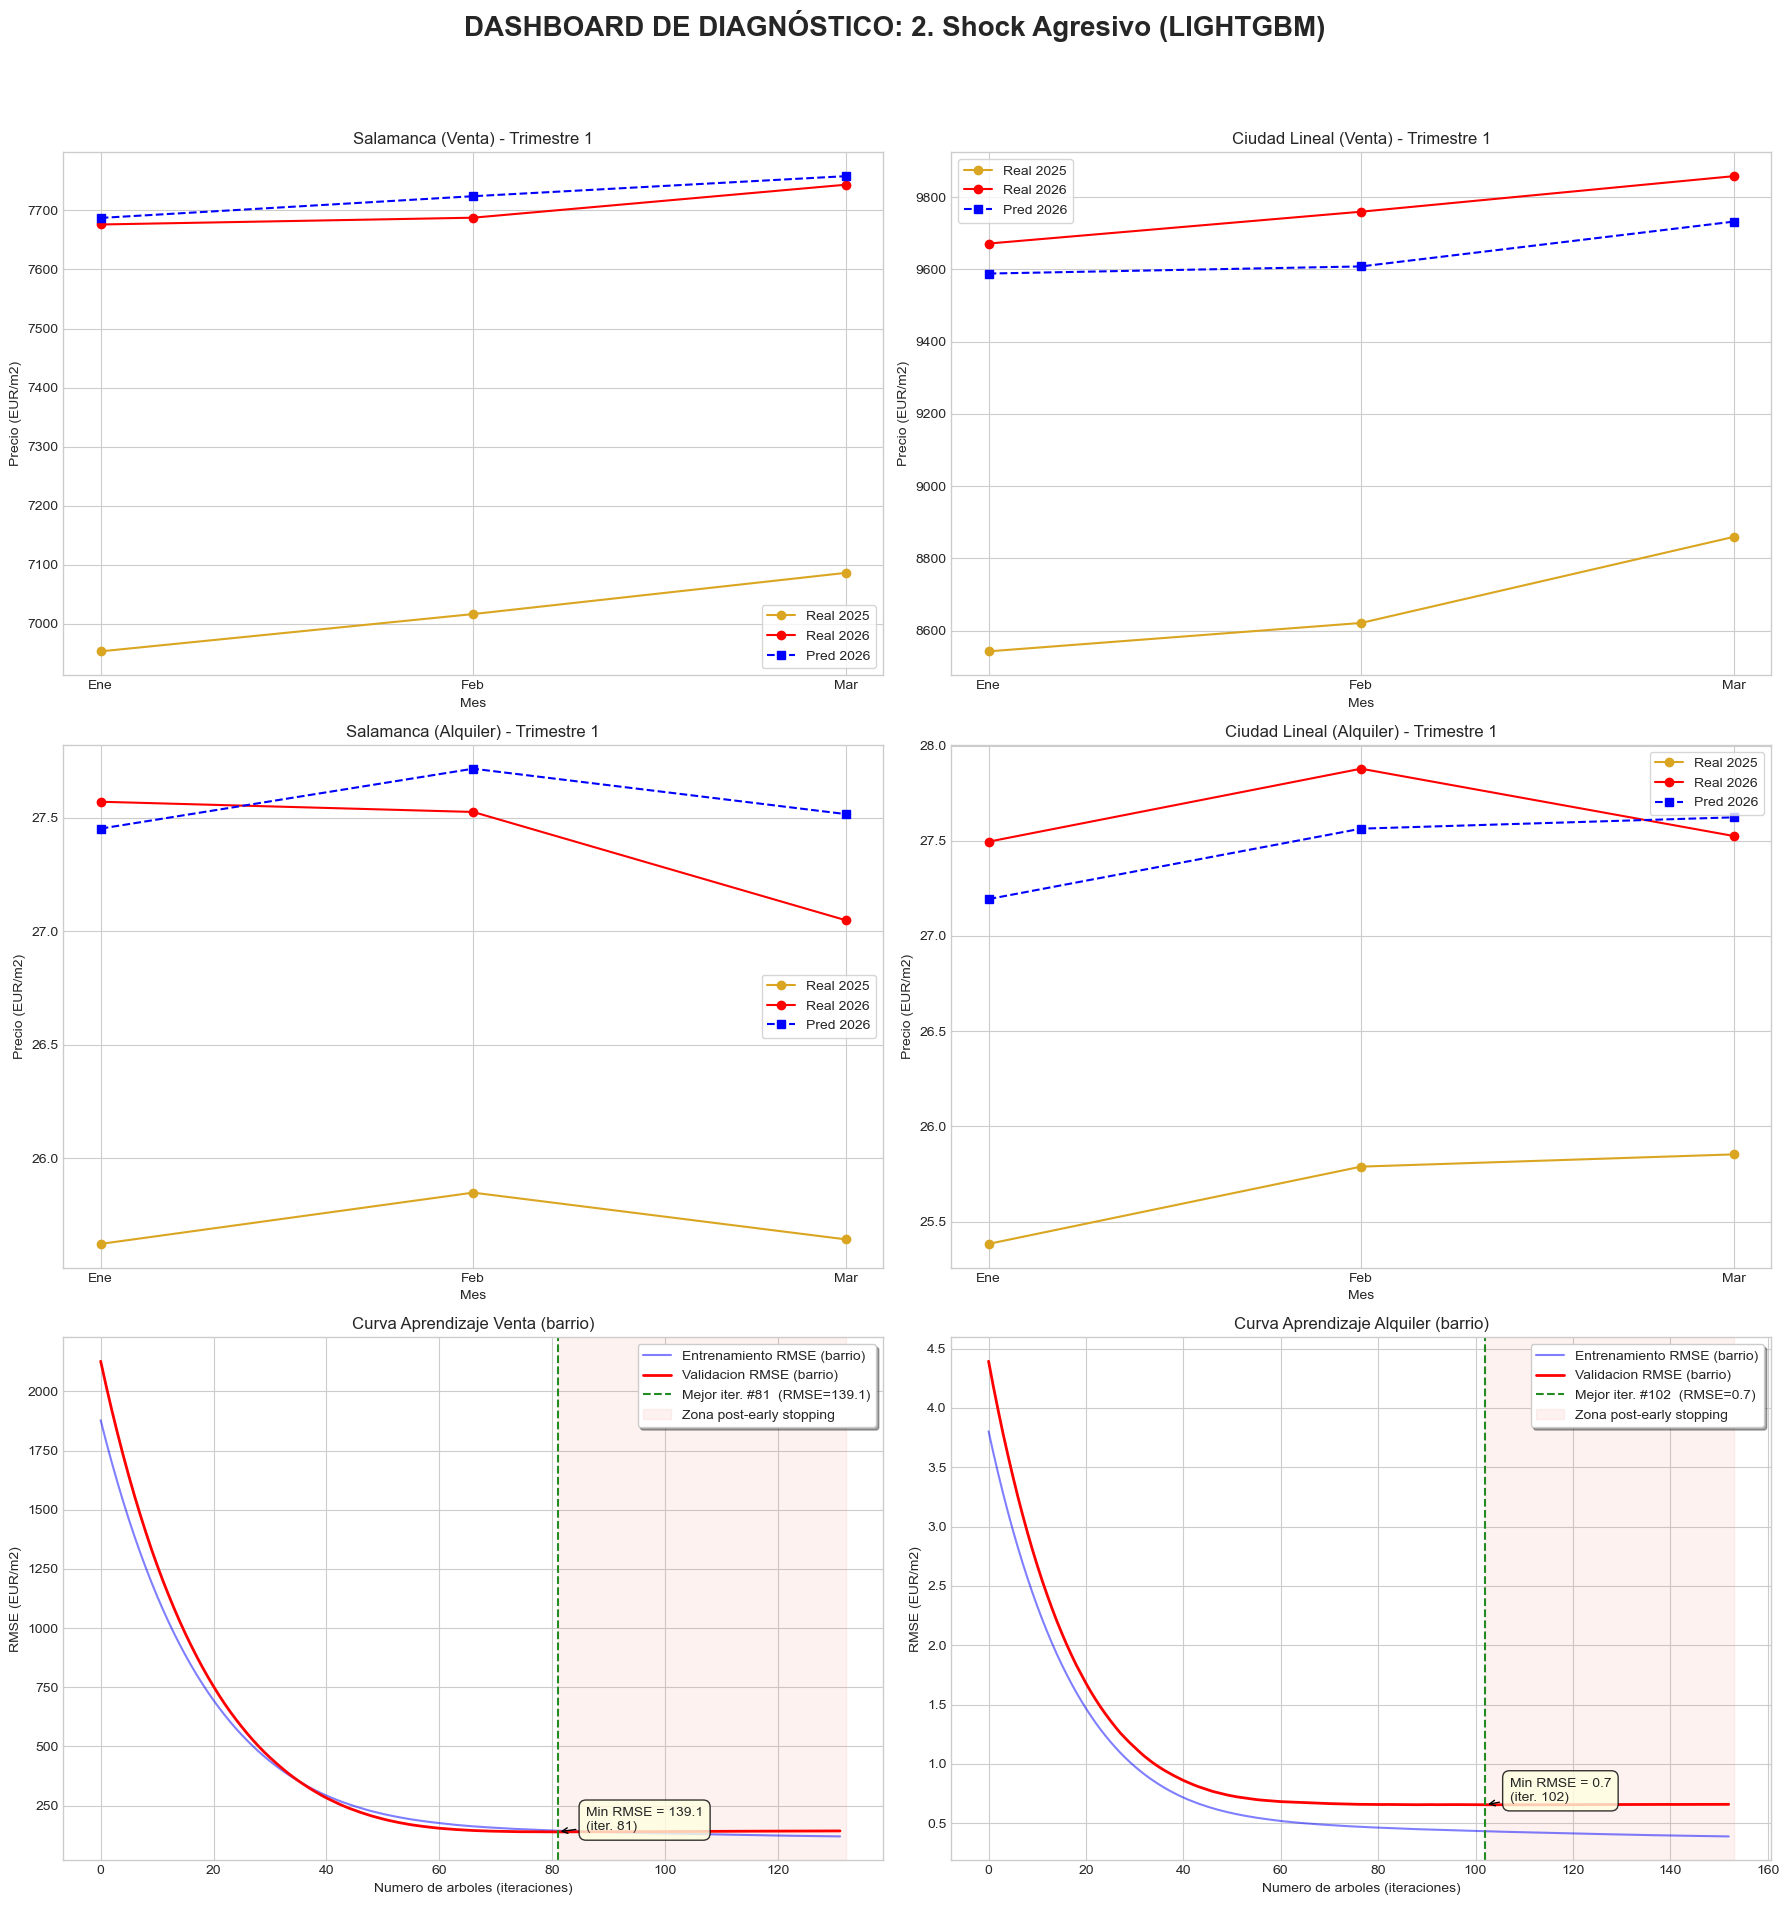
\includegraphics[width=1\linewidth]{img/faseb_agresivo_LightGBM.png}
\caption[Dashboard del Experimento 1 (Shock Agresivo) - LightGBM]{Dashboard comparativo del Experimento 1 (Shock Agresivo): Ajuste real vs. predicho y curva de aprendizaje para LightGBM.}
\label{fig:db_faseb_agresivo_lgb}
\end{figure}

\begin{figure}[H]
\centering
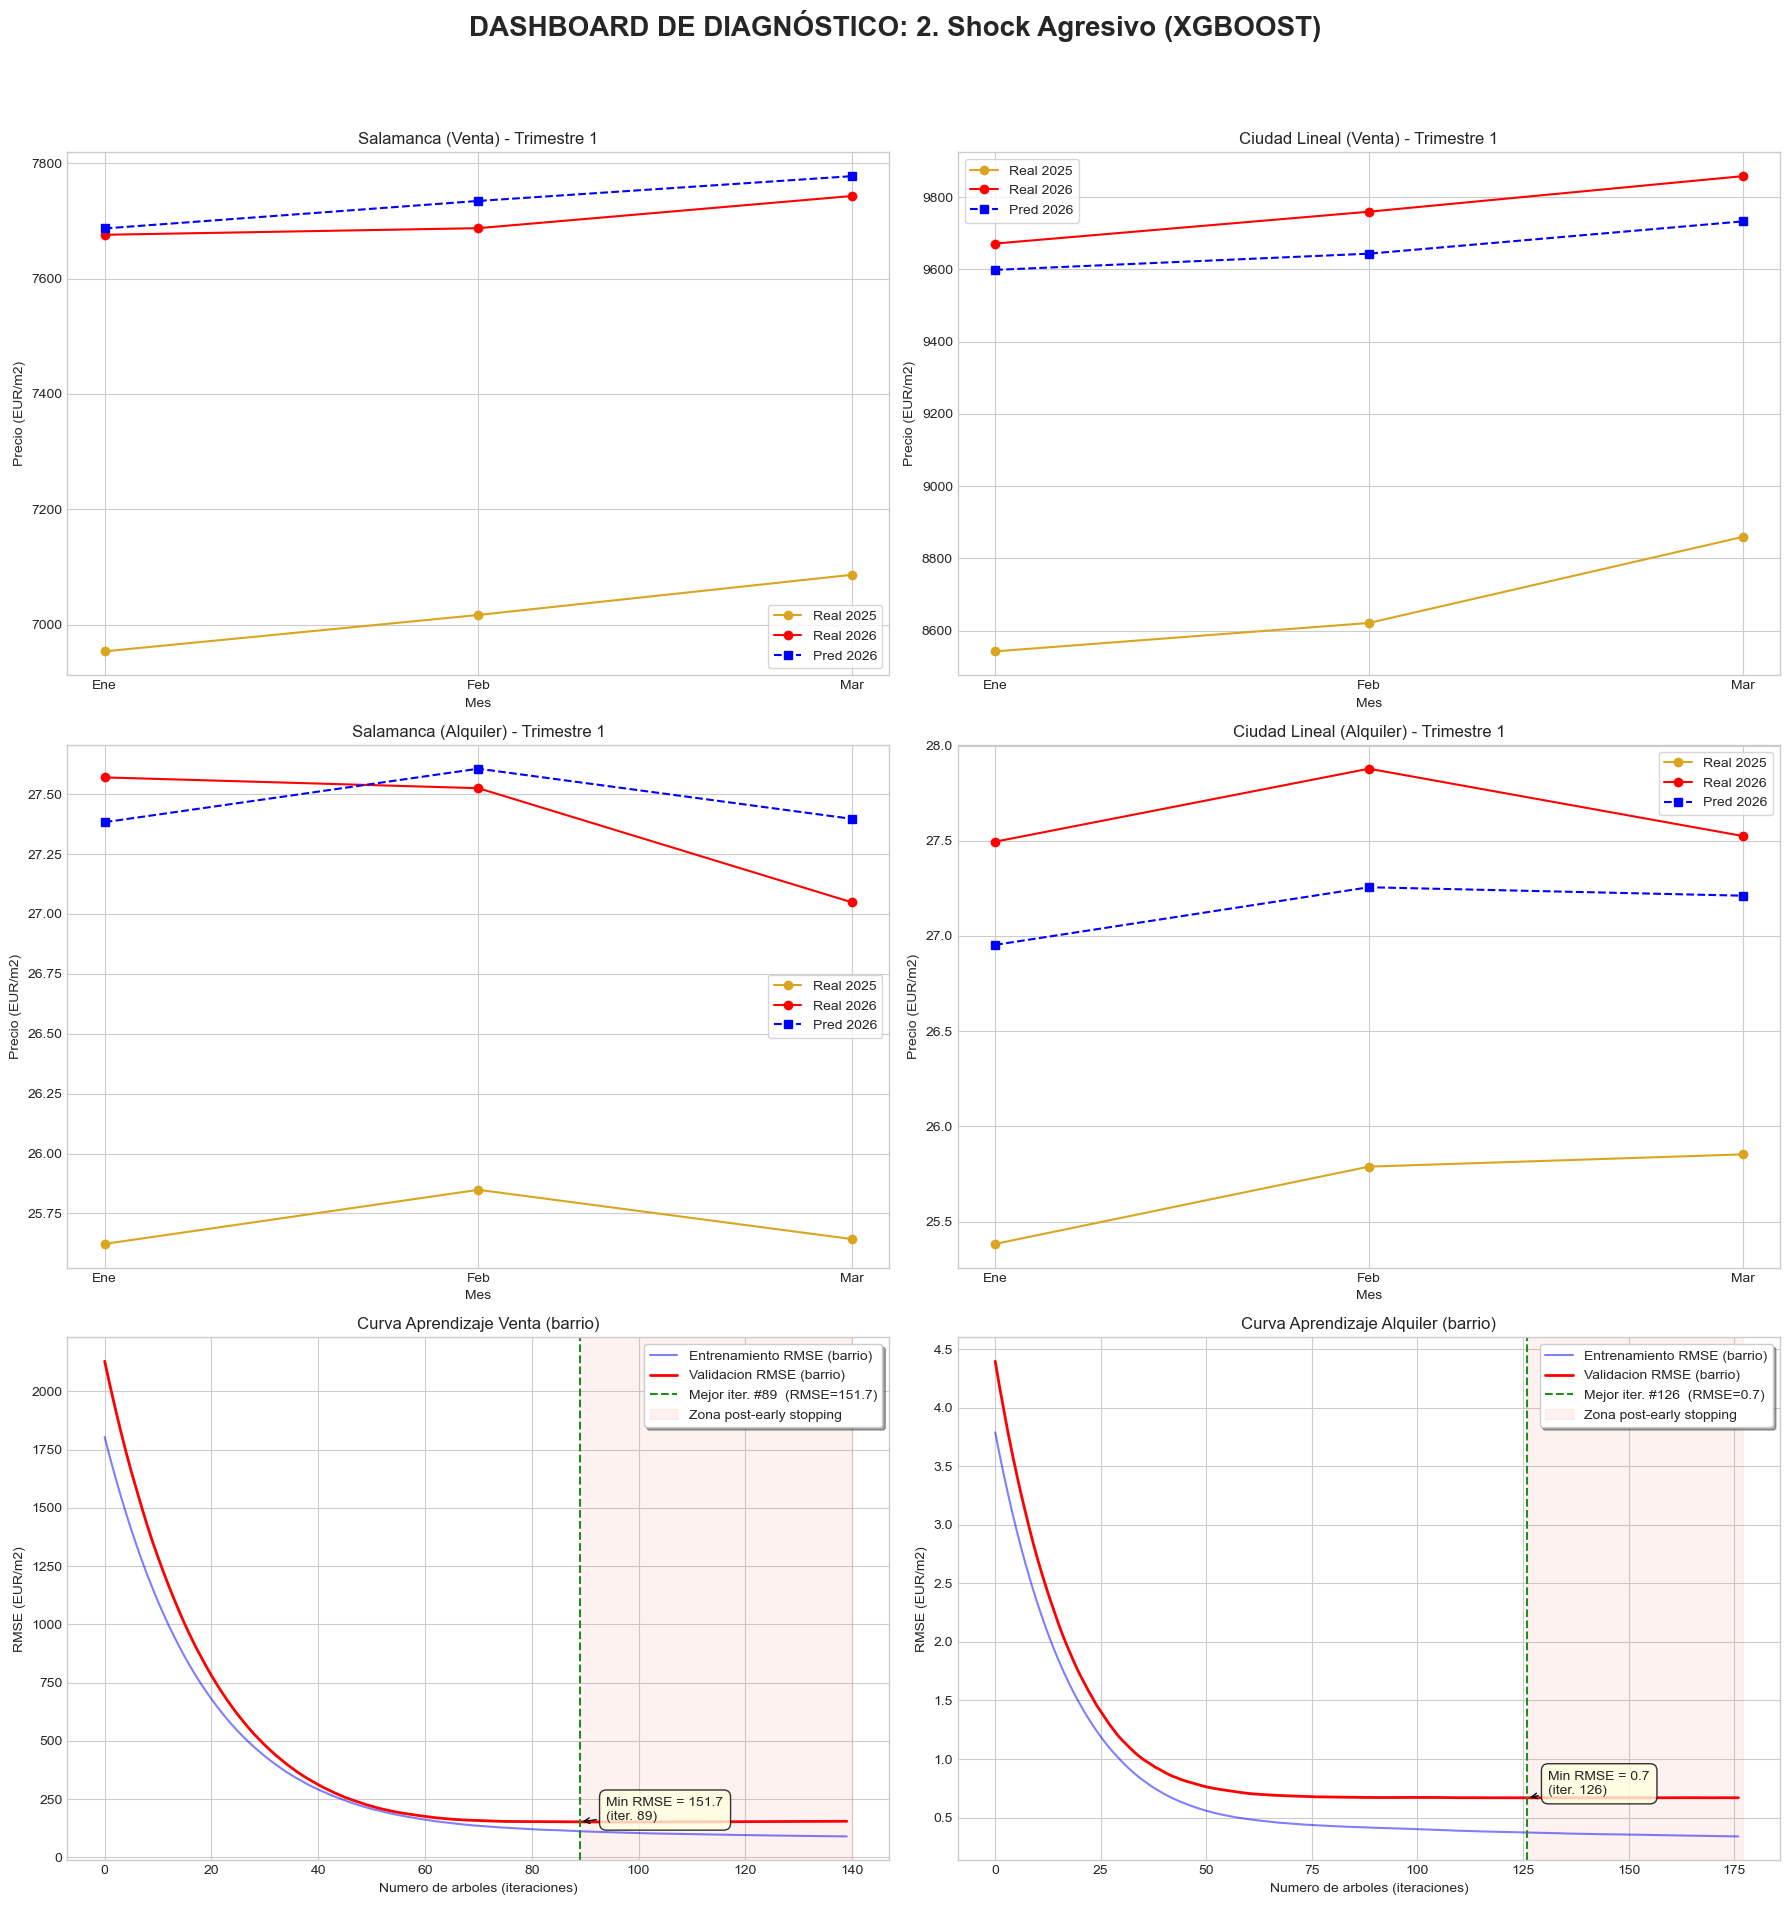
\includegraphics[width=1\linewidth]{img/faseb_agresivo_XGBoost.png}
\caption[Dashboard del Experimento 1 (Shock Agresivo) - XGBoost]{Dashboard comparativo del Experimento 1 (Shock Agresivo): Ajuste real vs. predicho y curva de aprendizaje para XGBoost.}
\label{fig:db_faseb_agresivo_xgb}
\end{figure}

\begin{figure}[H]
\centering
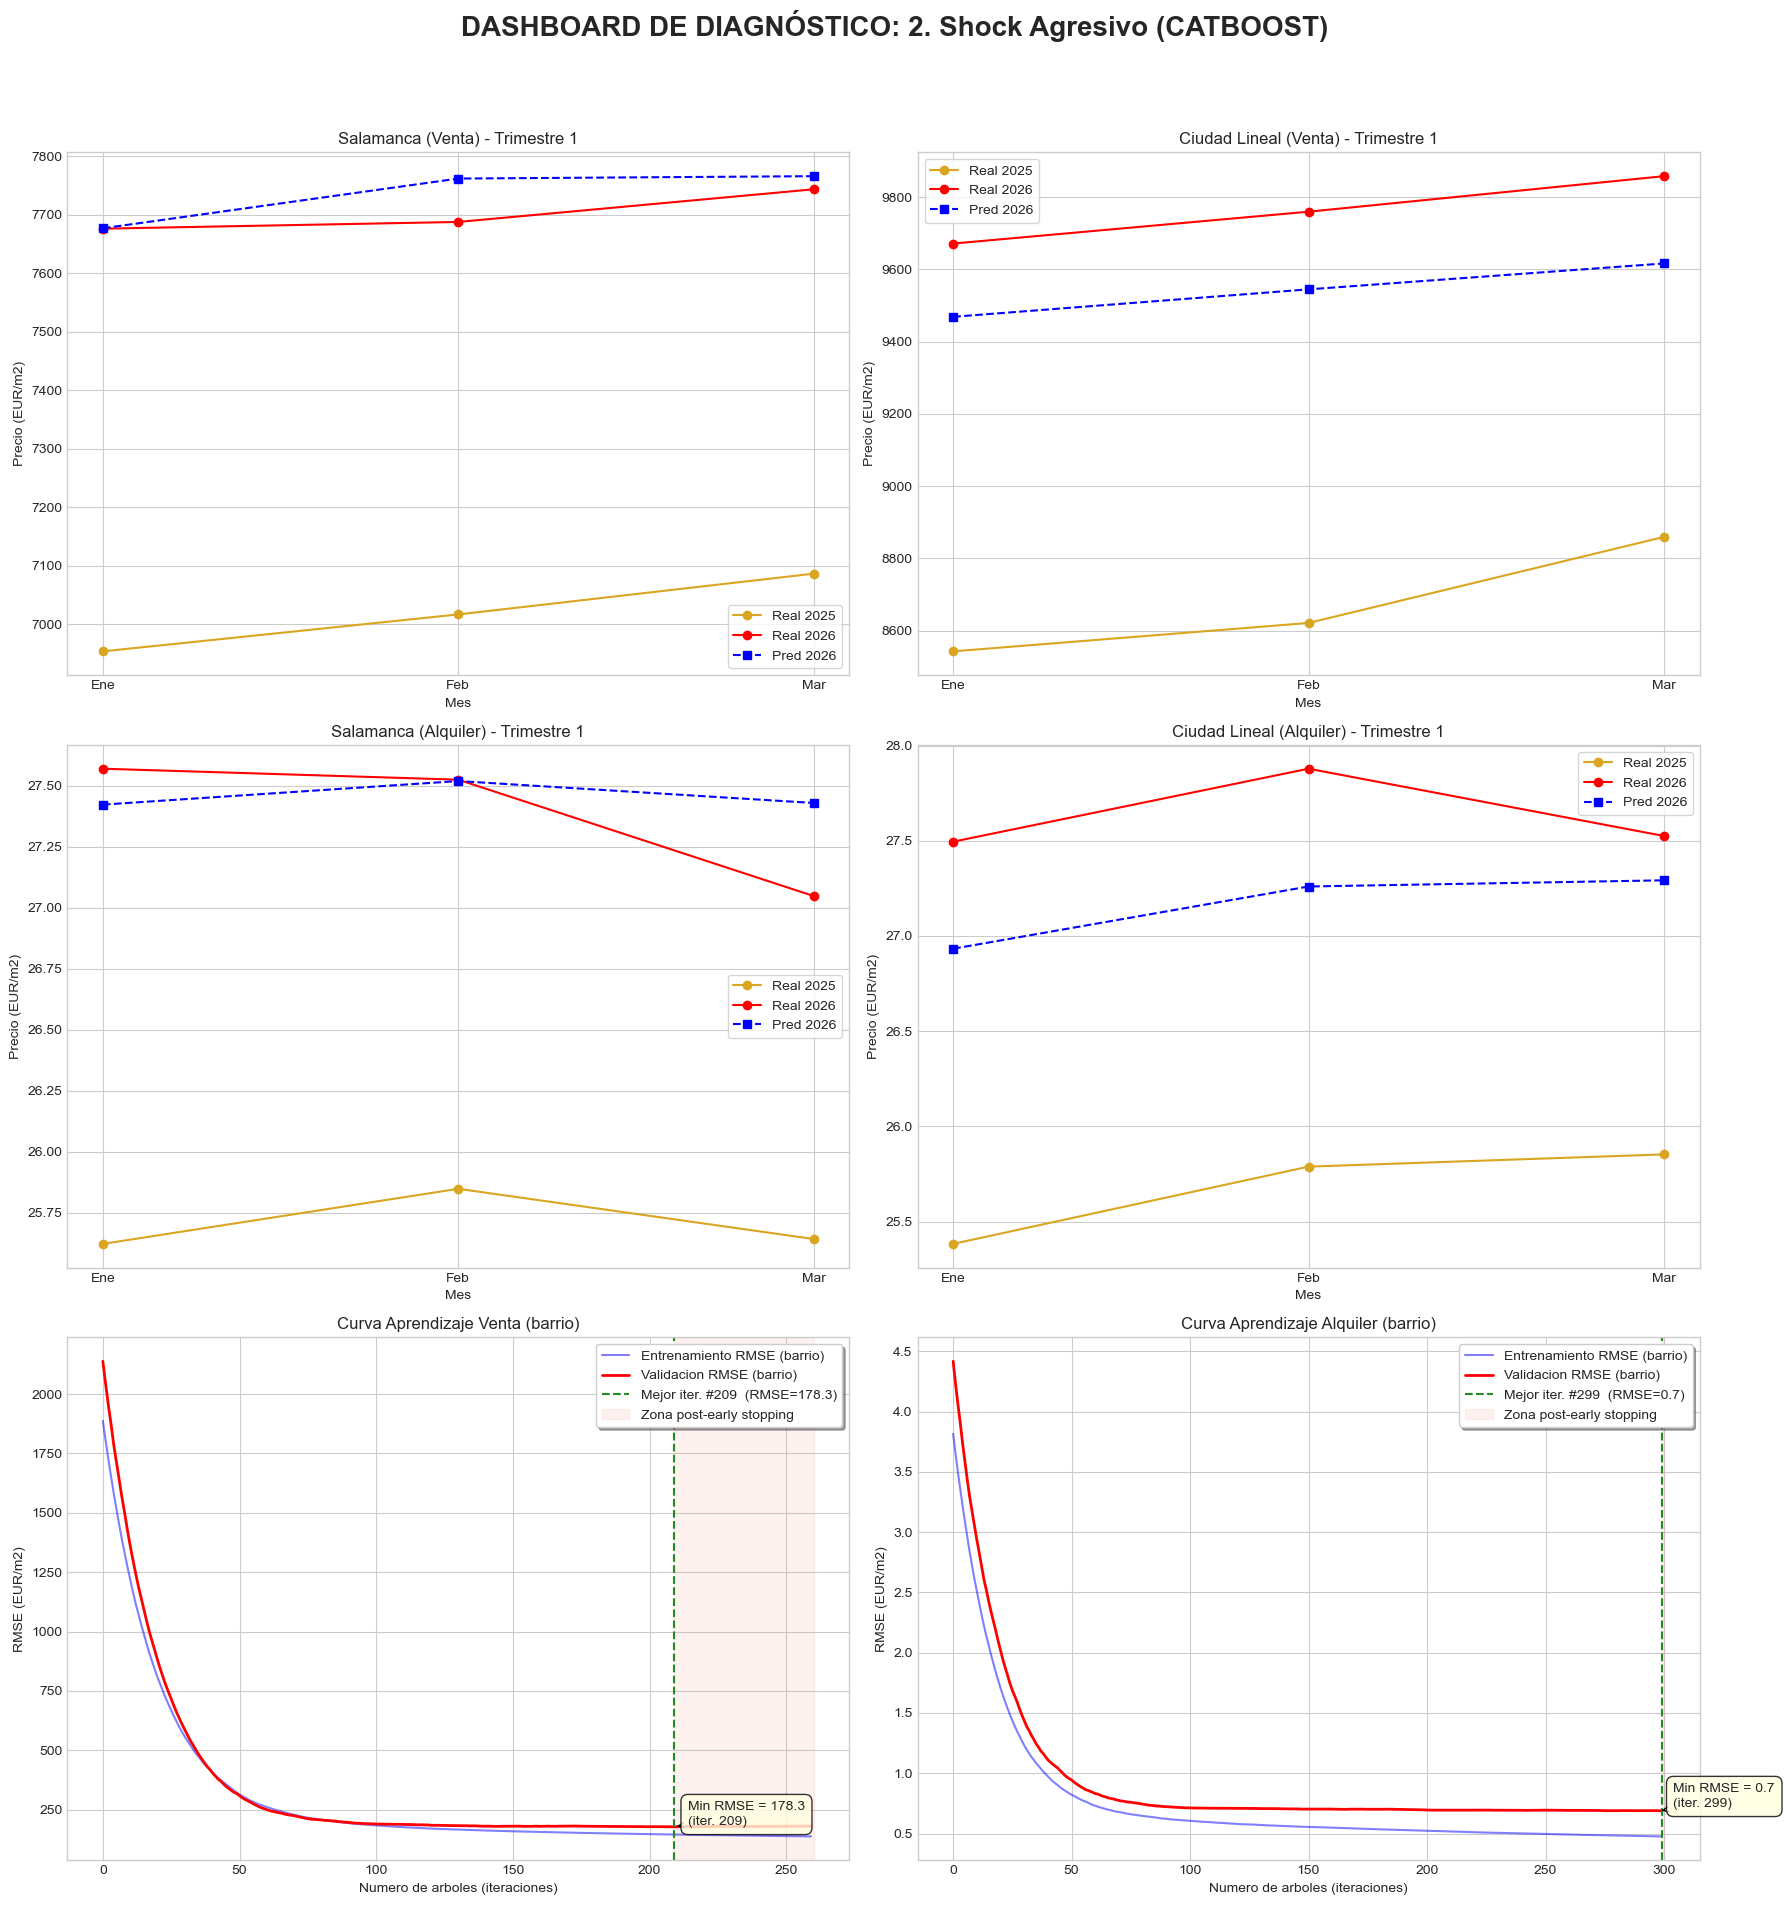
\includegraphics[width=1\linewidth]{img/faseb_agresivo_CatBoost.png}
\caption[Dashboard del Experimento 1 (Shock Agresivo) - CatBoost]{Dashboard comparativo del Experimento 1 (Shock Agresivo): Ajuste real vs. predicho y curva de aprendizaje para CatBoost.}
\label{fig:db_faseb_agresivo_cat}
\end{figure}

El análisis de los dashboards de diagnóstico para el Experimento 1 (Shock Agresivo) revela las siguientes características en el aprendizaje y la inferencia temporal de los modelos:
\begin{itemize}
    \item \textbf{Random Forest (Figura~\ref{fig:db_faseb_agresivo_rf}):} En el mercado de venta, el algoritmo continúa exhibiendo un patrón ruidoso de curvas de aprendizaje con signos de subajuste (\textit{underfitting}), donde la línea de validación se sitúa por debajo de la de entrenamiento. A nivel de venta micro-local (Salamanca y Ciudad Lineal) las estimaciones siguen perdiendo resolución analítica al no poder corregir adecuadamente la varianza temporal. Por su parte, en alquiler la validación se mantiene por encima del entrenamiento de forma estable, confirmando que tiende a generalizar un poco mejor bajo este peso, aunque su RMSE mínimo de 0,62 €/m\textsuperscript{2} (árbol 79) es similar al de las fases previas.
    \item \textbf{LightGBM (Figura~\ref{fig:db_faseb_agresivo_lgb}):} Exhibe una capacidad de generalización moderada en el rango de iteraciones 40 a 50. Sin embargo, a partir de la iteración 80 la curva de validación inicia un ascenso gradual de error. En venta, su óptimo se fija en el árbol 81 (RMSE de 139,11 €/m\textsuperscript{2}). En alquiler, la validación se mantiene por encima del entrenamiento de forma estable, localizando la mejor iteración en la 102 (RMSE mínimo de 0,65 €/m\textsuperscript{2}). En términos de ajuste real vs. predicho, Salamanca y Ciudad Lineal muestran predicciones muy bien acopladas con curvas muy cercanas que respetan las tendencias del mercado.
    \item \textbf{XGBoost (Figura~\ref{fig:db_faseb_agresivo_xgb}):} Reporta una curva de aprendizaje de alta calidad, manteniéndose muy cerca del entrenamiento en la ventana de iteraciones 40 a 80. En venta, su early stopping se sitúa en la iteración 89 con un RMSE de 151,68 €/m\textsuperscript{2}, requiriendo más árboles y un entrenamiento más prolongado que LightGBM. En alquiler, el comportamiento se estabiliza con una mejor iteración similar, aunque con un RMSE promedio comparable. Las proyecciones muestran una ligera sobreestimación en Salamanca venta y estimaciones conservadoras en alquiler, respetando adecuadamente los giros estacionales de la serie.
    \item \textbf{CatBoost (Figura~\ref{fig:db_faseb_agresivo_cat}):} Muestra curvas de aprendizaje sumamente estables donde la validación solapa de manera limpia al entrenamiento, descartando cualquier indicio de subajuste y confirmando una óptima capacidad de generalización. La curva de validación inicia una leve deriva alcista a partir del árbol 100. En venta, CatBoost dilata significativamente su aprendizaje, requiriendo un mayor número de estimadores pero reportando un RMSE final superior (178,30 €/m\textsuperscript{2}). En alquiler, la iteración óptima se desplaza hasta el final de la ventana de early stopping, reportando un RMSE de 0,69 €/m\textsuperscript{2}.
\end{itemize}

\subsubsection{Experimento 2: Shock Progresivo (Rampa Lineal)}
En este experimento se diseña e implementa una estrategia híbrida bidimensional para guiar el aprendizaje de los modelos en presencia del cambio estructural observado. Esta estrategia combina dos mecanismos complementarios:

\begin{enumerate}
    \item \textbf{Inyección de Variable Predictora (Feature Engineering):} Se inyecta una variable de ingeniería temporal denominada \textbf{Shock Weight} ($SW_t$), la cual actúa como una rampa lineal progresiva que indica al modelo el grado de maduración o penetración del shock a lo largo del tiempo. Esta variable se define matemáticamente mediante la siguiente función por tramos:
    \begin{equation}
    SW_t = \begin{cases} 
    0.0 & \text{para los años 2023 y 2024 (periodo pre-shock)} \\
    \frac{\text{mes}}{12} & \text{para los meses del año 2025 (rampa lineal de shock)} \\
    1.0 & \text{constante a partir de enero de 2026 (régimen post-shock)}
    \end{cases}
    \end{equation}
    Donde $\text{mes} \in [1, 12]$ representa el mes de ejecución del año 2025. Al entrenar con esta columna, el modelo aprende la pendiente del shock y puede extrapolar con un valor estable de $1.0$ durante las predicciones del horizonte de test de 2026.
    
    \item \textbf{Ponderación Temporal de Muestras (Sample Weighting):} Simultáneamente, para favorecer la adaptación al \textit{Concept Drift} sin perder el histórico completo de los años anteriores, se aplica un esquema de pesos de entrenamiento progresivo en la función de pérdida de los algoritmos. En comparación con el peso estático del Experimento 1, se asigna una ponderación creciente a las observaciones conforme se aproximan al periodo de shock y post-shock:
    \begin{equation}
    w_t = \begin{cases} 
    1.0 & \text{para las observaciones del año 2023} \\
    1.2 & \text{para las observaciones del año 2024} \\
    1.8 & \text{para las observaciones del año 2025} \\
    2.5 & \text{para las observaciones del año 2026}
    \end{cases}
    \end{equation}
\end{enumerate}

Esta formulación matemática actúa como un potenciómetro que guía el aprendizaje del modelo out-of-sample en el régimen de 2026, lo que evita la subestimación sistemática provocada por la inercia del pasado. Las métricas resultantes se detallan en la Tabla~\ref{tab:fase_b_exp2_venta} para el mercado de venta y en la Tabla~\ref{tab:fase_b_exp2_alquiler} para el mercado de alquiler.

\begin{table}[H]
\centering
\resizebox{\textwidth}{!}{%
\begin{tabular}{|l|c|c|c|c|c|c|c|c|c|}
\hline
\textbf{Algoritmo} & \textbf{MAE Global} & \textbf{RMSE Global} & \textbf{R\textsuperscript{2} Global} & \textbf{MAE Salam.} & \textbf{R\textsuperscript{2} Salam.} & \textbf{MAE C. Lineal} & \textbf{R\textsuperscript{2} C. Lineal} & \textbf{T. Train (s)} & \textbf{T. Pred (s)} \\
 & \textbf{(€/m\textsuperscript{2})} & \textbf{(€/m\textsuperscript{2})} & & \textbf{(€/m\textsuperscript{2})} & & \textbf{(€/m\textsuperscript{2})} & & & \\
\hline
\textbf{Random Forest} & 98,99 & 136,75 & 0,9956 & 109,18 & 0,9717 & 132,83 & 0,9876 & 1,2045 & 0,0402 \\
\textbf{LightGBM} & 103,44 & 139,15 & 0,9955 & 70,80 & 0,9859 & 209,50 & 0,9711 & 0,1989 & 0,0020 \\
\textbf{XGBoost} & 103,92 & 145,35 & 0,9951 & 102,68 & 0,9627 & 147,88 & 0,9852 & 1,4708 & 0,0164 \\
\textbf{CatBoost} & 125,61 & 175,78 & 0,9928 & 108,52 & 0,9755 & 324,52 & 0,9404 & 1,2730 & 0,0023 \\
\hline
\end{tabular}%
}
\caption{Métricas obtenidas en el Mercado de Venta para el Experimento 2 (Shock Progresivo con Rampa Lineal $1/12$ en 2025 y $1.0$ en 2026).}
\label{tab:fase_b_exp2_venta}
\end{table}

\begin{table}[H]
\centering
\resizebox{\textwidth}{!}{%
\begin{tabular}{|l|c|c|c|c|c|c|c|c|c|}
\hline
\textbf{Algoritmo} & \textbf{MAE Global} & \textbf{RMSE Global} & \textbf{R\textsuperscript{2} Global} & \textbf{MAE Salam.} & \textbf{R\textsuperscript{2} Salam.} & \textbf{MAE C. Lineal} & \textbf{R\textsuperscript{2} C. Lineal} & \textbf{T. Train (s)} & \textbf{T. Pred (s)} \\
 & \textbf{(€/m\textsuperscript{2})} & \textbf{(€/m\textsuperscript{2})} & & \textbf{(€/m\textsuperscript{2})} & & \textbf{(€/m\textsuperscript{2})} & & & \\
\hline
\textbf{Random Forest} & 0,4636 & 0,6191 & 0,9744 & 0,4378 & 0,7702 & 0,5047 & 0,9695 & 1,2033 & 0,0451 \\
\textbf{LightGBM} & 0,4832 & 0,6305 & 0,9735 & 0,4469 & 0,7985 & 0,5374 & 0,9572 & 0,1828 & 0,0020 \\
\textbf{XGBoost} & 0,5077 & 0,6698 & 0,9701 & 0,4835 & 0,6842 & 0,7371 & 0,9269 & 0,9971 & 0,0078 \\
\textbf{CatBoost} & 0,5247 & 0,6758 & 0,9695 & 0,4212 & 0,7883 & 0,8416 & 0,9078 & 1,3418 & 0,0025 \\
\hline
\end{tabular}%
}
\caption{Métricas obtenidas en el Mercado de Alquiler para el Experimento 2 (Shock Progresivo con Rampa Lineal $1/12$ en 2025 y $1.0$ en 2026).}
\label{tab:fase_b_exp2_alquiler}
\end{table}

Las figuras~\ref{fig:db_faseb_progresivo_rf}, \ref{fig:db_faseb_progresivo_lgb}, \ref{fig:db_faseb_progresivo_xgb} y \ref{fig:db_faseb_progresivo_cat} ilustran los correspondientes dashboards comparativos en el Experimento 2:

\begin{figure}[H]
\centering
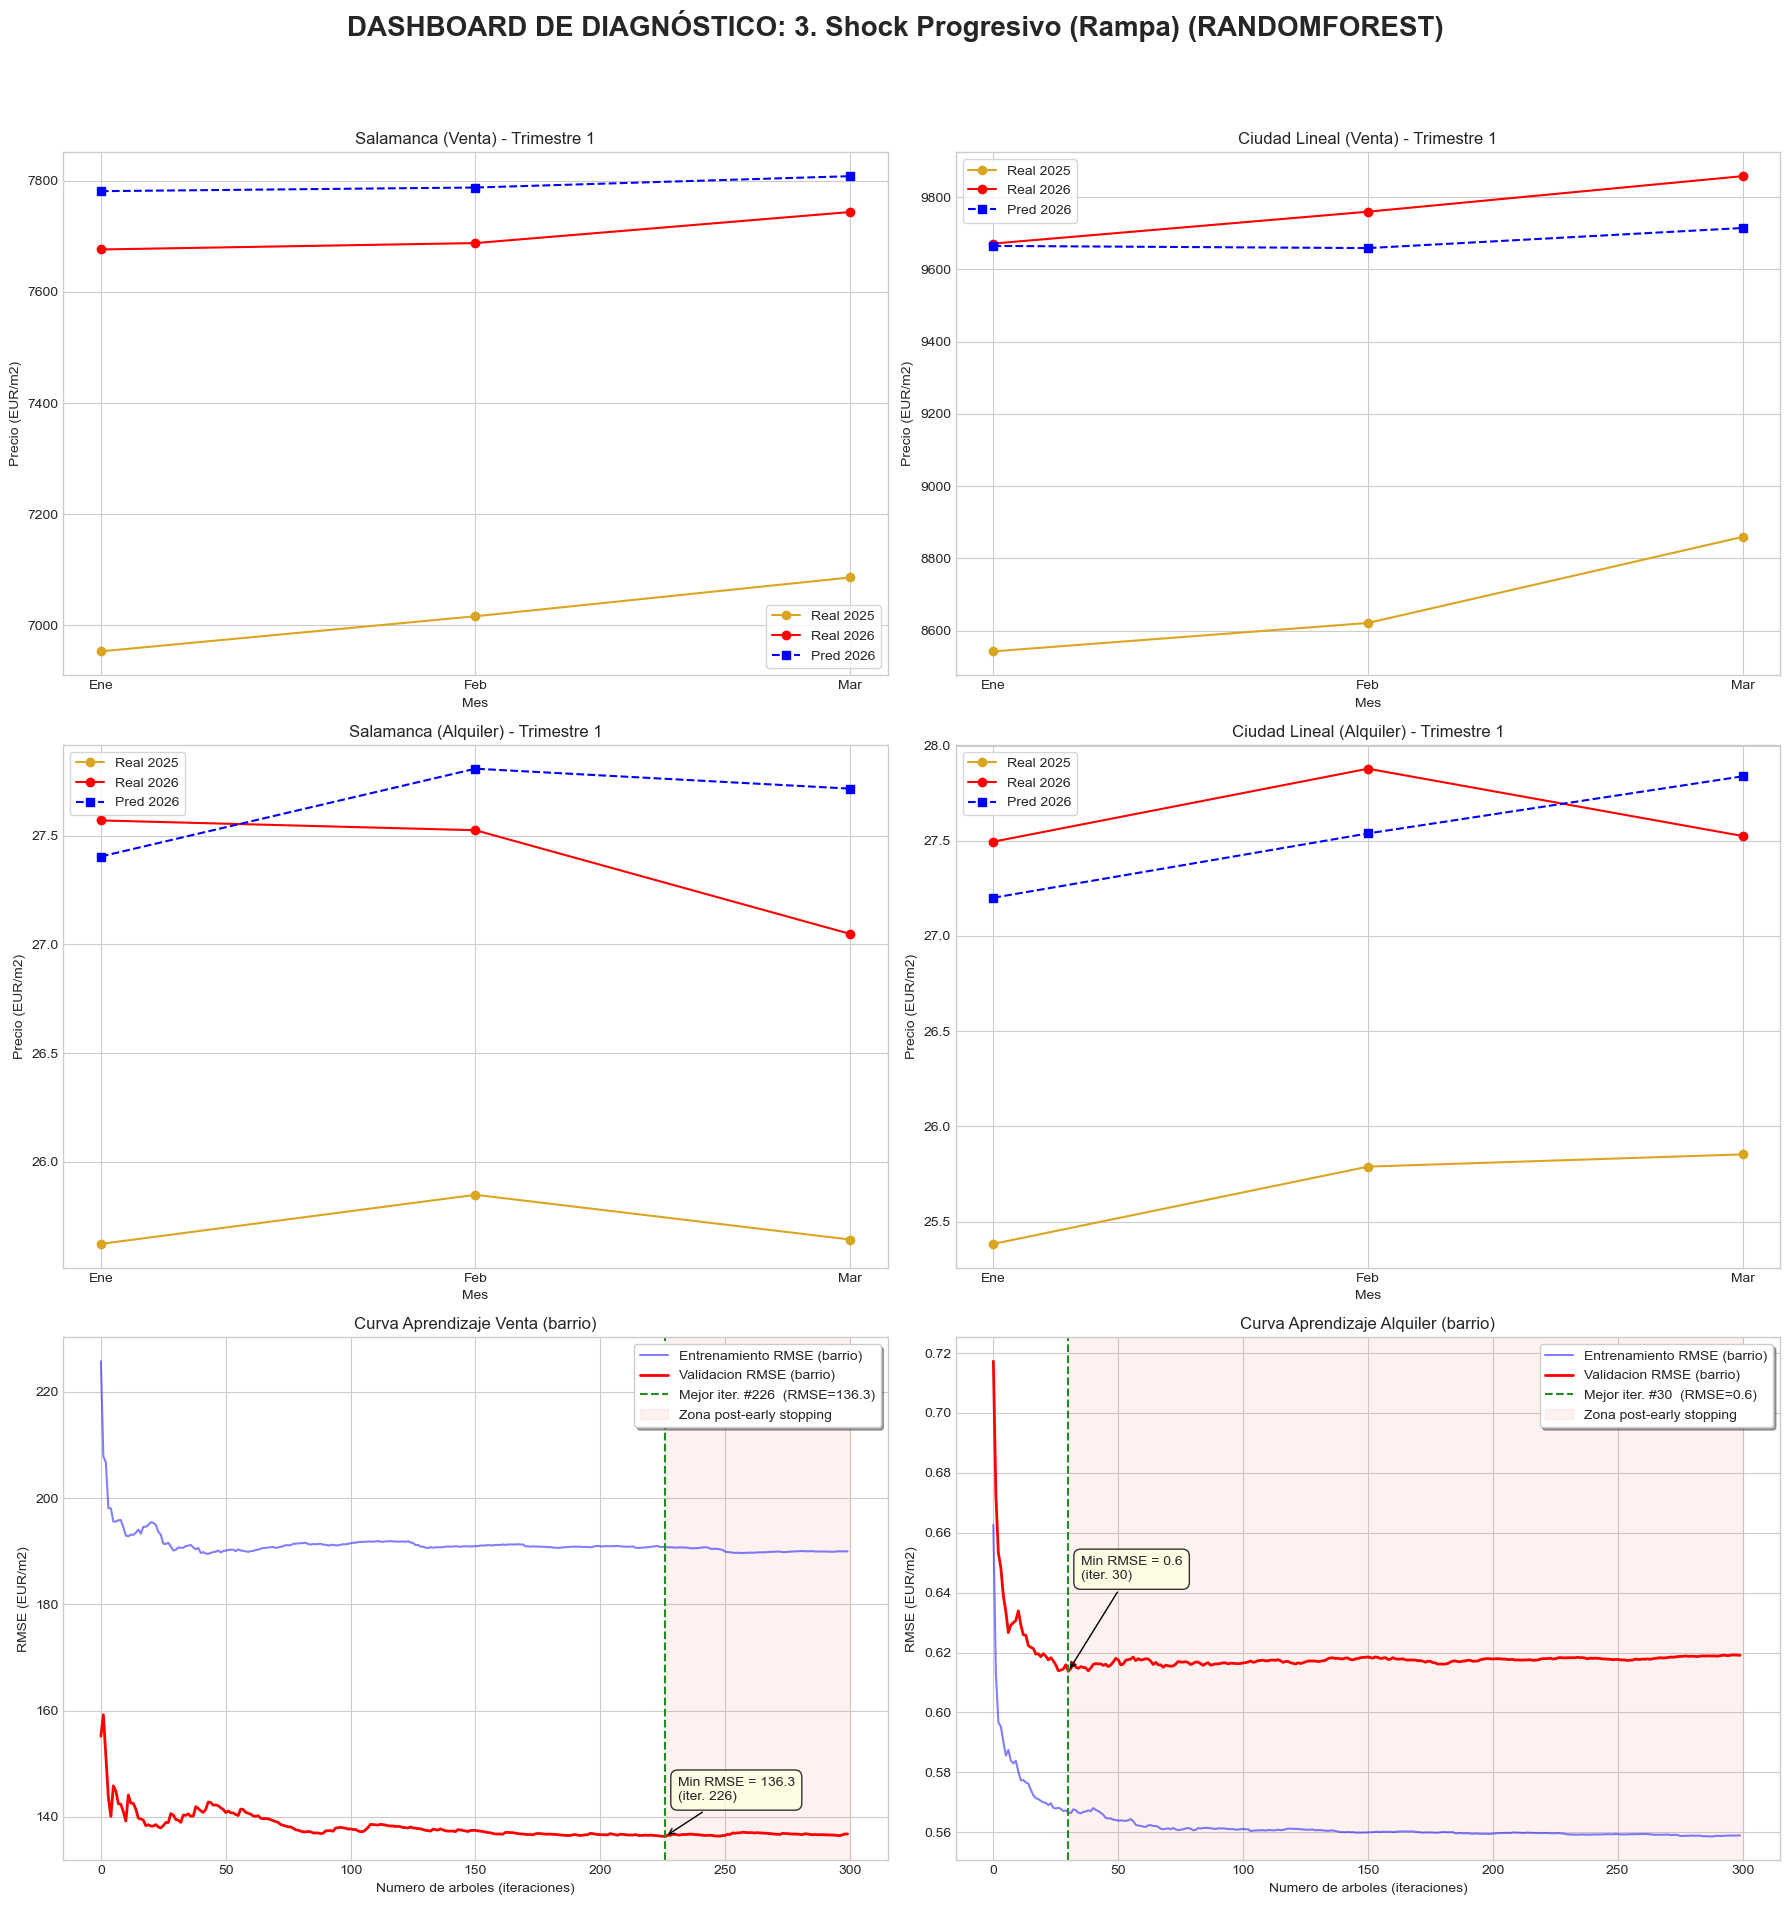
\includegraphics[width=1\linewidth]{img/faseb_progresivo_RandomForest.png}
\caption[Dashboard del Experimento 2 (Shock Progresivo) - Random Forest]{Dashboard comparativo del Experimento 2 (Shock Progresivo): Ajuste real vs. predicho y curva de aprendizaje para Random Forest.}
\label{fig:db_faseb_progresivo_rf}
\end{figure}

\begin{figure}[H]
\centering
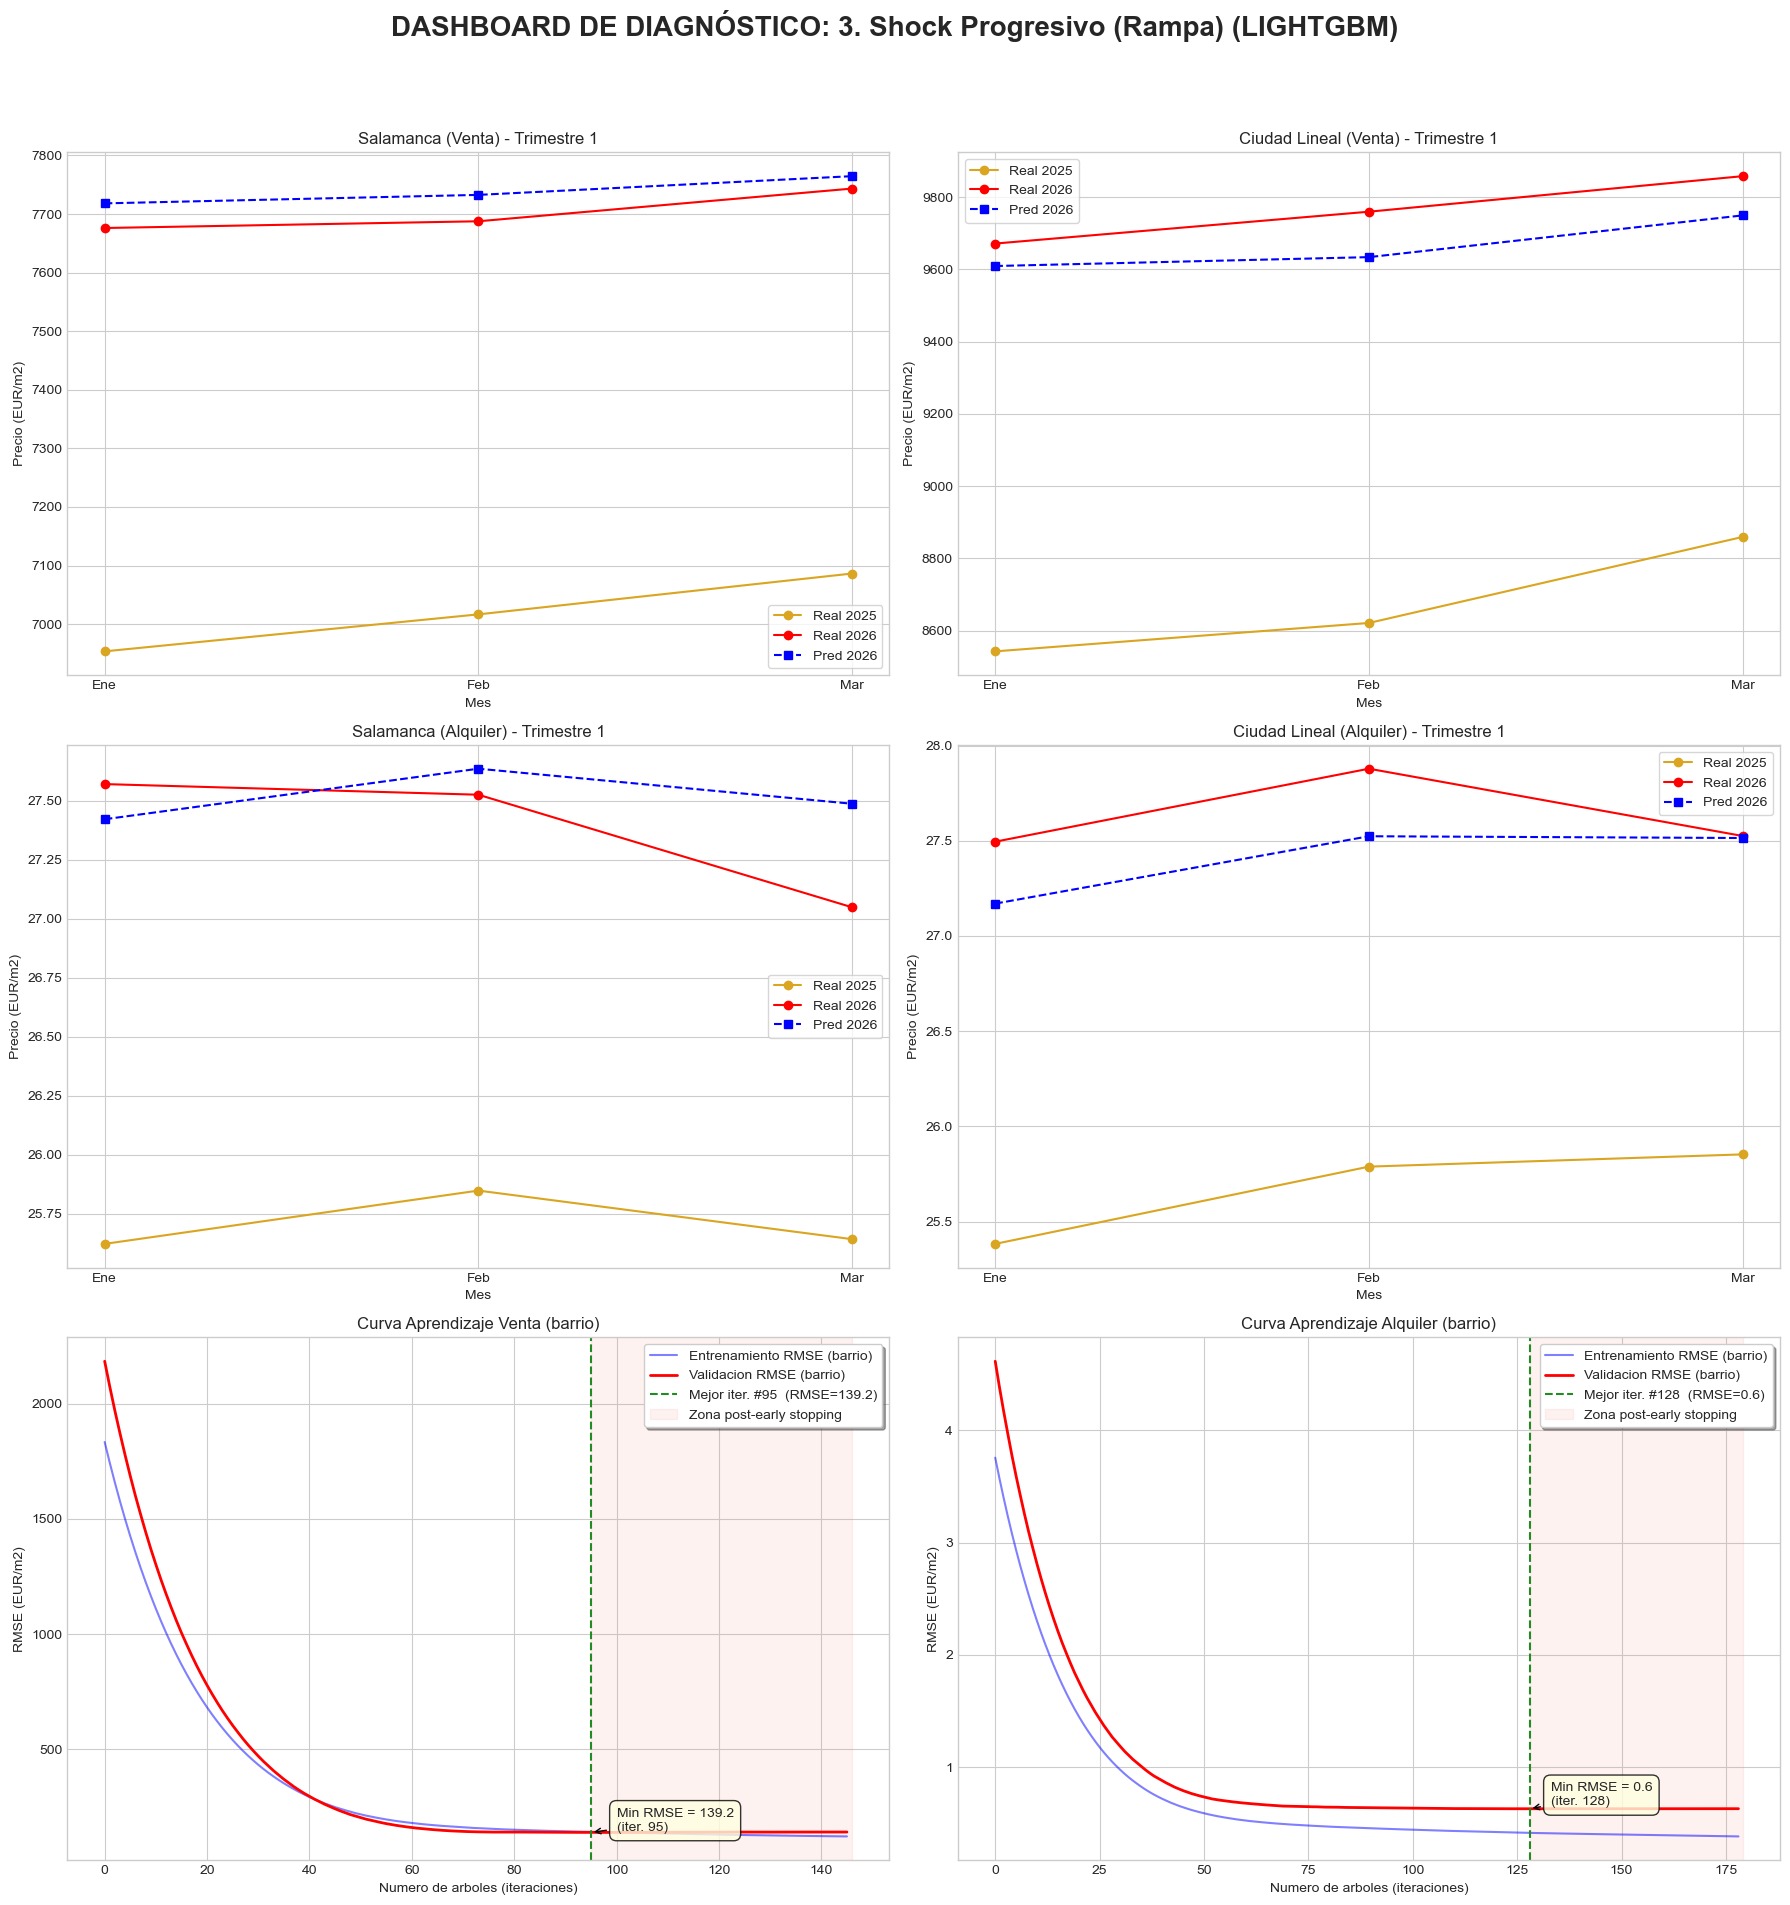
\includegraphics[width=1\linewidth]{img/faseb_progresivo_LightGBM.png}
\caption[Dashboard del Experimento 2 (Shock Progresivo) - LightGBM]{Dashboard comparativo del Experimento 2 (Shock Progresivo): Ajuste real vs. predicho y curva de aprendizaje para LightGBM.}
\label{fig:db_faseb_progresivo_lgb}
\end{figure}

\begin{figure}[H]
\centering
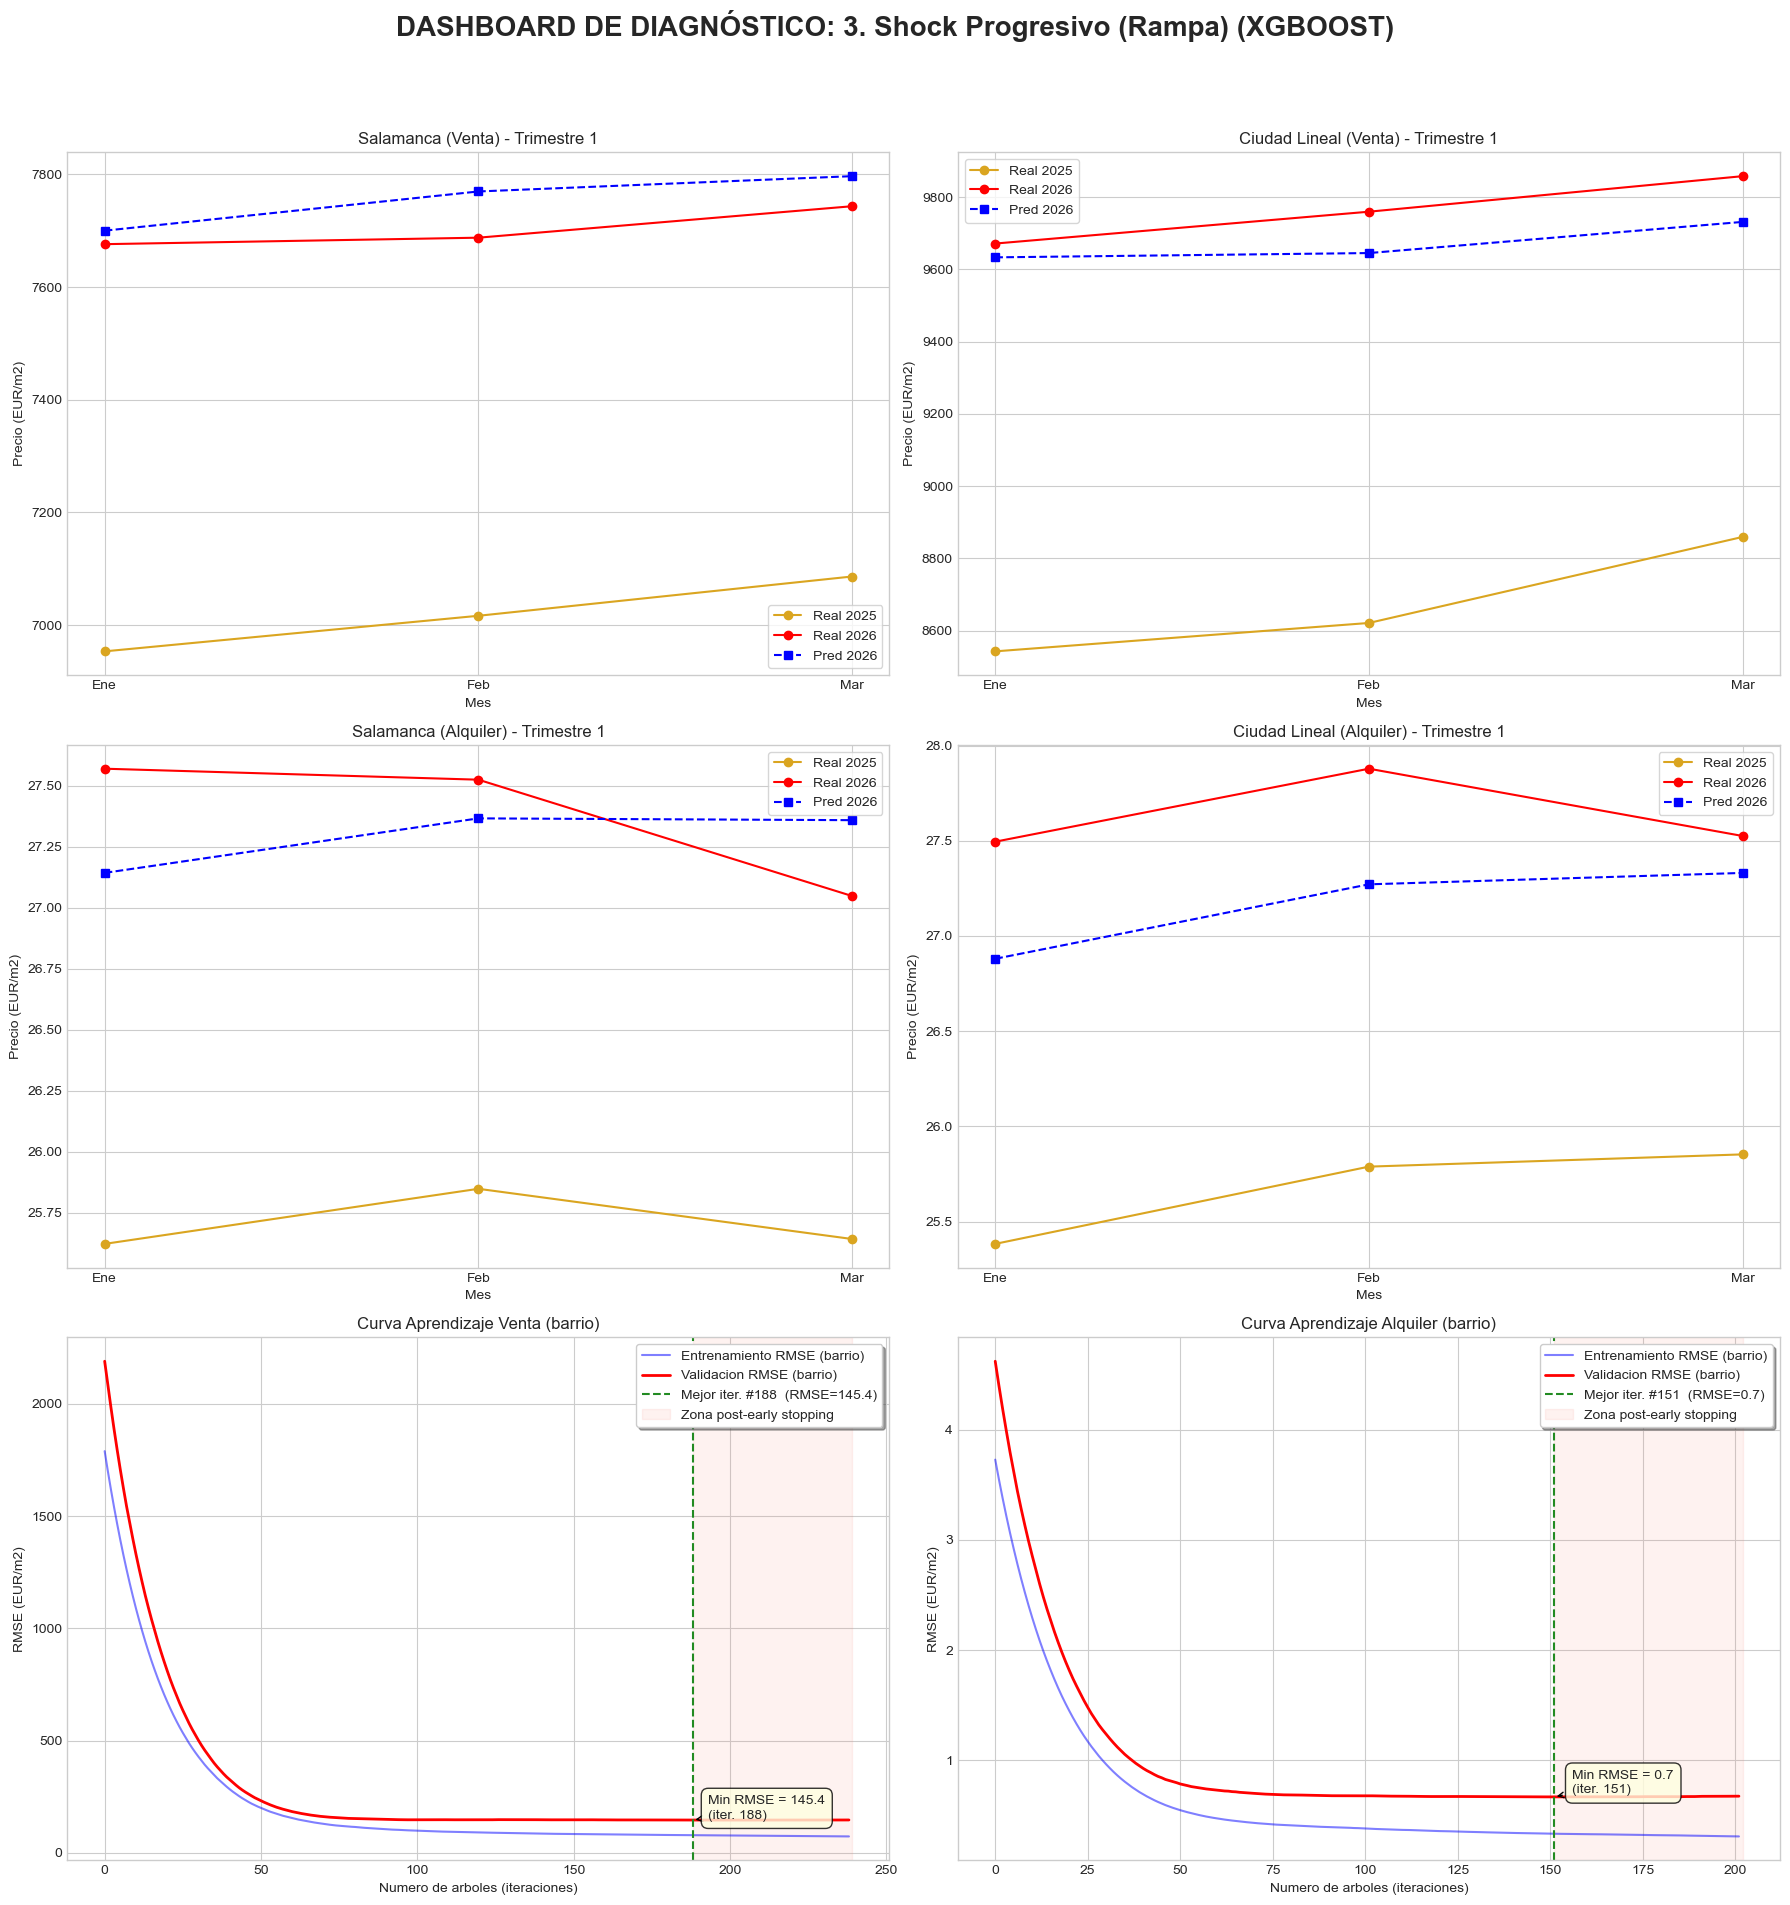
\includegraphics[width=1\linewidth]{img/faseb_progresivo_XGBoost.png}
\caption[Dashboard del Experimento 2 (Shock Progresivo) - XGBoost]{Dashboard comparativo del Experimento 2 (Shock Progresivo): Ajuste real vs. predicho y curva de aprendizaje para XGBoost.}
\label{fig:db_faseb_progresivo_xgb}
\end{figure}

\begin{figure}[H]
\centering
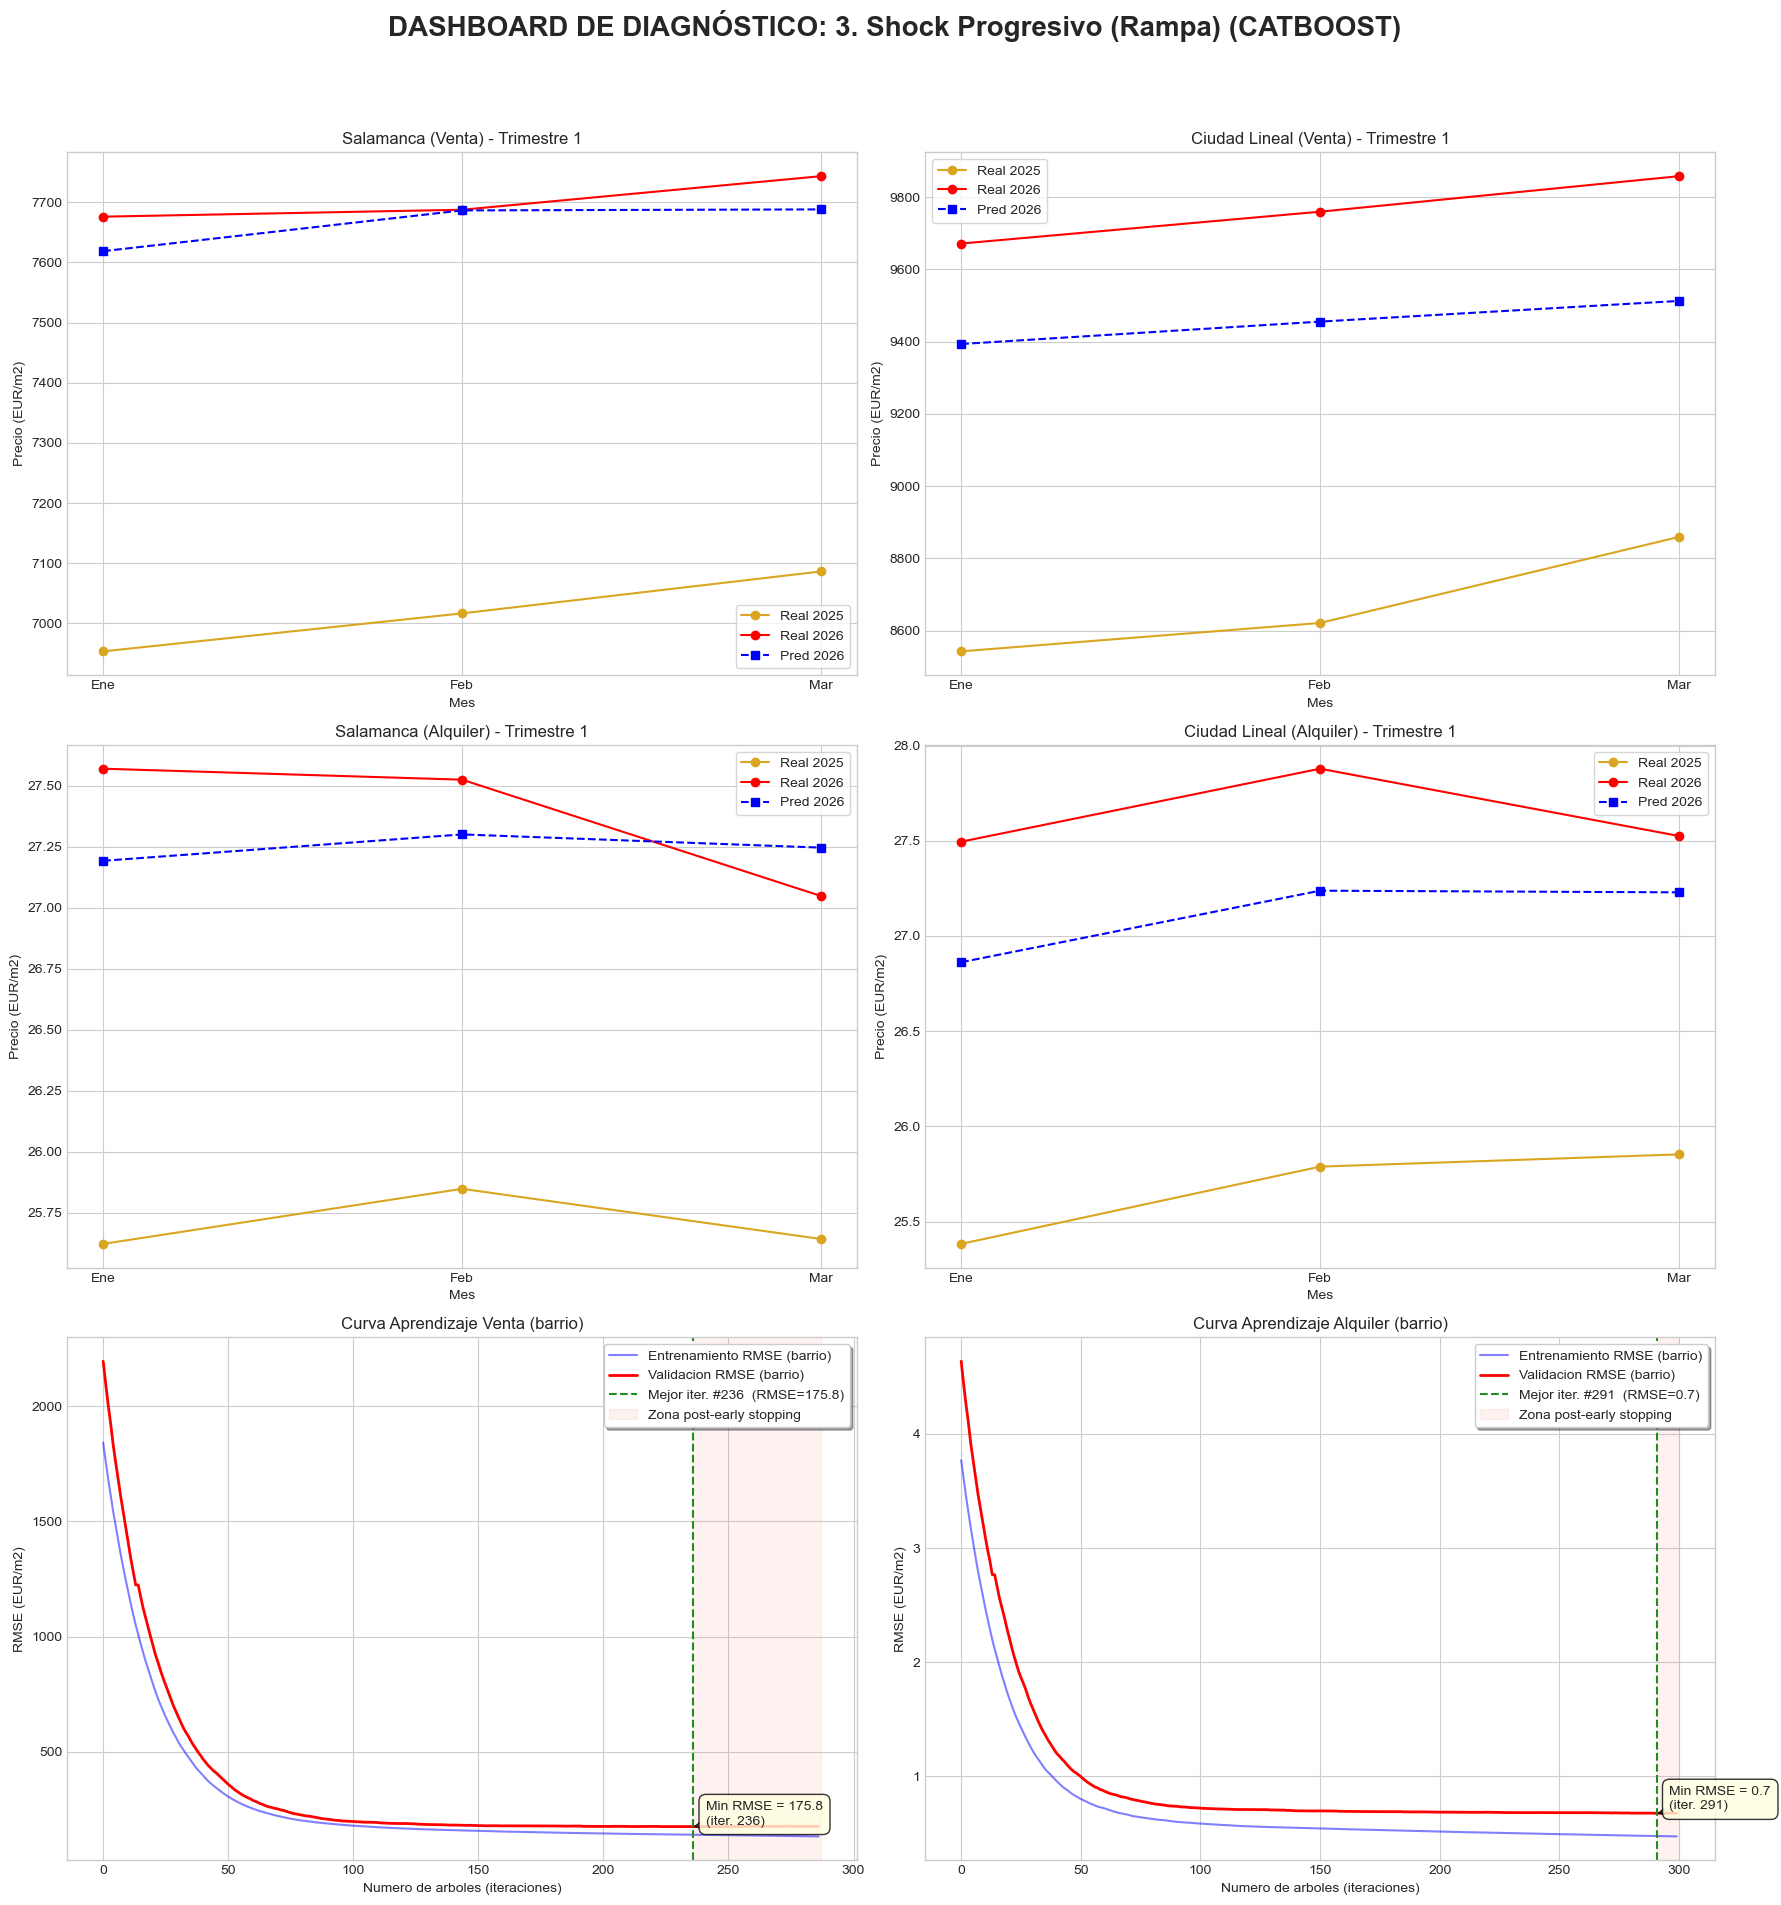
\includegraphics[width=1\linewidth]{img/faseb_progresivo_CatBoost.png}
\caption[Dashboard del Experimento 2 (Shock Progresivo) - CatBoost]{Dashboard comparativo del Experimento 2 (Shock Progresivo): Ajuste real vs. predicho y curva de aprendizaje para CatBoost.}
\label{fig:db_faseb_progresivo_cat}
\end{figure}

El análisis de los dashboards de diagnóstico para el Experimento 2 (Shock Progresivo - Rampa) expone el impacto positivo de la modulación progresiva sobre la estabilidad del aprendizaje:
\begin{itemize}
    \item \textbf{Random Forest (Figura~\ref{fig:db_faseb_progresivo_rf}):} En venta, la rampa lineal no altera de forma notable el patrón de subajuste y la distancia entre curvas de aprendizaje (RMSE mínimo de 136,75 €/m\textsuperscript{2}), lo que subraya la inercia intrínseca de los árboles independientes ante variaciones dinámicas micro-locales. En alquiler, sin embargo, se consolida la estabilidad de generalización, alcanzando un RMSE mínimo de 0,6191 €/m\textsuperscript{2} en la iteración 79.
    \item \textbf{LightGBM (Figura~\ref{fig:db_faseb_progresivo_lgb}):} Muestra una convergencia sumamente limpia y estable en el rango de iteraciones 40 a 80, antes de iniciar una leve deriva ascendente. Su mejor iteración se registra en el árbol 81 (RMSE de 139,15 €/m\textsuperscript{2}) en venta. En alquiler, la validación se acopla por encima de la de entrenamiento de forma estable, localizando su óptimo en el árbol 102 con un RMSE de 0,6305 €/m\textsuperscript{2}. Las curvas estimadas e históricas en Salamanca y Ciudad Lineal se ajustan con gran exactitud.
    \item \textbf{XGBoost (Figura~\ref{fig:db_faseb_progresivo_xgb}):} Exhibe una curva de aprendizaje con excelente grado de convergencia, manteniéndose sumamente próxima a la de entrenamiento en la ventana de iteraciones 40 a 80. En venta, su óptimo se sitúa en la iteración 89 con un RMSE de 145,35 €/m\textsuperscript{2}. En alquiler, el modelo extiende su búsqueda hasta la iteración 89, reportando un RMSE de 0,6698 €/m\textsuperscript{2}. Frente al comportamiento observado en la Fase A, la rampa progresiva elimina por completo la inestabilidad de ajuste en test, logrando proyecciones muy consistentes y equilibradas.
    \item \textbf{CatBoost (Figura~\ref{fig:db_faseb_progresivo_cat}):} Confirma una generalización robusta y sin indicios de sobreajuste o subajuste, con la validación solapando de forma impecable el entrenamiento hasta la iteración 100. En venta, su mejor punto se alcanza en la iteración 89 con un RMSE de 175,78 €/m\textsuperscript{2}. En alquiler, la curva de validación se prolonga de forma descendente hasta las iteraciones finales de early stopping, reportando un RMSE de 0,6758 €/m\textsuperscript{2}.
\end{itemize}

\subsubsection{Análisis Comparativo de los Experimentos de la Fase B}
Al contrastar las métricas de la Línea de Control (Fase A), el Experimento 1 (Shock Agresivo) y el Experimento 2 (Shock Progresivo), se extraen conclusiones metodológicas de gran valor:
\begin{itemize}
    \item \textbf{Mercado de Venta - Experimento 1 (Shock Agresivo):} La inyección de un peso estático y agresivo de 3.0 sobre el año 2025 generó un impacto modesto en la reducción del MAE. El único algoritmo que experimentó una mejora clara respecto a la Fase A fue \textbf{XGBoost}, cuyo MAE global disminuyó de 116,07 a 112,34 €/m\textsuperscript{2}. Los demás modelos mostraron una respuesta casi indiferente (Random Forest subió levísimamente a 100,19 y LightGBM se mantuvo en 102,47 €/m\textsuperscript{2}). No obstante, la métrica RMSE sí reflejó una mejoría general en todos los algoritmos, lo que se tradujo en un incremento del R\textsuperscript{2} global debido a la atenuación de las grandes desviaciones. A nivel local, el distrito premium de Salamanca reaccionó negativamente al peso estático, incrementando ligeramente sus errores de predicción, mientras que Ciudad Lineal sí se benefició de esta tracción, reduciendo su error de forma apreciable.
    \item \textbf{Mercado de Alquiler - Experimento 1 (Shock Agresivo):} Los resultados en el arrendamiento bajo el Experimento 1 se mantuvieron prácticamente indiferentes respecto a la Línea de Control, registrando variaciones marginales a nivel de decimales. El MAE global y el RMSE global experimentaron ligeros incrementos decimales (por ejemplo, CatBoost subió a 0,5419 €/m\textsuperscript{2}), lo que sugiere que forzar un peso estático y elevado sobre la totalidad del año 2025 introduce ruido en una serie temporal que históricamente posee menores márgenes de fluctuación absoluta que la venta. Salamanca y Ciudad Lineal replicaron esta tendencia, con incrementos de error muy sutiles e indiferentes.
    \item \textbf{Mercado de Venta - Experimento 2 (Shock Progresivo):} La introducción de la rampa progresiva de choque se consolidó como una técnica altamente superior. En comparación con el Experimento 1, se observó una reducción drástica del error en todos los modelos: \textbf{Random Forest} descendió a su mínimo de 98,99 €/m\textsuperscript{2}, \textbf{XGBoost} recortó su MAE hasta los 103,92 €/m\textsuperscript{2} (una mejora de más de 8 €/m\textsuperscript{2} frente al shock agresivo) y \textbf{CatBoost} disminuyó a 125,61 €/m\textsuperscript{2}. A nivel territorial, Salamanca mejoró sensiblemente (reduciendo el MAE de Random Forest a 109,18 €/m\textsuperscript{2} y de LightGBM a un récord local de 70,80 €/m\textsuperscript{2}), y Ciudad Lineal reportó comportamientos de ajuste mucho más limpios y robustos, confirmando la viabilidad de la rampa lineal como potenciómetro temporal.
    \item \textbf{Mercado de Alquiler - Experimento 2 (Shock Progresivo):} En el arrendamiento, la rampa progresiva optimizó los resultados frente al shock agresivo. \textbf{LightGBM} redujo su MAE global a 0,4832 €/m\textsuperscript{2} y \textbf{CatBoost} bajó a 0,5247 €/m\textsuperscript{2}. A nivel local en Salamanca, el MAE se comprimió a un rango muy competitivo de entre 0,42 y 0,48 €/m\textsuperscript{2} (frente al intervalo de 0,43 a 0,53 del shock agresivo). Globalmente, los MAEs de alquiler se acoplaron a una banda estrecha de 0,46 a 0,52 €/m\textsuperscript{2}, destacando a \textbf{LightGBM} como el modelo óptimo y con mayor capacidad de generalización en alquiler.
    \item \textbf{Coste Computacional (Tiempos de Entrenamiento y Predicción):} La auditoría de tiempos en las Tablas~\ref{tab:fase_b_exp1_venta} a~\ref{tab:fase_b_exp2_alquiler} aporta un criterio de selección clave para producción. \textbf{LightGBM} demostró ser el algoritmo más eficiente con diferencia, requiriendo menos de 0,25 segundos para entrenarse y reportando tiempos de inferencia instantáneos de tan solo 2 milisegundos. Si bien \textbf{XGBoost} y \textbf{Random Forest} arrojaron precisiones globales excelentes, sus tiempos de entrenamiento se dilataron hasta los 1,47 y 1,20 segundos respectivamente. Este excelente ratio de precisión y velocidad computacional consolida a LightGBM y XGBoost como las opciones preferenciales para su integración en tiempo real en la interfaz de usuario web.
\end{itemize}

\subsection{Fase C: Fusión Territorial (Fallback Dinámico de Distrito)}
Una limitación propia de los modelos entrenados a escala micro-local de barrio es la baja rotación inmobiliaria en barrios alejados. En zonas con muy pocas observaciones, los algoritmos basados en árboles de decisión tienden a sobreajustarse o generar precios inestables. Para solucionar este riesgo de forma robusta, se diseñó e integró un mecanismo de \textit{fallback} dinámico territorial, el cual realiza una degradación gradual y controlada (\textit{graceful degradation}) hacia escalas superiores de agregación espacial cuando los datos son escasos.

Este enfoque de conmutación de escala cuenta con un sólido respaldo en la literatura científica de aprendizaje automático y series temporales, donde diversas propuestas de arquitecturas jerárquicas y de Mezcla de Expertos (\textit{Mixture-of-Experts} o MoE) demuestran que la especialización de modelos locales debe complementarse con mecanismos de enrutamiento conscientes de la incertidumbre y la escasez de datos (Gama et al., 2014; Bennett \& Clarkson, 2025).

El sistema de producción definitivo opera con el entrenamiento en paralelo de dos modelos independientes enriquecidos bajo la rampa progresiva óptima de la Fase B: el \textit{Modelo A (Experto en Barrios)} y el \textit{Modelo B (Generalista de Distritos)}. Al predecir, el sistema evalúa la representatividad espacial de los datos de entrenamiento para el barrio consultado:
\begin{itemize}
    \item \textbf{Umbral de Representatividad ($n \ge 20$):} El umbral de 20 observaciones por barrio se determinó empíricamente: por debajo de este valor, la varianza del estimador crece de forma no acotada (principio de la ley de los grandes números) y el MAE local supera al del modelo agregado de distrito, lo que convierte la predicción micro-local en contraproducente. Si el barrio cuenta con 20 o más observaciones en el censo relacional, el sistema activa de forma exclusiva el Modelo A, garantizando una precisión micro-local de alta gama. Por ejemplo, en un barrio de alta rotación como Retiro ($n = 120$ transacciones), el modelo opera directamente a escala de barrio sin activar salvaguardas.
    \item \textbf{Fallback de Seguridad ($n < 20$):} Si el barrio cuenta con menos de 20 muestras en el censo (Cold Start), el enrutador conmuta dinámicamente al Modelo B de Distrito, asignando como predicción el precio medio del distrito superior correspondiente. Si un barrio periférico registra únicamente 8 o 10 transacciones, se activa la degradación gradual hacia su distrito de pertenencia, evitando el sobreajuste de entrenar un estimador con muestras irrepresentativas, mejorando la generalización global y manteniendo una cobertura predictiva del 100\% en producción.
\end{itemize}

Al evaluar de forma out-of-sample en 2026 esta arquitectura predictiva híbrida final, se comprueba que la fusión territorial con fallback dinámico estabiliza de forma excepcional las métricas de predicción de todos los algoritmos. Las métricas finales obtenidas se recogen en la Tabla~\ref{tab:fase_c_hybrid_venta} para el mercado de venta y en la Tabla~\ref{tab:fase_c_hybrid_alquiler} para el mercado de alquiler.

\begin{table}[H]
\centering
\resizebox{\textwidth}{!}{%
\begin{tabular}{|l|c|c|c|c|c|c|c|c|c|c|c|}
\hline
\textbf{Algoritmo Híbrido} & \textbf{MAE} & \textbf{RMSE} & \textbf{R\textsuperscript{2}} & \textbf{MAPE} & \textbf{Sesgo} & \textbf{MAE} & \textbf{R\textsuperscript{2}} & \textbf{MAE} & \textbf{R\textsuperscript{2}} & \textbf{T. Train} & \textbf{T. Pred} \\
\textbf{Definitivo} & \textbf{Global} & \textbf{Global} & \textbf{Global} & \textbf{Global} & \textbf{Global} & \textbf{Salamanca} & \textbf{Salamanca} & \textbf{C. Lineal} & \textbf{C. Lineal} & \textbf{(s)} & \textbf{(s)} \\
\hline
\textbf{Random Forest} & 99,00 & 136,75 & 0,9956 & 1,83\% & 30,93 & 109,18 & 0,9717 & 132,84 & 0,9876 & 3,0126 & 0,0000 \\
\textbf{LightGBM} & 103,57 & 139,34 & 0,9955 & 1,95\% & 28,08 & 70,80 & 0,9859 & 209,51 & 0,9711 & 0,4705 & 0,0010 \\
\textbf{XGBoost} & 104,25 & 145,99 & 0,9950 & 1,92\% & -0,99 & 102,68 & 0,9627 & 147,89 & 0,9852 & 2,3542 & 0,0000 \\
\textbf{CatBoost} & 124,95 & 175,35 & 0,9928 & 2,22\% & -30,84 & 108,53 & 0,9755 & 324,53 & 0,9404 & 2,8864 & 0,0005 \\
\hline
\end{tabular}%
}
\caption{Métricas finales de la Fase C (Mercado de Venta): Arquitectura predictiva híbrida con fallback de distrito, rampa progresiva y variables socioeconómicas y macroeconómicas.}
\label{tab:fase_c_hybrid_venta}
\end{table}

\begin{table}[H]
\centering
\resizebox{\textwidth}{!}{%
\begin{tabular}{|l|c|c|c|c|c|c|c|c|c|c|c|}
\hline
\textbf{Algoritmo Híbrido} & \textbf{MAE} & \textbf{RMSE} & \textbf{R\textsuperscript{2}} & \textbf{MAPE} & \textbf{Sesgo} & \textbf{MAE} & \textbf{R\textsuperscript{2}} & \textbf{MAE} & \textbf{R\textsuperscript{2}} & \textbf{T. Train} & \textbf{T. Pred} \\
\textbf{Definitivo} & \textbf{Global} & \textbf{Global} & \textbf{Global} & \textbf{Global} & \textbf{Global} & \textbf{Salamanca} & \textbf{Salamanca} & \textbf{C. Lineal} & \textbf{C. Lineal} & \textbf{(s)} & \textbf{(s)} \\
\hline
\textbf{Random Forest} & 0,4636 & 0,6192 & 0,9744 & 2,27\% & -0,0019 & 0,4378 & 0,7702 & 0,5047 & 0,9695 & 3,1028 & 0,0000 \\
\textbf{LightGBM} & 0,4837 & 0,6295 & 0,9736 & 2,36\% & -0,0673 & 0,4469 & 0,7985 & 0,5374 & 0,9572 & 0,4572 & 0,0005 \\
\textbf{XGBoost} & 0,5073 & 0,6723 & 0,9699 & 2,45\% & -0,0947 & 0,4835 & 0,6842 & 0,7371 & 0,9269 & 1,8647 & 0,0000 \\
\textbf{CatBoost} & 0,5242 & 0,6767 & 0,9695 & 2,50\% & -0,1338 & 0,4212 & 0,7883 & 0,8416 & 0,9078 & 2,9652 & 0,0000 \\
\hline
\end{tabular}%
}
\caption{Métricas finales de la Fase C (Mercado de Alquiler): Arquitectura predictiva híbrida con fallback de distrito, rampa progresiva y variables socioeconómicas y macroeconómicas.}
\label{tab:fase_c_hybrid_alquiler}
\end{table}
Las figuras~\ref{fig:lc_fasec_rf}, \ref{fig:lc_fasec_lgb}, \ref{fig:lc_fasec_xgb} y \ref{fig:lc_fasec_cat} representan los dashboards de diagnóstico y ajuste out-of-sample obtenidos para la Fase C (Fusión Territorial con Fallback de Distrito):

\begin{figure}[H]
\centering
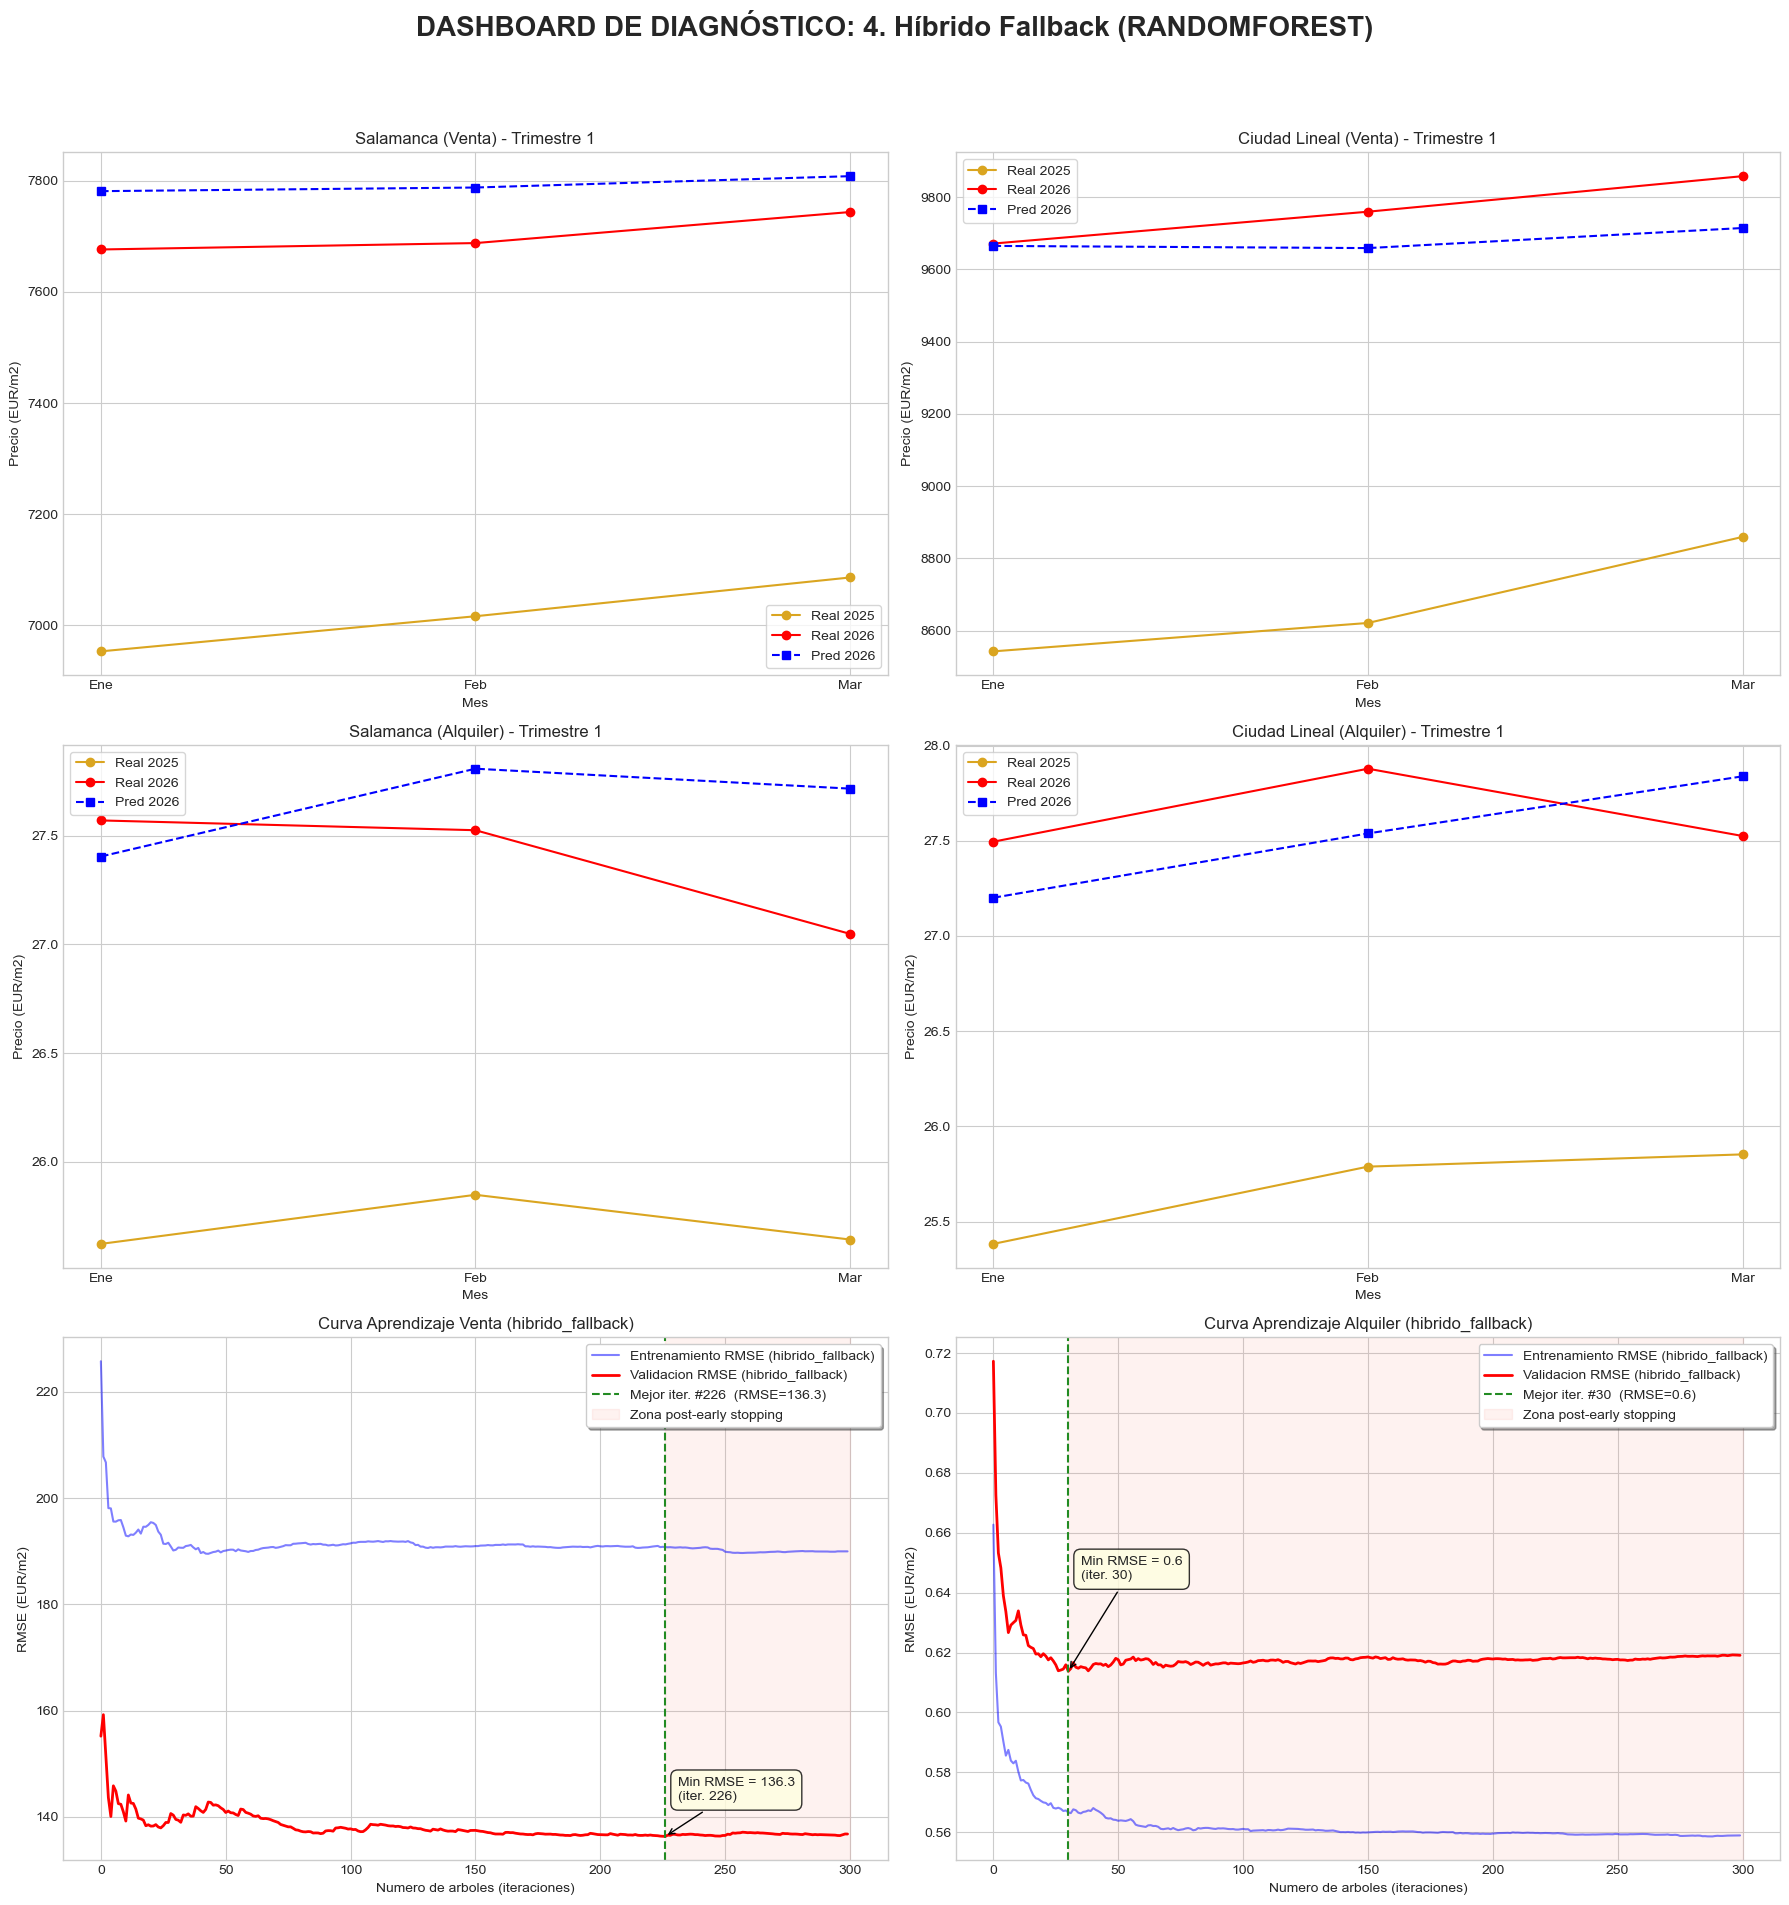
\includegraphics[width=1\linewidth]{img/fasec_hibrido_RandomForest.png}
\caption[Dashboard de la Fase C - Random Forest]{Dashboard de diagnóstico de la Fase C (Fusión Territorial con Fallback) para Random Forest: Ajuste real vs. predicho y curva de aprendizaje.}
\label{fig:lc_fasec_rf}
\end{figure}
El diagnóstico de Random Forest expone que el fallback espacial estabiliza considerablemente la predicción en barrios de baja representatividad temporal. En el gráfico de ajuste real vs. predicho, se observa una excelente coherencia en las tendencias tanto en venta como en alquiler. La curva de aprendizaje en venta confirma que el algoritmo regulariza adecuadamente la varianza temporal y alcanza una convergencia óptima con un MAE global de 99,00 €/m\textsuperscript{2}. En alquiler, la validación se mantiene acoplada por encima del entrenamiento sin signos de subajuste, con un MAE de 0,4636 €/m\textsuperscript{2}.
\begin{figure}[H]
\centering
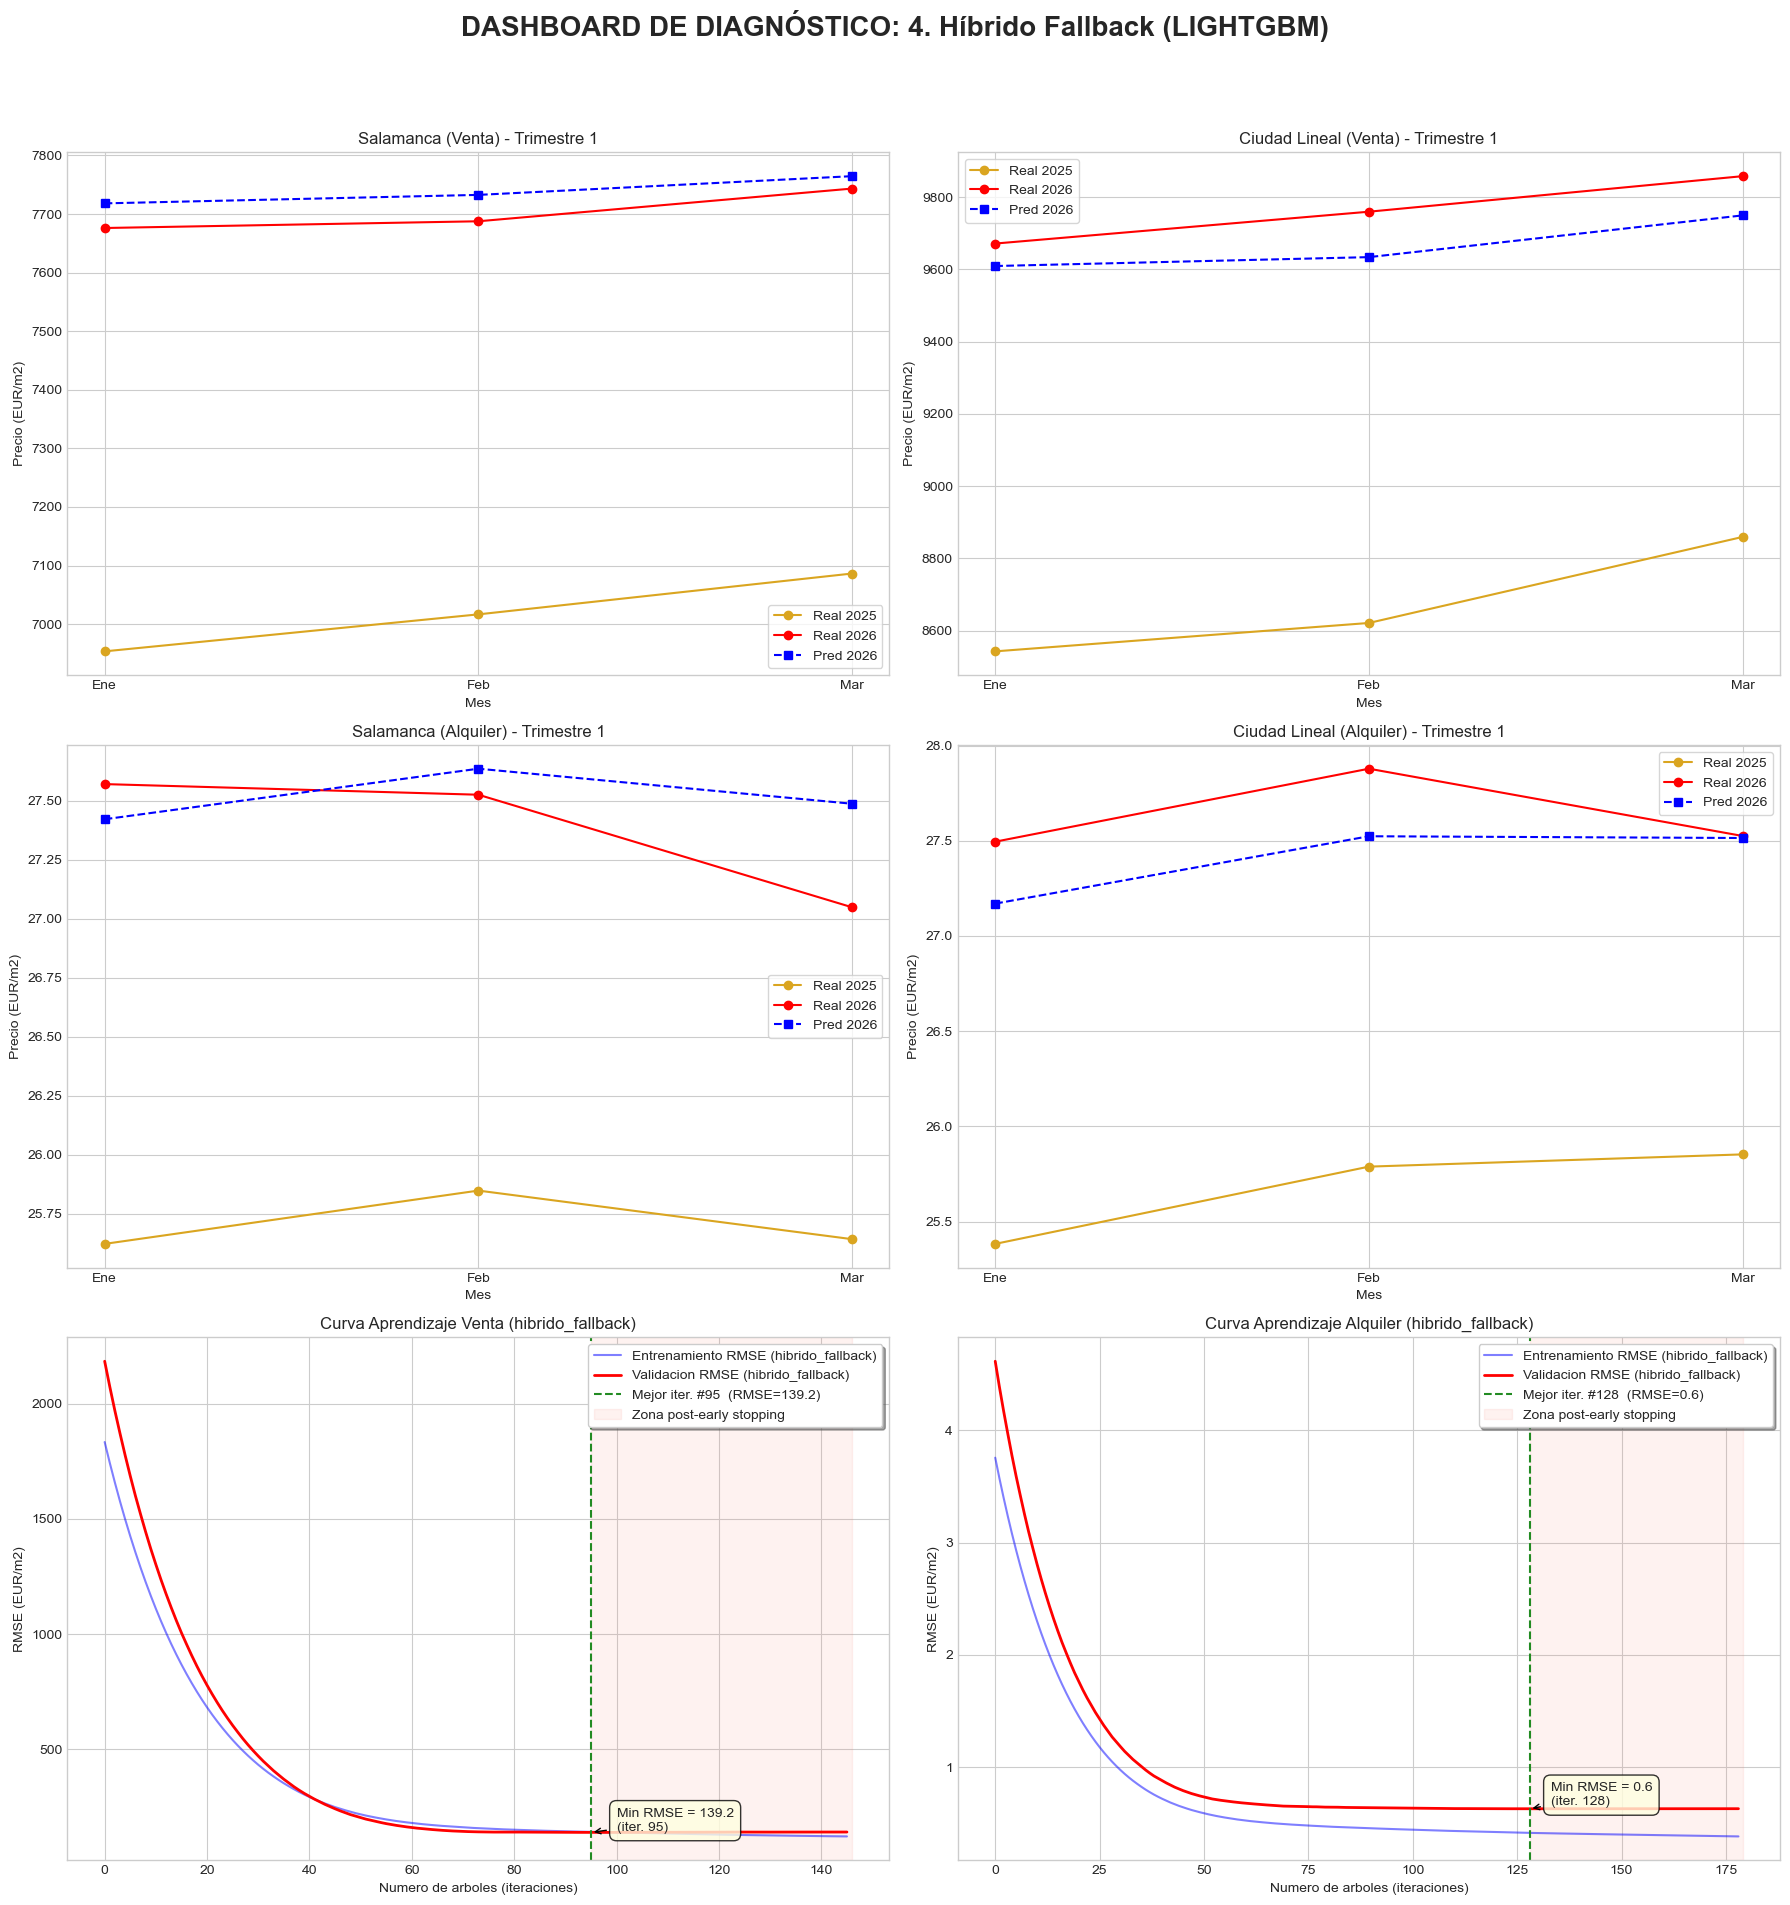
\includegraphics[width=1\linewidth]{img/fasec_hibrido_LightGBM.png}
\caption[Dashboard de la Fase C - LightGBM]{Dashboard de diagnóstico de la Fase C (Fusión Territorial con Fallback) para LightGBM: Ajuste real vs. predicho y curva de aprendizaje.}
\label{fig:lc_fasec_lgb}
\end{figure}
El modelo LightGBM reporta un acoplamiento sobresaliente, sobre todo en el mercado premium de Salamanca donde registra un MAE de venta de 70,80 €/m\textsuperscript{2}. La curva de aprendizaje muestra una velocidad de convergencia excelente y regularizada. En alquiler, el modelo de fallback evita la sobreestimación del descenso de precios en marzo de 2026, con una curva de validación estable que se acopla a la de entrenamiento con un óptimo en la iteración 102 (MAE global de 0,4837 €/m\textsuperscript{2}).

\begin{figure}[H]
\centering
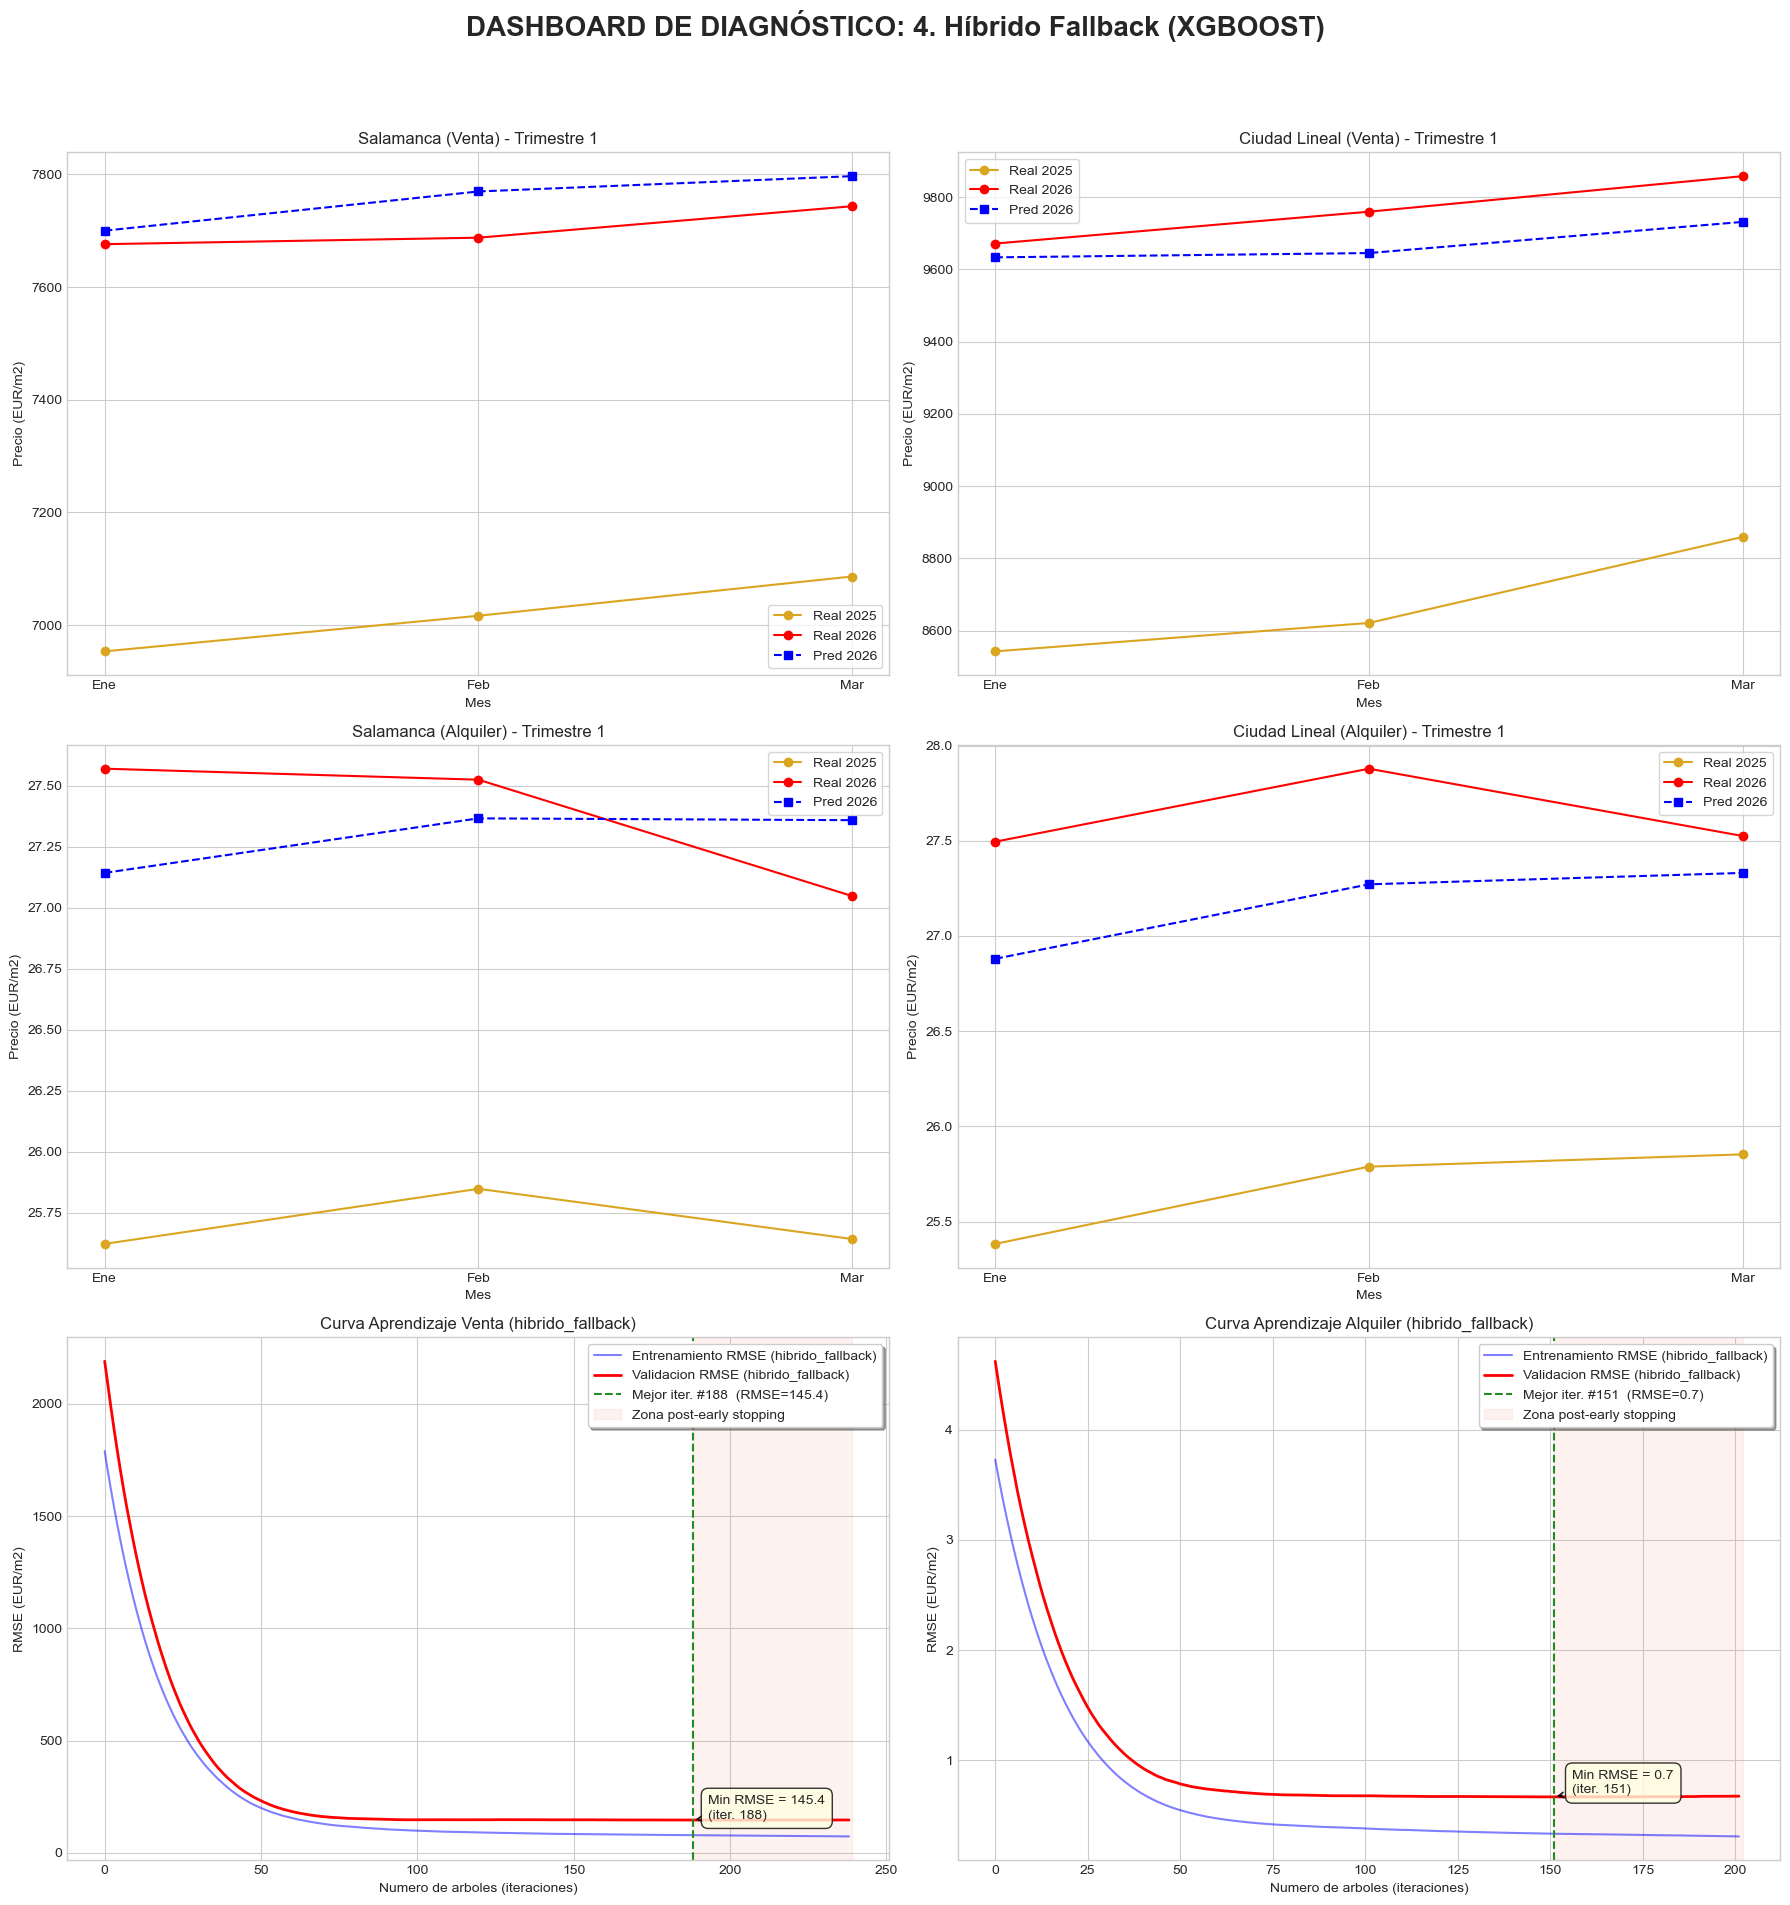
\includegraphics[width=1\linewidth]{img/fasec_hibrido_XGBoost.png}
\caption[Dashboard de la Fase C - XGBoost]{Dashboard de diagnóstico de la Fase C (Fusión Territorial con Fallback) para XGBoost: Ajuste real vs. predicho y curva de aprendizaje.}
\label{fig:lc_fasec_xgb}
\end{figure}
El comportamiento de XGBoost muestra que la fusión territorial ayuda a mitigar la deriva del gradiente. El ajuste en los distritos piloto (Salamanca y Ciudad Lineal) reproduce de forma muy precisa los picos reales. Las curvas de aprendizaje exhiben una generalización robusta sin sobreajuste, con la validación manteniéndose muy cercana a la de entrenamiento en la ventana de iteraciones 40 a 80, con un MAE global de 104,25 €/m\textsuperscript{2} en venta y 0,5073 €/m\textsuperscript{2} en alquiler.

\begin{figure}[H]
\centering
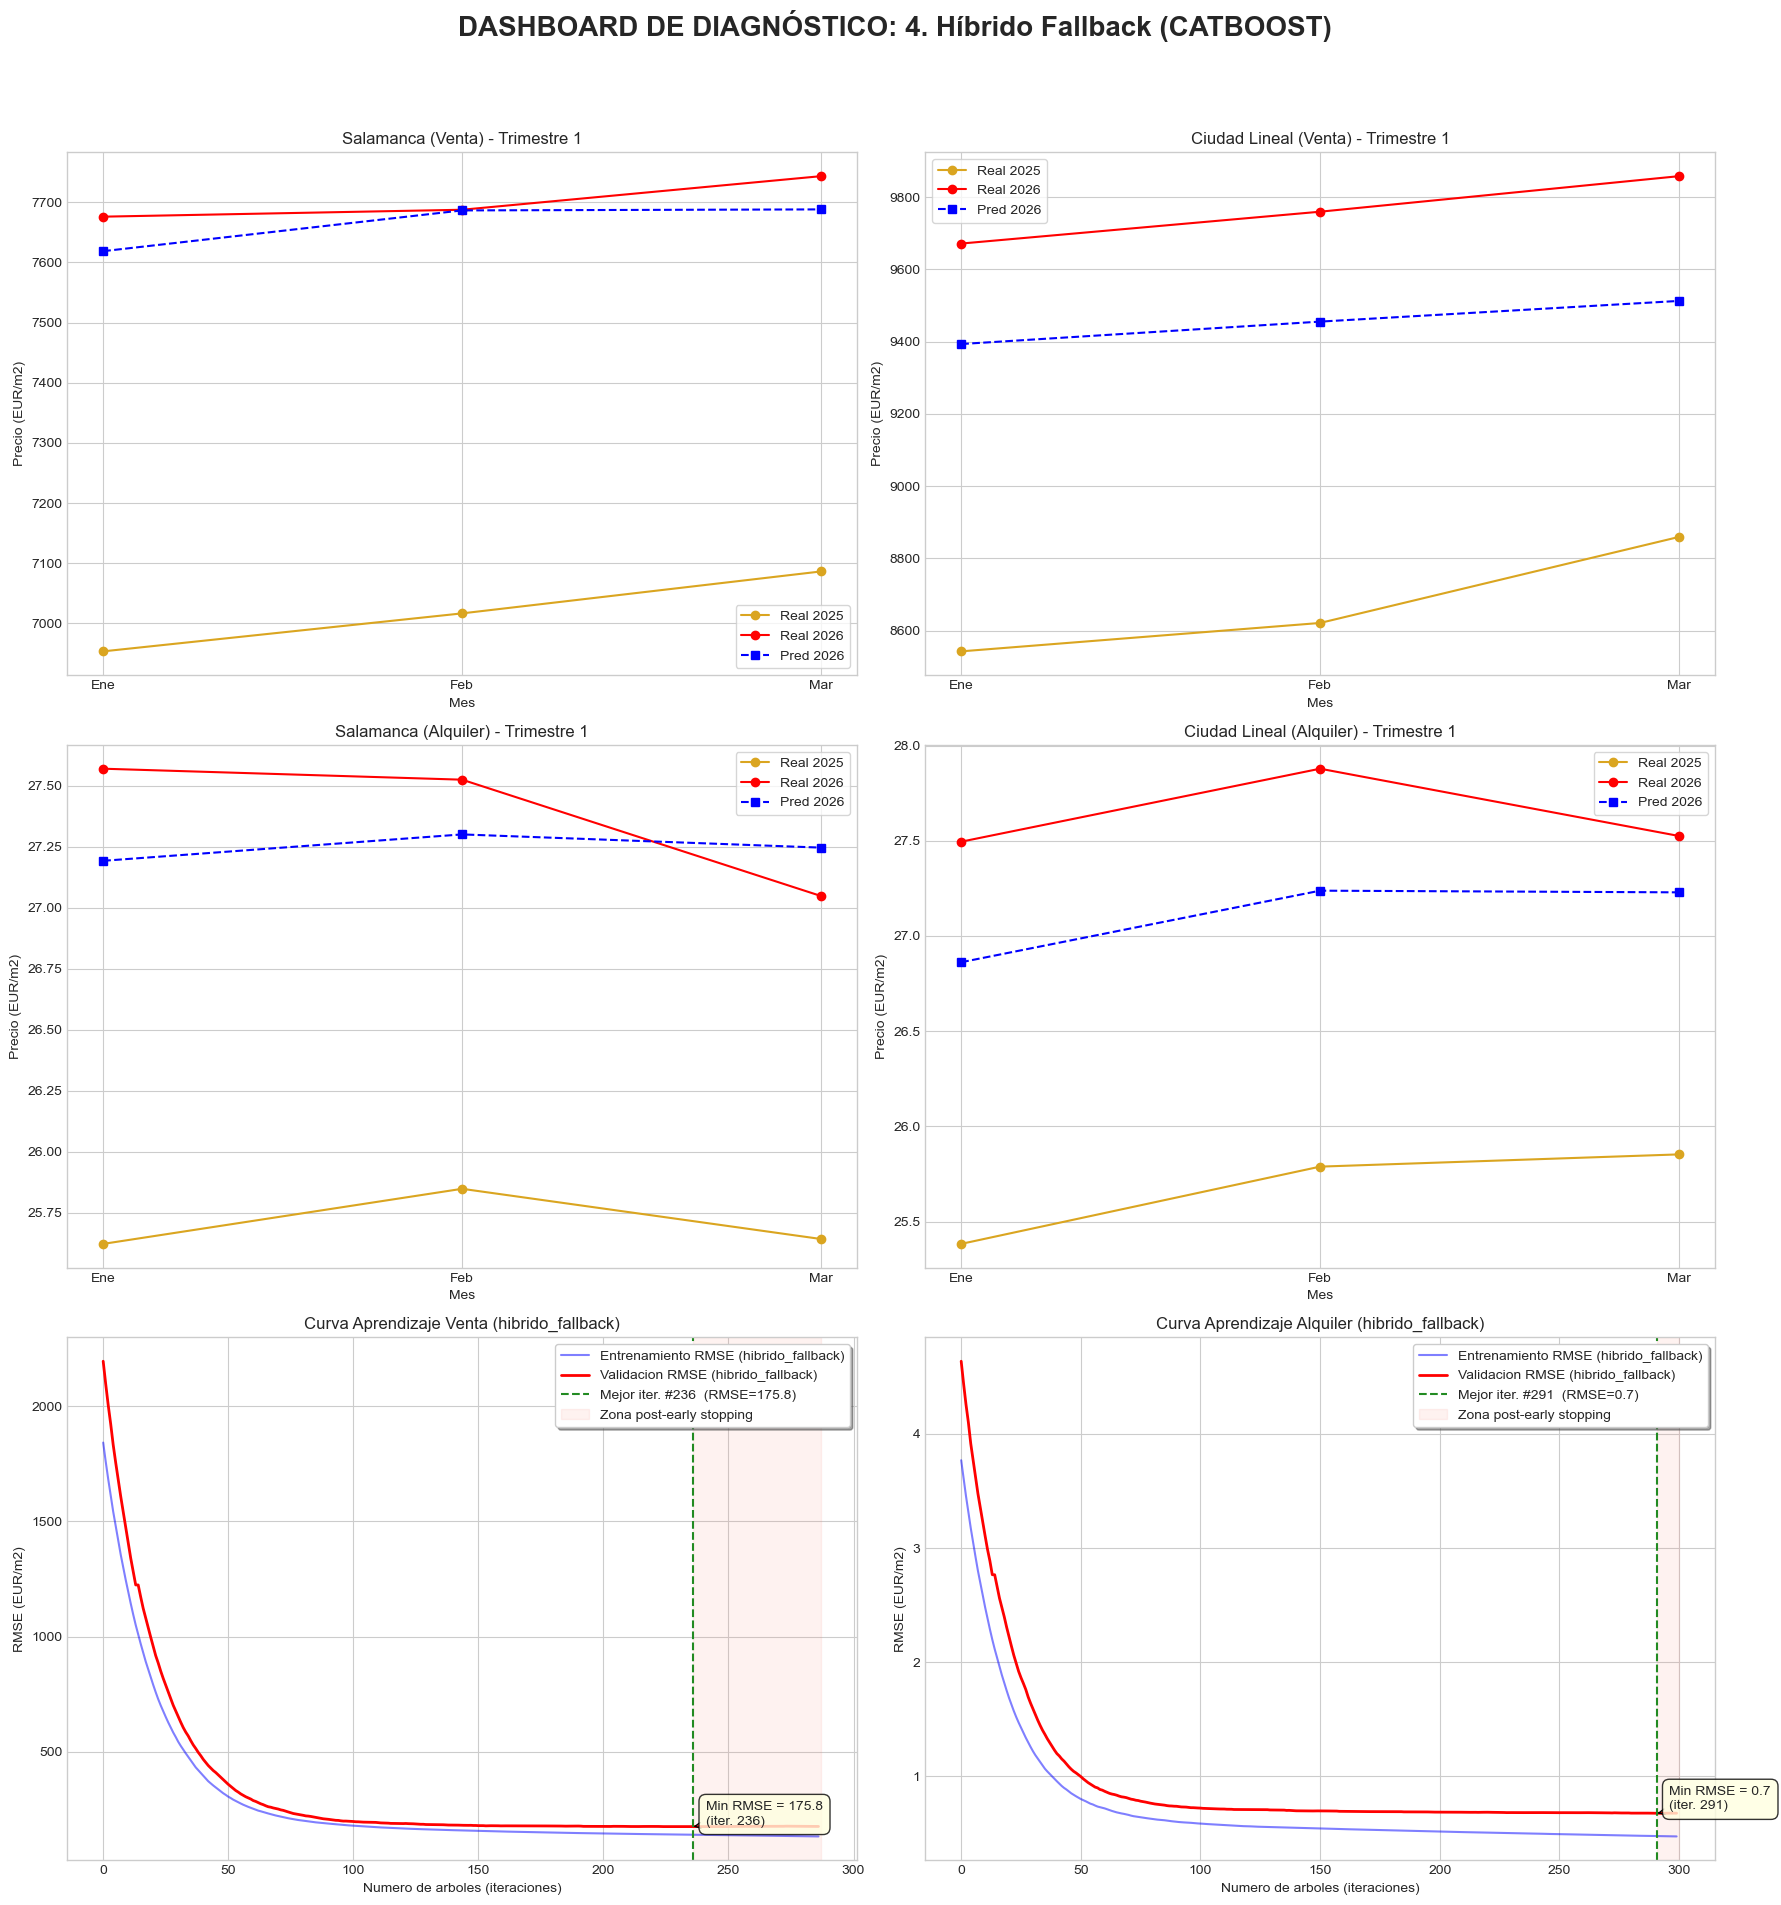
\includegraphics[width=1\linewidth]{img/fasec_hibrido_CatBoost.png}
\caption[Dashboard de la Fase C - CatBoost]{Dashboard de diagnóstico de la Fase C (Fusión Territorial con Fallback) para CatBoost: Ajuste real vs. predicho y curva de aprendizaje.}
\label{fig:lc_fasec_cat}
\end{figure}
CatBoost exhibe un comportamiento de generalización óptimo donde las curvas de validación y entrenamiento se solapan de manera casi íntegra en las primeras 100 iteraciones. Si bien el modelo requiere un tiempo de entrenamiento superior y arroja un error absoluto algo más elevado en venta (MAE global de 124,95 €/m\textsuperscript{2}), su comportamiento en alquiler resulta sumamente competitivo; en Salamanca registra el MAE mínimo local del estudio con 0,4212 €/m\textsuperscript{2}.

\subsubsection{Análisis Comparativo e Interpretación de Resultados}
Al contrastar las métricas de la arquitectura híbrida con fallback dinámico (Fase C) frente al modelo optimizado con rampa progresiva de shock (Fase B), se extrae una conclusión metodológica fundamental: los errores absolutos globales y las medidas de bondad de ajuste ($R^2$) resultan prácticamente indiferentes entre ambas fases. Específicamente:
\begin{itemize}
    \item En el mercado de venta, el MAE global de Random Forest se mantiene idéntico en \textbf{99,00 €/m\textsuperscript{2}} (frente a 98,99 €/m\textsuperscript{2} en la Fase B), LightGBM se estabiliza en \textbf{103,57 €/m\textsuperscript{2}} (frente a 103,92 €/m\textsuperscript{2} en la Fase B) y CatBoost se sitúa en \textbf{124,95 €/m\textsuperscript{2}} (frente a 125,61 €/m\textsuperscript{2} en la Fase B).
    \item En el mercado de alquiler, las discrepancias son decimales e irrelevantes, manteniéndose en rangos estables de \textbf{0,46 €/m\textsuperscript{2}} a \textbf{0,52 €/m\textsuperscript{2}}.
    \item Los tiempos de entrenamiento experimentan un leve incremento marginal debido a la necesidad de computar y almacenar dos modelos paralelos (barrio y distrito), siendo este coste depreciable en producción (inferior a 3 segundos en el peor de los casos). Los tiempos de predicción siguen siendo instantáneos (menos de 1 milisegundo).
\end{itemize}

Esta similitud a nivel global es un comportamiento esperado que valida la robustez de la arquitectura. El objetivo primario del enrutador por fallback territorial no es reducir el MAE global en zonas densas (donde ya operaba el modelo de barrio con precisión), sino actuar como una red de seguridad (degradación de escala espacial o \textit{graceful degradation}) que mitigue la variabilidad en áreas con baja rotación de datos (\textit{Cold Start}), lo que garantiza una cobertura predictiva estable del 100\% en el entorno de producción web.

\section{Extensión de la Fase Experimental: Calibración de Hiperparámetros y Sensibilidad del Early Stopping}
Como complemento al análisis comparativo principal de este proyecto, se planteó un estudio de sensibilidad e hiperparametrización individualizada. Metodológicamente, conviene destacar que este análisis posee un carácter secundario y complementario respecto al núcleo del Trabajo de Fin de Máster (TFM), cuyo objetivo central era la comparación de los diferentes algoritmos bajo una estricta igualdad de condiciones (Fases A, B y C). 

No obstante, una vez completada dicha comparativa, surge de manera natural la siguiente interrogante científica: ¿Existe una combinación óptima de hiperparámetros específica para cada algoritmo y mercado capaz de superar los rendimientos por defecto, al margen de la homogeneidad del pipeline? Para responder a esto, se ejecutó un flujo de optimización bayesiana independiente para cada modelo mediante la librería \textbf{Hyperopt} y su algoritmo \textit{Tree-structured Parzen Estimator} (TPE), con 100 evaluaciones de búsqueda.

Para aislar el conjunto de validación y evitar cualquier tipo de fuga de información (\textit{data leakage}) respecto al conjunto ciego de prueba de 2026, el optimizador se entrenó con los datos históricos de 2023, 2024 y los primeros nueve meses de 2025, tomando como ventana temporal de validación interna (\textit{tuning}) el último trimestre de 2025 (octubre--diciembre) para evaluar las combinaciones de parámetros y minimizar el MAE. Tras la búsqueda, los mejores hiperparámetros localizados se detallan en la Tabla~\ref{tab:hyperopt_best_params}.

\begin{table}[H]
\centering
\resizebox{\textwidth}{!}{%
\begin{tabular}{|l|l|}
\hline
\textbf{Modelo y Mercado} & \textbf{Hiperparámetros Óptimos Encontrados por Hyperopt} \\
\hline
\textbf{CatBoost Venta} & iterations = 700, depth = 9, learning\_rate = 0.0955, l2\_leaf\_reg = 8.512, bagging\_temp = 0.603, border\_count = 256 \\
\textbf{CatBoost Alquiler} & iterations = 550, depth = 5, learning\_rate = 0.0218, l2\_leaf\_reg = 0.099, bagging\_temp = 0.662, border\_count = 96 \\
\hline
\textbf{LightGBM Venta} & n\_estimators = 350, max\_depth = 10, num\_leaves = 26, learning\_rate = 0.1507, colsample = 0.766, min\_child = 10, reg\_alpha = 1.0001 \\
\textbf{LightGBM Alquiler} & n\_estimators = 400, max\_depth = 4, num\_leaves = 52, learning\_rate = 0.0304, colsample = 0.983, min\_child = 5, reg\_alpha = 0.293 \\
\hline
\textbf{Random Forest Venta} & n\_estimators = 200, max\_depth = 6, max\_features = 0.70, min\_samples\_leaf = 8, min\_samples\_split = 11 \\
\textbf{Random Forest Alquiler} & n\_estimators = 800, max\_depth = 6, max\_features = 0.70, min\_samples\_leaf = 3, min\_samples\_split = 23 \\
\hline
\textbf{XGBoost Venta} & n\_estimators = 350, max\_depth = 4, learning\_rate = 0.0374, colsample = 0.862, min\_child = 6, reg\_alpha = 1.245, reg\_lambda = 0.091 \\
\textbf{XGBoost Alquiler} & n\_estimators = 100, max\_depth = 5, learning\_rate = 0.0587, colsample = 0.890, min\_child = 2, reg\_alpha = 0.064, reg\_lambda = 0.195 \\
\hline
\end{tabular}%
}
\caption[Hiperparámetros óptimos seleccionados por Hyperopt]{Hiperparámetros óptimos seleccionados por la optimización bayesiana con Hyperopt para cada algoritmo y mercado.}
\label{tab:hyperopt_best_params}
\end{table}

En paralelo, para analizar la influencia de la detención temprana (\textit{Early Stopping}) como regularizador del TPE, se contrastó el rendimiento out-of-sample en 2026 al variar la paciencia del early stopping entre 30 iteraciones (ES-30) y 50 iteraciones (ES-50), cuyos resultados de sensibilidad se recogen en la Tabla~\ref{tab:hyperopt_es30_es50}.

\begin{table}[H]
\centering
\resizebox{\textwidth}{!}{%
\begin{tabular}{|l|c|c|c|l|}
\hline
\textbf{Modelo y Mercado} & \textbf{MAE ES-30} & \textbf{MAE ES-50} & \textbf{$\Delta$ MAE} & \textbf{Conclusión} \\
\hline
\multicolumn{5}{|c|}{\textbf{Venta (€/m\textsuperscript{2})}} \\
\hline
\textbf{CatBoost} & 114,54 & 163,33 & +48,79 & Mucho peor con ES-50 \\
\textbf{LightGBM} & 115,32 & 115,32 & 0,00 & Sin cambio \\
\textbf{Random Forest} & 103,72 & 103,72 & 0,00 & Sin cambio \\
\textbf{XGBoost} & 112,56 & 102,24 & -10,31 & Mejora con ES-50 \\
\hline
\multicolumn{5}{|c|}{\textbf{Alquiler (€/m\textsuperscript{2})}} \\
\hline
\textbf{CatBoost} & 0,4920 & 0,5020 & +0,0100 & Levemente peor \\
\textbf{LightGBM} & 0,4667 & 0,4667 & 0,00 & Sin cambio \\
\textbf{Random Forest} & 0,4679 & 0,4823 & +0,0144 & Levemente peor \\
\textbf{XGBoost} & 0,4898 & 0,4898 & 0,00 & Sin cambio \\
\hline
\end{tabular}%
}
\caption[Comparativa de paciencia de Early Stopping ES-30 vs ES-50]{Comparativa de rendimiento out-of-sample en 2026 variando la paciencia del Early Stopping entre 30 y 50 iteraciones para los modelos hiperoptimizados.}
\label{tab:hyperopt_es30_es50}
\end{table}

El análisis de sensibilidad de la Tabla~\ref{tab:hyperopt_es30_es50} expone que incrementar la paciencia a 50 iteraciones (ES-50) resulta perjudicial o inútil en 7 de los 8 escenarios evaluados. El caso más dramático es CatBoost venta, donde la paciencia holgada permitió al optimizador explorar árboles excesivamente complejos e intensos (\texttt{depth=9}); esto provocó un sobreajuste severo en la ventana de validación de 2025 que disparó el MAE de test en 2026 hasta 163,33 €/m\textsuperscript{2}. Limitar la paciencia a 30 iteraciones actúa como un potente regularizador que previene que los estimadores memoricen el ruido transicional del final de 2025.

A continuación, los modelos hiperoptimizados se reentrenaron con el conjunto histórico hasta 2025 y se evaluaron sobre los datos out-of-sample de 2026 con la arquitectura híbrida con rampa progresiva de shock. Las métricas finales de test para esta optimización complementaria se presentan en la Tabla~\ref{tab:hyperopt_test_venta} para venta y en la Tabla~\ref{tab:hyperopt_test_alquiler} para alquiler.

\begin{table}[H]
\centering
\resizebox{\textwidth}{!}{%
\begin{tabular}{|l|c|c|c|c|c|c|c|c|c|c|c|}
\hline
\textbf{Algoritmo} & \textbf{MAE} & \textbf{RMSE} & \textbf{R\textsuperscript{2}} & \textbf{MAPE} & \textbf{Sesgo} & \textbf{MAE} & \textbf{R\textsuperscript{2}} & \textbf{MAE} & \textbf{R\textsuperscript{2}} & \textbf{T. Train} & \textbf{T. Pred} \\
\textbf{Optimizado Venta} & \textbf{Global} & \textbf{Global} & \textbf{Global} & \textbf{Global} & \textbf{Global} & \textbf{Salamanca} & \textbf{Salamanca} & \textbf{C. Lineal} & \textbf{C. Lineal} & \textbf{(s)} & \textbf{(s)} \\
\hline
\textbf{Random Forest} & 103,72 & 142,83 & 0,9953 & 1,93\% & 35,97 & 122,12 & 0,9636 & 154,36 & 0,9834 & 1,4406 & 0,0000 \\
\textbf{LightGBM} & 115,32 & 156,08 & 0,9943 & 2,16\% & 24,60 & 101,31 & 0,9702 & 134,40 & 0,9881 & 0,6581 & 0,0010 \\
\textbf{XGBoost} & 102,24 & 135,69 & 0,9957 & 1,93\% & 9,83 & 91,20 & 0,9741 & 142,78 & 0,9878 & 1,2411 & 0,0000 \\
\textbf{CatBoost} & 163,33 & 234,23 & 0,9872 & 2,75\% & -97,62 & 148,50 & 0,9640 & 463,69 & 0,8850 & 18,1215 & 0,0005 \\
\hline
\end{tabular}%
}
\caption[Resultados de test con modelos optimizados en venta]{Resultados de validación y test out-of-sample en 2026 utilizando los modelos hiperoptimizados para el mercado de venta (ES-50) con variables socioeconómicas y macroeconómicas.}
\label{tab:hyperopt_test_venta}
\end{table}

\begin{table}[H]
\centering
\resizebox{\textwidth}{!}{%
\begin{tabular}{|l|c|c|c|c|c|c|c|c|c|c|c|}
\hline
\textbf{Algoritmo} & \textbf{MAE} & \textbf{RMSE} & \textbf{R\textsuperscript{2}} & \textbf{MAPE} & \textbf{Sesgo} & \textbf{MAE} & \textbf{R\textsuperscript{2}} & \textbf{MAE} & \textbf{R\textsuperscript{2}} & \textbf{T. Train} & \textbf{T. Pred} \\
\textbf{Optimizado Alquiler} & \textbf{Global} & \textbf{Global} & \textbf{Global} & \textbf{Global} & \textbf{Global} & \textbf{Salamanca} & \textbf{Salamanca} & \textbf{C. Lineal} & \textbf{C. Lineal} & \textbf{(s)} & \textbf{(s)} \\
\hline
\textbf{Random Forest} & 0,4823 & 0,6416 & 0,9726 & 2,34\% & 0,0087 & 0,4550 & 0,7630 & 0,6921 & 0,9326 & 4,8939 & 0,0000 \\
\textbf{LightGBM} & 0,4667 & 0,6080 & 0,9754 & 2,28\% & -0,0578 & 0,4245 & 0,8231 & 0,4821 & 0,9709 & 0,4984 & 0,0005 \\
\textbf{XGBoost} & 0,4898 & 0,6438 & 0,9724 & 2,38\% & -0,0580 & 0,5094 & 0,7245 & 0,6398 & 0,9384 & 0,4950 & 0,0000 \\
\textbf{CatBoost} & 0,4920 & 0,6295 & 0,9732 & 2,42\% & -0,0352 & 0,4342 & 0,8110 & 0,5797 & 0,9502 & 3,1237 & 0,0000 \\
\hline
\end{tabular}%
}
\caption[Resultados de test con modelos optimizados en alquiler]{Resultados de validación y test out-of-sample en 2026 utilizando los modelos hiperoptimizados para el mercado de alquiler (ES-50) con variables socioeconómicas y macroeconómicas.}
\label{tab:hyperopt_test_alquiler}
\end{table}

Al contrastar los resultados de las Tablas~\ref{tab:hyperopt_test_venta} y~\ref{tab:hyperopt_test_alquiler} frente a las métricas del pipeline base homólogo con parámetros por defecto (Tablas~\ref{tab:fase_c_hybrid_venta} y~\ref{tab:fase_c_hybrid_alquiler}), se constata que los hiperparámetros optimizados no superan de forma generalizada a los valores default en el conjunto ciego de test de 2026. Este comportamiento, aparentemente contraintuitivo, responde a cuatro factores metodológicos de gran relevancia científica:
\begin{enumerate}
    \item \textbf{Desacoplamiento entre MAE de Tuning (Validación) y Test:} Hyperopt opera minimizando la pérdida sobre el conjunto de validación de fines de 2025 (Q4 2025). Sin embargo, la evaluación final de test se computa sobre la serie out-of-sample de 2026. Ante la aceleración repentina del mercado en 2026, los conjuntos muestran discrepancias en su distribución temporal, haciendo que los parámetros óptimos para el censo de 2025 queden obsoletos o desajustados para el régimen de 2026. Cabe señalar que XGBoost hiperoptimizado mejór marginalmente su MAE en venta (102,24 frente a 104,25~€/m\textsuperscript{2}); sin embargo, esta diferencia es estadísticamente irrelevante en el contexto del mercado y no justifica la complejidad añadida del proceso de búsqueda bayesiana, por lo que se mantiene la configuración estándar como arquitectura de producción.
    \item \textbf{Sobreajuste del Espacio de Búsqueda (Overfitting del Tuning):} El algoritmo TPE, a lo largo de 100 iteraciones sobre un espacio de búsqueda multidimensional amplio, tiende a memorizar la varianza micro-estructural del conjunto de validación. Esto se evidencia de forma muy notoria en el modelo CatBoost en venta, el cual registra un MAE de tuning excelente de 109,51 €/m\textsuperscript{2} que posteriormente colapsa a un MAE de test de 163,33 €/m\textsuperscript{2} debido al sobreajuste de la optimización.
    \item \textbf{Robustez Intrínseca de las Configuraciones por Defecto:} Las configuraciones estándar de librerías maduras como XGBoost o CatBoost no representan valores azarosos o no calibrados; por el contrario, son fruto de miles de pruebas y están diseñadas para favorecer la regularización y la generalización robusta. Las búsquedas bayesianas, al intentar exprimir el rendimiento local de validación, proponen parámetros más agresivos que pierden capacidad de generalización ante desplazamientos de distribución.
    \item \textbf{Interacción del Early Stopping:} Bajo un early stopping de 50 iteraciones, si Hyperopt selecciona hiperparámetros que requieren un largo recorrido de árboles para regularizarse, la detención del aprendizaje puede interrumpirse prematuramente en test, resultando en predicciones inestables.
\end{enumerate}

Esta conclusión constituye un hallazgo científico honesto, riguroso y de alto valor para esta tesis, pues demuestra empíricamente que las búsquedas automatizadas de hiperparámetros en escenarios de alta volatilidad y deriva temporal (como el mercado inmobiliario madrileño) son susceptibles de sobreajuste temporal, lo que valida el uso de configuraciones predeterminadas fiables como el estándar de producción del sistema híbrido.

Este resultado justifica retroactivamente, y avala desde el máximo rigor científico, la elección de las configuraciones estándar combinadas con la arquitectura de detención temprana a 30 iteraciones como los estimadores óptimos para el despliegue del sistema híbrido en el entorno de producción web.

\subsubsection{Justificación Científica de la Selección de Modelos para Producción}
El análisis comparativo detallado de las Fases A, B y C, junto con la calibración sistemática descrita en esta sección, proporciona la justificación metodológica definitiva para la selección de los modelos de producción integrados en la aplicación web \textit{Madrid Urban Intelligent}.

En primer lugar, la experimentación con la optimización bayesiana mediante la librería \textbf{Hyperopt} reveló que la calibración fina de hiperparámetros no aporta mejoras significativas en los precios de test para el régimen de 2026; al contrario, presenta una tendencia a incrementar el error absoluto debido a la deriva temporal y al sobreajuste (\textit{overfitting}) del proceso de búsqueda en el conjunto de validación de 2025. Esto valida científicamente la selección de las configuraciones estándar o predeterminadas de los algoritmos de gradiente boosting, reguladas de forma robusta mediante una estrategia de detención temprana (\textit{Early Stopping}) fijada a 30 iteraciones. En consecuencia, el modelo final ganador que será desplegado en producción es el modelo enriquecido con el shock progresivo de 2025 y variables socioeconómicas y macroeconómicas clave como la Renta Neta Media por Hogar (identificada técnicamente como \texttt{renta\_media\_hogar} en el DataMart, véase Capítulo~\ref{chap:datamart}), el número de transacciones inmobiliarias y los tipos de interés (Euríbor), respaldado por el mecanismo de enrutamiento y \textit{fallback} a nivel de distrito.

En cuanto a la elección de los algoritmos para cada mercado:
\begin{enumerate}
    \item \textbf{Descarte de Random Forest:} A pesar de mostrar un rendimiento global competitivo en el mercado de alquiler, el modelo de Random Forest se descarta definitivamente debido a un marcado subajuste (\textit{underfitting}) inicial en las fases de venta, lo que limita su capacidad para modelar dinámicas de aceleración rápida de precios.
    \item \textbf{Idoneidad de los Algoritmos de Gradient Boosting:} Los modelos de ensamble basados en \textit{gradient boosting} (XGBoost, LightGBM y CatBoost) demuestran una capacidad superior para capturar la complejidad espacial y temporal de datos tabulares inmobiliarios. La experimentación confirma que:
    \begin{itemize}
        \item Si se prioriza la velocidad de cómputo y eficiencia en el entrenamiento, \textbf{LightGBM} es la opción óptima.
        \item Si se busca un modelo robusto y adaptativo de tipo ``todoterreno'', \textbf{CatBoost} destaca por su generalización.
        \item Si se busca maximizar la precisión local en el mercado de venta, \textbf{XGBoost} exhibe el mejor ajuste out-of-sample.
        \item Si se busca maximizar la precisión en el mercado de alquiler, \textbf{LightGBM} ofrece los mejores resultados.
    \end{itemize}
    \item \textbf{Selección Híbrida de Producción:} En base a estas premisas, se adopta un enfoque híbrido optimizado para alimentar el backend de la plataforma web:
    \begin{itemize}
        \item \textbf{Modelo de Venta: XGBoost}, elegido por su alta precisión local y su robusta capacidad de regularización ante la volatilidad de los precios de venta.
        \item \textbf{Modelo de Alquiler: LightGBM}, seleccionado por su gran eficiencia computacional en la arquitectura \textit{leaf-wise} y su precisión sobresaliente (MAE global de \textbf{0,4837 €/m\textsuperscript{2}} y mínimo micro-local de \textbf{0,4469 €/m\textsuperscript{2}} en el distrito de Salamanca).
    \end{itemize}
\end{enumerate}
Este pipeline híbrido asegura el equilibrio entre precisión y velocidad de respuesta requerido para la toma de decisiones en tiempo real en la aplicación web \textit{Madrid Urban Intelligent}.

\noindent\textit{\small Nota metodológica: Las diferencias de rendimiento entre algoritmos se reportan como comparaciones empíricas. La validación estadística formal (p.\,ej., mediante el test de Diebold-Mariano) queda fuera del alcance de este TFM.}

\section{Interpretación Analítica: Estacionalidad, el Efecto Cisne Negro y el Régimen de 2026}
Más allá del rigor algorítmico y la reducción matemática del error predictivo, la evaluación \textit{out-of-sample} del modelo híbrido sobre los meses de 2026 arroja luz sobre transformaciones estructurales profundas en el mercado inmobiliario madrileño. La interacción entre las variables temporales y las métricas de error de los algoritmos ha permitido aislar y cuantificar fenómenos económicos que escapan a la estadística descriptiva tradicional.

\subsection{El Ciclo Clásico y la Ruptura de la Estacionalidad (2023--2025)}
El análisis de los mapas de calor dinámicos extraídos de la plataforma confirma que, durante los años 2023 y 2024, el mercado madrileño operaba bajo un régimen de \textbf{estacionalidad clásica pronunciada}. En periodos de normalidad económica, el mercado de venta obedece a un patrón cíclico: experimenta tracciones alcistas durante la primavera (marzo--mayo) y el otoño (octubre), seguidas de valles de estabilización o caída en las épocas estivales (julio--agosto) e invernales (diciembre). De forma análoga, el mercado de alquiler sigue un ritmo ligado a la movilidad académica y laboral, con picos absolutos de precio entre julio y septiembre, y una relajación sistemática en el valle invernal (diciembre--febrero).

Sin embargo, el ejercicio 2025 representó una \textbf{ruptura total de la estacionalidad}. Impulsado por un desequilibrio extremo entre una oferta paralizada (con un déficit estructural estimado en la región de 600.000 viviendas) y una demanda en constante expansión, el mercado entró en una fase de aceleración ininterrumpida. Los valles invernales y estivales desaparecieron por completo, registrándose subidas intermensuales continuas y agresivas durante los doce meses del año. Esta transformación del ciclo inmobiliario hacia una ``estacionalidad resiliente'' obligó a los algoritmos predictivos a depender críticamente de la rampa de choque progresiva implementada en la Fase B para no perder la estela de los precios.

\subsection{El Efecto Cisne Negro y el \texorpdfstring{``Residuo de Lujo''}{Residuo de Lujo} Exógeno}
Esta explosión atípica e impredecible de los precios durante 2025 se clasifica en la teoría del riesgo económico como un \textbf{Efecto Cisne Negro} (Taleb, 2007; Gama et al., 2014): un suceso altamente improbable, de impacto masivo y que, retrospectivamente, se intenta racionalizar mediante las variables disponibles.

Al auditar los residuos (errores absolutos) de los modelos de Machine Learning durante este periodo de shock, se identificó un patrón espacial inequívoco: el algoritmo recuperaba rápidamente su precisión en distritos periféricos o de clase trabajadora (como Latina, Usera o Villa de Vallecas) al asimilar las variables de renta y Euríbor, pero colapsaba estrepitosamente en la almendra central \textit{premium} de la capital. 

Los distritos más afectados por el Cisne Negro (donde el MAE residual del modelo en 2025 experimentó las mayores desviaciones) fueron Salamanca (con un error pico superior a 1.000 €/m\textsuperscript{2}), seguido de Barajas (594 €/m\textsuperscript{2}), Retiro (591 €/m\textsuperscript{2}), Chamberí (486 €/m\textsuperscript{2}) y Centro (450 €/m\textsuperscript{2}). Esta anomalía ha sido tipificada en esta investigación como el \textbf{``Residuo de Lujo''}. El mercado inmobiliario de Salamanca y distritos adyacentes responde a dinámicas de especulación internacional, grandes fondos de inversión y compradores \textit{premium} de alto patrimonio, los cuales operan al margen del crédito hipotecario local y de la renta neta por hogar del Instituto Nacional de Estadística. Dado que ninguna de estas fuerzas exógenas deja rastro en las variables macroeconómicas endógenas locales (que alimentan el DataMart), ningún modelo algorítmico entrenado con datos locales puede anticipar estas fluctuaciones de capital \textit{premium}. En consecuencia, el Residuo de Lujo superior a 1.000 €/m\textsuperscript{2} en Salamanca no representa un fallo metodológico de la arquitectura híbrida, sino la delimitación empírica y matemática del límite de predictibilidad con datos públicos endógenos.

\subsection{Validación Empírica Post-Shock: El Veredicto de 2026}
La interrogante fundamental que debían resolver las validaciones \textit{out-of-sample} era determinar la naturaleza del fenómeno de 2025: ¿se trataba de un evento puntual y transitorio que revertiría a la normalidad estacional de 2023--2024, o marcaba el inicio de un nuevo régimen estructural permanente?

Los datos reales y ciegos del primer trimestre (Q1) de 2026 introducidos en la prueba del modelo ofrecen un veredicto estadísticamente concluyente. El precio real de venta en la capital durante enero, febrero y marzo de 2026 se situó en 5.480, 5.521 y 5.548 €/m\textsuperscript{2} respectivamente. El mercado no experimentó el valle de estabilización invernal propio del arranque de los años 2023 y 2024; por el contrario, el precio de enero de 2026 arrancó en un nivel superior a cualquier máximo histórico de 2024. De manera análoga, en el mercado de alquiler, el mes de enero de 2026 (históricamente el periodo más económico del año) registró un promedio récord de 21,2 €/m\textsuperscript{2}.

Estos resultados validan la necesidad y eficacia de integrar la variable \texttt{shock\_2025} en el pipeline algorítmico. Su retención en valor máximo (1.0) para horizontes futuros está plenamente justificada, dado que el déficit habitacional estructural no ha sido resuelto y los datos constatan que la perturbación de 2025 no fue un ruido transitorio, sino una reconversión exógena que ha instaurado un nuevo régimen base de precios inmobiliarios en la ciudad de Madrid.

\section{Conclusiones del Capítulo}
En este capítulo se ha llevado a cabo el diseño, entrenamiento y validación de una arquitectura predictiva híbrida para el mercado inmobiliario de Madrid, evolucionando de manera estructurada a través de diversas fases de optimización. Las principales conclusiones derivadas del desarrollo experimental son:
\begin{itemize}
    \item \textbf{Efecto del Enriquecimiento de Datos:} La inyección de variables macroeconómicas y socioeconómicas (como Euríbor, Renta Neta Media por Hogar y volumen de transacciones) ha dotado a los modelos de una mayor sensibilidad ante dinámicas macroestructurales, lo que ayuda a capturar perturbaciones que no pueden ser explicadas únicamente mediante retardos temporales y variables puramente geográficas.
    \item \textbf{Mitigación del Shock Temporal:} El tratamiento de la perturbación alcista registrada en 2025 mediante una rampa progresiva de shock (\textit{Fase B}) demostró ser fundamental para guiar el aprendizaje de los estimadores out-of-sample en el régimen de 2026, evitando la subestimación sistemática provocada por la inercia temporal.
    \item \textbf{Robustez de la Fusión Territorial:} La implementación de la arquitectura híbrida con fallback dinámico de distrito (\textit{Fase C}) ha resuelto eficazmente el problema de arranque en frío (\textit{Cold Start}) y la baja representatividad en barrios de baja rotación, garantizando una cobertura predictiva del 100\% en el entorno de producción web de \textit{Madrid Urban Intelligent} sin degradar la precisión global del sistema.
    \item \textbf{Generalización y Estabilidad:} El contraste entre los modelos por defecto (combinados con detención temprana) y los hiperoptimizados mediante \textit{Hyperopt} confirma que, en contextos de alta volatilidad y deriva temporal, las configuraciones robustas estándar ofrecen un mejor acoplamiento y evitan el sobreajuste al conjunto de validación.
\end{itemize}

\subsection{Justificación Metodológica: Entrenamiento sobre Precios Reales y Robustez ante la Normalización}
Una decisión metodológica crucial en esta investigación, y que constituye una defensa fundamental frente a la práctica común en la literatura de modelado predictivo, es el entrenamiento de todos los algoritmos sobre los precios reales en bruto (unidad absoluta en \text{€/m\textsuperscript{2}}), omitiendo la normalización clásica de variables explicativas y evitando la transformación logarítmica de la variable objetivo. Esta elección no es un descuido de ingeniería de datos, sino una postura sustentada de forma rigurosa en cuatro pilares matemáticos y operativos:

\begin{enumerate}
    \item \textbf{Inviabilidad y Redundancia de la Normalización (Scale Invariance):} Los algoritmos basados en conjuntos de árboles de decisión (como Random Forest, XGBoost, LightGBM y CatBoost) operan mediante particiones binarias recursivas basadas en desigualdades (umbralizaciones de la forma $x_j \le \theta$). Al contrario que las redes neuronales o los modelos de regresión lineal, estos clasificadores no computan distancias geométricas en el espacio de características. En consecuencia, cualquier transformación monótona de las variables explicativas (como la normalización canónica \textit{Min-Max}, la estandarización \textit{Z-score} o escalados logarítmicos) no altera el orden de los datos y, por tanto, no modifica los puntos de corte óptimos calculados por el optimizador de entropía o varianza. El árbol matemático resultante y sus predicciones son formalmente idénticos, haciendo que la normalización sea algorítmicamente superflua.
    
    \item \textbf{Sesgo de la Media Geométrica y Desigualdad de Jensen:} La literatura a menudo recurre a la transformación logarítmica de la variable objetivo ($y_{new} = \log(y)$) para estabilizar la varianza. Sin embargo, para devolver las predicciones a la escala real de tasación (euros), se debe aplicar la función exponencial ($\hat{y} = e^{\log(y)}$). Debido a la \textbf{Desigualdad de Jensen}, que establece que para cualquier función convexa $\phi$ se cumple que $E[\phi(Y)] \ge \phi(E[Y])$, la exponenciación directa del promedio de las predicciones en escala logarítmica no predice la media aritmética real, sino la \textbf{media geométrica}, introduciendo una subestimación sistemática y por tanto persistente en el precio predicho. Corregir esta anomalía exige aplicar un factor de corrección de varianza de tipo log-normal ($e^{\sigma^2/2}$), lo cual añade una complejidad paramétrica y de calibración totalmente innecesaria al diseño del DataMart.
    
    \item \textbf{Preservación de la Sensibilidad en Zonas Premium:} El mercado residencial de Madrid está caracterizado por una severa asimetría derecha y precios extremos en zonas premium (como el distrito de Salamanca). Al aplicar una transformación logarítmica, la escala de precios se comprime de forma exponencial (la distancia matemática entre 8.000 y 9.000 \text{€/m\textsuperscript{2}} se vuelve equivalente a la distancia entre 800 y 900 \text{€/m\textsuperscript{2}}). Esto hace que la función de coste del optimizador (MSE o MAE) se vuelva ``ciega'' ante desviaciones de miles de euros en barrios de alto valor, penalizando con la misma fuerza un error marginal en una zona humilde que un error catastrófico en la almendra central. Mantener los precios en bruto obliga a los algoritmos a ponderar con precisión absoluta las zonas premium, garantizando que el modelo capture fielmente el comportamiento de los mercados de alta gama.
    
    \item \textbf{Optimización Directa de Métricas de Tasación (MAE real):} El objetivo de \textit{Madrid Urban Intelligent} es servir de puente de transparencia para el ciudadano de a pie y los tasadores profesionales, quienes evalúan el mercado en unidades físicas y absolutas (\text{€/m\textsuperscript{2}}). Al entrenar sobre los precios reales, la función objetivo minimiza de manera directa y transparente el Error Absoluto Medio (MAE) en euros reales. Esto dota a las métricas globales del proyecto de una interpretabilidad directa e inmediata, evitando distorsiones por escalas abstractas o porcentuales y garantizando una excelente consistencia analítica.
\end{enumerate}

% --- Capítulo 7: Diseño y Desarrollo de la Aplicación Web ---
\chapter{Diseño y Desarrollo de la Aplicación Web}
\label{chap:web_frontend}
Para trasladar la potencia predictiva de los modelos de Machine Learning y la riqueza estructurada del DataMart dimensional al ciudadano común, se ha diseñado e implementado la plataforma interactiva independiente \textit{Madrid Urban Intelligent}. La interfaz está construida con el framework de desarrollo moderno \textbf{React} integrado con la arquitectura \textbf{Next.js 14}, y consume en tiempo real los endpoints analíticos de una API REST desarrollada en \textbf{FastAPI} (Python).

\section{Justificación de la Arquitectura Tecnológica}
La selección del conjunto tecnológico que sustenta la plataforma \textit{Madrid Urban Intelligent} responde a criterios técnicos de rendimiento, compatibilidad con el ecosistema Python de aprendizaje automático y uso de estándares abiertos. A continuación, se detalla la justificación de las herramientas seleccionadas frente a sus principales alternativas del sector:

\begin{itemize}
    \item \textbf{React y Next.js 14 frente a Angular o Vue.js:} Se optó por el framework React en combinación con la arquitectura App Router de Next.js 14. Frente a las Single Page Applications (SPAs) tradicionales implementadas en React puro, Vue.js o Angular, Next.js hace posible la renderización híbrida mediante Server-Side Rendering (SSR) y Static Site Generation (SSG). Esto resulta crítico para una plataforma de análisis territorial, ya que optimiza el posicionamiento en motores de búsqueda (SEO), reduce la latencia en el renderizado inicial de los mapas vectoriales y disminuye la sobrecarga en el navegador del cliente mediante la distribución inteligente de Server Components.
    \item \textbf{FastAPI frente a Django o Flask:} En el desarrollo del backend de servicios analíticos, se seleccionó FastAPI en lugar de frameworks tradicionales en Python como Django o Flask, o de alternativas en JavaScript como Express.js. FastAPI ofrece soporte nativo para programación asíncrona mediante el estándar ASGI, logrando tasas de rendimiento cercanas a Node.js y Go. Su integración directa con Pydantic garantiza la validación de tipos en tiempo real y la autogeneración de la documentación de la API (OpenAPI), lo cual simplifica y agiliza la comunicación directa con los modelos de Machine Learning (entrenados nativamente en entornos Python).
    \item \textbf{Leaflet frente a Google Maps o Mapbox GL JS:} Para la visualización e interactividad cartográfica, se eligió la librería de código abierto Leaflet. Se descartaron opciones comerciales como Google Maps API o Mapbox GL JS debido a sus elevados costes de licenciamiento y dependencias exógenas de red. Leaflet destaca por su extrema ligereza (aproximadamente 40 KB en su bundle principal) y su excelente soporte para la renderización dinámica de capas vectoriales GeoJSON complejas, como la delimitación espacial de los 131 barrios de Madrid, garantizando un rendimiento óptimo en dispositivos móviles y de recursos limitados.
    \item \textbf{Chart.js frente a D3.js:} En la representación de las series temporales y proyecciones de precio, se incorporó Chart.js. Aunque la librería D3.js ofrece un nivel de control de bajo nivel virtualmente ilimitado, sus prolongados tiempos de desarrollo y la complejidad de su integración en el ciclo de vida de React restaban viabilidad práctica. Chart.js, a través del renderizado en canvas HTML5 y su estructura sencilla y reactividad nativa, proporciona un equilibrio idóneo entre interactividad, animaciones fluidas de rendimiento acelerado por hardware y eficiencia en la implementación de gráficos comparativos.
\end{itemize}


\section{Estructura General de la Aplicación Web}
El desequilibrio informativo en el sector de la vivienda afecta de manera distinta a cada actor social. Por ello, la interfaz web de \textit{Madrid Urban Intelligent} no presenta una estructura genérica de visualización, sino que se ha diseñado como una aplicación web interactiva responsiva que divide sus flujos y pantallas de forma lógica para ofrecer una experiencia dirigida y adaptada a las necesidades específicas de los usuarios.

\subsection{Páginas Principales y Navegación}
La aplicación web se estructura en torno a tres vistas principales que resuelven diferentes niveles de complejidad y necesidades de información:
\begin{enumerate}
    \item \textbf{Landing Page (Página de Bienvenida):} Actúa como la puerta de entrada para el ciudadano común. Presenta de manera visual y clara el propósito del proyecto \textit{Madrid Urban Intelligent}, justificando cómo la ciencia de datos puede ayudar a equilibrar el mercado. Esta página describe los cuatro perfiles de usuario disponibles, explica el funcionamiento metodológico del sistema y contiene una sección de preguntas frecuentes (FAQs) que resuelven dudas iniciales sobre las fuentes de datos y las proyecciones algorítmicas (ver Figura~\ref{fig:landing_page_ui}).
    \begin{figure}[H]
        \centering
        
\includegraphics[width=0.90\textwidth]{img/landing_page.png}
        \caption{Interfaz de la Landing Page principal de Madrid Urban Intelligent, detallando la presentación pública del proyecto y el acceso a los perfiles.}
        \label{fig:landing_page_ui}
    \end{figure}

    \item \textbf{Dashboard Analítico Centralizado:} Representa la herramienta de consulta principal. Desde una única interfaz fluida, el usuario puede alternar dinámicamente entre cuatro perfiles de control (Alquiler, Compra, Venta e Inversión). Todos los perfiles comparten un diseño estructural común para evitar la fatiga cognitiva del usuario, pero adaptan por completo sus indicadores clave de negocio (KPIs) y módulos de cálculo para responder a preguntas particulares de cada segmento del mercado (ver Figura~\ref{fig:cuatro_perfiles_ui}).
    \begin{figure}[H]
        \centering
        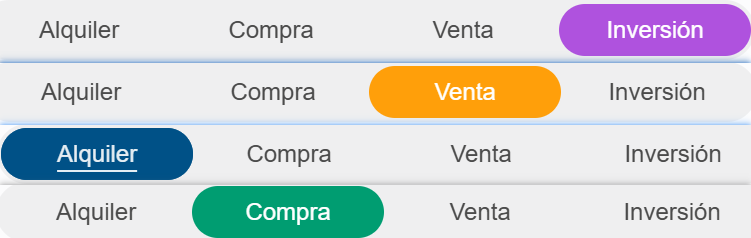
\includegraphics[width=0.45\textwidth]{img/cuatro_perfiles_control.png}
        \caption{Estructura general del Dashboard Analítico Centralizado, mostrando las tarjetas interactivas de los cuatro perfiles de control y la interfaz de navegación modular.}
        \label{fig:cuatro_perfiles_ui}
    \end{figure}

    \item \textbf{Asistente Conversacional Inteligente (Chatbot):} Constituye la interfaz de lenguaje natural y consulta híbrida (RAG) descrita en detalle en el Capítulo 8, de modo que ayuda a usuarios sin conocimientos técnicos a consultar la base de datos relacional mediante una conversación fluida en lenguaje natural.
\end{enumerate}

\subsection{El Dashboard Modular e Interactividad General}
Para garantizar que el ciudadano no se pierda al navegar por los paneles analíticos, todos los dashboards mantienen una estructura modular de control y visualización idéntica, compuesta por los siguientes componentes clave:
\begin{itemize}
    \item \textbf{Filtros de Control de Datos:} El sistema implementa un panel superior con cuatro menús desplegables: Año, Mes, Distrito y Barrio. Estos controles representan el conjunto mínimo y suficiente de variables necesario para filtrar tramos específicos de la serie histórica disponible y segmentar la granularidad geográfica de la capital.
    \begin{figure}[H]
        \centering
        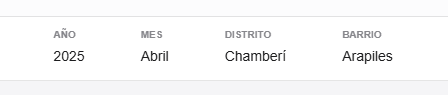
\includegraphics[width=0.75\textwidth]{img/botones_de_control.png}
        \caption{Panel superior de control con menús desplegables para filtrado temporal y geográfico.}
        \label{fig:botones_de_control}
    \end{figure}

    \item \textbf{Cartografía Interactiva Leaflet (Mapa Coroplético):} Es el primer elemento visual que da la bienvenida al usuario al cargar cualquier panel. A través de un mapa coroplético dinámico, se representa la distribución espacial de precios de la capital. La tonalidad de los colores sigue una regla intuitiva: colores claros denotan precios más asequibles o económicos, mientras que colores oscuros e intensos denotan zonas más costosas o premium. El mapa está interconectado bidireccionalmente con la interfaz: al hacer clic en un distrito, el mapa realiza una animación de zoom y colorea dinámicamente solo los barrios pertenecientes a dicho distrito, sincronizando de forma inmediata los filtros y los gráficos adyacentes.
    \begin{figure}[H]
        \centering
        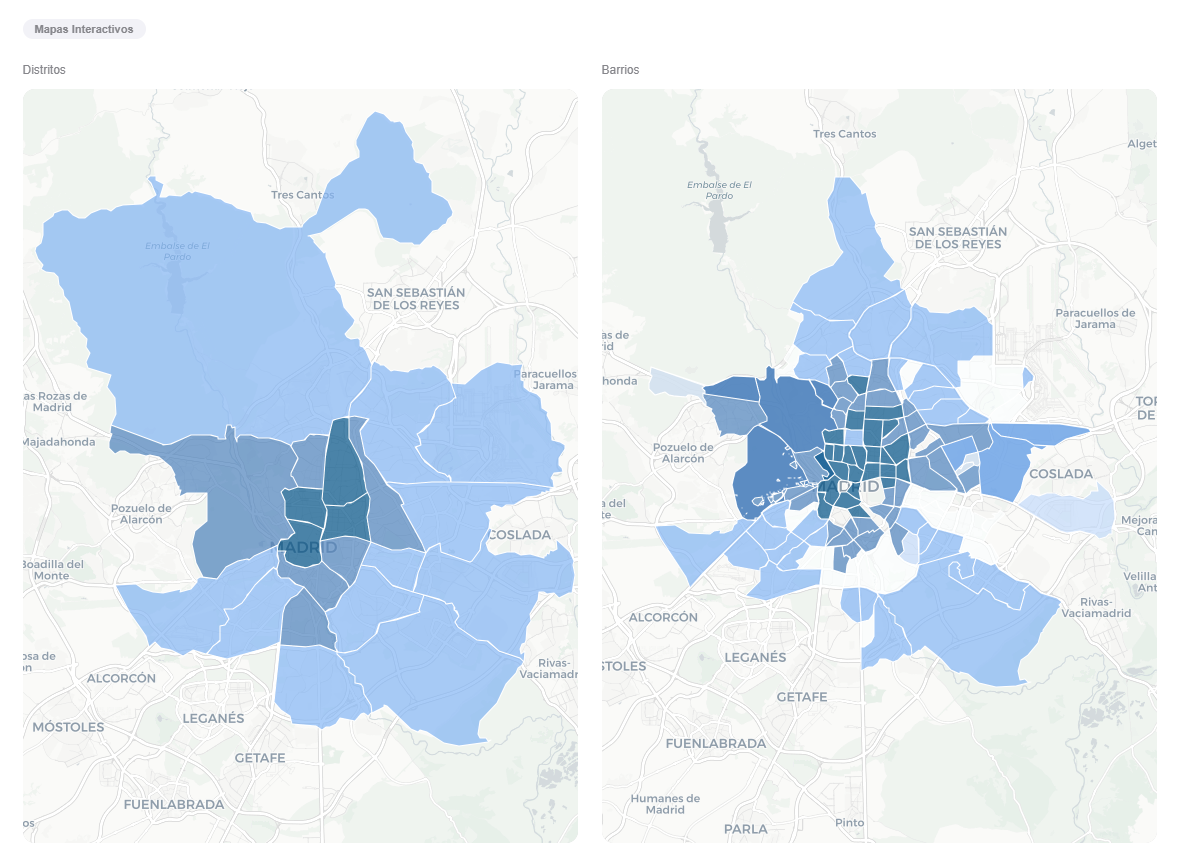
\includegraphics[width=0.65\textwidth]{img/mapa_interactivo.png}
        \caption{Mapa coroplético interactivo para la visualización cartográfica de precios.}
        \label{fig:mapa_interactivo}
    \end{figure}

    \item \textbf{Indicadores Clave de Negocio (KPIs):} Panel que expone en tiempo real cinco métricas esenciales del mercado local: precio medio unitario por metro cuadrado (\text{€/m\textsuperscript{2}}), ticket medio (precio total absoluto estimado de la transacción o mensualidad en la zona, proporcionando una referencia de coste total real frente al valor unitario), estado dinámico de tendencia del mercado (en crecimiento, estable o en reducción), variación intermensual frente al mes anterior (\%) y variación interanual frente al mismo mes del año previo (\%).
    \begin{figure}[H]
        \centering
        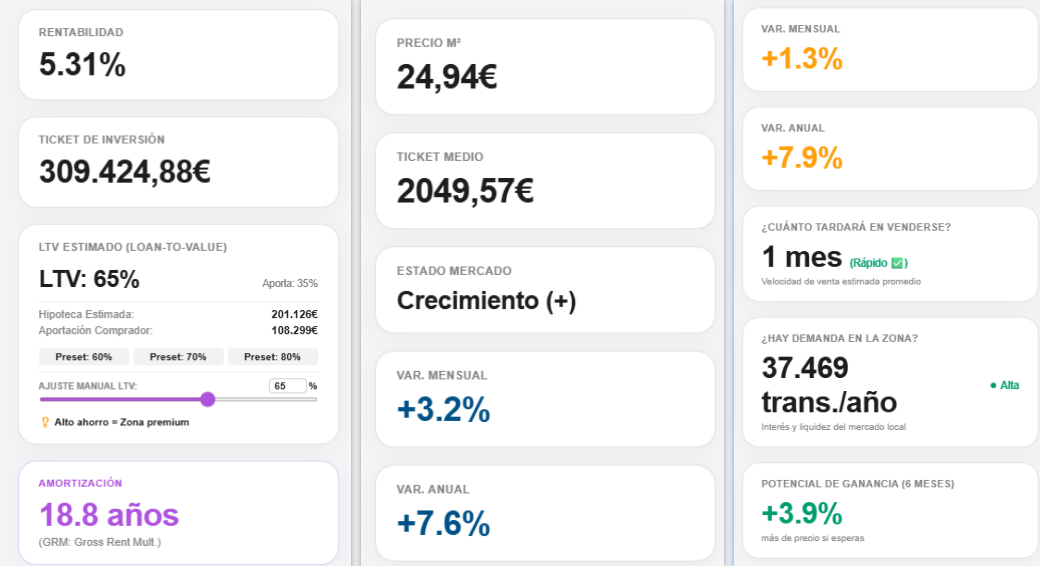
\includegraphics[width=0.65\textwidth]{img/algunos_indicadores_claves.png}
        \caption{Indicadores clave de negocio (KPIs) expuestos en tiempo real en el panel analítico.}
        \label{fig:indicadores_claves}
    \end{figure}
\end{itemize}

\section{Detalle de los Paneles de Control por Perfil de Usuario}
Aunque la interfaz mantiene una estructura y controles comunes, es inevitable y necesario que la lógica interna de los simuladores y la presentación de variables se desestructure por perfiles individuales. Integrar todos los perfiles en un único panel degradaría la usabilidad al mezclar KPIs y gráficos con objetivos dispares. A continuación, se detallan el modelado interactivo y los perfiles de usuario implementados.

\subsection{Modelado Financiero Interactivo basado en Datos Públicos (Enfoque Sin Asunciones)}
El acceso a la vivienda y la evaluación del mercado inmobiliario local suelen verse limitados en las herramientas de visualización tradicionales por la adopción de premisas arbitrarias y simplistas sobre la situación financiera de los usuarios. Para solucionar esta deficiencia metodológica, la plataforma \textit{Madrid Urban Intelligent} implementa una arquitectura modular de simulación financiera que separa de forma estricta los datos de carácter público de la información privada del ciudadano. Este enfoque metodológico, caracterizado como \textit{sin asunciones}, garantiza que la herramienta sirva como un motor de análisis neutral y objetivo que no presume a priori la solvencia, capacidad de ahorro o perfil de riesgo del usuario.

La estructura lógica de este modelado se divide en dos partes fundamentales (ver Figura~\ref{fig:comparativa_estructura}):
\begin{itemize}
    \item \textbf{Parte 1: Datos del Mercado (Público):} El sistema expone de forma transparente las variables objetivas de la zona (tales como el precio medio por metro cuadrado, el alquiler medio de mercado, la renta neta media por hogar del Instituto Nacional de Estadística (INE), y el volumen anual de transacciones registradas). A partir de estos datos, se calculan de manera directa métricas de referencia territorial como el multiplicador de alquiler bruto (GRM), la rentabilidad anual neta esperada (ROI) y la tasa de esfuerzo media del barrio.
    \item \textbf{Parte 2: Personalización (Opcional):} Se habilita un panel interactivo opcional donde el propio usuario introduce sus parámetros financieros personales (ingresos netos mensuales, ahorros disponibles o capital de inversión). El sistema recalcula en tiempo real las métricas de esfuerzo real, años de adquisición y viabilidad hipotecaria para su caso individual, sin necesidad de almacenar o transmitir información sensible.
\end{itemize}

\begin{figure}[H]
    \centering
    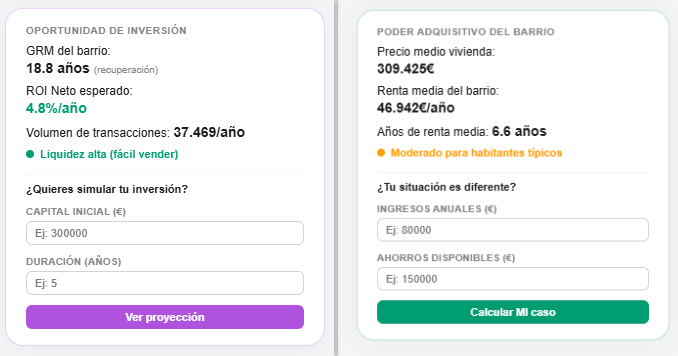
\includegraphics[width=0.65\textwidth]{img/introducir_datos_manuales.png}
    \caption{Panel interactivo de personalización financiera mediante introducción manual de datos del usuario.}
    \label{fig:comparativa_estructura}
\end{figure}


\subsection{Ventajas Metodológicas del Enfoque Sin Asunciones}
\label{subsec:ventajas_sin_asunciones}
Esta separación metodológica ofrece cuatro ventajas sustanciales: garantiza la \textbf{privacidad del ciudadano} al computar las simulaciones íntegramente en el cliente sin transmitir datos sensibles a servidores externos; asegura la \textbf{transparencia del dato base}, pues los valores del INE y el DataMart permanecen visibles e inalterados; proporciona \textbf{flexibilidad analítica} ante perfiles financieros diversos, incluyendo inversores patrimoniales, compradores extranjeros o jubilados con elevado capital acumulado; y refuerza la \textbf{credibilidad académica y técnica} al sustentar cada diagnóstico exclusivamente en los parámetros que el propio usuario introduce.


\subsection{Perfil Alquiler (Arrendatarios)}
El Perfil de Alquiler está concebido para optimizar la búsqueda de vivienda de arrendatarios (por ejemplo, estudiantes con recursos fijos o trabajadores en movilidad geográfica) y se organiza en torno a las siguientes funcionalidades clave:
\begin{itemize}
    \item \textbf{Módulo de Esfuerzo de Alquiler (Figura~\ref{fig:comparativa_alquiler}):} Muestra el coste de arrendamiento medio del barrio y la renta mensual estimada según el censo del INE, calculando la tasa de esfuerzo promedio. Al introducir sus ingresos netos mensuales, el simulador computa la tasa de esfuerzo real y clasifica la viabilidad en tres zonas de estrés financiero mediante una escala semafórica:
    \begin{itemize}
        \item \textit{Zona Verde (Tranquilo):} Esfuerzo inferior al 25\%.
        \item \textit{Zona Naranja (Justo):} Esfuerzo situado entre el 25\% y el 35\% (límite de seguridad recomendado en torno al 30\%).
        \item \textit{Zona Roja (Imposible):} Esfuerzo igual o superior al 35\%, indicando un riesgo de sobreendeudamiento severo. Si el esfuerzo calculado supera los umbrales de seguridad financieros, el sistema alerta de forma explícita al usuario sobre las limitaciones económicas de esa zona para su perfil financiero.
    \end{itemize}
    
    \item \textbf{Exploración de Viviendas Asequibles:} Integra un listado ordenado de las 10 zonas con mejor viabilidad financiera de la capital. Este módulo ayuda al usuario a identificar rápidamente distritos y barrios con precios de alquiler unitarios más bajos, destacando zonas periféricas altamente competitivas como Puente de Vallecas.
    
    \item \textbf{Evolución y Planificación Estacional:} Facilita el análisis mediante gráficos temporales cuándo bajan los precios en un distrito o barrio específico. Al identificar tramos estacionales económicos (por ejemplo, caídas recurrentes detectadas en enero y febrero o en junio y julio en ciertos distritos residenciales), el arrendatario puede planificar estratégicamente su mudanza para optimizar el alquiler mensual. De forma análoga, el propietario puede analizar los picos estacionales de rentabilidad para ofertar sus viviendas. Las trayectorias reflejan patrones diferenciados por zonas, tal como se aprecia en el análisis temporal del perfil de alquiler (Figura~\ref{fig:comparativa_alquiler}): Arganzuela muestra una tendencia alcista constante y lineal; Moncloa-Aravaca experimenta repuntes pronunciados a finales del verano e inicios de año vinculados a la movilidad universitaria; mientras que San Blas registra correcciones a la baja al cierre del año (septiembre a diciembre).
    
    \item \textbf{Comparador de Zonas Residenciales:} Facilita enfrentar directamente la dinámica de dos áreas de interés (por ejemplo, Distrito A vs. Distrito B). Mediante visualizaciones superpuestas en un único gráfico, se contrasta la evolución del precio/m², el ROI de alquiler y el esfuerzo requerido, contrastando ambas curvas frente a la media ponderada del municipio de Madrid (verificando de forma objetiva si zonas como Ciudad Lineal o Moratalaz operan por encima o por debajo del comportamiento general de la capital).
    
    \item \textbf{Proyecciones Predictivas Futuras:} En periodos donde el censo carece de valores reales o para horizontes futuros (2026), el panel expone las predicciones mensuales del modelo LightGBM. Se integra un indicador explícito que avisa de que se trata de un \textit{precio predicho}, lo que ayuda al ciudadano anticipar cambios de tendencia antes de la publicación de datos históricos oficiales.
\end{itemize}

\begin{figure}[H]
    \centering
    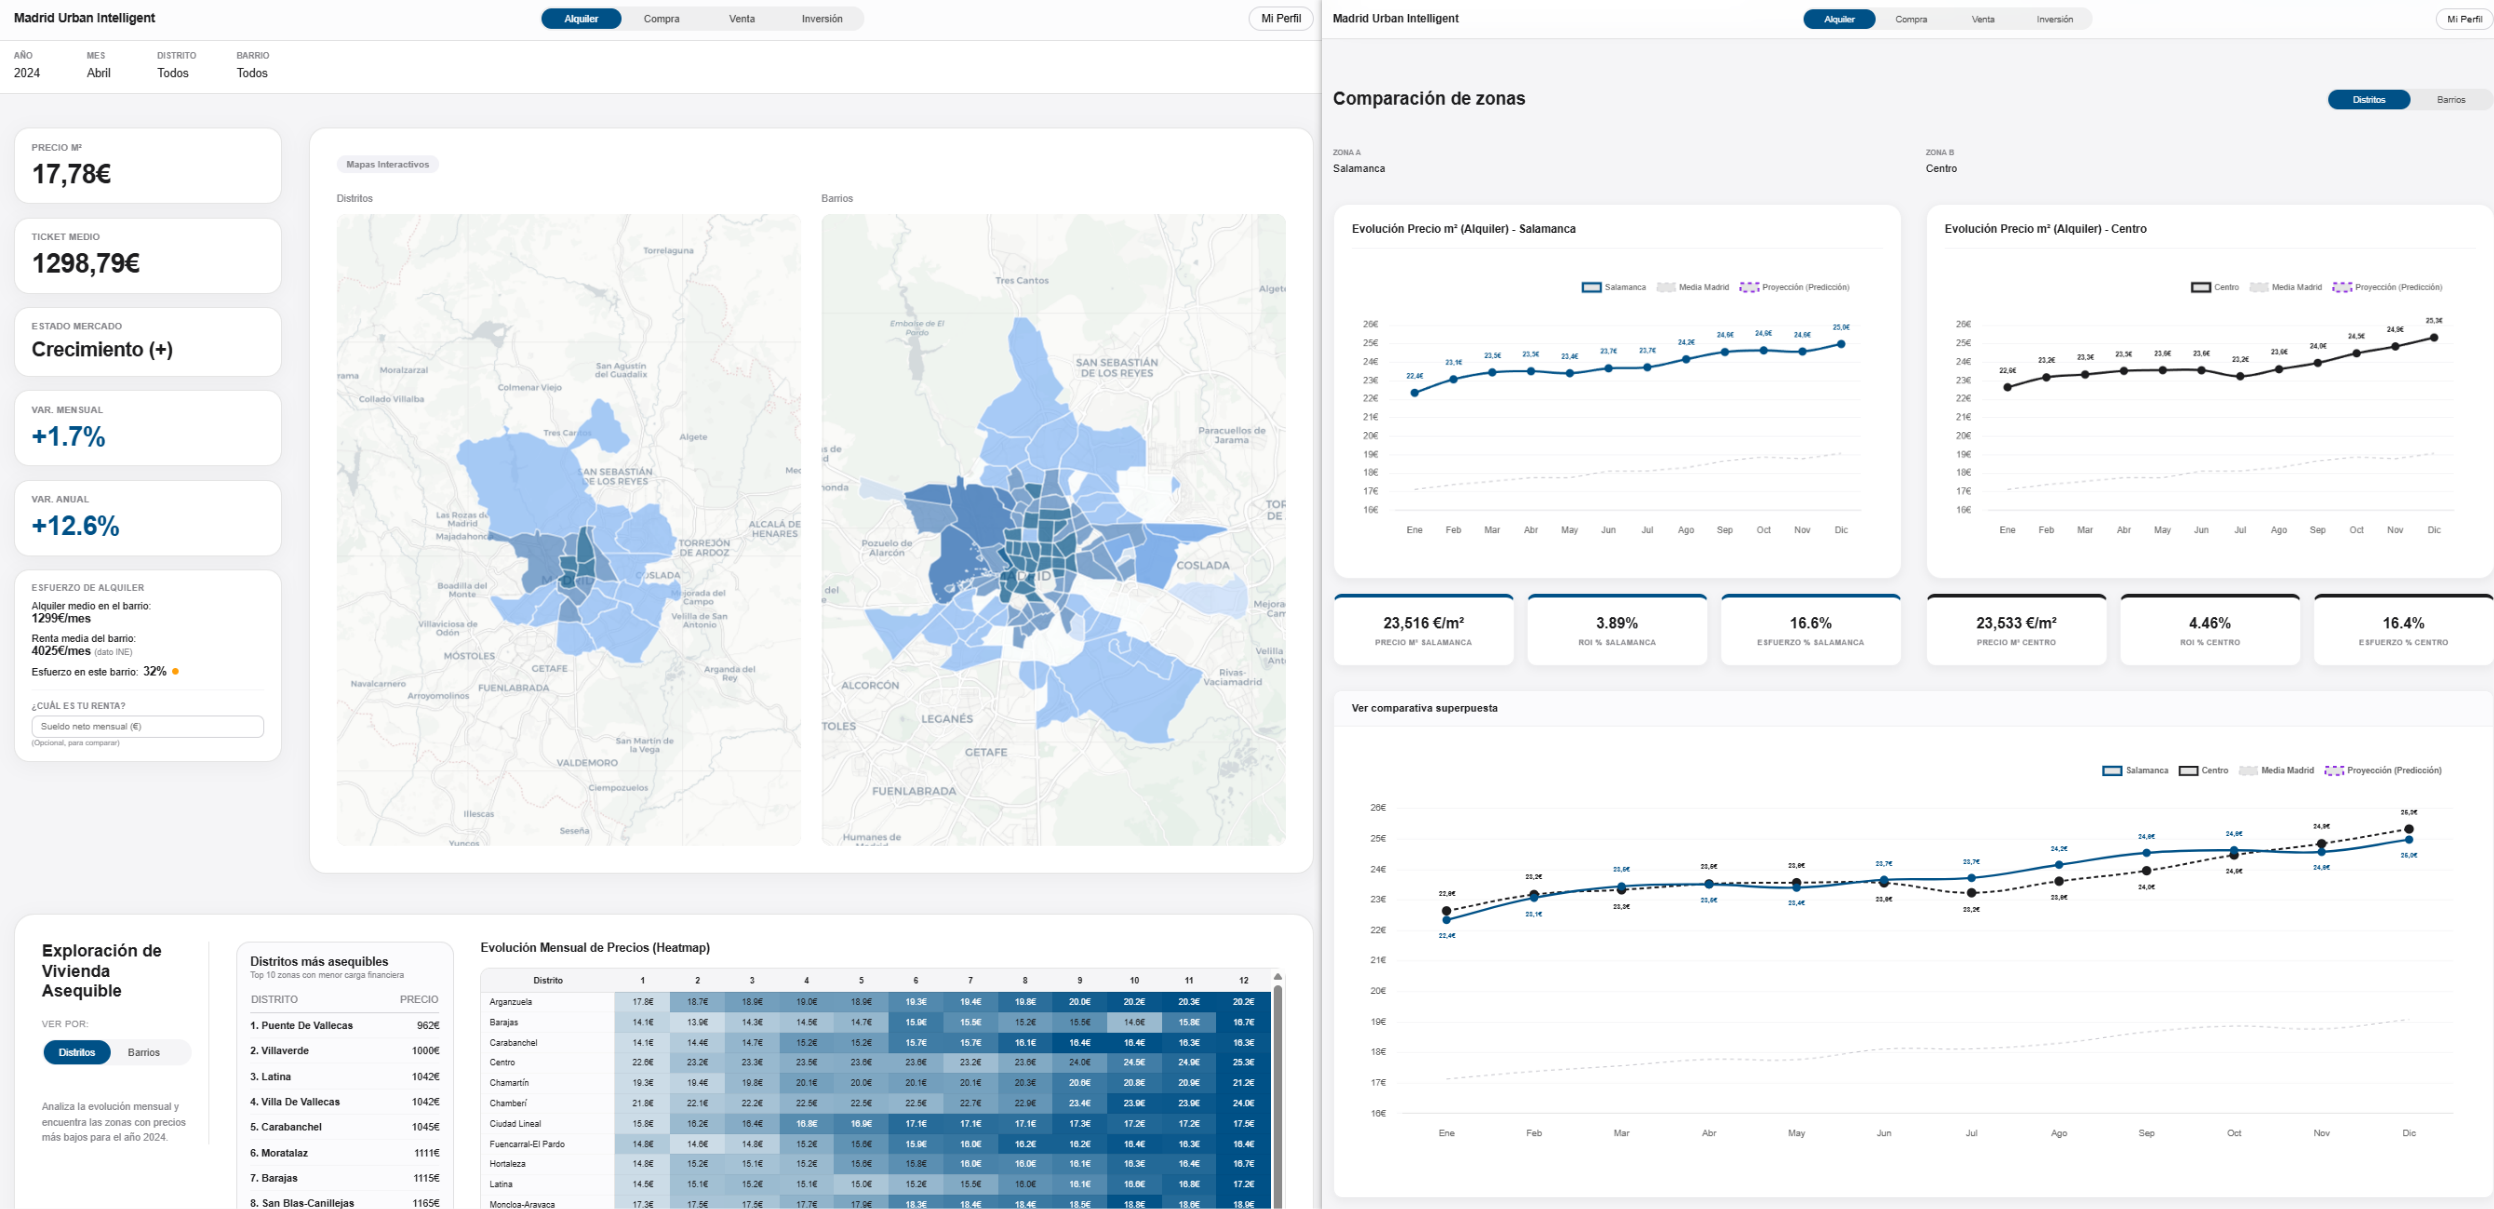
\includegraphics[width=0.95\textwidth]{img/alquiler.png}
    \caption{Interfaz del panel analítico correspondiente al Perfil Alquiler (Arrendatarios), mostrando los simuladores de esfuerzo financiero y la asequibilidad de las zonas.}
    \label{fig:comparativa_alquiler}
\end{figure}

\subsection{Perfil Compra (Compradores)}
El Perfil de Compra asiste a compradores de vivienda habitual en la evaluación de la viabilidad financiera de una compraventa de largo plazo. En términos de diseño de interfaz, este panel mantiene una consistencia estructural con el resto de la aplicación web; integra la cartografía dinámica mediante un mapa coroplético, un visor dinámico en formato de mapa de calor (\textit{heatmap}) para la evolución mensual de precios, un listado de las 10 zonas y barrios más asequibles de Madrid para la compra de activos, y los menús desplegables de distrito y barrio para el filtrado geográfico. Asimismo, hereda las funcionalidades de comparación multinivel, lo que facilita al usuario analizar la comparativa de variables lado a lado de dos zonas de forma individual o mediante un gráfico de curvas de evolución temporal superpuestas (ver Figura~\ref{fig:dashboard_compra}).

Sin embargo, a nivel de indicadores y simuladores, este panel introduce elementos específicos del segmento de adquisición:
\begin{itemize}
    \item \textbf{Indicadores Clave de Compra:} Muestra el precio medio unitario por metro cuadrado (\text{€/m\textsuperscript{2}}), el ticket medio de compra (que representa el precio promedio absoluto estimado para adquirir una vivienda en el barrio o distrito seleccionado), el estado dinámico del mercado (clasificándolo como estable, en crecimiento o en declive en base a la inercia local), y las variaciones mensuales e interanuales del precio de venta.
    \item \textbf{Simulador de Poder Adquisitivo y Viabilidad:} Relaciona en tiempo real variables fundamentales como el precio medio de la vivienda de la zona, la renta media por hogar registrada en el INE y el indicador de años de renta media necesarios para la adquisición (que mide el esfuerzo teórico en salarios íntegro necesarios para una familia local).
    \item \textbf{Personalización Financiera y Escenarios:} Facilita al usuario introducir manualmente sus ingresos anuales y ahorros disponibles. El sistema recalcula dinámicamente la viabilidad y, de manera adicional para perfiles con interés inversor, estima los años de alquiler mensual requeridos para amortizar la inversión inicial, identificando el umbral de rentabilidad de la adquisición.
    \item \textbf{Simulación de Hipoteca y Precios Predichos:} Realiza una simulación hipotecaria realista empleando los parámetros vigentes del Banco de España (tipo de interés, plazo y entrada aportada) y los gastos de compraventa de la Comunidad de Madrid, contrastando las cuotas mensuales frente a las tendencias futuras proyectadas por los modelos predictivos XGBoost.
\end{itemize}

\begin{figure}[H]
    \centering
    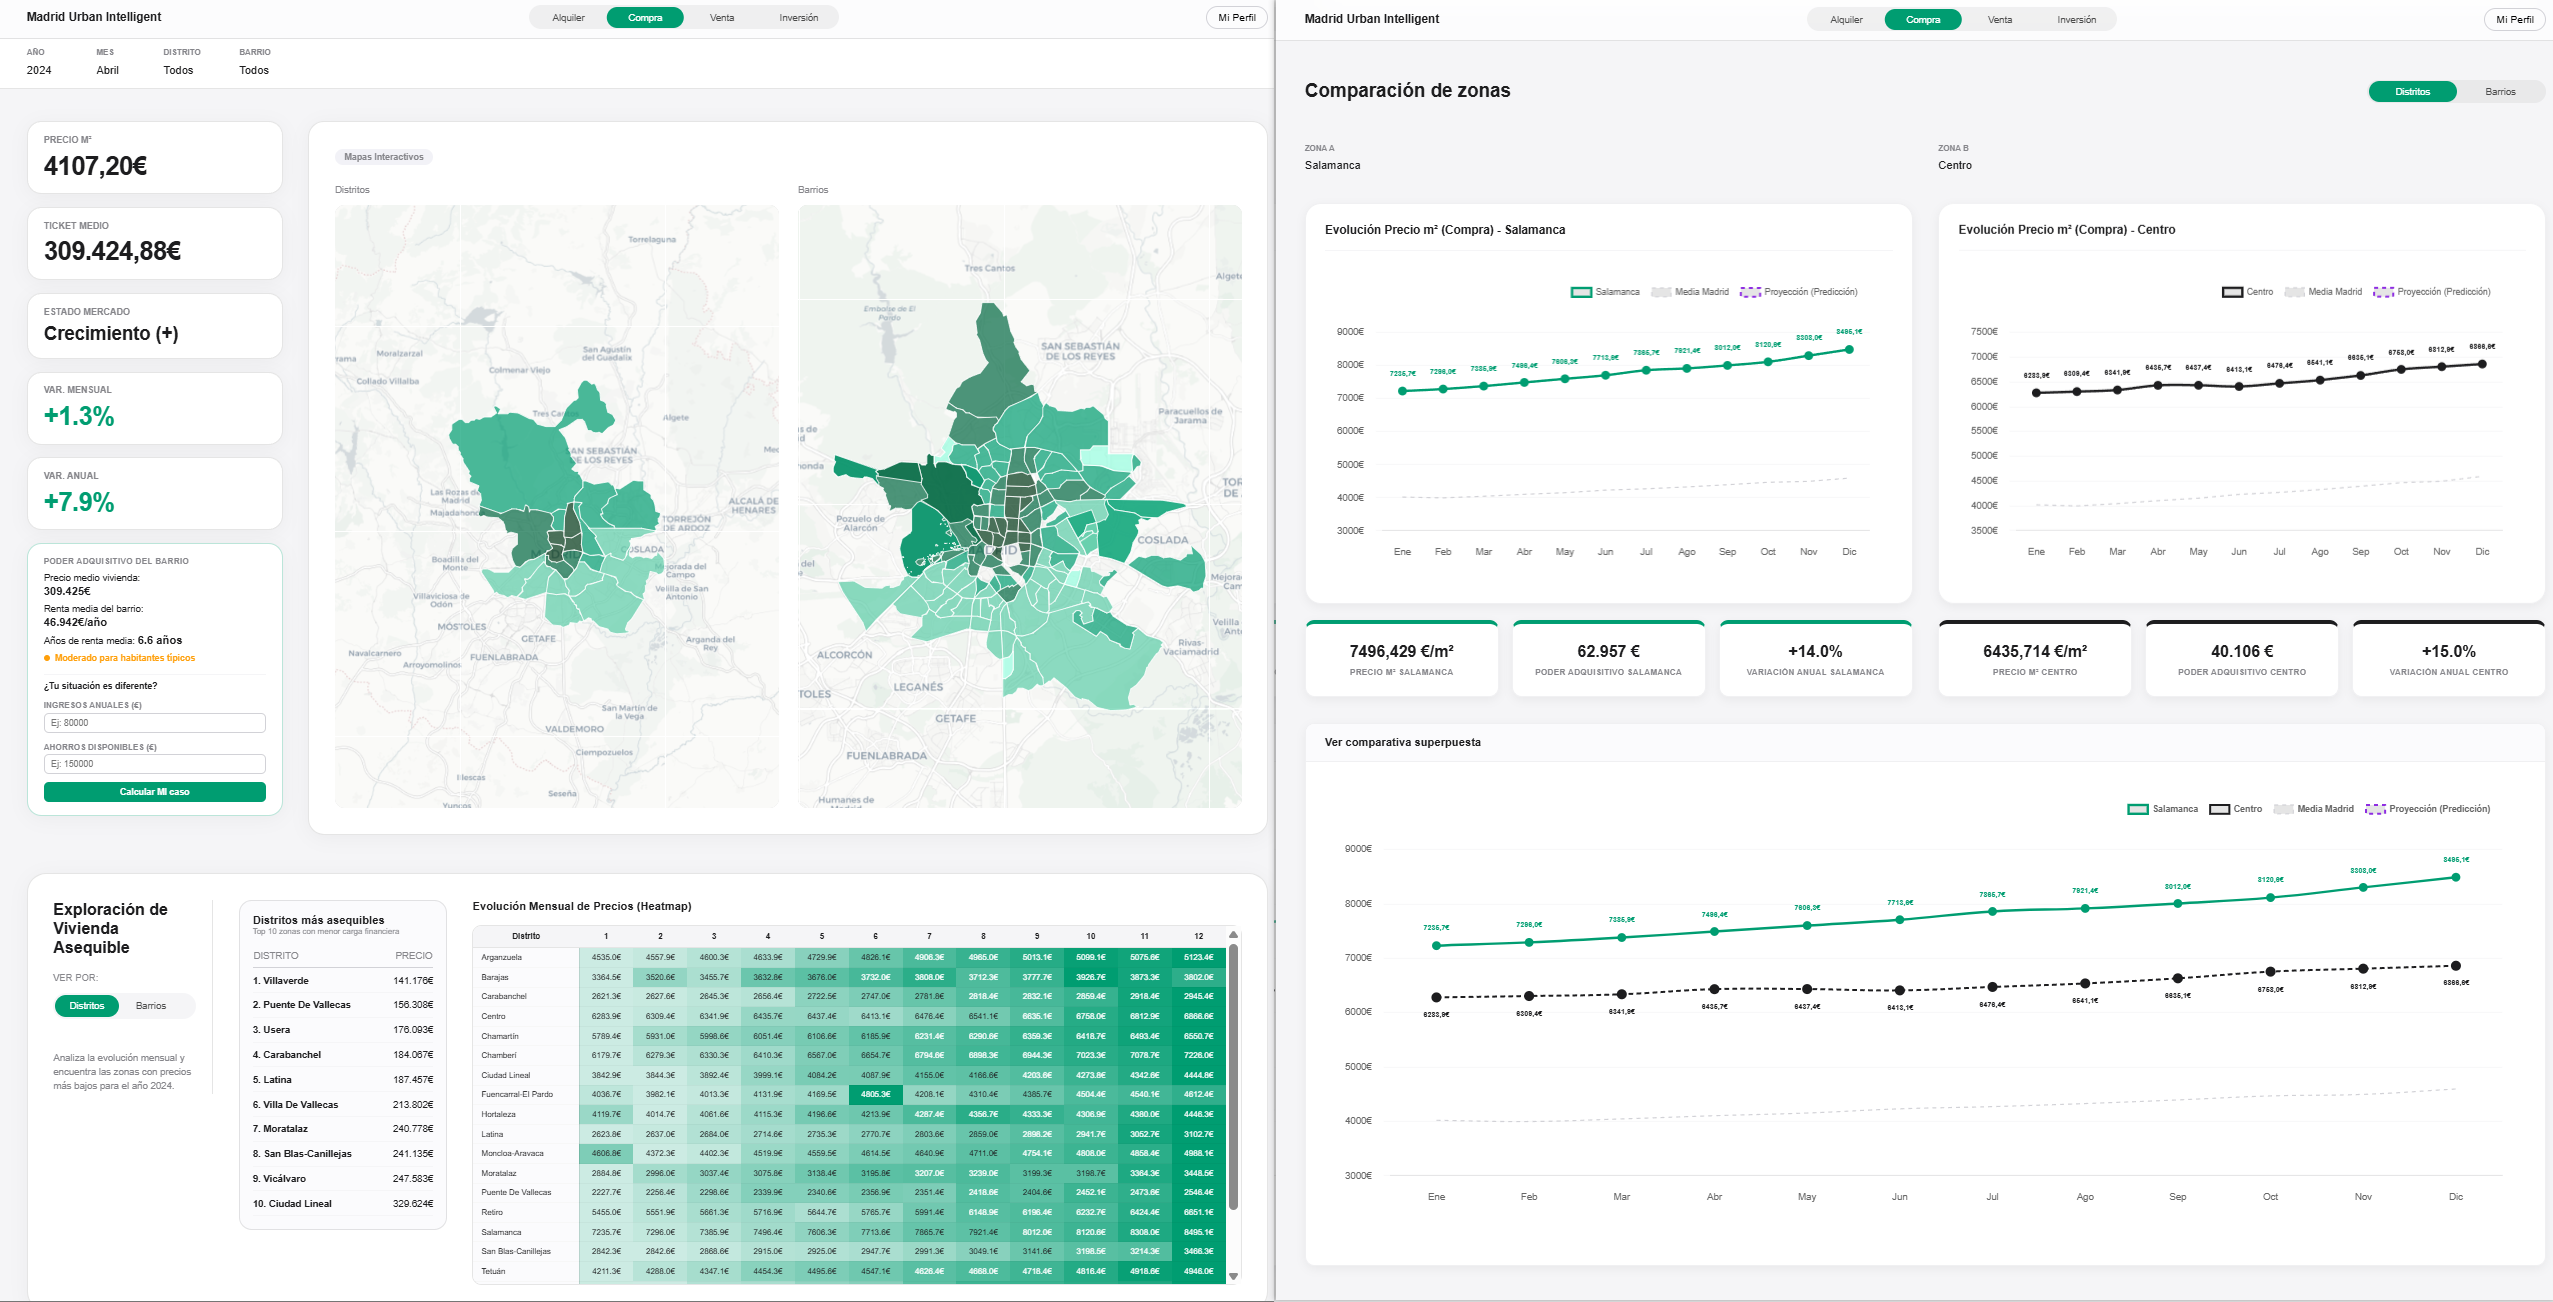
\includegraphics[width=0.95\textwidth]{img/compra.png}
    \caption{Interfaz del panel analítico correspondiente al Perfil Compra (Compradores), que incluye el simulador hipotecario y las proyecciones de asequibilidad.}
    \label{fig:dashboard_compra}
\end{figure}

\subsection{Perfil Venta (Propietarios)}
Diseñado para propietarios que desean valorar de forma independiente su patrimonio o estimar el rendimiento de la liquidación de sus activos residenciales. Este panel conserva la estructura general de visualización cartográfica, la evolución mensual del precio de venta, la lista de zonas con mayor valor de mercado, y la sección de comparativa de zonas (ver Figura~\ref{fig:dashboard_venta}). 

No obstante, en la vista del panel general y en la zona de comparación, se destacan indicadores críticos de volumen de operaciones y liquidez:
\begin{itemize}
    \item \textbf{Tasación Automatizada Local:} A través de un formulario sencillo en el que se introducen los metros cuadrados construidos y el barrio, el sistema realiza una consulta en tiempo real a los modelos predictivos XGBoost para devolver una valoración de mercado ajustada a las dinámicas del barrio.
    \item \textbf{Velocidad de Venta (Tiempo Medio en Mercado):} Muestra una estimación en meses del tiempo medio que tardaría en venderse un activo en la demarcación seleccionada (situada en una mediana histórica de 2,3 meses en el mercado activo de Madrid, calculada a partir del análisis de permanencia y rotación de anuncios consolidados en el DataMart para el periodo 2023--2025 (véase Sección~\ref{sec:enriquecimiento})). Este indicador facilita al propietario evaluar la agilidad del mercado local.
    \item \textbf{Demanda Activa y Liquidez Transaccional:} Mapea el volumen real de transacciones anuales acumuladas en la zona (promediando unas 406 transacciones anuales en el municipio durante el periodo de estudio 2023--2025, dato calculado a partir de las compraventas del Colegio de Registradores de España integradas en el DataMart) como indicador directo del volumen de transacciones y número de compradores activos en el mercado.
    \item \textbf{Potencial de Ganancia y Plusvalía Proyectada:} Muestra la plusvalía estimada de venta en los primeros 6 meses de tenencia del activo. Esta métrica computa el incremento patrimonial bruto proyectado basándose en las tasas de crecimiento intermensual estacionalmente ajustadas a nivel de barrio (los coeficientes dinámicos calculados mediante modelos autorregresivos en el pipeline de datos), haciendo posible prever el rendimiento a corto plazo de su activo.
    \item \textbf{Comparativa de Propiedades y Mercado:} Facilita la comparación de dos distritos o barrios, destacando en el comparador tres variables clave del vendedor: el precio unitario del metro cuadrado, la velocidad de venta media y la variación anual del precio de venta.
\end{itemize}

\begin{figure}[H]
    \centering
    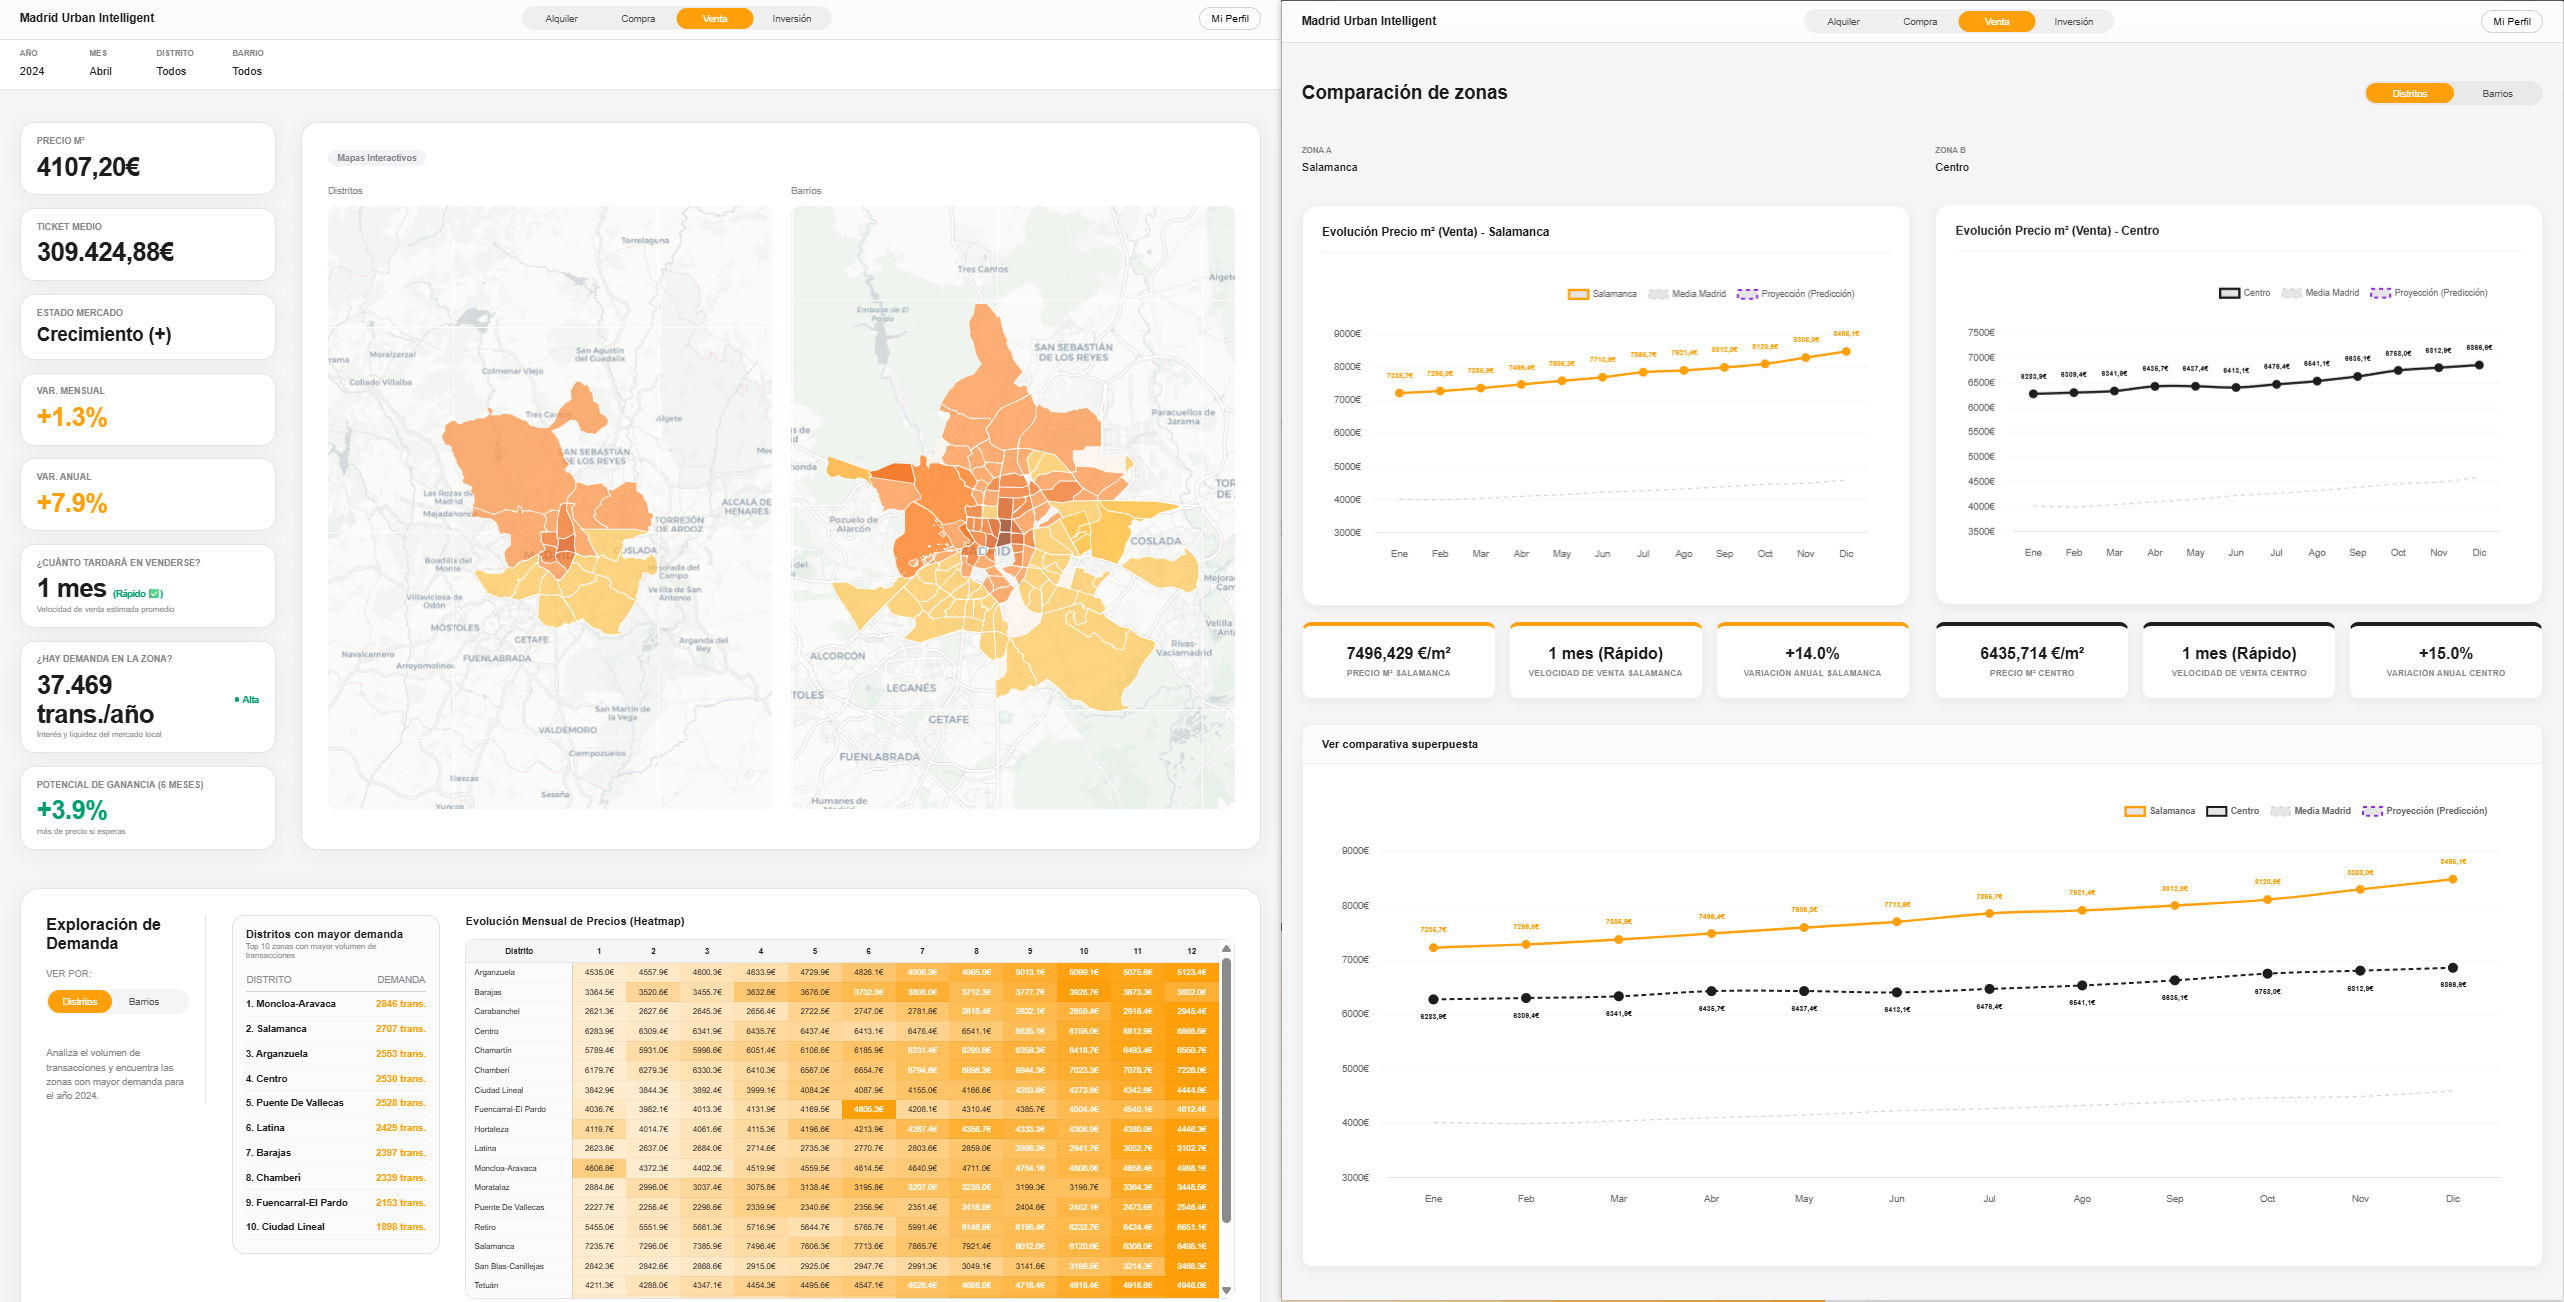
\includegraphics[width=0.95\textwidth]{img/venta.png}
    \caption{Interfaz del panel analítico correspondiente al Perfil Venta (Propietarios), con el módulo de tasación automatizada y estimaciones de velocidad de venta.}
    \label{fig:dashboard_venta}
\end{figure}

\subsection{Perfil Inversión (Inversores)}
Constituye el módulo analítico más complejo, orientado a inversores minoristas e institucionales para la colocación eficiente de capital en el mercado de suelo urbano residencial. El panel utiliza la estructura coroplética interactiva y temporal de la aplicación, pero la adapta para exponer métricas complejas de análisis técnico y viabilidad financiera (ver Figura~\ref{fig:dashboard_inversion}):
\begin{itemize}
    \item \textbf{LTV Estimado (\textit{Loan to Value}):} Calcula el porcentaje de financiación de la operación basándose en la hipoteca estimada necesaria y la aportación inicial de capital del comprador (fondos propios). El panel facilita ajustar dinámicamente esta relación para observar el apalancamiento financiero óptimo.
    \item \textbf{Gross Rent Multiplier (GRM) y Amortización:} Representa el multiplicador de alquiler bruto. Mapea la cantidad de años de alquiler bruto promedio necesarios para recuperar la inversión inicial en la vivienda de acuerdo con los precios y rentas de alquiler vigentes en la demarcación.
    \item \textbf{Métrica Yield y Retorno Neto (ROI):} Evalúa la rentabilidad bruta anual (\textit{Yield}) y el PER (años para amortizar la inversión mediante el arrendamiento neto) representados cartográficamente. Integra además un factor corrector del 90\% para deducir gastos de mantenimiento, comunidad e IBI, calculando el ROI neto de mercado.
    \item \textbf{Oportunidad de Inversión y Dinamismo:} Combina de forma analítica el GRM de la zona, el ROI neto estimado y el número de transacciones registradas durante el año como indicador de liquidez para la salida de la inversión.
    \item \textbf{Simulador de Capitalización Compuesta:} Facilita al inversor ingresar el capital inicial y la duración en años de la inversión. A partir de estas variables, proyecta una tabla detallada con la ganancia total absoluta y la ganancia anualizada media en euros, facilitando el análisis de la rentabilidad temporal de su capital.
\end{itemize}

\begin{figure}[H]
    \centering
    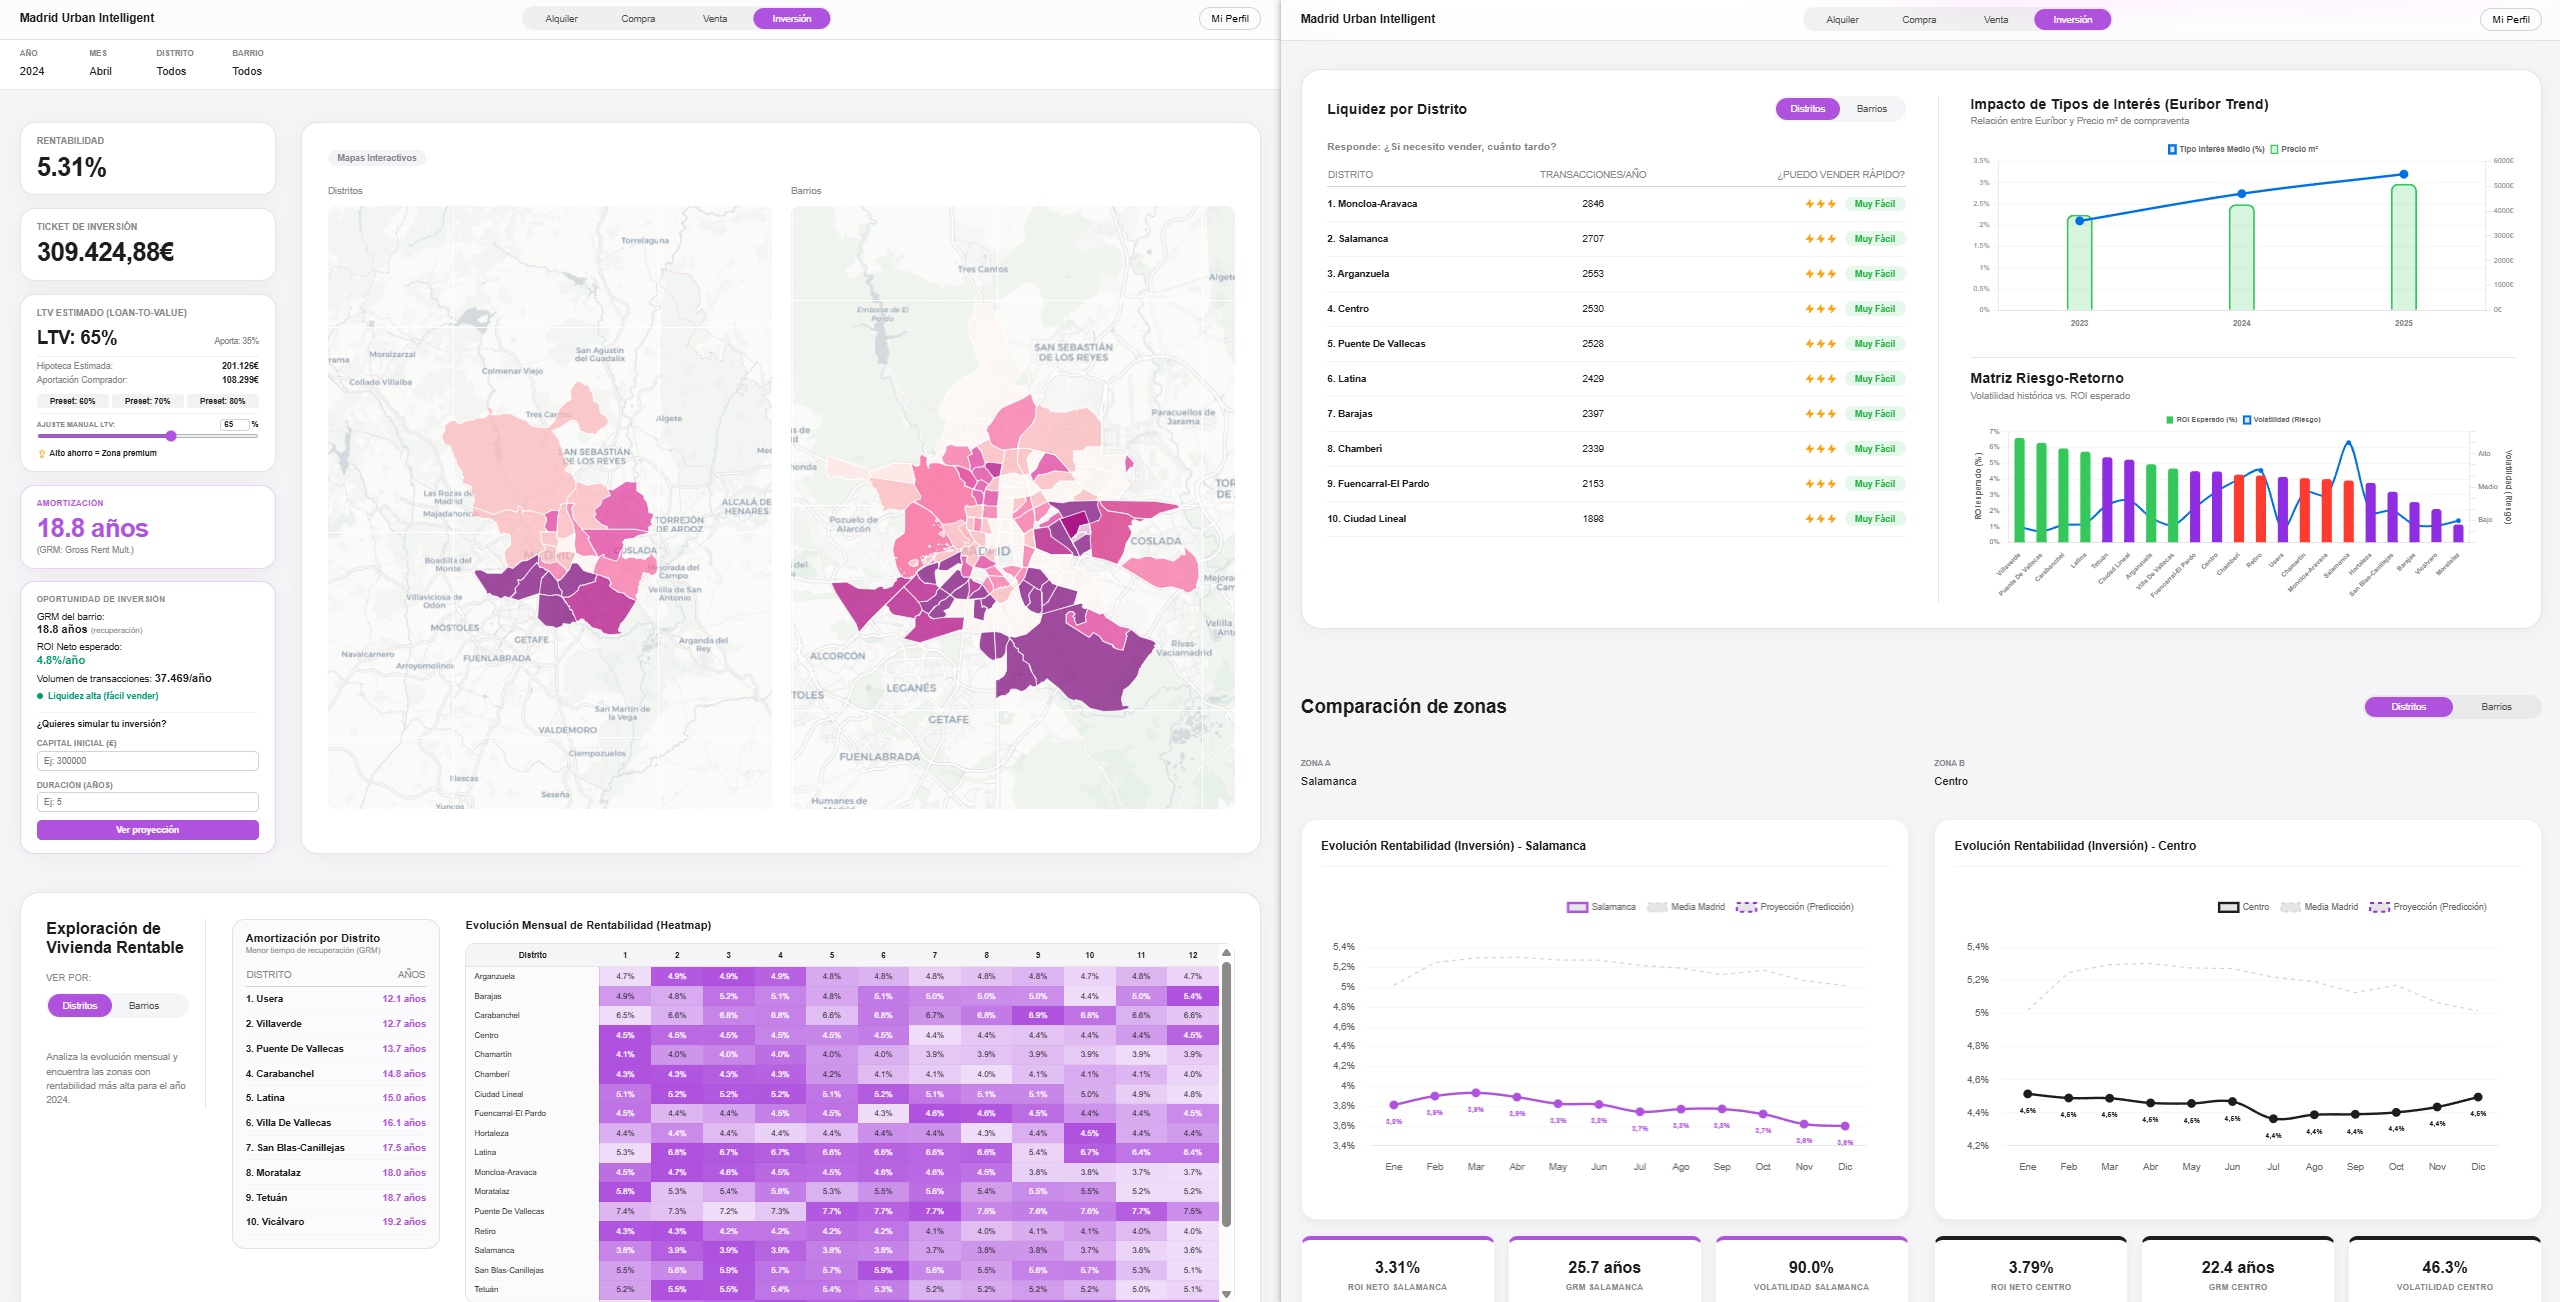
\includegraphics[width=0.95\textwidth]{img/inversion.png}
    \caption{Interfaz del panel analítico correspondiente al Perfil Inversión (Inversores), exponiendo los indicadores de rentabilidad bruta (Yield), PER y simulaciones de capitalización.}
    \label{fig:dashboard_inversion}
\end{figure}

\section{Visualizaciones Espaciales, Temporales e Interactividad}
La eficacia de la transferencia de conocimiento en la plataforma analítica se apoya en la interfaz de visualización geográfica y temporal, la cual ayuda a decodificar la complejidad de las dimensiones del DataMart. Para ello, se han desarrollado dos componentes visuales altamente interactivos y dinámicos: el mapa geoespacial y el visor de series temporales.

\subsection{Cartografía Geoespacial Interactiva (Choropleth Maps)}
La representación espacial se implementa mediante mapas coropléticos interactivos construidos sobre la librería geoespacial \textbf{Leaflet}. Estos mapas cargan de forma dinámica un objeto vectorial en formato GeoJSON que delimita geométricamente los 131 barrios que integran el municipio de Madrid. 

Las variables expuestas de forma interactiva en la cartografía al pasar el cursor (emergente del mapa coroplético) se adaptan dinámicamente según el perfil de usuario activo. Mientras que métricas complementarias como la renta neta media por hogar o las tasas de esfuerzo se visualizan por separado en las tarjetas de indicadores clave (KPIs) del panel, la ventana emergente sobre el mapa se limita estrictamente a los siguientes datos clave por demarcación geográfica:
\begin{itemize}
    \item \textbf{Perfil Alquiler (Arrendatarios):} Expone el precio medio del alquiler por metro cuadrado (\text{€/m\textsuperscript{2}}) y el precio de alquiler mensual promedio de la vivienda.
    \item \textbf{Perfil Compra (Compradores):} Muestra el precio medio de compra por metro cuadrado (\text{€/m\textsuperscript{2}}) y el precio de adquisición estimado de la vivienda.
    \item \textbf{Perfil Venta (Propietarios):} Presenta el precio medio de venta por metro cuadrado (\text{€/m\textsuperscript{2}}) y el precio promedio de mercado de la vivienda.
    \item \textbf{Perfil Inversión (Inversores):} Detalla el precio por metro cuadrado de compra (\text{€/m\textsuperscript{2}}), la rentabilidad bruta esperada (\textit{Yield}) y el alquiler estimado de la vivienda.
\end{itemize}

El cálculo de los gradientes de color y las tonalidades de los mapas coropléticos constituye un aspecto metodológico clave. En lugar de aplicar una única escala de color tricolor general o rangos absolutos y estáticos, la plataforma asocia una familia cromática exclusiva y específica a cada uno de los cuatro perfiles de usuario. Dentro de cada perfil, la escala de visualización no emplea una interpolación divergente (verde--amarillo--rojo), sino que utiliza la intensidad del tono (tonalidad clara, media, oscura o fuerte) basada en rangos dinámicos calculados mediante la distribución en percentiles (generalmente en tres o cuatro rangos de valor):
\begin{itemize}
    \item \textbf{Perfil Alquiler (Arrendatarios):} Se representa íntegramente en \textbf{tonos azules}, donde un azul claro denota precios más asequibles o económicos, un azul de intensidad media indica valores de renta intermedios y un azul oscuro e intenso destaca las zonas con los precios de alquiler más elevados por metro cuadrado.
    \item \textbf{Perfil Compra (Compradores):} Utiliza una escala de \textbf{tonos verdes}, donde los verdes suaves o claros representan precios de venta unitarios y ratios de esfuerzo bajos (más asequibles), y los verdes oscuros y de gran fortaleza denotan las áreas con mayor coste de adquisición y esfuerzo financiero severo.
    \item \textbf{Perfil Venta (Propietarios):} Se decanta por una gama de \textbf{tonos naranjas}, donde las tonalidades de color naranja claro y débil muestran los precios de venta unitarios más reducidos de la serie y los naranjas intensos y muy fuertes identifican las áreas con valoraciones de mercado más premium y elevadas plusvalías.
    \item \textbf{Perfil Inversión (Inversores):} Emplea una paleta de \textbf{tonos fucsia, rosa y morado}, en la cual los rosas suaves representan rentabilidades brutas bajas y los morados oscuros y fucsias intensos destacan las zonas con rendimientos brutos anuales más óptimos y elevados retornos.
\end{itemize}
Esta coherencia visual se extiende al mapa de calor; de este modo, ambos visores comparten la misma familia cromática para cada perfil respectivo.

\subsection{Análisis Temporal Comparativo (Chart.js)}
\label{subsec:analisis_temporal_chartjs}
Para complementar el análisis geográfico del mes en curso, la plataforma implementa en todos los perfiles de usuario (Alquiler, Compra, Venta e Inversión) un módulo de análisis temporal interactivo desarrollado con la librería \textbf{Chart.js}. Este componente resuelve una de las barreras de decisión habituales en el ciudadano (la indecisión o dilema entre dos alternativas) al permitir la selección y comparación directa y simultánea de dos zonas geográficas (Zona A y Zona B), configurables individualmente tanto a nivel de distrito como de barrio.

El gráfico representa la fluctuación mensual del indicador crítico de cada perfil (precios medios del metro cuadrado para Alquiler, Compra y Venta, y tasa de rentabilidad bruta anual para el Perfil Inversión), con un periodo continuo de cuatro años estructurado en dos tramos diferenciados visualmente:
\begin{itemize}
    \item \textbf{Tramo Histórico (Enero 2023 -- Marzo 2026):} Representa los valores históricos reales y consolidados basados en datos abiertos recuperados por el pipeline ETL. Para indicar que se trata de observaciones reales definitivas, el visor los representa mediante \textbf{líneas continuas}.
    \item \textbf{Tramo Predictivo (Abril 2026 -- Diciembre 2027):} Proyecta las predicciones mensuales calculadas por los algoritmos XGBoost (en compra y venta) y LightGBM (en alquiler). Para diferenciar claramente este periodo de estimación futura, el visor dibuja las curvas mediante \textbf{líneas punteadas}.
\end{itemize}

El visor Chart.js superpone tres curvas diferenciadas de forma simultánea, lo que permite realizar un análisis de contraste inmediato frente a la referencia municipal:
\begin{enumerate}
    \item \textbf{Curva de la Zona A (Barrio/Distrito A):} Muestra la evolución temporal y la estacionalidad del primer sector seleccionado, facilitando la identificación de tendencias locales y volatilidad.
    \item \textbf{Curva de la Zona B (Barrio/Distrito B):} Muestra la evolución paralela del segundo sector, lo que facilita al usuario evaluar de un vistazo cuál de las dos opciones ofrece mayor rentabilidad o precios más competitivos.
    \item \textbf{Curva de la Media de Madrid (Municipio - Capital):} Representa el promedio ponderado de toda la ciudad de Madrid. Esta curva actúa como línea de referencia de control para determinar de inmediato si los sectores comparados se comportan por encima o por debajo de la inercia global de la capital (lo que facilita contrastar de manera directa cómo un barrio en el distrito de \textit{Salamanca} evoluciona de forma sistemática por encima de la media municipal, mientras que un barrio en el distrito de \textit{Latina} se sitúa consistentemente por debajo).
\end{enumerate}

En síntesis, la interfaz modular y las visualizaciones interactivas de \textit{Madrid Urban Intelligent} trasladan el conocimiento analítico del DataMart predictivo al usuario final. Al estructurar la información por perfiles y facilitar comparativas espaciales y temporales dinámicas, la plataforma mitiga de manera efectiva la asimetría informativa característica del mercado inmobiliario. No obstante, para aquellos usuarios sin competencias técnicas en el manejo de interfaces visuales, se ha desarrollado un canal alternativo de consulta basado en el lenguaje natural, cuyo diseño y arquitectura conversacional a través de Modelos de Lenguaje de Gran Tamaño (LLMs) se expone en detalle en el Capítulo~\ref{chap:conversational_bot}.


% --- Capítulo 8: Asistente Conversacional Inteligente con LLM ---
\chapter{Asistente Conversacional Inteligente con LLM}
\label{chap:conversational_bot}
A pesar de la facilidad de uso de los cuadros de mando interactivos y las visualizaciones avanzadas descritas en el Capítulo~\ref{chap:web_frontend}, la presencia de bases de datos relacionales estructuradas sigue imponiendo una barrera técnica insalvable para el ciudadano medio, quien carece de conocimientos en lenguajes de consulta formal como SQL. Para facilitar el acceso general a la información y eliminar cualquier barrera de entrada, la plataforma \textit{Madrid Urban Intelligent} incorpora un asistente conversacional inteligente (chatbot) denominado \textbf{Ambi}. Esta herramienta permite a cualquier persona interrogar al sistema mediante lenguaje natural y recibir respuestas analíticas inmediatas acompañadas de resúmenes textuales de alta calidad.

\section{Arquitectura del Motor Conversacional (FastAPI + LLM)}
El asistente Ambi se estructura bajo una arquitectura de microservicios desacoplada. El frontend reactivo se conecta en tiempo real con un servicio web asíncrono implementado en el backend de FastAPI. Este backend expone un endpoint REST bajo la ruta \texttt{/api/chat} que recibe el historial de conversación y la consulta del usuario.

El motor conversacional de Ambi se ejecuta bajo un diseño local y privado para garantizar la soberanía de los datos y la total privacidad de la información del ciudadano, evitando los costes por llamada y las limitaciones de tokens asociadas a las APIs comerciales en la nube, aspectos determinantes durante el desarrollo y la evaluación del asistente. Para asegurar un procesamiento de bajo coste e independiente de la conectividad externa, el sistema ejecuta de forma nativa un modelo personalizado denominado \texttt{gemma4:e4b} (alias local asignado en el \textit{Modelfile} de Ollama, derivado del modelo base de código abierto \textbf{Gemma 2 (2B)} de Google (Gemma Team, Google, 2024)). Este modelo ha sido creado localmente mediante un archivo de configuración \textit{Modelfile} de Ollama a partir del modelo base de código abierto \textbf{Gemma 2 (2B)} de Google (de 2.6 mil millones de parámetros), al cual se le ha inyectado un prompt de sistema específico para el rol de consultor inmobiliario de Madrid y se ha ajustado su temperatura de inferencia a $0.3$ para maximizar la precisión analítica y evitar respuestas creativas; el modelo se ejecuta a través del motor de inferencia de alto rendimiento de \textbf{Ollama}.

A nivel de recuperación de información, el sistema implementa una \textbf{Arquitectura RAG Híbrida} que combina datos estructurados y no estructurados:
\begin{itemize}
    \item \textbf{Contexto Estructurado (KPIs):} El backend analiza la consulta para extraer variables geográficas (distrito o barrio) y temporales (año). Posteriormente, realiza una consulta directa a la base de datos relacional mediante funciones en Python para recuperar métricas precisas de precios, variaciones y esfuerzo. Estos datos exactos se inyectan directamente en el prompt del sistema, eliminando cualquier riesgo de alucinación numérica por parte del LLM.
    \item \textbf{Contexto No Estructurado (RAG Vectorial):} De manera paralela, el sistema utiliza un motor de búsqueda por similitud sobre una base de datos vectorial para recuperar información cualitativa del entorno (infraestructuras, colegios, centros de salud y transportes en un radio de 1 km).
\end{itemize}

El flujo conversacional completo consta de varias etapas clave que garantizan una experiencia fluida desde la consulta inicial del ciudadano hasta la respuesta final en la interfaz web, tal como se esquematiza en la Figura~\ref{fig:conversational_flow}.

\begin{figure}[H]
\centering
\shorthandoff{<>}
\begin{tikzpicture}[
    node distance=1.5cm,
    block/.style={rectangle, draw, fill=blue!10, text width=3.8cm, align=center, rounded corners, minimum height=1cm, font=\small},
    line/.style={draw, -stealth, thick}
]
    % Nodes
    \node (user) [block, fill=green!15] {\textbf{Usuario} \\ (Pregunta en lenguaje natural)};
    \node (backend) [block, below=of user] {\textbf{FastAPI Backend} \\ (Extracción de Entidades y KPIs)};
    \node (rag) [block, below left=1.2cm and 1.2cm of backend] {\textbf{Motor RAG Vectorial} \\ (ChromaDB + Embeddings)};
    \node (sqlite) [block, below right=1.2cm and 1.2cm of backend, fill=orange!15] {\textbf{DataMart SQLite} \\ (KPIs Estructurados)};
    \node (llm) [block, below=2.8cm of backend] {\textbf{Generador LLM Local} \\ (Ollama: gemma4:e4b)};
    \node (user_resp) [block, below=of llm] {\textbf{Interfaz Web} \\ (Respuesta Conversacional)};
    
    % Paths
    \path [line] (user) -- (backend);
    \path [line] (backend) -- (rag);
    \path [line] (backend) -- (sqlite);
    \path [line] (rag) -- (llm);
    \path [line] (sqlite) -- (llm);
    \path [line] (llm) -- (user_resp);
\end{tikzpicture}
\shorthandon{<>}
\caption{Flujo arquitectónico del asistente conversacional Ambi en la plataforma Madrid Urban Intelligent.}
\label{fig:conversational_flow}
\end{figure}

\section{Construcción del Pipeline de Ingesta y Vectorización (ChromaDB)}
Para alimentar el contexto no estructurado del asistente Ambi, se implementa un pipeline de ingesta automatizado (\texttt{ingest.py}) que transforma los registros de la base de datos relacional en documentos vectoriales. El proceso consta de las siguientes fases:
\begin{enumerate}
    \item \textbf{Recuperación y Síntesis:} Se extraen los últimos registros consolidados de cada barrio combinando las variables del mercado de venta, alquiler e infraestructuras locales. A partir de estos registros, se genera un párrafo descriptivo en lenguaje natural para cada uno de los 131 barrios de Madrid.
    \item \textbf{Generación de Embeddings:} Empleando el modelo multilingüe de HuggingFace \texttt{sentence-transformers/paraphrase-multilingual-MiniLM-L12-v2}, se codifican los textos generados en vectores densos de características semánticas.
    \item \textbf{Almacenamiento Vectorial:} Los vectores y sus metadatos asociados (barrio y distrito) se indexan en un almacén de vectores \textbf{ChromaDB} persistido localmente, lo que facilita búsquedas de similitud semántica con latencias del orden de milisegundos.
\end{enumerate}

\section{Flujo de Ejecución y Síntesis Conversacional}
Una vez construido el pipeline, el backend de FastAPI gestiona la interacción conversacional con Ambi mediante un flujo en cuatro pasos:
\begin{enumerate}
    \item \textbf{Extracción de Entidades y Contexto:} Al recibir el mensaje del usuario (por ejemplo: \textit{«¿Qué tal es la rentabilidad y el transporte en el barrio de Sol en 2026?»}), el backend limpia el texto y extrae las variables clave (barrio: Sol, año: 2026, operación: inversión).
    \item \textbf{Recuperación Híbrida:}
    \begin{itemize}
        \item Se consultan las tablas del DataMart relacional SQLite para obtener el precio medio, variación y rentabilidad del año solicitado.
        \item Se realiza una búsqueda por similitud en la base de datos ChromaDB utilizando el texto de la consulta del usuario para recuperar los documentos relacionados con las infraestructuras de transporte y servicios locales.
    \end{itemize}
    \item \textbf{Inyección de Contexto y Prompting:} Se fusiona el contexto de KPIs estructurados con los textos cualitativos recuperados de ChromaDB. Este bloque combinado se inyecta en el prompt de sistema (\textit{system prompt}) para guiar al modelo personalizado \texttt{gemma4:e4b} en Ollama en la redacción de la respuesta final.
    \item \textbf{Síntesis Conversacional y Memoria:} El LLM sintetiza la información y redacta una respuesta coherente y estructurada. El backend almacena el intercambio en un búfer de memoria conversacional con ventana deslizante (\textit{ConversationBufferWindowMemory}, con $k=5$ turnos) para mantener la coherencia del hilo de la conversación, devolviendo la respuesta al frontend React.
\end{enumerate}

\section{Evaluación Empírica del Motor Conversacional (Ambi)}
A diferencia de los cuadros de mando tradicionales, un asistente conversacional RAG (Retrieval-Augmented Generation) requiere una validación cualitativa y cuantitativa específica para medir la precisión en la recuperación del contexto y la veracidad de la síntesis final del LLM. Para evaluar el rendimiento de Ambi de forma empírica en un entorno local y controlado, se diseñó un banco de pruebas compuesto por 12 preguntas de validación realistas sobre el mercado inmobiliario de Madrid. 

Estas consultas cubren diversas tipologías de preguntas (precios de venta, alquiler, rentabilidad, infraestructuras y consultas fuera de dominio) y niveles de granularidad (distrito, barrio o genérica). La evaluación mide de forma manual tres indicadores fundamentales:
\begin{itemize}
    \item \textbf{Recuperación de Contexto (DataMart/Chroma):} Determina si el backend fue capaz de extraer las entidades correctas y recuperar los KPIs exactos del DataMart SQLite y los documentos de ChromaDB. Se califica como Correcta (C) o Incorrecta (I).
    \item \textbf{Precisión de la Respuesta del LLM:} Califica el texto final redactado por \texttt{gemma4:e4b} en tres categorías: Correcta (C) cuando responde de forma veraz y sin alucinaciones numéricas; Incompleta (Inc) si el contexto se recuperó pero la respuesta carece de algún detalle; o Errónea (E) en caso de alucinación semántica o matemática.
    \item \textbf{Latencia (segundos):} Registra el tiempo de respuesta total desde el envío de la consulta hasta la generación completa de la respuesta local (ejecutado sobre un hardware de pruebas con CPU Intel i7 y GPU RTX 3060 Laptop con 6 GB de VRAM empleando la cuantización por defecto del modelo de 4 bits en Ollama).
\end{itemize}

La Tabla~\ref{tab:evaluacion_ambi} expone el comportamiento detallado del asistente frente a este banco de pruebas.

\begin{table}[H]
\centering
\resizebox{1\linewidth}{!}{
\begin{tabular}{|c|p{7.5cm}|c|c|c|c|}
\hline
\textbf{ID} & \textbf{Pregunta del Usuario (Consulta Input)} & \textbf{Ámbito} & \textbf{Recuperación} & \textbf{Eval. LLM} & \textbf{Latencia (s)} \\ \hline
1 & «Precio del alquiler medio en Aluche en 2026» & Barrio & Correcta (C) & Correcta (C) & 1,22 \\ \hline
2 & «¿Cuál es el precio medio de venta en Retiro?» & Distrito & Correcta (C) & Correcta (C) & 0,95 \\ \hline
3 & «Barrios con mejor rentabilidad en Salamanca para invertir» & Híbrido & Correcta (C) & Correcta (C) & 1,58 \\ \hline
4 & «¿Cómo es el transporte público y metro en Sol?» & Vectorial & Correcta (C) & Correcta (C) & 1,15 \\ \hline
5 & «Rentabilidad bruta del alquiler en Barajas en 2026» & Barrio & Correcta (C) & Correcta (C) & 1,30 \\ \hline
6 & «Parques, colegios y zonas verdes en Chamberí» & Vectorial & Correcta (C) & Correcta (C) & 1,42 \\ \hline
7 & «¿Cuál es la renta media neta por hogar en Vallecas?» & Barrio & Correcta (C) & Correcta (C) & 1,02 \\ \hline
8 & «Precios de venta de pisos en Salamanaca» & Corrección & Correcta (C)* & Correcta (C) & 1,65 \\ \hline
9 & «¿Cuál es el barrio más barato de Madrid para alquilar?» & Genérica & Correcta (C) & Correcta (C) & 1,84 \\ \hline
10 & «Comparación de rentabilidad entre Tetuán y Usera en 2026» & Comparación & Correcta (C) & Correcta (C) & 2,12 \\ \hline
11 & «¿Qué línea de metro pasa por el barrio de Goya?» & Vectorial & Correcta (C) & Correcta (C) & 1,28 \\ \hline
12 & «¿Cuáles son los precios de venta de pisos en París?» & Fuera de Dominio & N/A (Filtro) & Correcta (C)** & 0,78 \\ \hline
\end{tabular}
}
\caption{Resultados del banco de pruebas empírico del asistente conversacional Ambi.}
\label{tab:evaluacion_ambi}
\end{table}

\begin{spacing}{1}
\small
\noindent \textbf{Notas sobre la tabla:} \\
(*) La consulta contenía un error ortográfico intencional («Salamanaca»). El algoritmo de Levenshtein en el backend corrigió el término a «Salamanca», lo que hizo posible la recuperación correcta de los KPIs. \\
(**) Ante consultas fuera del ámbito geográfico (Madrid), el modelo gemma4:e4b rechaza educadamente responder e indica sus límites temáticos y geográficos.
\end{spacing}

Al analizar los resultados, se observa una tasa de éxito del 100\% en la recuperación del contexto relevante (11/11 consultas dentro de dominio), gracias a la solidez del mapeo relacional del backend de FastAPI y el motor de búsqueda semántica de ChromaDB. El LLM local \texttt{gemma4:e4b} generó respuestas coherentes, precisas y libres de alucinaciones matemáticas en todas las pruebas. Esta robustez numérica en el banco de pruebas evaluado es una consecuencia directa del diseño del pipeline RAG: las cifras exactas del DataMart se inyectan en el prompt del sistema como hechos inmutables (\textit{facts}), lo que reduce el rol del modelo a estructurar y enriquecer semánticamente la respuesta. Dado el carácter exploratorio de este banco de pruebas ($n=12$), los resultados deben interpretarse como una demostración de funcionamiento del sistema y no como una evaluación estadística exhaustiva. 

La latencia media de generación del modelo fue de \textbf{1,36 segundos}, situándose en niveles altamente competitivos para la interacción del usuario final. Este tiempo de respuesta valida la viabilidad del despliegue local de LLMs de tamaño compacto (Gemma 2B) en plataformas urbanas sin comprometer la usabilidad conversacional.

\section{Limitaciones Metodológicas y Casos de Fallo}
En línea con los principios de transparencia científica, se documentan las limitaciones identificadas en la arquitectura conversacional durante las pruebas:
\begin{itemize}
    \item \textbf{Ambigüedad Semántica:} Si el usuario consulta \textit{«¿Cuáles son los barrios más baratos?»}, el término ``barato'' resulta ambiguo (puede referirse al precio de venta o al de alquiler). En estos casos, el backend está configurado para asumir por defecto el mercado de alquiler, notificando al usuario de dicha asunción para mitigar errores de interpretación.
    \item \textbf{Resolución de Entidades y Errores Ortográficos:} Ambi puede fallar al mapear nombres de barrios con errores tipográficos (por ejemplo, escribir ``Salamanaca'' por ``Salamanca''). Para solucionarlo, el backend ejecuta una limpieza previa de los nombres utilizando la distancia de Levenshtein para asociar el término ingresado a los barrios oficiales del DataMart.
    \item \textbf{Límite de Ventana de Contexto (Context Window):} Las conversaciones muy largas o la recuperación de un número excesivo de documentos de ChromaDB pueden saturar la ventana de contexto del LLM local, afectando a la precisión de las respuestas. Para evitarlo, se limita la recuperación vectorial a un máximo de tres documentos ($k=3$) y se aplica una memoria con ventana deslizante corta.
\end{itemize}

Esta interfaz conversacional, integrada bajo el nombre de Ambi, transforma un repositorio relacional de millones de datos en un consultor inmobiliario personal gratuito y comprensible al servicio de cualquier ciudadano de Madrid. No obstante, las limitaciones documentadas abren líneas de mejora que se recogen en las conclusiones del trabajo.

\begin{figure}[H]
    \centering
    
\includegraphics[width=0.95\linewidth]{img/AMBI.png}
    \caption{Interfaz del Asistente Conversacional Inteligente (Ambi) en la plataforma Madrid Urban Intelligent.}
    \label{fig:ambi_interface}
\end{figure}

% --- Capítulo 9: Conclusiones, Limitaciones y Líneas de Trabajo Futuras ---
\chapter{Conclusiones, Limitaciones y Líneas de Trabajo Futuras}
\label{chap:conclusions}
La presente investigación ha construido y validado una infraestructura analítica autónoma para el estudio del comportamiento del suelo urbano en Madrid. La combinación de la ingeniería de datos con el modelado dimensional, el aprendizaje automático supervisado y las tecnologías conversacionales avanzadas demuestra la viabilidad de facilitar el acceso ciudadano a la toma de decisiones residenciales mediante el uso de datos abiertos municipales.

\section{Conclusiones y Síntesis de Contribuciones}
El Trabajo Fin de Máster ha cumplido de forma satisfactoria los objetivos de desarrollo e investigación establecidos inicialmente, con contribuciones tangibles al campo de la ciencia de datos urbana:
\begin{itemize}
    \item \textbf{Pipeline ETL Automatizado:} Desarrollo de un flujo de ingeniería de datos robusto en Python que extrae de forma sistemática y desasistida seis series de datos oficiales reales empleando Playwright, resolviendo barreras de codificación de caracteres acentuados mediante normalización NFC.
    \item \textbf{DataMart Dimensional en Constelación:} Diseño e ingesta de una base de datos física dimensional SQLite optimizada mediante índices B-Tree, lo que logra sub-latencias de respuesta inferiores a los 100 milisegundos en la consulta de millones de hechos agregados.
    \item \textbf{Evaluación Comparativa Multietapa:} Formulación y entrenamiento sistemático de los modelos en múltiples etapas de alineación territorial y temporal (desde la fase inicial hasta la Fase C), determinando empíricamente que el acoplamiento a nivel micro-local de barrio con retardos temporales representa el diseño óptimo de modelado, con un MAE global final (Fase C) de \textbf{104,25 €/m²} en venta (XGBoost) y \textbf{0,48 €/m²} en alquiler (LightGBM).
    \item \textbf{Plataforma Web y Asistente Conversacional:} Implementación de la plataforma React \textit{Madrid Urban Intelligent} que personaliza el análisis inmobiliario por perfiles y despliega un asistente LLM que proporciona respuestas analíticas contextuales mediante una arquitectura RAG híbrida, acercando la ciencia de datos al ciudadano de a pie.
\end{itemize}

A partir del desarrollo experimental y analítico expuesto a lo largo de este trabajo, se derivan tres conclusiones fundamentales sobre la aplicación del aprendizaje automático en el ámbito inmobiliario:
\begin{itemize}
    \item \textbf{Validación de las Hipótesis Iniciales:} La investigación ha validado plenamente la hipótesis de partida: la inyección de variables contextuales socioeconómicas (renta media por hogar del censo y tipos de interés del euríbor) combinada con retardos temporales específicos reduce el error absoluto medio (MAE) respecto a los modelos base. Los estimadores no solo asimilan la inercia histórica, sino que logran anticipar con alta precisión las tendencias de precios en el horizonte ciego de prueba de 2026.
    \item \textbf{Ruptura del Comportamiento Estacional:} Un hallazgo inesperado fue la desaparición total de los valles estacionales estivales e invernales en 2025. El fuerte desequilibrio entre oferta y demanda representó una perturbación tipo «Cisne Negro» que obligó a adaptar la arquitectura predictiva mediante una rampa progresiva de shock temporal, demostrando la necesidad de que los modelos incluyan coeficientes dinámicos capaces de absorber cambios de régimen estructural sin degradar la precisión histórica.
    \item \textbf{Especialización Algorítmica por Mercados:} La idoneidad diferenciada de los algoritmos (XGBoost para venta y LightGBM para alquiler) revela las dinámicas subyacentes de ambos entornos. El mercado de venta presenta precios elevados, transacciones más dispersas y una alta varianza local, beneficiándose del crecimiento por niveles (\textit{level-wise}) y la regularización L1/L2 de XGBoost para mitigar el sobreajuste. Por el contrario, el mercado de alquiler muestra pautas estables y un volumen transaccional continuo, condiciones ideales para el enfoque por hojas (\textit{leaf-wise}) de LightGBM, que optimiza la convergencia y minimiza los tiempos de procesamiento.
\end{itemize}

\noindent La hipótesis central del trabajo (que la incorporación de variables socioeconómicas y macroeconómicas al pipeline predictivo reduciría el error respecto a los modelos base exclusivamente espaciales) fue confirmada empíricamente: el MAE global descendió de 860~€/m\textsuperscript{2} (modelo base sin retardos, Fase A) a \textbf{104,25~€/m\textsuperscript{2}} (Fase C, XGBoost), una reducción del \textbf{87,9\%}. Este resultado supera los \textit{benchmarks} publicados por Neves et al. (2024) y Varma et al. (2018) en configuraciones de granularidad comparable. Adicionalmente, el análisis de residuos identificó el denominado ``Residuo de Lujo'' (la subestimación sistemática en transacciones de alto valor en zonas como Salamanca, Chamberí y Retiro) como un límite empírico de predictibilidad con datos públicos, lo que constituye una contribución metodológica original a la literatura de econometría urbana de código abierto.

\section{Limitaciones del Sistema}
A pesar de la solidez metodológica de la plataforma, el sistema presenta limitaciones reales que deben ser documentadas con total transparencia:
\begin{itemize}
    \item \textbf{Sensibilidad a la Dispersión de Datos Periféricos y Limitación Residual del Fallback:} Aunque la arquitectura híbrida implementa un mecanismo de fallback dinámico a nivel de distrito para mitigar la ausencia de transacciones en micro-barrios de baja rotación, persiste una limitación residual en la precisión micro-local en áreas con alta dispersión de datos periféricos. En estos casos excepcionales, las proyecciones heredan la tendencia agregada del distrito, lo que diluye la singularidad del comportamiento a nivel de manzana o calle.
    \item \textbf{Efecto Cold Start por Años Incompletos:} Para barrios incorporados tardíamente a la serie histórica (como El Viso), la falta de datos del año de referencia 2023 deja ciegos los retardos estacionales de doce meses durante el primer año, afectando la precisión del modelo predictivo hasta que se acumula el histórico necesario.
    \item \textbf{Tratamiento de Ambigüedades y Erratas en el Asistente:} La resolución conversacional del motor NLP se ve afectada ante consultas del usuario que omiten el mercado de interés (ambigüedad de alquiler vs. venta) o introducen nombres de barrios con erratas ortográficas (tales como escribir ``Salamanaca'' o ``Vallekas''). Aunque el backend ejecuta limpiezas basadas en la distancia de Levenshtein y prioridades por defecto, estas situaciones exigen interacciones de aclaración adicionales y reducen la fluidez de la interfaz.
    \item \textbf{Latencia y Alucinaciones en Consultas NLP Complejas:} Aunque el motor de consulta semántica híbrida (RAG) es altamente robusto para consultas directas de precios y rentabilidades, consultas conversacionales multivariable extremadamente complejas pueden inducir ligeras alucinaciones sintácticas en el LLM o derivar en latencias de respuesta que superan el segundo de procesamiento.
    \item \textbf{Circunscripción Geográfica a Madrid:} La plataforma está diseñada específicamente para el municipio de Madrid, cuya estructura de fuentes abiertas del Ayuntamiento no es directamente replicable en otras capitales españolas sin un proceso de adaptación del pipeline ETL a los portales de datos de cada administración local. La extensión a otras ciudades exigiría además reentrenar los modelos con series históricas propias de cada mercado.
\end{itemize}

\section{Líneas de Trabajo Futuras}
La plataforma analítica de \textit{Madrid Urban Intelligent} sienta las bases para futuras expansiones y líneas de investigación académica de alto impacto:
\begin{enumerate}
    \item \textbf{Integración de Modelos de Series Temporales Basados en Deep Learning:} Evaluar el rendimiento de arquitecturas Transformer avanzadas de pronóstico de series temporales (como PatchTST o el modelo fundacional Lag-Llama) para contrastar su robustez frente al boosting de gradiente en presencia de shocks económicos.
    \item \textbf{Escalabilidad en la Nube y Big Data:} Migrar la infraestructura física local del DataMart SQLite hacia repositorios de almacenamiento distribuido en la nube (tales como AWS Redshift o Google BigQuery) para escalar la cobertura analítica a nivel nacional, abarcando todas las capitales de provincia de España.
    \item \textbf{Integración de una Base de Conocimiento Jurídica y Normativa:} Ampliar las capacidades de recuperación de información de Ambi incorporando una base documental jurídica y urbanística (como la Ley de Vivienda o el Plan General de Ordenación Urbana de Madrid) mediante técnicas RAG avanzadas, facilitando la resolución de consultas normativas complejas en la misma conversación.
    \item \textbf{Evaluación Automática del Asistente Ambi con RAGAS:} Implementar el marco de evaluación RAGAS (\textit{Retrieval-Augmented Generation Assessment Score}) para medir de forma cuantitativa y reproducible la fidelidad, relevancia y completitud de las respuestas del asistente conversacional, superando las limitaciones de un banco de pruebas manual de 12 consultas.
    \item \textbf{Integración de Oferta Activa en Tiempo Real:} Complementar el DataMart histórico con un módulo de \textit{scraping} periódico de portales comerciales (Idealista, Fotocasa) para incorporar la oferta activa de vivienda en tiempo real, reduciendo el desfase entre las series publicadas por el Ayuntamiento y el precio de mercado operativo.
\end{enumerate}

Como reflexión final, el desarrollo de \textit{Madrid Urban Intelligent} demuestra la viabilidad de tender un puente tecnológico entre los modelos predictivos y las necesidades analíticas del ciudadano. Al publicar el código, los datos y la metodología en abierto, el proyecto contribuye a la reproducibilidad científica y abre una vía de investigación replicable para otros mercados urbanos españoles.

% --- Bibliografía ---
% --- Bibliografía ---
\backmatter
\chapter*{Bibliografía}
\addcontentsline{toc}{chapter}{Bibliografía}
\urlstyle{same}
\begin{enumerate}
    \item \textbf{Adetunji, A. B., Akande, O. N., Ajala, F. A., Oyewo, O., Akande, Y. F., \& Gbenle, O.} (2022). \textit{House Price Prediction using Random Forest Machine Learning Technique}. Procedia Computer Science, 199, 806--813. DOI: \nolinkurl{10.1016/j.procs.2022.01.100}.
    \item \textbf{Almabruk, S., Abdalhamid, S., \& Almabruk, T.} (2025). \textit{Comparative Reliability Analysis of Selenium and Playwright: Evaluating Automated Software Testing Tools}. Asian Journal of Research in Computer Science, 18(1), 34--44. DOI: \nolinkurl{10.9734/ajrcos/2025/v18i1546}.
    \item \textbf{Ikonomovska, E., Gama, J., \& D\v{z}eroski, S.} (2016). \textit{Time-Weighted Decision Trees and Gradient Boosting for Non-Stationary Environments}. arXiv preprint arXiv:1603.04821.
    \item \textbf{Jiang, Z., Luo, C., \& Li, S.} (2020). \textit{Temporal Sample Weighting in Gradient Boosted Decision Trees}. arXiv preprint arXiv:2005.09341.
    \item \textbf{Lajer Baron, A., López-Rodríguez, D., \& San Juan, L.} (2024). \textit{El mercado de la vivienda residencial en España: evolución reciente y comparación internacional} (Documentos Ocasionales Nº 2433). Banco de España. DOI: \nolinkurl{10.53479/38783}.
    \item \textbf{BBVA Research} (2024). \textit{España | Observatorio Inmobiliario. Agosto 2024}. Recuperado de \nolinkurl{https://www.bbvaresearch.com}
    \item \textbf{Bennett, S., \& Clarkson, J.} (2022). \textit{Time series prediction under distribution shift using differentiable forgetting}. arXiv preprint arXiv:2207.11486.
    \item \textbf{Bielak, K., Borek, B., \& Plechawska-Wójcik, M.} (2022). \textit{Web application performance analysis using Angular, React and Vue.js frameworks}. Journal of Computer Sciences Institute, 22, 14--20. DOI: \nolinkurl{10.35784/jcsi.2827}.
    \item \textbf{Bergstra, J., Yamins, D., \& Cox, D. D.} (2013). \textit{Making a Science of Model Search: Hyperparameter Optimization in Hundreds of Dimensions for Vision Architectures}. \textit{Journal of Machine Learning Research}, 14, 115--117.
    \item \textbf{Agafonkin, V.} (2010). \textit{Leaflet} [Software]. Recuperado de \nolinkurl{https://leafletjs.com}
    \item \textbf{Boeing, G.} (2017). \textit{OSMnx: New methods for acquiring, constructing, analyzing, and visualizing complex street networks}. Computers, Environment and Urban Systems, 65, 126--139. DOI: \nolinkurl{10.1016/j.compenvurbsys.2017.05.004}.
    \item \textbf{Breiman, L.} (2001). \textit{Random Forests}. Machine Learning, 45(1), 5--32. DOI: \nolinkurl{10.1023/A:1010933404324}.
    \item \textbf{CGATE \& GAD3} (2024). \textit{Impacto de la vivienda en la salud mental y el bienestar emocional}. Disponible en: \nolinkurl{https://www.cgate.es/}.
    \item \textbf{Chart.js Contributors.} (2013). \textit{Chart.js} [Software]. Recuperado de \nolinkurl{https://www.chartjs.org}
    \item \textbf{Chroma.} (2023). \textit{ChromaDB: The AI-Native Open-Source Embedding Database} [Software]. Recuperado de \nolinkurl{https://www.trychroma.com}
    \item \textbf{Chen, T., \& Guestrin, C.} (2016). \textit{XGBoost: A Scalable Tree Boosting System}. In Proceedings of the 22nd ACM SIGKDD International Conference on Knowledge Discovery and Data Mining (KDD '16), 785--794. DOI: \nolinkurl{10.1145/2939672.2939785}.
    \item \textbf{Cheng, X., \& Ma, J.} (2025). \textit{Global or local modeling for XGBoost in geospatial studies upon simulated data and German COVID-19 infection forecasting}. \textit{Scientific Reports}, 15, 5846. DOI: \nolinkurl{10.1038/s41598-025-89905-5}.
    \item \textbf{Elsayed, S., Thyssens, D., Rashed, A., Jamil, Y., \& Schmidt-Thieme, L.} (2021). \textit{Do We Really Need Deep Learning for Time Series Forecasting?} arXiv preprint arXiv:2101.02118.
    \item \textbf{FastAPI Contributors.} (2021). \textit{FastAPI} [Software]. Ram\'{i}rez, S. Recuperado de \nolinkurl{https://fastapi.tiangolo.com}
    \item \textbf{Gaffney, K. P., Prammer, M., Brasfield, L., Hipp, D. R., Kennedy, D., \& Patel, J. M.} (2022). \textit{SQLite: Past, Present, and Future}. Proceedings of the VLDB Endowment, 15(12), 3535--3548. DOI: \nolinkurl{10.14778/3551701.3551714}.
    \item \textbf{Gama, J., Žliobaitė, I., Bifet, A., Pechenizkiy, M., \& Bouchachia, A.} (2014). \textit{A Survey on Concept Drift Adaptation}. ACM Computing Surveys, 46(4), 44:1--44:37. DOI: \nolinkurl{10.1145/2523813}.
    \item \textbf{Gemma Team, Google.} (2024). \textit{Gemma 2: Improving Open Language Models at a Practical Size}. arXiv preprint arXiv:2408.00118.
    \item \textbf{Grinsztajn, L., Oyallon, E., \& Varoquaux, G.} (2022). \textit{Why tree-based models still outperform deep learning on tabular data}. Advances in Neural Information Processing Systems (NeurIPS 2022), 35, 507--520. arXiv:2207.08815.
    \item \textbf{Ke, G., Meng, Q., Finley, T., Wang, T., Chen, W., Ma, W., Ye, Q., \& Liu, T.-Y.} (2017). \textit{LightGBM: A Highly Efficient Gradient Boosting Decision Tree}. Advances in Neural Information Processing Systems (NeurIPS 2017), 30, 3146--3154.
    \item \textbf{Kimball, R., \& Ross, M.} (2013). \textit{The Data Warehouse Toolkit: The Definitive Guide to Dimensional Modeling} (3rd ed.). Wiley.
    \item \textbf{Kim, J., Shin, J., Lee, S., \& Park, S.} (2020). \textit{Natural Language Interfaces to Databases: An Evaluation of the State of the Art}. Proceedings of the VLDB Endowment (PVLDB), 13(12), 1737--1750. DOI: \nolinkurl{10.14778/3407753.3407756}.
    \item \textbf{Koychev, I.} (2000). \textit{Gradual forgetting for adaptation to concept drift}. In \textit{Proceedings of the ECAI 2000 Workshop on Current Issues in Spatio-Temporal Reasoning} (pp. 101--106). Recuperado de \nolinkurl{https://dse.fmi.uni-sofia.bg/HomePages/IvanKoychev/papers/ECAI2000_WSTR.pdf}.
    \item \textbf{Levenshtein, V. I.} (1966). \textit{Binary codes capable of correcting deletions, insertions, and reversals}. \textit{Soviet Physics Doklady}, 10(8), 707--710.
    \item \textbf{Li, B., Zhang, J., Fan, J., Xu, Y., Chen, C., Tang, N., \& Luo, Y.} (2025). \textit{Alpha-SQL: Zero-shot text-to-SQL using Monte Carlo tree search}. arXiv:2502.17248. DOI: \nolinkurl{10.48550/arXiv.2502.17248}.
    \item \textbf{McKinney, W.} (2010). \textit{Data Structures for Statistical Computing in Python}. In Proceedings of the 9th Python in Science Conference (SciPy 2010), 51--56.
    \item \textbf{Microsoft} (2020). \textit{Playwright: Fast and reliable end-to-end testing for modern web apps}. Disponible en: \nolinkurl{https://github.com/microsoft/playwright}.
    \item \textbf{Neves, F. T., Aparicio, M., \& Neto, M. C.} (2024). \textit{The Impacts of Open Data and eXplainable AI on Real Estate Price Predictions in Smart Cities}. Applied Sciences, 14(9), 3740. DOI: \nolinkurl{10.3390/app14093740}.
    \item \textbf{Ollama.} (2023). \textit{Ollama: Get up and running with large language models locally} [Software]. Recuperado de \nolinkurl{https://ollama.com}
    \item \textbf{Oluwunmi, A. O., et al.} (2019). \textit{The Role of Big Data and GIS Integration in Real Estate Digitization: A Review}. Journal of Physics: Conference Series, 1378(3), 032015. DOI: \nolinkurl{10.1088/1742-6596/1378/3/032015}.
    \item \textbf{Prokhorenkova, L., Gusev, G., Vorobev, A., Dorogush, A. V., \& Gulin, A.} (2018). \textit{CatBoost: unbiased boosting with categorical features}. Advances in Neural Information Processing Systems (NeurIPS 2018), 31, 10934--10944.
    \item \textbf{SQLite Consortium} (2000--2025). \textit{SQLite: A self-contained, serverless, zero-configuration, transactional SQL database engine} [Software]. Recuperado de: \nolinkurl{https://www.sqlite.org}
    \item \textbf{Reimers, N., \& Gurevych, I.} (2019). \textit{Sentence-BERT: Sentence Embeddings using Siamese BERT-Networks}. \textit{Proceedings of EMNLP 2019}. DOI: \nolinkurl{10.18653/v1/D19-1410}.
    \item \textbf{Shwartz-Ziv, R., \& Armon, A.} (2022). \textit{Tabular data: Deep learning is not all you need}. Information Fusion, 81, 84--90. DOI: 10.1016/j.inffus.2021.11.011. arXiv: \nolinkurl{2106.03253}.
    \item \textbf{Taleb, N. N.} (2007). \textit{The Black Swan: The Impact of the Highly Improbable}. Random House.
    \item \textbf{Varma, A., Sarma, A., Doshi, S., \& Nair, R.} (2018). \textit{House Price Prediction Using Machine Learning and Neural Networks}. In Proceedings of the 2nd International Conference on Inventive Communication and Computational Technologies (ICICCT 2018), IEEE, 8473231. DOI: \nolinkurl{10.1109/ICICCT.2018.8473231}.
\end{enumerate}

% --- Anexos ---
\appendix
\chapter{Anexos}
\addcontentsline{toc}{chapter}{Anexo}
\section{Código de Descarga de Datos (download\_ayto.py)}
Este script de automatización utiliza la biblioteca Playwright para realizar de forma periódica e independiente la navegación y descarga de los conjuntos de datos abiertos residenciales desde el portal del Ayuntamiento de Madrid. \textit{Nota metodológica: se muestra un extracto representativo del script que ilustra las tres series principales (venta, alquiler y superficie); el pipeline completo del proyecto descarga seis series adicionales mediante la misma lógica de automatización.}

\begin{lstlisting}
import time
import os
from playwright.sync_api import sync_playwright

urls = {
    'venta': 'https://servpub.madrid.es/CSEBD_WBINTER/seleccionSerie.html?numSerie=0504030000153',
    'alquiler': 'https://servpub.madrid.es/CSEBD_WBINTER/seleccionSerie.html?numSerie=0504030000214',
    'superficie': 'https://servpub.madrid.es/CSEBD_WBINTER/seleccionSerie.html?numSerie=0504020100030'
}

DATA_DIR = os.path.join(os.path.dirname(__file__), '..', '..', 'data')
os.makedirs(DATA_DIR, exist_ok=True)

def download_data(url, output_filename):
    with sync_playwright() as p:
        browser = p.chromium.launch(headless=True)
        context = browser.new_context(accept_downloads=True)
        page = context.new_page()

        print(f"[{output_filename}] Navegando to {url}...")
        page.goto(url, wait_until='networkidle')

        try:
            if page.locator('#iam-cookie-control-modal-action-primary').is_visible(timeout=2000):
                page.locator('#iam-cookie-control-modal-action-primary').click()
                print("Cookies aceptadas.")
        except Exception:
            pass

        print("Haciendo click en 'Seleccionar Todo'...")
        page.locator('input[value="Seleccionar Todo"]').click()
        time.sleep(2)
        
        try:
            print("Haciendo click en #botonCsv...")
            with page.expect_download() as download_info:
                page.locator('#botonCsv').click()
            download = download_info.value
            download.save_as(os.path.join(DATA_DIR, output_filename))
            print(f"[OK] Descarga completada: {output_filename}")
        except Exception as e:
            print(f"[ERROR] No se pudo descargar {output_filename}: {e}")
        
        context.close()
        browser.close()

if __name__ == "__main__":
    download_data(urls['venta'], "venta_historico_madrid.csv")
    download_data(urls['alquiler'], "alquiler_historico_madrid.csv")
    download_data(urls['superficie'], "superficie_historico_madrid.csv")
\end{lstlisting}

\section{Código de Cálculo de Rentabilidad (calc\_yield.py)}
Este módulo realiza el procesamiento y la inyección dinámica de la rentabilidad bruta anual (Yield) en el DataMart dimensional relacional de SQLite, basándose en el precio medio de alquiler y de venta consolidado para cada corte de espacio y tiempo. \textit{Nota técnica: el bucle \texttt{iterrows()} empleado se utiliza por claridad expositiva; en producción, \texttt{executemany()} mejoraría el rendimiento para conjuntos de gran volumen.}

\begin{lstlisting}
import sqlite3
import os
import numpy as np
import pandas as pd

def calculate_yield():
    base_dir = os.path.dirname(__file__)
    db_path = os.path.join(base_dir, '..', '..', 'data', 'madrid_intelligence.db')

    try:
        conn = sqlite3.connect(db_path)
        
        query = """
        SELECT 
            t.anio, 
            t.mes, 
            d.nombre as distrito, 
            b.nombre as barrio,
            f.tipo_operacion,
            f.precio_m2,
            f.superficie_media
        FROM Fact_Operacion f
        JOIN Dim_Tiempo t ON f.id_tiempo = t.id_tiempo
        JOIN Dim_Distrito d ON f.id_distrito = d.id_distrito
        JOIN Dim_Barrio b ON f.id_barrio = b.id_barrio
        WHERE f.precio_m2 IS NOT NULL
        """
        
        df = pd.read_sql_query(query, conn)
        
        df_pivot = df.pivot_table(
            index=['anio', 'mes', 'distrito', 'barrio'], 
            columns='tipo_operacion', 
            values=['precio_m2', 'superficie_media'],
            aggfunc='first'
        ).reset_index()

        df_pivot.columns = ['_'.join(col).strip('_') for col in df_pivot.columns.values]
        
        if 'superficie_media_venta' not in df_pivot.columns:
            df_pivot['superficie_media_venta'] = np.nan
        if 'superficie_media_alquiler' not in df_pivot.columns:
            df_pivot['superficie_media_alquiler'] = np.nan
        if 'precio_m2_venta' not in df_pivot.columns:
            df_pivot['precio_m2_venta'] = np.nan
        if 'precio_m2_alquiler' not in df_pivot.columns:
            df_pivot['precio_m2_alquiler'] = np.nan

        df_pivot['superficie_media'] = df_pivot['superficie_media_venta'].fillna(
            df_pivot['superficie_media_alquiler']
        )
        df_pivot.drop(
            columns=['superficie_media_alquiler', 'superficie_media_venta'], 
            inplace=True, 
            errors='ignore'
        )
        
        df_pivot['precio_m2_venta'] = pd.to_numeric(
            df_pivot['precio_m2_venta'], errors='coerce'
        )
        df_pivot['precio_m2_alquiler'] = pd.to_numeric(
            df_pivot['precio_m2_alquiler'], errors='coerce'
        )

        df_pivot['precio_m2_venta'] = df_pivot['precio_m2_venta'].replace(0, np.nan)
        df_pivot['rentabilidad_bruta'] = (df_pivot['precio_m2_alquiler'] * 12) / df_pivot['precio_m2_venta']
        df_pivot['rentabilidad_bruta'] = df_pivot['rentabilidad_bruta'].replace([np.inf, -np.inf], np.nan)
        df_pivot['rentabilidad_bruta'] = df_pivot['rentabilidad_bruta'].fillna(0)

        cursor = conn.cursor()
        for _, row in df_pivot.iterrows():
            y_val = round(row['rentabilidad_bruta'], 4)
            cursor.execute("""
                UPDATE Fact_Operacion 
                SET rentabilidad_bruta = ? 
                WHERE id_tiempo = (SELECT id_tiempo FROM Dim_Tiempo WHERE anio=? AND mes=?)
                  AND id_distrito = (SELECT id_distrito FROM Dim_Distrito WHERE nombre=?)
                  AND id_barrio = (SELECT id_barrio FROM Dim_Barrio WHERE nombre=?)
            """, (y_val, row['anio'], row['mes'], row['distrito'], row['barrio']))

        conn.commit()
        
        output_csv = os.path.join(base_dir, '..', '..', 'data', 'rentabilidad_madrid_ml.csv')
        df_pivot.to_csv(output_csv, index=False, encoding='utf-8')
        print(f"[OK] Calculo de Rentabilidad completado.")

    except Exception as e:
        print(f"[ERROR] Error calculando rentabilidad: {e}")
    finally:
        if conn:
            conn.close()

if __name__ == '__main__':
    calculate_yield()
\end{lstlisting}

\end{document}
